\documentclass[a4paper,10pt]{article}

%% Encoding declaration %%
\usepackage[T1]{fontenc}
\usepackage[utf8]{inputenc}

%% Page style and appearance %%
\usepackage[top=0.9in, bottom=1in, left=0.9in, right=0.9in]{geometry} %Margin setup
\usepackage{multicol} %Main multicolumn handling
\usepackage{titlesec} %For manipulating rubber lengths in headings
\usepackage{multirow} %Row spanning in tables
\usepackage{times} %Times font

%% Additional symbols %%
\usepackage{amsmath} %For those few mathematical formulas
\usepackage{textcomp} %For those few degree and other odd symbols

%% Additional functionality %%
\usepackage{tikz} %sreservoir's AMF picture
\usepackage[pdftex,bookmarks=true,colorlinks=true,linkcolor=blue,pdfauthor={Eirikur Ernir Thorsteinsson},pdftitle={From Vancian to Psionic}]{hyperref}
\usepackage[all]{hypcap}

\setlength{\parskip}{1ex plus 0.2ex minus 0.2ex}
\titlespacing*{\subsubsection}{0pt}{3.25ex plus 0.2ex minus .2ex}{1.5ex plus .2ex}
\titlespacing*{\paragraph} {0pt}{1ex plus 0.2ex minus 0.2ex}{1em}
\titlespacing*{\subparagraph} {\parindent}{1ex plus 0.2ex minus 0.2ex}{1em}

\setcounter{topnumber}{2}
\setcounter{bottomnumber}{1}
\setcounter{totalnumber}{2}
\setcounter{dbltopnumber}{2}
\renewcommand{\topfraction}{0.85}
\renewcommand{\dbltopfraction}{0.85}
\renewcommand{\bottomfraction}{0.85}
\renewcommand{\textfraction}{0.15}
\renewcommand{\floatpagefraction}{0.7}
\renewcommand{\dblfloatpagefraction}{0.7}

% Generic spell block statistic lines

\newcommand{\Level}[1]{\\ \textbf{Level:} #1}
\newcommand{\Components}[1]{\\ \textbf{Components:} #1}
\newcommand{\CastingTime}[1]{\\ \textbf{Casting Time:} #1}
\newcommand{\Range}[1]{\\ \textbf{Range:} #1}
\newcommand{\Target}[1]{\\ \textbf{Target:} #1}
\newcommand{\Area}[1]{\\ \textbf{Area:} #1}
\newcommand{\Duration}[1]{\\ \textbf{Duration:} #1}
\newcommand{\SavingThrow}[1]{\\ \textbf{Saving Throw:} #1}
\newcommand{\SR}[1]{\\ \textbf{Spell Resistance:} #1}
\newcommand{\SRno}{\\ \textbf{Spell Resistance:} No}
\newcommand{\SRyes}{\\ \textbf{Spell Resistance:} Yes}
\newcommand{\SP}[1]{\\ \textbf{Spell Points:} #1}

% Spell ranges

\newcommand{\PersonalRange}{Personal}
\newcommand{\TouchRange}{Touch}
\newcommand{\CloseRange}{Close (25 ft. + 5 ft./2 levels)}
\newcommand{\MediumRange}{Medium (100 ft. + 10 ft./level)}
\newcommand{\LongRange}{Long (400 ft. + 40 ft./level)}
\newcommand{\UnlimitedRange}{Unlimited}

% Spell durations

\newcommand{\InstantaneousDuration}{Instantaneus}
\newcommand{\OneMinLevelDuration}[1][]{1 min./level #1}
\newcommand{\TenMinLevelDuration}[1][]{10 min./level #1}
\newcommand{\OneHourLevelDuration}[1][]{1 hour/level #1}
\newcommand{\PermanentDuration}{Permanent}
\newcommand{\DismissibleSpell}{(D)}

% One-column environment definitons for multicol - not floating!

\makeatletter
\newenvironment{tableonecolumn}{\begin{center}\def\@captype{table}}{\end{center}}

\newenvironment{figureonecolumn}{\begin{center}\def\@captype{figure}}{\end{center}}
\makeatother

\setcounter{secnumdepth}{-1} 
\hyphenpenalty=5000
\interfootnotelinepenalty=10000
\frenchspacing
\title{From Vancian to Psionic}
\date{}
\author{}

\begin{document}

\begin{titlepage}
\maketitle
\thispagestyle{empty}

\includegraphics[width=\textwidth]{Pics/TripleSpiral.png}
\vfill
\begin{flushright} \large
\emph{Version:} \\
Beta 1.11b
\end{flushright}
\end{titlepage}
\section{Table of Contents}
\setlength{\columnsep}{0.5in}
\begin{multicols}{2} % TODO change to 3-column layout
\scriptsize
\tableofcontents
\listoftables
\listoffigures
\normalsize
\end{multicols}
\newpage
\begin{multicols}{2}

\part{The Spellcasting System} % TODO move this down one level
The most fundamental part of converting a spellcasting system must be to change the base mechanics themselves. The following chapter deals with translating the underlying \emph{Psionic system} to use magical terminology.

\section{Magic Overview}
\label{sec:MagicOverview}
Magical powers spring from the rotations of the planes, the souls of living creatures, the will of the deities,
and more mysterious sources still.
It is a virtually omnipresent power, as real as muscle and steel.

Even an undead creature or a being that has no physical form can have the reserve of inner strength necessary to cast spells, 
as long as it has an Intelligence score of at least 1. %Vermin possessed of a hive mind ability are an exception to this rule.

A spell is a one-time magical effect. 

Spellcasting characters and creatures need not prepare their spells for use ahead of time. 
They either have sufficient spell points to cast a spell, or they do not.
A spell is cast when a spellcasting character pays its spell point cost. 
Some innately magical creatures automatically cast spells, called spell-like abilities, without paying a spell point cost. 
Other creatures pay spell points to cast their spells, just as characters do.

Each spell has a specific effect. A spell known to a spellcasting character can be used whenever he or she can spend the spell points to pay for it.

Magic has one fundamental rule. This most fundamental rule of magic is as follows:
\begin{quote}
\Large{The maximum number of spell points you can spend on a spell is equal to your caster level.}
\end{quote}
Spell points and caster levels are explained in detail below.
\subsection{Casting Spells}
Spellcasting characters and magical creatures cast spells. 
Whether they cost spell points when cast by a spellcasting character, or are cast as spell-like abilities, spells' effects remain the same.
\subsubsection{Choosing a Spell}
First you must choose which spell to cast. 
You can select any spell you know, provided you are capable of casting spells of that level or higher. 
To cast a spell, you must pay spell points, which count against your daily total. 
You can cast the same spell multiple times if you have points left to pay for it.

\subsubsection{Concentration}
To cast a spell, you must concentrate. If something threatens to interrupt your concentration while you're casting a spell, you must succeed on a \nameref{sec:Concentration} check or lose the spell points without casting the spell. 
The more distracting the interruption and the higher the level of the spell that you are trying to cast, the higher the DC. 
(Higher-level spells require more mental effort.)

\paragraph{Injury:} Getting hurt or being affected by hostile magic while trying to cast a spell can break your concentration and ruin a spell. 
If you take damage while trying to cast a spell, you must make a \nameref{sec:Concentration} check (DC 10 + points of damage taken + the level of the spell you're casting). 
The interrupting event strikes during casting if it occurs between when you start and when you complete casting a spell (for a spell with a casting time of 1 round or longer) or if it comes in response to your casting the spell (such as an attack of opportunity provoked by the casting of the spell or a contingent attack from a readied action).
If you are taking continuous damage half the damage is considered to take place while you are casting a spell. 
You must make a Concentration check (DC 10 + 1/2 the damage that the continuous source last dealt + the level of the spell you're casting).
If the last damage dealt was the last damage that the effect could deal then the damage is over, and it does not distract you.
Repeated damage does not count as continuous damage.

\paragraph{Spell:} If you are affected by a spell while attempting to cast a spell of your own, you must make a \nameref{sec:Concentration} check or lose the spell you are casting.
If the spell affecting you deals damage, the Concentration DC is 10 + points of damage + the level of the spell you're casting. 
If the spell interferes with you or distracts you in some other way, the Concentration DC is the spell's save DC + the level of the spell you're casting. 
For a spell with no saving throw, it's the DC that the spell's saving throw would have if a save were allowed.

\paragraph{Grappling or Pinned:} To cast a spell while grappling or pinned, you must make a \nameref{sec:Concentration} check (DC 20 + the level of the spell you're casting) or lose the spell. 
You cannot provide a somatic component (see components, below) while grappling, and if pinned, you may not be able to provide a verbal component, at the option of the creature that has you pinned.

\paragraph{Vigorous Motion:} If you are riding on a moving mount, taking a bouncy ride in a wagon, on a small boat in rough water, belowdecks in a storm-tossed ship, or simply being jostled in a similar fashion, you must make a \nameref{sec:Concentration} check (DC 10 + the level of the spell you're casting) or lose the spell.

\paragraph{Violent Motion:} If you are on a galloping horse, taking a very rough ride in a wagon, on a small boat in rapids or in a storm, on deck in a storm-tossed ship, or being tossed roughly about in a similar fashion, you must make a \nameref{sec:Concentration} check (DC 15 + the level of the spell you're casting) or lose the spell.

\paragraph{Violent Weather:} If you are in a high wind carrying blinding rain or sleet, the DC is 5 + the level of the spell you're casting. If you are in wind-driven hail, dust, or debris, the DC is 10 + the level of the spell you're casting. In either case, you lose the spell if you fail the \nameref{sec:Concentration} check. If the weather is caused by a spell, use the rules in the spell subsection above.

\paragraph{Casting spells on the Defensive:} If you want to cast a spell without provoking attacks of opportunity, you need to dodge and weave. You must make a \nameref{sec:Concentration} check (DC 15 + the level of the spell you're casting) to succeed. You lose the spell points without successful casting it if you fail.

\paragraph{Entangled:} If you want to cast a spell while entangled in a net or while affected by a spell with similar effects you must make a DC 15 \nameref{sec:Concentration} check to cast the spell. You lose the spell if you fail.

\subsubsection{Counterspells}
\label{sec:Counterspells}
It is possible to cast any spell as a counterspell. 
By doing so, you are using the spell's energy to disrupt the casting of the same spell by another character. 
Counterspelling works even if one spell is divine and the other arcane.

\paragraph{How Counterspells Work}
To use a counterspell, you must select an opponent as the target of the counterspell. 
You do this by choosing the ready action. 
In doing so, you elect to wait to complete your action until your opponent tries to cast a spell. 
(You may still move your speed, since ready is a standard action.)

If the target of your counterspell tries to cast a spell, make a \nameref{sec:Spellcraft} check (DC 15 + the spell's level). 
This check is a free action. 
If the check succeeds, you correctly identify the opponent's spell and can attempt to counter it. 
If the check fails, you can't do either of these things.

To complete the action, you must then cast the correct spell.
As a general rule, a spell can only counter itself. 
If you are able to cast the same spell you cast it, altering it slightly to create a counterspell effect. 
If the target is within range of the spell, both spells automatically negate each other with no other results.

\paragraph{Counterspelling Metamagic Spells and Augmented Spells}
Augments and metamagic feats are not taken into account when determining whether a spell can be countered.
You do not need to match the opponent's spell augments or metamagic applications.

\paragraph{Dispel Magic as a Counterspell}
You can use \nameref{Spell:DispelMagic} to counterspell another spellcaster, and you don't need to identify the spell he or she is casting. 
However, \nameref{Spell:DispelMagic} doesn't always work as a counterspell.

\subsubsection{Caster Level}
The variables of a spell's effect often depend on its caster level, which is (usually) equal to your spellcasting class level. 
A spell that can be augmented for additional effect is also limited by your caster level (you can't spend more spell points on a spell than your caster level). 
See \nameref{sec:Augment}, below.
You can cast a spell at a lower caster level than normal, but the caster level must be high enough for you to cast the spell in question, and all level-dependent features must be based on the same caster level.
In the event that a class feature or other special ability provides an adjustment to your caster level, this adjustment applies not only to all effects based on caster level (such as range, duration, and augmentation potential) but also to your caster level check to overcome your target's spell resistance and to the caster level used in dispel checks (both the dispel check and the DC of the check).

\subsubsection{Spell Failure}
If you try to cast a spell in conditions where the characteristics of the spell (range, area, and so on) cannot be made to conform, the spell fails and the spell points are wasted. 
Spells also fail if your concentration is broken (see \nameref{sec:Concentration}, above).

\subsubsection{The Spell's Result}
Once you know which creatures (or objects or areas) are affected, and whether those creatures have made successful saving throws (if any were allowed), you can apply whatever results a spell entails.

\subsubsection{Special Spell Effects}
Certain special features apply to all spells.

\paragraph{Attacks:} Some spells refer to attacking. 
All offensive combat actions, even those that don't damage opponents, such as disarm and bull rush, are considered attacks. 
All spells that opponents can resist with saving throws, that deal damage, or that otherwise harm or hamper subjects are considered attacks. 
\nameref{Spell:SummonMonster} and similar spells are not considered attacks because the spells themselves don't harm anyone.

\paragraph{Bonus Types:} Many spells give creatures bonuses to ability scores, Armor Class, attacks, and other attributes. 
Each bonus has a type that indicates how the spell grants the bonus. 
The important aspect of bonus types is that two bonuses of the same type don't generally stack. 
With the exception of dodge bonuses, most circumstance bonuses, and racial bonuses, only the better bonus works (see \nameref{sec:CombiningMagicalEffects}).
The same principle applies to penalties - a character taking two or more penalties of the same type applies only the worst one.
If the type of a bonus is not specified, it is an ``untyped'' bonus, which stacks with everything but another instance of what granted the untyped bonus.

\paragraph{Bringing Back the Dead:} Some powerful spells have the ability to restore slain characters to life. 
When a living creature dies, its soul departs the body, leaves the Material Plane, travels through the Astral Plane, and goes to abide on the plane where the creature's deity resides. 
If the creature did not worship a deity, its soul departs to the plane corresponding to its alignment. 
Bringing someone back from the dead means retrieving his or her soul and returning it to his or her body.

\subparagraph{Level Loss:} The passage from life to death and back again is a wrenching journey for a being's soul. 
Consequently, any creature brought back to life usually loses one level of experience.
The character's new experience point total is midway between the minimum needed for his or her new (reduced) level and the minimum needed for the next one. 
If the character was 1st level at the time of death, he or she loses 2 points of Constitution instead of losing a level. 
This level loss or Constitution loss cannot be repaired by any mortal means, even the spells \nameref{Spell:Wish} or \nameref{Spell:Miracle}. 
A revived character can regain a lost level by earning XP through further adventuring. 
A revived character who was 1st level at the time of death can regain lost points of Constitution by improving his or her Constitution score when he or she attains a level that allows an ability score increase.

\subparagraph{Memory Loss:} A character brought back from the dead has barely any memories relating to its afterlife. At most, a vague sensation of what the deity's plane felt like remains.

\subparagraph{Preventing Revivification:} 
Enemies can take steps to make it more difficult for a character to be returned from the dead. 
Keeping the body being the most elementary, though the most powerful of spellcasters can bypass this limitation. 
See individual spell descriptions.

\subparagraph{Revivification Against One's Will:} 
A soul knows the name, alignment, and patron deity (if any) of the character attempting to revive it and may refuse to return on that basis.
Only the foulest magic can return a soul to life if it does not wish to be.
\subsubsection{Combining Magical Effects}
\label{sec:CombiningMagicalEffects}
\paragraph{Psionics-Magic Transparency:} The default rule for the interaction of psionics and magic is simple: 
Powers interact with spells and spells interact with powers in the same way a spell or normal spell-like ability interacts with another spell or spell-like ability. 
This is known as psionics-magic transparency.
Though not explicitly called out in the spell descriptions or magic item descriptions, spells, spell-like abilities, and magic items that could potentially affect psionics do affect psionics. 
When the rule about psionics-magic transparency is in effect, it has the following ramifications:
\begin{list}{\labelitemi}{\leftmargin=1em}
\item Spell resistance is effective against powers, using the same mechanics. 
Likewise, power resistance is effective against spells, using the same mechanics as spell resistance. 
If a creature has one kind of resistance, it is assumed to have the other. (The effects have similar ends despite having been brought about by different means.)
\item All spells that dispel magic (such as \nameref{Spell:DispelMagic}) have equal effect against powers of the same level using the same mechanics, and vice versa.
\item The spell \nameref{Spell:DetectMagic} detects powers as if they were spells.
\item Dead magic areas are also dead psionics areas.
\end{list}
\paragraph{Multiple Effects:} Spells or magical effects usually work as described no matter how many other spells or magical effects happen to be operating in the same area or on the same recipient. 
Except in special cases, a spell does not affect the way another spell operates. 
Whenever a spell has a specific effect on other spells, the spell description explains the effect (and vice versa for spells that affect spells). 
Several other general rules apply when spells or magical effects operate in the same place.

\paragraph{Stacking Effects:} Spells that provide bonuses or penalties on attack rolls, damage rolls, saving throws, and other attributes usually do not stack with themselves. 
More generally, two bonuses of the same type don't stack even if they come from different spells. 
You use whichever bonus gives you the better result. 

\paragraph{Different Bonus Types:} The bonuses or penalties from two different spells stack if the effects are of different types. 
A bonus that isn't named (just a ``+2 bonus`` rather than a ``+2 insight bonus'') stacks with any bonus but another instance of the same effect that granted the bonus.

\paragraph{Same Effect More than Once in Different Strengths:} 
In cases when two or more similar or identical effects are operating in the same area or on the same target, but at different strengths, only the best one applies. 
If one spell is dispelled or its duration runs out, the other spell remains in effect (assuming its duration has not yet expired).

\paragraph{Same Effect with Differing Results:} 
The same spell can sometimes produce varying effects if applied to the same recipient more than once. 
The last effect in a series trumps the others. 
None of the previous spells are actually removed or dispelled, but their effects become irrelevant while the final spell in the series lasts.

\paragraph{One Effect Makes Another Irrelevant:} Sometimes, a spell can render another spell irrelevant.

\subparagraph{Multiple Mental Control Effects:} Sometimes magical effects that establish mental control render one another irrelevant. 
Mental controls that don't remove the recipient's ability to act usually do not interfere with one another, though one may modify another. If a creature is under the control of two or more creatures, it tends to obey each to the best of its ability, and to the extent of the control each effect allows. 
If the controlled creature receives conflicting orders simultaneously, the competing controllers must make opposed Charisma checks to determine which one the creature obeys.

\subparagraph{Spells with Opposite Effects:} Spells with opposite effects apply normally, with all bonuses, penalties, or changes accruing in the order that they apply.
Some spells negate or counter each other. This is a special effect that is noted in a spell's description.

\paragraph{Instantaneous Effects:} Two or more magical effects with instantaneous durations work cumulatively when they affect the same object, place, or creature.

\subsection{The Spell Point Reserve}
Spellcasting characters fuel their abilities through a pool, or reserve, of spell points. 
Your spell point reserve is equal to your base spell points gained from your class\footnote{
Individual class tables contain information on how many spell points are granted by that class. However, the mathematically inclined may be interested in the formulas behind the tables:
\begin{list}{\labelitemi}{\leftmargin=1em}
 \item The Bard has $\lfloor\frac{\text{level}^2}{2}\rfloor$ base SP/day.
 \item The Cleric and Wizard have $\lceil (\text{level}^2+\text{level}+1) \cdot \frac{3}{4}\rceil$ base SP/day.
 \item The Sorcerer has $\lceil \text{level}^2+\text{level}+1 \rceil$ base SP/day.
 \item The Paladin and Ranger progressions are not known to me, as they emulate the Psychic Warrior progression. Polynomial fitting has not been fruitful.
\end{list}
In all the formulas, ``level'' refers to the class level of the spellcasting class in question.}, bonus spell points from a high key ability score (see Abilities and Spellcasters, below), and any additional bonus spell points from sources such as your character race and feat selections.
\subsubsection{Multiclass Spellcasting Characters}
If you have levels in more than one spellcasting class, you combine your spell points from each class to make up your reserve. 
You can use these spell points to cast spells from any spellcasting class you have. 
While you maintain a single reserve of spell points from your class, race, and feat selections, you are still limited by the caster level you have achieved with each spell you know. 
\subsubsection{Abilities and spellcasters}
The ability that your spells depend on - your key ability score as a spellcaster - is related to what spellcasting class (or classes) you have levels in, as detailed for each individual spellcasting class.
The modifier for this ability is referred to as your key ability modifier. 
If your character's key ability score is 9 or lower, you can't cast spells from that spellcasting class.

\textbf{How To Determine Bonus Spell Points:} 
Your key ability score grants you additional spell points equal to 
\begin{quote}
\centering
\large 
 {your key ability modifier $\times$ your caster level $\times \frac{1}{2}$.}
\end{quote}
The results of this equation are summarized on the \nameref{tab:BonusSpellPoints} table.
\begin{table*}
\label{tab:BonusSpellPoints}
\caption{Ability Modifiers and Bonus Spell Points}
\makebox[\textwidth]{\resizebox{\textwidth}{!}{
\begin{tabular}{|p{0.06\textwidth}|*{19}{p{0.025\textwidth}}p{0.03\textwidth}|}
\hline
Ability&\multicolumn{20}{c|}{Bonus Spell Points (by Caster Level)}\\
Score&	1st&	2nd&	3rd&	4th&	5th&	6th&	7th&	8th&	9th&	10th&	11th&	12th&	13th&	14th&	15th&	16th&	17th&	18th&	19th&	20th\\
\hline
10-11&	0&	0&	0&	0&	0&	0&	0&	0&	0&	0&	0&	0&	0&	0&	0&	0&	0&	0&	0&	0\\
12-13&	0&	1&	1&	2&	2&	3&	3&	4&	4&	5&	5&	6&	6&	7&	7&	8&	8&	9&	9&	10\\
14-15&	1&	2&	3&	4&	5&	6&	7&	8&	9&	10&	11&	12&	13&	14&	15&	16&	17&	18&	19&	20\\
16-17&	1&	3&	4&	6&	7&	9&	10&	12&	13&	15&	16&	18&	19&	21&	22&	24&	25&	27&	28&	30\\
18-19&	2&	4&	6&	8&	10&	12&	14&	16&	18&	20&	22&	24&	26&	28&	30&	32&	34&	36&	38&	40\\
20-21&	2&	5&	7&	10&	12&	15&	17&	20&	22&	25&	27&	30&	32&	35&	37&	40&	42&	45&	47&	50\\
22-23&	3&	6&	9&	12&	15&	18&	21&	24&	27&	30&	33&	36&	39&	42&	45&	48&	51&	54&	57&	60\\
24-25&	3&	7&	10&	14&	17&	21&	24&	28&	31&	35&	38&	42&	45&	49&	52&	56&	59&	63&	66&	70\\
26-27&	4&	8&	12&	16&	20&	24&	28&	32&	36&	40&	44&	48&	52&	56&	60&	64&	68&	72&	76&	80\\
28-29&	4&	9&	13&	18&	22&	27&	31&	36&	40&	45&	49&	54&	58&	63&	67&	72&	76&	81&	85&	90\\
30-31&	5&	10&	15&	20&	25&	30&	35&	40&	45&	50&	55&	60&	65&	70&	75&	80&	85&	90&	95&	100\\
32-33&	5&	11&	16&	22&	27&	33&	38&	44&	49&	55&	60&	66&	71&	77&	82&	88&	93&	99&	104&	110\\
34-35&	6&	12&	18&	24&	30&	36&	42&	48&	54&	60&	66&	72&	78&	84&	90&	96&	102&	108&	114&	120\\
36-37&	6&	13&	19&	26&	32&	39&	45&	52&	58&	65&	71&	78&	84&	91&	97&	104&	110&	117&	123&	130\\
38-39&	7&	14&	21&	28&	35&	42&	49&	56&	63&	70&	77&	84&	91&	98&	105&	112&	119&	126&	133&	140\\
40-41&	7&	15&	22&	30&	37&	45&	52&	60&	67&	75&	82&	90&	97&	105&	112&	120&	127&	135&	142&	150\\
\hline
\end{tabular}}}
\end{table*}
\subsubsection{Daily Spell Point Acquisition:}
\label{sec:DailySpellPointAcquisition}
To regain used daily spell points, a spellcasting character must have a clear mind. 
To clear his mind, he \footnote{A number of lines in this documents tend to assume that the character is male and if not human, at least humanoid-shaped.
This is because the document's original author is a human male who really didn't give gender-neutral language enough thought from the beginning.} must first sleep for 8 hours.
The character does not have to slumber for every minute of the time, but he must refrain from movement, combat, casting spells, skill use, conversation, or any other demanding physical or mental task during the rest period. 
If his rest is interrupted, each interruption adds 1 hour to the total amount of time he has to rest to clear his mind, and he must have at least 1 hour of rest immediately prior to regaining lost spell points. 
If the character does not need to sleep for some reason, he still must have 8 hours of restful calm before regaining spell points.

\paragraph{Recent Casting Limit/Rest Interruptions:} If a spellcasting character has cast spells recently, the drain on his resources reduces his capacity to regain spell points. 
When he regains spell points for the coming day, all spell points he has used within the last 8 hours count against his daily limit.

\paragraph{Peaceful Environment:} To regain spell points, a spellcasting character must have enough peace, quiet, and comfort to allow for proper concentration. 
The spellcasting character's surroundings need not be luxurious, but they must be free from overt distractions, such as combat raging nearby or other loud noises. 
Exposure to inclement weather prevents the necessary concentration, as does any injury or failed saving throw the character might incur while concentrating on regaining spell points.

\paragraph{Regaining Spell Points:} Once the character has rested in a suitable environment, it takes an act of concentration spanning 1 full round to regain all power points of the spellcasting character's daily limit. 
This can be an instant's meditation, a prayer to the character's deity, or any other minor ritual the character performs at the start of each day.

\paragraph{Death and Spell Points:} If a character dies, all daily spell points stored in his mind are wiped away. 
A potent effect (such as \nameref{Spell:Wish}) can recover the lost spell points when it recovers the character.
\subsubsection[Magical Focus]{Gain Magical Focus}

\begin{figure*}
  \caption{Wizard, Cleric and Sorcerer attempt to regain their Magical Focus.}
  \centering
    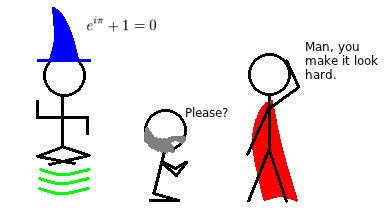
\includegraphics{Pics/SpellPoints.png}
\end{figure*}

\label{sec:MagicFocus}
Merely holding a reservoir of magical spell points in mind gives spellcasting characters a special energy. 
Spellcasting characters can put that energy to work without actually paying a spell point cost - they can become magically focused as a special use of the \nameref{sec:Concentration} skill.

If you have 1 or more spell points available, you can meditate to attempt to become magically focused. 
The DC to become magically focused is 20. Meditating is a full-round action that provokes attacks of opportunity. 
When you are magically focused, you can expend your focus on any single Concentration check you make thereafter. 
When you expend your focus in this manner, your Concentration check is treated as if you rolled a 15. 
It's like taking 10, except that the number you add to your Concentration modifier is 15. 
You can also expend your focus to gain the benefit of a magical feat - many magical feats are activated in this way.

Once you are magically focused, you remain focused until you expend your focus, become unconscious, or go to sleep (or enter a meditative trance, in the case of elves), or until your spell point reserve drops to 0.
\subsubsection{Using Stored Spell Points}
\label{sec:UsingStoredSpellPoints}
A variety of magical items exist to store spell points for later use, in particular a storage device called a \nameref{Item:PearlOfPower}. 
Regardless of what sort of item stores the spell points, all spellcasting characters must follow strict rules when tapping stored spell points.

\paragraph{A Single Source:} When using spell points from a storage item to cast a spell, a spellcasting character may not pay the spell's cost with spell points from more than one source. 
He must either use an item, his own spell point reserve, or some other discrete spell point source to pay the casting cost. 

\paragraph{Recharging:} Most spell point storage devices allow spellcasting characters to ``recharge`` the item with their own spell points. 
Doing this depletes the character's spell point reserve on a 1-for-1 basis as if he had casted a spell; however, those spell points remain indefinitely stored. 
The opposite is not true - spellcasting characters may not use spell points stored in a storage item to replenish their own spell point reserves.
\subsection{Adding Spells}
Spellcasting characters can learn new spells when they attain certain levels, as indicated on their individual class tables. %A Wizard can learn any spell from the Wizard list, including spells only available to members of his school of specialization. A Cleric can learn any spell from a domain he knows. 

\subsubsection{Spells Gained at a New Level:} Spellcasting characters perform a certain amount of personal research, prayer or meditation between adventures in an attempt to unlock latent magical abilities.
Each time a spellcasting character attains a new level, he or she learns additional spells according to his class description. 
These spells represent abilities unlocked from latency. The spells must be of levels the characters can cast (see the class table for each class).

\subsubsection{Independent Research:} 
A spellcaster also can research a spell independently, duplicating an existing spell or creating an entirely new one. 
If characters are allowed to develop new spells, use these guidelines to handle the situation.
Any kind of caster can create a new spell. 
The research involved requires access to a retreat conducive to uninterrupted research, prayer, or meditation. 
Research involves an expenditure of 200 XP per week and takes one week per level of the spell. 
At the end of that time, the character makes a \nameref{sec:Spellcraft} check (DC 10 + spell level). 
If that check succeeds, the character learns the new spell if her research produced a viable spell. 
If the check fails, the character must go through the research process again if she wants to keep trying.

Spells learned through independent research still count against the spellcaster's number of spells known.
\subsubsection{Cast an Unknown Spell from a Scroll:}
A spellcasting character can attempt to cast a spell from a source other than his own knowledge (usually a scroll, although other means of storing magical knowledge may exist, such as a magical stone tablet). 
See \nameref{Item:Scrolls} for information on how to do so.

%To do so, the character must first decipher the scroll, as described under \nameref{Item:Scrolls}.

% Next, the spellcasting character must choose one of the spells available on the scroll and read it.
% As part of reading the spell, make a \nameref{sec:Spellcraft} check 
% (DC 15 + the spell's level) to see if the spell will be correctly cast. 
% If the spell is not on the caster's class list, he automatically fails this check.
% This check requires one full round, which provokes attacks of opportunity.
% 
% Upon successfully making the check, the character can immediately attempt to cast that spell even if he doesn't know it 
% (assuming he has spell points left for the day). 
% He can attempt to cast the spell normally on his next turn.
% He retains the ability to cast the selected spell for only 1 round. 
% If he doesn't cast the spell, fails the Spellcraft check, or casts a different spell, 
% he loses his chance to cast that spell unless the source is read again.
\subsection{Special Abilities}
Magical creatures can create magical effects without having levels in a spellcasting class (although they can take a spellcasting class to further enhance their abilities); such creatures have the magical subtype.
Characters using \nameref{Item:Wands} and other magical items can also create magical effects.

\subsubsection{Spell-like Abilities}
The casting of spells by creatures without a spellcasting class (creatures with the magical subtype, also simply called magical creatures) is considered a spell-like ability (Sp). 

Usually, a magical creature's spell-like ability works just like the spell of that name. 
A few spell-like abilities are unique; these are explained in the text where they are described.
Spell-like abilities have no verbal or somatic components, but do they require an XP cost if the equivalent spell has an XP cost. 
The user activates them mentally.

A spell-like ability has a casting time of 1 standard action unless noted otherwise in the ability description. 
In all other ways, a spell-like ability functions just like a spell, notably including that using a spell-like ability provokes attacks of opportunity and is subject to interruption, and the save DCs of spell-like abilities are calculated as normal (if no key ability modifier for calculating the save DC is given, default to Charisma). 
However, a magical creature does not have to pay a spell-like ability's spell point cost.

Spell-like abilities are subject to spell resistance and to being dispelled by dispel magic. 
They do not function in areas where magic is suppressed or negated.

All creatures with spell-like abilities are assigned a caster level, which which indicates how difficult it is to dispel their spell-like effects and determines all level-dependent variables (such as range or duration) the abilities might have (like spellcasters, creatures with spell-like abilities may voluntarily lower their caster level). 
When a creature uses a spell-like ability, the spell is cast as if the creature had spent a number of spell points equal to its caster level.
If the spell has augments, it may choose those if its caster level is sufficient.
\subsubsection{Supernatural Abilities}
Some creatures have magical abilities that are considered supernatural (Su). 
Magical feats are also supernatural abilities. 

These abilities cannot be disrupted in combat, as spells can be, and do not provoke attacks of opportunity (except as noted in their descriptions). 

Supernatural abilities are not subject to spell resistance and cannot be negated or dispelled; however, they do not function in areas where magic is suppressed.
\subsection{Magical Maladies}
\subsubsection{Ability Burn}
This is a special form of ability damage that cannot be magically healed. 
It is caused by the use of certain magical feats and spells. It returns only through natural healing.

\subsubsection{Disease, Cascade Flu}
Spread by brain moles and other vermin; injury; DC 13; incubation one day; damage magical cascade.

A magical cascade is a loss of control over magical abilities. Using spell points becomes dangerous for a character infected by cascade flu, once the incubation period has run its course. 
Every time an afflicted character casts a spell, she must make a DC 16 Concentration check. 
On a failed check, a magical cascade is triggered. 
The spell operates normally, but during the following round, without the character's volition, two additional spells she knows are cast randomly, and their spell cost is deducted from the character's reserve. 
During the next round, three additional spells are cast, and so on, until all the magical character's spell points are drained. 
Spells with a range of personal or touch always affect the diseased character. 
For other spells that affect targets, roll d\%: On a 01-50 result, the spell affects the diseased character, and 51-00 indicates that the spell targets other creatures in the vicinity. 
Magical creatures (those that cast their spells without paying points) cascade until all the spells they know have been cast at least twice.
As with any disease, a spellcasting character who is injured or attacked by a creature carrying a disease or parasite, or who otherwise has contact with contaminated material, must make an immediate Fortitude save. 
On a success, the disease fails to gain a foothold. 
On a failure, the character takes damage (or incurs the specified effect) after the incubation period. 
Once per day afterward, the afflicted character must make a successful Fortitude save to avoid repeating the damage. 
Two successful saving throws in a row indicate she has fought off the disease.
\subsubsection{Disease, Cerebral Parasites}
Spread by contact with infected magical or spellcasting creatures; contact; DC 15; incubation 1d4 days; damage 1d8 spell points. 

Cerebral parasites are tiny organisms, undetectable to normal sight. 
An afflicted character may not even know he carries the parasites - until he discovers he has fewer spell points for the day than expected. 
Magical creatures with cerebral parasites are limited to using each of their known spells only once per day (instead of freely casting them). 
See the note about diseases under Cascade Flu, above.

\subsubsection{Negative Levels}
\label{sec:NegativeLevels}
Spellcasting characters can gain negative levels just like members of other character classes. 
A spellcasting character loses access to one spell per negative level from the highest level of spell he can cast; 
he also loses a number of spell points equal to the cost of that spell. 
If two or more spells fit these criteria, the caster decides which one becomes inaccessible. 
The lost spell becomes available again as soon the negative level is removed, providing the caster is capable of using it at that time. 
Lost spell points also return.
\subsection{Spell Descriptions}
The description of each spell is presented in a standard format. Each category of information is explained and defined below.
\subsubsection{Name}
The first line of every spell description gives the name by which the spell is generally known. 
A spell might be known by other names in some locales, and specific casters might have names of their own for their spells.

\subsubsection{School (Subschool)}
\label{sec:MagicalSchools}
Beneath the spell name is a line giving the school of magic (and the subschool, if appropriate) that the spell belongs to.
Every spell belongs to one of eight schools of magic. A school of magic is a group of related spells that work in similar ways.
\paragraph{Abjuration}
Abjurations are protective spells. They create physical or magical barriers, negate magical or physical abilities, harm trespassers, or even banish the subject of the spell to another plane of existence.
If an abjuration creates a barrier that keeps certain types of creatures at bay, that barrier cannot be used to push away those creatures. 
If you force the barrier against such a creature, you feel a discernible pressure against the barrier. 
If you continue to apply pressure, you end the spell.
\paragraph{Conjuration}
Each conjuration spell belongs to one of four subschools. 
Conjurations bring manifestations of objects, creatures, or some form of energy to you (the summoning subschool), actually transport creatures from another plane of existence to your plane (calling), transport creatures or objects over great distances (teleportation), or create objects or effects on the spot (creation). 
Creatures you conjure usually, but not always, obey your commands.
A creature or object brought into being or transported to your location by a conjuration spell cannot appear inside another creature or object, nor can it appear floating in an empty space. It must arrive in an open location on a surface capable of supporting it.
The creature or object must appear within the spell's range, but it does not have to remain within the range.

\subparagraph{Calling:}
A calling spell transports a creature from another plane to the plane you are on. 
% The spell grants the creature the one-time ability to return to its plane of origin, 
% although the spell may limit the circumstances under which this is possible. 
Unless otherwise noted, the spell does not grant the creature the ability to return to its plane of origin,a second spell has to be cast in order to send it home.
Creatures who are called actually die when they are killed.
The duration of a calling spell is instantaneous, which means that the called creature can't be dispelled.
A called creature cannot use any summoning or calling abilities it may have, or any spell or other ability with an XP cost.

\subparagraph{Creation:}
A creation spell manipulates matter to create an object or creature in the place the spellcaster designates (subject to the limits noted above). 
If the spell has a duration other than instantaneous, magic holds the creation together, and when the spell ends, the conjured creature or object vanishes without a trace. 
If the spell has an instantaneous duration, the created object or creature is merely assembled through magic. 
It lasts indefinitely and does not depend on magic for its existence.

\subparagraph{Summoning:}
A summoning spell instantly conjures a creature or object in a place you designate. 
When the spell ends or is dispelled, a summoned creature disappears, but a summoned object is not sent back unless the spell description specifically indicates this. 
A summoned creature also disappears if it is killed or if its hit points drop to 0 or lower.
When the spell that summoned a creature ends and the creature disappears, all the spells it has cast expire. 
A summoned creature cannot use any innate summoning or calling abilities it may have.
A summoned creature always refuses to use any spell or other ability with an XP cost.

\subparagraph{Teleportation:}
A teleportation spell transports one or more creatures or objects a great distance. 
The most powerful of these spells can cross planar boundaries. 
The transportation is (unless otherwise noted) one-way and not dispellable.
Teleportation is instantaneous travel through the Astral Plane. Anything that blocks astral travel also blocks teleportation.
\paragraph{Divination}
Divination spells enable you to learn secrets long forgotten, to predict the future, to find hidden things, and to foil deceptive spells.
Many divination spells have cone-shaped areas. These move with you and extend in the direction you look. 
The cone defines the area that you can sweep each round. 
If you study the same area for multiple rounds, you can often gain additional information, as noted in the descriptive text for the spell.

\subparagraph{Scrying:}

A scrying spell creates an invisible magical sensor that sends you information. 
Unless noted otherwise, the sensor has the same powers of sensory acuity that you possess. 
This level of acuity includes any spells or effects that target you, but not spells or effects that emanate from you. 
However, the sensor is treated as a separate, independent sensory organ of yours, and thus it functions normally even if you have been blinded, deafened, or otherwise suffered sensory impairment.
Any creature with an Intelligence score of 12 or higher can notice the sensor by making a DC 20 Intelligence check. 
The sensor can be dispelled as if it were an active spell.
Lead sheeting or magical protection blocks a scrying spell, and you sense that the spell is so blocked.
\paragraph{Enchantment}
Enchantment spells affect the minds of others, influencing or controlling their behavior.
All enchantments are mind-affecting spells. Two types of enchantment spells grant you influence over a subject creature.

\subparagraph{Charm:}
A charm spell changes how the subject views you, typically making it see you as a good friend.

\subparagraph{Compulsion:}
A compulsion spell forces the subject to act in some manner or changes the way her mind works. 
Some compulsion spells determine the subject's actions or the effects on the subject, some compulsion spells allow you to determine the subject's actions when you cast the spell, and others give you ongoing control over the subject.
\paragraph{Evocation}
Evocation spells manipulate energy or tap an unseen source of power to produce a desired end. 
In effect, they create something out of nothing. 
Many of these spells produce spectacular effects, and evocation spells can deal large amounts of damage.
\paragraph{Illusion}
Illusion spells deceive the senses or minds of others. 
They cause people to see things that are not there, not see things that are there, hear phantom noises, or remember things that never happened.

\subparagraph{Figment:}
A figment spell creates a false sensation. Those who perceive the figment perceive the same thing, not their own slightly different versions of the figment. (It is not a personalized mental impression.) 
Figments cannot make something seem to be something else. 
A figment that includes audible effects cannot duplicate intelligible speech unless the spell description specifically says it can. 
If intelligible speech is possible, it must be in a language you can speak. 
If you try to duplicate a language you cannot speak, the image produces gibberish. 
Likewise, you cannot make a visual copy of something unless you know what it looks like.
Because figments and glamers (see below) are unreal, they cannot produce real effects the way that other types of illusions can. 
They cannot cause damage to objects or creatures, support weight, provide nutrition, or provide protection from the elements. 
Consequently, these spells are useful for confounding or delaying foes, but useless for attacking them directly.
A figment's AC is equal to 10 + its size modifier.

\subparagraph{Glamer:}
A glamer spell changes a subject's sensory qualities, making it look, feel, taste, smell, or sound like something else, or even seem to disappear.

\subparagraph{Pattern:}
Like a figment, a pattern spell creates an image that others can see, but a pattern also affects the minds of those who see it or are caught in it. 
All patterns are mind-affecting spells.

\subparagraph{Phantasm:}
A phantasm spell creates a mental image that usually only the caster and the subject (or subjects) of the spell can perceive. 
This impression is totally in the minds of the subjects. It is a personalized mental impression. (It's all in their heads and not a fake picture or something that they actually see.) 
Third parties viewing or studying the scene don't notice the phantasm. All phantasms are mind-affecting spells.

\subparagraph{Shadow:}
A shadow spell creates something that is partially real from extradimensional energy. 
Such illusions can have real effects. Damage dealt by a shadow illusion is real.

\subparagraph{Saving Throws and Illusions (Disbelief):}
Creatures encountering an illusion usually do not receive saving throws to recognize 
it as illusory until they study it carefully or interact with it in some fashion.
A successful saving throw against an illusion reveals it to be false, 
but a figment or phantasm remains as a translucent outline.
A failed saving throw indicates that a character fails to notice something is amiss. 
A character faced with proof that an illusion isn't real needs no saving throw. 
If any viewer successfully disbelieves an illusion and communicates this fact to others, 
each such viewer gains a saving throw with a +4 bonus.

\paragraph{Necromancy}
Necromancy spells manipulate the power of death, unlife, and the life force. 
Spells involving undead creatures make up a large part of this school.

\subparagraph{Healing:}
Certain necromancy spells heal creatures or even bring them back to life.
\paragraph{Transmutation}
Transmutation spells change the properties of some creature, thing, or condition.

% \subparagraph{Polymorph:}  Pre-1.10 beta version
% Some Transmutation spells change the subject's form into that of another creature entirely.
% When under a Polymorph subschool spell, the subject loses some class and most racial features.
% Of your class features, you retain all but your ability to cast spells, use spell-like or supernatural abilities that require activation, and your ability to manifest psionic powers. 
% Your hit point total never changes as a result of a Polymorph subschool spell, even if your new form has a Constitution score different from your own.
% Of your racial features, you retain your bonus feats, bonus skill points, skill bonuses, your racial bonus feats, and racial weapon proficiencies. All other racial features are lost.
% You retain your own type and subtypes, and all your feats.
% Unless otherwise noted, your ability scores and natural armor bonus are unchanged from that of your natural form. You retain your ability to speak unless your new form has no organs capable of supporting speech.
% Magic items and articles of clothing not feasibly capable of being worn, held or carried by your new form meld into your body, continuing to provide their benefits.
% A creature can never be the subject of more than one Polymorph spell simultaneously. If multiple Polymorph spells are cast on a creature in succession, the older spells are suppressed while the newest is in effect.
% Recognizing that a creature is under a Polymorph spell (rather than being a normal, average member of the creature type the subject morphed into) is generally a DC 20 spot check, or DC
% 15 for members of the creature type that the subject morphed into.

\subparagraph{Polymorph:}
Some Transmutation spells change the subject's form into that of another creature entirely.
When under a Polymorph subschool spell, the subject loses most of its racial features.
Of its racial features, the subject retains its bonus feats, bonus skill points, skill bonuses, and racial weapon proficiencies. All other racial features are lost.
It retains its own type and subtypes.
Unless otherwise noted, its ability scores and natural armor bonus are unchanged from that of its natural form. It retains its ability to speak unless the new form has no organs capable of supporting speech (assume that animalistic mouths are sufficient for providing speech).
Magic items and articles of clothing not feasibly capable of being worn, held or carried by the new form meld into the subject's body, continuing to provide their benefits if applicable.
A creature can never be the subject of more than one Polymorph spell simultaneously. If multiple Polymorph spells are cast on a creature in succession, the older spells are suppressed while the newest is in effect.
Recognizing that a creature is under a Polymorph spell (rather than being a normal, average member of the creature type the subject morphed into) is generally a DC 20 spot check, or DC
15 for members of the creature type that the subject morphed into.
Your hit point total never changes as a result of a Polymorph subschool spell, even if your new form has a Constitution score different from your own.
\subsubsection{Descriptor}
Appearing on the same line as the school and subschool (when applicable) is a descriptor that further categorizes the spell in some way. 
Some spells have more than one descriptor, some have none. Descriptors are shown in brackets.

The descriptors that apply to spells are 
\emph{acid, air, chaotic, cold, darkness, death, earth, electricity, evil, fear, fire, force, good, language-dependent, lawful, light, mind-affecting, minion, sonic,} and \emph{water.} 

Most of these descriptors have no game effect by themselves, but they govern how the spell interacts with other spells, with special abilities, with unusual creatures, with alignment, and so on.

\paragraph{Language-dependent spells} use intelligible language as a medium.

\paragraph{Mind-affecting spells} work only against creatures with an Intelligence score of 1 or higher.

\paragraph[Minion]{Minion Spells} 
\label{sec:MinionSpells}
are spells that place minions of one kind or another under your control for an extended period of 
time (often permanently).
Regardless of the number of different spells that give you minions, you can control only (2 + your charisma modifier) HD worth of creatures per character level (minimum 1 HD worth of creatures per level, if your charisma is 8 or lower). 
If you exceed this number, you must immediately release enough creatures from your control to bring you beneath the limit again.
In the case of active spells that give you ongoing control, the spells immediately expire.
In the case of creatures you have created being under your control, the creatures immediately become uncontrolled.
\subsubsection{Level}
The next line of the spell description gives a spell's level, a number between 1 and 9 that defines the spell's relative strength. 
This number is preceded by the name of the class whose members can cast the spell.
\subsubsection{Components}
\label{sec:Components}
When a spell is cast, a component may be needed to facilitate the spell. This component may be somatic or verbal.

\paragraph{Verbal components (V)} A verbal component is a spoken incantation. 
To provide a verbal component, you must be able to speak in a strong voice. 
A \nameref{Spell:Silence} spell or a gag spoils the incantation (and thus the spell). 
A spellcaster who has been deafened has a 20\% chance to spoil any spell he tries to cast with a verbal component.

\paragraph{Somatic components (S)} A somatic component is a measured and precise movement of the hand. 
You must have at least one hand free to provide a somatic component.

\paragraph{Dispense with Components:} Despite the fact that almost every spell has a component, a spellcasting character can always choose to attempt to cast the spell without the flashy accompaniment of magical words and hand gestures, usually to avoid attention or to circumvent a condition that prevents him from using components (see above). 
To cast a spell without any components (no matter how many components it might have), a caster must make a Concentration check (DC 15 + the level of the spell).
This check is part of the action of casting the spell. If the check is unsuccessful, the components are needed if the spell is to go off.
Even if a caster casts a spell without a component, he is still subject to attacks of opportunity in appropriate circumstances. 
(Of course, another Concentration check can be made as normal to either cast defensively or maintain the spell if attacked.)

\subsubsection{Casting Time}
Most spells have a casting time of 1 standard action. Others take 1 round or more, while a few require only a free action.
A spell that takes 1 round to cast requires a full-round action. 
It comes into effect just before the beginning of your turn in the round after you began casting the spell. 
You then act normally after the spell is completed. 
A spell that takes 1 minute to cast comes into effect just before your turn 1 minute later (and for each of those 10 rounds, you are casting a spell as a full-round action, as noted above for 1-round casting times). 
These actions must be consecutive and uninterrupted, or the spell points are lost and the spell fails.
When you use a spell that takes 1 round or longer to cast, you must continue the concentration from the current round to just before your turn in the next round (at least). 
If you lose concentration before the casting time is complete, the spell points are lost and the spell fails.
You make all pertinent decisions about a spell (range, target, area, effect, version, and so forth) when the spell comes into effect.

\subsubsection{Range}
A spell's range indicates how far from you it can reach, as defined in the Range entry of the spell description. 
A spell's range is the maximum distance from you that the spell's effect can occur, as well as the maximum distance at which you can designate the spell's point of origin. 
If any portion of the area would extend beyond the range, that area is wasted. Standard ranges include the following:

\paragraph{Personal:} The spell affects only you.

\paragraph{Touch:} You must touch a creature or object to affect it. A touch spell that deals damage can score a critical hit just as a weapon can. 
A touch spell threatens a critical hit on a natural roll of 20 and deals double damage on a successful critical hit. 
Some touch spells allow you to touch multiple targets. 
You can touch as many willing targets as you can reach, but all targets of the spell must be touched in the same round that you cast the spell.

\paragraph{Close:} The spell reaches as far as 25 feet away from you. The maximum range increases 5 feet for every two caster levels you have.

\paragraph{Medium:} The spell reaches as far as 100 feet + 10 feet per caster level.

\paragraph{Long:} The spell reaches as far as 400 feet + 40 feet per caster level.

\paragraph{Range Expressed in Feet:} Some spells have no standard range category, just a range expressed in feet.

\subsubsection{Aiming a Spell}
You must make some choice about whom the spell is to affect or where the spell's effect is to originate, 
depending on the type of spell. The next entry in a spell description defines the spell's target (or targets), its effect, or its area, as appropriate.

\paragraph{Target or Targets:} Some spells have a target or targets. You cast these spells on creatures or objects, as defined by the spell itself. 
You must be able to see or touch the target, and you must specifically choose that target. 
However, you do not have to select your target until you finish casting the spell.
If you cast a targeted spell on the wrong type of target the spell has no effect. 
If the target of a spell is yourself (the spell description has a line that reads ''Target: You``), 
you do not receive a saving throw and spell resistance does not apply. 
The Saving Throw and Spell Resistance lines are omitted from such spells.
Some spells can be cast only on willing targets. 
Declaring yourself as a willing target is something that can be done at any time (even if you're flat-footed or it isn't your turn). 
Unconscious creatures are automatically considered willing, but a character who is conscious but immobile or helpless (such as one who is bound, cowering, grappling, paralyzed, pinned, or stunned) is not automatically willing. 
The Saving Throw and spell Resistance lines are usually omitted from such spells, since only willing subjects can be targeted.

\paragraph{Effect:} Some spells, such as most conjuration spells, create things rather than affect things that are already present. 
Unless otherwise noted in the spell description, you must designate the location where these things are to appear, either by seeing it or defining it. Range determines how far away an effect can appear, but if the effect is mobile, it can move regardless of the spell's range once created.

\paragraph{Ray:} Some effects are rays. You aim a ray as if using a ranged weapon, though typically you make a ranged touch attack rather than a normal ranged attack. 
As with a ranged weapon, you can fire into the dark or at an invisible creature and hope you hit something. 
You don't have to see the creature you're trying to hit, as you do with a targeted spell. 
Intervening creatures and obstacles, however, can block your line of sight or provide cover for the creature you're aiming at.
If a ray spell has a duration, it's the duration of the effect that the ray causes, not the length of time the ray itself persists.
If a ray spell deals damage, you can score a critical hit just as if it were a weapon. 
A ray spell threatens a critical hit on a natural roll of 20 and deals double damage on a successful critical hit.

\paragraph{Spread:} Some effects spread out from a point of origin (which may be a grid intersection, or may be the caster) to a distance described in the spell. The effect can extend around corners and into areas that you can't see. 
Figure distance by actual distance traveled, taking into account turns the effect may take. 
When determining distance for spread effects, count around walls, not through them. 
As with movement, do not trace diagonals across corners. 
You must designate the point of origin for such an effect (unless the effect is centered on you), but you need not have line of effect (see below) to all portions of the effect.

\paragraph{(S) Shapeable:} If an Effect line ends with ''(S)`` you can shape the spell. 
A shaped effect can have no dimension smaller than 10 feet.

\paragraph{Area:} Some spells affect an area. Sometimes a spell description specifies a specially defined area, but usually an area falls into one of the categories defined below.
Regardless of the shape of the area, you select the point where the spell originates, but otherwise you usually don't control which creatures or objects the spell affects. 
The point of origin of a spell that affects an area is always a grid intersection. 
When determining whether a given creature is within the area of a spell, count out the distance from the point of origin in squares just as you do when moving a character or when determining the range for a ranged attack. 
The only difference is that instead of counting from the center of one square to the center of the next, you count from intersection to intersection.
You can count diagonally across a square, but every second diagonal counts as 2 squares of distance. 
If the far edge of a square is within the spell's area, anything within that square is within the spell's area. 
If the spell's area touches only the near edge of a square, however, anything within that square is unaffected by the spell.

\subparagraph{Burst, Emanation, or Spread:} Most spells that affect an area function as a burst, an emanation, or a spread. 
In each case, you select the spell's point of origin and measure its effect from that point. 

A burst spell affects whatever it catches in its area, even including creatures that you can't see. 
It can't affect creatures with total cover from its point of origin (in other words, its effects don't extend around corners). 
The default shape for a burst effect is a sphere, but some burst spells are specifically described as cone-shaped.

A burst's area defines how far from the point of origin the spell's effect extends.

An emanation spell functions like a burst spell, except that the effect continues to radiate from the point of origin for the duration of the spell.

A spread spell spreads out like a burst but can turn corners. You select the point of origin, and the spell spreads out a given distance in all directions. 
Figure the area the spell effect fills by taking into account any turns the effect takes.

\subparagraph{Cone, Line, or Sphere:} Most spells that affect an area have a particular shape, such as a cone, line, or sphere. 

A cone-shaped spell shoots away from you in a quarter-circle in the direction you designate. 
It starts from any corner of your square and widens out as it goes. 
Most cones are either bursts or emanations (see above), and thus won't go around corners.

A line-shaped spell shoots away from you in a line in the direction you designate. 
It starts from any corner of your square and extends to the limit of its range or until it strikes a barrier that blocks line of effect. 
A line-shaped spell affects all creatures in squares that the line passes through or touches.

A sphere-shaped spell expands from its point of origin to fill a spherical area. Spheres may be bursts, emanations, or spreads.

\subparagraph{Other:} A spell can have a unique area, as defined in its description.

\paragraph{Line of Effect:} A line of effect is a straight, unblocked path that indicates what a spell can affect. 
A solid barrier cancels a line of effect, but it is not blocked by fog, darkness, and other factors that limit normal sight. 
You must have a clear line of effect to any target that you cast a spell on or to any space in which you wish to create an effect. 
You must have a clear line of effect to the point of origin of any spell you cast.
A burst, cone, or emanation spell affects only an area, creatures, or objects to which it has line of effect from its origin (a spherical burst's center point, a cone-shaped burst's starting point, or an emanation's point of origin). 
An otherwise solid barrier with a hole of at least 1 square foot through it does not block a spell's line of effect. 
Such an opening means that the 5-foot length of wall containing the hole is no longer considered a barrier for the purpose of determining a spell's line of effect.

\subsubsection{Duration}
A spell's Duration line tells you how long the magical energy of the spell lasts.

\paragraph{Timed Durations:} Many durations are measured in rounds, minutes, hours, or some other increment. When the time is up, the magical energy sustaining the effect fades, and the spell ends. If a spell's duration is variable it is rolled secretly.

\paragraph{Instantaneous:} The magical energy comes and goes the instant the spell is cast, though the consequences might be long-lasting or permanent.

\paragraph{Permanent:} The energy remains as long as the effect does. This means the spell is vulnerable to dispel magic.

\paragraph{Concentration:} The spell lasts as long as you concentrate on it. Concentrating to maintain a spell is a standard action that does not provoke attacks of opportunity. Anything that could break your concentration when casting a spell can also break your concentration while you're maintaining one, causing the spell to end. You can't cast a spell while concentrating on another one. Some spells may last for a short time after you cease concentrating. In such a case, the spell keeps going for the given length of time after you stop concentrating, but no longer. Otherwise, you must concentrate to maintain the spell, but you can't maintain it for more than a stated duration in any event. If a target moves out of range, the spell reacts as if your concentration had been broken.

\paragraph{Subjects, Effects, and Areas:} If the spell affects creatures directly the result travels with the subjects for the spell's duration. If the spell creates an effect, the effect lasts for the duration. The effect might move or remain still. Such an effect can be destroyed prior to when its duration ends. If the spell affects an area then the spell stays with that area for its duration. Creatures become subject to the spell when they enter the area and are no longer subject to it when they leave.

\paragraph{Touch Spells and Holding the Charge:} In most cases, if you don't discharge a touch spell on the round you cast it, you can hold the charge (postpone the discharge of the spell) indefinitely. You can make touch attacks round after round. If you touch anything with your hand while holding a charge, the spell discharges. If you cast another spell, the touch spell dissipates.
Some touch spells allow you to touch multiple targets as part of the spell. You can't hold the charge of such a spell; you must touch all the targets of the spell in the same round that you finish casting the spell. You can touch one friend (or yourself) as a standard action or as many as six friends as a full round action.

\paragraph{Discharge:} Occasionally a spell lasts for a set duration or until triggered or discharged.

\paragraph{(D) Dismissible:} If the Duration line ends with ''(D),`` you can dismiss the spell at will. You must be within range of the spell's effect and must mentally will the dismissal, which uses the same components as when you first cast the spell. Dismissing a spell is a standard action that does not provoke attacks of opportunity. A spell that depends on concentration is dismissible by its very nature, and dismissing it does not take an action or require a component, since all you have to do to end the spell is to stop concentrating on your turn.

\subsubsection{Saving Throw}
\label{sec:SavingThrow}
Usually a harmful spell allows a target to make a saving throw to avoid some or all of the effect. 
The Saving Throw line in a spell description defines which type of saving throw the spell allows and describes how saving throws against the spell work.

\paragraph{Negates:} The spell has no effect on a subject that makes a successful saving throw.

\paragraph{Partial:} The spell causes an effect on its subject, such as death. A successful saving throw means that some lesser effect occurs (such as being dealt damage rather than being killed).

\paragraph{Half:} The spell deals damage, and a successful saving throw halves the damage taken (round down). 

\paragraph{None:} No saving throw is allowed.

\paragraph{(object):} The spell can be cast on objects, which receive saving throws only if they are magical or if they are attended (held, worn, grasped, or the like) by a creature resisting the spell, in which case the object uses the creature's saving throw bonus unless its own bonus is greater. (This notation does not mean that a spell can be cast only on objects. Some spells of this sort can be cast on creatures or objects.) A magic item's saving throw bonuses are each equal to 2 + one-half the item's caster level.

\paragraph{(harmless):} The spell is usually beneficial, not harmful, but a targeted creature can attempt a saving throw if it desires.

\paragraph{Saving Throw Difficulty Class:} 

A saving throw against your spell has a DC of
\begin{quote}
\centering
\large 
 {10 + one-half the number of spell points spent on the spell (round up) + your key ability modifier.}
%\normalsize
\end{quote}
Count all spell points spent on augmenting a spell in order to determine its spell point cost for this purpose, 
but do not count the additional spell point cost incurred by adding a metamagic feat to a spell.\footnote{This is a new, and most fundamental rule.}

\paragraph{Succeeding on a Saving Throw:} A creature that successfully saves against a spell that has no obvious physical effects feels a hostile force or a tingle, but cannot deduce the exact nature of the attack unless it succeeds on the appropriate \nameref{sec:Spellcraft} check. 
Likewise, if a creature's saving throw succeeds against a targeted spell you sense that the spell has failed. 
You do not sense when creatures succeed on saves against effect and area spells.

\paragraph{Failing a Saving Throw against Mind-Affecting Spells:} If you fail your save, you are unaware that you have been affected by a spell.

\paragraph{Automatic Failures and Successes:} A natural 1 (the d20 comes up 1) on a saving throw is always a failure, and the spell may deal damage to exposed items (see Items Surviving after a Saving Throw, below). A natural 20 (the d20 comes up 20) is always a success.

\paragraph{Voluntarily Giving up a Saving Throw:} A creature can voluntarily forego a saving throw and willingly accept a spell's result. Even a character with a special resistance to magic can suppress this quality.
A creature  can under no conditions whatsoever be directly forced to give up its saving throw, even with Enchantment spells or the control granted over a Called creature.

\paragraph{Items Surviving after a Saving Throw:} Unless the descriptive text for the spell specifies otherwise, all items carried or worn by a creature are assumed to survive a magical attack.

\subsubsection{Spell Resistance}
Spell resistance is a special defensive ability. If your spell is being resisted by a creature with spell resistance, you must make a caster level check (d20 + caster level) at least equal to the creature's spell resistance for the spell to affect that creature. The defender's spell resistance functions like an Armor Class against magical attacks.\footnote{Power resistance is equivalent to spell resistance unless the Psionics Is Different option is in use.} Include any adjustments to your caster level on this caster level check.
The Spell Resistance line and the descriptive text of a spell description tell you whether spell resistance protects creatures from the spell. In many cases, spell resistance applies only when a resistant creature is targeted by the spell, not when a resistant creature encounters a spell that is already in place.
The terms “object” and “harmless” mean the same thing for spell resistance as they do for saving throws. A creature with spell resistance must voluntarily lower the resistance (a standard action) to be affected by a spell noted as harm less. In such a case, you do not need to make the caster level check described above.

\subsubsection{Spell Points}
All spells have a Spell Points line, indicating the spell's cost. This is the minimum number of spell points that must be paid in order to cast the spell.
The spellcasting character class tables show how many spell points a character has access to each day, depending on level.
A spell's cost is determined by its spell level, as shown on the Spell Points by Spell Level table. %table \ref{tab:SpellPointsBySpellLevel}. 
Every spell's cost is noted in its description for ease of reference.
\begin{center}
\resizebox{7cm}{!}{
\begin{tabular}{|l|*{9}{c|}}
\multicolumn{10}{c}{\textbf{Spell Points by Spell Level}}\\
\hline
\textbf{Level}&1&2&3&4&5&6&7&8&9\\
\hline
\textbf{Cost}&1&3&5&7&9&11&13&15&17\\
\hline
\end{tabular}}
\end{center}

\paragraph{Spell Point Limit:} 
The spell point cost mentioned in each spell's description is the minimum number of spell points needed to cast the spell. 
You can, if you wish, spend more than this minimum number on a spell, usually to increase the spell's saving throwDC, or to use an augment the spell may have.
The maximum number of points you can spend on a spell (for any reason) is equal to your caster level (the fundamental rule of magic).

\paragraph{XP Cost (XP):} On the same line that the spell point cost of a spell is indicated, the spell's experience point cost, if any, is noted. Particularly powerful effects entail an experience point cost to you. No spell or power can restore XP lost in this manner. You cannot spend so much XP that you lose a level, so you cannot cast a spell with an XP cost unless you have enough XP to spare. However, you can, on gaining enough XP to attain a new level, use those XP for casting a spell rather than keeping them and advancing a level. The XP are expended when you cast the spell, whether or not the casting succeeds.

\subsubsection{Flavor Text}
Most spells have a sentence or two of ''flavor text`` - text that has no immutable meaning, but provides an example of how characters might understand or perceive the spell, or an explanation of how the spell might fit into a campaign.
If this flavor text does not fit the way you imagine the spell, this flavor text should be discarded and replaced with a description of your own making.

\subsubsection{Descriptive Text}
This portion of a spell description details what the spell does and how it works. If one of the previous lines in the description included ''see text,`` this is where the explanation is found. If the spell you're reading about is based on another spell you might have to refer to a different spell for the “see text” information. If a spell is the equivalent of a spell an entry of “see spell text” directs you to the appropriate spell description.

\paragraph[Augment]{Augment:} 
\label{sec:Augment}
Many spells have variable effects based on the number of spell points you spend when you cast them. The more points spent, the more powerful the spell. How this extra expenditure affects a spell is specific to the spell. Some augmentations allow you to increase the number of damage dice, while others extend a spell's duration or modify a spell in unique ways. Each spell that can be augmented includes an entry giving how many spell points it costs to augment and the effects of doing so. However, you can spend only a total number of points on a spell equal to your caster level.
Augmenting a spell takes place as part of another action (casting a spell). Unless otherwise noted in the Augment section of an individual spell description, you can augment a spell only at the time you cast it. Some Augments radically alter the spell's characteristics.
\subsection{Epic Magic}
Epic magic is very cool and will definitely be implemented one day. \newpage

\part{Races and Classes}
As the base system is changed, races and classes must be adapted as well. The following three chapters deal with updating player races that deal with magic, the base classes, as well as the prestige classes presented in the \href{http://www.wizards.com/default.asp?x=d20/article/srd35}{d20 srd} to consistently work with the updated underlying system.
\section{Races}
Many creatures have innate magical powers on the racial level, every member of the species possessing some measure of magical talent. None of the common races have powers as pronounced as those of strong magical beings like dragons and rakshasas, but some, like gnomes and some elves, still have sufficient abilities to affect their daily lives and preferred fighting styles.

Unless noted otherwise in this chapter, use the rules text presented in the \href{http://www.wizards.com/default.asp?x=d20/article/srd35}{d20 srd}.\footnote{To summarize the changes to races: Elves gain 2 bonus spell points. Gnomes have their spell-like abilities updated to reflect the changes in the spells they refer to.}
\subsection{Elves}
\subsubsection{Description}
Elves average 5 feet tall and typically weigh just over 100 pounds. They live on fruits and grains, though they occasionally hunt for fresh meat. Elves prefer colorful clothes, usually with a green-and-gray cloak that blends well with the colors of the forest.

Elves speak Elven, and most also know Common and Sylvan.
\subsubsection{Magic}
Elves have a natural talent for magic, the race having spawned many of the world's most famous (and oldest) archmages. The race is especially well known for its numerous Wizards.
\subsubsection{Combat}
Elves are cautious warriors and take time to analyze their opponents and the location of the fight if at all possible, maximizing their advantage by using ambushes, snipers, and camouflage. They prefer to fire from cover and retreat before they are found, repeating this maneuver until all of their enemies are dead.

They prefer longbows, shortbows, rapiers, and longswords. In melee, elves are graceful and deadly, using complex maneuvers that are beautiful to observe. Their wizards often use \nameref{Spell:Sleep} spells during combat because these won't affect other elves.
\subsubsection{Racial Traits}
Elves possess the following racial traits.

\begin{list}{\labelitemi}{\leftmargin=1em}
 \item +2 Dexterity, -2 Constitution.
 \item Medium size.
 \item An elf's base land speed is 30 feet.
 \item Immunity to sleep spells and effects, and a +2 racial saving throw bonus against enchantment spells or effects.
 \item Low-light vision.
 \item Weapon Proficiency: Elves are automatically proficient with the longsword, rapier, longbow, composite longbow, shortbow, and composite shortbow.
 \item +2 racial bonus on Listen, Search, and Spot checks. An elf who merely passes within 5 feet of a secret or concealed door is entitled to a Search check to notice it as if she were actively looking for it.
 \item Naturally magical: Elves gain 2 bonus spell points at 1st level. This does not grant them the ability to cast spells unless they gain that ability through another source, such as levels in a spellcasting class.
 \item Automatic Languages: Common, Elven. Bonus Languages: Draconic, Gnoll, Gnome, Goblin, Orc, Sylvan.
 \item Favored Class: \nameref{sec:Wizard}.
\end{list}
\subsection{Gnomes}
\subsubsection{Description}
Gnomes stand 3 to 3½ feet tall and weigh 40 to 45 pounds. Their skin color ranges from dark tan to woody brown, their hair is fair, and their eyes can be any shade of blue. Gnome males prefer short, carefully trimmed beards. Gnomes generally wear leather or earth tones, though they decorate their clothes with intricate stitching or fine jewelry. Gnomes reach adulthood at about age 40, and they live about 350 years, though some can live almost 500 years.

Gnomes speak their own language, Gnome. Most gnomes who travel outside gnome lands (as traders, tinkers, or adventurers) know Common, while warriors in gnome settlements usually learn Goblin.
\subsubsection{Magic}
Gnomes have specific affinity with illusion magic, and the ability to communicate with burrowing animals. Some are able to use Cantrips.

Most gnome spellcasters are Bards. Those with a more scholarly bent usually become Illusionists.
\subsubsection{Combat}
Gnomes prefer misdirection and deception over direct confrontation.

They would rather befuddle or embarrass foes (other than goblinoids or kobolds) than kill them.

Gnomes make heavy use of illusion magic and carefully prepared ambushes and traps whenever they can.
\subsubsection{Racial Traits}
Gnomes have the following racial traits: 

\begin{list}{\labelitemi}{\leftmargin=1em}
 \item +2 Constitution, -2 Strength.
 \item Small: As a Small creature, a gnome gains a +1 size bonus to Armor Class, a +1 size bonus on attack rolls, and a +4 size bonus on Hide checks, but he uses smaller weapons than humans use, and his lifting and carrying limits are three-quarters of those of a Medium character.
 \item Gnome base land speed is 20 feet.
 \item Low-Light Vision: A gnome can see twice as far as a human in starlight, moonlight, torchlight, and similar conditions of poor illumination. He retains the ability to distinguish color and detail under these conditions.
 \item Weapon Familiarity: Gnomes may treat gnome hooked hammers as martial weapons rather than exotic weapons.
 \item +2 racial bonus on saving throws against illusions.
 \item Add +1 to the Difficulty Class for all saving throws against illusion spells cast by gnomes. This adjustment stacks with those from similar effects.
 \item +1 racial bonus on attack rolls against kobolds and goblinoids.
 \item +4 dodge bonus to Armor Class against monsters of the giant type. Any time a creature loses its Dexterity bonus (if any) to Armor Class, such as when it's caught flat-footed, it loses its dodge bonus, too.
 \item +2 racial bonus on Listen checks.
 \item +2 racial bonus on Craft (alchemy) checks.
 \item Automatic Languages: Common and Gnome. Bonus Languages: Draconic, Dwarven, Elven, Giant, Goblin, and Orc. In addition, a gnome can speak with a burrowing mammal (see below).
 \item Spell-Like Abilities: 1/day-\nameref{Spell:ConverseWithNature}. Caster level 1st (regardless of character level). This spell-like ability only allows the gnome to communicate with burrowing mammals, not any kind of animal. This spell-like ability qualifies gnomes as magical creatures, but still does not allow them to obtain a magical focus unless they obtain an actual spell point reserve.
 \item Cantrips: A gnome who obtains a spell point reserve (gnomes frequently have the \nameref{Feat:MagicalSpark} feat for \nameref{Spell:Ventriloquism}) can use \nameref{sec:Cantrips} as a Wizard can, albeit in a limited fashion. A gnome cannot use his racial Cantrip to deal damage, to decipher inscriptions, or to increase his reading speed. A gnome who gains Cantrips as a class feature can access all of its functions, as normal.
 \item Favored Class: \nameref{sec:Bard}.
\end{list}
 \newpage
\section{Spellcasting Classes}
\subsection[Bard]{The Bard}
\label{sec:Bard}
\begin{quote}
\emph{``I don't mean to brag, but when I sing, the angels themselves come down from their heavens to admire the brilliance.''}
- Cassius, human Bard
\end{quote}
A Bard is an arcane spellcaster whose magic manifests in the form of music or other creative or inspiring ways.

\begin{table*}
\centering
\caption{The Bard}
\label{tab:Bard}
\makebox[\textwidth]{
\begin{tabular}{llccclccc}
\toprule
	&	&	&	&	&		&\multicolumn{3}{c}{Spellcasting}\\ \cmidrule(r){7-9}
Level	&BAB	&Fort 	&Ref 	&Will 	&Special	&SP/day	&Known&Max level\\
\midrule
1st	&+0		&+0	&+2	&+2	&Bardic Performance, Bardic		&0	&2	&1st\\
	&		&	&	&	&Knowledge, Cantrips			&	&	&\\
2nd	&+1		&+0	&+3	&+3	&-					&2	&3	&1st\\
3rd	&+2		&+1	&+3	&+3	&Bardic Performance			&4	&4	&1st\\
4th	&+3		&+1	&+4	&+4	&-					&8	&5	&2nd\\
5th	&+3		&+1	&+4	&+4	&-					&12	&6	&2nd\\
6th	&+4		&+2	&+5	&+5	&Bardic Performance			&18	&7	&2nd\\
7th	&+5		&+2	&+5	&+5	&-					&24	&8	&3rd\\
8th	&+6/+1		&+2	&+6	&+6	&-					&32	&9	&3rd\\
9th	&+6/+1		&+3	&+6	&+6	&-					&40	&10	&3rd\\
10th	&+7/+2		&+3	&+7	&+7	&Bardic Performance			&50	&11	&4th\\
11th	&+8/+3		&+3	&+7	&+7	&-					&60	&12	&4th\\
12th	&+9/+4		&+4	&+8	&+8	&-					&72	&13	&4th\\
13th	&+9/+4		&+4	&+8	&+8	&-					&84	&14	&5th\\
14th	&+10/+5		&+4	&+9	&+9	&Bardic Performance			&98	&15	&5th\\
15th	&+11/+6/+1	&+5	&+9	&+9	&-					&112	&16	&5th\\
16th	&+12/+7/+2	&+5	&+10	&+10	&-					&128	&17	&6th\\
17th	&+12/+7/+2	&+5	&+10	&+10	&-					&144	&18	&6th\\
18th	&+13/+8/+3	&+6	&+11	&+11	&Bardic Performance			&162	&19	&6th\\
19th	&+14/+9/+4	&+6	&+11	&+11	&-					&180	&20	&6th\\
20th	&+15/+10/+5	&+6	&+12	&+12	&Bardic Performance			&200	&21	&6th\\
\bottomrule
\end{tabular}}
\end{table*}

\paragraph{Alignment:} Any nonlawful
\paragraph{Hit Die:} d6
\paragraph{Class skills:}
The Bard's class skills (and the key ability for each skill) are 
class skills (and the key ability for each skill) are Appraise (Int), Balance (Dex), Bluff (Cha), Climb (Str), Concentration (Con), Craft (Int), Decipher Script (Int), Diplomacy (Cha), Disguise (Cha), Escape Artist (Dex), Gather Information (Cha), Hide (Dex), Jump (Str), Knowledge (all skills, taken individually) (Int), Listen (Wis), Move Silently (Dex), Perform (Cha), Profession (Wis), Sense Motive (Wis), Sleight of Hand (Dex), Speak Language (N/A), Spellcraft (Int), Swim (Str), Tumble (Dex), and Use Magic Device (Cha).
\paragraph{Skill Points at 1st Level:} (6 + Int modifier) $\times$ 4.
\paragraph{Skill Points at each additional Level:} 6 + Int modifier.

\subsubsection{Class Features}
All the following are class features of the Bard.

\paragraph{Weapon and Armor Proficiency:} 
A Bard is proficient with all simple weapons, plus the longsword, rapier, sap, short sword, shortbow, and whip. 
Bards are proficient with light armor and shields (except tower shields).
Armor does not interfere with the casting of spells.

\paragraph{Spell Points/Day:} 
A Bard's ability to cast spells is limited by the spell points he has available. 
His base daily allotment of spell points is given on \nameref{tab:Bard} table. 
In addition, he receives bonus spell points per day if he has a high Charisma score.
His race may also provide bonus spell points per day, as may certain feats and items.

\paragraph{Spells Known:} A Bard begins play knowing two Bard spells of your choice. 
Each time he achieves a new level, he unlocks the knowledge of new spells.
Choose the spells known from the full Bard spell list.
(Exception: The feats Expanded Knowledge and Epic Expanded Knowledge 
do allow a Bard to learn spells of other classes, 
including spells restricted to specialist Wizards.) 

A Bard can cast any spell he knows that has a spell point cost equal to or lower than his caster level.
The number of times a Bard can cast spells in a day is limited only by his daily spell points. 
A Bard simply knows his spells; they are ingrained in his mind, 
though he must get a good night's sleep each day to regain all his spent spell points.
The Difficulty Class for saving throws against Bard spells is 10 + one-half the number of spell points spent on the spell (round up) + the Bard's Charisma modifier. 

Spells learned via the Bard class are arcane spells.
\paragraph{Maximum Spell Level Known:} A Bard begins play with the ability to learn 1st-level spells. 
As he attains higher levels, a Bard may gain the ability to master more complex spells, as shown on \nameref{tab:Bard} table.
To learn or cast a spell, a Bard must have a Charisma score of at least 10 + the spell's level.

\paragraph[Cantrips]{Cantrips (Su):} 
A Bard can use \nameref{sec:Cantrips} as a \nameref{sec:Wizard} can.

\paragraph{Bardic Performance:}
A Bard is trained to use the Perform skill to create magical effects on himself and those around him. At first level, he knows one type of Bardic Performance. At Bard levels 3, 5, 10, 14, 18, and 20, he learns an additional type of Bardic Performance if he has enough ranks in a Perform skill to do so. If he does not have enough ranks in a Perform skill to qualify for a new type of Bardic Performance when he is entitled to one, he does not gain one, but can (and must) select one immediately if he ever gains the required number of ranks in a Perform skill.

% He can use this ability for a number of rounds per day equal to 4 + his Charisma modifier. At each level after 1st a Bard can use Bardic Performance for 2 additional rounds per day. Each round, The Bard can produce any one of the types of Bardic Performance that he has mastered, as indicated by his level.

Starting a Bardic Performance is a standard action and requires the expenditure of the Bard's magical focus, but it can be maintained each round as a free action. 
Changing a Bardic Performance from one effect to another requires the Bard to stop the previous Performance and start a new one. 
A Bardic Performance ends immediately if the Bard is killed, paralyzed, stunned, knocked unconscious, or otherwise prevented from taking a free action to perform it each round. 
A Bard's Bardic Performance does not expire, nor does it need to be dismissed, it lasts until the Bard stops maintaining the Performance, and for five rounds thereafter. 
A Bard cannot have maintain more than one Bardic Performance in a round (but previous performances still remain in effect until they expire if a Bard ceases to maintain one Bardic Performance in favor of another). 
A Bard cannot cast spells in any round in which he maintains a Bardic Performance, but his actions are not otherwise restricted (unless the use of his Perform skill physically requires it).

Each Bardic Performance has audible components, visual components, or both, as appropriate to the Perform skill being applied.

If a Bardic Performance has audible components, the targets must be able to hear the Bard for the Performance to have any effect, and such Performances are language dependent. A deaf Bard has a 20\% change to fail when attempting to use a Bardic Performance with an audible component. If he fails this check, the action is wasted, and the Bard's magical focus is still expended. Deaf creatures are immune to Bardic Performances with audible components.

If a Bardic Performance has a visual component, the targets must have line of sight to the Bard for the Performance to have any effect. A blind Bard has a 50\% chance to fail when attempting to use a Bardic Performance with a visual component. If he fails this check, the action is wasted, and the Bard's magical focus is still expended. Blind creatures are immune to Bardic Performances with visual components.

The types of Bardic Performance are as follows:
\subparagraph{Counterperformance (Su):}
The Bard can counter magic effects that depend on sound (but not spells that were merely cast with verbal components). 
This can take one of two forms:
 
\begin{itemize}
 \item \emph{Augment saves:} The Bard makes a Perform skill check each round he maintains this form of Counterperformance.
Any creature that can perceive the Bard's Performance that is affected by a sonic or language-dependent magical attack may use the Bard's Perform check result in place of its saving throw if, after the saving throw is rolled, the Perform check result proves to be higher. 
If a creature that perceives a counterperformance is already under the effect of a non-instantaneous sonic or language-dependent magical attack, it gains another saving throw against the effect each round it hears the counterperformance, but it must use the Bard's Perform skill check result for the save. 
This form of Counterperformance does nothing against effects that don't allow saves.
 \item \emph{Performance duel:} To use this ability, the Bard makes a Perform check, opposed by the Perform check of another Bard who is starting or maintaining a Bardic Performance. Both Bards must be able to perceive each others' performances. On a successful check, the Bard using Counterperformance immediately causes the Bardic Performance started or being maintained by the other Bard to end as if the other Bard had failed to maintain the Bardic Performance and the effect then expired.
 Alternatively, this use of Counterperformance can cause one Bardic Performance started and then abandoned (no longer maintained) by another Bard to immediately expire, with no opposed check required. The Bard must have perceived the Performance before it was abandoned for this use to be possible.
 Unlike most uses of Bardic Performance, this kind of Counterperformance is instantaneous in nature
\end{itemize}

A Bard must have 4 ranks in a Perform skill to learn or use Counterperformance.
\subparagraph{Fascinate (Su):}
The Bard can use Bardic Performance to cause one or more creatures to become fascinated with him. % Each creature to be fascinated must be perceive the Performance, and able to pay attention. The Bard must also be able to perceive the creature. 
The distraction of a nearby combat or other dangers prevents the ability from working. There is no limit to the number of creatures a Bard can fascinate at a time.

To use the ability, the Bard makes a Perform check. His check result is the DC for each affected creature's Will save against the effect. If a creature's saving throw succeeds, the Bard cannot attempt to fascinate that creature again for 24 hours. If its saving throw fails, the creature sits quietly and enjoys the Performance, taking no other actions for as long as the Bard maintains the Bardic Performance. While fascinated, a target takes a -4 penalty on skill checks made as reactions, such as Listen and Spot checks. Any potential threat requires the Bard to make another Perform check and allows the creature a new saving throw against a DC equal to the new Perform check result. Any obvious threat, such as someone drawing a weapon, casting a spell, or aiming a ranged weapon at the target, automatically breaks the effect. 
Fascinate is an enchantment (compulsion), mind-affecting ability.

A Bard must have 4 ranks in a Perform skill to learn or use Fascinate.
\subparagraph{Inspire Competence (Su):}
The Bard can use his Bardic Performance to help an ally succeed at a task. 
% The ally must be able to perceive the Performance. The Bard must also be able to perceive the ally.

The ally gets a +2 competence bonus on skill checks with a particular skill as long as the Bardic Performance continues. \href{http://www.giantitp.com/comics/oots0004.html}{Certain uses of this ability are infeasible.} A Bard can't inspire competence in himself. Inspire competence is a mind-affecting ability.

A Bard must have 6 ranks in a Perform skill to learn or use Inspire Competence.
\subparagraph{Inspire Courage (Su):}
The Bard can use Bardic Performance to inspire courage, bolstering himself and his allies.

An affected ally receives a +1 morale bonus on saving throws against charm and fear effects and a +1 morale bonus on attack and weapon damage rolls. At 5th level, and every four Bard levels thereafter, this bonus increases by 1 (+2 at 5th, +3 at 9th, +4 at 13th and +5 at 17th). Inspire Courage is a mind-affecting ability.

A Bard must have 4 ranks in a Perform skill to learn or use Inspire Courage.
\subparagraph{Inspire Dread (Su):}
The Bard can use Bardic Performance to inspire doubts and fear in his enemies.

An affected enemy receives a -1 penalty on saving throws against charm and fear effects and a -1 penalty on attack and weapon damage rolls, with no saving throw allowed. At 5th level, and every four Bard levels thereafter, this penalty increases by -1 (-2 at 5th, -3 at 9th, -4 at 13th and -5 at 17th). Inspire Dread is a mind-affecting ability.

A Bard must have 4 ranks in a Perform skill to learn or use Inspire Dread.
\subparagraph{Inspire Greatness (Su):}
The Bard can use Bardic Performance to inspire greatness in himself or a single willing ally within 30 feet, granting him or her extra fighting capability. 
For every three levels a Bard attains beyond 9th, he can target one additional ally with a single use of this ability (two at 12th level, three at 15th, four at 18th).
A creature inspired with greatness gains temporary hit points equal to 10 + twice its constitution modifier, a +2 competence bonus on attack rolls, a +2 competence bonus on Fortitude saves. Inspire greatness is a mind-affecting ability.

A Bard must have 12 ranks in a Perform skill to learn or use Inspire Greatness.
\subparagraph{Inspire Heroics (Su):}
The Bard can use Bardic Performance to inspire tremendous heroism in himself or a single willing ally.
For every three Bard levels the character attains beyond 15th, he can inspire heroics in one additional creature.
A creature so inspired gains a +4 morale bonus on saving throws and a +4 dodge bonus to AC. Inspire Heroics is a mind-affecting ability.

A Bard must have 18 ranks in a Perform skill to learn or use Inspire Heroics.
\subparagraph{Lullaby (Su):}
The Bard can use Bardic Performance to lull a single creature to sleep.
The creature must succeed on a Will save (DC 10 + $1/2$ the Bard's class level + Bard's Charisma modifier) or fall asleep for the effect's duration.
Creatures whose number of HD is higher than the number of ranks the Bard has in the Perform skill being applied are immune to this effect.

Sleeping creatures are helpless. Slapping or wounding awakens an affected creature, but normal noise does not. 
Awakening a creature is a standard action (an application of the aid another action).

Lullaby is a mind-affecting compulsion.

A Bard must have 6 ranks in a Perform skill to learn or use Inspire Heroics.
\subparagraph{Satire (Su):}
By employing tools like rude gestures and offensive lyrics, the Bard can use Bardic Performance to taunt creatures into attacking him.
All enemies who can perceive the Satire must succeed on a Will save (DC 10 + $1/2$ the Bard's class level + Bard's Charisma modifier) or be forced to attack the Bard in preference over all other available targets.
Affected enemies are not thrown into mindless rage, but must concentrate their efforts on doing the Bard direct harm. When making ranged attacks, they must attempt to strike the Bard. When using offensive spells or supernatural abilities, they must target the Bard with the attack or include him in its area. They may attack the Bard in melee, but they do not have to do so if doing so would cause them obvious harm, such as due to walking into a chasm or provoking an attack of opportunity. They can attack the Bard's allies if that is the best way to get to the Bard - for example, if the Bard's ally provides him with cover against ranged attacks or is standing in the way of a charge.

A Bard must have 6 ranks in a Perform skill to learn or use Satire.
\subparagraph{Song of Freedom (Sp):}
The Bard can use Bardic Performance to cast \nameref{Spell:RemoveCurse} as a spell-like ability. This functions as normal for spell-like abilities, except that it requires the expenditure of the Bard's magical focus (unlike most uses of Bardic Performance, Song of Freedom is instantaneous in nature). The spell-like ability has a caster level equal to the Bard's Bard level.
A Bard can't use song of freedom on himself.

A Bard must have 12 ranks in a Perform skill to learn or use Song of Freedom.
\subparagraph{Song of the Clouded Mind (Sp):}
The Bard can use Bardic Performance to cast \nameref{Spell:Confusion} as a spell-like ability.

This functions as normal for spell-like abilities except that it requires the expenditure of the Bard's magical focus, and its duration is determined as for other uses of Bardic Performance rather than the spell's duration (requiring a free action to maintain on each round, but lasts until the Bard ceases to perform. This overrides the spell's augmentation option.).
The saving throw DC against the Confusion is Charisma-based, and its caster level is equal to the Bard's Bard level.

A Bard must have 12 ranks in a Perform skill to learn or use Song of the Clouded Mind.
\subparagraph{Subliminal Intrusion (Su):}
The Bard can use Bardic Performance to weaken his enemies against mental intrusions.

An affected enemy takes a -1 penalty on will saving throws. At 5th level, and every four Bard levels thereafter, this penalty increases by -1 (-2 at 5th, -3 at 9th, -4 at 13th and -5 at 17th). Subliminal Intrusion is a mind-affecting ability.

A Bard must have 9 ranks in a Perform skill to learn or use Subliminal Intrusion.
\subparagraph{Suggestion (Sp):}
The Bard can use Bardic Performance to cast \nameref{Spell:Suggestion} as a spell-like ability. 
This functions as normal for spell-like abilities except that it requires the expenditure of the Bard's magical focus, and its duration is determined as for other uses of Bardic Performance rather than the spell's duration (requiring a free action to maintain on each round, but lasts until the Bard ceases to Perform and for five rounds thereafter).
The saving throw DC against the Suggestion is Charisma-based, and its caster level is equal to the Bard's Bard level.

A Bard must have 9 ranks in a Perform skill to learn or use Suggestion.
\paragraph{Bardic Knowledge:}
A Bard may make a special Bardic Knowledge check with a bonus equal to his Bard level + his Intelligence modifier to see whether he knows some relevant information about local notable people, 
legendary items, or noteworthy places. (If the Bard has 5 or more ranks in Knowledge (history), he gains a +2 bonus on this check.)

A successful Bardic knowledge check will not reveal the powers of a magic item but may give a hint as to its general function. 
A Bard may not take 10 or take 20 on this check; this sort of knowledge is essentially random.
\begin{tableonecolumn}
\caption{Bardic Knowledge}
\label{tab:BardicKnowledge}
\begin{tabular}{p{0.4cm}p{6cm}}
\toprule
DC &Type of Knowledge\\
\midrule
10 &Common, known by at least a substantial minority of the local population.\\
20 &Uncommon but available, known by only a few people legends.\\
25 &Obscure, known by few, hard to come by.\\
30 &Extremely obscure, known by very few, possibly forgotten by most who once knew it, possibly known only by those who don't understand the significance of the knowledge.\\
\bottomrule
\end{tabular}
\end{tableonecolumn}
\subsubsection{Ex-Bards}
A Bard who becomes lawful in alignment cannot progress in levels as a Bard, though he retains all his Bard abilities. 
\subsection[Cleric]{The Cleric}
\begin{quote}
\emph{The powers of the outer planes are real, and the work I do is proof of that.}
- \'Imel\'ia, halfling Cleric
\end{quote}
When a mortal places his faith in a higher power, sometimes power is invested in the mortal in turn.
These mortals are known as Clerics.
\paragraph{Alignment:}
The alignment of a Cleric who worships a deity must be within one step of that of his deity  (that is, it may be one step away on either the lawful-chaotic axis or the good-evil axis, but not both). A deity-devoted Cleric may not be neutral unless his deity's alignment is also neutral.
\paragraph{Hit Die:} d8
\paragraph{Class skills:}
The Cleric's class skills (and the key ability for each skill) are 
Concentration (Con), Craft (Int), Diplomacy (Cha), Heal (Wis), Knowledge (arcana) (Int), Knowledge (history) (Int), Knowledge (religion) (Int), Knowledge (the planes) (Int), Profession (Wis), and Spellcraft (Int).

A Cleric's domains may grant him additional class skills.
\paragraph{Skill Points at 1st Level:} (4 + Int modifier) $\times$ 4.
\paragraph{Skill Points at each additional Level:} 4 + Int modifier.
\begin{table*}
\centering
\caption{The Cleric}
\label{tab:Cleric}
\makebox[\textwidth]{
\begin{tabular}{|l|l|c|c|c|l|c|c|}
\hline
\multirow{2}{*}{\textbf{Level}}&\multirow{2}{*}{\textbf{BAB}}&\textbf{Fort}&\textbf{Ref}&\textbf{Will}&\multirow{2}{*}{\textbf{Special}}&\multirow{2}{*}{\textbf{SP/day}}&\textbf{Spells}\\
&&\textbf{save}&\textbf{save}&\textbf{save}&&&\textbf{known}\\
\hline
1st	&+0		&+2	&+0	&+2	&Domains (2)		&3	&2+CMW\\
2nd	&+1		&+3	&+0	&+3	&-			&6	&4\\
3rd	&+2		&+3	&+1	&+3	&-			&10	&6\\
4th	&+3		&+4	&+1	&+4	&-			&16	&7\\
5th	&+3		&+4	&+1	&+4	&Domain			&24	&8\\
6th	&+4		&+5	&+2	&+5	&-			&33	&10\\
7th	&+5		&+5	&+2	&+5	&-			&43	&11\\
8th	&+6/+1		&+6	&+2	&+6	&-			&55	&12\\
9th	&+6/+1		&+6	&+3	&+6	&-			&69	&14\\
10th	&+7/+1		&+7	&+3	&+7	&Domain			&84	&15\\
11th	&+8/+3		&+7	&+3	&+7	&-			&100	&16\\
12th	&+9/+4		&+8	&+4	&+8	&-			&118	&18\\
13th	&+9/+4		&+8	&+4	&+8	&-			&138	&19\\
14th	&+10/+5		&+9	&+4	&+9	&-			&159	&20\\
15th	&+11/+6/+1	&+9	&+5	&+9	&Domain			&181	&22\\
16th	&+12/+7/+2	&+10	&+5	&+10	&-			&205	&23\\
17th	&+12/+7/+2	&+10	&+5	&+10	&-			&231	&24\\
18th	&+13/+8/+3	&+11	&+6	&+11	&-			&258	&26\\
19th	&+14/+9/+4	&+11	&+6	&+11	&-			&286	&27\\
20th	&+15/+10/+5	&+12	&+6	&+12	&-			&316	&28\\
\hline
\end{tabular}}
\end{table*}
\subsubsection{Class Features}
All the following are class features of the Cleric.

\paragraph{Weapon and Armor Proficiency:} 
Clerics are proficient with all simple weapons, as well as the favored weapon of their deity.
They are proficient with light and medium armor, and with shields (except tower shields and exotic shields).

\paragraph{Spell Points/Day:} 
A Cleric's ability to cast spells is limited by the spell points he has available. 
His base daily allotment of spell points is given on \nameref{tab:Cleric} table. 
In addition, he receives bonus spell points per day if he has a high Wisdom score.
His race may also provide bonus spell points per day, as may certain feats and items.

\paragraph{Spells Known:} A Cleric begins play knowing two Cleric spells of your choice, 
as well as the \nameref{Spell:TouchOfVitality} spell. 
Each time he achieves a new level, he unlocks the knowledge of new spells.
A Cleric's class spell list is the set of all spells that appear on the general \nameref{Domain:General} spell list or on the spell lists of one or more of the domains belonging to his deity. However, he must choose his spells known from only the generic spell list or from the lists of the domains he has available (see Domains, below).
(Exception: The feats Expanded Knowledge and Epic Expanded Knowledge do allow a Cleric to learn spells of other classes, 
including spells restricted to specialist Wizards.) 

Unlike most spellcasting classes, Clerics do not have a set maximum spell level known.
Instead, they can learn any spell on their domain lists as long as they can pay the spell's minimum spell point cost.
If a Cleric already knows all generic Cleric spells and all spells on his domain lists for which he qualifies when he is entitled to a new spell known, he does not gain one, but can (and must) select one immediately if he ever gains access to a new domain, or if his caster level increases to the point where he unlocks new spells on his pre-existing spell lists.

A Cleric can cast any spell he knows that has a spell point cost equal to or lower than his caster level.
The number of times a Cleric can cast spells in a day is limited only by his daily spell points. 
A Cleric simply knows his spells; they are ingrained in his mind, though he must get a good night's sleep each day to regain all his spent spell points.
The Difficulty Class for saving throws against Cleric spells is 10 + one-half the number of spell points spent on the spell (round up) + the Cleric's Wisdom modifier. 

Spells learned via the Cleric class are divine spells.
\paragraph{Domains:}
A Cleric's deity influences his alignment, what magic he can perform, his values, and how others see him. 
At first level, a Cleric chooses two domains from among those belonging to his deity.
He may select an additional domain on the levels indicated on the \nameref{tab:Cleric} table.

A Cleric who is not devoted to a particular deity selects domains that match his personal spiritual inclinations.

The domains a Cleric selects form the backbone of his abilities.
Each domain is divided into two parts, a spell list and a collection of granted powers.
See the \nameref{sec:Spells} chapter for information on individual \nameref{sec:ClericDomains}.
\subsubsection{Ex-Clerics:}
A Cleric who changes to an inappropriate alignment or grossly violates the code of conduct required by his god loses the ability to cast Cleric spells and all domain granted abilities.
The spellcasting and granted abilities remain dormant until he atones (see the \nameref{Spell:Atonement} spell description).
\subsubsection[Druid]{Variant: Druids}\footnote{For ease of referencing, this document ignores the distinction between Alternate Class Features and Variant Classes.}
\label{sec:Druid}
To some Clerics, revering nature and its awesome, intrinsic power is more important than the worship of deities or what they represent.
These Clerics are known as Druids, and are different from the standard Cleric class in several ways, as outlined below:

\paragraph{Alignment:} A Druid must be Neutral good, lawful neutral, neutral, chaotic neutral, or neutral evil.

\paragraph{Class Skills:} A Druid's class skills (and the key ability for each skill) are Concentration (Con), Craft (Int), Handle Animal (Cha), Heal (Wis), Knowledge (nature) (Int), Knowledge (religion) (Int), Profession (Wis), Ride (Dex), Spellcraft (Int), Survival (Wis), and Swim (Str).

A Druid's domains may grant him additional class skills, as for normal Clerics.

\paragraph{Language:} A Druid can learn a special language, known only to Druids. It is referred to as simply \emph{Druidic}.

\paragraph{Class Features:}
The Druid has all the standard Cleric class features, except as noted below.
\subparagraph{Weapon and Armor Proficiency:} A Druid does not gain proficiency with his deity's favored weapon, even if he selects a deity (making him proficient with simple weapons only).
A Druid does not have the standard Cleric's armor proficiency, instead, he is proficient only with padded armor, leather armor, hide armor, light wooden shields, and heavy wooden shields.

\paragraph{Deity and Domains:} A Druid does not gain his powers from a deity. 
He may have a patron deity as any other character can, but this deity is not the source of the Druid's power.
Instead of selecting from a deity's list of available domains, a Druid may select the domains of \emph{Air, Animal, Earth, Fire, Healing, Moon*, Plant, Sun, Travel, Vermin}, and \emph{Water}.

\subsubsection{Variant: Cloistered Cleric}
The Cloistered Cleric spends more time in study and prayer than other Clerics do, and less in martial training. 
He gives up some of the Cleric's combat prowess in exchange for greater skill access.

\paragraph{Hit Die:}
The Cloistered Cleric uses a d6 for his Hit Die (and has hit points at 1st level equal to 6 + Con modifier).

\paragraph{Base Attack Bonus:}
The Cloistered Cleric's lack of martial training means that he uses the poor base attack bonus.

\paragraph{Class Skills:}
The Cloistered Cleric's class skill list includes Decipher Script, Speak Language, and all Knowledge skills. The Cloistered Cleric gains skill points per level equal to 6 + Int modifier (and has this number x4 at 1st level). If he has the \nameref{Domain:Knowledge}, he gains a +2 bonus on all trained knowledge checks.

\paragraph{Class Features:}
The Cloistered Cleric has all the standard Cleric class features, except as noted below.

\subparagraph{Weapon and Armor Proficiency:}
Cloistered Clerics are proficient with only simple weapons and with light armor.

\subparagraph{Lore (Ex):}
You gain the Lore granted power of the \nameref{Domain:Knowledge}.
If you have the Knowledge Domain, you gain a +2 bonus on all Lore checks.

\subparagraph{Deity and Domains:}
Most Cloistered Clerics worship deities associated with knowledge and learning.

In addition to any domains selected from his deity's list, a Cloistered Cleric may select the \nameref{Domain:Knowledge}, even if that  domain is not normally available to Clerics of that deity.
\subsubsection{Variant: Alternate Approaches to Domains}
Clerics' default method of selecting domains becomes problematic if each deity in the GM's setting has very few domains assigned to it, especially if a deity knows fewer than 5 domains.

These alternate approaches are designed to give deity-devoted Clerics back the flexibility they by design should have.

If the options of Clerics are expanded in this way, Druids (see above) should receive similar benefits.
\paragraph{Variant: Domains First}
A different interpretation on domain access is the one of 
Clerics not selecting domains because they are offered by their patron deity, but rather that they choose to worship a patron deity over all others because he closely matches the domains he has selected.

This variant is appropriate in settings where abstract forces (such as good and evil) are constants higher than the deities themselves, or in settings where the deities are dependent upon their worshippers for power.
\paragraph{Variant: Pantheon Worship}
If a Cleric's patron deity belongs to a pantheon of gods, the Cleric will recognize the portfolio and powers of deities other than his patron deity.
Even though the Cleric will see his patron deity and his portfolio as the most important aspects of the faith, he will take up domains other than those offered by his patron deity if the situation demands.

For example, a Cleric of Thor (a god primarily associated with strength and war) might take up the Water domain (a domain which has nothing to do with Thor, but is offered by the god Aegir) if he routinely finds himself fighting campaigns at sea, or a Cleric of Baldr (a god of beauty) who has been charged with protecting the god's temples against molesters might assume the War domain so he might better fulfil his duty.

Alternatively, a Cleric might not be devoted to any particular deity, but rather worships the pantheon as a whole.

This variant is appropriate where the gods form pantheons.
\paragraph{Variant: Sects and Cults}
If a Cleric wants to worship one deity and one deity only, it is an indicator of the deity's portfolio being broad, and encompassing multiple aspects of life. 
The followers of such a multifaceted deity are likely to differ on some aspects of the faith, breaking the body of worshippers into sects and cults. 
The Clerics of each individual sect or cult would then take different domains to represent their interpretations of the deity.

For example, some Clerics of Thor might emphasize his role as a warrior, taking up the domains of Strength and War.
Others would emphasize his role as a god of thunder, taking up the Air domain, or his role as the protector of his extended family, taking up the domains of Good and Protection. 
Yet another group of worshippers might emphasize how Thor was never afraid to use any means necessary to crush his enemies,
their Clerics taking up the domains of Destruction and Evil.

This variant is appropriate where the gods are distant or ill understood by mortals. 
\subsection[Paladin]{The Paladin}
\label{sec:Paladin}
\begin{quote}
\emph{Where evil lurks, that is where I stand vigilant.}
-Tulkas, half-giant Paladin
\end{quote}
A Paladin is a hero who has dedicated his life and soul to the promotion of good and destruction of evil, and gained divine powers in return.

\begin{table*}
\caption{The Paladin}
\label{tab:Paladin}
\makebox[\textwidth]{
\begin{tabular}{llccclccc}
\toprule
	&	&	&	&	&					&\multicolumn{3}{c}{Spellcasting}\\ \cmidrule(r){7-9}
Level	&BAB	&Fort 	&Ref 	&Will 	&Special				&SP/day	&Known&Max level\\
\midrule
1st &+1			&+2 &+0 &+0	&Aura of Good, Divine			&0&1+CMW&1st\\
    &			&&&		&Grace, Smite				&&&\\
2nd &+2 		&+3 &+0 &+0 	&Holy Gift 				&1 &2 &1st\\
3rd &+3 		&+3 &+1 &+1 	&-    					&3 &3 &1st\\
4th &+4 		&+4 &+1 &+1 	&-    					&5 &4 &2nd\\
5th &+5 		&+4 &+1 &+1 	&Holy Gift   				&7 &5 &2nd\\
6th &+6/+1 		&+5 &+2 &+2 	&-    					&11 &6 &2nd\\
7th &+7/+2 		&+5 &+2 &+2 	&-    					&15 &7 &3rd\\
8th &+8/+3 		&+6 &+2 &+2 	&Holy Gift   				&19 &8 &3rd\\
9th &+9/+4 		&+6 &+3 &+3 	&-    					&23 &9 &3rd\\
10th &+10/+5		&+7 &+3 &+3 	&-    					&27 &10 &4th\\
11th &+11/+6/+1		&+7 &+3 &+3 	&Holy Gift   				&35 &11 &4th\\
12th &+12/+7/+2 	&+8 &+4 &+4 	&-    					&43 &12 &4th\\
13th &+13/+8/+3 	&+8 &+4 &+4 	&-    					&51 &13 &5th\\
14th &+14/+9/+4 	&+9 &+4 &+4 	&Holy Gift   				&59 &14 &5th\\
15th &+15/+10/+5	&+9 &+5 &+5 	&-    					&67 &15 &5th\\
16th &+16/+11/+6/+1 	&+10 &+5 &+5 	&-    					&79 &16 &6th\\
17th &+17/+12/+7/+2 	&+10 &+5 &+5 	&Holy Gift   				&91 &17 &6th\\
18th &+18/+13/+8/+3 	&+11 &+6 &+6 	&-    					&103 &18 &6th\\
19th &+19/+14/+9/+4 	&+11 &+6 &+6 	&-    					&115 &19 &6th\\
20th &+20/+15/+10/+5	&+12 &+6 &+6 	&Holy Gift   				&127 &20 &6th\\
\bottomrule
\end{tabular}}
\end{table*}

\paragraph{Alignment:} Any good. A chaotic good Paladin is often referred to as a Paladin of Freedom. Other Paladins are rarely referred to by a specific title, but lawful good Paladins are sometimes called Paladins of Honor.
\paragraph{Hit Die:} d10
\paragraph{Class skills:}
The Paladin's class skills (and the key ability for each skill) are Concentration (Con), Craft (Int), Diplomacy (Cha), Gather Information (Cha), Handle Animal (Cha), Heal (Wis), Intimidate (Cha), Knowledge (local) (Int), Knowledge (nobility and royalty) (Int), Knowledge (religion) (Int), Knowledge (the planes) (Int), Profession (Wis), Ride (Dex), Sense Motive (Wis), and Spellcraft (Int).

\paragraph{Skill Points at 1st Level:} (4 + Int modifier) $\times$ 4.
\paragraph{Skill Points at each additional Level:} 4 + Int modifier.

\subsubsection{Class Features}
All the following are class features of the Paladin.

\paragraph{Weapon and Armor Proficiency:} 
Paladins are proficient with all simple and martial weapons, 
with all types of armor (heavy, medium, and light, but not exotic armors),
and with shields (except tower shields and exotic shields).

\paragraph{Spell Points/Day:} A Paladin's ability to cast spells is limited by the spell points he has available. 
His base daily allotment of spell points is given on \nameref{tab:Paladin} table. 
In addition, he receives bonus spell points per day if he has a high Charisma score.
His race may also provide bonus spell points per day, as may certain feats and items.

\paragraph{Spells Known:} A Paladin begins play knowing the \nameref{Spell:TouchOfVitality} spell, and one other Paladin spell of your choice. 
Each time he achieves a new level, he unlocks the knowledge of new spells.
Choose the spells known from the Paladin spell list
(Exception: The feats Expanded Knowledge and Epic Expanded Knowledge do allow a Paladin to learn spells of other classes, even specialist Wizard spells.).
A Paladin can cast any spell he knows that has a spell point cost equal to or lower than his caster level.
The number of times a Paladin can cast spells in a day is limited only by his daily spell points. 
A Paladin simply knows his spells; they are ingrained in his mind, though he must get a good night's sleep each day to regain all his spent spell points.
The Difficulty Class for saving throws against Paladin spells is 10 + one-half the number of spell points spent on the spell (round up) + the Paladin's Charisma modifier. 

Spells learned via the Paladin class are divine spells.
\paragraph{Maximum Spell Level Known:} A Paladin begins play with the ability to learn 1st-level spells. 
As he attains higher levels, a Paladin may gain the ability to master more complex spells, as shown on the \nameref{tab:Paladin} table.
To learn or cast a spell, a Paladin must have a Charisma score of at least 10 + the spell's level.

\paragraph{Aura of Good: (Su)} 
At will, as a free action, a Paladin can project a holy aura.
While the aura is active, the Paladin gains a +4 sacred bonus on Diplomacy checks versus Good creatures, and a +4 sacred bonus on Intimidate checks versus Evil creatures (Neutral creatures are not influenced either way).
All sapient creatures become instinctively aware of the Paladin's good alignment while the aura is active.
The Paladin can project this aura indefinitely, or until he dismisses it (another free action). 

\paragraph[Smite]{Smite: (Su)}
\label{sec:Smite}
You can infuse your attacks with supernatural determination and righteous fury.

In order to perform a Smite, you must expend your magical focus as part of making an attack.
The attack then gains a bonus on the attack roll equal to your Charisma modifier, and a bonus on the damage roll equal to your Paladin level.
You must decide whether or not to perform a Smite before making the attack. 
If the attack misses, you still expend your magical focus.
This is a Supernatural ability, activated as part of making an attack.

\paragraph{Divine Grace: (Su)} A Paladin gains a bonus on all saving throws equal to his Charisma modifier or his Paladin level, whichever is lower.
This is a Supernatural ability that functions continuously, requiring no activation.

\paragraph{Holy Gift:}
At 2nd level, the celestial powers the Paladin serves reward him with a gift of new abilities. He gains an additional gift at Paladin levels 5th, 8th, 11th, 17th, and 20th. Unless otherwise noted, a gift can only be selected once. Some gifts have specific prerequisites.

\subparagraph{Additional Feat:}
You gain a bonus feat from the list of feats noted as Fighter bonus feats. You may also select the \nameref{Feat:TurnUndead} feat.
This gift may be selected more than once.

\subparagraph{Aura of Courage (Su):}
You are a fearless champion who inspires his companions to bravery.
You gain immunity to fear, and each ally within 10 feet of you gains a +4 morale bonus on saving throws against fear effects.
This is a Supernatural ability that functions continuously while you are conscious, but not if you are unconscious or dead.

\subparagraph[Celestial Mount]{Celestial Mount:}
\label{sec:CelestialMountListing}
You gain the service of a blessed animal. See the \nameref{sec:CelestialMount} creature description. You must be a 5th-level Paladin to select this gift. If you have the \nameref{Feat:AnimalCompanion} feat, the \nameref{Feat:Familiar} feat, the \nameref{sec:FiendishMountListing} ability, or the \nameref{Feat:SpellstaffUser} feat, you may not select this gift.

\subparagraph{Charging Smite (Ex):}
Your righteous charges are fearsome to behold. When you use your Smite class feature on a charge attack, you add twice your Paladin level to your damage roll instead of simply your Paladin level. You must be a 5th-level Paladin to select this gift.

\subparagraph{Detect Opposition (Su):}
You are an expert in foiling the machinations of others. 
You gain a bonus on all Sense Motive checks and Spot checks to see through disguises equal to your Paladin level.
This is a Supernatural ability that functions continuously.

\subparagraph{Divine Health (Su):}
Your connection to the divine fortifies you against ailments of the body. You gain immunity to all diseases, including supernatural and magical diseases. This is a Supernatural ability that functions continuously.

\subparagraph{Lay on Hands (Su):}
You are blessed with a supernatural ability to effectively heal wounds. Whenever a you cast a \nameref{Spell:TouchOfVitality} spell, you may expend your magical focus.
This infuses the touch with the blessing of the your holy patron, augmenting the spell as if the you had spent
an additional number of spell points on the spell equal to your Paladin level. 
These virtual spell points are supplied by the gift, rather than your own spellcasting ability, 
and thus do not count against the limit imposed by the fundamental rule of magic. 
If you also use your own spell points to augment the spell, they stack with these virtual spell points.
(Usually, this simply simply means that the Paladin may expend 
his magical focus to have his \nameref{Spell:TouchOfVitality} heal a number of additional points equal to twice his Paladin level.)
This is a Supernatural ability, activated as part of casting a \nameref{Spell:TouchOfVitality} spell.

\subparagraph{Miracle (Sp):}
Your calls to the greater powers rarely go unnoticed. Once per day, you can use \nameref{Spell:Miracle} as a spell-like ability. Caster level equals your Paladin level.
You must be a 17th-level Paladin to select this gift.

\subparagraph{Remove Disease (Sp):}
You are blessed with a supernatural ability to cure diseases. You can use \nameref{Spell:RemoveDisease} as a spell-like ability at will. Caster level equals your Paladin level.
You must be a 5th-level Paladin to select this gift.

\subparagraph{Shield Guardian (Su):}
Your defensive efforts benefit your entire party. All allies within 10' of you gain a shield bonus to AC equal to your shield bonus to AC (if any).
This is a Supernatural ability that functions continuously while you are conscious, but not if you are unconscious or dead.

\subparagraph{Stunning Smite (Su):}
Your righteous wrath towards Evil charges your smites against them with holy power, overwhelming their senses.
When you perform a smite attack against an evil creature, it must succeed on a Will save (DC 10 + $1/2$ your HD + your Charisma modifier) or be \emph{stunned} by for 1 round. You must be an 8th-level Paladin to select this gift.

\subparagraph{Vigil (Ex):}
It is no small feat to slip past a Paladin in combat. Your opponents must treat all squares you threaten as difficult terrain, slowing their movement and preventing charges. You must be aware of your opponent for this ability to take effect.

\subparagraph{Vigor (Ex):}
The holy energies that permeate your body make you more resilient than most. You gain damage reduction equal to one-half your Paladin level, minimum 1. This damage reduction is overcome by evil-aligned weapons.

\subsubsection{Code of Conduct:}
Sometimes, the divine patrons that grant Paladins their powers instigate a formal code of conduct to make sure their mortal servants are and remain true paragons of good.

Paladin players and GMs should work together to create a code of conduct appropriate for the campaign and character.

Examples of rules a Paladin has to abide by could be
\begin{itemize}
 \item A Paladin must maintain not only a good alignment, but a lawful good alignment.
 \item A Paladin must never willingly commit an evil act.
 \item A Paladin must respect legitimate authority.
 \item A Paladin must act with honor - he must never lie, cheat, or use poison.
 \item A Paladin must help those in need, provided the help is not used for evil ends.
 \item A Paladin must punish those who harm or threaten innocents.
 \item A Paladin may never knowingly associate with evil characters.
\end{itemize}
\subsubsection{Ex-Paladins:}
A Paladin who changes to a nongood alignment or grossly violates his code of conduct (if any) loses his ability to cast Paladin spells, the Aura of Good class feature, the Divine Grace class feature, the Smite Class feature, and all supernatural feats that have one or more Paladin levels as a prerequisite.
The spellcasting and other abilities remain dormant until he atones (see the \nameref{Spell:Atonement} spell description).

\subsubsection[Antipaladin]{Variant: Antipaladin}
While the champions of good are well known, the forces of evil are no less willing to accept cruel mortals into their fold. Such a villain, an Antipaladin, is similar to a \nameref{sec:Blackguard}, but there is no fall or shift to evil involved - an Antipaladin is rotten from the start. 

To make an Antipaladin, replace Paladin class features with Blackguard class features in the following ways:

\paragraph{Alignment:} Any evil. Lawful evil Antipaladins are referred to as Paladins of Tyranny, while chaotic evil Antipaladins are called Paladins of Slaughter.
\paragraph{Class Skills:} As \nameref{sec:Blackguard}.

\paragraph{Class Features:}
The Antipaladin has all the standard Paladin class features, except as noted below.

\subparagraph{Spells:} Use the \nameref{sec:BlackguardSpellList}.
\subparagraph{Aura of Good:} Replace with \nameref{sec:AuroOfEvil}.
\subparagraph{Holy Gift:} Antipaladins select \nameref{sec:UnholyGift}s rather than Holy Gifts. For any Unholy Gift that requires a specific number $n$ of Blackguard levels, replace the level requirement with a requirement $n+6$ of Antipaladin levels.


 
\subsection[Ranger]{The Ranger}
\label{sec:Ranger}
\begin{quote}
\emph{``Leave them to me. I'm an expert on humans.''}
- K\"argon, elven Ranger
\end{quote}

A Ranger is a divine champion of the woodlands and the natural world, who specializes in a distinct fighting style and the destruction of his sworn enemies.
\paragraph{Alignment:} Any.
\paragraph{Hit Die:} d8
\paragraph{Class skills:}
The Ranger's class skills (and the key ability for each skill) are Climb (Str), Concentration (Con), Craft (Int), Handle Animal (Cha), Heal (Wis), Hide (Dex), Jump (Str), Knowledge (dungeoneering) (Int), Knowledge (geography) (Int), Knowledge (nature) (Int), Listen (Wis), Move Silently (Dex), Profession (Wis), Ride (Dex), Search (Int), Spot (Wis), Survival (Wis), Swim (Str), Tumble (Dex) and Use Rope (Dex).

\paragraph{Skill Points at 1st Level:} (6 + Int modifier) $\times$ 4.
\paragraph{Skill Points at each additional Level:} 6 + Int modifier.
\begin{table*}
%\centering
\caption{The Ranger}
\label{tab:Ranger}
%\rowcolors{1}{white}{lightgray}
\makebox[\textwidth]{
\begin{tabular}{|l|l|c|c|c|l|c|c|c|}
\hline
\multirow{2}{*}{\textbf{Level}}&\multirow{2}{*}{\textbf{BAB}}&\textbf{Fort}&\textbf{Ref}&\textbf{Will}&\multirow{2}{*}{\textbf{Special}}&\multirow{2}{*}{\textbf{SP/day}}&\textbf{Spells}&\textbf{Max}\\
&&\textbf{save}&\textbf{save}&\textbf{save}&&&\textbf{known}&\textbf{level}\\
\hline
\multirow{2}{*}{1st} &\multirow{2}{*}{+1}			&\multirow{2}{*}{+2} &\multirow{2}{*}{+2} &\multirow{2}{*}{+0} 	&Combat Style, Favored 			&\multirow{2}{*}{0} &\multirow{2}{*}{1} &\multirow{2}{*}{1st}\\
    &			&   &	&	&Enemy, Wild Empathy			&  &  &\\
2nd &+2 		&+3 &+2 &+0 	&Bonus Feat				&1 &2 &1st\\
\multirow{2}{*}{3rd} &\multirow{2}{*}{+3} 		&\multirow{2}{*}{+3} &\multirow{2}{*}{+3} &\multirow{2}{*}{+1} 	&Intuition, Pass without		&\multirow{2}{*}{3} &\multirow{2}{*}{3} &\multirow{2}{*}{1st}\\ 
    &			&   &	&	&Trace					&  &  &\\
4th &+4 		&+4 &+4 &+1 	&-					&5 &4 &2nd\\
5th &+5 		&+4 &+4 &+1 	&Favored Enemy				&7 &5 &2nd\\
\multirow{2}{*}{6th} &\multirow{2}{*}{+6/+1} 		&\multirow{2}{*}{+5} &\multirow{2}{*}{+5} &\multirow{2}{*}{+2} 	&Bonus Feat, Improved	&\multirow{2}{*}{11} &\multirow{2}{*}{6} &\multirow{2}{*}{2nd}\\
    &			&   &	&	&Combat Style				&   &  &\\
7th &+7/+2 		&+5 &+5 &+2 	&-					&15 &7 &3rd\\
8th &+8/+3 		&+6 &+6 &+2 	&Camouflage				&19 &8 &3rd\\
9th &+9/+4 		&+6 &+6 &+3 	&Favored Enemy				&23 &9 &3rd\\
10th &+10/+5		&+7 &+7 &+3 	&Bonus Feat				&27 &10 &4th\\
11th &+11/+6/+1		&+7 &+7 &+3 	&Combat Style Mastery			&35 &11 &4th\\
12th &+12/+7/+2 	&+8 &+8 &+4 	&-					&43 &12 &4th\\
13th &+13/+8/+3 	&+8 &+8 &+4 	&Favored Enemy				&51 &13 &5th\\
14th &+14/+9/+4 	&+9 &+9 &+4 	&Bonus Feat				&59 &14 &5th\\
15th &+15/+10/+5	&+9 &+9 &+5 	&Hide in Plain Sight			&67 &15 &5th\\
16th &+16/+11/+6/+1 	&+10 &+10 &+5 	&-					&79 &16 &6th\\
17th &+17/+12/+7/+2 	&+10 &+10 &+5 	&Favored Enemy				&91 &17 &6th\\
18th &+18/+13/+8/+3 	&+11 &+11 &+6 	&Bonus Feat				&103 &18 &6th\\
19th &+19/+14/+9/+4 	&+11 &+11 &+6 	&-					&115 &19 &6th\\
20th &+20/+15/+10/+5	&+12 &+12 &+6 	&Bonus Feat				&127 &20 &6th\\
\hline
\end{tabular}}
\end{table*}
\subsubsection{Class Features}
All the following are class features of the Ranger.

\paragraph{Weapon and Armor Proficiency:} 
A Ranger is proficient with all simple and martial weapons, and with light armor and shields (except tower shields).

\paragraph{Spell Points/Day:} A Ranger's ability to cast spells is limited by the spell points he has available. 
His base daily allotment of spell points is given on \nameref{tab:Ranger} table. 
In addition, he receives bonus spell points per day if he has a high Wisdom score.
His race may also provide bonus spell points per day, as may certain feats and items.

\paragraph{Spells Known:} A Ranger begins play knowing one Ranger spell of your choice. 
Each time he achieves a new level, he unlocks the knowledge of a new spell.
Choose the spells known from the Ranger spell list
(Exception: The feats Expanded Knowledge and Epic Expanded Knowledge do allow a Ranger to learn spells of other classes, even specialist Wizard spells.).
A Ranger can cast any spell he knows that has a spell point cost equal to or lower than his caster level.
The number of times a Ranger can cast spells in a day is limited only by his daily spell points. 
A Ranger simply knows his spells; they are ingrained in his mind, though he must get a good night's sleep each day to regain all his spent spell points.
The Difficulty Class for saving throws against Ranger spells is 10 + one-half the number of spell points spent on the spell (round up) + the Ranger's Wisdom modifier. 

Spells learned via the Ranger class are divine spells.
\paragraph{Maximum Spell Level Known:} A Ranger begins play with the ability to learn 1st-level spells. 
As he attains higher levels, a Ranger may gain the ability to master more complex spells, as shown on the \nameref{tab:Ranger} table.
To learn or cast a spell, a Ranger must have a Wisdom score of at least 10 + the spell's level.

\paragraph{Combat Style (Ex):}
A Ranger must select one of two combat styles to pursue: archery or two-weapon combat. This choice affects the character's class features but does not restrict his selection of feats or special abilities in any way.

If the Ranger selects archery, he can add the lower of his Ranger level and his Dexterity modifier to ranged weapon damage rolls (but not damage caused by ranged spells, spell-like abilities, or supernatural abilities) in place of his strength modifier, if doing so is advantageous to him. 

If the Ranger selects two-weapon combat, he may ignore the dexterity requirement of the Two-Weapon Fighting Feat and any feat with that feat as a prerequisite, as well as the Dexterity requirement of the Multiweapon Fighting feat. He must still meet the feats' other prerequisites, if any.
\paragraph{Favored Enemy (Ex):}
At 1st level, a Ranger may select a type of creature from among those given on the Ranger Favored Enemies table. %\nameref{tab:RangerFE} table.

The Ranger gains a +2 bonus on Bluff, Listen, Sense Motive, Spot, and Survival checks when using these skills against creatures of this type. 
Likewise, he deals an extra 1d6 points of damage against such creatures. 
This extra damage applies only to weapon damage rolls, not to damage caused by spells, spell-like abilities, or supernatural abilities.
It applies fully even against creatures that are immune to critical hits or have concealment.

At 5th level and again at Ranger levels 9th, 13th and 17th, the Ranger may select an additional favored enemy from those given on the table. 
In addition, at each such interval, the bonus on skill checks against all your favored enemies (including the one just selected) increases by 2, and the bonus damage increases by one die (d6).

If the Ranger chooses humanoids or outsiders as a favored enemy, he must also choose an associated subtype, as indicated on the table. 
If a specific creature falls into more than one category of favored enemy, the Ranger's bonuses do not stack; he simply uses whichever bonus is higher.

\begin{center}
\small
\begin{tabular}{|p{3.2cm}|p{3.2cm}|}
\multicolumn{2}{c}{\textbf{\normalsize Ranger Favored Enemies}}\\
\hline
Type (Subtype)&Type (Subtype)\\
\hline
Aberration&Humanoid(reptilian)\\
Animal&Magical Beast\\
Construct&Monstrous Humanoid\\
Dragon&Ooze\\
Elemental&Outsider (air)\\
Fey&Outsider (chaotic)\\
Giant&Outsider (earth)\\
Humanoid (aquatic)&Outsider (evil)\\
Humanoid (dwarf)&Outsider (fire)\\
Humanoid (elf)&Outsider (good)\\
Humanoid (goblinoid)&Outsider (lawful)\\
Humanoid (gnoll)&Outsider (native)\\
Humanoid (gnome)&Outsider (water)\\
Humanoid (halfling)&Plant\\
Humanoid (human)&Undead\\
Humanoid (orc)&Vermin\\
\hline
\end{tabular}
\end{center}
\subparagraph[Wild Empathy]{Wild Empathy (Ex):}
\label{sec:WildEmpathy}
You can improve the attitude of an animal.
This ability functions just like a Diplomacy check made to improve the attitude of a person. 
You roll 1d20 and add your Ranger level and your Charisma modifier to determine the wild empathy check result.
The typical domestic animal has a starting attitude of indifferent, while wild animals are usually unfriendly.
To use wild empathy, the animal and you must be able to study each other, 
which means that you must be within 30 feet of each other under normal conditions. 
Generally, influencing an animal in this way takes 1 minute but, as with influencing people, it might take more or less time.
You can also use this ability to influence a magical beast with an Intelligence score of 1 or 2, but she takes a -4 penalty on the check.
\paragraph{Bonus Feats:}
At 2nd level, a Ranger gets a bonus feat.
He gains an additional bonus feat at Ranger levels 6th, 10th, 14th, 14th, 18th, and 20th. 
These bonus feats must be drawn from the feats noted as fighter bonus feats, or from the following list: \emph{Endurance}, \emph{Track}. 
The Ranger must still meet all prerequisites for the bonus feat, including ability score and base attack bonus minimums as well as class requirements. 
A Ranger cannot choose feats that specifically require levels in the fighter class unless he is a multiclass character with the requisite levels in the fighter class.

These bonus feats are in addition to the feats that a character of any class gains every three levels. 
A Ranger is not limited to fighter bonus feats and the aforementioned list of feats when choosing these other feats.
\paragraph{Intuition (Ex):}
A Ranger more commonly relies on personal insight than on book-learning or social techniques.
Starting at 3rd level, a Ranger may apply his Wisdom modifier to any of the following skills in place of the normally associated ability modifier, if doing so is advantageous to him:
Gather Information, Handle Animal, Knowledge (dungeoneering), Knowledge (geography), Knowledge (local), Knowledge (nature), and Search.

\paragraph{Pass without Trace (Ex):}
You can move through any type of terrain and leave neither footprints nor scent. Tracking you is impossible. You may choose to leave a trail if so desired.

\paragraph{Improved Combat Style (Ex):}
At 6th level, a Ranger's aptitude in his chosen combat style (archery or two-weapon combat) improves.

If he selected archery at 1st level, he gains the ability to snipe targets far away with unusual proficiency.
To do so, he makes a single ranged weapon attack against a target 30' or more away as a full-round action.
This attack, if it hits, is then automatically a critical threat, and it gains a +4 bonus on the damage roll for every additional attack the Ranger would have been entitled to due to a high Base Attack Bonus. If the critical threat is confirmed, this bonus damage is multiplied as normal. 
For example, an 11th level Ranger making use of this option would gain a +8 bonus on the damage roll due to the two additional attacks he gives up.

If he selected two-weapon combat at 1st level, he gains the ability to strike with both weapons as fast as he could strike with just one.
Whenever he makes an attack of opportunity, or attacks as a standard action, he may choose to attack with both of his weapons instead of just one.
Make the choice whether you also want to use your off hand before making the first attack roll. If you do, both attacks take the standard penalties for fighting with two weapons.
Attacking this way as a standard action is a specific action of its own, it is incompatible with other special attacks that are activated as a standard action, such as the Awesome Blow feat.

\paragraph{Camouflage (Ex):}
A Ranger of 8th level or higher can use the Hide skill in any sort of terrain, even if the terrain doesn't grant cover or concealment.

\paragraph{Combat Style Mastery (Ex):}
At 11th level, a Ranger's aptitude in his chosen combat style (archery or two-weapon combat) improves again. 

If he selected archery at 1st level, he gains the ability to ignore the effects of any kind of severe wind on his ranged attacks, including magical wind such as the one generated by the \nameref{Spell:WindWall} spell.

If the ranger selected two-weapon combat at 1st level, he gains the ability to rend with his weapons.
If he hits an opponent with a weapon in each hand in the same round, he automatically deals and additional points of damage equal to 2d6+1 $1/2$ times your Strength modifier. You can only rend once per round, regardless of how many successful attacks you make.
\paragraph{Hide in Plain Sight (Ex):}
A ranger of 15th level or higher can use the Hide skill even while being observed.

% \paragraph{Combat Style Supremacy (Ex):}
% At 19th level, a Ranger's aptitude in his chosen combat style (archery or two-weapon combat) reaches its pinnacle. 
% 
% If he selected archery at 1st level, STUFF
% 
% If the ranger selected two-weapon combat at 1st level, STUFF





 
\subsection[Sorcerer]{The Sorcerer}
\label{sec:Sorcerer}
\begin{quote}
\emph{It's quite simple, really. I say magic words, and magic happens.}
- Nora, human Sorceress
\end{quote}
A Sorcerer is an user of arcane magic that is born, not made.
\paragraph{Alignment:} Any
\paragraph{Hit Die:} d4
\paragraph{Class skills:}
The sorcerer's class skills (and the key ability for each skill) are 
Bluff (Cha), Concentration (Con), Craft (Int), Diplomacy (Cha), Disguise (Cha), Gather Information (Cha), Knowledge (arcana) (Int), Knowledge (the planes) (Int), Profession (Wis), Sense Motive (Wis), Speak Language (N/A) and Spellcraft (Int). 

\paragraph{Skill Points at 1st Level:} (4 + Int modifier) $\times$ 4.
\paragraph{Skill Points at each additional Level:} 4 + Int modifier.
\begin{table*}
\centering
\caption{The Sorcerer}
\label{tab:Sorcerer}
\makebox[\textwidth]{
\begin{tabular}{llccclccc}
\toprule
	&	&	&	&	&				&\multicolumn{3}{c}{Spellcasting}\\ \cmidrule(r){7-9}
Level	&BAB	&Fort 	&Ref 	&Will 	&Special			&SP/day	&Known&Max level\\
\midrule
1st	&+0	&+0	&+0	&+2	&Cantrips, Magical Intuition, 	&3	&2	&1st\\
	&	&	&	&	&Wild Magic +1			&	&	&\\
2nd	&+1	&+0	&+0	&+3	&-				&7	&3	&1st\\
3rd	&+1	&+1	&+1	&+3	&Wild Magic +2			&13	&4	&2nd\\
4th	&+2	&+1	&+1	&+4	&-				&21	&5	&2nd\\
5th	&+2	&+1	&+1	&+4	&Bonus feat			&31	&6	&3rd\\
6th	&+3	&+2	&+2	&+5	&-				&43	&7	&3rd\\
7th	&+3	&+2	&+2	&+5	&Wild Magic +3			&57	&8	&4th\\
8th	&+4	&+2	&+2	&+6	&-				&73	&9	&4th\\
9th	&+4	&+3	&+3	&+6	&-				&91	&10	&5th\\
10th	&+5	&+3	&+3	&+7	&Bonus feat			&111	&11	&5th\\
11th	&+5	&+3	&+3	&+7	&Wild Magic +4			&133	&12	&6th\\
12th	&+6/+1	&+4	&+4	&+8	&-				&157	&13	&6th\\
13th	&+6/+1	&+4	&+4	&+8	&-				&183	&14	&7th\\
14th	&+7/+2	&+4	&+4	&+9	&-				&211	&15	&7th\\
15th	&+7/+2	&+5	&+5	&+9	&Bonus feat, Wild Magic +5	&241	&16	&8th\\
16th	&+8/+3	&+5	&+5	&+10	&-				&273	&17	&8th\\
17th	&+8/+3	&+5	&+5	&+10	&-				&307	&18	&9th\\
18th	&+9/+4	&+6	&+6	&+11	&-				&343	&19	&9th\\
19th	&+9/+4	&+6	&+6	&+11	&Wild Magic +6			&381	&20	&9th\\
20th	&+10/+5	&+6	&+6	&+12	&Bonus feat			&421	&21	&9th\\
\bottomrule
\end{tabular}}
\end{table*}
\subsubsection{Class Features}
All the following are class features of the Sorcerer.

\paragraph{Weapon and Armor Proficiency:} Sorcerers are proficient with all simple weapons. 
They are not proficient with any type of armor or shield. 
Armor does not, however, interfere with the casting of spells.

\paragraph{Spell Points/Day:} 
A Sorcerer's ability to cast spells is limited by the spell points he has available. 
His base daily allotment of spell points is given on \nameref{tab:Sorcerer} table. 
In addition, he receives bonus spell points per day if he has a high Charisma score.
His race may also provide bonus spell points per day, as may certain feats and items.

\paragraph{Spells Known:} A Sorcerer begins play knowing two Sorcerer spells of your choice. 
Each time he achieves a new level, he unlocks the knowledge of new spells.
Choose the spells known from the full Sorcerer spell list.
(Exceptions: See the Magical Intuition class feature.
In addition, the feats Expanded Knowledge and Epic Expanded Knowledge 
do allow a Sorcerer to learn spells of other classes, 
including spells restricted to specialist Wizards.) 

A Sorcerer can cast any spell he knows that has a spell point cost equal to or lower than his caster level.
The number of times a Sorcerer can cast spells in a day is limited only by his daily spell points. 
A Sorcerer simply knows his spells; they are ingrained in his mind, 
though he must get a good night's sleep each day to regain all his spent spell points.
The Difficulty Class for saving throws against Sorcerer spells is 10 + one-half the number of spell points spent on the spell (round up) + the Sorcerer's Charisma modifier. 

Spells learned via the Sorcerer class are arcane spells.
\paragraph{Maximum Spell Level Known:} A Sorcerer begins play with the ability to learn 1st-level spells. 
As he attains higher levels, 
a Sorcerer may gain the ability to master more complex spells, as shown on \nameref{tab:Sorcerer} table.
To learn or cast a spell, a Sorcerer must have a Charisma score of at least 10 + the spell's level.

\paragraph{Bonus Feats:} 
A Sorcerer gains a bonus feat at 5th level, 10th level, 15th level, and 20th level. 
This feat must be a magical feat, a metamagic feat, or the Familiar feat.
These bonus feats are in addition to the feats that a character of any class gains every three levels. 

\paragraph[Cantrips]{Cantrips (Su):} 
A Sorcerer can use \nameref{sec:Cantrips} as a \nameref{sec:Wizard} can.

\paragraph{Magical Intuition:} 
A Sorcerer can select spells normally restricted to specialist Wizards as their spells known,
subject to the restriction that the number of specialist spells so selected may not exceed one-third of the Sorcerer's total number of spells known.

Example: A first level Sorcerer knows two spells. He could not select a spell restricted to specialist Wizards as one of those
two spells, since that would mean one-half of his spells consists of specialist Wizard spells.
However, he could select a specialist Wizard spell as his spell known when he reaches second level.
When he reaches 5th level (and thereby learns his 6th spell), he could learn a second specialist Wizard spell.

Spells known granted by the \nameref{Feat:ExpandedKnowledge} feat or from levels in other classes are not included - 
they do not count towards the limit of no more than one-third of the Sorcerer's spell repertoire being specialist Wizard spells,
and they do not count when determining the Sorcerer's number of spells known for this purpose.

This class feature is considered a part of the Sorcerer's Spells Known class feature. Sorcerers continue to benefit from it if their Spells Known are progressed via a prestige class.

\paragraph{Wild Magic:} A Sorcerer's intuitive understanding of magic allows him to make use of the universe's
own powerful magical eddies in ways that other spellcasters can't.
When casting a spell, a Sorcerer can choose to add +1 to the spell's save DC 
and gain a +1 bonus on the caster level check to overcome the subject's spell resistance.
(Spells that do not offer saving throws or spell resistance gain no benefit from Wild Magic.)

At 3rd level, a Sorcerer can choose to gain up to a +2 bonus on the spell's save DC and caster level check. 
At 7th level, he can gain a +3 bonus; at 11th level, a +4 bonus; at 15th level, a +5 bonus; and at 19th level, a +6 bonus.

Relinquishing control over a spell in this manner is dangerous, however.
For each +1 added to the spell's save DC and roll to overcome the subject's spell resistance, 
there is a cumulative 5\% chance of the Sorcerer suffering a magical backlash.
A Sorcerer hit by a magical backlash is \emph{staggered} for one round, and loses a number of spell points
equal to twice the bonus gained on the spell's save DC and caster level check.

For example, a 10th-level Sorcerer could choose to add +2 to the save DC and roll to overcome spell resistance of a
\nameref{Spell:Fireball} spell he is casting. He would then have a 10\% chance of suffering the magical backlash.
If the backlash strikes, he loses 4 spell points and is \emph{staggered} for one round. 
\subsection[Wizard]{The Wizard}
\label{sec:Wizard}
\begin{quote}
\emph{Behold your fate, creatures of darkness! 
Your demise is at hand, for I wield arcane power beyond your feeble goblin reasoning! 
The forces of the very cosmos are mine to command, and yet still you cannot comprehend the dark dismal end in store for you and your wicked compatriots. 
Nay! Your little brains can only leave you gasping in horror as I bend reality to my very will. 
The magic I wield is capable of rending asunder the universe--nay, the whole of the multiverse, and in fact is wasted on such pitiful creatures as yourself. 
But I shall bring it to bear nonetheless, and you shall rue the day I chose to wreak such unimaginable havoc on your lives with the sheer volume of my arcane works. 
And lo, in days and years to come, when the children come to play in the smoking crater that once held your den of evil, 
they shall know nothing of your wicked ways but all shall feel the echoes of the power spent here today.}
- \href{http://www.giantitp.com/comics/oots0010.html}{Vaarsuvius}, elven Wizard
\end{quote}
A Wizard is a learned user of arcane magic.
\paragraph{Alignment:} Any
\paragraph{Hit Die:} d4
\paragraph{Class skills:}
The Wizard's class skills (and the key ability for each skill) are Concentration (Con), 
Knowledge (all skills, taken individually) (Int), Profession (Wis), and Spellcraft (Int). 
In addition, a Wizard gains access to additional class skills based on his specialization (see below):
\subparagraph{Abjurer:} Diplomacy (Cha), Heal (Wis), Speak Language (N/A), and Survival (Wis)
\subparagraph{Conjurer:} Appraise (int), Craft (Int), Disable Device (Int), and Forgery (Int)
\subparagraph{Diviner:} Decipher Script (Int), Gather Information (Cha), Listen (Wis), and Spot (Wis).
\subparagraph{Enchanter:} Bluff (Cha), Diplomacy (Cha), Gather Information (Cha) and Sense Motive (Wis).
\subparagraph{Evoker:} Autohypnosis (Wis), Disable Device (Int), Intimidate (Cha) and Tumble (Dex).
\subparagraph{Illusionist:} Disguise (Cha), Forgery (Int), Hide (Dex), and Move Silently (Dex)
\subparagraph{Necromancer:} Bluff (Cha), Disguise (Cha), Heal (Wis), and Sense Motive (Wis).
\subparagraph{Transmuter:} Balance (Dex), Climb (Str), Jump (Str) and Swim (Str).

\paragraph{Skill Points at 1st Level:} (2 + Int modifier) $\times$ 4.
\paragraph{Skill Points at each additional Level:} 2 + Int modifier.
\begin{table*}
\centering
\caption{The Wizard}
\label{tab:Wizard}
\makebox[\textwidth]{
\begin{tabular}{llccclccc}
\toprule
	&	&	&	&	&				&\multicolumn{3}{c}{Spellcasting}\\ \cmidrule(r){7-9}
Level	&BAB	&Fort 	&Ref 	&Will 	&Special			&SP/day	&Known&Max level\\
\midrule
1st	&+0	&+0	&+0	&+2	&Bonus feat, cantrips, 			&3	&2	&1st\\
	&	&	&	&	&specialization				&	&	&\\
2nd	&+1	&+0	&+0	&+3	&-					&6	&4	&1st\\
3rd	&+1	&+1	&+1	&+3	&-					&10	&6	&2nd\\
4th	&+2	&+1	&+1	&+4	&-					&16	&7	&2nd\\
5th	&+2	&+1	&+1	&+4	&Bonus feat				&24	&8	&3rd\\
6th	&+3	&+2	&+2	&+5	&-					&33	&10	&3rd\\
7th	&+3	&+2	&+2	&+5	&-					&43	&11	&4th\\
8th	&+4	&+2	&+2	&+6	&-					&55	&12	&4th\\
9th	&+4	&+3	&+3	&+6	&-					&69	&14	&5th\\
10th	&+5	&+3	&+3	&+7	&Bonus feat				&84	&15	&5th\\
11th	&+5	&+3	&+3	&+7	&-					&100	&16	&6th\\
12th	&+6/+1	&+4	&+4	&+8	&-					&118	&18	&6th\\
13th	&+6/+1	&+4	&+4	&+8	&-					&138	&19	&7th\\
14th	&+7/+2	&+4	&+4	&+9	&-					&159	&20	&7th\\
15th	&+7/+2	&+5	&+5	&+9	&Bonus feat				&181	&22	&8th\\
16th	&+8/+3	&+5	&+5	&+10	&-					&205	&23	&8th\\
17th	&+8/+3	&+5	&+5	&+10	&-					&231	&24	&9th\\
18th	&+9/+4	&+6	&+6	&+11	&-					&258	&26	&9th\\
19th	&+9/+4	&+6	&+6	&+11	&-					&286	&27	&9th\\
20th	&+10/+5	&+6	&+6	&+12	&Bonus feat				&316	&28	&9th\\
\bottomrule
\end{tabular}}
\end{table*}
\subsubsection{Class Features}
All the following are class features of the Wizard.

\paragraph{Weapon and Armor Proficiency:} Wizards are proficient with the club, dagger, heavy crossbow, light crossbow, quarterstaff, and shortspear. 
They are not proficient with any type of armor or shield. Armor does not, however, interfere with the casting of spells.

\paragraph{Spell Points/Day:} A Wizard's ability to cast spells is limited by the spell points he has available. 
His base daily allotment of spell points is given on \nameref{tab:Wizard} table. 
In addition, he receives bonus spell points per day if he has a high Intelligence score.

His race may also provide bonus spell points per day, as may certain feats and items.

\paragraph{Specialization:} Every Wizard must decide at 1st level which school of magic he will specialize in. 
Choosing a specialization provides a Wizard with access to the class skills associated with that school (see above), as well as the spells restricted to that school. 
However, choosing a specialization also means that the Wizard cannot learn spells that are restricted to specialists of other schools. 
He can't even use such spells by employing magical items.

\paragraph{Spells Known:} A Wizard begins play knowing two Wizard spells of your choice. 
Each time he achieves a new level, he unlocks the knowledge of new spells.
Choose the spells known from the Sorcerer/Wizard spell list, and/or from the list of spells only available to Wizards of his specialization. He may not learn spells from the spell list of another specialization. (Exception: The feats Expanded Knowledge and Epic Expanded Knowledge do allow a Wizard to learn spells of other spell lists, including spell lists of other specialist wizards, and even the lists belonging to other classes.) 
A Wizard can cast any spell he knows that has a spell point cost equal to or lower than his caster level. A Wizard whose spells known have been progressed by a prestige class can continue to select spells of his specialization.
The number of times a Wizard can cast spells in a day is limited only by his daily spell points. 
A Wizard simply knows his spells; they are ingrained in his mind, though he must get a good night's sleep each day to regain all his spent spell points.
The Difficulty Class for saving throws against Wizard spells is 10 + one-half the number of spell points spent on the spell (round up) + the Wizard's Intelligence modifier. 

Spells learned via the Wizard class are arcane spells.
\paragraph{Maximum Spell Level Known:} A Wizard begins play with the ability to learn 1st-level spells. 
As he attains higher levels, a Wizard may gain the ability to master more complex spells, as shown on \nameref{tab:Wizard} table.
To learn or cast a spell, a Wizard must have an Intelligence score of at least 10 + the spell's level.
\paragraph{Bonus Feats:} A Wizard gains a bonus feat at 1st level, 5th level, 10th level, 15th level, and 20th level. 
This feat must be a magical feat, a metamagic feat, an item creation feat or the Familiar feat.
These bonus feats are in addition to the feats that a character of any class gains every three levels. 

\paragraph[Cantrips]{Cantrips (Su):}
\label{sec:Cantrips}
Cantrips are minor tricks that novice spellcasters use for practice.
Using a cantrip requires no expenditure of spell points.
You can perform one as a standard action whenever you are magically focused.
This does not expend your focus.

The cantrips you can perform are:
\begin{itemize}
 \item Lifting and moving up to 5 pounds of items from a distance.
This requires concentrating on the cantrip (a standard action).
You can manipulate the moved items as if you were using one hand for the task.
 \item Coloring, cleaning, or soiling items in a 1-foot cube.
 \item Chilling, warming, or flavoring 1 pound of nonliving material. 
 \item Lighting an unattended object within 30' on fire.
 \item Dimly illuminating a 5-foot radius around you, like a candle. 
The light emitted can be of any color, and usually appears as a small globe hovering near you. 
 \item Dealing 1d3 points of cold, electricity, fire or acid damage to a target within 30' by succeeding on a ranged touch attack against it.
 \item Creating small objects that look crude and artificial. 
The materials created by a cantrip are extremely fragile, and they cannot be used as tools or weapons. 
 \item Inscribing your personal rune or mark, which can consist of no more than six characters. 
The writing can be visible or invisible. 
You etch the rune upon any substance without harm to the material upon which it is placed. 
If an invisible mark is made, a \nameref{Spell:DetectMagic} spell causes it to glow and be visible.
\nameref{Spell:SeeInvisibility}, \nameref{Spell:TrueSeeing}, a gem of seeing, or a robe of eyes likewise allows the user to see an invisible mark of this kind. 
Unlike other cantrips, this one is permanent (but is removable by either a \nameref{Spell:DispelMagic} spell or a rigorous mundane cleaning).
 \item Magically deciphering magical inscriptions on objects - books, \nameref{Item:Scrolls}, weapons, and the like - that would otherwise be unintelligible.
 \item Increasing your reading speed to 250 pages per minute.
\end{itemize}

Cantrips lack the power to duplicate any other spell effects.
They cannot inflict status conditions, or affect the concentration of spellcasters.

Any actual change to an object (beyond just moving, cleaning, or soiling it, or creating a personal mark) persists only 1 hour.
\subsubsection{Magical Schools}
A school is one of eight groupings of spells, each defined by a common theme. 
The eight schools are Abjuration, Conjuration, Divination, Enchantment, Evocation, Illusion, Necromancy and Transmutation. 
The schools are described in detail in section \ref{sec:MagicalSchools}, and summarized below.

\paragraph{Abjuration:} 
Spells that protect, block, or banish. An abjuration specialist is called an abjurer.
\paragraph{Conjuration:}
Spells that bring creatures or materials to the caster. A conjuration specialist is called a conjurer.
\paragraph{Divination:}
Spells that reveal information. A divination specialist is called a diviner.
\paragraph{Enchantment:} 
Spells that imbue the recipient with some property or grant the caster power over another being. An enchantment specialist is called an enchanter.
\paragraph{Evocation:}
Spells that manipulate energy or create something from nothing. An evocation specialist is called an evoker.
\paragraph{Illusion:}
Spells that alter perception or create false images. An illusion specialist is called an illusionist.
\paragraph{Necromancy:} 
Spells that manipulate, create, or destroy life or life force. A necromancy specialist is called a necromancer.
\paragraph{Transmutation:}
Spells that transform the recipient physically or change its properties in a more subtle way. A transmutation specialist is called a transmuter. \newpage
\section{NPC class}
\subsection[Adept]{The Adept}
\label{sec:Adept}
\begin{quote}
\emph{``Here, here. Bring me your hand. I can tell much about a person from the lines in their palms.}
-Amma, human Adept
\end{quote}

Although less powerful than a Cleric, Sorcerer, or Wizard, an Adept nevertheless possesses enough knowledge and magical ability to take up the role of the quintessential shaman, wise woman, or witch in small settlements or among primitive cultures.

\begin{table*}
\caption{The Adept}
\label{tab:Adept}
\makebox[\textwidth]{
\begin{tabular}{llccccccc}
\toprule
	&	&	&	&	&		&\multicolumn{3}{c}{Spellcasting}\\ \cmidrule(r){7-9}
Level	&BAB	&Fort 	&Ref 	&Will 	&Special	&SP/day	&Known&Max level\\
\midrule
1st &+0			&+0 &+0 &+2	&-		&0 &1&1st\\
2nd &+1 		&+0 &+0 &+3 	&Familiar	&1 &2 &1st\\
3rd &+1 		&+1 &+1 &+3 	&-		&3 &3 &1st\\
4th &+2 		&+1 &+1 &+4 	&-		&5 &4 &1st\\
5th &+2 		&+1 &+1 &+4 	&-		&7 &5 &2nd\\
6th &+3 		&+2 &+2 &+5 	&-		&11 &6 &2nd\\
7th &+3 		&+2 &+2 &+5 	&-		&15 &7 &2nd\\
8th &+4 		&+2 &+2 &+6 	&-		&19 &8 &2nd\\
9th &+4 		&+3 &+3 &+6 	&-		&23 &9 &3rd\\
10th &+5		&+3 &+3 &+7 	&-		&27 &10 &3rd\\
11th &+5		&+3 &+3 &+7 	&-		&35 &11 &3rd\\
12th &+6/+1		&+4 &+4 &+8 	&-		&43 &12 &3rd\\
13th &+6/+1		&+4 &+4 &+8 	&-		&51 &13 &4th\\
14th &+7/+2		&+4 &+4 &+9 	&-		&59 &14 &4th\\
15th &+7/+2		&+5 &+5 &+9 	&-		&67 &15 &4th\\
16th &+8/+3		&+5 &+5 &+10 	&-		&79 &16 &4th\\
17th &+8/+3		&+5 &+5 &+10 	&-		&91 &17 &5th\\
18th &+9/+4		&+6 &+6 &+11 	&-		&103 &18 &5th\\
19th &+9/+4		&+6 &+6 &+11 	&-		&115 &19 &5th\\
20th &+10/+5		&+6 &+6 &+12 	&-		&127 &20 &5th\\
\bottomrule
\end{tabular}}
\end{table*}

\paragraph{Hit Die:} d6
\paragraph{Class skills:}
The adept's class skills (and the key ability for each skill) are Concentration (Con), Craft (Int), Handle Animal (Cha), Heal (Wis), Knowledge (all skills, taken individually) (Int), Profession (Wis), Spellcraft (Int), and Survival (Wis).

\paragraph{Skill Points at 1st Level:} (4 + Int modifier) $\times$ 4.
\paragraph{Skill Points at each additional Level:} 4 + Int modifier.

\subsubsection{Class Features}
All the following are class features of the Adept.

\paragraph{Weapon and Armor Proficiency:} 
Adepts are proficient with all simple weapons. Adepts are not proficient with any type of armor nor with shields.

\paragraph{Spell Points/Day:} An Adept's ability to cast spells is limited by the spell points he has available. 
His base daily allotment of spell points is given on \nameref{tab:Adept} table. 
In addition, he receives bonus spell points per day if he has a high Wisdom score.
His race may also provide bonus spell points per day, as may certain feats and items.

\paragraph{Spells Known:} An Adept begins play knowing one Adept spell of your choice. 
Each time he achieves a new level, he unlocks the knowledge of a new spell.
Choose the spells known from the Adept spell list (Exception: The feats Expanded Knowledge and Epic Expanded Knowledge do allow an Adept to learn spells of other classes, even specialist Wizard spells.).
An Adept can cast any spell he knows that has a spell point cost equal to or lower than his caster level.
The number of times an Adept can cast spells in a day is limited only by his daily spell points. 
An Adept simply knows his spells; they are ingrained in his mind, though he must get a good night's sleep each day to regain all his spent spell points.
The Difficulty Class for saving throws against Adept spells is 10 + one-half the number of spell points spent on the spell (round up) + the Adept's Wisdom modifier. 

Spells learned via the Adept class are divine spells.
\paragraph{Maximum Spell Level Known:} An Adept begins play with the ability to learn 1st-level spells. 
As he attains higher levels, an Adept may gain the ability to master more complex spells, as shown on the \nameref{tab:Adept} table.
To learn or cast a spell, an Adept must have a Wisdom score of at least 10 + the spell's level.

\paragraph{Familiar:}
At second level, an Adept gains the \nameref{Feat:Familiar} feat as a bonus feat, if he qualifies for it.
If he does not qualify at second level but does at a later point, he immediately gains it at that point.

\subsubsection{Adept Spell List}
\paragraph{1st-Level Adept Spells}
\begin{itemize}
\item \nameref{Spell:AlignedProtection}: +2 to AC and saves, counter mind control, hedge out elementals and outsiders.
\item \nameref{Spell:Bless}: Allies gain +1 on attack rolls and +1 on saves against fear.
\item \nameref{Spell:Command}: One subject obeys selected command for 1 round.
\item \nameref{Spell:ComprehendLanguages}: You understand all spoken and written languages.
\item \nameref{Spell:Chiromancy}*: Determine mundane facts about subject's future by studying its palm.
\item \nameref{Spell:CureWounds}: Cures 1d8 damage +1/level.
\item \nameref{Spell:DiscernAlignment}: Reveals the subject's alignment.
\item \nameref{Spell:EndureElements}: Exist comfortably in hot or cold environments.
\item \nameref{Spell:Fog}: Fog surrounds you.
\item \nameref{Spell:ShockingGrasp}: Touch delivers 1d6 energy damage.
\item \nameref{Spell:DetectMagic}: Reveals the presence, strength, and school of magical auras.
\item \nameref{Spell:Fear}: One creature flees for 1d4 rounds.
\item \nameref{Spell:Light}: Causes object to shine like a torch.
\item \nameref{Spell:Repair}: Makes repairs on an object or construct.
\item \nameref{Spell:ScorchingRay}: Deal 1d6 energy damage with a ranged touch attack.
\item \nameref{Spell:Sleep}: Puts 4 HD of creatures into magical slumber.
\item \nameref{Spell:TouchOfFatigue}: Touch fatigues subject.
\item \nameref{Spell:Ventriloquism}: Makes sounds appear out of nowhere.
\end{itemize}
\paragraph{2nd-Level Adept Spells}
\begin{itemize}
\item \nameref{Spell:Aid}: +1 on attack rolls, +1 on saves against fear, 1d8 temporary hp +1/level.
\item \nameref{Spell:Antipoison}: Stops poison from harming subject for 1 hour/level.
\item \nameref{Spell:Darkness}: 20-ft. radius of supernatural shadow.
\item \nameref{Spell:Invisibility}: Subject is invisible for 1 min./level or until it attacks.
\item \nameref{Spell:FormScout}: Subject gains the form of a nimble creature.
\item \nameref{Spell:MirrorImage}: Creates decoy duplicates of you.
\item \nameref{Spell:Pattern}: Twisting colors fascinate creatures.
\item \nameref{Spell:SeeInvisibility}: Reveals invisible creatures or objects.
\item \nameref{Spell:ResistEnergy}: Ignores first 10 (or more) points of damage/attack from specified energy type.
\item \nameref{Spell:Restoration}: Dispels magical ability penalty or repairs 1d4 ability damage.
\item \nameref{Spell:Web}: Creates sticky spiderwebs between two anchor points.
\item \nameref{Spell:WombatsBoost}: Subject gains +4 to an ability score for 1 min./level.
\end{itemize}
\paragraph{3rd-Level Adept Spells}
\begin{itemize}
 \item \nameref{Spell:AnimateDead}: Creates undead skeletons and zombies.
 \item \nameref{Spell:BestowCurse}: -6 to an ability score; -4 on attack rolls, saves, and checks; or 50\% chance of losing each action.
 \item \nameref{Spell:Contagion}: Infects subject with chosen disease. %Instead of Remove Disease
 \item \nameref{Spell:FormAvian}: Subject gains the form of a bird.
 \item \nameref{Spell:FormFish}: Subject gains the form of a water-dwelling creature.
 \item \nameref{Spell:LightningBolt}: Deal 3d6 energy damage in a line.
 \item \nameref{Spell:Medium}*: You transform yourself into a conduit to communicate with a deceased individual.
 \item \nameref{Spell:RemoveCurse}: Frees object or person from curse.
 \item \nameref{Spell:RemoveDisease}: Cures all diseases affecting subject.
\end{itemize}
\paragraph{4th-Level Adept Spells}
\begin{itemize}
 \item \nameref{Spell:FormVermin}: Subject gains the form of a vermin.
 \item \nameref{Spell:FormViper}: Subject gains the form of a snake.
 \item \nameref{Spell:MatterCreation}: Creates one cloth or wood object.
 \item \nameref{Spell:Stoneskin}: Ignore 7 points of damage per attack.
 \item \nameref{Spell:WallOfFire}: Deals 2d4 fire damage out to 10 ft. Passing through wall deals 7d6 damage.
\end{itemize}
\paragraph{5th-Level Adept Spells}
\begin{itemize}
 \item \nameref{Spell:BalefulPolymorph}: Transforms subject into harmless animal.
 \item \nameref{Spell:Commune}: Deity answers three yes-or-no questions.
 \item \nameref{Spell:FormCarnivore}: Subject gains the form of a dangerous beast.
 \item \nameref{Spell:FormTreant}: Subject gains the form of a plant creature.
 \item \nameref{Spell:Heal}: Cures great amounts of of damage, all diseases and mental conditions.
 \item \nameref{Spell:RaiseDead}: Brings a creature back from the dead.
 \item \nameref{Spell:TrueSeeing}: Lets you see all things as they really are.
 \item \nameref{Spell:WallOfStone}: Creates a stone wall that can be shaped.
\end{itemize}

\subsubsection{Chiromancy}
\label{Spell:Chiromancy}
Divination
\\ \textbf{Level:} Adept 1
\\ \textbf{Components:} V, S
\\ \textbf{Casting Time:} 10 minutes
\\ \textbf{Range:} Touch
\\ \textbf{Target:} One willing humanoid, with one or more hands
\\ \textbf{Duration:} Instantaneous
\\ \textbf{Saving Throw:} Will negates (harmless)
\\ \textbf{Spell Resistance:} Yes (harmless)
\\ \textbf{Spell Points:} 1

\emph{By studying the lines in the subject's hand, you gain an insight into the future.}

You receive an answer to one or more (as desired) of the following questions:
\begin{itemize}
 \item The number of children the subject will have (including current children)
 \item The number of marriages the subject will have in its lifetime
 \item Whether the subject's relationship status will change in the next year
 \item Whether the subject will undertake a major journey in the next year, and whether the journey will result in a benefit, danger, disappointment, and/or loss
 \item Whether the subject's lifestyle will change greatly in the next year
 \item Whether the subject will die of natural causes
 \item Whether the subject will assume a position of great power in the next year
 \item Whether the subject will witness death in the next year
\end{itemize}
All of these questions are answered by the GM, as deemed most probable at the time of casting. Subsequent castings will return the same results, unless something happens between the castings that changes the most probable outcome.

\subsubsection{Medium}
\label{Spell:Medium}
Necromancy
\\ \textbf{Level:} Adept 3
\\ \textbf{Components:} V, S
\\ \textbf{Casting Time:} 10 minutes
\\ \textbf{Range:} Personal
\\ \textbf{Target:} You
\\ \textbf{Duration:} 1 min./level (D)
\\ \textbf{Spell points:} 5

\emph{The voice of the witch suddenly changes.}

By casting this spell, you reach out to the soul of a creature who has been dead for at least 26 weeks in an attempt to communicate with it.
You must be able to unambiguously identify the creature. If the creature is correctly identified, the chance of successfully establishing contact is 70\% + 1\% per caster level. In addition, the creature knows your name, alignment, and a message chosen by you (length up to 10 words), and may refuse to communicate based on that information. If contact is not established, the spell fails. 

If the contact is successful, you effectively allow the creature to possess your body for the duration of the spell. However, the only action it can take is to speak. The only action you can take for the spell's duration is to dismiss the spell. Although you can not speak yourself, you maintain awareness and memory throughout the duration.

The contacted creature possesses all knowledge it did in life, but will speak of its current situation in only the vaguest terms. If at any point the contacted creature wishes to break off the communication, it can do so immediately.

\paragraph{Augment:} For every additional spell point you spend, you can contact a creature that has been dead for one week less, to a minimum of one week. \newpage
\section{Prestige Classes}
\subsection{Arcane Archer}
\begin{quote}
\emph{``P'TwAnG!''}
- Sambo, drow Arcane Archer
\end{quote}
An Arcane Archer is an elf who has learned to combine two of the iconic elven disciplines - archery and arcane magic.
\paragraph{Hit Die:} d8
\paragraph{Requirements:}
To qualify to become an Arcane Archer, a character must fulfill all the following criteria.
\subparagraph{Race:}
Elf or half-elf.
\subparagraph{Feats:}
Point Blank Shot, Precise Shot, Weapon Focus (longbow or shortbow).
\subparagraph{Spells:}
Ability to cast \nameref{Spell:MagicWeapon} as an Arcane Spell.
\subparagraph{Special:}
Base Attack Bonus +6 OR Knowledge (arcana) 9 ranks.
\paragraph{Class Skills}
The Arcane Archer's class skills (and the key ability for each skill) are Concentration (Con), Craft (Int), Escape Artist (Dex), Hide (Dex), Jump (Str), Knowledge (arcana) (Int), Listen (Wis), Move Silently (Dex), Ride (Dex), Spot (Wis), Survival (Wis), and Use Rope (Dex).
\paragraph{Skill Points at Each Level}
4 + Int modifier.

\begin{table*}
\centering
\caption{The Arcane Archer}
\label{tab:ArcaneArcher}
\makebox[\textwidth]{
\begin{tabular}{|l|l|c|c|c|l|l|}
\hline
\multirow{2}{*}{\textbf{Level}}&\multirow{2}{*}{\textbf{BAB}}&\textbf{Fort}&\textbf{Ref}&\textbf{Will}&\multirow{2}{*}{\textbf{Special}}&\textbf{Spell points/day and}\\
&&\textbf{save}&\textbf{save}&\textbf{save}&&\textbf{max spell level}\\
\hline
1st	&+1	&+2	&+2	&+0	&Magic Arrows				&+1 level of existing class\\
2nd	&+2	&+3	&+3	&+0	&Advanced Learning, Imbue Arrow		&+1 level of existing class\\
3rd	&+3	&+3	&+3	&+1	&Enhance Arrows (Energy)		&+1 level of existing class\\
4th	&+4	&+4	&+4	&+1	&Advanced Learning			&+1 level of existing class\\
5th	&+5	&+4	&+4	&+1	&Enhance Arrows (Distance)		&+1 level of existing class\\
6th	&+6	&+5	&+5	&+2	&Advanced Learning			&+1 level of existing class\\
7th	&+7	&+5	&+5	&+2	&Enhance Arrows (Elemental Burst)	&+1 level of existing class\\
8th	&+8	&+6	&+6	&+2	&Advanced Learning			&+1 level of existing class\\
9th	&+9	&+6	&+6	&+3	&Enhance Arrows (Aligned)		&+1 level of existing class\\
10th	&+10	&+7	&+7	&+3	&Advanced Learning			&+1 level of existing class\\
\hline
\end{tabular}
}
\end{table*}

\subsubsection{Class Features}
All the following are Class Features of the Arcane Archer prestige class.

\paragraph{Weapon and Armor Proficiency:} Arcane Archers gain no proficiency with any weapon or armor.

\paragraph{Spellcasting:} When a new Arcane Archer level is gained, the character gains spell points per day, and an increase in caster level and maximum available spell level as if he had also gained a level in whatever arcane spellcasting class in which he could cast the \nameref{Spell:MagicWeapon} spell before he added the prestige class level. 
He does not, however, gain any other benefit a character of that class would have gained, nor does he gain spells known (but see the Advanced Learning class feature, below). 
If a character had more than one arcane spellcasting class in which he could cast \nameref{Spell:MagicWeapon} before he became a Arcane Archer, he must decide to which class he adds each level of Arcane Archer for the purpose of determining what spellcasting class gains the benefit of the spellcasting advancement.

\paragraph{Magic Arrows (Su):}
An arcane Archer never wants for arrows.
By making the motion of drawing a bowstring, an Arcane Archer can create a temporary arrow of pure magic.
These Magic Arrows cannot be stored or removed from the bow, they last only from the time the bow is drawn and until it is fired.
Magic Arrows bypass DR/magic, even if the bow does not have an enhancement bonus.
They otherwise function as normal arrows.

\paragraph{Advanced Learning:}
At 2nd level, and again at Arcane Archer levels 4th, 6th, 8th, and 10th, the Arcane Archer gains a bonus spell known, chosen from the following list: \nameref{Spell:ArrowOfDeath}, \nameref{Spell:BloodlettingArrow}, \nameref{Spell:HailOfArrows}, \nameref{Spell:ParalyzingArrow}, \nameref{Spell:PhaseArrow}, \nameref{Spell:SeekerArrow}, and \nameref{Spell:StunningArrow}.

When so learned, he adds the spell to his list of spells known from whatever arcane spellcasting class in which he could cast the \nameref{Spell:MagicWeapon} spell before he added the prestige class level. If more than one arcane spellcasting class would qualify, choose one. He must be able to cast spells of the appropriate level in the class before adding the spell. If he qualifies for none of the listed spells, he gains one immediately if he qualifies at some point in the future.

\paragraph{Imbue Arrow (Su):}
At 2nd level, an Arcane Archer gains the ability to place an area spell upon an arrow.
The spell may not have a casting time longer than one standard action, and may be of a level no higher than your Arcane Archer class level -1.
When the arrow is fired, the spell's area is centered on where the arrow lands, even if the spell could normally be centered only on the caster. If the arrow misses its intended target, the spell still goes off. Treat the arrow as a splash weapon that missed when determining the center of the spell's effect in such a case.

It takes a standard action to cast the spell and fire the arrow. 
The arrow must be fired in the round the spell is cast, or the spell is wasted.
Effects that allow you to fire more than one arrow as part of a single standard action work as normal, but only one of the arrows fired carries the spell, not all of them.
\paragraph{Enhance Arrows (Su):}
At 3rd level, every arrow fired by an Arcane Archer gains one of the following elemental themed weapon qualities: \emph{flaming}, \emph{frost}, or \emph{shock}. Unlike magic weapons created by normal means, the archer need not spend gold pieces to accomplish this task. However, an archer's magic arrows only function for him.

At 5th level, every arrow fired by an Arcane Archer gains the \emph{distance} weapon quality.

At 7th level, every arrow fired by an Arcane Archer gains one of the following elemental burst weapon qualities: \emph{flaming burst}, \emph{icy burst}, or \emph{shocking burst}. This ability replaces the ability gained at 3rd level.

At 9th level, every arrow fired by an Arcane Archer gains one of the following aligned weapon qualities: \emph{anarchic}, \emph{axiomatic}, \emph{holy} or \emph{unholy}. The Arcane Archer cannot choose an ability that is the opposite of his alignment (for example, a lawful good Arcane Archer could not choose anarchic or unholy as his weapon quality).

The bonuses granted by a magic bow (or magic arrows) apply as normal to arrows that have been enhanced with this ability. Duplicate abilities do not stack.





 
\subsection{Arcane Trickster}
\begin{quote}
\emph{``I'm dishonest, and a dishonest man you can always trust to be dishonest. Honestly. It's the honest ones you want to watch out for.''}
- Ruby, gnome Arcane Trickster
\end{quote}
An Arcane Trickster is a spellcaster who has more than a healthy interest in mischief, subterfuge and larceny.

\begin{table*}
\centering
\caption{The Arcane Trickster}
\label{tab:ArcaneTrickster}
\makebox[\textwidth]{
\begin{tabular}{llcccll}
\toprule
Level	&BAB	&Fort 	&Ref 	&Will 	&Special		&Spellcasting\\
\midrule
1st	&+0	&+0	&+2	&+0	&Arcane Ability, Cantrips&+1 level of existing class\\
2nd	&+1	&+0	&+3	&+0	&Sneak Attack +1d6	&+1 level of existing class\\
3rd	&+2	&+1	&+3	&+1	&Arcane Ability		&+1 level of existing class\\
4th	&+3	&+1	&+4	&+1	&Sneak Attack +2d6	&+1 level of existing class\\
5th	&+3	&+1	&+4	&+1	&Arcane Ability		&+1 level of existing class\\
6th	&+4	&+2	&+5	&+2	&Sneak Attack +3d6	&+1 level of existing class\\
7th	&+5	&+2	&+5	&+2	&Arcane Ability		&+1 level of existing class\\
8th	&+6	&+2	&+6	&+2	&Sneak Attack +4d6	&+1 level of existing class\\
9th	&+6	&+3	&+6	&+3	&Arcane Ability		&+1 level of existing class\\
10th	&+7	&+3	&+7	&+3	&Sneak Attack +5d6	&+1 level of existing class\\
\hline
\end{tabular}}
\end{table*}

\paragraph{Hit Die:} d4
\paragraph{Requirements:}
To qualify to become an Arcane Trickster, a character must fulfill all the following criteria.
\subparagraph{Skills:} Bluff 8 ranks, Disable Device 8 ranks, Escape Artist 8 ranks, Knowledge (arcana) 4 ranks.
\subparagraph{Spells:} At least one arcane spell of 3rd level or higher.
\subparagraph{Special:} Sneak Attack +2d6 OR Sneak Attack +1d6 and \nameref{Feat:SilentSpell} and \nameref{Feat:StillSpell}.
\paragraph{Class Skills}
The Arcane Trickster's class skills (and the key ability for each skill) are Appraise (Int), Balance (Dex), Bluff (Cha), Climb (Str), Concentration (Con), Craft (Int), Decipher Script (Int), Diplomacy (Cha), Disable Device (Int), Disguise (Cha), Escape Artist (Dex), Gather Information (Cha), Hide (Dex), Jump (Str), Knowledge (all skills taken individually) (Int), Listen (Wis), Move Silently (Dex), Open Lock (Dex), Profession (Wis), Search (Int), Sense Motive (Wis), Sleight of Hand (Dex), Speak Language (None), Spellcraft (Int), Spot (Wis), Swim (Str), Tumble (Dex), and Use Rope (Dex).
\paragraph{Skill Points at each level:} 4 + Int modifier.

\subsubsection{Class Features}
All the following are Class Features of the Arcane Trickster prestige class.

\paragraph{Weapon and Armor Proficiency:} Arcane Tricksters gain no proficiency with any weapon or armor.

\paragraph{Spellcasting:} When a new Arcane Trickster level is gained, the character gains spell points per day, an increase in caster level, spells known and maximum available spell level as if he had also gained a level in whatever arcane spellcasting class in which he could cast a 3rd-level arcane spell before he added the prestige class level.
He does not, however, gain any other benefit a character of that class would have gained. 
If a character had more than one arcane spellcasting class in which he could cast a 3rd-level arcane spell before he became a Arcane Trickster, he must decide to which class he adds each level of Arcane Trickster for the purpose of determining what spellcasting class gains the benefit of the spellcasting advancement.

\paragraph[Cantrips]{Cantrips (Su):} 
An Arcane Trickster can use \nameref{sec:Cantrips} as a \nameref{sec:Wizard} can.

\paragraph{Arcane Ability:}
Like Rogues, Arcane Tricksters learn a few tricks to set them apart from the rest.
At 1st level, and at every other level beyond that (3th, 5th, 7th, and 9th), the Arcane Trickster learns a new arcane ability. Unless otherwise noted, an arcane ability can only be selected once. Some arcane abilities have specific prerequisites.

\subparagraph{Component Switch (Su):} By expending his magical focus, an Arcane Trickster with this ability can replace a spell's verbal and somatic components with those of another spell of the same level he knows. This has no effect on the spell's results, but anyone using \nameref{sec:Spellcraft} to identify the spell by its components will be mislead.
This has no effect on anyone attempting to use \nameref{sec:Spellcraft} (or more obvious clues) to identify the spell by its effects.
This ability does not require specific activation, it is activated as part of casting the spell in question.

\subparagraph{Confounding Attack (Su):} By expending his magical focus, an Arcane Trickster with this ability can force an opponent he has successfully Sneak Attacked to succeed on a Will save (DC 10 + the Arcane Trickster's class level + the Arcane Trickster's Int modifier) or be \emph{confused} for five rounds.
An immunity or resistance to enchantment, mind-affecting, compulsion or confusion effects applies against this ability.
The Sneak Attack must deal damage for this ability to be usable. The decision of whether to use the ability is made after the Arcane Trickster knows whether the Sneak Attack was effective.
This ability does not require a specific activation action, its activation is a part of making the attack in question.
You must be a 7th-level Arcane Trickster to select this ability.

\subparagraph{Dramatic Disappearance (Su):} By expending his magical focus, an Arcane Trickster with this ability can create a diversion to hide (see the Bluff skill description) as a swift action rather than a standard action.

\subparagraph{Implausible Escape (Su):} By expending his magical focus, an Arcane Trickster with this ability can gain a +20 competence bonus on an Escape Artist check.
This ability does not require specific activation, it is activated as part of using the skill.

\subparagraph{Impromptu Sneak Attack (Su):} By expending his magical focus, an Arcane Trickster with this ability can declare one melee or ranged attack he makes to be a sneak attack (the target can be no more than 30 feet distant if the impromptu sneak attack is a ranged attack). The target of an impromptu sneak attack loses any Dexterity bonus to AC, but only against that attack. The power can be used against any target, but creatures that are not subject to critical hits take no extra damage (though they still lose any Dexterity bonus to AC against the attack). This ability does not require specific activation, it is activated as part of making the attack in question.
You must be a 3rd-level Arcane Trickster to select this ability.

\subparagraph{Ranged Legerdemain (Su):} While magically focused, an Arcane Trickster with this ability can perform the following skills at a range of 30 feet: Disable Device, Open Lock, or Sleight of Hand. An Arcane Trickster cannot take 10 on this check. Any object to be manipulated must weigh 5 pounds or less. He must have at least 1 rank in the skill being used.
This ability does not require specific activation, it is activated as part of using the skill in question.

\subparagraph{Surprise Spell (Su):} When an Arcane Trickster casts an illusion or enchantment spell that affects a foe who would be denied a Dexterity bonus to AC against the Arcane Trickster, the spell's save DC is increased by 2.
This ability is active continuously.
You must be a 5th-level Arcane Trickster to select this ability.

\paragraph{Sneak Attack:}
This is exactly like the Rogue ability of the same name. 
The extra damage dealt increases by +1d6 every other level (2nd, 4th, 6th, 8th, and 10th). 
If an Arcane Trickster gets a Sneak Attack bonus from another source the bonuses on damage stack.
\subsection{Archmage}
\begin{quote}
\emph{I have survived many adventures, but my ongoing study of magic is truly the greatest of them all.}
- Thelonius, elven Archmage
\end{quote}
An Archmage is a powerful spellcaster who has begun to delve into the most fundamental workings of magic.
\paragraph{Hit Die:} d4
\paragraph{Requirements:}
To qualify to become an Archmage, a character must fulfill all the following criteria.
\subparagraph{Skills:} Knowledge (arcana) 15 ranks, Spellcraft 15 ranks.
\subparagraph{Feats:} Magical Endowment, Expanded Knowledge, Skill Focus (Spellcraft).
\subparagraph{Spells:} Ability to cast 7th-level arcane spells, knowledge of 4th-level or higher spells from at least five schools.
\paragraph{Class Skills}
The Archmage's class skills (and the key ability for each skill) are Concentration (Con), Craft (alchemy) (Int), 
Intimidate (Cha), Knowledge (all skills taken individually) (Int), Profession (Wis), Search (Int), and Spellcraft (Int). 
\paragraph{Skill Points at each level:} 2 + Int modifier.
\begin{table*}
\centering
\caption{The Archmage}
\label{tab:Archmage}
\makebox[\textwidth]{
%\makebox[\textwidth]{\resizebox{1.2\textwidth}{!}{
\begin{tabular}{|l|l|c|c|c|c|l|}
\hline
\textbf{Level}&\textbf{BAB}&\textbf{Fort}&\textbf{Ref}&\textbf{Will}&\textbf{Special}&\textbf{Spellcasting}\\
\hline
1st	&+0	&+0	&+0	&+2	&High Arcana	&+1 level of existing class\\
2nd	&+1	&+0	&+0	&+3	&High Arcana	&+1 level of existing class\\
3rd	&+1	&+1	&+1	&+3	&High Arcana	&+1 level of existing class\\
4th	&+2	&+1	&+1	&+4	&High Arcana	&+1 level of existing class\\
5th	&+2	&+1	&+1	&+4	&High Arcana	&+1 level of existing class\\
\hline
\end{tabular}
%}}
}
\end{table*}
\subsubsection{Class Features}
All the following are Class Features of the Archmage prestige class.

\paragraph{Weapon and Armor Proficiency:} Archmages gain no proficiency with any weapon or armor.

\paragraph{Spellcasting:} When a new Archmage level is gained, 
the character gains spell points per day, an increase in caster level, spells known and maximum available spell level
as if he had also gained a level in whatever arcane spellcasting class in which he could cast 7th-level spells before he added the prestige class level. 
He does not, however, gain any other benefit a character of that class would have gained. 
If a character had more than one arcane spellcasting class in which he could cast 7th-level spells before he became an Archmage, 
he must decide to which class he adds each level of Archmage for the purpose of determining what spellcasting class gains the benefit of the spellcasting advancement.

\paragraph{High Arcana:}
An Archmage gains the opportunity to select a special ability from among those described below by permanently eliminating a specific number of Spell Points.
These spell points are subtracted from the final number of spell points he Archmage would otherwise have.
Effectively, these spell points are spent on ``fueling'' the High Arcana.
When a High Arcana refers to an Archmage's ``caster level'', it means his highest caster level.

\subparagraph{Arcane Fire (Su):}
As a standard action, an Archmage may expend his magical focus to manifest a bolt of raw magical energy. 
The bolt is a ranged touch attack with long range (400 feet + 40 feet/caster level of the Archmage) 
that deals 1d6 points of damage per caster level of the Archmage, with no saving throw. 
Learning this High Arcana removes 15 spell points from the Archmage's pool.

\subparagraph{Arcane Reach (Su):}
The Archmage can use spells with a range of touch on a target up to 30 feet away. 
In the case of a spell that would ordinarily require a touch attack, the Archmage must make a ranged touch attack instead.
Arcane reach can be selected a second time as a High Arcana (paying the cost again), in which case the range increases to 60 feet. 
Learning this High Arcana removes 13 spell points from the Archmage's pool.

\subparagraph{Mastery of Counterspelling (Ex):}
When the Archmage counterspells a spell, it is turned back upon the caster as if it were fully affected by a \nameref{Spell:SpellTurning} spell. 
If the spell cannot be affected by spell turning, then it is merely counterspelled. 
Learning this High Arcana removes 13 spell points from the Archmage's pool.

\subparagraph{Mastery of Elements:}
The Archmage can alter an arcane spell when cast so that it utilizes a different element from the one it normally uses, 
even if the spell normally does not allow more than one element to be selected. 
This ability can only alter a spell with the acid, cold, fire, electricity, or sonic descriptor. 
All characteristics of the spell, except for its energy type descriptor and damage type remain unchanged.
The caster decides whether to alter the spell's energy type and chooses the new energy type when he begins casting. 
Learning this High Arcana removes 3 spell points from the Archmage's pool.

\subparagraph{Mastery of Shaping:}
The Archmage can alter area and effect spells that use one of the following shapes: burst, cone, cylinder, emanation, or spread. 
The alteration consists of creating spaces within the spell's area or effect that are not subject to the spell.
The minimum dimension for these spaces is a 5-foot cube. Furthermore, any shapeable spells have a minimum dimension of 5 feet instead of 10 feet. 
Learning this High Arcana removes 11 spell points from the Archmage's pool.

\subparagraph{Spell Power:}
This ability provides the Archmage with a +1 inherent bonus to one of his mental ability scores. 
Spell Power can be selected more than once as a High Arcana (paying the cost each time). 
Each additional time it is selected, he gains a +1 inherent bonus to another mental ability score, or one of his existing inherent bonuses to a mental ability score increases by one.
However, an inherent bonus may not exceed +5 for a single ability score.
Learning this High Arcana removes 9 spell points from the Archmage's pool.

\subparagraph{Spell-Like Ability (Sp):}
An Archmage who selects this High Arcana can use one of his spells known as a spell-like ability twice per day.
The caster level for this spell-like ability is equal to the Archmage's hit dice.
The activation of the spell-like ability requires the same action as casting the spell itself.
If this High Arcana is selected more than once, it can apply to the same spell chosen the first time (increasing the number of times per day it can be used) or to a different spell.
Learning this High Arcana removes a number of spell points equal to the minimum amount required to cast the spell in question from the Archmage's pool. 
%\subsection{Arcane Trickster}
\subsection{Assassin}
\begin{quote}
\emph{I am quite aware that the work I do isn't pretty. Take your moral preachings elsewhere.}
- Forbes, human Assassin
\end{quote}
An Assassin is a contract killer who uses stealth, spellcasting, and other supernatural abilities to make sure his victims die and stay dead.
\paragraph{Hit Die:} d6
\paragraph{Requirements:}
To qualify to become an Assassin, a character must fulfill all the following criteria.
\subparagraph{Alignment:} Any nongood.
\subparagraph{Skills:} Disguise 4 ranks, Hide 8 ranks, Move Silently 8 ranks.
% \item \textbf{Special:} The character must kill someone for no other reason than to join the Assassins.
\paragraph{Class Skills}
The Assassin's class skills (and the key ability for each skill) are Balance (Dex), Bluff (Cha), Climb (Str), Craft (Int), Decipher Script (Int), Diplomacy (Cha), Disable Device (Int), Disguise (Cha), Escape Artist (Dex), Forgery (Int), Gather Information (Cha), Hide (Dex), Intimidate (Cha), Jump (Str), Listen (Wis), Move Silently (Dex), Open Lock (Dex), Search (Int), Sense Motive (Wis), Sleight of Hand (Dex), Spot (Wis), Swim (Str), Tumble (Dex), Use Magic Device (Cha), and Use Rope (Dex).
\paragraph{Skill Points at each level:} 4 + Int modifier.
\begin{table*}
\centering
\caption{The Assassin}
\label{tab:Assassin}
\makebox[\textwidth]{
\begin{tabular}{|l|c|c|c|c|l|c|c|c|}
\hline
\multirow{2}{*}{\textbf{Level}}&\multirow{2}{*}{\textbf{BAB}}&\textbf{Fort}&\textbf{Ref}&\textbf{Will}&\multirow{2}{*}{\textbf{Special}}&\multirow{2}{*}{\textbf{SP/day}}&\textbf{Spells}&\textbf{Max}\\
&&\textbf{save}&\textbf{save}&\textbf{save}&&&\textbf{known}&\textbf{level}\\
\hline
\multirow{2}{*}{1st}	&\multirow{2}{*}{+0}	&\multirow{2}{*}{+0}	&\multirow{2}{*}{+2}	&\multirow{2}{*}{+0}	&Sneak attack +1d6, death 			&\multirow{2}{*}{1}	&\multirow{2}{*}{1}	&\multirow{2}{*}{1st}\\
	&	&	&	&	&attack, poison use				&	&	&\\
2nd	&+1	&+0	&+3	&+0	&Poison mastery					&3	&2	&1st\\
3rd	&+2	&+1	&+3	&+1	&Sneak attack +2d6				&6	&3	&2nd\\
4th	&+3	&+1	&+4	&+1	&Sure killer					&10	&4	&2nd\\
\multirow{2}{*}{5th}	&\multirow{2}{*}{+3}	&\multirow{2}{*}{+1}	&\multirow{2}{*}{+4}	&\multirow{2}{*}{+1}	&Improved uncanny dodge, 			&\multirow{2}{*}{15}	&\multirow{2}{*}{5}	&\multirow{2}{*}{3rd}\\
	&	&	&	&	&sneak attack +3d6				&	&	&\\
6th	&+4	&+2	&+5	&+2	&Venom immunity					&23	&6	&3rd\\
7th	&+5	&+2	&+5	&+2	&Sneak attack +4d6				&31	&7	&3rd\\
8th	&+6	&+2	&+6	&+2	&Hide in plain sight				&43	&8	&4th\\
9th	&+6	&+3	&+6	&+3	&Sneak attack +5d6				&55	&9	&4th\\
10th	&+7	&+3	&+7	&+3	&True death					&71	&10	&4th\\
\hline
\end{tabular}
}
\normalsize
\end{table*}
\subsubsection{Class Features}
All the following are Class Features of the Assassin prestige class.

\paragraph{Weapon and Armor Proficiency:}
Assassins are proficient with the crossbow (hand, light, or heavy), dagger (any type), dart, rapier, sap, shortbow (normal and composite), and short sword. 
Assassins are proficient with light armor but not with shields.

\paragraph{Spell Points/Day:} 
An Assassin's ability to cast spells is limited by the spell points he has available. 
His base daily allotment of spell points is given on \nameref{tab:Assassin} table. 
In addition, he receives bonus spell points per day if he has a high Intelligence score.
His race may also provide bonus spell points per day, as may certain feats and items.

\paragraph{Spells Known:} An Assassin begins play knowing an Assassin spell of your choice. 
Each time he achieves a new level, he unlocks the knowledge of new spells.
Choose the spells known from the full Assassin spell list.
(Exception: The feats Expanded Knowledge and Epic Expanded Knowledge 
do allow an Assassin to learn spells of other classes, 
including spells restricted to specialist Wizards.) 

An Assassin can cast any spell he knows that has a spell point cost equal to or lower than his caster level.
The number of times an Assassin can cast spells in a day is limited only by his daily spell points. 
An Assassin simply knows his spells; they are ingrained in his mind, 
though he must get a good night's sleep each day to regain all his spent spell points.
The Difficulty Class for saving throws against Assassin spells is 
10 + one-half the number of spell points spent on the spell (round up) + the Assassin's Intelligence modifier. 

Spells learned via the Assassin class are arcane spells.
\paragraph{Maximum Spell Level Known:} An Assassin begins play with the ability to learn 1st-level spells. 
As he attains higher levels, 
an Assassin may gain the ability to master more complex spells, as shown on \nameref{tab:Assassin} table.
To learn or cast a spell, an Assassin must have a Intelligence score of at least 10 + the spell's level.

\paragraph{Sneak Attack:}
This is exactly like the rogue ability of the same name. 
The extra damage dealt increases by +1d6 every other level (1st, 3rd, 5th, 7th, and 9th). 
If an Assassin gets a sneak attack bonus from another source the bonuses on damage stack.

\paragraph{Death Attack (Ex):}
If an Assassin studies his victim for 3 rounds and then makes a sneak attack with a weapon that successfully deals damage, 
the sneak attack has the additional effect of possibly either \emph{paralyzing} or killing the target (Assassin's choice). 
While studying the victim, the Assassin can undertake other actions so long as his attention stays focused on the target 
and the target does not detect the Assassin or recognize the Assassin as an enemy. 
If the victim of such an attack fails a Fortitude save (DC 10 + the Assassin's class level + the Assassin's Int modifier) 
against the kill effect, she dies. If the saving throw fails against the \emph{paralysis} effect, 
the victim is rendered \emph{helpless} and unable to act for 1d6 rounds plus 1 round per level of the Assassin. 
If the victim's saving throw succeeds, the attack is just a normal sneak attack. 
Once the Assassin has completed the 3 rounds of study, he must make the death attack within the next 3 rounds.

If a death attack is attempted and fails (the victim makes her save) 
or if the Assassin does not launch the attack within 3 rounds of completing the study, 
3 new rounds of study are required before he can attempt another death attack.

At the Assassin's option, he may expend his magical focus when he makes the death attack 
in order to make the attack count as a spell with the [death] descriptor for the purposes of spell interactions.
This makes it harder to raise the victim from the dead, but makes protections such as \nameref{Spell:DeathWard} effective against it.
\paragraph{Poison Use (Ex):}
Assassins are trained in the use of poison and never risk accidentally poisoning themselves when applying poison to a weapon or using a poisoned weapon.

\paragraph{Poison Mastery (Su):}
Starting at 2nd level, an Assassin can expend his magical focus when delivering poison in order to increase the poison's save DC by a number equal to $1/2$ his Assassin level.
The focus must be expended as part of the action that delivers the poison, for example when attacking with a poisoned weapon (but not when applying poison to the weapon),
throwing a vial of poisonous gas, or poisoning a drink.
\paragraph{Uncanny Dodge (Ex):}
Starting at 2nd level, an Assassin retains his Dexterity bonus to AC (if any) regardless of being caught \emph{flat-footed} or struck by an \emph{invisible} attacker. 
(He still loses any Dexterity bonus to AC if immobilized.)

If a character gains uncanny dodge from a second class the character automatically gains improved uncanny dodge (see below) instead.

\paragraph{Sure Killer (Ex):}
At 4th level, an Assassin can perform a coup de grace as a standard action that does not provoke attacks of opportunity.
His coup de graces ignore any immunity the target may have to sneak attacks or effects that require a fortitude save.
\paragraph{Improved Uncanny Dodge (Ex):}
At 5th level, an Assassin can no longer be flanked, 
since he can react to opponents on opposite sides of him as easily as he can react to a single attacker. 
This defense denies rogues the ability to use flank attacks to sneak attack the Assassin. 
The exception to this defense is that a rogue at least four levels higher than the Assassin can flank him (and thus sneak attack him).

If a character gains uncanny dodge (see above) from a second class the character automatically gains improved uncanny dodge, 
and the levels from those classes stack to determine the minimum rogue level required to flank the character.

\paragraph{Venom Immunity (Ex):}
At 6th level, an Assassin gains immunity to all poisons.

\paragraph{Hide in Plain Sight (Su):}
At 8th level, an Assassin can use the Hide skill even while being observed. 
As long as he is within 10 feet of some sort of shadow, an Assassin can hide himself from view in the open without having anything to actually hide behind. 
He cannot, however, hide in his own shadow.

\paragraph{True Death (Su):}
At 10th level, whenever an Assassin succeeds on a Death Attack, he may opt to disperse the subject's soul as part of making the attack.

Raising a creature from the dead whose soul has been dispersed requires casting a \nameref{Spell:Wish} or \nameref{Spell:Miracle} 
spell to retrieve the soul prior to casting the spell that should raise it.

\subsubsection{Assassin Spell list}
\paragraph{1st-Level Assassin Spells}
\begin{itemize}
\item \nameref{Spell:AlignedProtection}: +2 to AC and saves, counter mind control, hedge out elementals and outsiders.
\item \nameref{Spell:Blackfire}*: Fires only shed light for you.
\item \nameref{Spell:ControlFall}: Objects or creatures fall slowly.
\item \nameref{Spell:DetectPoison}: Detects poison or disease in one creature or small object.
\item \nameref{Spell:DisguiseSelf}: Changes your appearance.
\item \nameref{Spell:Fog}: Fog surrounds you.
\item \nameref{Spell:PassWithoutTrace}: One subject/level leaves no tracks.
\item \nameref{Spell:TrueStrike}: +20 on your next attack roll.
\item \nameref{Spell:Ventriloquism}: Makes sounds appear out of nowhere.
\item \nameref{Spell:Sleep}: Puts 4 HD of creatures into magical slumber.
\end{itemize}
\paragraph{2nd-Level Assassin Spells}
\begin{itemize}
\item \nameref{Spell:AlterSelf}: Perform minor physical changes on yourself.
\item \nameref{Spell:AnimalsMovement}: Grants additional movement capabilities.
\item \nameref{Spell:Darkness}: 20-ft. radius of supernatural shadow.
\item \nameref{Spell:Darkvision}: See 30 ft. in total darkness.
\item \nameref{Spell:Invisibility}: Subject is invisible for 1 min./level or until it attacks.
\item \nameref{Spell:MaskAlignment}: Protects subject's alignment from being revealed via divinations.
\item \nameref{Spell:Silence}: Negates sound in 20-ft. radius.
\item \nameref{Spell:WombatsBoost}: Subject gains +4 to an ability score for 1 min./level.
\end{itemize}
\paragraph{3rd-Level Assassin Spells}
\begin{itemize}
\item \nameref{Spell:Blindsense}*: Subject can notice things it cannot see.
\item \nameref{Spell:Clairvoyance}: See and hear a distant location.
\item \nameref{Spell:FalseLife}: Gain 1d10 temporary hp.
\item \nameref{Spell:GaseousForm}: Subject becomes insubstantial and can fly slowly.
\item \nameref{Spell:Locate}: Senses direction toward object (specific or type).
\item \nameref{Spell:Nondetection}: Masks object or creature against scrying.
\end{itemize}
\paragraph{4th-Level Assassin Spells}
\begin{itemize}
\item \nameref{Spell:ArcaneEye}: Invisible floating eye moves 30 ft./round.
\item \nameref{Spell:DimensionalAnchor}: Bars extradimensional movement.
\item \nameref{Spell:DimensionDoor}: Teleports you short distance.
\item \nameref{Spell:FreedomOfMovement}: Subject moves normally despite impediments.
\item \nameref{Spell:Glibness}: You gain a large bonus on Bluff checks.
\end{itemize}
 
\subsection{Blackguard}
\begin{quote}
\emph{I was once like you. So full of hope. But the world doesn't reward hope, pup.}
- Torgar, human Blackguard
\end{quote}
A Blackguard is usually a Paladin who has not only fallen from grace, but become what he once fought. Whether they made a conscious choice to turn from the path of good or were slowly corrupted, Blackguards are some of the most vile foes a mortal will face.
\paragraph{Hit Die:} d10
\paragraph{Requirements:}
To qualify to become a Blackguard, a character must fulfill all the following criteria.
\subparagraph{Alignment:} Any evil.
\subparagraph{Base Attack Bonus:} +6
\subparagraph{Skills:} Intimidate 9 ranks, Knowledge (religion) 2 ranks.
\subparagraph{Feat:} Power Attack
\paragraph{Class Skills}
The Blackguard's class skills (and the key ability for each skill) are Bluff (Cha), Concentration (Con), Craft (Int), Disguise (Cha), Forgery (Cha), Gather Information (Cha), Intimidate (Cha), Hide (Dex), Knowledge (Arcana) (Int), Knowledge (local) (Int),
Knowledge (religion) (Int), Knowledge (the planes) (Int), Move Silently (Dex), Profession (Wis), Ride (Dex), Sense Motive (Wis), and Spellcraft (Int).

\paragraph{Skill Points at each additional Level:} 4 + Int modifier. 
\begin{table*}
\centering
\caption{The Blackguard}
\label{tab:Blackguard}
\makebox[\textwidth]{
\begin{tabular}{|l|l|c|c|c|l|l|}
\hline
\textbf{Level}&\textbf{BAB}&\textbf{Fort}&\textbf{Ref}&\textbf{Will}&\textbf{Special}&\textbf{Spellcasting}\\
\hline
1st	&+1	&+2	&+0	&+0	&Aura of Evil, Dark Blessing	&+1 level of Paladin\\
2nd	&+2	&+3	&+0	&+0	&Unholy Gift			&+1 level of Paladin\\
3rd	&+3	&+3	&+1	&+1	&				&+1 level of Paladin\\
4th	&+4	&+4	&+1	&+1	&				&+1 level of Paladin\\
5th	&+5	&+4	&+1	&+1	&Unholy Gift			&+1 level of Paladin\\
6th	&+6	&+5	&+2	&+2	&				&+1 level of Paladin\\
7th	&+7	&+5	&+2	&+2	&				&+1 level of Paladin\\
8th	&+8	&+6	&+2	&+2	&Unholy Gift			&+1 level of Paladin\\
9th	&+9	&+6	&+3	&+3	&				&+1 level of Paladin\\
10th	&+10	&+7	&+3	&+3	&				&+1 level of Paladin\\
11th	&+11	&+7	&+3	&+3	&Unholy Gift			&+1 level of Paladin\\
12th	&+12	&+8	&+4	&+4	&				&+1 level of Paladin\\
13th	&+13	&+8	&+4	&+4	&				&+1 level of Paladin\\
14th	&+14	&+9	&+4	&+4	&Unholy Gift			&+1 level of Paladin\\
\hline
\end{tabular}
}
\end{table*}
\subsubsection{Class Features}
All the following are Class Features of the Blackguard prestige class.

\paragraph{Weapon and Armor Proficiency:} Blackguards are proficient with all simple and martial weapons, with all types of armor, and with shields.

\paragraph{Spellcasting:} When a new Blackguard level is gained, the character gains spell points per day, an increase in caster level, spells known and maximum available spell level as if he had also gained a level in the Paladin class. However, instead of using the Paladin spell list, a Blackguard uses the Blackguard spell list, and does not receive the \nameref{Spell:TouchOfVitality} spell as a bonus spell known. A character with no Paladin levels starts gaining spellcasting as a 1st level Paladin (but again, using the Blackguard spell list, and without the \nameref{Spell:TouchOfVitality} spell as a bonus spell known). See also the \nameref{sec:DarkBlessing} class feature, below.

\paragraph{Aura of Evil: (Su)} 
At will, as a free action, a Blackguard can project an unholy aura.
While the aura is active, the Blackguard gains a +4 profane bonus on Intimidate checks, and a -4 penalty on Diplomacy checks.
All sapient creatures become instinctively aware of the Blackguard's evil alignment while the aura is active.
The Blackguard can project this aura indefinitely, or until he dismisses it (another free action). 

\paragraph[Dark Blessing]{Dark Blessing (Su):} 
\label{sec:DarkBlessing}
The alignment requirements of the Blackguard class are incompatible with those of the Paladin class, requiring a Paladin entrant to become an Ex-Paladin. However, the malignant powers that support Blackguards are fully capable of restoring a fallen Paladin's prowess. This has the following consequences:
\begin{list}{\labelitemi}{\leftmargin=1em}
 \item All spells a Paladin entrant knows as a Paladin must be switched out for Blackguard spells of the same level, except for those spells that appear on both the Paladin and Blackguard lists. The \nameref{Spell:TouchOfVitality} spell is lost, with no replacement.
 \item All Holy Gifts other than Additional Feats selected by a Paladin entrant must be switched out for Unholy Gifts (see below).
% \emph{Special:} The \nameref{Feat:CelestialMount} feat can be exchanged for the \nameref{Feat:FiendishMount} feat, rather than a Fighter bonus feat.
 \item A Paladin entrant's Smite and Divine Grace abilities are re-activated, using a sum of the character's Blackguard and Ex-Paladin levels to calculate the appropriate bonuses. A Blackguard's Divine Grace is usually referred to as Dark Grace.
\end{list}

\paragraph{Unholy Gift:}
At 2nd level, and at every third level beyond that (5th, 8th, 11th, and 14th), the dark powers the Blackguard serves reward him with a gift of new abilities. Unless otherwise noted, a gift can only be selected once. Some gifts have specific prerequisites.

\subparagraph{Additional Feat:}
You gain a bonus feat from the list of feats noted as Fighter bonus feats.
This gift may be selected more than once.

\subparagraph{Aura of Despair (Su):}
A Blackguard with this gift radiates a malign aura that causes enemies within 10 feet of him to take a -2 penalty on all saving throws. This is a supernatural ability that functions continuously. You must be a 2nd-level Blackguard to select this gift.

\subparagraph{Brutal Smite (Su):}
Your contempt toward the weak augments your smites against them with dark power, making them especially horrifying.
When you perform a smite attack against a good creature, it must succeed on a Fortitude save (DC 10 + $1/2$ your HD + your Charisma modifier) or be \emph{nauseated} by pain for 1 round. You must have the \nameref{sec:Smite} ability and be a 2nd-level Blackguard to select this gift.

\subparagraph{Fiendish Mount}
\label{sec:FiendishMountListing}
You gain the service of a hellish animal. See the \nameref{sec:FiendishMount} creature description. You must be a 5th-level Blackguard to select this gift. If you have the \nameref{Feat:AnimalCompanion} feat, \nameref{sec:CelestialMountListing} ability, the \nameref{Feat:Familiar} feat, or the \nameref{Feat:SpellstaffUser} feat, you may not select this gift.

\subparagraph{Frightful Presence (Ex):}
The very presence of a Blackguard with this gift is unsettling to his foes. 
It takes effect automatically when you charge, make a full attack, or cast a spell. 
Opponents within 30 feet who witness the action are \emph{shaken} for 1 minute.
This ability affects only opponents with fewer Hit Dice or levels than you have. 
An affected opponent can resist the effects with a successful Will save (DC 10 + $1/2$ your HD + your Charisma modifier). 
An opponent that succeeds on the saving throw is immune to your frightful presence for 24 hours.

\subparagraph{Master of Fear (Su):}
A Blackguard with this gift is a master in every form of intimidation, capable of shaking even creatures to whom the feeling is alien. Your Fear spells and demoralize attempts can affect creatures normally immune to fear. The creatures' other defenses (such as saving throws) work normally. This is a supernatural ability activated as part of the activity in question.
You must be a 5th-level Blackguard to select this gift.

\subparagraph{No Mercy (Ex):}
You know how to strike when your opponent is at his most vulnerable. You may add your sneak attack damage when attacking a target that is \emph{prone}, even if the attack would not otherwise qualify for sneak attack. You must have the sneak attack ability to select this gift.

\subparagraph{Pale Knight (Ex):}
Though associating with the forces of darkness has taken a toll on your body, it has numbed you to some of their most debilitating attacks. A Blackguard with this gift gains immunity to energy drain and negative levels. 

\subparagraph{Poison Use (Ex):}
A Blackguard with this gift never risks accidentally poisoning himself when applying poison to a weapon or using a poisoned weapon.

\subparagraph{Sneak Attack:}
This gift functions as the Rogue class feature of the same name. 
The extra damage is +2d6. 
This qualifies as the Sneak Attack class feature for the purposes of meeting prerequisites.
If a Blackguard gets a sneak attack bonus from another source, the bonuses on damage stack.
This gift may be selected a total number of times equal to your character level divided by four, increasing the damage by +2d6 each additional time it is taken.

\subparagraph{Unholy Toughness (Ex):}
Being constantly suffused with dark energies has forced your body to develop unusual resilience. You gain damage reduction equal to one-half your Blackguard level, minimum 1 (if you have Ex-Paladin levels, use the sum of your Blackguard levels and Ex-Paladin levels instead). This damage reduction is overcome by good-aligned weapons.

\subsubsection{Ex-Blackguards:}
A Blackguard who changes to a nonevil alignment cannot advance further as a Blackguard, although he retains all Blackguard class features.

\subsubsection{Blackguard Spell List}
\paragraph{1st-Level Blackguard Spells}
\begin{list}{\labelitemi}{\leftmargin=1em}
\item \nameref{Spell:AlignedProtection}: +2 to AC and saves, counter mind control, hedge out elementals and outsiders.
\item \nameref{Spell:Bane}: Enemies take -1 on attack rolls and saves against fear.% Instead of Bless
\item \nameref{Spell:Blackfire}*: Fires shed light for you only. %Instead of Zone of Truth
\item \nameref{Spell:CorruptWeapon}: Weapon bypasses the defenses of good foes. % Instead of Bless Weapon
\item \nameref{Spell:CureWounds}: Cures 1d8 damage +1/level.
\item \nameref{Spell:CursedBlade}*: Wounds caused by weapon refuse to heal. %Instead of Armaments of Faith
\item \nameref{Spell:DetectPoison}: Detects poison or disease in one creature or small object.
\item \nameref{Spell:DetectUndead}: Reveals the presence and strength and of undead creatures.
\item \nameref{Spell:DiscernAlignment}: Reveals the subject's alignment.
\item \nameref{Spell:DivineFavor}: You gain a luck bonus on attack and damage rolls.
\item \nameref{Spell:EndureElements}: Exist comfortably in hot or cold environments.
\item \nameref{Spell:Fear}: One creature flees for 1d4 rounds. %Instead of Remove Fear
\item \nameref{Spell:MagicWeapon}: Weapon gains +1 bonus.
\item \nameref{Spell:UncannyAccuracy}*: Your underhanded attacks are surprisingly effective. %Instead of True Strike
\item \nameref{Spell:SummonWeapon}*: Summons bonded weapon to your hand.
\item \nameref{Spell:SurgeOfStrength}*: Gain temporary strength and hit points.
\end{list}
\paragraph{2nd-Level Blackguard Spells}
\begin{list}{\labelitemi}{\leftmargin=1em}
\item \nameref{Spell:AlignWater}*: Vial of water is imbued with the power of an alignment.
\item \nameref{Spell:Blindness}: Negates one of the subject's senses. %Instead of Remove Blindness/Deafness
\item \nameref{Spell:CommandUndead}: Undead creature obeys your commands. %Instead of Aid
\item \nameref{Spell:Darkvision}: See 30 ft. in total darkness. %Instead of Light
\item \nameref{Spell:FalseLife}: Gain 1d10 temporary hp. %Instead of Virtue
\item \nameref{Spell:DeathKnell}: Kill dying creature and gain 1d8 temporary hp, and +2 to Str and your key ability score. %Instead of Divine Footstep
\item \nameref{Spell:GhoulTouch}: Paralyzes one subject, which exudes stench that makes those nearby sickened. %Instead of Restoration
\item \nameref{Spell:LionsCharge}*: You can make full attack in same round you charge.
\item \nameref{Spell:MaskAlignment}: Protects subject's alignment from being revealed via divinations.
\item \nameref{Spell:Resistance}: Grants a Resistance bonus on saving throws.
\item \nameref{Spell:ResistEnergy}: Ignores first 10 (or more) points of damage/attack from specified energy type.
\item \nameref{Spell:StrikeOfPain}*: Attack deals additional damage, and sneak attack damage if you have it. %Instead of Searing Blade
\item \nameref{Spell:WombatsBoost}: Subject gains +4 to an ability score for 1 min./level.
\end{list}
\paragraph{3rd-Level Blackguard Spells}
\begin{list}{\labelitemi}{\leftmargin=1em}
 \item \nameref{Spell:Contagion}: Infects subject with chosen disease. %Instead of Remove Disease
 \item \nameref{Spell:DispelMagic}: Cancels magical spells and effects.
 \item \nameref{Spell:FiendishFlight}*: Subject sprouts wings and flies at speed of 40 ft. %Instead of Celestial Flight
 \item \nameref{Spell:GeasQuest}: Commands subject of 7 HD or less.
 \item \nameref{Spell:GelugonsSpear}*: Creatures struck by your weapon must save or be slowed. %In place of Mace of the Astral Deva
 \item \nameref{Spell:HealMount}: As Heal on your special mount.
 \item \nameref{Spell:KeenEdge}: Doubles normal weapon's threat range.
 \item \nameref{Spell:MagicVestment}: Armor or shield gains +2 enhancement bonus.
 \item \nameref{Spell:Poison}: Creates a temporary batch of poison. %In place of Delay Poison
 \item \nameref{Spell:Question}: Victim is compelled to answer questions truthfully. %Instead of Comprehend Languages
 \item \nameref{Spell:ShieldSelf}*: Subject takes half of your damage.
 \item \nameref{Spell:UnnaturalEdge}*: Critical hits by weapon become more dangerous. %Instead of Blade of the Sun
\end{list}
\paragraph{4th-Level Blackguard Spells}
\begin{list}{\labelitemi}{\leftmargin=1em}
 \item \nameref{Spell:BestowCurse}: -6 to an ability score; -4 on attack rolls, saves, and checks; or 50\% chance of losing each action. %Instead of Remove Curse
 \item \nameref{Spell:DeathWard}: Grants immunity to death spells and negative energy effects.
 \item \nameref{Spell:DimensionDoor}: Teleports you short distance.
 \item \nameref{Spell:FreedomOfMovement}: Subject moves normally despite impediments.
 \item \nameref{Spell:DenialOfDeathsEmbrace}: Subject cannot die from hit point damage.
\end{list}
\paragraph{5th-Level Blackguard Spells}
\begin{list}{\labelitemi}{\leftmargin=1em}
 \item \nameref{Spell:Atonement}: Removes burden of misdeeds from subject.
 \item \nameref{Spell:BanishingWeapon}*: Melee weapon banishes outsiders.
 \item \nameref{Spell:Commune}: Deity answers three yes-or-no questions.
 \item \nameref{Spell:DispelAlignment}: Protects against creatures of the chosen alignment, discharge to drive creature away.
 \item \nameref{Spell:FormHorror}: Subject gains the form of a tentacled monstrosity. %Instead of Form of the Celestial.
 \item \nameref{Spell:WidowmakerBlade}*: Melee weapon culls out the weak. %Instead of Disruping Weapon
 \item \nameref{Spell:AlignedSword}: Weapon becomes +5, deals +2d6 damage against one alignment.
 \item \nameref{Spell:RighteousMight}: Your size increases, and you gain combat bonuses.
 \item \nameref{Spell:SlayLiving}: Touch attack kills subject. %Instead of Heal
 \item \nameref{Spell:TrueSeeing}: Lets you see all things as they really are.
\end{list}
\paragraph{6th-Level Blackguard Spells}
\begin{list}{\labelitemi}{\leftmargin=1em}
 \item \nameref{Spell:CrushingOnsetOfAge}*: Subject ages, withers, and dies before your eyes. %Instead of Assault of the Sevenfold Heaven
 \item \nameref{Spell:DweomerBlockade}*: You cut a creature off from all magic.%Instead of Bow of the Solar
 \item \nameref{Spell:FormFiend}*: You assume the form of a terrifying fiend.
 \item \nameref{Spell:PersonalMindBlank}*: You are immune to scrying and mental effects.
 \item \nameref{Spell:PlaneShift}: As many as eight subjects travel to another plane.
 \item \nameref{Spell:WordOfGod}: Kills, paralyzes, hinders, or deafens subjects not of a selected alignment.
\end{list} 
\subsection{Dragon Disciple}
\begin{quote}
\emph{Stay silent, or risk invoking the anger of the dragon.}
- Kalas, human (by birth) Dragon Disciple
\end{quote}
A Dragon Disciple is a dragon-descended spellcaster realizing the power of his heritage.
\paragraph{Hit Die:} d12
\paragraph{Requirements:}
To qualify to become a Dragon Disciple, a character must fulfill all the following criteria.
\subparagraph{Race:} Any nondragon (cannot already be a half-dragon).
\subparagraph{Skills:} Knowledge (arcana) 8 ranks.
\subparagraph{Languages:} Draconic.
\subparagraph{Spellcasting:} Ability to cast arcane spells.
\subparagraph{Special:} The player chooses a dragon variety when taking the first level in this prestige class.
\paragraph{Class Skills}
The Dragon Disciple's class skills (and the key ability for each skill) are Concentration (Con), Craft (Int), Diplomacy (Cha), 
Escape Artist (Dex), Gather Information (Cha), Intimidate (Cha), Knowledge (all skills, taken individually) (Int), 
Listen (Wis), Profession (Wis), Search (Int), Speak Language (None), Spellcraft (Int), and Spot (Wis).
\paragraph{Skill Points at each level:} 4 + Int modifier.
\begin{table*}
\centering
\caption{The Dragon Disciple}
\small
\label{tab:DragonDisciple}
\makebox[\textwidth]{
\begin{tabular}{|l|l|c|c|c|l|l|}
\hline
\multirow{2}{*}{\textbf{Level}}&\multirow{2}{*}{\textbf{BAB}}&\textbf{Fort}&\textbf{Ref}&\textbf{Will}&\multirow{2}{*}{\textbf{Special}}&\textbf{Spell points/day and}\\
&&\textbf{save}&\textbf{save}&\textbf{save}&&\textbf{max spell level}\\
\hline
1st	&+0	&+2	&+0	&+2	&Natural armor (+1)				&+1 level of existing class\\
2nd	&+1	&+3	&+0	&+3	&Ability boost (Str +2), claws and bite		&+1 level of existing class\\
3rd	&+2	&+3	&+1	&+3	&Breath weapon					&+1 level of existing class\\
4th	&+3	&+4	&+1	&+4	&Ability boost (Str +2), natural armor(+2)	&+1 level of existing class\\
5th	&+3	&+4	&+1	&+4	&Blindsense 30 ft.				&+1 level of existing class\\
6th	&+4	&+5	&+2	&+5	&Ability boost (Con +2)				&+1 level of existing class\\
7th	&+5	&+5	&+2	&+5	&Form of the Dragon, Natural armor (+3)		&+1 level of existing class\\
8th	&+6	&+6	&+2	&+6	&Ability boost (Int +2)				&+1 level of existing class\\
9th	&+6	&+6	&+3	&+6	&Wings						&+1 level of existing class\\
10th	&+7	&+7	&+3	&+7	&Blindsense 60 ft., dragon apotheosis		&+1 level of existing class\\
\hline
\end{tabular}
}
\normalsize
\end{table*}
\subsubsection{Class Features}
All of the following are class features of the Dragon Disciple prestige class.

\paragraph{Weapon and Armor Proficiency:}
Dragon Disciples gain no proficiency with any weapon or armor.

\paragraph{Spell Points/Day and Max Spell Level:} 
When a new Dragon Disciple level is gained, the character gains spell points per day, and an increase in caster level and maximum available spell level as if he had also gained a level in whatever arcane spellcasting class in which he could cast spells before he added the prestige class level. 
He does not, however, gain any other benefit a character of that class would have gained, nor does he gain spells known. 
If a character had more than one arcane spellcasting class in which he could cast arcane spells before he became a Dragon Disciple, 
he must decide to which class he adds each level of Dragon Disciple for the purpose of determining what spellcasting class gains the benefit of the spellcasting advancement.

\paragraph{Natural Armor Increase (Ex):}
At 1st, 4th, and 7th level, a Dragon Disciple gains an increase to the character's existing natural armor 
(a character with no natural armor bonus has a natural armor bonus of +0), as indicated on 
\nameref{tab:DragonDisciple} table (the numbers represent the total increase gained to that point). 
As his skin thickens, a Dragon Disciple takes on more and more of his progenitor's physical aspect.

\paragraph{Claws and Bite (Ex):}
At 2nd level, a Dragon Disciple gains two claw attacks and a bite attack if he does not already have such attacks. 
His claw attacks deal 1d4 points of damage, and his bite attack deals 1d6 points of damage (assuming a medium Dragon Disciple).
A Dragon Disciple who already has claw or bite attacks uses whichever damage values are greater.

A Dragon Disciple is considered proficient with these attacks. When making a full attack, 
a Dragon Disciple uses his full base attack bonus with his bite attack but takes a -5 penalty on claw attacks. 
The Multiattack feat reduces this penalty to only -2.

\paragraph{Ability Boost (Ex):}
As a Dragon Disciple gains levels in this prestige class, his ability scores increase as noted on \nameref{tab:DragonDisciple} table.

These increases stack and are gained as if through level advancement.

\paragraph{Blindsense (Ex):}
At 5th level, the Dragon Disciple gains blindsense with a range of 30 feet. 
Using nonvisual senses the Dragon Disciple notices things it cannot see. 
He usually does not need to make Spot or Listen checks to notice and pinpoint the location of creatures within range of his blindsense ability, 
provided that he has line of effect to that creature.

Any opponent the Dragon Disciple cannot see still has total concealment against him, 
and the Dragon Disciple still has the normal miss chance when attacking foes that have concealment. 
Visibility still affects the movement of a creature with blindsense. 
A creature with blindsense is still denied its Dexterity bonus to Armor Class against attacks from creatures it cannot see. 
At 10th level, the range of this ability increases to 60 feet.
\paragraph{Breath Weapon (Su):}
At 3rd level, a Dragon Disciple gains a breath weapon.
In order to use it, he must expend his magical focus as a standard action.
The type and shape depend on the dragon variety whose heritage he enjoys (see The Dragon Disciple Breath Weapon table). 
Regardless of the ancestor, the breath weapon deals 1d6 of damage of the appropriate energy type per arcane caster level 
(if the Dragon Disciple has multiple arcane caster levels, use the highest).

The DC of the breath weapon is 10 + class level + Con modifier.

A line-shaped breath weapon is 5 feet high, 5 feet wide, and 60 feet long. A cone-shaped breath weapon is 30 feet long.

\begin{center}
\begin{tabular}{|p{3cm}|p{3.4cm}|}
\multicolumn{2}{c}{\textbf{The Dragon Disciple Breath Weapon}}\\
\hline
\textbf{Dragon Variety}$^1$&\textbf{Breath Weapon}\\
\hline
Black		&Line of acid\\
Blue		&Line of lightning\\
Green		&Cone of corrosive gas (acid)\\
Red		&Cone of fire\\
White		&Cone of cold\\
Brass		&Line of fire\\
Bronze		&Line of lightning\\
Copper		&Line of acid\\
Gold		&Cone of fire\\
Silver		&Cone of cold\\
\hline
\multicolumn{2}{p{6.4cm}}{\scriptsize $^1$Other varieties of Dragon Disciple are possible, using other dragon varieties as ancestors.}
\end{tabular}
\end{center}

\paragraph{Form of the Dragon:}
At 7th level, the Dragon Disciple gains \nameref{Spell:FormDragon} as a bonus spell known.
If he does not have the ability to learn or cast 6th level spells when he gains this ability,
he learns it immediately when he can do so.
If he already knows Form of the Dragon when reaching 7th level, 
he can select another spell in its stead he would have qualified for at the time he learned Form of the Dragon.
\paragraph{Wings (Ex):}
At 9th level, a Dragon Disciple grows a set of draconic wings. 
He may now fly at a speed equal to his normal land speed, with average maneuverability.
\paragraph{Dragon Apotheosis:}
At 10th level, a Dragon Disciple's transformation is complete. His type changes to dragon\footnote{Note that this would cause a Dragon Disciple to no longer qualify for the prestige class. However, losing PrC prerequisites after entering the class does not cause any loss of class features.}, and gains the augmented subtype (as normal).
He gains +4 to Strength and +2 to Charisma.
His natural armor bonus increases to +4, and he acquires low-light vision, 60-foot darkvision, 
immunity to sleep and paralysis effects, and immunity to the energy type used by his breath weapon. 
\subsection{Eldritch Knight}
\begin{quote}
\emph{``But of course, I am a master of the spell \textbf{and} the blade...''}
- Kymrel, elven Eldritch Knight
\end{quote}
An Eldritch Knight is an arcane spellcaster who uses his magic to strengthen his more mundane fighting prowess.

\begin{table*}
\centering
\caption{The Eldritch Knight}
\label{tab:EldritchKnight}
\begin{tabular}{|l|l|c|c|c|l|l|}
\hline
\textbf{Level}&\textbf{BAB}&\textbf{Fort}&\textbf{Ref}&\textbf{Will}&\textbf{Special}&\textbf{Spellcasting}\\
\hline
1st	&+1	&+2	&+0	&+0	&Spellstrike		&-\\
2nd	&+2	&+3	&+0	&+0	&-			&+1 level of existing class\\
3rd	&+3	&+3	&+1	&+1	&-			&+1 level of existing class\\
4th	&+4	&+4	&+1	&+1	&Arcane Vigor		&+1 level of existing class\\
5th	&+5	&+4	&+1	&+1	&-			&+1 level of existing class\\
6th	&+6	&+5	&+2	&+2	&-			&+1 level of existing class\\
7th	&+7	&+5	&+2	&+2	&Greater Spellstrike	&+1 level of existing class\\
8th	&+8	&+6	&+2	&+2	&-			&+1 level of existing class\\
9th	&+9	&+6	&+3	&+3	&-			&+1 level of existing class\\
10th	&+10	&+7	&+3	&+3	&Effortless Spellstrike	&+1 level of existing class\\
\hline
\end{tabular}
\end{table*}

\paragraph{Hit Die:} d6
\paragraph{Requirements:}
To qualify to become an Eldritch Knight, a character must fulfill all the following criteria.
\subparagraph{Weapon Proficiency:} Must be proficient with all martial weapons.
\subparagraph{Skills:} Spellcraft 4 ranks.
\subparagraph{Feat:} \nameref{Feat:ContinuedTraining}.
\subparagraph{Spells:} Able to cast third-level arcane spells.
\paragraph{Class Skills}
The Eldritch Knight's class skills (and the key ability for each skill) are Concentration (Con), Craft (Int), Decipher Script (Int), Jump (Str), Knowledge (arcana) (Int), Knowledge (nobility and royalty) (Int), Ride (Dex), Sense Motive (Wis), Spellcraft (Int), and Swim (Str).
\paragraph{Skill Points at each level:} 4 + Int modifier.

\subsubsection{Class Features}
All of the following are features of the eldritch knight prestige class.

\paragraph{Weapon and Armor Proficiency:} Eldritch Knights gain no proficiency with any weapon or armor.

\paragraph{Spellcasting:} From 2nd level on, when a new Eldritch Knight level is gained, the character gains spell points per day, an increase in caster level, spells known and maximum available spell level as if he had also gained a level in whatever spellcasting class in which he could cast 3rd level spells before he added the prestige class level.
He does not, however, gain any other benefit a character of that class would have gained. 
If a character had more than one applicable spellcasting class before he became an Eldritch Knight, he must decide to which class he adds each level of Eldritch Knight for the purpose of determining what spellcasting class gains the benefit of the spellcasting advancement.

\paragraph{Spellstrike (Su):}
At 1st level, an Eldritch Knight gains the ability to combine a weapon attack with the casting of a targeted spell (a targeted spell is a spell with an entry of ``target'' in its spell description).
The spell may not have a casting time longer than one standard action, and may be of a level no higher than your Eldritch Knight class level (to a natural maximum of 9th level spells).

To use this ability, make a single normal weapon attack as a standard action. If the attack hits, you may expend your magical focus to cast the spell upon the target as a free action. If you have the ability to make multiple attacks as part of a single standard action, that ability works as normal, but you still only get to cast the spell once.

Aside from the action required to cast it, the spell functions as normal. You pay its spell point cost, its range limitations apply, and casting in melee provokes attacks of opportunity.

\paragraph{Arcane Vigor (Su):}
At Eldritch Knight level 4th, whenever you successfully use your Spellstrike or Greater Spellstrike ability (see below) ability, you gain a number of temporary hit points equal to the number of spell points you spent on casting the spell.
You need not spend an action to activate this ability, it happens automatically whenever you use Spellstrike or Greater Spellstrike.
These temporary hit points last for one minute.
Temporary hit points from Arcane Vigor stack with temporary hit points from other sources.

\paragraph{Greater Spellstrike (Su):}
At Eldritch Knight level 7th, you can perform a Greater Spellstrike.
A Greater Spellstrike works as Spellstrike, above, except that instead of casting the spell after making a single normal attack as a standard action, you cast it after making a full attack as a full-round action. The spell then affects every target you hit during the full attack, even if the spell would normally only affect a single target. However, no target is affected more than once, even if you hit a target multiple times during your full attack.

This does not replace your Spellstrike ability.

\paragraph{Effortless Spellstrike (Ex):}
At Eldritch Knight level 10th, you no longer need to expend your magical focus in order to use your Spellstrike and Greater Spellstrike abilities. 
\subsection{Hierophant}
\begin{quote}
\emph{``Do not blindly place your faith in the higher powers. Understand them.''}
- Avatar, elven Hierophant
\end{quote}
A Hierophant is a divine spellcaster who has begun to understand the bonds between himself and his power source on a more fundamental level than most.
\paragraph{Hit Die:} d8
\paragraph{Requirements:}
To qualify to become a Hierophant, a character must fulfill all the following criteria.
\subparagraph{Skills:} Knowledge (religion) 15 ranks 
\subparagraph{Feats:} Any metamagic feat.
\subparagraph{Spells:} Ability to cast 7th-level divine spells
\paragraph{Class Skills}
The Hierophant's class skills (and the key ability for each skill) are Concentration (Con), Craft (Int), Diplomacy (Cha), Heal (Wis), Knowledge (arcana) (Int), Knowledge (religion) (Int), Profession (Wis), and Spellcraft (Int).
\paragraph{Skill Points at each level:} 4 + Int modifier.
\begin{table*}
\centering
\caption{The Hierophant}
\label{tab:Hierophant}
\makebox[\textwidth]{
\begin{tabular}{|l|l|c|c|c|c|l|}
\hline
\textbf{Level}&\textbf{BAB}&\textbf{Fort}&\textbf{Ref}&\textbf{Will}&\textbf{Special}&\textbf{Spellcasting}\\
\hline
1st	&+0	&+0	&+0	&+2	&Special Ability	&+1 level of existing class\\
2nd	&+1	&+0	&+0	&+3	&Special Ability	&+1 level of existing class\\
3rd	&+1	&+1	&+1	&+3	&Special Ability	&+1 level of existing class\\
4th	&+2	&+1	&+1	&+4	&Special Ability	&+1 level of existing class\\
5th	&+2	&+1	&+1	&+4	&Special Ability	&+1 level of existing class\\
\hline
\end{tabular}
}
\end{table*}
\subsubsection{Class Features}
All the following are Class Features of the Hierophant prestige class.

\paragraph{Weapon and Armor Proficiency:} Hierophants gain no proficiency with any weapon or armor.

\paragraph{Spellcasting:} When a new Hierophant level is gained, the character gains spell points per day, an increase in caster level, spells known and maximum available spell level as if he had also gained a level in whatever divine spellcasting class in which he could cast 7th-level spells before he added the prestige class level. 
He does not, however, gain any other benefit a character of that class would have gained. 
If a character had more than one divine spellcasting class in which he could cast 7th-level spells before he became a Hierophant, he must decide to which class he adds each level of Hierophant for the purpose of determining what spellcasting class gains the benefit of the spellcasting advancement.

\paragraph{Special Ability:}
A Hierophant gains the opportunity to select a special ability from among those described below by permanently eliminating a specific number of Spell Points.
These spell points are subtracted from the final number of spell points he Hierophant would otherwise have.
Effectively, these spell points are spent on ``fueling'' the Special Ability.
%When a Special Ability refers to a Hierophant's ``caster level'', it means his highest caster level.

\subparagraph{Blast Infidel (Su):}
A Hierophant can use negative energy spells to their maximum effect on creatures with an alignment opposed to the Hierophant. (See the table below for a list of which alignments are opposed to each alignment.) 
Any spell with a description that involves inflicting or channeling negative energy cast on a creature of the opposed alignment works as if under the effects of a \nameref{Feat:MaximizeSpell} feat (without using additional spell points or requiring the expenditure of the Hierophant's magical focus).
\begin{center}
\begin{tabular}{|p{3cm}|p{3.4cm}|}
\hline
\textbf{Hierophant Alignment}&\textbf{Opposed Alignment}\\
\hline
Lawful good&		Chaotic evil\\
Neutral good&		Neutral evil\\
Chaotic good&		Lawful evil\\
Lawful neutral&		Chaotic neutral\\
Neutral&		Lawful good, chaotic good, lawful evil, chaotic evil$^1$\\
Chaotic neutral&	Lawful neutral\\
Lawful evil&		Chaotic good\\
Neutral evil&		Neutral good\\
Chaotic evil&		Lawful good\\
\hline
\multicolumn{2}{p{6.4cm}}{\scriptsize $^1$A neutral Hierophant chooses one of these alignments to be the one that he opposes for the purposes of this special ability.}
\end{tabular}
\end{center}
Learning this Special Ability removes 11 spell points from the Hierophant's pool.

\subparagraph{Divine Reach (Su):}
The Hierophant can use spells with a range of touch on a target up to 30 feet away. 
In the case of a spell that would ordinarily require a touch attack, the Hierophant must make a ranged touch attack instead.
Divine reach can be selected a second time as a Special Ability (paying the cost again), in which case the range increases to 60 feet. 
Learning this Special Ability removes 13 spell points from the Hierophant's pool.

\subparagraph{Faith Healing (Su):}
A Hierophant can use healing spells to their maximum effect on creatures of the same alignment as the Hierophant (including the Hierophant himself). 
Any spell of the Healing subschool cast on such creatures works as if under the effects of a \nameref{Feat:MaximizeSpell} feat (without using additional spell points or requiring the expenditure of the Hierophant's magical focus).
Learning this Special Ability removes 11 spell points from the Hierophant's pool.

\subparagraph{Gift of the Divine (Su):}
Available only to Hierophants with the \nameref{Feat:TurnUndead} feat, this ability allows a Hierophant to share the feat with another willing creature.
The creature must be touched for the transfer to take place.
The recipient can then use the feat as if he had selected the feats as one of his feats known.
The recipient does not have to meet the feat's class level requirement, but he must have a non-evil alignment and be capable of obtaining a Magical Focus.
The recipient turns undead as a creature of the Hierophant's level, but uses his own Charisma modifier.
The transfer lasts anywhere from 24 hours to one week (chosen at the time of transfer). 
Once shared, the Hierophant cannot share his ability to Turn Undead with another creature until the previous use of this ability has expired.
Learning this Special Ability removes 5 spell points from the Hierophant's pool.

\subparagraph{Metamagic Feat:}
A Hierophant can choose a metamagic feat in place of one of the Special Abilities described here if desired.
Doing so removes 17 spell points from the Hierophant's pool.

\subparagraph{Power of Nature (Su):}
Available only to Hierophants with access to at least one of the domains of Air, Animal, Earth, Fire, Plant, and Water, this ability allows a Hierophant to temporarily transfer one or more of the granted abilities of the aforementioned domains to a willing creature. 
The creature must be touched for the transfer to take place.
The transfer lasts anywhere from 24 hours to one week (chosen at the time of transfer), and while the transfer is in effect, the Hierophant cannot use the transferred granted powers.
Spellcasting and spells known are not granted powers of the domains, and can thus not be transferred.
The recipient cannot use the granted powers to fulfil prerequisites.
All transferred powers use the Hierophant's level, but otherwise use the recipient's statistics (for example, the bonus given by the Driven Arrows granted power of the Air domain would use the Hierophant's Cleric level, but the recipient's Strength and Wisdom modifiers).
Some granted powers may not be of any use to a recipient, such as an Elemental Shape ability on a recipient without spellcasting.
Learning this Special Ability removes 5 spell points from the Hierophant's pool.

\subparagraph{Spell Power:}
This ability provides the Hierophant with a +1 inherent bonus to one of his mental ability scores. 
Spell Power can be selected more than once as a Special Ability (paying the cost each time). 
Each additional time it is selected, he gains a +1 inherent bonus to another mental ability score, or one of his existing inherent bonuses to a mental ability score increases by one.
However, an inherent bonus may not exceed +5 for a single ability score.
Learning this Special Ability removes 9 spell points from the Hierophant's pool.

\subparagraph{Spell-Like Ability (Sp):}
A Hierophant who selects this Special Ability can use one of his spells known as a spell-like ability twice per day.
The caster level for this spell-like ability is equal to the Hierophant's hit dice.
The activation of the spell-like ability requires the same action as casting the spell itself.
If this Special Ability is selected more than once, it can apply to the same spell chosen the first time (increasing the number of times per day it can be used) or to a different spell.
Learning this Special Ability removes a number of spell points equal to the minimum amount required to cast the spell in question from the Hierophant's pool.

\subsection{Loremaster}
\begin{quote}
\emph{``Why, this reminds me of a story I once heard...''}
- Veyr, human Loremaster
\end{quote}
A Loremaster is a spellcaster whose magic is a means to collect ever more information about the world.

\begin{table*}
\centering
\caption{The Loremaster}
\label{tab:Loremaster}
\begin{tabular}{llcccll}
\toprule
Level	&BAB	&Fort 	&Ref 	&Will 	&Special	&Spellcasting\\
\midrule
1st	&+0	&+0	&+0	&+2	&Secret		&+1 level of existing class\\
2nd	&+1	&+0	&+0	&+3	&Lore		&+1 level of existing class\\
3rd	&+1	&+1	&+1	&+3	&Secret		&+1 level of existing class\\
4th	&+2	&+1	&+1	&+4	&Bonus language	&+1 level of existing class\\
5th	&+2	&+1	&+1	&+4	&Secret		&+1 level of existing class\\
6th	&+3	&+2	&+2	&+5	&Greater lore	&+1 level of existing class\\
7th	&+3	&+2	&+2	&+5	&Secret		&+1 level of existing class\\
8th	&+4	&+2	&+2	&+6	&Bonus language	&+1 level of existing class\\
9th	&+4	&+3	&+3	&+6	&Secret		&+1 level of existing class\\
10th	&+5	&+3	&+3	&+7	&True lore	&+1 level of existing class\\
\bottomrule
\end{tabular}
\end{table*}

\paragraph{Hit Die:} d4
\paragraph{Requirements:}
To qualify to become a Loremaster, a character must fulfill all the following criteria.
\subparagraph{Skills:} Knowledge (any two) 10 ranks in each.
\subparagraph{Feats:} Any three metamagic or item creation feats, plus Skill Focus (Knowledge [any individual Knowledge skill]).
\subparagraph{Spells:} Able to cast three different divination spells, one of which must be 3rd level or higher.
\paragraph{Class Skills}
The Loremaster's class skills (and the key ability for each skill) are Appraise (Int), Concentration (Con), Craft (alchemy) (Int), Decipher Script (Int), Gather Information (Cha), Handle Animal (Cha), Heal (Wis), Knowledge (all skills taken individually) (Int), Perform (Cha), Profession (Wis), Speak Language (None), Spellcraft (Int), and Use Magic Device (Cha).
\paragraph{Skill Points at each level:} 4 + Int modifier.
\subsubsection{Class Features}
All the following are Class Features of the Loremaster prestige class.

\paragraph{Weapon and Armor Proficiency:} Loremasters gain no proficiency with any weapon or armor.

\paragraph{Spellcasting:} When a new Loremaster level is gained, the character gains spell points per day, an increase in caster level, spells known and maximum available spell level as if he had also gained a level in whatever spellcasting class in which he could cast sufficient divination spells to enter before he added the prestige class level. 
He does not, however, gain any other benefit a character of that class would have gained. 
If a character had more than one applicable spellcasting class before he became a Loremaster, 
he must decide to which class he adds each level of Loremaster for the purpose of determining what spellcasting class gains the benefit of the spellcasting advancement.

\paragraph{Secret:}
At 1st level and every two levels higher than 1st (3rd, 5th, 7th, and 9th), the Loremaster chooses one secret from the following list.
He can't choose the same secret twice.

\subparagraph{Instant Mastery:}
You gain 4 ranks in a skill in which you previously had no ranks.\\
\subparagraph{Secret Health (Ex):}
You gain a number of hit points equal to your current number of Hit Dice. 
Each time you gain a Hit Die (such as by gaining a level), you gain 1 additional hit point. 
If you lose a Hit Die, you permanently lose 1 hit point.
\subparagraph{Secrets of Inner Strength (Ex):}
You gain a +2 bonus on Will saves.
\subparagraph{The Lore of True Stamina (Ex):}
You gain a +2 bonus on Fortitude saves.
\subparagraph{Secret Knowledge of Avoidance (Ex):}
You gain a +2 bonus on Reflex saves.
\subparagraph{Weapon Trick (Ex):}
You gain a +1 bonus on all attack rolls.
\subparagraph{Dodge Trick (Ex):}
You gain a +1 dodge bonus to AC. Unless otherwise noted, dodge bonuses stack.
\subparagraph{Applicable Knowledge:}
You gain a bonus feat for which you meet the prerequisites.
\subparagraph{Newfound Arcana:}
You gain \nameref{Feat:MagicallyGifted} as a bonus feat.

\paragraph{Lore (Ex):}
At 2nd level, a Loremaster gains the ability to know legends or information regarding various topics. This ability is identical to the \nameref{sec:Bard}'s Bardic Knowledge class feature, using your Loremaster level in place of the Bard level. This counts as Bardic Knowledge for all purposes, including those of prerequisites. If you have Bard levels, you do not use the abilities separately, but your Loremaster and Bard levels stack for purposes of determining your bonus on the check.

\paragraph{Bonus Languages:}
A Loremaster can choose any new language at 4th and 8th level.

\paragraph{Greater Lore (Sp):}
At 6th level, a Loremaster gains the ability to use \nameref{Spell:Identify} as a spell-like ability at will.
Caster level equals your number of Hit Dice.

\paragraph{True Lore (Sp):}
At 10th level, once per day a Loremaster can use her knowledge to use \nameref{Spell:LegendLore} as a spell-like ability.
\subsection{Mystic Theurge}
\begin{quote}
\emph{``I am afraid that the rest of my life would not be sufficient to share all that I have learned.''}
- Thorgeir, half-elven Mystic Theurge
\end{quote}
A Mystic Theurge is a spellcaster adept in both arcane and divine magic, sacrificing rate of advancement for unparalleled breadth of understanding.

\begin{table*}
\caption{The Mystic Theurge}
\label{tab:MysticTheurge}
\makebox[\textwidth][c]{
\begin{tabular}{llcccll}
\toprule
Level	&BAB	&Fort 	&Ref 	&Will 	&Special		&Spells known, maximum spell level, caster level\\
\midrule
1st	&+0	&+0	&+0	&+2	&Continued Training	&+1 level of primary and secondary spellcasting class\\
2nd	&+1	&+0	&+0	&+3	&-			&+1 level of primary and secondary spellcasting class\\
3rd	&+1	&+1	&+1	&+3	&-			&+1 level of primary and secondary spellcasting class\\
4th	&+2	&+1	&+1	&+4	&-			&+1 level of primary and secondary spellcasting class\\
5th	&+2	&+1	&+1	&+4	&Combined Knowledge	&+1 level of secondary spellcasting class\\
6th	&+3	&+2	&+2	&+5	&-			&+1 level of primary and secondary spellcasting class\\
7th	&+3	&+2	&+2	&+5	&-			&+1 level of primary and secondary spellcasting class\\
8th	&+4	&+2	&+2	&+6	&-			&+1 level of primary and secondary spellcasting class\\
9th	&+4	&+3	&+3	&+6	&-			&+1 level of primary and secondary spellcasting class\\
10th	&+5	&+3	&+3	&+7	&Bonus Feat		&+1 level of primary and secondary spellcasting class\\
11th	&+5	&+3	&+3	&+7	&-			&+1 level of primary and secondary spellcasting class\\
12th	&+6	&+4	&+4	&+8	&-			&+1 level of primary and secondary spellcasting class\\
13th	&+6	&+4	&+4	&+8	&-			&+1 level of primary and secondary spellcasting class\\
14th	&+7	&+4	&+4	&+9	&-			&+1 level of primary and secondary spellcasting class\\
15th	&+7	&+5	&+5	&+9	&Spell Union		&+1 level of secondary spellcasting class\\
16th	&+8	&+5	&+5	&+10	&-			&+1 level of primary and secondary spellcasting class\\
\bottomrule
\end{tabular}}
\end{table*}

\paragraph{Hit Die:} d6
\paragraph{Requirements:}
To qualify to become a Mystic Theurge, a character must fulfill all the following criteria.
\subparagraph{Skills:} Knowledge (arcana) 7 ranks, Knowledge (religion) 7 ranks, Spellcraft 4 ranks.
\subparagraph{Feat:} \nameref{Feat:ContinuedTraining}.
\subparagraph{Spells:} Ability to cast second-level arcane spells and first-level divine spells OR ability to cast first-level arcane spells and second-level divine spells.
\paragraph{Class Skills}
The Mystic Theurge's class skills (and the key ability for each skill) are Concentration (Con), Craft (Int), Decipher Script (Int), Knowledge (all skills, taken individually) (Int), Profession (Wis), Sense Motive (Wis), and Spellcraft (Int).
\paragraph{Skill Points at each level:} 4 + Int modifier.

\subsubsection{Class Features}
All of the following are features of the Mystic Theurge prestige class.

\paragraph{Weapon and Armor Proficiency:} Mystic Theurges gain no proficiency with any weapon or armor.

\paragraph{Spellcasting:} In order to benefit from Mystic Theurge spellcasting advancement, the character must have levels in at least two different spellcasting classes, one arcane and one divine. One of them must be designated as the primary spellcasting class, and another as the secondary class. To be designated as a primary spellcasting class, the character must be able to cast second-level spells via that class. If the primary spellcasting class is an arcane spellcasting class, the secondary class must be a divine spellcasting class via which he can cast first level spells, and vice versa. A Mystic Theurge's primary and secondary spellcasting classes must be separate spellcasting classes. The designation must be made when taking the first level of the prestige class, and can not be changed thereafter.

At each Mystic Theurge level except at 5th and 15th, the character gains an increase in caster level, spells known, and maximum available spell level as if he had also gained a level in both his primary and secondary spellcasting classes. At Mystic Theurge levels 5th and 15th, he gains an increase in caster level, spells known, and maximum available spell level as if he had gained a level in his secondary spellcasting class only.

At every Mystic Theurge level, the character gains an increase in spell points as if he had also gained a level in his primary spellcasting class.

He does not, however, gain any other benefit a character of his primary or secondary spellcasting classes would have gained.
\paragraph{Continued Training:} A Mystic Theurge who has the \nameref{Feat:ContinuedTraining} feat for his secondary spellcasting class gains the feat for his primary spellcasting class as a bonus feat. A Mystic Theurge who has the feat for his primary spellcasting class gains the feat for his secondary spellcasting class.

\paragraph{Combined Knowledge (Ex):} At Mystic Theurge level 5th, you can use the key ability modifier of your primary spellcasting class to determine the spell save DCs, ability score minimums, and bonus spell points for your secondary class, if doing so would be beneficial for you.

\paragraph{Bonus Feat:} At Mystic Theurge level 10th, you gain a bonus feat selected from the following list: \nameref{Feat:CelestialSummons}, \nameref{Feat:DomainAttunement}, \nameref{Feat:Familiar}, \nameref{Feat:FiendishSummons}, \nameref{Feat:ScribeScroll} and \nameref{Feat:TurnUndead}. You must meet the prerequisites of the feat, if any.

\paragraph{Spell Union (Su):} At Mystic Theurge level 15th, you may cast two spells as a full-round action. One of the spells must be from your primary spellcasting class, the other from your secondary class. Each spell may have a casting time no longer than one standard action. You must provide components, pay XP and spell point costs, and in all other ways follow the restrictions the spells themselves put in place, the only change is the action required to cast them. This ability can be used once per day.
\subsection{Thaumaturgist}
\begin{quote}
\emph{``This material world is but the tip of the iceberg that is the cosmos. The real battle lies far beyond.''}
- Xolon, human Thaumaturgist
\end{quote}
A Thaumaturgist is a spellcaster who is more adept than most at enlisting the aid of the outer planes.
\paragraph{Hit Die:} d4
\paragraph{Requirements:}
To qualify to become a Thaumaturgist, a character must fulfill all the following criteria.
\subparagraph{Skills:} Knowledge (the planes) 10 ranks 
\subparagraph{Spells:} Ability to cast \nameref{Spell:PlanarAlly}
\subparagraph{Special:} Must be a specialist Conjurer or be a Cleric with the Planes domain.
\paragraph{Class Skills}
The Thaumaturgist's class skills (and the key ability for each skill) are Concentration (Con), Craft (Int), Diplomacy (Cha), Knowledge (religion) (Int), Knowledge (the planes) (Int), Profession (Wis), Sense Motive (Wis), Speak Language (None), and Spellcraft (Int).
\paragraph{Skill Points at each level:} 4 + Int modifier.
\begin{table*}
\centering
\caption{The Thaumaturgist}
\label{tab:Thaumaturgist}
\makebox[\textwidth]{
\begin{tabular}{|l|l|c|c|c|l|l|}
\hline
\textbf{Level}&\textbf{BAB}&\textbf{Fort}&\textbf{Ref}&\textbf{Will}&\textbf{Special}&\textbf{Spellcasting}\\
\hline
1st	&+0	&+0	&+0	&+2	&Improved ally		&+1 level of existing class\\
2nd	&+1	&+0	&+0	&+3	&Augment Summoning	&+1 level of existing class\\
3rd	&+1	&+1	&+1	&+3	&Extended summoning	&+1 level of existing class\\
4th	&+2	&+1	&+1	&+4	&Contingent conjuration	&+1 level of existing class\\
5th	&+2	&+1	&+1	&+4	&Planar cohort		&+1 level of existing class\\
\hline
\end{tabular}
}
\end{table*}
\subsubsection{Class Features}
All the following are Class Features of the Thaumaturgist prestige class.

\paragraph{Weapon and Armor Proficiency:} Thaumaturgists gain no proficiency with any weapon or armor.

\paragraph{Spellcasting:} When a new Thaumaturgist level is gained, the character gains spell points per day, an increase in caster level, spells known and maximum available spell level as if he had also gained a level in whatever divine spellcasting class in which he could cast 7th-level spells before he added the prestige class level. 
He does not, however, gain any other benefit a character of that class would have gained. 
If a character had more than one divine spellcasting class in which he could cast 7th-level spells before he became a Thaumaturgist, he must decide to which class he adds each level of Thaumaturgist for the purpose of determining what spellcasting class gains the benefit of the spellcasting advancement.

\paragraph{Improved Ally (Ex)}
When a Thaumaturgist casts a \nameref{Spell:PlanarAlly} spell, he, like any other caster, is entitled to making a Diplomacy check to convince the creature to aid him. If the Thaumaturgist's Diplomacy check adjusts the creature's attitude to helpful the spell's experience cost is retroactively reduced by half, as long as the task is one that is not against the creature's nature.

The Thaumaturgist's Improved ally class feature only works when the planar ally shares at least one aspect of alignment with the Thaumaturgist.

A Thaumaturgist can have only one such ally at a time, but he may negotiate tasks from other planar allies normally.

\paragraph{Augment Summoning}
At 2nd level, a Thaumaturgist gains the \nameref{Feat:AugmentSummoning} feat as a bonus feat.

\paragraph{Extended Summoning (Ex)}
At 3rd level and higher, all spells from the summoning subschool that the Thaumaturgist casts have their durations doubled, as if the \nameref{Feat:ExtendSpell} feat had been applied to them. 
The spell point cost of the summoning spells don't change and the Thaumaturgist need not expend his magical focus, however. 
This ability stacks with the effect of the Extend Spell feat (for a total duration of three times its normal duration), which does cost additional spell points.

\paragraph{Contingent Conjuration (Sp)}
Once per day, a 4th-level Thaumaturgist can use a special form of the \nameref{Spell:Contingency} spell as a spell-like ability. However, the Thaumaturgist may only cast the Contingent Conjuration spell upon himself, and he must select a Conjuration (Calling) or a Conjuration (Summoning) spell as the companion spell.

If the Thaumaturgist has the \nameref{Spell:Contingency} spell as a spell known, he can use it without interfering with his Contingent Conjuration spell-like ability.
\paragraph{Planar Cohort (Ex)}
A 5th-level Thaumaturgist can use the \nameref{Spell:PlanarAlly} spell to call a creature to act as his cohort. 

To call a planar cohort, the Thaumaturgist must cast the spell, paying the XP cost as if getting the creature to stay for one day per caster level. The improved ally class feature can't be used to reduce or eliminate this cost. 
The Thaumaturgist can then attempt to use the Diplomacy skill to persuade the creature to stay permanently. 
If it agrees, the \nameref{Spell:PlanarAlly} spell immediately ends, but the creature persists, and begins acting as the Thaumaturgist's cohort.
The planar cohort can't have more Hit Dice than the Thaumaturgist has, and must have an ECL no higher than the Thaumaturgist's character level -2.
The creature serves loyally and well as long as the Thaumaturgist continues to advance a cause important to the creature.

A Thaumaturgist can have only one planar cohort at a time, but he can continue to make agreements with other called creatures normally. 
A planar cohort replaces a Thaumaturgist's existing cohort, if he has one by virtue of the Leadership feat.

%"Now take off your shoes... yes... that'll do nicely."
%-Abracadabrus, Human Fetishist
 \newpage

\part{Skills and Feats}
Changing a d20 spellcasting system affects more than just the classes - a few skills and a multitude of feats are affected as well. The following two chapters focus on updating these aspects of the system.
\section{Skills}
Unless noted otherwise in this chapter, use the rules text presented in the
\href{http://www.wizards.com/default.asp?x=d20/article/srd35}{d20 srd}.
\subsection[Concentration]{Concentration (Con)}
\label{sec:Concentration}
You are particularly good at focusing your mind.
\subsubsection{Check}
You must make a Concentration check whenever you might potentially be distracted (by taking damage, by harsh weather, and so on) 
while engaged in some action that requires your full attention. 
Such actions include casting a spell, concentrating on an active spell, directing a spell, or using a spell-like ability.

If the Concentration check succeeds, you can continue with the action as normal. 
If the check fails, the action automatically fails and is wasted. 
If you were in the process of casting a spell, the spell points are lost. 
If you were concentrating on an active spell, the spell ends as if you had ceased concentrating on it. 
If you were directing a spell, the direction fails but the spell remains active. 
If you were using a spell-like ability, that use of the ability is lost.

The \nameref{tab:Concentration} table summarizes various types of distractions that cause you to make a Concentration check. 
If the distraction occurs while you are trying to cast a spell, 
you must add the level of the spell you are trying to cast to the appropriate Concentration DC. 
\begin{table*}
\centering
\caption{Concentration}
\label{tab:Concentration}
\begin{tabular}{|p{0.3\textwidth}|p{0.7\textwidth}|}
\hline
\textbf{Concentration DC$^1$}&\textbf{Distraction}\\
\hline
10 + damage dealt&Damaged during the action.$^2$\\
10 + half of continuous damage last dealt&Taking continuous damage during the action.$^3$\\
15&Entangled.\\
Distracting spell's save DC&Distracted by nondamaging spell.$^4$\\
20&Gain magical focus.\\
20&Grappling or pinned. (You can cast spells normally unless you fail your Concentration check.)\\
Distracting spell's save DC&Weather caused by spell$^4$\\
DC 20 + twice the level of the spell&Attempting to cast a spell without its components.\\
\hline
\end{tabular}
\begin{enumerate}
\item If you are trying to cast, concentrate on, or direct a spell when the distraction occurs, add the level of the spell to the indicated DC.
\item Such as during the casting of a spell with a casting time of 1 round or more. 
Also from an attack of opportunity or readied attack made in response to the spell being cast 
(for spells with a casting time of 1 standard action) or the action being taken (for activities requiring no more than a full-round action).
\item Such as from standing in natural fire or lava.
\item If the spell allows no save, use the save DC it would have if it did allow a save.
\end{enumerate}
\end{table*}

\paragraph{Gain Magical Focus}
The concentration skill is used to gain magical focus. See \nameref{sec:MagicFocus}.
\subsubsection{Action}
Usually none. Making a Concentration check doesn't take an action; it is either a free action (when attempted reactively) or part of another action (when attempted actively).
Meditating to gain magical focus is a full-round action. 
\subsubsection{Try Again}
Yes, though a success doesn't cancel the effects of a previous failure, 
such as the loss of the spell points for a spell being cast or the disruption of a spell being concentrated on. 
\subsubsection{Special}
You can use Concentration to cast a spell, use a spell-like ability, or use a skill defensively, so as to avoid attacks of opportunity altogether. 
This doesn't apply to other actions that might provoke attacks of opportunity.

The DC of the check is 15 (plus the spell's level, if casting a spell or using a spell-like ability defensively). 
If the Concentration check succeeds, you may attempt the action normally without provoking any attacks of opportunity. 
A successful Concentration check still doesn't allow you to take 10 on another check if you are in a stressful situation; 
you must make the check normally. If the Concentration check fails, the related action also automatically fails (with any appropriate ramifications), 
and the action is wasted, just as if your concentration had been disrupted by a distraction.

A character with the Combat Casting feat gets a +4 bonus on Concentration checks made to cast a spell or use a spell-like ability while on the defensive or while grappling or pinned.
\subsection[Spellcraft]{Spellcraft (Int; Trained only)}
\label{sec:Spellcraft}
This is the skill representing the practical understanding of magic.
Use this skill to identify spells as they are being cast, 
or those spells that are already in place and have noticeable effects.

\subsubsection{Check}
You can identify spells and magic effects. The DCs for Spellcraft checks relating to various tasks are summarized on the \nameref{tab:Spellcraft} table.
\begin{table*}
\centering
\caption{Spellcraft}
\label{tab:Spellcraft}
%\resizebox{\textwidth}{!}{
\begin{tabular}{|p{0.3\textwidth}|p{0.7\textwidth}|}
\hline
\textbf{DC}&\textbf{Task}\\
\hline
10 + spell points spent on spell&Identify a spell being cast. (You must see or hear the spell's verbal or somatic components.) No action required. No retry.\\
10 + spell level&Research original spell.\\
10 + hardness + thickness in feet&Bypass barrier with \nameref{Feat:BurrowingSpell} feat.\\
13 &Identify a \nameref{Spell:GlyphOfWarding}. Requires a full round of study. No retry.\\
15 + spell level&Decipher scroll. One try per day. Requires one minute of study.\\
15 + spell level&Read scroll in preparation for casting an unknown spell. Requires one full round. Retries allowed.\\
20 + spell level&Identify a spell that's already in place and in effect. You must be able to see or detect the effects of the spell. No action required. No retry.\\
20 + spell level&Identify a spell from its aura using \nameref{Spell:DetectMagic}\\
20 + spell level&Identify materials created or shaped by magic, such as noting that an iron wall is the result of a \nameref{Spell:WallOfIron} spell. No action required. No retry.\\
25 + spell level&After succeeding on a saving throw against a spell targeted on you, determine what that spell was. No action required. No retry.\\
25 &Identify a potion. Requires 1 minute. No retry.\\
30 &Identify the effects of a \nameref{Spell:PlanarBinding} spell when subjected to it. No action required. No retry.\\
30 or higher&Understand a strange or unique magical effect, such as the effects of a magic stream. Time required varies. No retry.\\
\hline
\end{tabular}
%}
\normalsize
\end{table*}
\subsubsection{Action}
Varies, as noted above.
\subsubsection{Try Again}
See above.
\subsubsection{Special}
If you are a wizard, you get a +2 bonus on Spellcraft checks when dealing with a spell or effect from your specialty school. 
If you have the Magical Aptitude feat, you get a +2 bonus on Spellcraft checks.
\subsubsection{Synergy}
\begin{list}{\labelitemi}{\leftmargin=1em}
 \item If you have 5 or more ranks in Knowledge (arcana), you get a +2 bonus on Spellcraft checks.
 \item If you have 5 or more ranks in Use Magic Device, you get a +2 bonus on Spellcraft checks to decipher spells on scrolls.
 \item If you have 5 or more ranks in Spellcraft, you get a +2 bonus on Use Magic Device checks related to matrices and scrolls.
\end{list}
% Additionally, certain spells allow you to gain information about magic, 
% provided that you make a successful Spellcraft check as detailed in the spell description.

\subsection[Use Magic Device]{Use Magic Device (Cha; Trained Only)}
\label{sec:UseMagicDevice}
Use this skill to activate magic devices you should normally not be able to activate.
\subsubsection{Check}
You can use this skill to read a scroll or to activate a magic item. Use Magic Device lets you use a magic item as if you had the spell ability or class features of another class, as if you were a different race, or as if you were of a different alignment.

You make a Use Magic Device check each time you activate a device such as a wand. If you are using the check to emulate an alignment or some other quality in an ongoing manner, you need to make the relevant Use Magic Device check once per hour.

You must consciously choose which requirement to emulate. That is, you must know what you are trying to emulate when you make a Use Magic Device check for that purpose. The DCs for various tasks involving Use Magic Device checks are summarized on the \nameref{tab:UseMagicDevice} table.
\begin{table*}
\centering
\caption{Use Magic Device}
\small
\label{tab:UseMagicDevice}
%\resizebox{\textwidth}{!}{
\begin{tabular}{|l|l|}
\hline
\textbf{DC}&\textbf{Task}\\
\hline
25&Activate blindly\\
25+spell level&Decipher a written spell\\
20+caster level&Use a matrix\\
20&Use a wand\\
20&Emulate a class feature\\
25&Emulate an ability score\\
30&Emulate an alignment\\
\hline
\end{tabular}
%}
\normalsize
\end{table*}
\paragraph{Activate Blindly:}
Some magic items are activated by special words, thoughts, or actions. 
You can activate such an item as if you were using the activation word, thought, or action, even when you're not and even if you don't know it.
You do have to perform some equivalent activity in order to make the check. 
That is, you must speak, wave the item around, or otherwise attempt to get it to activate. 
You get a special +2 bonus on your Use Magic Device check if you've activated the item in question at least once before. 
If you fail by 9 or less, you can't activate the device. If you fail by 10 or more, you suffer a mishap. 
A mishap means that magical energy gets released but it doesn't do what you wanted it to do. 
The default mishaps are that the item affects the wrong target or that uncontrolled magical energy is released, dealing 2d6 points of damage to you. 
This mishap is in addition to the chance for a mishap that you normally run when you cast a spell from a matrix that you could not otherwise cast yourself.

\paragraph{Decipher a Written Spell:}
This usage works just like deciphering a written spell with the \nameref{sec:Spellcraft} skill, except that the DC is 5 points higher. 

\paragraph{Emulate an Ability Score:}
To cast a spell from a matrix, you need a high score in the appropriate ability (Intelligence for Wizard spells, Wisdom for Cleric or Ranger spells, or Charisma for Sorcerer, Paladin, or Bard spells). 
Your effective ability score (appropriate to the class you're emulating when you try to cast the spell from the matrix) is your Use Magic Device check result minus 15. If you already have a high enough score in the appropriate ability, you don't need to make this check.
The ability score emulated is only used for purposes of whether or not you can activate the item, the item still uses its normal method to assign save DCs and other effects that may depend on an ability score.

\paragraph{Emulate an Alignment:}
Some magic items have positive or negative effects based on the user's alignment. 
Use Magic Device lets you use these items as if you were of an alignment of your choice. 
You can emulate only one alignment at a time.

\paragraph{Emulate a Class Feature:}
Sometimes you need to use a class feature to activate a magic item. 
In this case, your effective level in the emulated class equals your Use Magic Device check result minus 20. 
This skill does not let you actually use the class feature of another class. 
It just lets you activate items as if you had that class feature. 
If the class whose feature you are emulating has an alignment requirement, you must meet it, either honestly or by emulating an appropriate alignment with a separate Use Magic Device check (see above).

\paragraph{Emulate a Race:}
Some magic items work only for members of certain races, or work better for members of those races. 
You can use such an item as if you were a race of your choice. 
You can emulate only one race at a time.
Certain items might remain anatomically incompatible. For example, it is not possible to use Horseshoes of Speed without having four hooves.

\paragraph{Use a Matrix:}
If you are casting a spell from a matrix, you have to identify it first. 
Normally, to cast a spell from a matrix, you must have the matrix's spell on your class spell list. 
Use Magic Device allows you to use a matrix as if you had a particular spell on your class spell list. 
The DC is equal to 20 + the caster level of the spell you are trying to cast from the matrix.
In addition, casting a spell from a matrix requires a minimum score (10 + spell level) in the appropriate ability. 
If you don't have a sufficient score in that ability, you must emulate the ability score with a separate Use Magic Device check (see above).

This use of the skill also applies to other spell completion magic items.
\paragraph{Use a Wand:}
Normally, to use a wand, you must have the wand's spell on your class spell list. 
This use of the skill allows you to use a wand as if you had a particular spell on your class spell list. 

This use of the skill also applies to other spell trigger magic items.%, such as staffs.
\subsubsection{Action}
Usually none. The Use Magic Device check is made as part of the action (if any) required to activate the magic item.

Deciphering a written spell takes the same action as deciphering it with the use of Spellcraft, that is, it requires one minute of study, and can be retried once per day.
\subsubsection{Try Again}
Yes, but if you ever roll a natural 1 while attempting to activate an item and you fail, then you can't try to activate that item again for 24 hours.
\subsubsection{Special}
You cannot take 10 with this skill.

You can't aid another on Use Magic Device checks. Only the user of the item may attempt such a check.

If you have the Magical Aptitude feat, you get a +2 bonus on Use Magic Device checks.
\subsubsection{Synergy}
\begin{list}{\labelitemi}{\leftmargin=1em}
\item If you have 5 or more ranks in Spellcraft, you get a +2 bonus on Use Magic Device checks related to matrices and scrolls.
\item If you have 5 or more ranks in Decipher Script, you get a +2 bonus on Use Magic Device checks related to scrolls.
\item If you have 5 or more ranks in Use Magic Device, you get a +2 bonus to Spellcraft checks made to decipher spells on scrolls.
\end{list}
 \newpage
\section{Magical feats}

Magical feats are available only to characters and creatures with the ability to cast spells. 
(In other words, they either have a spell point reserve or have spell-like abilities.)
Because magical feats are supernatural abilities - a departure from the general rule that feats do not grant supernatural abilities - 
they cannot be disrupted in combat (as spells can be) and generally do not provoke attacks of opportunity (except as noted in their descriptions). 
Supernatural abilities are not subject to spell resistance and cannot be dispelled; however, they do not function in areas where magic is suppressed, 
such as in an antimagic field. Leaving such an area immediately allows magical feats to be used.
Many magical feats can be used only when you are magically focused; others require you to expend your magical focus to gain their benefit. 
Expending your magical focus does not require an action; it is part of another action (such as using a feat). 
When you expend your magical focus, it applies only to the action for which you expended it.

\subsection{Metamagic Feats}
As a caster's knowledge of magic grows, he can learn to cast spells in ways slightly different from how the spells were originally designed or learned. 
Of course, casting a spell while using a metamagic feat is more expensive than casting the spell normally.
\begin{list}{\labelitemi}{\leftmargin=1em}
\item Casting Time:
Spells cast using metamagic feats take the same time as casting the spells normally unless the feat description specifically says otherwise.
\item Casting Cost:
To use a metamagic feat, a caster must both expend his magical focus (see \nameref{sec:MagicFocus}) 
and pay an increased spell point cost as given in the feat description.
\item Limits on Use: 
As with all spells, you cannot spend more spell points on a spell than your caster level. 
Metamagic feats merely let you cast spells in different ways; they do not let you violate this rule. 
\item Effects of Metamagic Feats on a Spell: 
In all ways, a metamagic spell operates at its original spell level, even though it costs additional spell points. 
The modifications to a spell made by a metamagic feat have only their noted effect on the spell. 
A caster can't use a metamagic feat to alter a spell being cast from a potion, wand, or other device.
\end{list}
Casting a spell modified by the Quicken Spell feat does not provoke attacks of opportunity.
Some metamagic feats apply only to certain spells, as described in each specific feat entry.

\emph{Magical Items and Metamagic Spells:} With the right item creation feat, 
you can store a metamagic spell in a potion or wand. 
Level limits for potions apply as if the spell point increase actually raised the level of the spell. 
A character doesn't need the appropriate metamagic feat to activate an item in which a metamagic spell is stored, 
but does need the metamagic feat to create such an item.
\subsection{Companion Feats}
\label{sec:CompanionFeats}
The companions of spellcasters have focuses different from those of most adventurers, and a unique magical link to their master that grants them special powers.
Some of these are represented by companion feats. Only companions (familiars, spellstaffs, animal companions, and celestial mounts, but not their hosts) can take these feats.

When the description of a companion feat refers to the master's level, it refers to his number of levels in spellcasting classes.
\subsection{Feat Descriptions}
\begin{table*}
\label{tab:Feats}
\caption{Feats}
\makebox[\textwidth]{%\resizebox{\textwidth}{!}{
\small
\begin{tabular}{|p{0.28\textwidth}|p{0.3\textwidth}|p{0.42\textwidth}|}
\hline
\textbf{General Feats}&\textbf{Prerequisites}&\textbf{Benefit}\\
\hline
\nameref{Feat:AnimalCompanion}&Access to the Animal Domain or Ranger level 1st&Gain Animal Companion\\
\nameref{Feat:AugmentSummoning}&-&Creatures you summon are stronger and healthier.\\
\nameref{Feat:Familiar}&Caster level 1st&Gain Familiar\\
\nameref{Feat:MagicalSpark}&1st level only&Gain limited spellcasting ability\\
\nameref{Feat:SpellstaffUser}&Caster level 1st&Gain Spellstaff\\
\hline
\textbf{Magical Feats}&\textbf{Prerequisites}&\textbf{Benefit}\\
\hline
\nameref{Feat:BondedWeapon}&Spellstaff User, character level 3rd&You can enchant your spellstaff as a weapon\\
\nameref{Feat:CarefulPush}&Pushing the Limits, caster level 5th&Negate damage from Pushing the Limits\\
\nameref{Feat:CelestialSummons}&Knowledge (the planes) 4 ranks, good&Apply celestial template to your summoned monsters\\
\nameref{Feat:CircleMagicLeader}&Caster level 3rd&You can lead a Circle of spellcasters\\
\nameref{Feat:ContinuedTraining}&Spellcraft 4 ranks&Caster level increases by 4, to a maximum of your character level\\
\nameref{Feat:DeadlyDuelist}&BAB +1&Can forcefully begin lethal duels.\\
\nameref{Feat:DomainAttunement}&Access to a Domain&Access the spells of a new Domain\\
\nameref{Feat:FiendishSummons}&Knowledge (the planes) 4 ranks, evil&Apply fiendish template to your summoned monsters\\
\nameref{Feat:ExpandedKnowledge}&Caster level 3rd&Learn additional spell from any list\\
\nameref{Feat:GreaterMagicalEndowment}&Magical Endowment&Add +2 to save DC of spell\\
\nameref{Feat:MagicalEndowment}&-&Add +1 to save DC of spell\\
\nameref{Feat:MagicallyGifted}&A spell point reserve&Gain more spell points\\
\nameref{Feat:MentalFortress}&No Man's Fool&Gain immunity to mind-affecting effects\\
\nameref{Feat:NoMansFool}&-&Gain protection from mental control\\
\nameref{Feat:PushingTheLimits}&-&Take HP damage to increase your caster level\\
\nameref{Feat:RapidRefocusing}&Wis 13, Concentration 7 ranks&Regain magical focus as move action\\
\nameref{Feat:SpellstaffContainment}&Spellstaff User, caster level 3rd&Store second magical focus in your spellstaff\\
\nameref{Feat:TurnUndead}&Cleric or Paladin level 1st, non-evil&Damage undead with power of your faith\\
\hline
\textbf{Metamagic Feats}&\textbf{Prerequisites}&\textbf{Benefit}\\
\hline
\nameref{Feat:BurrowingSpell}&-&Spells bypass barriers\\
\nameref{Feat:ChainSpell}&-&Spell arcs to secondary targets\\
\nameref{Feat:DelaySpell}&-&Delay the activation of spells\\
\nameref{Feat:EmpowerSpell}&-&Variable numeric benefits of spells are increased\\
\nameref{Feat:EnlargeSpell}&-&Your spells reach farther\\
\nameref{Feat:ExtendSpell}&-&Your spells last longer than normal\\
\nameref{Feat:MaximizeSpell}&-&Maximize variable numeric benefits of spells\\
\nameref{Feat:OpportunitySpell}&-&Cast spell as attack of opportunity\\
\nameref{Feat:QuickenSpell}&-&Cast spell as a swift action\\
\nameref{Feat:ScryAndDie}&Scrying spell&Cast spell through scrying spell\\
\nameref{Feat:SilentSpell}&-&Omit verbal component from spell\\
\nameref{Feat:SplitRay}&A metamagic feat&Fire two rays at once\\
\nameref{Feat:StillSpell}&-&Omit somatic component from spell\\
\nameref{Feat:TwinSpell}&-&Cast spell twice\\
\nameref{Feat:UnconditionalSpell}&-&Cast spell regardless of circumstances\\
\hline
\textbf{Item Creation Feats}&\textbf{Prerequisites}&\textbf{Benefit}\\
\hline
\nameref{Feat:CraftMagicArmsAndArmor}&Caster level 5th&You can create magic arms and armor\\
\nameref{Feat:CraftRod}&Caster level 9th&You can create rods\\
\nameref{Feat:CraftWand}&Caster level 5th&You can create wands\\
\nameref{Feat:CraftWondrousItem}&Caster level 3rd&You can create various wondrous items\\
\nameref{Feat:ForgeRing}&Caster level 7th&You can create magic rings\\
\nameref{Feat:ImbueMatrix}&Caster level 1st&You can create matrices\\
\nameref{Feat:ScribeScroll}&Caster level 1st&You can create scrolls\\
\hline
\textbf{Companion Feats}&\textbf{Prerequisites}&\textbf{Benefit}\\
\hline
\nameref{Feat:CerebralCompanion}&-&Companion gains intelligence close to your own\\
\nameref{Feat:CompanionAlertness}&-&Companion grants and gains awareness bonuses\\
\nameref{Feat:CompanionCommunication}&Master level 6th&Familiar can communicate with similar creatures\\
\nameref{Feat:CompanionEvasion}&-&Companion takes no damage on successful reflex saves\\
\nameref{Feat:CompanionHardiness}&-&Companion gains natural armor bonus\\
\nameref{Feat:CompanionSightLink}&Master level 12th&Share senses with companion\\
\nameref{Feat:CompanionSpellLink}&-&Share spells with Companion\\
\nameref{Feat:CompanionSpellResistance}&Master level 12th&Companion gains spell resistance\\
\nameref{Feat:FamiliarSpellDelivery}&Master level 3rd&Familiar can deliver spells\\
\nameref{Feat:FamiliarToughness}&-&Familiar gains more hit points\\
\hline
\end{tabular}}
\end{table*}

\subsubsection{Animal Companion}
\label{Feat:AnimalCompanion}
You form a bond with an animal that aids you in your quests.

\paragraph{Prerequisites:} Access to the \nameref{Domain:Animal} or \nameref{sec:Ranger} level 1st

\paragraph{Benefit:} This feat allows you to gain a \nameref{sec:AnimalCompanion}.

\paragraph{Special:} If you have the \nameref{sec:CelestialMountListing} ability, the \nameref{Feat:Familiar} feat, the \nameref{sec:FiendishMountListing} ability, or the \nameref{Feat:SpellstaffUser} feat, you may not take this feat.

\subsubsection{Augment Summoning}
\label{Feat:AugmentSummoning}
\paragraph{Benefit:}
Each creature you conjure with any summon spell gains a +4 enhancement bonus to Strength and Constitution for the duration of the spell that summoned it.

% % \subsubsection{Arcane Shot [Magical]}
% % You can charge your ranged attacks with additional damage potential.
% % 
% % \paragraph{Prerequisite:} Point Blank Shot.
% % 
% % \paragraph{Benefit:} To use this feat, you must expend your magical focus. 
% % Your ranged attack deals +2d6 points of damage. 
% % You must decide whether or not to use this feat prior to making an attack. 
% % If your attack misses, you still expend your magical focus.
% % 
\subsubsection[Bonded Weapon]{Bonded Weapon [Magical]}
\label{Feat:BondedWeapon}
Your bonded item is a powerful arcane weapon.
 
\paragraph{Prerequisite:} Spellstaff User, character level 3rd.
 
\paragraph{Benefit:} You gain the ability to bestow your Spellstaff with magical enhancements, with respect to its use as a weapon. Its statistics as a creature are not affected. 
In addition, your spellstaff does not use the statistics of a quarterstaff when used as a weapon, 
but rather the statistics of any one weapon with which you are proficient, chosen at the time you take this feat.
This weapon can be an exotic weapon or a weapon made out of unusual material, but it must be a masterwork weapon. 
In any case, the cost of the base weapon is replaces the
normal (300 gp) cost involved with summoning or replacing a Spellstaff, as described by the Spellstaff User feat.

In order to enhance your Spellstaff, you must retreat to a peaceful location and disassemble magical items worth the difference between the market price of the magic item you are upgrading your Spellstaff
into becoming and the market price of your Spellstaff as it was previously (which is more efficient than selling your lesser magical items at half value).
You can also spend gold to cover the difference, although that requires access to a merchant capable of providing you with the necessary magical components.
The upgrade process takes 8 hours.% for each 1000 gp of the difference.

For example, an elven Wizard with this feat could upgrade his spell``staff'' from being a 
\emph{masterwork adamantine longsword} into being a \emph{+1 Spell Storing adamantine longsword} by spending 8 hours and %days and
disassembling a \emph{+2 Greataxe}, which was useless to him.
Alternatively, he could have bought components worth 7000 gp, and disassembled one of his Pearls of Power capable of storing one spell point.
\subsubsection[Burrowing Spell]{Burrowing Spell [Metamagic]}
\label{Feat:BurrowingSpell}
Your spells sometimes bypass barriers.

\paragraph{Benefit:} To use this feat, you must expend your magical focus. 
You can attempt to cast your spells against targets that are sheltered behind a wall or force effect. 
Your spell briefly skips through the Astral Plane to bypass the barrier.
The strength and thickness of the barrier determine your chance of success. 
To successfully bypass the barrier with your spell, 
you make a Spellcraft check against a DC equal to 10 + the hardness of the barrier + 1 per foot of thickness (minimum 1). 
Assign a hardness of 20 to barriers without a hardness rating, such as force effects. 
Force walls are assumed to have less than 1 foot of thickness unless noted otherwise.
If a spell requires line of sight (which includes most spells that affect a target or targets instead of an area), 
you cannot cast it as a burrowing spell unless you can somehow see the target.%, such as with clairvoyant sense.
Using this feat increases the spell point cost of the spell by 2. The spell's total cost cannot exceed your caster level.

% \subsubsection[Brew Potion]{Brew Potion [Item Creation]}
% 
% \paragraph{Prerequisite:}
% Caster level 3rd.
% 
% \paragraph{Benefit:}
% You can create a potion of any 3rd-level or lower spell that you know and that targets one or more creatures. 
% Brewing a potion takes one day. 
% When you create a potion, you set the caster level, 
% which must be sufficient to cast the spell in question and no higher than your own level. 
% The base price of a potion is its spell level $\times$ its caster level $\times$ 50 gp. 
% To brew a potion, you must spend 1/25 of this base price in XP and use up raw materials costing one half this base price.
% 
% When you create a potion, you make any choices that you would normally make when casting the spell. 
% Whoever drinks the potion is the target of the spell.
% 
% Any potion that stores a spell with a costly material component or an XP cost also carries a commensurate cost. 
% In addition to the costs derived from the base price, 
% you must expend the material component or pay the XP when creating the potion.
\subsubsection[Careful Push]{Careful Push [Magical]}
\label{Feat:CarefulPush}
You can push spells with less cost to yourself.

\paragraph{Prerequisite:} Pushing the Limits, caster level 5th.

\paragraph{Benefit:} To use this feat, you must expend your magical focus. When casting a spell of 3rd level or lower, you do not take damage from \nameref{Feat:PushingTheLimits}.
\subsubsection[Celestial Summons]{Celestial Summons [Magical]}
\label{Feat:CelestialSummons}
Your summoned creatures are tinged with the power of the heavens.

\paragraph{Prerequisites:} Knowledge (the planes) 4 ranks, good alignment.

\paragraph{Benefit:} Whenever you use a Conjuration (Summoning) spell to summon an animal, you can apply the Celestial template to it as part of the summoning process. This adds the [Good] descriptor to the spell.
\subsubsection[Cerebral Companion]{Cerebral Companion [Companion]}
\label{Feat:CerebralCompanion}
Your companion is not just more clever than animals, it is as clever as some clever people.

\paragraph{Benefit:} Your companion's intelligence score becomes equal to your own intelligence score - 2, or its normal intelligence score, whichever is higher. If your intelligence score later changes (temporarily or permanently), the companion's intelligence is affected immediately.

\emph{Special:} An animal companion cannot take this feat.
\subsubsection[Chain Spell]{Chain Spell [Metamagic]}
\label{Feat:ChainSpell}
You can cast spells that arc to hit other targets in addition to the primary target. 

\paragraph{Benefit:} To use this feat, you must expend your magical focus. 
You can chain any spell that specifies a single target and has a range greater than touch. 
After the primary target is struck, the spell can arc to a number of secondary targets equal to your caster level (maximum twenty).
You choose secondary targets as you like, but they must all be within 30 feet of the primary target, and no target can be struck more than once. 
You can choose to affect fewer secondary targets than the maximum (to avoid allies in the area, for example).
If the chained spell deals damage, the secondary targets each take half as much damage. 
Each target gets to make a saving throw as normal, if one is allowed by the spell. 
For spells that don't deal damage, the save DCs against arcing effects are reduced by 4.
Using this feat increases the spell point cost of the spell by 6. The spell's total cost cannot exceed your caster level.
\subsubsection[Circle Magic Leader]{Circle Magic Leader [Magical]}
\label{Feat:CircleMagicLeader}
You know how to contact the minds of other spellcasters to form a circle.
\paragraph{Prerequisite:} Caster level 3rd.
\paragraph{Benefit:} You can serve as a Circle Leader in \nameref{sec:CircleMagic}. Members of your Circle must remain with 20' of your location at all times, or lose the connection. Your Circle can have up to 7 members, including yourself.
\paragraph{Normal:} You can only join Circles led by others, you cannot lead them yourself.
\subsubsection[Circle Magic Master]{Circle Magic Master [Magical]}
\label{Feat:CircleMagicMaster}
You have great experience in leading the mental concert that is a magic Circle.
\paragraph{Prerequisite:} Caster level 7th, \nameref{Feat:CircleMagicLeader}.
\paragraph{Benefit:} Members of your Circle can stray out to 60' from your location without losing the connection. Your Circle can have up to 13 members, including yourself. You automatically succeed on all Concentration checks to maintain your circle.
\subsubsection[Companion Alertness]{Companion Alertness [Companion]}
\label{Feat:CompanionAlertness}
Your companion acts as your constant watchdog.

\paragraph{Benefit:} Whenever the master and companion are within 5' of one another, the master gains the benefit of the Alertness feat.
In the case of a Familiar, the companion additionally gains Spot as a ``class'' skill, even if it is not a class skill for the master.
\subsubsection[Companion Communication]{Companion Communication [Companion]}
\label{Feat:CompanionCommunication}
Your companion can communicate with creatures similar to itself.

\paragraph{Prerequisite:} Master must be 6th level.

\paragraph{Benefit:} Your companion can communicate with creatures of approximately the same kind as itself (including dire varieties): 
bats with bats, rats with rodents, cats with felines, hawks and owls and ravens with birds, 
lizards and snakes with reptiles, toads with amphibians, weasels with similar creatures (weasels, minks, polecats, ermines, skunks, wolverines, and badgers), and Spellstaffs with constructs. 
Such communication is limited by the intelligence of the conversing creatures. 

This is a Supernatural ability.
\subsubsection[Companion Evasion]{Companion Evasion [Companion]}
\label{Feat:CompanionEvasion}
Your companion isn't easy to blast down.

\paragraph{Benefit:} When subjected to an attack that normally allows a Reflex saving throw for half damage, 
Your companion takes no damage if it makes a successful saving throw and half damage even if the saving throw fails. 

\subsubsection[Companion Hardiness]{Companion Hardiness [Companion]}
\label{Feat:CompanionHardiness}
Your companion is tougher than it seems.

\paragraph{Benefit:} The companion gains a bonus to its natural armor equal to one-half the number of levels its master has in spellcasting classes.

\subsubsection[Companion Sight Link]{Companion Sight Link [Companion]}
\label{Feat:CompanionSightLink}
You and your companion can see through each others' eyes.

\paragraph{Prerequisite:} Master must be 12th level.

\paragraph{Benefit:} As a free action, you and your companion can share your senses, each experiencing everything that the other does for the duration of the effect.
Either the companion or the master can initiate the link, but the master may refuse the link, while the companion may not.
You can maintain the connection for up to one minute per level of the master per day, divided up between rounds as you wish. 

This is a Supernatural ability.
\subsubsection[Companion Spell Link]{Companion Spell Link [Companion]}
\label{Feat:CompanionSpellLink}
You and your companion have a special link when it comes to spells.

\paragraph{Benefit:} At the master's option, he may have any spell (but not any spell-like ability) he casts on himself also affect his companion. 
The companion must be within 5 feet at the time of casting to receive the benefit.

If the spell or effect has a duration other than instantaneous, 
it stops affecting the companion if it moves farther than 5 feet away and will not affect the companion again even if it returns to the master before the duration expires. 
Additionally, the master may cast a spell with a target of ``You`` on his companion (as a touch range spell) instead of on himself.

A master and his companion can share spells even if the spells normally do not affect creatures of the companion's type. 

This is a Supernatural ability.
\subsubsection[Companion Spell Resistance]{Companion Spell Resistance [Companion]}
\label{Feat:CompanionSpellResistance}
Your companion is highly resistant to spells.

\paragraph{Prerequisite:} Master must be 12th level.

\paragraph{Benefit:} The companion gains spell resistance equal to the master's level + 10.

\paragraph{Special:} An animal companion may not select this feat (but a celestial mount can, as can all other kinds of companions).
\subsubsection[Continued Training]{Continued Training [Magical]}
\label{Feat:ContinuedTraining}
Although you have strayed from the path of magic, the abilities you have already gained continue to improve.

\paragraph{Prerequisite:} Spellcraft 4 ranks.

\paragraph{Benefit:} Choose a spellcasting class that you possess.
Your caster level for the chosen casting class increases by four. 
This benefit can't increase your caster level higher than your Hit Dice. 
Even if you can't benefit from the full bonus immediately, if you later gain levels of noncasting classes or levels in other spellcasting classes, you might be able to apply the rest of the bonus.

This feat does not affect your spells known or spell points gained from class levels. 
It only increases your caster level, which helps you overcome spell resistance, increases the duration and other effects of your spells, and determines how many spell points you may spend on a single spell and how many bonus spell points you receive for your key ability score.
\subsubsection[Craft Magic Arms And Armor]{Craft Magic Arms And Armor [Item Creation]}
\label{Feat:CraftMagicArmsAndArmor}
\paragraph{Prerequisite:}
Caster level 5th.

\paragraph{Benefit:} You can create any magic weapon, armor, or shield whose prerequisites you meet. Enhancing a weapon, suit of armor, or shield takes one day for each 1,000 gp in the price of its magical features. To enhance a weapon, suit of armor, or shield, you must spend 1/25 of its features’ total price in XP and use up raw materials costing one-half of this total price.

The weapon, armor, or shield to be enhanced must be a masterwork item that you provide. Its cost is not included in the above cost.

You can also mend a broken magic weapon, suit of armor, or shield if it is one that you could make. Doing so costs half the XP, half the raw materials, and half the time it would take to craft that item in the first place.

\subsubsection[Craft Rod]{Craft Rod [Item Creation]}
\label{Feat:CraftRod}
You can create scepterlike devices called rods, which have a variety of magical powers.

\paragraph{Prerequisite:}
Caster level 9th.

\paragraph{Benefit}
You can create any rod whose prerequisites you meet. 
Crafting a rod takes one day for each 1,000 gp in its base price. 
To craft a rod, you must spend 1/25 of its base price in XP and use up raw materials costing one-half of its base price.

Some rods incur extra costs in material components or XP, as noted in their descriptions. 
These costs are in addition to those derived from the rod’s base price.

\subsubsection[Craft Wand]{Craft Wand [Item Creation]}
\label{Feat:CraftWand}
You can create slender sticks called wands than cast spells when charges are expended.

\paragraph{Prerequisite:}
Caster level 5th.

\paragraph{Benefit:}
You can create a wand of any spell you know (barring exceptions, as noted in a spell's description). 
Crafting a wand takes one day for each 1,000 gp in its base price. 
The base price of a wand is its caster level $\times$ the power level $\times$ 750 gp. 
To craft a wand, you must spend 1/25 of this base price in XP and use up raw materials costing one-half of this base price.

A newly created wand has 50 charges.

Any wand that stores a spell with an XP cost also carries a commensurate cost. 
In addition to the XP cost derived from the base price, you must pay fifty times the XP cost.

\subsubsection[Craft Wondrous Item]{Craft Wondrous Item [Item Creation]}
\label{Feat:CraftWondrousItem}
You can create various wondrous items.

\paragraph{Prerequisite:} Caster level 3rd.

\paragraph{Benefit:}
You can create any wondrous item whose prerequisites you meet. 
Enchanting a wondrous item takes one day for each 1,000 gp in its price. 
To enchant a wondrous item, you must spend 1/25 of the item's price in XP and use up raw materials costing half of this price.

You can also mend a broken wondrous item if it is one that you could make. 
Doing so costs half the XP, half the raw materials, and half the time it would take to craft that item in the first place.

Some wondrous items incur extra costs in material components or XP, as noted in their descriptions. 
These costs are in addition to those derived from the item’s base price. 
You must pay such a cost to create an item or to mend a broken one.

% \subsubsection[]{Deep Impact [Magical]}
% You can strike your foe with a melee weapon as if making a touch attack.
% 
% \paragraph{Prerequisite:} Str 13, Arcane Weapon, base attack bonus +5.
% 
% \paragraph{Benefit:} To use this feat, you must expend your magical focus. 
% You can resolve your attack with a melee weapon as a touch attack. 
% You must decide whether or not to use this feat prior to making an attack. 
% If your attack misses, you still expend your magical focus.
\subsubsection[Deadly Duelist]{Deadly Duelist [Magical]}
\label{Feat:DeadlyDuelist}
To you, \nameref{sec:MageDuels} are not just harmless sparring.

\paragraph{Benefit:} You can expend your magical focus to start a mage duel with unwilling spellcasters. To do so, start the duel normally. However, the challenged must make a Will save (DC 10 + 1/2 your caster level + your key ability modifier) to be allowed to turn down the challenge.

In addition, you can choose to deal lethal damage when you win or your opponent loses a Test of Power.
\paragraph{Normal:} Mage duels are only performed between willing participants, and Tests of Power deal only nonlethal damage.

\subsubsection[Delay Spell]{Delay Spell [Metamagic]}
\label{Feat:DelaySpell}
You can cast spells that go off up to 5 rounds later.

\paragraph{Benefit:} To use this feat, you must expend your magical focus. 
You can cast a spell as a delayed spell. A delayed spell doesn't activate immediately. 
When you cast the spell, you choose one of three trigger mechanisms: 
\begin{enumerate}
 \item The spell activates when you take a standard action to activate it;
 \item It activates when a creature enters the area that the spell will affect (only spells that affect areas can use this trigger condition); or
 \item It activates on your turn after 5 rounds pass.
\end{enumerate}   
If you choose one of the first two triggers and the conditions are not met within 5 rounds, the spell activates automatically on the fifth round.
Only area and personal spells can be delayed.
Any decisions you would make about the delayed spell, including attack rolls, designating targets, or determining or shaping an area, are decided when the spell is cast. 
Any effects resolved by those affected by the spell, including saving throws, are decided when the delay period ends.
A delayed spell can be dispelled normally during the delay, 
and can be detected normally in the area or on the target by the use of spells that can detect magical effects. 
Using this feat increases the spell point cost of the spell by 2. The spell's total cost cannot exceed your caster level.
\subsubsection[Domain Attunement]{Domain Attunement [Magical]}
\label{Feat:DomainAttunement}
You gain the ability to access the spells of a previously inaccessible Cleric Domain.
\paragraph{Prerequisites:} Access to a Domain.

\paragraph{Benefit:} Select a Cleric Domain compatible with your creed and ethos. You add the spells from that domain to your class spell list.

\paragraph{Special:} You can select this feat multiple times. Each time you do, you choose a different Domain to attune yourself to.
\subsubsection[Empower Spell]{Empower Spell [Metamagic]}
\label{Feat:EmpowerSpell}
You can cast spells to greater effect.

\paragraph{Benefit:} To use this feat, you must expend your magical focus.
You can empower a spell. All variable, numeric effects of an empowered spell are increased by one-half. 
An empowered spell deals half again as much damage as normal, 
cures half again as many hit points, affects half again as many targets, and so forth, as appropriate. 
Augmented spells can also be empowered (multiply 1-1/2 times the damage total of the augmented spell). 
For example, a Scorching Ray [Fire] spell augmented to cost 5 spell points would deal
$1.5 \times$ 5d6+5 points of damage.
Saving throws and opposed checks (such as the one you make when you cast dispel magic) are not affected, 
nor are spells without random variables.
Using this feat increases the spell point cost of the spell by 2. The spell's total cost cannot exceed your caster level.

\subsubsection[Enlarge Spell]{Enlarge Spell [Metamagic]}
\label{Feat:EnlargeSpell}
You can cast spells farther than normal.

\paragraph{Benefit:} To use this feat, you must expend your magical focus. 
You can alter a spell with a range of close, medium, or long to increase its range by 100\%. 
An enlarged spell with a range of close has a range of 50 feet + 5 feet per level, 
a medium-range spell has a range of 200 feet + 20 feet per level, 
and a long-range spell has a range of 800 feet + 80 feet per level.
Spells whose ranges are not defined by distance, as well as spells whose ranges are not close, medium, or long, are not affected.
Using this feat does not increase the spell point cost of the spell.

\subsubsection[Expanded Knowledge]{Expanded Knowledge [Magical]}
\label{Feat:ExpandedKnowledge}
You learn another spell.

\paragraph{Prerequisites:} Caster level 3rd.

\paragraph{Benefit:} Add to your spells known one additional spell of any level up to one level lower than the highest-level spell you can cast. 
You can choose any spell, including spells normally restricted to specialist Wizards, or even from another class's list.

\paragraph{Special:} You can gain this feat multiple times. Each time, you learn one new spell at any level up to one less than the highest-level spell you can cast.

\subsubsection[Extend Spell]{Extend Spell [Metamagic]}
\label{Feat:ExtendSpell}
You can cast spells that last longer than normal.

\paragraph{Benefit:} To use this feat, you must expend your magical focus.
You can cast an extended spell. An extended spell lasts twice as long as normal. 
A spell with a duration of concentration, instantaneous, or permanent is not affected by this feat.
Using this feat increases the spell point cost of the spell by 2. The spell's total cost cannot exceed your caster level.

% \subsubsection{Fell Shot [Magical]}
% You can strike your foe with a ranged weapon as if making a touch attack.
% 
% \paragraph{Prerequisite:} Dex 13, Point Blank Shot, Arcane Shot, base attack bonus +5.
% 
% \paragraph{Benefit:} To use this feat, you must expend your magical focus. You can resolve your ranged attack as a ranged touch attack.
% You must decide whether or not to use this feat prior to making an attack. If your attack misses, you still expend your magical focus.
\subsubsection[Forge Ring]{Forge Ring [Item Creation]}
\label{Feat:ForgeRing}
\paragraph{Prerequisite:} 
Caster level 7th.
\paragraph{Benefit:}
You can create any ring whose prerequisites you meet. 
Crafting a ring takes one day for each 1,000 gp in its base price. 
To craft a ring, you must spend 1/25 of its base price in XP and use up raw materials costing one-half of its base price.
 
You can also mend a broken ring if it is one that you could make. 
Doing so costs half the XP, half the raw materials, and half the time it would take to forge that ring in the first place.

Some magic rings incur extra costs in material components or XP, as noted in their descriptions. 
You must pay such a cost to forge such a ring or to mend a broken one.

% \subsubsection{Greater Arcane Shot [Magical]}
% You can charge your ranged attacks with additional damage potential.
% 
% \paragraph{Prerequisite:} Point Blank Shot, Arcane Shot, base attack bonus +5.
% 
% \paragraph{Benefit:} When you use the Arcane Shot feat, your ranged attack deals an extra 4d6 points of damage instead of an extra 2d6 points.
% 
% \subsubsection{Greater Arcane Weapon [Magical]}
% You can charge your melee weapon with additional damage potential.
% 
% \paragraph{Prerequisite:} Str 13, Arcane Weapon, base attack bonus +5.
% 
% \paragraph{Benefit:} When you use the Arcane Weapon feat, your attack with a melee weapon deals an extra 4d6 points of damage instead of an extra 2d6 points.
\subsubsection{Familiar}
\label{Feat:Familiar}
You are the master of a small, intelligent animal that does your bidding.

\paragraph{Prerequisites:} Caster level 1st.

\paragraph{Benefit:} This feat allows you to gain a \nameref{sec:Familiar}.

\paragraph{Special:} If you have the \nameref{Feat:AnimalCompanion} feat, the \nameref{sec:CelestialMountListing} ability, the \nameref{sec:FiendishMountListing} ability, or the \nameref{Feat:SpellstaffUser} feat, you may not take this feat.

\subsubsection[Familiar Spell Delivery]{Familiar Spell Delivery [Companion]}
\label{Feat:FamiliarSpellDelivery}
Your familiar can act as an extension of your own body with respect to touch spells.

\paragraph{Prerequisite:} Master must be 3rd level.

\paragraph{Benefit:} If the master and the familiar are in contact at the time the master casts a touch spell, he can designate his familiar as the ''toucher.'' 
The familiar can then deliver the touch spell just as the master could. 
As usual, if the master casts another spell before the touch is delivered, the touch spell dissipates. 

This is a Supernatural ability.

\paragraph{Special:} Only a familiar or spellstaff can take this feat, not any other kind of companion.
\subsubsection[Familiar Toughness]{Familiar Toughness [Companion]}
\label{Feat:FamiliarToughness}
Your familiar is as hard to kill as any other creature.

\paragraph{Benefit:} Your familiar gains hit points for its HD as any other creature does, receiving the maximum possible result at 1st HD, and rolling thereafter.

\paragraph{Normal:} Your familiar receives the minimum possible number of hit points each hit die, including the first.
\subsubsection[Fiendish Summons]{Fiendish Summons [Magical]}
\label{Feat:FiendishSummons}
Your summoned creatures have a fiendish bent.

\paragraph{Prerequisites:} Knowledge (the planes) 4 ranks, evil alignment.

\paragraph{Benefit:} Whenever you use a Conjuration (Summoning) spell to summon an animal, you can apply the Fiendish template to it as part of the summoning process. This adds the [Evil] descriptor to the spell.
\subsubsection[Greater Magical Endowment]{Greater Magical Endowment [Magical]}
\label{Feat:GreaterMagicalEndowment}
You can endow your spells with more concentrated focus.

\paragraph{Prerequisite:} Magical Endowment.

\paragraph{Benefit:} When you use the Magical Endowment feat, you add +2 to the save DC of a spell you cast instead of +1.
\subsubsection[Imbue Matrix]{Imbue Matrix [Item Creation]}
\label{Feat:ImbueMatrix}
\paragraph{Prerequisite:}
Caster level 1st.

\paragraph{Benefit:}
You can create \nameref{Item:Matrices} of any spell that you know. 
Imbuing a matrix takes one day for each 1,000 gp in its base price. 
The base price of a matrix is its spell level $\times$ its caster level $\times$ 25 gp, see the \nameref{tab:Matrices} table.
To infuse a matrix, you must spend 1/25 of this base price in XP and use up raw materials costing one-half of this base price.

Any matrix that stores a spell with an XP cost also carries a commensurate cost. 
In addition to the costs derived from the base price, you must pay the XP when infusing the matrix.

Ordinarily, matrices are spell completion items. 
However, by doubling the base cost of the matrix (and all derived factors), you may instead create \nameref{Item:FoolproofMatrices}, usable by anyone.
\subsubsection[Magical Endowment]{Magical Endowment [Magical]}
\label{Feat:MagicalEndowment}
You can endow your spells with a little bit of extra focus.

\paragraph{Benefit:} To use this feat, you must expend your magical focus. You add 1 to the save DC of a spell you cast.

\subsubsection[Magical Spark]{Magical Spark [General]}
\label{Feat:MagicalSpark}
You were born with the spark of magic in your blood.

\paragraph{Prerequisite:} This feat can only be taken at 1st level.

\paragraph{Benefit:}
You become a Magical character. You gain a reserve of 2 spell points, and you can take
magical feats, metamagic feats, and item creation feats.
If you have or take a class that grants spell points, the spell
points gained from Magical Spark are added to your total spell
point reserve.
When you take this feat, choose one 1st-level spell from any
magical class list (but not a Specialist only Wizard spell).
You know this spell (it becomes one of your
spells known). You can cast this spell with the spell
points provided by this feat if you have a Charisma score of 11
or higher. If you have no levels in a spellcasting class, you are considered
a 1st-level spellcaster when casting this spell. If you have
spellcasting class levels, you can cast the spell at the highest
caster level you have attained, and use the key ability modifier of that class to determine this spell's saving throw DC.
If you have no spellcasting class levels, use Charisma to determine how hard your spell is to resist.

\subsubsection[Magically Gifted]{Magically Gifted [Magical]}
\label{Feat:MagicallyGifted}
You gain additional spell points to supplement those you already had.

\paragraph{Prerequisite:} Having a spell point reserve.

\paragraph{Benefit:} You gain a number of spell points equal to 1 + your number of levels in spellcasting classes (levels of different spellcasting classes stack). If you later gain more levels in spellcasting classes, the number of spell points you gain from this feat increases accordingly. If you lose a spellcasting level (such as from energy drain), you lose a spell point.

\subsubsection[Maximize Spell]{Maximize Spell [Metamagic]}
\label{Feat:MaximizeSpell}
You can cast spells to maximum effect.

\paragraph{Benefit:} To use this feat, you must expend your magical focus.
You can maximize a spell. All variable, numeric effects of a spell modified by this feat are maximized. 
A maximized spell deals maximum damage, cures the maximum number of hit points, affects the maximum number of targets, and so on, as appropriate. 
Saving throws and opposed checks are not affected, nor are spells without random variables.
Augmented spells can be maximized; a maximized augmented spell deals the maximum damage (or cures the maximum hit points, and so on) of the augmented spell.
An empowered and maximized spell gains the separate benefits of each feat: the maximum result plus one-half the normally rolled result.
Using this feat increases the spell point cost of the spell by 4. The spell's total cost cannot exceed your caster level.
\footnote{\textbf{When to maximize?}

The canny reader may have realized that simply slapping a damage-enhancing metamagic feat like Empower Spell or Maximize Spell
on the spell does not always result in more damage, as the metamagic costs prevent you from fully augmenting your spells.
See table \ref{tab:metamagicmath} for an example comparison.}
\begin{table*}
\label{tab:metamagicmath}
\caption{A metamagic comparison}
\begin{center}
\begin{tabular}{|c|c|c|c|c|c|}
\hline
SP  &Augment&Augment&Empowered&Maximized&Emp. \& Max.\\
cost&dice   &average&average  &average  &average\\
\hline
 1 &  1d6 &  3.5 &  -   &  -   &   -   \\ 
 2 &  2d6 &  7.0 &  -   &  -   &   -   \\ 
 3 &  3d6 & 10.5 &  5.2 &  -   &   -   \\ 
 4 &  4d6 & 14.0 & 10.5 &  -   &   -   \\ 
 5 &  5d6 & 17.5 & 15.8 &  6.0 &   -   \\ 
 6 &  6d6 & 21.0 & 21.0 & 12.0 &   -   \\ 
 7 &  7d6 & 24.5 & 26.2 & 18.0 &   7.8 \\ 
 8 &  8d6 & 28.0 & 31.5 & 24.0 &  15.5 \\ 
 9 &  9d6 & 31.5 & 36.8 & 30.0 &  23.2 \\ 
10 & 10d6 & 35.0 & 42.0 & 36.0 &  31.0 \\ 
11 & 11d6 & 38.5 & 47.2 & 42.0 &  38.8 \\ 
12 & 12d6 & 42.0 & 52.5 & 48.0 &  46.5 \\ 
13 & 13d6 & 45.5 & 57.8 & 54.0 &  54.2 \\ 
14 & 14d6 & 49.0 & 63.0 & 60.0 &  62.0 \\ 
15 & 15d6 & 52.5 & 68.2 & 66.0 &  69.8 \\ 
16 & 16d6 & 56.0 & 73.5 & 72.0 &  77.5 \\ 
17 & 17d6 & 59.5 & 78.8 & 78.0 &  85.2 \\ 
18 & 18d6 & 63.0 & 84.0 & 84.0 &  93.0 \\ 
19 & 19d6 & 66.5 & 89.2 & 90.0 & 100.8 \\ 
20 & 20d6 & 70.0 & 94.5 & 96.0 & 108.5 \\ 
\hline
\end{tabular}
\end{center}

{\small This uses a hypothetical first level spell that deals 1d6 points of damage,
and has an augment that increases its damage by 1d6 per additional SP spent.
This does not take into account any external factors, such as metamagic-enhanced
spells having lower saving throw DCs than equivalent augmented spells.}
\end{table*}
\subsubsection[Mental Fortress]{Mental Fortress [Magical]}
\label{Feat:MentalFortress}
Sticks and stones may break your bones, but words will never hurt you.
\paragraph{Prerequisite:} \nameref{Feat:NoMansFool}
\paragraph{Benefit:} While magically focused, you are immune to all mind-affecting spells and effects.
\subsubsection[No Man's Fool]{No Man's Fool [Magical]}
\label{Feat:NoMansFool}
You are not the kind of person to fall prey to cheap parlor tricks.
\paragraph{Benefit:} While magically focused, you are protected from all forms of possession and mental control (including enchantment (charm) effects and enchantment (compulsion) effects that would grant the caster ongoing control over you, such as \nameref{Spell:Dominate}). 
The protection does not prevent such effects from targeting you, but it suppresses the effect for as long as you are magically focused. 
If you lose your magical focus before the effect granting mental control does, the would-be controller would then be able to mentally command you. 
Gaining magical focus does not expel a possesing life force if it is in place before the focus is gained. 
\subsubsection[Opportunity Spell]{Opportunity Spell [Metamagic]}
\label{Feat:OpportunitySpell}
You can make spell-enhanced attacks of opportunity.

\paragraph{Benefit:} To use this feat, you must expend your magical focus. 
When you make an attack of opportunity, you can use any spell you know with a range of touch, if you have at least one hand free.
Note that this metamagic feat does not increase your natural reach.
Casting this spell is an immediate action.
You cannot use this feat with a touch spell whose casting time is longer than 1 full-round action.
Using this feat increases the spell point cost of the spell by 6. The spell's total cost cannot exceed your caster level.

\paragraph{Normal:} Attacks of opportunity can be made only with melee weapons.

\footnote{A note on the \emph{Persistent Spell} Metamagic feat that appears in the \href{http://www.wizards.com/default.asp?x=d20/article/srd35}{d20 srd}:
This feat is intentionally omitted. Spells can now have augments that drastically alter their durations - spells that don't have such augments
are usually spells that shouldn't have their durations greatly fiddled with in the first place. Adding this feat is not recommended.}
\subsubsection[Pushing the Limits]{Pushing the Limits [Magical]}
\label{Feat:PushingTheLimits}
You can burn your life force to strengthen your spells.

\paragraph{Benefit:} While casting a spell, you can increase your effective caster level by one, but in so doing you take 1d8 points of damage. 
At 8th level, you can choose to increase your effective caster level by two, but you take 3d8 points of damage. 
At 15th level, you can increase your effective caster level by three, but you take 5d8 points of damage.
The effective increase in caster level increases all caster level-dependent effects, such as range, duration, and 
your ability to overcome spell resistance. \emph{However}, unlike most other effects that increase your caster level, this does \emph{not}
increase the number of spell points you can spend on a single spell. 
This is an exception from the fundamental rule of magic (see \nameref{sec:MagicOverview}).

\paragraph{Normal:} Your caster level is equal to your total levels in classes that cast spells.

\subsubsection[Quicken Spell]{Quicken Spell [Metamagic]}
\label{Feat:QuickenSpell}
You can cast a spell with a moment's thought.

\paragraph{Benefit:} To use this feat, you must expend your magical focus. 
You can quicken a spell, reducing the spell's casting time to 1 swift action. 
A spell whose casting time is longer than 1 full round action cannot be quickened.
Using this feat increases the spell point cost of the spell by 6. The spell's total cost cannot exceed your caster level.
Casting a quickened spell does not provoke attacks of opportunity.
\subsubsection[Rapid Refocusing]{Rapid Refocusing [Magical]}
\label{Feat:RapidRefocusing}
You can focus your mind faster than normal, even under duress.

\paragraph{Prerequisite:} Wis 13, Concentration 7 ranks.

\paragraph{Benefit:} You can take a move action to become magically focused.

\paragraph{Normal:} A character without this feat must take a full-round action to become magically focused.

\subsubsection[Scribe Scroll]{Scribe Scroll [Item Creation]}
\label{Feat:ScribeScroll}
\paragraph{Prerequisite:}
Caster level 1st.

\paragraph{Benefit:}
You can create \nameref{Item:Scrolls} of any spell that you know. 
Scribing a scroll takes one day for each 1,000 gp in its base price. 
The base price of a scroll is its spell level squared times 1000 gp, see the \nameref{tab:Scrolls} table.
%The base price of a scroll is its spell level $\times$ its caster level $\times$ 25 gp.
To scribe a scroll, you must spend 1/25 of this base price in XP and use up raw materials costing one-half of this base price.

Any scroll that stores a spell with an XP cost also carries a commensurate cost. 
In addition to the costs derived from the base price, you must pay the XP when scribing the scroll.
\subsubsection[Scry and Die]{Scry and Die [Metamagic]}
\label{Feat:ScryAndDie}
\paragraph{Prerequisite:} 
Must know the \nameref{Spell:Scrying} spell.

\paragraph{Benefit:} To use this feat, you must expend your magical focus. 
After successfully finding a creature with the \nameref{Spell:Scrying} spell, 
you can cast any targeted spell you know with a range of 10' or more through the sensor
on the scryed subject, as if you were located near the creature yourself.
You cannot cast spells on any other creature than the one you were scrying on, 
even if it is within the sensor's range of vision. You cannot cast any spell
on the creature you wouldn't be able to cast if you were physically present.
Using this feat doubles the spell's spell point cost.
The spell's total cost cannot exceed your caster level.
\subsubsection[Silent Spell]{Silent Spell [Metamagic]}
\label{Feat:SilentSpell}
You are an expert in casting spells without making a sound.

\paragraph{Benefit:} To use this feat, you must expend your magical focus.
This allows you to automatically succeed on any Concentration check required to remove a spell's Verbal component.
Using this feat does not increase the spell's spell point cost.

\paragraph{Special:} If you also have the \nameref{Feat:StillSpell} feat, you can apply the benefits of that feat along with this one, only expending your magical focus once 
(effectively, making the combination possible without Spellstaff Containment).
\subsubsection[Spellstaff Containment]{Spellstaff Containment [Magical]}
\label{Feat:SpellstaffContainment}
Your Spellstaff has advanced enough that it can hold a magical focus that you store within it.

\paragraph{Prerequisites:} Spellstaff User, caster level 3rd.

\paragraph{Benefit:} You can magically focus your Spellstaff. 
At any time when you need to expend your magical focus, you can expend your Spellstaff's magical focus instead, as long as the staff is within 5 feet of you. 
Magically focusing your Spellstaff works just like focusing yourself (normally a full-round action).
The Spellstaff cannot focus itself - only the owner can spend the time to focus the crystal.

\subsubsection{Spellstaff User}
\label{Feat:SpellstaffUser}
You have created a Spellstaff.

\paragraph{Prerequisites:} Caster level 1st.
 
\paragraph{Benefit:} This feat allows you to gain a \nameref{sec:SpellStaff}. 

\paragraph{Special:} If you have the \nameref{Feat:AnimalCompanion} feat, the \nameref{sec:CelestialMountListing} ability, the \nameref{Feat:Familiar} feat, or the \nameref{sec:FiendishMountListing} ability, you may not take this feat.
\subsubsection[Split Ray]{Split Ray [Metamagic]}
\label{Feat:SplitRay}
You can affect two targets with a single ray.

\paragraph{Prerequisite:} Any other metamagic feat.

\paragraph{Benefit:} To use this feat, you must expend your magical focus. You can split rays you cast. 
The split ray affects any two targets that are both within the spell's range and within 30 feet of each other. 
If the ray deals damage, each target takes as much damage as a single target would take.
Using this feat increases the spell point cost of the spell by 2.

\subsubsection[Still Spell]{Still Spell [Metamagic]}
\label{Feat:StillSpell}
You are an expert in casting spells without moving a muscle.

\paragraph{Benefit:} To use this feat, you must expend your magical focus.
This allows you to automatically succeed on any Concentration check required to remove a spell's Somatic component.
Using this feat does not increase the spell's spell point cost.

\paragraph{Special:} If you also have the \nameref{Feat:SilentSpell} feat, you can apply the benefits of that feat along with this one, only expending your magical focus once 
(effectively, making the combination possible without \nameref{Feat:SpellstaffContainment}).
\subsubsection[Turn Undead]{Turn Undead [Magical]}
\label{Feat:TurnUndead}
You can project the power of your faith to harm the living dead.

\paragraph{Prerequisites:} Cleric or Paladin level 1st, non-evil alignment.

\paragraph{Benefit:} In order to Turn Undead, you must expend your magical focus as a standard action.
All undead creatures within 60' take 1d6 points of damage per hit die you have. 
A successful Will saving throw (DC 10 + $1/2$ your character level + your charisma modifier) halves the damage\footnote{
Some creatures have Turn Resistance. This means that the creature gains a profane bonus on the Will save equal to that amount.}.
You must have line of sight and line of effect to each individual undead creature to be affected. This is a Supernatural ability.
\subsubsection[Twin Spell]{Twin Spell [Metamagic]}
\label{Feat:TwinSpell}
You can cast a spell simultaneously with another spell just like it.

\paragraph{Benefit:} To use this feat, you must expend your magical focus. 
You can twin a spell. Casting a spell altered by this feat causes the spell to take effect twice on the area or target, 
as if you were simultaneously casting the same spell two times on the same location or target. 
Any variables in the spell (such as duration, number of targets, and so on) are the same for both of the resulting spells. 
The target experiences all the effects of both spells individually and receives a saving throw (if applicable) for each. 
In some cases, such as a twinned \nameref{Spell:Charm}, failing both saving throws results in redundant effects 
(although, in this example, any ally of the target would have to succeed on two dispel attempts to free the target from the charm effect).
Using this feat increases the spell point cost of the spell by 6. The spell's total cost cannot exceed your caster level.

\subsubsection[Unconditional Spell]{Unconditional Spell [Metamagic]}
\label{Feat:UnconditionalSpell}
Disabling conditions do not hold you back.

\paragraph{Benefit:} To use this feat, you must expend your magical focus. Your mental strength is enough to overcome some otherwise disabling conditions. You can cast an unconditional spell when you are dazed, confused, nauseated, shaken, or stunned.
Only personal spells and spells that affect your person can be cast as unconditional spells.
Using this feat increases the spell point cost of the spell by 8. The spell's total cost cannot exceed your caster level.\newpage

\part{Spells}
What would a spellcasting overhaul be without overhauling the spells themselves? The following chapters present the fully reviewed spells and spell lists found in the \href{http://www.wizards.com/default.asp?x=d20/article/srd35}{d20 srd}, changed where appropriate to accommodate the changed system.

The veteran d20 reader will find spells here he has never seen before here. While it was not the author's original intention to add a lot of new material to the core document, the extensive restructuring left gaping holes in many spell lists and character concepts. Hopefully, these additions will not be out of place in your campaign.
\section{Spell Lists}
\label{sec:Spells}
Spells marked with an asterisk (*) are spells that have no immediate magical ancestor in the d20 SRD.
This may be because the spell is based on a psionic counterpart, or because it is a new spell entirely.
\subsection{Bard Spells}
\label{sec:BardSpells}
\subsubsection{1st-Level Bard Spells}
\begin{list}{\labelitemi}{\leftmargin=1em}
\item \nameref{Spell:Alarm}: Wards an area for 2 hours/level.
\item \nameref{Spell:AnimateRope}: Animates a rope or wine.
\item \nameref{Spell:Charm}: Makes one creature your friend.
\item \nameref{Spell:ComprehendLanguages}: You understand all spoken and written languages.
\item \nameref{Spell:ControlFall}: Objects or creatures fall slowly.
\item \nameref{Spell:CureWounds}: Cures 1d8 damage +1/level.
\item \nameref{Spell:Daze}: Target creature loses next action.
\item \nameref{Spell:DetectMagic}: Reveals the presence, strength, and school of magical auras.
\item \nameref{Spell:DetectSecretDoors}: Become aware of all secret doors within your line of sight.
\item \nameref{Spell:DisguiseSelf}: Changes your appearance.
\item \nameref{Spell:ExpeditiousRetreat}: Your speed increases by 30 ft.
\item \nameref{Spell:Fear}: One creature flees for 1d4 rounds.
\item \nameref{Spell:Grease}: Makes 10-ft. square or one object slippery.
\item \nameref{Spell:HideousLaughter}: Subject loses actions for 1 round/level.
\item \nameref{Spell:Identify}: Determines properties of magic item.
\item \nameref{Spell:Image}: Creates illusion of your design.
\item \nameref{Spell:MagicAura}: Alters object's magic aura.
\item \nameref{Spell:MentalLink}*: You forge a limited mental bond with another creature.
\item \nameref{Spell:Mount}: Summons magical riding horse for 2 hours/level.
\item \nameref{Spell:OpenClose}: Holds door shut or opens it.
\item \nameref{Spell:Repair}: Makes repairs on an object or construct.
\item \nameref{Spell:SummonInstrument}: Summons one instrument of the caster's choice.
\item \nameref{Spell:RandomAction}: Forces a creature to act randomly.
\item \nameref{Spell:RemoveFear}: Subject gains immunity to fear.
\item \nameref{Spell:Sleep}: Puts 4 HD of creatures into magical slumber.
\item \nameref{Spell:UncannyAccuracy}*: Your underhanded attacks are surprisingly effective.
\item \nameref{Spell:UnseenServant}: Invisible force obeys your commands.
\item \nameref{Spell:Ventriloquism}: Makes sounds appear out of nowhere.
\end{list}
\subsubsection{2nd-Level Bard Spells}
\begin{list}{\labelitemi}{\leftmargin=1em}
\item \nameref{Spell:AlterSelf}: Perform minor physical changes on yourself.
\item \nameref{Spell:AnimalMessenger}: Sends a Tiny animal to a specific place.
\item \nameref{Spell:Antipoison}: Stops poison from harming subject for 1 hour/level.
\item \nameref{Spell:Blindness}: Negates one of the subject's senses.
\item \nameref{Spell:Blur}: Attacks miss subject 20\% of the time.
\item \nameref{Spell:CalmEmotions}: Calms creatures, negating emotion effects.
\item \nameref{Spell:Darkness}: 20-ft. radius of supernatural shadow.
\item \nameref{Spell:Enthrall}: Captivates all within 100 ft. + 10 ft./level.
\item \nameref{Spell:Glitterdust}: Blinds creatures, outlines invisible creatures.
\item \nameref{Spell:Heroism}: Gives +2 bonus on attack rolls, saves, skill checks.
\item \nameref{Spell:HoldPerson}: Paralyzes one humanoid for 1 round/level.
\item \nameref{Spell:Invisibility}: Subject is invisible for 1 min./level or until it attacks.
\item \nameref{Spell:Locate}: Senses direction toward object (specific or type).
\item \nameref{Spell:MaskAlignment}: Protects subject's alignment from being revealed via divinations.
\item \nameref{Spell:MirrorImage}: Creates decoy duplicates of you.
\item \nameref{Spell:Pattern}: Twisting colors fascinate creatures.
%\item \nameref{Spell:Pyrotechnics}: Turns fire into blinding light or choking smoke.
\item \nameref{Spell:Rage}: Subjects are thrown into a fit of anger, with various effects.
\item \nameref{Spell:ReadThoughts}: Detect surface thoughts of creatures in range.
\item \nameref{Spell:SeeInvisibility}: Reveals invisible creatures or objects.
\item \nameref{Spell:Shatter}: Sonic vibration damages objects or crystalline creatures.
\item \nameref{Spell:Silence}: Negates sound in 20-ft. radius.
\item \nameref{Spell:SoundBurst}: Deals 1d8 sonic damage to subjects; may stun them.
\item \nameref{Spell:SummonSwarm}: Summons swarm of bats, rats, or spiders.
\item \nameref{Spell:Suggestion}: Compels subject to follow stated course of action.
\item \nameref{Spell:TwinBladeDance}: Stun opponents struck with a pair of weapons.
\item \nameref{Spell:WombatsBoost}: Subject gains +4 to an ability score for 1 min./level.
\end{list}
\subsubsection{3rd-Level Bard Spells}
\begin{list}{\labelitemi}{\leftmargin=1em}
\item \nameref{Spell:Blink}: You randomly vanish and reappear for 1 round/level.
\item \nameref{Spell:Clairvoyance}: See and hear a distant location.
\item \nameref{Spell:Confusion}: Subjects behave oddly for 1 round/level.
\item \nameref{Spell:CrushingDespair}: Subjects take -2 on attack rolls, damage rolls, saves, and checks.
\item \nameref{Spell:DispelMagic}: Cancels magical spells and effects.
\item \nameref{Spell:GaseousForm}: Subject becomes insubstantial and can fly slowly.
\item \nameref{Spell:GeasQuest}: Commands subject of 7 HD or less.
\item \nameref{Spell:Glibness}: You gain a large bonus on Bluff checks.
\item \nameref{Spell:Haste}: One creature moves faster, +1 on attack rolls, AC, and Reflex saves.
\item \nameref{Spell:Nondetection}: Masks object or creature against scrying.
\item \nameref{Spell:Piggyback}*: Latch on to a creature as it teleports, retaining your relative position.
\item \nameref{Spell:RemoveCurse}: Frees object or person from curse.
\item \nameref{Spell:Scrying}: Spies on subject from a distance.
\item \nameref{Spell:SepiaSnakeSigil}: Creates text symbol that immobilizes reader.
\item \nameref{Spell:Slow}: One creature takes only one action/round, -1 to AC, reflex saves, and attack rolls.
\item \nameref{Spell:TinyHut}: Creates shelter for ten creatures.
\end{list}
\subsubsection{4th-Level Bard Spells}
\begin{list}{\labelitemi}{\leftmargin=1em}
 \item \nameref{Spell:DetectScrying}: Alerts you of magical eavesdropping.
 \item \nameref{Spell:DimensionDoor}: Teleports you short distance.
 \item \nameref{Spell:FreedomOfMovement}: Subject moves normally despite impediments.
 \item \nameref{Spell:HallucinatoryTerrain}: Makes one type of terrain appear like another.
 \item \nameref{Spell:ModifyMemory}: Changes 5 minutes of subject's memories.
 \item \nameref{Spell:RepelVermin}: Insects, spiders, and other vermin stay 10 ft. away.
 \item \nameref{Spell:ShadowConjuration}: Mimics certain conjurations.
 \item \nameref{Spell:Shout}: Deafens all within cone and deals 7d6 sonic damage.
\end{list}
\subsubsection{5th-Level Bard Spells}
\begin{list}{\labelitemi}{\leftmargin=1em}
\item \nameref{Spell:Dream}: Contact or disturb sleeping creature.
\item \nameref{Spell:Dominate}: Controls humanoid telepathically.
\item \nameref{Spell:FalseVision}: Fools scrying with an illusion.
\item \nameref{Spell:LegendLore}: Lets you learn tales about a person, place, or thing.
\item \nameref{Spell:MindFog}: Subjects in fog suffer increasing penalties to Will saves and Wisdom checks.
\item \nameref{Spell:Mislead}: Turns you invisible and creates illusory double.
\item \nameref{Spell:ShadowEvocation}: Mimics certain Evocations.
\item \nameref{Spell:ShadowWalk}: Step into shadow to travel rapidly.
\item \nameref{Spell:SongOfDiscord}: Forces targets to attack each other.
\end{list}
\subsubsection{6th-Level Bard Spells}
\begin{list}{\labelitemi}{\leftmargin=1em}
\item \nameref{Spell:AnimateObjects}: Objects attack your foes.
\item \nameref{Spell:Eyebite}: Target becomes panicked, sickened, and/or comatose, depending on HD.
\item \nameref{Spell:HeroesFeast}: Food for four creatures cures and grants combat bonuses and immunities.
\item \nameref{Spell:IrresistibleDance}: Forces subject to dance.
\item \nameref{Spell:ProgrammedImage}: Causes Image spell to be triggered by event.
\item \nameref{Spell:SympatheticVibration}: Deals 2d10 damage/round to freestanding structure.
\end{list}
\subsection{Cleric Domains and Spells}
\label{sec:ClericDomains}
\subsubsection{Cleric Spell List}
\label{Domain:General}
Spells on this list are accessible to any Cleric, regardless of their deity and alignment. This generic spell list does not have any granted powers associated with it.
\begin{list}{\labelitemi}{\leftmargin=1em}
  \item[1] \nameref{Spell:TouchOfVitality} \textbf{(Free for Clerics)}: Cures wounds with a touch.
  \item[1] \nameref{Spell:DetectMagic}: Reveals the presence, strength, and school of magical auras.
  \item[2] \nameref{Spell:Enthrall}: Captivates all within 100 ft. + 10 ft./level.
  \item[2] \nameref{Spell:WombatsBoost}: Subject gains +4 to an ability score for 1 min./level.
  \item[2] \nameref{Spell:Augury}: Learns whether an action will be good or bad.
  \item[3] \nameref{Spell:DispelMagic}: Cancels magical spells and effects.
  \item[5] \nameref{Spell:Commune}: Deity answers three yes-or-no questions.
  \item[9] \nameref{Spell:Miracle}: Channels divine energy to produce versatile effects.
\end{list}
\subsubsection{Air Domain}
\paragraph{Granted Powers}
\subparagraph{Driven Arrows (Su):} 
You can add the lower of your Cleric level and your Wisdom modifier to ranged weapon damage rolls (but not damage caused by ranged spells, spell-like abilities, or supernatural abilities) in place of your strength modifier, if doing so is advantageous to you. 
This is a supernatural ability that functions continuously.
\subparagraph{Shield of Air (Su):} 
Starting at Cleric level 3rd, you can expend your magical focus as an immediate action to deflect a ranged weapon attack made against you so that you take no damage from it. 
Ranged attacks generated by spell effects, as well as weapons that are travelling ethereally or are composed entirely of force can't be deflected.
\subparagraph{Wind Tunnel (Su):} 
Starting at Cleric level 5th, your ranged weapons are not hampered by conditions of severe wind, including magical wind such as the one generated by the \nameref{Spell:WindWall} spell. 
\subparagraph{Elemental Shape (Su):}
Starting at Cleric level 13th, whenever you cast a \nameref{Spell:FormElemental} on yourself to assume the form of an air elemental, 
the spell's duration becomes 1 hour per caster level, rather than the spell's normal duration.
This ability is activated as part of casting the spell.
\paragraph{Air Domain Spells}
\begin{list}{\labelitemi}{\leftmargin=1em}
\item[1] \nameref{Spell:EntropicShield}: Ranged attacks against you have 20\% miss chance.
\item[1] \nameref{Spell:Fog}: Fog surrounds you.
\item[1] \nameref{Spell:SummonAerialBeast}: Summons an airborne creature.
\item[2] \nameref{Spell:GustOfWind}: Blows away and knocks down creatures.
\item[3] \nameref{Spell:CallLightning}: Calls down lightning from the sky to blast your enemies.
\item[3] \nameref{Spell:GaseousForm}: Subject becomes insubstantial and can fly slowly.
\item[3] \nameref{Spell:SleetStorm}: Sleet hampers vision and movement.
\item[3] \nameref{Spell:WindWall}: Deflects arrows, knocks down creatures, blocks gases.
\item[4] \nameref{Spell:AirWalk}: Subject treads on air as if solid (climb at 45-degree angle).
\item[4] \nameref{Spell:IceStorm}: Hail deals 5d6 damage in cylinder 40 ft. across.
\item[4] \nameref{Spell:SummonAirElemental}*: Summons an elemental to do your bidding.
\item[5] \nameref{Spell:ControlWinds}: Change wind direction and speed.
\item[6] \nameref{Spell:ChainLightning}: 1d6/level damage to multiple subjects.
\item[7] \nameref{Spell:ControlWeather}: Changes weather in local area.
\item[7] \nameref{Spell:FormElemental}: Subject becomes a living creature of the elements.
\item[8] \nameref{Spell:Whirlwind}: Cyclone deals damage and can pick up creatures.
\item[9] \nameref{Spell:StormOfVengeance}: Storm rains acid, lightning, and hail.
\end{list}
\subsubsection{Animal Domain}
\label{Domain:Animal}
\paragraph{Granted Powers}
You add Handle Animal, Knowledge (nature), and Ride to your list of Cleric class skills.
\subparagraph{Wild Empathy (Ex):}
You gain the \nameref{sec:WildEmpathy} ability, as a Ranger of a level equal to your Cleric level.
If you also have levels in Ranger, use your combined number of levels in Cleric and Ranger to determine your effective level for this ability.
\subparagraph[Wild Shape]{Wild Shape (Su):}
\label{sec:WildShape}
Starting at Cleric level 5th, whenever you cast a \nameref{Spell:FormAvian}, \nameref{Spell:FormCarnivore}, 
\nameref{Spell:FormFish} or \nameref{Spell:FormScout} on yourself, 
the spell's duration becomes 1 hour per caster level, rather than the spell's normal duration.
This ability is activated as part of casting one of the listed spells.
\paragraph{Animal Domain Spells}
\begin{list}{\labelitemi}{\leftmargin=1em}
\item[1] \nameref{Spell:AlterAnimalsSize}: Animal changes size.
\item[1] \nameref{Spell:ConverseWithNature}: Communicate with animals and other unlikely creatures and objects.
% \item[1] \nameref{Spell:SummonMonster}: Calls extraplanar creature to fight for you.
\item[1] \nameref{Spell:SummonExoticBeast}: Summons a creature from the distant lands.
\item[1] \nameref{Spell:SummonForestPredator}: Summons a predator of the forests.
\item[1] \nameref{Spell:SummonReptile}: Summons a scaled creature.
\item[2] \nameref{Spell:AnimalMessenger}: Sends a Tiny animal to a specific place.
\item[2] \nameref{Spell:AnimalsMovement}: Grants additional movement capabilities.
\item[2] \nameref{Spell:HoldAnimal}: Paralyzes one animal for 1 round/level.
\item[3] \nameref{Spell:FormAvian}: Subject gains the form of a bird.
\item[3] \nameref{Spell:FormFish}: Subject gains the form of a water-dwelling creature.
\item[4] \nameref{Spell:FormCarnivore}: Subject gains the form of a dangerous beast.
\item[5] \nameref{Spell:Awaken}: Animal or tree gains human intellect.
\item[5] \nameref{Spell:BalefulPolymorph}: Transforms subject into harmless animal.
\item[7] \nameref{Spell:AnimalShapes}: One ally/level polymorphs into a different form.
\item[9] \nameref{Spell:Shapechange}: Transforms you into any creature whose form you know, and change forms once per round.
\end{list}
\subsubsection{Chaos Domain}
\paragraph{Granted Powers}
\subparagraph{Anarchic Shield (Ex):}
You gain damage reduction equal to one-half your Cleric level (minimum 1).
Your damage reduction is overcome by lawful-aligned weapons.

\subparagraph{Gift of Fate (Su):}
Starting at Cleric level 5th, you can expend your magical focus when making any single attack roll, skill check, ability check, or saving throw.
You roll your d20 twice when making the check, and use the better result.
You must decide whether or not to use it before you make the roll in question.
Using this ability does not take an action of its own, its activation is done as part of the activity that requires the roll.
You can use this ability once per day. At Cleric level 10th, and again at 15th level, you gain an additional use per day.

\subparagraph{Anarchic Strike (Ex):}
Starting at Cleric level 8th, any weapons you use are considered chaotic-aligned for the purpose of overcoming damage reduction.
\paragraph{Chaos Domain Spells}
\begin{list}{\labelitemi}{\leftmargin=1em}
\item[1] \nameref{Spell:AlignedProtection}: +2 to AC and saves, counter mind control, hedge out elementals and outsiders.
\item[1] \nameref{Spell:DiscernAlignment}: Reveals the subject's alignment.
\item[1] \nameref{Spell:RandomAction}: Forces a creature to act randomly.
\item[2] \nameref{Spell:HideousLaughter}: Subject loses actions for 1 round/level.
\item[2] \nameref{Spell:MaskAlignment}: Protects subject's alignment from being revealed via divinations.
\item[2] \nameref{Spell:Shatter}: Sonic vibration damages objects or crystalline creatures.
\item[4] \nameref{Spell:FistOfTheDeity}: Smites creatures of opposing alignment.
\item[5] \nameref{Spell:Atonement}: Removes burden of misdeeds from subject.
\item[5] \nameref{Spell:DispelAlignment}: Protects against creatures of the chosen alignment, discharge to drive creature away.
\item[5] \nameref{Spell:Reincarnate}: Creates a new, random body for a deceased creature to inhabit.
\item[6] \nameref{Spell:AnimateObjects}: Objects attack your foes.
\item[7] \nameref{Spell:WordOfGod}: Kills, paralyzes, hinders, or deafens subjects not of a selected alignment.
\item[8] \nameref{Spell:AlignedAura}: Protects creatures, better against creatures of an opposing alignment.
\end{list}
\subsubsection{Death Domain}
\subparagraph{Class Skill:}
You add Intimidate to your list of Cleric class skills.
\paragraph{Granted Powers}
\subparagraph{Deathtouched Presence (Ex):}
You gain a +4 bonus on Intimidate checks against living creatures, and a +4 bonus on Diplomacy checks when dealing with intelligent undead creatures.
Mindless undead creatures never attack you without provocation. Unless you attack, touch, or cast a spell at a nearby mindless undead creature, it acts as if you weren't there.
This is an ability that functions continuously, requiring no activation.
\subparagraph{Leader of the Dead (Ex):}
Your Cleric levels count more when calculating the number of creatures you can control via spells with the [\nameref{sec:MinionSpells}] descriptor.
The number of HD of creatures you can control this way becomes (2 + your charisma modifier)$\times$(2$\times$ your Cleric level + your number of other HD), rather than (2 + your charisma modifier)$\times$(Your number of HD).
This is an ability that functions continuously, requiring no activation.
\subparagraph{Animation Mastery (Ex):}
Each week, you can ignore a total number of 5 $\times$ your Cleric level points of experience cost associated with casting the spells \nameref{Spell:AnimateDead} and \nameref{Spell:CreateUndead}. This is not cumulative, if you have not cast the spells sufficiently often (or not created powerful enough undead) to put you over your limit in any given week, the excess is wasted.
This ability does not require activation, it is used as part of casting one of the referenced spells.
\subparagraph{Undead Horde (Ex):}
Starting at Cleric level 15th, mindless undead with 1 or 2 HD do not count against your limit of controlled \nameref{sec:MinionSpells}s.
\paragraph{Death Domain Spells}
\begin{list}{\labelitemi}{\leftmargin=1em}
\item[1] \nameref{Spell:Fear}: One creature flees for 1d4 rounds.
\item[1] \nameref{Spell:LastLaugh}*: Destroy yourself in an attempt to take your enemies with you.
\item[1] \nameref{Spell:RayOfEnfeeblement}: Ray inflicts a strength penalty of 1d6.
\item[2] \nameref{Spell:CommandUndead}: Undead creature obeys your commands.
\item[2] \nameref{Spell:DeathKnell}: Kill dying creature and gain 1d8 temporary hp, and +2 to Str and your key ability score.
\item[2] \nameref{Spell:GentleRepose}: Preserves one corpse.
\item[3] \nameref{Spell:AnimateDead}: Creates undead skeletons and zombies.
\item[3] \nameref{Spell:Contagion}: Infects subject with chosen disease.
\item[3] \nameref{Spell:SpeakWithDead}: Corpse answers three questions.
\item[4] \nameref{Spell:BalefulResurrection}*: Returns subject from the dead - mostly.
\item[4] \nameref{Spell:Blight}: Withers one plant or deals 1d6/level damage to plant creature.
\item[4] \nameref{Spell:DeathWard}: Grants immunity to death spells and negative energy effects.
\item[5] \nameref{Spell:SlayLiving}: Touch attack kills subject.
\item[6] \nameref{Spell:CreateUndead}: Creates ghouls, and more powerful creatures with augment.
\item[7] \nameref{Spell:FingerOfDeath}: Kills one subject.
\item[9] \nameref{Spell:SoulBind}: Traps dead soul to prevent resurrection.
\end{list}
\subsubsection{Destruction Domain}
\paragraph{Granted Powers}
\subparagraph{Class Skill:} 
You add Knowledge (architecture and engineering) to your list of Cleric class skills.
\subparagraph{Smite (Su):}
In order to perform a Smite, you must expend your magical focus as part of making an attack.
The attack then gains a bonus on the attack roll equal to your Charisma modifier, and a bonus on the damage roll equal to your Cleric level.
You must decide whether or not to perform a Smite before making the the attack. 
If the attack misses, you still expend your magical focus.
This is a Supernatural ability, activated as part of making an attack.
\subparagraph{Bonus Feat:}
At Cleric level 4th, you gain the Improved Sunder feat, even if you do not meet the prerequisites.
\subparagraph{Effortless Destruction (Ex):}
Your spells and attacks ignore a number of points of hardness equal to twice your Cleric level.
\paragraph{Destruction Domain Spells}
\begin{list}{\labelitemi}{\leftmargin=1em}
\item[1] \nameref{Spell:Bleed}*: Bleeding deals 1d3 points of Constitution damage.
\item[1] \nameref{Spell:InflictWounds}: Deals 1d8 damage +1/level.
\item[2] \nameref{Spell:Shatter}: Sonic vibration damages objects or crystalline creatures.
\item[2] \nameref{Spell:SoundBurst}: Deals 1d8 sonic damage to subjects; may stun them.
\item[3] \nameref{Spell:CallLightning}: Calls down lightning from the sky to blast your enemies.
\item[3] \nameref{Spell:Contagion}: Infects subject with chosen disease.
\item[4] \nameref{Spell:RustingGrasp}: Your touch corrodes iron and alloys.
\item[5] \nameref{Spell:DisruptingWeapon}: Melee weapon destroys undead.
\item[5] \nameref{Spell:SlayLiving}: Touch attack kills subject.
\item[6] \nameref{Spell:Harm}: Deals 110 points of damage to target.
\item[6] \nameref{Spell:Disintegrate}: Makes one creature or object vanish.
\item[7] \nameref{Spell:Earthquake}: Intense tremor shakes 80-ft.-radius.
\item[8] \nameref{Spell:TransmuteToAcid}*: Transforms a 10' cube of solid matter into acid.
\item[9] \nameref{Spell:Implosion}: Kills one creature/round.
\end{list}
\subsubsection{Earth Domain}
\paragraph{Granted Powers}
\subparagraph{Hardened Weapons (Su):}
As a swift action, you can expend your magical focus to have any weapons you use bypass damage reduction and hardness as if they were made of adamantine for a number of rounds equal to your Cleric level.
\subparagraph{Earth's Gentle Embrace (Su):}
Starting at Cleric level 3rd, you never take penalties when moving through terrain that is difficult due to natural rock or earth formations (such as loose stone rubble or slippery mud). Vegetation and artificial terrain features still count as difficult terrain as normal.
In addition, whenever you fall on to a natural rock or earth surface, all falling damage you take is nonlethal damage.
\subparagraph{Meld into Stone (Su):}
Starting at Cleric level 5th, whenever you cast a \nameref{Spell:MeldIntoStone} spell on yourself, the spell's duration becomes 1 day per caster level, rather than the spell's normal duration.
This ability is activated as part of casting the spell.
\subparagraph{Elemental Shape (Su):}
Starting at Cleric level 13th, whenever you cast a \nameref{Spell:FormElemental} on yourself to assume the form of an earth elemental, 
the spell's duration becomes 1 hour per caster level, rather than the spell's normal duration.
This ability is activated as part of casting the spell.
\paragraph{Earth Domain Spells}
\begin{list}{\labelitemi}{\leftmargin=1em}
\item[1] \nameref{Spell:ConverseWithNature}: Communicate with animals and other unlikely creatures and objects.
\item[1] \nameref{Spell:MagicStone}: Launches a magical stone, dealing 1d6+1 damage.
\item[2] \nameref{Spell:SoftenEarthAndStone}: Turns stone to clay or dirt to sand or mud.
\item[3] \nameref{Spell:MeldIntoStone}: Subject and its gear merge with stone.
\item[3] \nameref{Spell:MoldMaterial}: Sculpts material into any shape.
\item[3] \nameref{Spell:SummonEarthElemental}: Summons an elemental to do your bidding.
\item[4] \nameref{Spell:StepThroughEarth}*: Travel instantaneously through the ground.
\item[4] \nameref{Spell:Stoneskin}: Ignore 7 points of damage per attack.
\item[4] \nameref{Spell:SpikeStones}: Creatures in area take 4d8 damage, may be slowed.
\item[5] \nameref{Spell:CommuneWithNature}: Learn about terrain for 1 mile/level.
\item[5] \nameref{Spell:TransmuteRockAndMud}: Transforms two 10-ft. cubes per level.
\item[5] \nameref{Spell:WallOfStone}: Creates a stone wall that can be shaped.
\item[6] \nameref{Spell:MoveEarth}: Digs trenches and builds hills.
\item[7] \nameref{Spell:Earthquake}: Intense tremor shakes 80-ft.-radius.
\item[7] \nameref{Spell:FormElemental}: Subject becomes a living creature of the elements.
\item[8] \nameref{Spell:RepelMetalAndStone}: Pushes away metal and stone.
\item[8] \nameref{Spell:FormIronGolem}: Subject's body changes into a creature of living iron.
%\item[9] Elemental Swarm*: Summons multiple elementals.
\end{list}
\subsubsection{Evil Domain}
\paragraph{Granted Powers}
\subparagraph{Unholy Shield (Ex):} 
You gain damage reduction equal to one-half your Cleric level (minimum 1).
Your damage reduction is overcome by good-aligned weapons.
\subparagraph{Gift of Darkness (Su):}
Starting at Cleric level 5th, whenever you drop (usually by reducing it to -1 HP or below) 
a sentient (Int 3 or higher), living creature, score a critical hit, damage a cowering or helpless opponent, 
or cast a spell with the [Evil] descriptor, you can expend your magical focus to gain a +1 profane bonus on attack and damage rolls for one minute.
Using this ability does not take an action of its own, its activation is done as part of the activity that allowed you to use it.
At Cleric level 10th, the profane bonus increases to +2. At 15th level, it increases to +3, and at 20th level to +4.
\subparagraph{Unholy Strike (Ex):}
Starting at Cleric level 8th, any weapons you use are considered evil-aligned for the purpose of overcoming damage reduction.
\paragraph{Evil Domain Spells}
\begin{list}{\labelitemi}{\leftmargin=1em}
\item[1] \nameref{Spell:AlignedProtection}: +2 to AC and saves, counter mind control, hedge out elementals and outsiders.
\item[1] \nameref{Spell:DiscernAlignment}: Reveals the subject's alignment.
\item[1] \nameref{Spell:Fear}: One creature flees for 1d4 rounds.
\item[2] \nameref{Spell:Blindness}: Negates one of the subject's senses.
\item[2] \nameref{Spell:Darkness}: 20-ft. radius of supernatural shadow.
\item[2] \nameref{Spell:Desecrate}: Fills area with negative energy, making undead stronger.
\item[2] \nameref{Spell:MaskAlignment}: Protects subject's alignment from being revealed via divinations.
\item[3] \nameref{Spell:BestowCurse}: -6 to an ability score; -4 on attack rolls, saves, and checks; or 50\% chance of losing each action.
\item[3] \nameref{Spell:Poison}: Creates a temporary batch of poison.
\item[4] \nameref{Spell:FistOfTheDeity}: Smites creatures of opposing alignment.
\item[5] \nameref{Spell:Atonement}: Removes burden of misdeeds from subject.
\item[5] \nameref{Spell:DispelAlignment}: Protects against creatures of the chosen alignment, discharge to drive creature away.
\item[6] \nameref{Spell:CreateUndead}: Creates ghouls, and more powerful creatures with augment.
\item[7] \nameref{Spell:WordOfGod}: Kills, paralyzes, hinders, or deafens subjects not of a selected alignment.
\item[8] \nameref{Spell:AlignedAura}: Protects creatures, better against creatures of an opposing alignment.
%\item[9] \nameref{Spell:WailOfTheBanshee}: Kills multiple creatures.
\end{list}
\subsubsection{Fire Domain}
\paragraph{Granted Powers}
\subparagraph{Friendly Fire (Su):}
You gain resistance to fire equal to twice your Cleric level. This is a supernatural ability that functions continuously.
\subparagraph{Combust (Su):}
As a standard action, you can set an unattended object within 30' on fire, or deal 1d3 points of fire damage to a target within 30' by succeeding on a ranged touch attack against it.
\subparagraph{Divine Fire (Su):} 
Starting at Cleric level 5th, you can change $1/4$ of the fire damage you deal with spells that appear on the Fire domain list into divine damage, which is not subject to fire resistance or other protections from fire.
At 10th level, the ratio of damage so converted rises to $1/2$, and at 15th level to $3/4$.
This is a supernatural ability that is activated as part of casting each spell in question.
You can choose to not activate it (to deal more damage to a creature with the cold subtype, for example).
\subparagraph{Elemental Shape (Su):}
Starting at Cleric level 13th, whenever you cast a \nameref{Spell:FormElemental} on yourself to assume the form of a fire elemental, 
the spell's duration becomes 1 hour per caster level, rather than the spell's normal duration.
This ability is activated as part of casting the spell.
\paragraph{Fire Domain Spells}
\begin{list}{\labelitemi}{\leftmargin=1em}
\item[1] \nameref{Spell:FaerieFire}: Outlines subjects with light, canceling blur, concealment, and the like.
\item[1] \nameref{Spell:Light}: Causes object to shine like a torch.
\item[1] \nameref{Spell:ProduceFlame}: Create a fire in your hand that you can throw or attack with in melee.
\item[2] \nameref{Spell:FlameBlade}: Creates a weapon of pure fire.
\item[2] \nameref{Spell:FlamingSphere}: Creates rolling ball of fire, 2d6 damage, lasts 1 round/level.
\item[2] \nameref{Spell:HeatChillMetal}: Makes metal extremely hot or extremely cold, damaging those who touch it.
\item[2] \nameref{Spell:Pyrotechnics}: Turns fire into blinding light or choking smoke.
\item[3] \nameref{Spell:SummonFireElemental}: Summons an elemental to do your bidding.
\item[4] \nameref{Spell:AuraOfFire}: Enemies within range take damage, more if they attack you.
\item[4] \nameref{Spell:FlameStrike}: Smite foes with divine fire, knocking them down and dealing 7d6 damage.
\item[4] \nameref{Spell:WallOfFire}: Deals 2d4 fire damage out to 10 ft. Passing through wall deals 7d6 damage.
\item[6] \nameref{Spell:DeadlyFog}: Add elemental component to fog, causing it to deal damage.
\item[6] \nameref{Spell:FireSeeds}: Acorns and berries become grenades and bombs.
\item[7] \nameref{Spell:FireStorm}: Deals 13d6 fire damage.
\item[7] \nameref{Spell:FormElemental}: Subject becomes a living creature of the elements.
\item[9] \nameref{Spell:Soulfire}*: Links your soul to that of another creature, at great peril to both of you.
\end{list}
\subsubsection{Good Domain}
\paragraph{Granted Powers}
\subparagraph{Holy Shield (Ex):}You gain damage reduction equal to one-half your Cleric level (minimum 1).
Your damage reduction is overcome by evil-aligned weapons.

\subparagraph{Gift of Compassion (Su):}
Starting at Cleric level 5th, whenever you stabilize a dying creature, take damage due to a \nameref{Spell:ShieldOther} spell you have cast, 
use the aid another action, or cast a spell with the [Good] descriptor or one that heals another creature's hit point damage, 
you can expend your magical focus to gain a +1 sacred bonus on attack and damage rolls for one minute.
Using this ability does not take an action of its own, its activation is done as part of the activity that allowed you to use it.
At Cleric level 10th, the sacred bonus increases to +2. At 15th level, it increases to +3, and at 20th level to +4.

\subparagraph{Holy Strike (Ex):}
Starting at Cleric level 8th, any weapons you use are considered good-aligned for the purpose of overcoming damage reduction.
\paragraph{Good Domain Spells}
\begin{list}{\labelitemi}{\leftmargin=1em}
\item[1] \nameref{Spell:AlignedProtection}: +2 to AC and saves, counter mind control, hedge out elementals and outsiders.
\item[1] \nameref{Spell:Bless}: Allies gain +1 on attack rolls and +1 on saves against fear.
\item[1] \nameref{Spell:DiscernAlignment}: Reveals the subject's alignment.
\item[2] \nameref{Spell:Aid}: +1 on attack rolls, +1 on saves against fear, 1d8 temporary hp +1/level.
\item[2] \nameref{Spell:Consecrate}: Fills area with positive energy, making undead weaker.
\item[2] \nameref{Spell:MaskAlignment}: Protects subject's alignment from being revealed via divinations.
\item[2] \nameref{Spell:ShieldOther}: You take half of subject's damage.
\item[4] \nameref{Spell:FistOfTheDeity}: Smites creatures of opposing alignment.
\item[5] \nameref{Spell:Atonement}: Removes burden of misdeeds from subject.
\item[5] \nameref{Spell:DispelAlignment}: Protects against creatures of the chosen alignment, discharge to drive creature away
\item[6] \nameref{Spell:BladeBarrier}: Wall of blades deals 11d6 damage.
\item[7] \nameref{Spell:WordOfGod}: Kills, paralyzes, hinders, or deafens subjects not of a selected alignment.
\item[8] \nameref{Spell:AlignedAura}: Protects creatures, better against creatures of an opposing alignment.
\end{list}
\subsubsection{Healing Domain}
\paragraph{Granted Powers}
\subparagraph{Healer's Talents (Sp):}
You can use the following spells as spell-like abilities a combined number of times per day equal to your Wisdom modifier if you have the required number of ranks in the Heal skill, as indicated for each spell in question:
\begin{list}{\labelitemi}{\leftmargin=1em}
 \item \emph{6 ranks:} \nameref{Spell:RemoveFear}
 \item \emph{8 ranks:} \nameref{Spell:RemoveParalysis}
 \item \emph{10 ranks:} \nameref{Spell:RemoveBlindnessDeafness}
 \item \emph{10 ranks:} \nameref{Spell:RemoveDisease}
 \item \emph{10 ranks:} \nameref{Spell:RemoveCurse}
\end{list}
Your caster level for these spell-like abilities is equal to your character level.
\subparagraph{Positive Energy Infused Spellcasting (Su):}
Starting at Cleric level 6th, whenever you cast a divine spell, you can expend your magical focus to grant any one creature affected by the spell temporary hit points equal to your Cleric level. 
At Cleric level 12th, all creatures affected by your divine spells gain this benefit when you expend your magical focus.
Temporary hit points do not stack.
This is a supernatural ability whose activation is subsumed in casting the spell in question.
\subparagraph{Deathwatch (Su):}
You can determine the condition of all creatures within 30' of which you are aware. You instantly know whether each creature within the area is dead, near death (alive, with less than 1/4 of its hit points remaining), wounded (alive with less than 1/2 of its hit points remaining), lightly wounded (alive with less than 3/4 of its hit points remaining) or in good health (alive with more than 3/4 of its hit points remaining).
You also know if a creature is undead, or neither alive nor dead (such as a construct). You cannot learn the health of such creatures.
This is a supernatural ability that functions continuously, requiring no activation.
\paragraph{Healing Domain Spells}
\begin{list}{\labelitemi}{\leftmargin=1em}
\item[1] \nameref{Spell:CureWounds}: Cures 1d8 damage +1/level.
\item[1] \nameref{Spell:LifeLink}: Monitors status and position of allies.
\item[1] \nameref{Spell:RemoveFear}: Subject gains immunity to fear.
\item[2] \nameref{Spell:Antipoison}: Stops poison from harming subject for 1 hour/level.
\item[2] \nameref{Spell:RemoveParalysis}: Frees one creature from the effects of paralysis.
\item[2] \nameref{Spell:Restoration}: Dispels magical ability penalty or repairs 1d4 ability damage.
\item[3] \nameref{Spell:RemoveBlindnessDeafness}: Cures normal or magical conditions impeding senses.
\item[3] \nameref{Spell:RemoveCurse}: Frees object or person from curse.
\item[3] \nameref{Spell:RemoveDisease}: Cures all diseases affecting subject.
\item[5] \nameref{Spell:RaiseDead}: Brings a creature back from the dead.
\item[6] \nameref{Spell:Heal}: Cures great amounts of of damage, all diseases and mental conditions.
\item[7] \nameref{Spell:Regenerate}: Subject's severed limbs grow back, grants fast healing.
\end{list}
\subsubsection{Knowledge Domain}
\label{Domain:Knowledge}
\paragraph{Granted Powers}
\subparagraph{Class Skills:}
Add all Knowledge skills to your list of Cleric class skills.
\subparagraph{Lore (Ex):}
Thanks to long hours of study, you have a wide range of stray knowledge. This ability is identical to the \nameref{sec:Bard}'s Bardic Knowledge class feature, using your Cleric level in place of the Bard level. This counts as Bardic Knowledge for all purposes, including those of prerequisites. If you have Bard levels, you do not use the abilities separately, but your Cleric and Bard levels stack for purposes of determining your bonus on the check.
\subparagraph{Applied Knowledge (Ex):}
Starting at Cleric level 4th, whenever you fight a creature, you may make a knowledge check as appropriate to its type (Arcana for dragons, Local for humanoids, and so on).
This check has a DC equal to the one required to identify monsters and their special powers or vulnerabilities (10 + the monster's HD), but it is separate from that check (if you choose to also roll it).
If the check succeeds, you gain a +1 insight bonus on attack and damage rolls against that creature for the remainder of the fight.
If the check fails, you gain no bonus and may not try again.
Check separately for each creature type involved in the fight.
You must be aware of the creature you are fighting in order to roll this check.
You do not have to roll all checks at the start of the combat (although it is advantageous to do so as soon as you become aware of your combatants), you may, for example, roll again if creatures of a new type join the combat later on.

At Cleric level 8th, the insight bonus increases to +2, at 12th level it increases to +3, to +4 at 16th level, and +5 at 20th level.
\subparagraph{Gift of Knowledge (Su):}
Starting at Cleric level 5th, you can expend your magical focus when making any single Knowledge check.
You roll your d20 twice when making the check, and use the better result.
You must decide whether or not to use it before you make the roll in question.
Using this ability does not take an action of its own any more than rolling a Knowledge check usually does.
You can use this ability once per day. At Cleric level 10th, and again at 15th level, you gain an additional use per day.
\paragraph{Knowledge Domain Spells}
\begin{list}{\labelitemi}{\leftmargin=1em}
\item[1] \nameref{Spell:DetectSecretDoors}: Become aware of all secret doors within your line of sight.
\item[1] \nameref{Spell:DetectPoison}: Detects poison or disease in one creature or small object.
\item[1] \nameref{Spell:ComprehendLanguages}: You understand all spoken and written languages.
\item[2] \nameref{Spell:Clairvoyance}: See and hear a distant location.
\item[2] \nameref{Spell:Locate}: Senses direction toward object (specific or type).
\item[2] \nameref{Spell:ReadThoughts}: Detect surface thoughts of creatures in range.
\item[2] \nameref{Spell:Sending}: Delivers short message, instantly.
\item[2] \nameref{Spell:TrapIntuition}: Notice and disable traps as a rogue does.
\item[4] \nameref{Spell:Scrying}: Spies on subject from a distance.
\item[5] \nameref{Spell:TrueSeeing}: Lets you see all things as they really are.
\item[6] \nameref{Spell:LegendLore}: Lets you learn tales about a person, place, or thing.
\item[8] \nameref{Spell:AbsoluteRevelation}: Reveals exact location of creature or object.
\item[8] \nameref{Spell:MomentOfPrescience}: You gain insight bonus on single attack roll, check, or save.
\item[9] \nameref{Spell:Foresight}: ``Sixth sense`` warns of impending danger.
\end{list}
\subsubsection{Law Domain}
\paragraph{Granted Powers}
\subparagraph{Axiomatic Shield (Ex):}
You gain damage reduction equal to one-half your Cleric level (minimum 1).
Your damage reduction is overcome by chaotic-aligned weapons.

\subparagraph{Gift of Order (Su):}
Starting at Cleric level 5th, you can expend your magical focus to ''take 12`` on a single attack roll, skill check, ability check, or saving throw.
Instead of rolling a d20 for the check, calculate your result as if you had rolled a 12. 
You can use this ability even under duress.
You must decide whether or not to use it before you make the roll in question.
Using this ability does not take an action of its own, its activation is done as part of the activity that requires the roll.
You can use this ability once per day. At Cleric level 10th, and again at 15th level, you gain an additional use per day.
\subparagraph{Axiomatic Strike (Ex):}
Starting at Cleric level 8th, any weapons you use are considered lawful-aligned for the purpose of overcoming damage reduction.
\paragraph{Law Domain Spells}
\begin{list}{\labelitemi}{\leftmargin=1em}
\item[1] \nameref{Spell:Command}: One subject obeys selected command for 1 round.
\item[1] \nameref{Spell:AlignedProtection}: +2 to AC and saves, counter mind control, hedge out elementals and outsiders.
\item[1] \nameref{Spell:DiscernAlignment}: Reveals the subject's alignment.
\item[2] \nameref{Spell:CalmEmotions}: Calms creatures, negating emotion effects.
\item[2] \nameref{Spell:HoldPerson}: Paralyzes one humanoid for 1 round/level.
\item[2] \nameref{Spell:MaskAlignment}: Protects subject's alignment from being revealed via divinations.
\item[2] \nameref{Spell:ZoneOfTruth}: Subjects within field find it extremely hard to lie.
\item[4] \nameref{Spell:FistOfTheDeity}: Smites creatures of opposing alignment.
\item[4] \nameref{Spell:GeasQuest}: Commands subject of 7 HD or less.
\item[5] \nameref{Spell:Atonement}: Removes burden of misdeeds from subject. 
\item[5] \nameref{Spell:DispelAlignment}: Protects against creatures of the chosen alignment, discharge to drive creature away
\item[5] \nameref{Spell:MarkOfJustice}: Designates action that will trigger curse on subject.
\item[7] \nameref{Spell:WordOfGod}: Kills, paralyzes, hinders, or deafens subjects not of a selected alignment.
\item[8] \nameref{Spell:AlignedAura}: Protects creatures, better against creatures of an opposing alignment.
\end{list}
\subsubsection{Luck Domain}
\paragraph{Granted Powers}
\subparagraph{Extraordinary Luck (Ex):}
You can expend your magical focus to reroll any single attack roll, skill check, ability check, or saving throw.
You must decide whether or not to use this ability after you have rolled the original check, but before the GM has announced the results of that roll.
You must abide by the results of the second roll, even if it is worse than the original roll.
You cannot use this ability again to reroll a second time (even if you have two magical focuses to expend and have uses of the ability remaining).
Using this ability does not take an action of its own, its activation is done as part of the activity that requires the roll.
You can use this ability once per day. At Cleric level 4th, and again at levels 8, 12, and 16, you gain an additional use per day.
\subparagraph{Implausible Resilience (Ex):} 
When dying due to your hit points being reduced to -1 or below, you have a 50\% chance of becoming stable each round rather than a 10\% chance.
\subparagraph{Implausible Avoidance (Su):} 
Starting at 5th level, falling objects never hit you, effectively making you immune to damage from such objects. This includes damage from objects that are purposefully dropped on top of you (but not normal ranged attacks), as well as traps that deal damage by dropping objects (or roofs, or similar) on you. Even if you never take damage from falling objects, you can still be affected by secondary effects, such as by being buried under rubble. This is a supernatural ability that functions continuously.
\paragraph{Luck Domain Spells}
\begin{list}{\labelitemi}{\leftmargin=1em}
\item[1] \nameref{Spell:Bless}: Allies gain +1 on attack rolls and +1 on saves against fear.
\item[1] \nameref{Spell:EntropicShield}: Ranged attacks against you have 20\% miss chance.
\item[1] \nameref{Spell:TrueStrike}: +20 on your next attack roll.
\item[1] \nameref{Spell:DivineFavor}: You gain a luck bonus on attack and damage rolls.
\item[2] \nameref{Spell:Aid}: +1 on attack rolls, +1 on saves against fear, 1d8 temporary hp +1/level.
\item[3] \nameref{Spell:BestowCurse}: -6 to an ability score; -4 on attack rolls, saves, and checks; or 50\% chance of losing each action.
\item[3] \nameref{Spell:RemoveCurse}: Frees object or person from curse.
\item[4] \nameref{Spell:FreedomOfMovement}: Subject moves normally despite impediments.
\item[6] \nameref{Spell:Mislead}: Turns you invisible and creates illusory double.
\item[7] \nameref{Spell:SpellTurning}: Reflect spells back at caster.
\item[8] \nameref{Spell:MomentOfPrescience}: You gain insight bonus on single attack roll, check, or save.
\item[9] \nameref{Spell:FortuneOfTheGods}*: Make all d20 rolls twice, and choose your preferred result.
\end{list}
\subsubsection{Magic Domain}
\paragraph{Granted Powers}
\subparagraph{Class Skill:}
You add Use Magic Device to your list of Cleric class skills.
\subparagraph{Cantrips (Su):}
You gain the \nameref{sec:Cantrips} class feature, as a Wizard.

\subparagraph{Immediate Counterspelling (Su):} 
At fourth level, you gain the ability to counterspell by expending your magical focus as an immediate action.
You do not need to take the ready action in your previous round, the entire counterspell attempt is performed as an immediate action.
Counterspell attempts are otherwise handled normally (see \nameref{sec:Counterspells}).
You can use this ability once per day. At Cleric levels 8, 12 and 16, you gain an additional daily use of this ability.
\paragraph{Magic Domain Spells}
\begin{list}{\labelitemi}{\leftmargin=1em}
\item[1] \nameref{Spell:MagicAura}: Alters object's magic aura.
\item[1] \nameref{Spell:MagicMissile}: Deal 1d4+1 damage, no save, no touch attack.
\item[1] \nameref{Spell:Identify}: Determines properties of magic item.
\item[2] \nameref{Spell:DweomerRip}*: Damages creatures with active magical effects on them.
\item[3] \nameref{Spell:InvisibilityPurge}: Suppresses invisibility within 5 ft./level.
\item[3] \nameref{Spell:GlyphOfWarding}: Inscription harms those who pass it.
\item[3] \nameref{Spell:SuppressMagic}*: Renders willing spellcaster incapable of casting spells.
\item[4] \nameref{Spell:ImbueWithSpellAbility}: Transfer spells to subject.
\item[5] \nameref{Spell:SpellResistance}: Subject gains SR 12 + level.
\item[6] \nameref{Spell:AntimagicField}: Negates magic within 10 ft.
\item[7] \nameref{Spell:SpellTurning}: Reflect spells back at caster.
\item[7] \nameref{Spell:LimitedWish}: Alters reality - within spell limits.
\item[9] \nameref{Spell:Disjunction}: Dispels magic, disenchants magic items.
\end{list}
\subsubsection[Planes Domain]{Planes Domain*}
\paragraph{Granted Powers:}
\subparagraph{Class Skills:} You add the Speak Language skill for any language spoken by natives of planes other than the material plane to your list of Cleric class skills.
\subparagraph{Darkvision (Ex):} 
You gain the Darkvision special quality, out to 60'. 
\subparagraph{Outsider Assumption (Ex):}
Starting at Cleric level 4th, you no longer need to eat. At Cleric level 12th, you no longer need to sleep, although you must still rest to regain spell points, as before.
\subparagraph{Planar Attunement (Ex):}
Starting at Cleric level 7th, you can selectively ignore the alignment traits of any plane you visit (treating it as a mildly neutral-aligned plane instead).
\subparagraph{Planar Ward (Su):}
Starting at Cleric level 10th, you are constantly considered to be under the influence of an \nameref{Spell:AlignedProtection} spell, warding against one alignment opposite that of your own (for example, if you are a Lawful Good Cleric, you could choose to ward against Chaos or Evil), using your Cleric level as its caster level. A true neutral Cleric gains no benefit from this granted power.
You can activate or dismiss this effect as a free action. If you can select to ward against more than one alignment, you can choose to change the alignment each time you re-activate the ability.
The effect protects only yourself. You do not gain the benefit of the Aligned Protection's augment.
% \subparagraph{Planar Navigation (Ex):}
% Starting at Cleric level 10th, any \nameref{Spell:PlaneShift} spell you cast automatically gains the benefit of its augment, with no additional spell point expenditure on your behalf.

% Evil: Poison immunity, Telepathy, acid & cold res.
% Good: Petrification immunity, Tongues.
% Law: ???
% Chaos: Electricity Immunity.
% 
% Demon Traits
% Immunity to electricity and poison.
% Resistance to acid 10, cold 10, and fire 10.
% Summon (Sp): Many demons share the ability to summon others of their kind (the success chance and type of demon summoned are noted in each monster description). Demons are often reluctant to use this power until in obvious peril or extreme circumstances.
% Telepathy.
% 
% Devil Traits
% Immunity to fire and poison.
% Resistance to acid 10 and cold 10.
% See in Darkness (Su): Some devils can see perfectly in darkness of any kind, even that created by a deeper darkness spell.
% Summon (Sp): Some devils share the ability to summon others of their kind (the success chance and type of devils summoned are noted in each monster description).
% Telepathy.
% 
% Archon Traits
% Darkvision out to 60 feet and low-light vision.
% Aura of Menace (Su): A righteous aura surrounds archons that fight or get angry. Any hostile creature within a 20-foot radius of an archon must succeed on a Will save to resist its effects. The save DC varies with the type of archon, is Charisma-based, and includes a +2 racial bonus. Those who fail take a -2 penalty on attacks, AC, and saves for 24 hours or until they successfully hit the archon that generated the aura. A creature that has resisted or broken the effect cannot be affected again by the same archon's aura for 24 hours.
% Immunity to electricity and petrification.
% +4 racial bonus on saves against poison.
% Magic Circle against Evil (Su): A magic circle against evil effect always surrounds an archon (caster level equals the archon's Hit Dice). (The defensive benefits from the circle are not included in an archon's statistics block.)
% Teleport (Su): Archons can use greater teleport at will, as the spell (caster level 14th), except that the creature can transport only itself and up to 50 pounds of objects.
% Tongues (Su): All archons can speak with any creature that has a language, as though using a tongues spell (caster level 14th). This ability is always active.
% 
% Angel Traits
% Darkvision out to 60 feet and low-light vision.
% Immunity to acid, cold, and petrification.
% Resistance to electricity 10 and fire 10.
% +4 racial bonus on saves against poison.
% Protective Aura (Su): Against attacks made or effects created by evil creatures, this ability provides a +4 deflection bonus to AC and a +4 resistance bonus on saving throws to anyone within 20 feet of the angel. Otherwise, it functions as a magic circle against evil effect and a lesser globe of invulnerability, both with a radius of 20 feet (caster level equals angel's HD). This aura can be dispelled, but the angel can create it again as a free action on its next turn. (The defensive benefits from the circle are not included in an angel's statistics block.)
% Tongues (Su): All angels can speak with any creature that has a language, as though using a tongues spell (caster level equal to angel's Hit Dice). This ability is always active.
% 
% Eladrin Traits
% Immunities: Eladrins are immune to electricity and petrification.
% Energy Resistance (Ex): Eladrins have resistance to acid 10 and cold 10.
% Tongues (Su): Eladrins can speak with any creature that has a language, as though using a tongues spell cast by a 14th-level cleric.
% This ability is always active.
\subparagraph{Ascension (Ex):}
At Cleric level 20th, you are transformed into a creature of the planes.
You are forevermore treated as an outsider rather than as a humanoid (or whatever your creature type was) for the purpose of spells and magical effects.
Unlike other outsiders, you can choose to have spells affect you as if you were a member of you previous creature type (chosen when each individual spell in question is cast).
\paragraph{Planes Domain Spells}
\begin{list}{\labelitemi}{\leftmargin=1em}
\item[1] \nameref{Spell:FreeStep}*: Teleports you a very short distance.
% \item[1] \nameref{Spell:SummonMonster}: Calls extraplanar creature to fight for you.
\item[2] \nameref{Spell:Sending}: Delivers short message, instantly.
\item[2] \nameref{Spell:SummonDevil}: Summons a devil to fight for you.
\item[3] \nameref{Spell:AstralTrap}*: Temporarily transports a creature far away.
\item[3] \nameref{Spell:Piggyback}*: Latch on to a creature as it teleports, retaining your relative position.
\item[3] \nameref{Spell:SummonDemon}: Summons a demon to fight for you.
\item[4] \nameref{Spell:DimensionalAnchor}: Bars extradimensional movement.
\item[4] \nameref{Spell:Dismissal}: Forces a creature to return to native plane.
\item[4] \nameref{Spell:PlanarAlly}: Request aid from an extraplanar creature.
\item[4] \nameref{Spell:SummonCelestial}: Summons a celestial to defend you.
\item[6] \nameref{Spell:FormCelestial}*: You assume the form of a majestic celestial.
\item[6] \nameref{Spell:FormFiend}*: You assume the form of a terrifying fiend.
\item[6] \nameref{Spell:Forbiddance}: Blocks planar travel, damages creatures of selected alignments.
\item[7] \nameref{Spell:PlaneShift}: As many as eight subjects travel to another plane.
\item[8] \nameref{Spell:DimensionalLock}: Teleportation and interplanar travel blocked for one day/level within an area.
\item[9] \nameref{Spell:Gate}: Connects two planes for travel or calling.
\end{list}
\subsubsection{Plant Domain}
\paragraph{Granted Powers}
\subparagraph{Class Skill:}
Add Knowledge (nature) to your list of Cleric class skills.
\subparagraph{Woodland Stride (Ex):}
Starting at 2nd level, you may move through any sort of undergrowth (such as natural thorns, briars, overgrown areas, and similar terrain) at her normal speed and without taking damage or suffering any other impairment. However, thorns, briars, and overgrown areas that have been magically manipulated to impede motion still affect you.
\subparagraph{Trackless Step (Ex):}
Starting at 3rd level, a you leave no trail in natural surroundings and cannot be tracked. You may choose to leave a trail if so desired.
\subparagraph{Plant Venom Immunity (Ex):}
At 9th level, you gain immunity to all plant-based poison.
\subparagraph{Plant Shape (Su):}
Starting at Cleric level 9th, whenever you cast a \nameref{Spell:FormTreant} spell on yourself, the spell's duration becomes 1 hour per caster level, rather than the spell's normal duration.
This ability is activated as part of casting the spell.
\paragraph{Plant Domain Spells}
\begin{list}{\labelitemi}{\leftmargin=1em}
\item[1] \nameref{Spell:ConverseWithNature}: Communicate with animals and other unlikely creatures and objects.
\item[1] \nameref{Spell:Entangle}: Plants entangle everyone in 20-ft.-radius.
\item[1] \nameref{Spell:Woodbolt}*: Creates a spear that flies at your enemies.
\item[1] \nameref{Spell:Shillelagh}: Touched bludgeoning weapon deals damage as if it were larger than it really is.
\item[2] \nameref{Spell:Barkskin}: Grants +2 enhancement to natural armor.
\item[2] \nameref{Spell:CommandNaturesAllies}: Sway the actions of one a elemental, fey, or plant creature.
\item[2] \nameref{Spell:FormPlant}: You look exactly like a plant for 1 hour/level.
\item[3] \nameref{Spell:PlantGrowth}: You encourage or inhibit the growth of plants in a large area.
\item[3] \nameref{Spell:SpikeGrowth}: Creatures in area take 4d8 damage, may be slowed.
\item[3] \nameref{Spell:SummonNaturesAlly}: Summons a natural guardian to aid you.
\item[5] \nameref{Spell:FormTreant}: Subject gains the form of a plant creature.
\item[5] \nameref{Spell:Awaken}: Animal or tree gains human intellect.
\item[5] \nameref{Spell:WallOfThorns}: Thorns damage anyone who tries to pass.
\item[6] \nameref{Spell:AnimatePlants}: One or more trees animate and fight for you.
\item[6] \nameref{Spell:Liveoak}: Changes an oak into a treant.
\item[6] \nameref{Spell:TransportViaPlants}: Move instantly from one plant to another of the same kind.
\item[6] \nameref{Spell:RepelWood}: Pushes away wooden objects.
\item[7] \nameref{Spell:TransmuteMetalAndWood}: Transmutes a metal item to wood, and back again.
\item[7] \nameref{Spell:ControlNaturesAllies}: You link with a natural creature and make it do as you command.
\item[9] \nameref{Spell:AwakenNaturesWrath}: Animates the natural world and causes it to attack intruders.
\end{list}
\subsubsection{Protection Domain}
\paragraph{Granted Powers}
\subparagraph{Aura of Protection (Su):}
You can expend your magical focus as an immediate action to grant every ally within 30' a +2 sacred bonus to AC (when you learn this domain, an Evil or Neutral Cleric may instead choose to grant a profane bonus. Once made, this choice cannot be changed).
This bonus lasts for five rounds.
At Cleric levels 6, 12, and 18, the sacred bonus increases by +1.
\subparagraph{Retributive Ward (Su):}
Starting at 5th level, whenever a creature other than you is attacked by a creature within your threatened space, you can expend your magical focus to make an attack of opportunity against the attacker (assuming you have at least one attack of opportunity remaining to you that round).
You expend your focus as part of making the attack of opportunity, no action is required.
% You can generate a protective ward as a supernatural ability. 
% Grant someone you touch a resistance bonus equal to your Cleric level on his or her next saving throw. 
% Activating this power is a standard action. 
% The protective ward is an abjuration effect with a duration of 1 hour that is usable once per day.
\paragraph{Protection Domain Spells}
\begin{list}{\labelitemi}{\leftmargin=1em}
\item[1] \nameref{Spell:EndureElements}: Exist comfortably in hot or cold environments.
\item[1] \nameref{Spell:Sanctuary}: Opponents can't attack you, and you can't attack.
\item[1] \nameref{Spell:ShieldOfFaith}: Creates a magical field around a creature that deflects attacks.
\item[2] \nameref{Spell:Resistance}: Grants a Resistance bonus on saving throws.
\item[2] \nameref{Spell:ResistEnergy}: Ignores first 10 (or more) points of damage/attack from specified energy type.
\item[2] \nameref{Spell:ShieldOther}: You take half of subject's damage.
%\item[3] Protection from Energy: Absorb 12 points/level of damage from one kind of energy.
\item[4] \nameref{Spell:DeathWard}: Grants immunity to death spells and negative energy effects.
\item[4] \nameref{Spell:SpellImmunity}: Subject is immune to two spells of 4th level or below.
\item[4] \nameref{Spell:Stoneskin}: Ignore 7 points of damage per attack.
\item[5] \nameref{Spell:SpellResistance}: Subject gains SR 12 + level.
\item[6] \nameref{Spell:AntimagicField}: Negates magic within 10 ft.
\item[6] \nameref{Spell:AntilifeShell}: 10-ft. field hedges out living creatures.
\item[6] \nameref{Spell:WordOfRecall}: Teleports you back to designated place.
\item[8] \nameref{Spell:MindBlank}: Subject is immune to mental/emotional magic and scrying.
\item[9] \nameref{Spell:PrismaticSphere}: As prismatic wall, but surrounds on all sides.
\end{list}
\subsubsection{Strength Domain}
\paragraph{Granted Powers}
\subparagraph{Class Skills:}
You add Climb, Jump, and Swim to your list of Cleric class skills.
\subparagraph{Feat of Strength (Su):}
You can expend your magical focus as part of making a strength check, strength-based skill check, or a grapple check to gain a bonus on the check equal to your Cleric level.
Using this ability does not take an action of its own, its activation is done as part of the activity that requires the roll.
%You can use this ability once per day. At Cleric levels 4, 8, 12 and 16, you gain an additional daily use of this ability.
\subparagraph{Bonus feats:}
At Cleric levels 2nd, 5th, 9th, 13th and 17th, you gain a bonus feat, selected from the following list:

Athletic, Diehard, Endurance, Great Fortitude, Improved Grapple, Improved Overrun, Improved Unarmed Strike, Run, Skill Focus (Any strength-based skill), Toughness, Trample.

You must meet all prerequisites for the feats, if any.
\paragraph{Strength Domain Spells}
\begin{list}{\labelitemi}{\leftmargin=1em}
\item[1] \nameref{Spell:AlterSize}: Humanoid creature changes size.
\item[1] \nameref{Spell:SurgeOfStrength}*: Gain temporary strength and hit points.
\item[1] \nameref{Spell:Virtue}: Gain 5 temporary hit points.
\item[3] \nameref{Spell:MagicVestment}: Armor or shield gains +2 enhancement bonus.
\item[3] \nameref{Spell:ManeuveringHand}: Hand composed of force performs combat maneuvers.
\item[4] \nameref{Spell:HandOfForce}: Hand of force manipulates items.
\item[4] \nameref{Spell:SpellImmunity}: Subject is immune to two spells of 4th level or below.
\item[4] \nameref{Spell:Stoneskin}: Ignore 7 points of damage per attack.
\item[5] \nameref{Spell:RighteousMight}: Your size increases, and you gain combat bonuses.
\item[6] \nameref{Spell:HeroesFeast}: Food for four creatures cures and grants combat bonuses and immunities.
\item[6] \nameref{Spell:Juggernaut}*: Subject gains the ability to easily destroy objects in its path.
\item[9] \nameref{Spell:FormTitan}: The subject takes up the shape and abilities of a powerful outsider.
\end{list}
\subsubsection{Sun Domain}
\paragraph{Granted Powers}
\subparagraph{Greater Turning (Su):} 
If you have the \nameref{Feat:TurnUndead} feat, it deals 6 points of damage per Cleric level you have, and 1d6 points of damage for every non-Cleric hit die you have.
\subparagraph{Sun-blessed Sight (Ex):}
At Cleric level 3rd, you gain immunity to the conditions of being \emph{blinded} and \emph{dazzled}.
\subparagraph{Purifying Light (Su):}
Starting at Cleric level 5th, you can elect to imbue your light spells with purifying energy that harms certain creatures. At the start of your turn, any evil outsiders, undead creatures, and natives of the plane of shadow located within the bright light radius of a spell so imbued take damage equal to your Cleric level. Only spells with the light descriptor that continuously shed light can be imbued in this way. This ability is activated as part of casting the light spell in question.
\subparagraph{Power of the Sun (Su):}
Starting at Cleric level 7th, you can expend your magical focus as part of casting a spell in order to increase its save DC by 1.
At Cleric level 14th, it instead increases by 2, and by 3 at Cleric level 20th.
This ability can only be used in an area of direct, natural sunlight.
\paragraph{Sun Domain Spells}
\begin{list}{\labelitemi}{\leftmargin=1em}
\item[1] \nameref{Spell:EndureElements}: Exist comfortably in hot or cold environments.
\item[1] \nameref{Spell:Light}: Causes object to shine like a torch.
\item[1] \nameref{Spell:SearingLight}: Ray scorches foul creatures.
\item[2] \nameref{Spell:BladeOfTheSun}*: Weapon shines with brilliant energy for one round.
\item[3] \nameref{Spell:InvisibilityPurge}: Suppresses invisibility within 5 ft./level.
\item[3] \nameref{Spell:PlantGrowth}: You encourage or inhibit the growth of plants in a large area.
\item[4] \nameref{Spell:AuraOfFire}: Enemies within range take damage, more if they attack you.
\item[4] \nameref{Spell:FlameStrike}: Smite foes with divine fire, knocking them down and dealing 7d6 damage.
\item[4] \nameref{Spell:RepellingLight}*: Globe of light keeps foul creatures at bay.
\item[5] \nameref{Spell:BodyOfLight}*: Turn subject into pure energy, removing some vulnerabilities.
\item[6] \nameref{Spell:FireSeeds}: Acorns and berries become grenades and bombs.
\item[7] \nameref{Spell:ControlWeather}: Changes weather in local area.
\item[8] \nameref{Spell:Sunburst}: Blinds creatures and deals damage, more to undead and oozes.
\item[9] \nameref{Spell:PrismaticSphere}: As prismatic wall, but surrounds on all sides.
\end{list}
\subsubsection{Travel Domain}
\paragraph{Granted Powers}
\subparagraph{Class Skills:} 
You add Knowledge (Geography) and Survival to your list of Cleric class skills.
\subparagraph{Longstrider (Su):}
Whenever you cast an \nameref{Spell:ExpeditiousRetreat} spell on yourself as a standard action, the spell's duration changes to 1 hour per level rather than the spell's normal duration.
This is a supernatural ability activated as part of casting the spell in question.
\subparagraph{Efficient Travel (Su):}
You and a number of travelling companions up to your Wisdom modifier add your Cleric level to the number of miles you can move in one hour of overland travel.
This has a corresponding effect on the number of miles you can travel per day.
For example, if accompanied by a 5th level Cleric with the Travel domain, a group walking at a speed of 30' could cover 8 miles per hour of overland travel, rather than 3 miles, and 64 miles per day of overland travel, rather than 24 miles.

If travelling by mount, carriage, or similar assistance, apply this bonus speed to the means of transportation in question, rather than the group's walking speed.
\subparagraph{Safe Teleportation (Su):}
Starting at Cleric level 9th, you never suffer mishaps when casting the \nameref{Spell:Teleport} spell.
Reroll all instances of ``Mishap'' on the Teleportation table until another result is obtained.
This is a supernatural ability activated as part of casting the spell.
\paragraph{Travel Domain Spells}
\begin{list}{\labelitemi}{\leftmargin=1em}
\item[1] \nameref{Spell:ControlFall}: Objects or creatures fall slowly.
\item[1] \nameref{Spell:ExpeditiousRetreat}: Your speed increases by 30 ft.
\item[1] \nameref{Spell:FreeStep}*: Teleports you a very short distance.
\item[2] \nameref{Spell:Locate}: Senses direction toward object (specific or type).
\item[3] \nameref{Spell:Fly}: Subject flies at speed of 40 ft.
\item[3] \nameref{Spell:HelpingHand}: Ghostly hand leads subject to you.
\item[4] \nameref{Spell:DimensionDoor}: Teleports you short distance.
\item[4] \nameref{Spell:FreedomOfMovement}: Subject moves normally despite impediments.
\item[5] \nameref{Spell:Teleport}: Instantly transports you as far as 100 miles/level.
\item[6] \nameref{Spell:TransportViaPlants}: Move instantly from one plant to another of the same kind.
\item[6] \nameref{Spell:WordOfRecall}: Teleports you back to designated place.
\item[7] \nameref{Spell:FreeRun}*: Boosts overland travel speed to miraculous levels.
\item[7] \nameref{Spell:PhaseDoor}: Creates an invisible passage through wood or stone.
\item[7] \nameref{Spell:ReverseGravity}: Objects and creatures fall in a direction other than down for one round.
\item[9] \nameref{Spell:AstralProjection}: Projects you and companions onto Astral Plane.
\end{list}
\subsubsection{Trickery Domain}
\paragraph{Granted Powers}
\subparagraph{Class Skills:} Add Bluff, Disguise, and Hide to your list of Cleric class skills.
\subparagraph{Master of Diversion (Ex):}
You can create a diversion to hide or feint in combat as a move action, rather than as a standard action (see the Bluff and Hide skill descriptions, respectively). 
If you already have the ability to feint in combat as a move action, you can instead feint as a free action.
\subparagraph{Pass without Trace (Ex):}
Starting at Cleric level 3rd, you can move through any type of terrain and leave neither footprints nor scent. Tracking you is impossible. You may choose to leave a trail if so desired.
\subparagraph{Poison Use (Ex):}
Starting at Cleric level 6th, you never risk accidentally poisoning yourself when applying poison to a weapon or using a poisoned weapon.
\subparagraph{Camouflage (Ex):}
Starting at 13th level, you can use the Hide skill even without having cover or concealment.
\paragraph{Trickery Domain Spells}
\begin{list}{\labelitemi}{\leftmargin=1em}
\item[1] \nameref{Spell:DetectPoison}: Detects poison or disease in one creature or small object.
\item[1] \nameref{Spell:DisguiseSelf}: Changes your appearance.
\item[1] \nameref{Spell:MagicAura}: Alters object's magic aura.
\item[1] \nameref{Spell:ShroudTheWeakMind}: Prevents creatures with limited intelligence from perceiving warded subjects.
\item[2] \nameref{Spell:Invisibility}: Subject is invisible for 1 min./level or until it attacks.
\item[2] \nameref{Spell:Silence}: Negates sound in 20-ft. radius.
\item[3] \nameref{Spell:Nondetection}: Masks object or creature against scrying.
\item[3] \nameref{Spell:Poison}: Creates a temporary batch of poison.
\item[4] \nameref{Spell:Confusion}: Subjects behave oddly for 1 round/level.
\item[5] \nameref{Spell:FalseVision}: Fools scrying with an illusion.
\item[6] \nameref{Spell:AnimateObjects}: Objects attack your foes.
\item[6] \nameref{Spell:Mislead} : Turns you invisible and creates illusory double.
\item[7] \nameref{Spell:Screen}: Illusion hides area from vision, scrying.
\item[9] \nameref{Spell:TimeStop}: You stop time momentarily.
\end{list}
\subsubsection[Vermin Domain]{Vermin Domain*}
\paragraph{Granted Powers}
\subparagraph{Friend of Vermin (Ex):}
Vermin never attack you without provocation. Unless you attack, touch, or cast a spell at a nearby vermin, it acts as if you weren't there.
This is an ability that functions continuously, requiring no activation.
\subparagraph{Lord of Flies (Ex):}
If you have ranks in the Handle Animal skill, you can use it to handle and train monstrous vermin as if they were animals.
For this purpose, treat the vermin as if they had an Intelligence score of 1.
\subparagraph{Vermin Shape (Su):}
Starting at Cleric level 7th, whenever you cast a \nameref{Spell:FormVermin} or \nameref{Spell:FormViper} on yourself, 
the spell's duration becomes 1 hour per caster level, rather than the spell's normal duration.
This ability is activated as part of casting one of the listed spells.
\subparagraph{Vermin Venom Immunity (Ex):}
At Cleric level 9th, you gain immunity to the poison attacks of vermin, and to all poisons derived from vermin.
\paragraph{Vermin Domain Spells}
\begin{list}{\labelitemi}{\leftmargin=1em}
\item[1] \nameref{Spell:WebStrand}*: You entangle a foe in sticky goo.
\item[1] \nameref{Spell:SummonVermin}: Summons a monstrous vermin to aid you in battle.
\item[2] \nameref{Spell:Arachnophobia}*: Subject believes it is covered in spiders.
\item[2] \nameref{Spell:SummonSwarm}: Summons swarm of bats, rats, or spiders.
\item[2] \nameref{Spell:Web}: Creates sticky spiderwebs between two anchor points.
\item[3] \nameref{Spell:Poison}: Creates a temporary batch of poison.
\item[4] \nameref{Spell:FormVermin}: Subject gains the form of a vermin.
\item[4] \nameref{Spell:FormViper}: Subject gains the form of a snake.
\item[4] \nameref{Spell:GiantVermin}: Turns centipedes, scorpions, or spiders into giant vermin.
\item[4] \nameref{Spell:RepelVermin}: Insects, spiders, and other vermin stay 10 ft. away.
\item[5] \nameref{Spell:JellyfishSting}*: Slimy tentacle reaches out and paralyzes one victim.
\item[7] \nameref{Spell:CreepingDoom}: Fills subject's lungs with insects, placing it in mortal danger.
\item[9] \nameref{Spell:InsectPlague}: Swarm of locusts appears, devouring everything within an area.
\end{list}
\subsubsection{War Domain}
\paragraph{Granted Powers}
\subparagraph{Heavy Armor Proficiency:}
You are proficient in heavy armor. 
\subparagraph{Martial Devotion (Ex):}
You qualify for feats and prestige classes as if the Cleric class
had the good Base Attack Bonus progression (BAB = level), rather than the medium progression (BAB = $3/4$ level).

\subparagraph{Bonus feats:}
At Cleric level 4th, you gain the Weapon Focus feat with your deity's favored weapon as a bonus feat.
At Cleric level 8th, you gain the Weapon Specialization feat with your deity's favored weapon as a bonus feat, even if you do not meet the prerequisites.
At Cleric level 12th, you gain the Greater Weapon Focus feat with your deity's favored weapon as a bonus feat, even if you do not meet the prerequisites.
At Cleric level 16th, you gain the Greater Weapon Specialization feat with your deity's favored weapon as a bonus feat, even if you do not meet the prerequisites.
\paragraph{War Domain Spells}
\begin{list}{\labelitemi}{\leftmargin=1em}
\item[1] \nameref{Spell:DivineFavor}: You gain a luck bonus on attack and damage rolls.
\item[1] \nameref{Spell:MagicWeapon}: Weapon gains +1 bonus.
\item[2] \nameref{Spell:SpiritualWeapon}: Magic weapon attacks on its own.
\item[3] \nameref{Spell:MagicVestment}: Armor or shield gains +2 enhancement bonus.
\item[4] \nameref{Spell:DivinePower}: You gain attack bonus, +6 to Str, and 1 hp/level.
\item[4] \nameref{Spell:FlameStrike}: Smite foes with divine fire, knocking them down and dealing 7d6 damage.
\item[5] \nameref{Spell:RighteousMight}: Your size increases, and you gain combat bonuses.
\item[5] \nameref{Spell:WarriorsImpetus}*: Grants speed and strength to targeted creatures.
\item[6] \nameref{Spell:BladeBarrier}: Wall of blades deals 11d6 damage.
\item[7] \nameref{Spell:PowerWord}: Overwhelms the minds of lesser creatures with a single word of power.
\item[9] \nameref{Spell:ImmortalArmy}*: Grant virtual immortality to weaker creatures.
\end{list}
\subsubsection{Water Domain}
\paragraph{Granted Powers}
\subparagraph{Class Skill:} 
You add Swim to your list of Cleric class skills.
\subparagraph[Create Water]{Create Water (Su):}
\label{sec:CreateWater}
By expending your magical focus as a standard action, you can create up to two gallons of water per Cleric level. 
The water is wholesome and drinkable, just like clean rain water.

The water appears within 30'. Water can be created in an area as small as will actually contain the liquid, or in an area three times as large - possibly creating a downpour or filling many small receptacles.

Water weighs about 8 pounds per gallon. One cubic foot of water contains roughly 8 gallons and weighs about 60 pounds.

\subparagraph{Swim Speed:}
You gain a swim speed equal to your land speed.
You can then move through water at your speed without making Swim checks.
You gain a +8 racial bonus on any Swim check to perform a special action or avoid a hazard. 
You can always can choose to take 10 on a Swim check, even if distracted or endangered when swimming. 
You can use the run action while swimming, provided that you swim in a straight line.
\subparagraph[Water Breathing]{Water Breathing (Su):}
\label{sec:WaterBreathing}
Starting at Cleric level 5th, you gain the ability to breathe water as well as you breathe air. This allows you to speak (and provide verbal components to spells) as if you were breathing air.

If you already have the ability to breathe water, but not air, you instead gain the ability to breathe air (you become amphibious). If you are already amphibious, you gain no further benefits.

This is a supernatural ability that functions continuously.
\subparagraph{Embrace of the Deep (Su):}
Starting at Cleric level 10th, you can cause any creature within 30' to lose its ability to hold its breath while in water.
A successful Fortitude save (DC 10 + $1/2$ your Cleric level + your Wisdom modifier) negates the effect.
On a failed save the creature must, if submerged in water, immediately start making Constitution checks or start drowning\footnote{Rewriting the drowning rules is left as an exercise to the reader.}.
Creatures that do not need to breathe and creatures capable of breathing water are immune to this ability.
Using this ability is a mental free action.
You cannot force this ability upon the same creature more than once per round. 
You must have line of sight and line of effect to the creature in question. 
The creature remains unable to hold its breath until you dismiss the effect (another free action) or until it moves out of range.
Its ability to actually breathe is unaffected.
\subparagraph{Elemental Shape (Su):}
Starting at Cleric level 13th, whenever you cast a \nameref{Spell:FormElemental} on yourself to assume the form of a water elemental, 
the spell's duration becomes 1 hour per caster level, rather than the spell's normal duration.
This ability is activated as part of casting the spell.
\paragraph{Water Domain Spells}
\begin{list}{\labelitemi}{\leftmargin=1em}
\item[1] \nameref{Spell:FoodAndWater}: Purifies food and water so it is again fit for consumption.
\item[1] \nameref{Spell:Fog}: Fog surrounds you.
\item[1] \nameref{Spell:SummonAquaticCreature}: Summons a creature of the seas.
\item[2] \nameref{Spell:AlignWater}: Vial of water is imbued with the power of an alignment.
\item[2] \nameref{Spell:Squirt}*: Line of water deals nonlethal damage.
\item[3] \nameref{Spell:AnimalsMovement}: Grants additional movement capabilities.
\item[3] \nameref{Spell:SummonWaterElemental}: Summons an elemental to do your bidding.
\item[3] \nameref{Spell:WaterWalk}: Subjects tread on water as if solid.
\item[4] \nameref{Spell:IceStorm}: Hail deals 5d6 damage in cylinder 40 ft. across.
\item[4] \nameref{Spell:RustingGrasp}: Your touch corrodes iron and alloys.
\item[5] \nameref{Spell:ConeOfCold}: 9d6 points of energy damage in a cone, and all in area must save or be slowed.
\item[5] \nameref{Spell:ControlWater}: Raises or lowers bodies of water, or slows water elemental.
\item[6] \nameref{Spell:DeadlyFog}: Add elemental component to fog, causing it to deal damage.
\item[7] \nameref{Spell:ControlWeather}: Changes weather in local area.
\item[7] \nameref{Spell:FormElemental}: Subject becomes a living creature of the elements.
\item[8] \nameref{Spell:HorridWilting}: Desiccates nearby creatures.
%\item[9] Elemental Swarm*: Summons multiple elementals.
\end{list}
\subsection{Paladin Spells}
\subsubsection{1st-Level Paladin Spells}
\begin{list}{\labelitemi}{\leftmargin=1em}
\item \nameref{Spell:AlignedProtection}: +2 to AC and saves, counter mind control, hedge out elementals and outsiders.
\item \nameref{Spell:ArmamentsOfFaith}*: Arms and armor are conjured directly on to your body.
\item \nameref{Spell:Bless}: Allies gain +1 on attack rolls and +1 on saves against fear.
\item \nameref{Spell:BlessWeapon}: Weapon strikes true against evil foes.
\item \nameref{Spell:ComprehendLanguages}: You understand all spoken and written languages.
\item \nameref{Spell:CureWounds}: Cures 1d8 damage +1/level.
\item \nameref{Spell:TouchOfVitality} \textbf{(Free for Paladins)}: Cures wounds with a touch.
\item \nameref{Spell:DetectPoison}: Detects poison or disease in one creature or small object.
\item \nameref{Spell:DetectUndead}: Reveals the presence and strength of undead creatures.
\item \nameref{Spell:DiscernAlignment}: Reveals the subject's alignment.
\item \nameref{Spell:DivineFavor}: You gain a luck bonus on attack and damage rolls.
\item \nameref{Spell:EndureElements}: Exist comfortably in hot or cold environments.
\item \nameref{Spell:Light}: Causes object to shine like a torch.
\item \nameref{Spell:MagicWeapon}: Weapon gains +1 bonus.
\item \nameref{Spell:TrueStrike}: +20 on your next attack roll.
%\item \nameref{Spell:ReadMagic}: Ease reading of magical text.
\item \nameref{Spell:RemoveFear}: Subject gains immunity to fear.
\item \nameref{Spell:SummonWeapon}*: Summons bonded weapon to your hand.
\item \nameref{Spell:SurgeOfStrength}*: Gain temporary strength and hit points.
\item \nameref{Spell:Virtue}: Gain 5 temporary hit points.
\end{list}
\subsubsection{2nd-Level Paladin Spells}
\begin{list}{\labelitemi}{\leftmargin=1em}
\item \nameref{Spell:Aid}: +1 on attack rolls, +1 on saves against fear, 1d8 temporary hp +1/level.
\item \nameref{Spell:AlignWater}*: Vial of water is imbued with the power of an alignment.
\item \nameref{Spell:Antipoison}: Stops poison from harming subject for 1 hour/level.
\item \nameref{Spell:BladeOfTheSun}*: Weapon shines with brilliant energy for one round.
\item \nameref{Spell:DivineFootstep}*: Tread on air for one round.
\item \nameref{Spell:LionsCharge}*: You can make full attack in same round you charge.
\item \nameref{Spell:MaskAlignment}: Protects subject's alignment from being revealed via divinations.
\item \nameref{Spell:Resistance}: Grants a Resistance bonus on saving throws.
\item \nameref{Spell:ResistEnergy}: Ignores first 10 (or more) points of damage/attack from specified energy type.
\item \nameref{Spell:Restoration}: Dispels magical ability penalty or repairs 1d4 ability damage.
\item \nameref{Spell:SearingBlade}*: Weapon deals 3d6 extra points of damage against undead and oozes, half that against others.
\item \nameref{Spell:ShieldOther}: You take half of subject's damage.
\item \nameref{Spell:ZoneOfTruth}: Subjects within field find it extremely hard to lie.
\item \nameref{Spell:WombatsBoost}: Subject gains +4 to an ability score for 1 min./level.
\end{list}
\subsubsection{3rd-Level Paladin Spells}
\begin{list}{\labelitemi}{\leftmargin=1em}
 \item \nameref{Spell:CelestialFlight}*: Subject sprouts wings and flies at speed of 40 ft.
 \item \nameref{Spell:DispelMagic}: Cancels magical spells and effects.
 \item \nameref{Spell:GeasQuest}: Commands subject of 7 HD or less.
 \item \nameref{Spell:HealMount}: As Heal on your special mount.
 \item \nameref{Spell:KeenEdge}: Doubles normal weapon's threat range.
 \item \nameref{Spell:MagicVestment}: Armor or shield gains +2 enhancement bonus.
 \item \nameref{Spell:Piggyback}*: Latch on to a creature as it teleports, retaining your relative position.
 \item \nameref{Spell:RemoveBlindnessDeafness}: Cures normal or magical conditions impeding senses.
 \item \nameref{Spell:RemoveCurse}: Frees object or person from curse.
 \item \nameref{Spell:RemoveDisease}: Cures all diseases affecting subject.
\end{list}
\subsubsection{4th-Level Paladin Spells}
\begin{list}{\labelitemi}{\leftmargin=1em}
 \item \nameref{Spell:BodyOfLight}*: Turn subject into pure energy, removing some vulnerabilities.
 \item \nameref{Spell:DeathWard}: Grants immunity to death spells and negative energy effects.
 \item \nameref{Spell:DimensionDoor}: Teleports you short distance.
 \item \nameref{Spell:FreedomOfMovement}: Subject moves normally despite impediments.
 \item \nameref{Spell:MarkOfJustice}: Designates action that will trigger curse on subject.
\end{list}
\subsubsection{5th-Level Paladin Spells}
\begin{list}{\labelitemi}{\leftmargin=1em}
 \item \nameref{Spell:AlignedSword}: Weapon becomes +5, deals +2d6 damage against one alignment.
 \item \nameref{Spell:Atonement}: Removes burden of misdeeds from subject.
 \item \nameref{Spell:BanishingWeapon}*: Melee weapon banishes outsiders.
 \item \nameref{Spell:Commune}: Deity answers three yes-or-no questions.
 \item \nameref{Spell:DispelAlignment}: Protects against creatures of the chosen alignment, discharge to drive creature away.
 \item \nameref{Spell:DisruptingWeapon}: Melee weapon destroys undead.
 \item \nameref{Spell:MaceOfTheAstralDeva}*: Creature struck twice with weapon must save or be stunned.
 \item \nameref{Spell:RighteousMight}: Your size increases, and you gain combat bonuses.
 \item \nameref{Spell:TrueSeeing}: Lets you see all things as they really are.
\end{list}
\subsubsection{6th-Level Paladin Spells}
\begin{list}{\labelitemi}{\leftmargin=1em}
 \item \nameref{Spell:AssaultOfTheSevenFoldHeaven}*: Creature is subjected to an array of prismatic effects.
 \item \nameref{Spell:BowOfTheSolar}*: Creature must save or be destroyed.
 \item \nameref{Spell:FormCelestial}*: You assume the form of a majestic celestial.
 \item \nameref{Spell:Heal}: Cures great amounts of of damage, all diseases and mental conditions.
 \item \nameref{Spell:PersonalMindBlank}*: You are immune to scrying and mental effects.
 \item \nameref{Spell:PlaneShift}: As many as eight subjects travel to another plane.
 \item \nameref{Spell:WordOfGod}: Kills, paralyzes, hinders, or deafens subjects not of a selected alignment.
\end{list}
\subsection{Ranger Spells}
%2nd level: Arrow ignores armor (Brilliant Energy)
%2nd level: Arrow deals damage to creatures with spells
%3rd level: Arrow splits into many
%3rd level: Arrow deals ongoing damage
%4th level: Arrow paralyzes
%4th level: Arrow hits two targets
%4th level: Arrow deals strength damage
\subsubsection{1st-Level Ranger Spells}
\begin{list}{\labelitemi}{\leftmargin=1em}
\item \nameref{Spell:Alarm}: Wards an area for 2 hours/level.
\item \nameref{Spell:AlterAnimalsSize}: Animal changes size.
\item \nameref{Spell:AnimalMessenger}: Sends a Tiny animal to a specific place.
\item \nameref{Spell:AnimalsMovement}: Grants additional movement capabilities.
\item \nameref{Spell:AnimateRope}: Animates a rope or wine.
\item \nameref{Spell:Bloodhound}*: Grants one creature the scent special ability.
\item \nameref{Spell:ControlFall}: Objects or creatures fall slowly.
\item \nameref{Spell:CureWounds}: Cures 1d8 damage +1/level.
\item \nameref{Spell:DetectPoison}: Detects poison or disease in one creature or small object.
\item \nameref{Spell:ElementalWeapons}*: Your weapons deal an additional 1d6 points of energy damage.
\item \nameref{Spell:Elfcloak}*: You blend in with your surroundings, making it easier to hide.
\item \nameref{Spell:EndureElements}: Exist comfortably in hot or cold environments.
\item \nameref{Spell:Entangle}: Plants entangle everyone in 20-ft.-radius.
\item \nameref{Spell:ExpeditiousRetreat}: Your speed increases by 30 ft.
%Longstrider?
\item \nameref{Spell:MagicWeapon}: Weapon gains +1 bonus.
% \item Pass without Trace: One subject/level leaves no tracks.
\item \nameref{Spell:ShroudTheWeakMind}: Prevents creatures with limited intelligence from perceiving warded subjects.
\item \nameref{Spell:SummonAerialBeast}: Summons an airborne creature.
\item \nameref{Spell:SummonAquaticCreature}: Summons a creature of the seas.
\item \nameref{Spell:SummonExoticBeast}: Summons a creature from the distant lands.
\item \nameref{Spell:SummonForestPredator}: Summons a predator of the forests.
\item \nameref{Spell:SummonReptile}: Summons a scaled creature.
\item \nameref{Spell:TrueStrike}: +20 on your next attack roll.
\item \nameref{Spell:ConverseWithNature}: Communicate with animals and other unlikely creatures and objects.
%\item \nameref{Spell:SummonMonster}: Calls extraplanar creature to fight for you.
\end{list}.
\subsubsection{2nd-Level Ranger Spells}
\begin{list}{\labelitemi}{\leftmargin=1em}
\item \nameref{Spell:Antipoison}: Stops poison from harming subject for 1 hour/level.
\item \nameref{Spell:Barkskin}: Grants +2 enhancement to natural armor.
\item \nameref{Spell:CommandNaturesAllies}: Sway the actions of one a elemental, fey, or plant creature.
\item \nameref{Spell:Darkvision}: See 30 ft. in total darkness.
\item \nameref{Spell:FormPlant}: You look exactly like a plant for 1 hour/level.
\item \nameref{Spell:HoldAnimal}: Paralyzes one animal for 1 round/level.
\item \nameref{Spell:LionsCharge}*: You can make full attack in same round you charge.
\item \nameref{Spell:Resistance}: Grants a Resistance bonus on saving throws.
\item \nameref{Spell:ResistEnergy}: Ignores first 10 (or more) points of damage/attack from specified energy type.
\item \nameref{Spell:SpikeGrowth}: Creatures in area take 4d8 damage, may be slowed.
\item \nameref{Spell:StunningArrow}*: Imbue a single projectile with the power to stun the creature it strikes.
\item \nameref{Spell:TwinBladeDance}*: Stun opponents struck with a pair of weapons.
\item \nameref{Spell:WindWall}: Deflects arrows, knocks down creatures, blocks gases.
\end{list}
\subsubsection{3rd-Level Ranger Spells}
\begin{list}{\labelitemi}{\leftmargin=1em}
\item \nameref{Spell:BloodlettingArrow}*: Arrow deals constitution damage.
\item \nameref{Spell:FormAvian}: Subject gains the form of a bird.
\item \nameref{Spell:FormFish}: Subject gains the form of a water-dwelling creature.
\item \nameref{Spell:HawksFlight}*: Subject grows wings and flies at speed of 40 ft.
\item \nameref{Spell:HailOfArrows}*: Fire a ranged weapon at multiple targets within range.
\item \nameref{Spell:MagicVestment}: Armor or shield gains +2 enhancement bonus.
\item \nameref{Spell:Nondetection}: Masks object or creature against scrying.
\item \nameref{Spell:Locate}: Senses direction toward object (specific or type).
\item \nameref{Spell:PlantGrowth}: You encourage or inhibit the growth of plants in a large area.
\item \nameref{Spell:RemoveDisease}: Cures all diseases affecting subject.
\item \nameref{Spell:SummonNaturesAlly}: Summons a natural guardian to aid you.
\item \nameref{Spell:WaterWalk}: Subjects tread on water as if solid.
\end{list}
\subsubsection{4th-Level Ranger Spells}
\begin{list}{\labelitemi}{\leftmargin=1em}
\item \nameref{Spell:CommuneWithNature}: Learn about terrain for 1 mile/level.
\item \nameref{Spell:FormCarnivore}: Subject gains the form of a dangerous beast.
\item \nameref{Spell:FreedomOfMovement}: Subject moves normally despite impediments.
\item \nameref{Spell:ParalyzingArrow}*: Imbue a single projectile with the power to paralyze the creature it strikes.
\item \nameref{Spell:RepelVermin}: Insects, spiders, and other vermin stay 10 ft. away.
\item \nameref{Spell:SeekerArrow}*: Missile fired ignores line of effect.
\item \nameref{Spell:StepThroughEarth}*: Travel instantaneously through the ground.
\item \nameref{Spell:ViciousWeapons}*: Melee weapons you wield deal constitution damage.
\end{list}
\subsubsection{5th-level Ranger Spells}
\begin{list}{\labelitemi}{\leftmargin=1em}
\item \nameref{Spell:AdaptBody}*: Your body automatically adapts to hostile environments.
\item \nameref{Spell:Awaken}: Animal or tree gains human intellect.
\item \nameref{Spell:ControlWinds}: Change wind direction and speed.
\item \nameref{Spell:BalefulPolymorph}: Transforms subject into harmless animal.
\item \nameref{Spell:FormTreant}: Subject gains the form of a plant creature.
\item \nameref{Spell:PhaseArrow}*: Arrow passes through the ethereal plane on its way to its target.
\item \nameref{Spell:WallOfThorns}: Thorns damage anyone who tries to pass.
\end{list}
\subsubsection{6th-level Ranger Spells}
\begin{list}{\labelitemi}{\leftmargin=1em}
\item \nameref{Spell:AnimatePlants}: One or more trees animate and fight for you.
\item \nameref{Spell:ArrowOfDeath}*: Imbue a single projectile with the power to instantly slay the creature it strikes.
\item \nameref{Spell:FreeRun}*: Boosts overland travel speed to miraculous levels.
\item \nameref{Spell:Liveoak}: Changes an oak into a treant.
\item \nameref{Spell:RepelWood}: Pushes away wooden objects.
\item \nameref{Spell:TransportViaPlants}: Move instantly from one plant to another of the same kind.
\end{list}
\subsection{Sorcerer/Wizard Spells}
\subsubsection{1st-Level Sorcerer/Wizard Spells}
\begin{list}{\labelitemi}{\leftmargin=1em}
\item \nameref{Spell:Alarm}: Wards an area for 2 hours/level.
\item \nameref{Spell:AlignedProtection}: +2 to AC and saves, counter mind control, hedge out elementals and outsiders.
\item \nameref{Spell:AnimateRope}: Animates a rope or wine.
\item \nameref{Spell:ColorSpray}: Knocks unconscious, blinds, and/or stuns weak creatures.
\item \nameref{Spell:ControlFall}: Objects or creatures fall slowly.
\item \nameref{Spell:Daze}: Target creature loses next action.
\item \nameref{Spell:DetectMagic}: Reveals the presence, strength, and school of magical auras.
\item \nameref{Spell:DetectSecretDoors}: Become aware of all secret doors within your line of sight.
\item \nameref{Spell:DetectUndead}: Reveals the presence and strength of undead creatures.
\item \nameref{Spell:DisguiseSelf}: Changes your appearance.
\item \nameref{Spell:EndureElements}: Exist comfortably in hot or cold environments.
\item \nameref{Spell:ScorchingRay}: Deal 1d6 energy damage with a ranged touch attack.
\item \nameref{Spell:ShockingGrasp}: Touch delivers 1d8 energy damage.
\item \nameref{Spell:ExpeditiousRetreat}: Your speed increases by 30 ft.
\item \nameref{Spell:FloatingDisk}: Creates 3-ft.-diameter horizontal disk that holds 100 lb./level.
\item \nameref{Spell:Grease}: Makes 10-ft. square or one object slippery.
\item \nameref{Spell:Identify}: Determines properties of magic item.
\item \nameref{Spell:Light}: Causes object to shine like a torch.
\item \nameref{Spell:MagicAura}: Alters object's magic aura.
\item \nameref{Spell:MagicMissile}: Deal 1d4+1 damage, no save, no touch attack.
\item \nameref{Spell:MagicWeapon}: Weapon gains +1 bonus.
\item \nameref{Spell:MentalLink}*: You forge a limited mental bond with another creature.
\item \nameref{Spell:Mount}: Summons magical riding horse for 2 hours/level.
\item \nameref{Spell:OpenClose}: Holds door shut or opens it.
\item \nameref{Spell:RayOfEnfeeblement}: Ray inflicts a strength penalty of 1d6.
\item \nameref{Spell:Repair}: Makes repairs on an object or construct.
\item \nameref{Spell:Shield}: Invisible disc gives +4 to AC.
\item \nameref{Spell:Sleep}: Puts 4 HD of creatures into magical slumber.
\item \nameref{Spell:TouchOfFatigue}: Touch fatigues subject.
\item \nameref{Spell:TrueStrike}: +20 on your next attack roll.
\item \nameref{Spell:UnseenServant}: Invisible force obeys your commands.
\item \nameref{Spell:Ventriloquism}: Makes sounds appear out of nowhere.
\end{list}
\subsubsection{2nd-Level Sorcerer/Wizard Spells}
\begin{list}{\labelitemi}{\leftmargin=1em}
\item \nameref{Spell:AcidArrow}: Ranged touch attack for 2d4 acid damage.
\item \nameref{Spell:AlterSelf}: Perform minor physical changes on yourself.
\item \nameref{Spell:AnimalsMovement}: Grants additional movement capabilities.
\item \nameref{Spell:Blindness}: Negates one of the subject's senses.
\item \nameref{Spell:Blur}: Attacks miss subject 20\% of the time.
\item \nameref{Spell:Darkness}: 20-ft. radius of supernatural shadow.
\item \nameref{Spell:Darkvision}: See 30 ft. in total darkness.
\item \nameref{Spell:FalseLife}: Gain 1d10 temporary hp.
\item \nameref{Spell:FlamingSphere}: Creates rolling ball of fire, 2d6 damage, lasts 1 round/level.
\item \nameref{Spell:GhoulTouch}: Paralyzes one subject, which exudes stench that makes those nearby sickened.
\item \nameref{Spell:Glitterdust}: Blinds creatures, outlines invisible creatures.
\item \nameref{Spell:GustOfWind}: Blows away and knocks down creatures.
\item \nameref{Spell:HideousLaughter}: Subject loses actions for 1 round/level.
\item \nameref{Spell:HoldPerson}: Paralyzes one humanoid for 1 round/level.
\item \nameref{Spell:Levitate}: Subject moves up and down at your direction.
\item \nameref{Spell:Locate}: Senses direction toward object (specific or type).
\item \nameref{Spell:Pattern}: Twisting colors fascinate creatures.
\item \nameref{Spell:PhantomTrap}: Makes item seem trapped.
\item \nameref{Spell:ProtectionFromArrows}: Subject becomes immune to most ranged attacks.
\item \nameref{Spell:ResistEnergy}: Ignores first 10 (or more) points of damage/attack from specified energy type.
\item \nameref{Spell:SeeInvisibility}: Reveals invisible creatures or objects.
\item \nameref{Spell:Shatter}: Sonic vibration damages objects or crystalline creatures.
\item \nameref{Spell:SpectralHand}: Creates disembodied glowing hand to deliver touch attacks.
\item \nameref{Spell:SummonSwarm}: Summons swarm of bats, rats, or spiders.
\item \nameref{Spell:TouchOfIdiocy}: Subject takes 1d6 points of Int, Wis, or Cha damage.
\item \nameref{Spell:Web}: Creates sticky spiderwebs between two anchor points.
\item \nameref{Spell:WombatsBoost}\footnote{Thanks to Fax Celestis @ Giantitp.com for this joke.}: Subject gains +4 to an ability score for 1 min./level.
\end{list}

\subsubsection{3rd-Level Sorcerer/Wizard Spells}
\begin{list}{\labelitemi}{\leftmargin=1em}
\item \nameref{Spell:Blindsense}*: Subject can notice things it cannot see.
\item \nameref{Spell:Blink}: Subject randomly vanishes and reappears for 1 round/level.
\item \nameref{Spell:CrisisOfBreath}*: Disrupt subject's breathing.
\item \nameref{Spell:DispelMagic}: Cancels magical spells and effects.
\item \nameref{Spell:EnergyArrow}: Arrows deal additional energy damage.
\item \nameref{Spell:ExplosiveRunes}: Deals 6d6 damage when read.
\item \nameref{Spell:ForcedVisions}*: Useless, distracting visions flash before subject's eyes.
\item \nameref{Spell:GaseousForm}: Subject becomes insubstantial and can fly slowly.
\item \nameref{Spell:HaltUndead}: Immobilizes undead for 1 round/level.
\item \nameref{Spell:Haste}: One creature moves faster, +1 on attack rolls, AC, and Reflex saves.
\item \nameref{Spell:Heroism}: Gives +2 bonus on attack rolls, saves, skill checks.
\item \nameref{Spell:KeenEdge}: Doubles normal weapon's threat range.
\item \nameref{Spell:Piggyback}*: Latch on to a creature as it teleports, retaining your relative position.
\item \nameref{Spell:Rage}: Subjects are thrown into a fit of anger, with various effects.
\item \nameref{Spell:Sending}: Delivers short message, instantly.
\item \nameref{Spell:SepiaSnakeSigil}: Creates text symbol that immobilizes reader.
\item \nameref{Spell:ShadowWarriors}*: A group of warriors made of shadow matter appears.
\item \nameref{Spell:ShrinkItem}: Object shrinks to one-sixteenth size.
\item \nameref{Spell:SleetStorm}: Sleet hampers vision and movement.
\item \nameref{Spell:SuppressMagic}*: Renders willing spellcaster incapable of casting spells.
\item \nameref{Spell:Slow}: One creature takes only one action/round, -1 to AC, reflex saves, and attack rolls.
\item \nameref{Spell:TinyHut}: Creates shelter for ten creatures.
\item \nameref{Spell:VampiricTouch}: Touch deals 3d6 damage; caster gains damage as hp.
\item \nameref{Spell:WindWall}: Deflects arrows, knocks down creatures, blocks gases.
\end{list}
\subsubsection{4th-Level Sorcerer/Wizard Spells}
\begin{list}{\labelitemi}{\leftmargin=1em}
\item \nameref{Spell:ArcaneEye}: Invisible floating eye moves 30 ft./round.
\item \nameref{Spell:AuraOfFire}: Enemies within range take damage, more if they attack you.
\item \nameref{Spell:BestowCurse}: -6 to an ability score; -4 on attack rolls, saves, and checks; or 50\% chance of losing each action.
\item \nameref{Spell:Confusion}: Subjects behave oddly for 1 round/level.
\item \nameref{Spell:Contagion}: Infects subject with chosen disease.
\item \nameref{Spell:ControlWater}: Raises or lowers bodies of water, or slows water elemental.
\item \nameref{Spell:CrushingDespair}: Subjects take -2 on attack rolls, damage rolls, saves, and checks.
\item \nameref{Spell:DetectScrying}: Alerts you of magical eavesdropping.
\item \nameref{Spell:DimensionalAnchor}: Bars extradimensional movement.
\item \nameref{Spell:HallucinatoryTerrain}: Makes one type of terrain appear like another.
\item \nameref{Spell:HandOfForce}: Hand of force manipulates items.
\item \nameref{Spell:IceStorm}: Hail deals 5d6 damage in cylinder 40 ft. across.
\item \nameref{Spell:MoldMaterial}: Sculpts material into any shape.
\item \nameref{Spell:PhantasmalKiller}: Fearsome illusion kills subject or renders it unconscious.
\item \nameref{Spell:RemoveCurse}: Frees object or person from curse.
\item \nameref{Spell:Shout}: Deafens all within cone and deals 7d6 sonic damage.
\item \nameref{Spell:Stoneskin}: Ignore 7 points of damage per attack.
\item \nameref{Spell:Telekinesis}: Telekinetically throw things around.
\item \nameref{Spell:WallOfFire}: Deals 2d4 fire damage out to 10 ft. Passing through wall deals 7d6 damage.
\item \nameref{Spell:WallOfIce}: Ice forms a translucent, shapeable wall.
\end{list}
\subsubsection{5th-level Sorcerer/Wizard Spells}
\begin{list}{\labelitemi}{\leftmargin=1em} 
\item \nameref{Spell:BalefulPolymorph}: Transforms subject into harmless animal.
\item \nameref{Spell:Blight}: Withers one plant or deals 1d6/level damage to plant creature.
\item \nameref{Spell:Dream}: Contact or disturb sleeping creature.
\item \nameref{Spell:FalseVision}: Fools scrying with an illusion.
\item \nameref{Spell:Feeblemind}: Subject's Int and Cha drop to 1.
\item \nameref{Spell:InstantSummons}: Prepared object appears in your hand.
\item \nameref{Spell:InterposingHand}: Hand provides cover against one opponent.
\item \nameref{Spell:MindFog}: Subjects in fog suffer increasing penalties to Will saves and Wisdom checks.
\item \nameref{Spell:PrivateSanctum}: Prevents anyone from viewing or scrying an area for 24 hours.
\item \nameref{Spell:PryingEyes}: Floating eyes scout for you.
\item \nameref{Spell:Teleport}: Instantly transports you as far as 100 miles/level.
\item \nameref{Spell:TransmuteRockAndMud}: Transforms two 10-ft. cubes per level.
\item \nameref{Spell:XRayVision}*: Grants you the ability to see through solid matter.
\item \nameref{Spell:WallOfForce}: Create Wall which is immune to damage.
\item \nameref{Spell:WallOfStone}: Creates a stone wall that can be shaped.
\item \nameref{Spell:WavesOfFatigue}: Several targets become fatigued.
\end{list}
\subsubsection{6th-level Sorcerer/Wizard Spells}
\begin{list}{\labelitemi}{\leftmargin=1em}
\item \nameref{Spell:AntilifeShell}: 10-ft. field hedges out living creatures.
\item \nameref{Spell:Contingency}: Allows you to store one spell to be swiftly cast when the need is dire.
\item \nameref{Spell:DeadlyFog}: Add elemental component to fog, causing it to deal damage.
\item \nameref{Spell:Disintegrate}: Makes one creature or object vanish.
\item \nameref{Spell:Eyebite}: Target becomes panicked, sickened, and/or comatose, depending on HD.
\item \nameref{Spell:FreezingSphere}: Freezes in place and deals cold damage.
\item \nameref{Spell:Hardening}: Increases an object's hardness.
\item \nameref{Spell:ShadowWalk}: Step into shadow to travel rapidly.
\item \nameref{Spell:Shun}*: Subject is forced away.
\item \nameref{Spell:Transformation}: You transform into a a hulk skilled in combat.
\item \nameref{Spell:TransmuteFleshAndStone}: Turns subject creature into statue, or the other way around.
\item \nameref{Spell:TrueSeeing}: Lets you see all things as they really are.
\end{list}
\subsubsection{7th-Level Sorcerer/Wizard Spells}
\begin{list}{\labelitemi}{\leftmargin=1em}
\item \nameref{Spell:ControlWeather}: Changes weather in local area.
\item \nameref{Spell:EtherealJaunt}: Touched creature becomes ethereal for 1 round/level.
\item \nameref{Spell:FingerOfDeath}: Kills one subject.
\item \nameref{Spell:LimitedWish}: Alters reality - within spell limits.
\item \nameref{Spell:MagesSword}: Floating magic blade strikes opponents.
\item \nameref{Spell:MagnificentMansion}: Door leads to extradimensional mansion.
\item \nameref{Spell:PhaseDoor}: Creates an invisible passage through wood or stone.
\item \nameref{Spell:PrismaticSpray}: Rays hit subjects with variety of effects.
\item \nameref{Spell:Refuge}: Alters item to transport its possessor to you.
\item \nameref{Spell:ReverseGravity}: Objects and creatures fall in a direction other than down for one round
\item \nameref{Spell:Sequester}: Subject is invisible to sight and scrying; renders creature comatose.
\end{list}
\subsubsection{8th-level Sorcerer/Wizard Spells}
\begin{list}{\labelitemi}{\leftmargin=1em}
\item \nameref{Spell:Binding}: Utilizes an array of techniques to imprison a creature.
\item \nameref{Spell:MindBlank}: Subject is immune to mental/emotional magic and scrying.
\item \nameref{Spell:MomentOfPrescience}: You gain insight bonus on single attack roll, check, or save.
\item \nameref{Spell:PrismaticWall}: Wall's colors have array of effects.
\item \nameref{Spell:Sunburst}: Blinds creatures and deals damage, more to undead and oozes.
\item \nameref{Spell:TelepathicBeacon}: Object or location attracts or repels certain creatures.
\item \nameref{Spell:TemporalStasis}: Puts subject into suspended animation.
\end{list}
\subsubsection{9th-level Sorcerer/Wizard Spells}
\begin{list}{\labelitemi}{\leftmargin=1em}
\item \nameref{Spell:AstralProjection}: Projects you and companions onto Astral Plane.
\item \nameref{Spell:Freedom}: Releases creature from imprisonment.
\item \nameref{Spell:Genesis}: You instigate a new demiplane on the Astral Plane.
\item \nameref{Spell:Imprisonment}: Entombs subject beneath the earth.
\item \nameref{Spell:PrismaticSphere}: As prismatic wall, but surrounds on all sides.
\item \nameref{Spell:TeleportationCircle}: Circle teleports any creature inside to designated spot.
\item \nameref{Spell:TimeStop}: You stop time momentarily.
\item \nameref{Spell:WailOfTheBanshee}: Kills multiple creatures.
\item \nameref{Spell:Wish}: As limited wish, but with fewer limits.
\end{list}
\subsubsection{Abjurer Spells}
\begin{list}{\labelitemi}{\leftmargin=1em}
\item[1] \nameref{Spell:MageArmor}: Gives subject +4 armor bonus.
\item[2] \nameref{Spell:Resistance} : Grants a Resistance bonus on saving throws.
\item[3] \nameref{Spell:Nondetection}: Masks object or creature against scrying.
\item[4] \nameref{Spell:GlobeOfInvulnerability}: Stops low-powered spell effects.
\item[5] \nameref{Spell:Dismissal}: Forces a creature to return to native plane.
\item[6] \nameref{Spell:AntimagicField}: Negates magic within 10 ft.
\item[7] \nameref{Spell:SpellTurning}: Reflect spells back at caster.
\item[8] \nameref{Spell:DimensionalLock}: Teleportation and interplanar travel blocked for one day/level within an area.
\item[9] \nameref{Spell:Disjunction}: Dispels magic, disenchants magic items.
\end{list}
\subsubsection{Conjurer Spells}
\begin{list}{\labelitemi}{\leftmargin=1em}
\item[1] \nameref{Spell:Fog}: Fog surrounds you.
% \item[1] \nameref{Spell:SummonMonster}: Calls extraplanar creature to fight for you.
\item[2] \nameref{Spell:MatterCreation}: Creates one cloth or wood object.
\item[2] \nameref{Spell:SummonDemon}: Summons a demon to fight for you.
\item[2] \nameref{Spell:SummonDevil}: Summons a devil to fight for you.
\item[3] \nameref{Spell:NoxiousVapors}: Nauseating vapors, 1 round/level.
\item[4] \nameref{Spell:BlackTentacles}: Tentacles grapple all within 20 ft. spread.
\item[4] \nameref{Spell:DimensionDoor}: Teleports you short distance.
\item[4] \nameref{Spell:SummonCelestial}: Summons a celestial to defend you.
\item[5] \nameref{Spell:PlanarBinding}: Traps extraplanar creature of 6 HD or less.
\item[6] \nameref{Spell:WallOfIron}: Flat iron wall appears, may topple on to foes.
\item[7] \nameref{Spell:PlaneShift}: As many as eight subjects travel to another plane.
\item[8] \nameref{Spell:Maze}: Traps subject in extradimensional maze.
\item[9] \nameref{Spell:Gate}: Connects two planes for travel or calling.
\end{list}
\subsubsection{Diviner Spells}
\begin{list}{\labelitemi}{\leftmargin=1em}
\item[1] \nameref{Spell:ComprehendLanguages}: You understand all spoken and written languages.
\item[2] \nameref{Spell:Clairvoyance}: See and hear a distant location.
\item[3] \nameref{Spell:MnemonicEnhancer}: You magically enhance your own ability to recall information.
\item[4] \nameref{Spell:Scrying}: Spies on subject from a distance.
\item[5] \nameref{Spell:ContactOtherPlane}: Lets you ask question of extraplanar entity.
\item[6] \nameref{Spell:LegendLore}: Lets you learn tales about a person, place, or thing.
\item[7] \nameref{Spell:Precognition}: You see the future of one creature.
\item[8] \nameref{Spell:AbsoluteRevelation}: Reveals exact location of creature or object.
\item[9] \nameref{Spell:Foresight}: ``Sixth sense`` warns of impending danger.
\end{list}
\subsubsection{Enchanter Spells}
\begin{list}{\labelitemi}{\leftmargin=1em}
\item[1] \nameref{Spell:Charm}: Makes one creature your friend.
\item[2] \nameref{Spell:ReadThoughts}: Detect surface thoughts of creatures in range.
\item[3] \nameref{Spell:Suggestion}: Compels subject to follow stated course of action.
\item[4] \nameref{Spell:GeasQuest}: Commands subject of 7 HD or less.
\item[5] \nameref{Spell:Dominate}: Controls humanoid telepathically.
\item[6] \nameref{Spell:DeadlyFright}*: Humanoid dies of fright.
\item[7] \nameref{Spell:PowerWord}: Overwhelms the minds of lesser creatures with a single word of power.
\item[8] \nameref{Spell:IrresistibleDance}: Forces subject to dance.
\item[9] \nameref{Spell:CrushingTheEssence}*: Suppresses all immunities to enchantments for one round.
\end{list}
\subsubsection{Evoker Spells}
\begin{list}{\labelitemi}{\leftmargin=1em}
\item[1] \nameref{Spell:Burn}: Creature catches on fire if it takes fire damage.
\item[2] \nameref{Spell:Fireball}: Deal 3d6 energy damage in a burst.
\item[2] \nameref{Spell:LightningBolt}: Deal 3d6 energy damage in a line.
\item[2] \nameref{Spell:Pyrotechnics}: Turns fire into blinding light or choking smoke.
\item[3] \nameref{Spell:ManeuveringHand}: Hand composed of force performs combat maneuvers.
\item[4] \nameref{Spell:ResilientSphere}: Force globe protects but traps one subject.
\item[5] \nameref{Spell:ConeOfCold}: 9d6 points of energy damage in a cone, and all in area must save or be slowed.
\item[6] \nameref{Spell:ChainLightning}: 1d6/level damage to multiple subjects.
\item[8] \nameref{Spell:PolarRay}:: Ranged touch attack deals cold damage and immobilizes.
\item[9] \nameref{Spell:Meteor}: Sphere descends, destroys everything.
\end{list}
\subsubsection{Illusionist Spells}
\begin{list}{\labelitemi}{\leftmargin=1em}
\item[1] \nameref{Spell:Image}: Creates illusion of your design.
\item[2] \nameref{Spell:Invisibility}: Subject is invisible for 1 min./level or until it attacks.
\item[2] \nameref{Spell:MirrorImage}: Creates decoy duplicates of you.
\item[3] \nameref{Spell:HallOfMirrors}*: Subject's movement is randomized.
\item[4] \nameref{Spell:ShadowConjuration}: Mimics certain conjurations.
\item[5] \nameref{Spell:ShadowEvocation}: Mimics certain Evocations.
\item[6] \nameref{Spell:Mislead}: Turns you invisible and creates illusory double.
\item[6] \nameref{Spell:ProgrammedImage}: Causes Image spell to be triggered by event.
\item[7] \nameref{Spell:Simulacrum}: Creates partially real double of a creature.
\item[8] \nameref{Spell:Screen}: Illusion hides area from vision, scrying.
\item[9] \nameref{Spell:RealityVeil}*: Creatures live forevermore in world of your imagination.
\end{list}
\subsubsection{Necromancer Spells}
\begin{list}{\labelitemi}{\leftmargin=1em}
\item[1] \nameref{Spell:Fear}: One creature flees for 1d4 rounds.
\item[2] \nameref{Spell:CommandUndead}: Undead creature obeys your commands.
\item[3] \nameref{Spell:GentleRepose}: Preserves one corpse.
\item[4] \nameref{Spell:AnimateDead}: Creates undead skeletons and zombies.
\item[4] \nameref{Spell:Enervation}: Subject gains 1d4 negative levels.
\item[5] \nameref{Spell:BalefulResurrection}: Returns subject from the dead - mostly.
\item[5] \nameref{Spell:Possession}: You assume a spirit form and take control of another creature's body.
\item[6] \nameref{Spell:CreateUndead}: Creates ghouls, and more powerful creatures with augment.
\item[6] \nameref{Spell:LifeAndDeath}: Kills living creatures or destroys undead creatures.
\item[7] \nameref{Spell:ControlUndead}: You force an undead creature to bow to your will.
\item[8] \nameref{Spell:HorridWilting}: Dessicates nearby creatures.
\item[9] \nameref{Spell:SoulBind}: Traps dead soul to prevent resurrection.
\end{list}
\subsubsection{Transmuter Spells}
\begin{list}{\labelitemi}{\leftmargin=1em}
\item[1] \nameref{Spell:AlterSize}: Humanoid creature changes size.
\item[2] \nameref{Spell:FormScout}: Subject gains the form of a nimble creature.
\item[3] \nameref{Spell:Fly}: Subject flies at speed of 40 ft.
\item[3] \nameref{Spell:FormAvian}: Subject gains the form of a bird.
\item[3] \nameref{Spell:FormFish}: Subject gains the form of a water-dwelling creature.
\item[4] \nameref{Spell:FormCarnivore}: Subject gains the form of a dangerous beast.
\item[4] \nameref{Spell:FormVermin}: Subject gains the form of a vermin.
\item[4] \nameref{Spell:FormViper}: Subject gains the form of a snake.
\item[5] \nameref{Spell:FormHorror}: Subject gains the form of a tentacled monstrosity.
\item[5] \nameref{Spell:FormTreant}: Subject gains the form of a plant creature.
\item[6] \nameref{Spell:FormDragon}: Subject gains the form of a mighty dragon.
\item[7] \nameref{Spell:FormElemental}: Subject becomes a living creature of the elements.
\item[8] \nameref{Spell:FormIronGolem}: Subject's body changes into a creature of living iron.
\item[9] \nameref{Spell:Shapechange}: Transforms you into any creature whose form you know, and change forms once per round.
\end{list}








\section{Alphabetical Listing of Spells}
\subsection{'A' Spells}
\subsubsection{Absolute Revelation}
\label{Spell:AbsoluteRevelation}
Divination
\\ \textbf{Level:} Diviner 8, Knowledge 8
\\ \textbf{Components:} V, S
\\ \textbf{Casting Time:} 10 minutes
\\ \textbf{Range:} Unlimited
\\ \textbf{Target:} One creature or object
\\ \textbf{Duration:} Instantaneous
\\ \textbf{Saving Throw:} None
\\ \textbf{Spell Resistance:} No
\\ \textbf{Spell Points:} 15

\emph{For a moment, your consciousness spreads beyond all planar boundaries, and your target is revealed, shining brightly against the background that is the fabric of the cosmos itself.}

The spell reveals the name of the creature or object's location (place, name, business name, building name, or the like), community, county (or similar political division), country, continent, and the plane of existence where the target lies.
Absolute Revelation circumvents normal means of protection from scrying or location. 
Nothing short of a \nameref{Spell:MindBlank} spell or the direct intervention of a deity keeps you from learning the exact location of a single individual or object.

To find a creature with the spell, you must have seen the creature or have some item that once belonged to it. 
To find an object, you must have touched it at least once.

\paragraph{Augment:} If you spend 4 additional spell points, you can cast this spell as a standard action.
\subsubsection{Acid Arrow}
\label{Spell:AcidArrow}
Conjuration (Creation) [Acid]
\\ \textbf{Level:} Sor/Wiz 2
\\ \textbf{Components:} V, S
\\ \textbf{Casting Time:} 1 standard action
\\ \textbf{Range:} Long (400 ft. + 40 ft./level)
\\ \textbf{Effect:} One arrow of acid
\\ \textbf{Duration:} 1 round
\\ \textbf{Saving Throw:} None
\\ \textbf{Spell Resistance:} No
\\ \textbf{Spell Points:} 3

\emph{A magical arrow of acid springs from your hand and speeds to its target.}

You must succeed on a ranged touch attack to hit your target.
The spell deals 2d4 points of acid damage with no splash damage.

\paragraph{Augment:}
For every two additional spell points you spend, the acid, unless somehow neutralized, lasts for another round. 
The acid then deals another 2d4 points of damage in that round, on your turn.
\subsubsection{Adapt Body}
\label{Spell:AdaptBody}
Transmutation
\\ \textbf{Level:} Ranger 5
\\ \textbf{Display:} V, S
\\ \textbf{Casting Time:} 1 standard action
\\ \textbf{Range:} Personal
\\ \textbf{Target:} You
\\ \textbf{Duration:} 1 hour/level (D)
\\ \textbf{Spell Points:} 9

\emph{Your body automatically adapts to hostile environments.} 

You gain the ability to adapt to underwater, extremely hot, extremely cold, or airless environments, allowing you to survive as if you were a creature native to that environment. 
You can breathe and move (though penalties to movement and attacks, if any for a particular environment, remain), and you take no damage simply from being in that environment.
You need not specify what environment you are adapting to when you manifest this power; simply activate it, and your body will instantly adapt to any hostile environment as needed throughout the duration.

You can somewhat adapt to extreme environmental features such as acid, lava, fire, and electricity. 
Any environmental feature that normally directly deals 1 or more dice of damage per round deals you only half the usual amount of damage.

\subsubsection{Aid}
\label{Spell:Aid}
Enchantment (Compulsion) [Mind-Affecting]
\\ \textbf{Level:} Good 2, Luck 2, Paladin 2
\\ \textbf{Components:} V, S
\\ \textbf{Casting Time:} 1 standard action
\\ \textbf{Range:} Close (25 ft. + 5 ft./2 levels)
\\ \textbf{Target:} One living creature
\\ \textbf{Duration:} 1 min./level
\\ \textbf{Saving Throw:} None
\\ \textbf{Spell Resistance:} Yes (harmless)
\\ \textbf{Spell Points:} 3

\emph{You gently push your allies towards hope, assuring them that they will not die this day.}

Aid grants the target a +1 morale bonus on attack rolls and saves against fear effects, plus temporary hit points equal to 1d8 + caster level.

\paragraph{Augment:} For every additional spell point you spend, this spell can affect an additional target within range.
\subsubsection{Air Walk}
\label{Spell:AirWalk}
Transmutation [Air]
\\ \textbf{Level:} Air 4
\\ \textbf{Components:} V, S
\\ \textbf{Casting Time:} 1 standard action
\\ \textbf{Range:} Touch
\\ \textbf{Target:} Creature (Gargantuan or smaller) touched
\\ \textbf{Duration:} 10 min./level
\\ \textbf{Saving Throw:} None
\\ \textbf{Spell Resistance:} Yes (harmless)
\\ \textbf{Spell Points:} 7

\emph{You keep walking, but your feet no longer touch the ground.}

The subject can tread on air as if walking on solid ground. 
Moving upward is similar to walking up a hill. 
The maximum upward or downward angle possible is 45 degrees, at a rate equal to one-half the air walker's normal speed.

A strong wind (21+ mph) can push the subject along or hold it back. At the end of its turn each round, the wind blows the air walker 5 feet for each 5 miles per hour of wind speed. 
The creature may be subject to additional penalties in exceptionally strong or turbulent winds, such as loss of control over movement or physical damage from being buffeted about.

Should the spell duration expire while the subject is still aloft, the magic fails slowly. 
The subject floats downward 60 feet per round for 1d6 rounds. 
If it reaches the ground in that amount of time, it lands safely. 
If not, it falls the rest of the distance, taking 1d6 points of damage per 10 feet of fall. 

If the spell is dispelled or negated by an \nameref{Spell:AntimagicField}, the subject falls like a rock, taking the appropriate falling damage.

You can cast air walk on a specially trained mount so it can be ridden through the air. 
You can train a mount to move with the aid of air walk (counts as a trick; see Handle Animal skill) with one week of work and a DC 25 Handle Animal check.

\paragraph{Augment:} For every 2 additional spell points you spend, this spell affects an additional target.
\subsubsection{Alarm}
\label{Spell:Alarm}
Abjuration
\\ \textbf{Level:} Bard 1, Ranger 1, Sor/Wiz 1
\\ \textbf{Components:} V, S
\\ \textbf{Casting Time:} 1 standard action
\\ \textbf{Range:} Close (25 ft. + 5 ft./2 levels)
\\ \textbf{Area:} 20-ft.-radius emanation centered on a point in space
\\ \textbf{Duration:} 2 hours/level (D)
\\ \textbf{Saving Throw:} None
\\ \textbf{Spell Resistance:} No
\\ \textbf{Spell Points:} 1

\emph{You wake up the moment the bandits cross the perimeter of your camp.}

Alarm sounds a mental or audible alarm each time a creature of Tiny or larger size enters the warded area or touches it. 
A creature that speaks the password (determined by you at the time of casting) does not set off the alarm. 
You decide at the time of casting whether the alarm will be mental or audible.

\begin{list}{\labelitemi}{\leftmargin=1em}
 \item \emph{Mental Alarm:} A mental alarm alerts you (and only you) so long as you remain within 1 mile of the warded area. 
You note a single mental ``ping`` that awakens you from normal sleep but does not otherwise disturb concentration. 
A \nameref{Spell:Silence} spell has no effect on a mental alarm.
 \item \emph{Audible Alarm:} An audible alarm produces the sound of a hand bell, and anyone within 60 feet of the warded area can hear it clearly. 
Reduce the distance by 10 feet for each interposing closed door and by 20 feet for each substantial interposing wall.

In quiet conditions, the ringing can be heard faintly as far as 180 feet away. 
The sound lasts for 1 round. Creatures within a \nameref{Spell:Silence} spell cannot hear the ringing.
\end{list}

Ethereal or astral creatures do not trigger the alarm.

\paragraph{Augment:} You can augment the spell in one or more of the following ways:
\begin{enumerate}
\item If you spend two additional spell points, ethereal and astral creatures trigger the alarm as well.
\item If you spend one additional spell point, this spell's duration is 4 hours per level rather than 2 hours per level.
\item If you spend eight additional spell points and 500XP, this spell's duration increases to permanent.
\end{enumerate}
\subsubsection{Aligned Aura}
\label{Spell:AlignedAura}
Abjuration [see text]
\\ \textbf{Level:} Chaos 8, Evil 8, Good 8, Law 8
\\ \textbf{Components:} V, S
\\ \textbf{Casting Time:} 1 standard action
\\ \textbf{Range:} 20 ft.
\\ \textbf{Targets:} One creature/level in a 20-ft.-radius burst centered on you
\\ \textbf{Duration:} 1 round/level (D)
\\ \textbf{Saving Throw:} See text
\\ \textbf{Spell Resistance:} Yes (harmless)
\\ \textbf{Spell Points:} 15

\emph{You and your allies are sheathed in a protective field of energy.}

When you cast this spell, choose an alignment. This spell gains an alignment descriptor matching that alignment.
This abjuration has four effects on its subjects:

First, each warded creature gains a +4 deflection bonus to AC and a +4 resistance bonus on saves. 

Second, each warded creature gains spell resistance 25, applicable only against attacks made or effects created by creatures of the alignment opposed chosen alignment.

Third, the abjuration blocks possession and mental influence, just as \nameref{Spell:AlignedProtection} does.

Finally, you gain an additional effect depending on the alignment chosen.
\begin{list}{\labelitemi}{\leftmargin=1em}
 \item \emph{Chaos:} A random pattern of color surrounds the subjects.
If a lawful creature succeeds on a melee attack against a warded creature, 
the offending attacker is \emph{confused} for 1 round (Will negates the \emph{confusion}).
 \item \emph{Evil:} A malevolent darkness surrounds the subjects.
If a good creature succeeds on a melee attack against a warded creature, 
the offending attacker takes 1d6 points of Strength damage (Fortitude negates).
 \item \emph{Good:} A brilliant divine radiance surrounds the subjects. 
If an evil creature succeeds on a melee attack against a warded creature, 
the offending attacker is \emph{blinded} (Fortitude save negates, as if by the \nameref{Spell:Blindness} spell, but against the save DC of the Aligned Aura).
 \item \emph{Law:} A dim, blue glow surrounds the subjects.
If a chaotic creature succeeds on a melee attack against a warded creature, 
the attacker is slowed (Will save negates, as if by the \nameref{Spell:Slow} spell, but against the save DC of the Aligned Aura).
\end{list}
\paragraph{Augment:} For every additional spell point you spend, the spell resistance offered by this spell increases by 1.
\subsubsection{Aligned Protection}
\label{Spell:AlignedProtection}
Abjuration [See text]
\\ \textbf{Level:} Assassin 1, Blackguard 1, Chaos 1, Evil 1, Good 1, Law 1, Paladin 1, Sor/Wiz 1
\\ \textbf{Components:} V, S
\\ \textbf{Casting Time:} 1 standard action
\\ \textbf{Range:} Touch
\\ \textbf{Target:} Creature touched
\\ \textbf{Duration:} 1 min./level (D)
\\ \textbf{Spell Resistance:} No; see text
\\ \textbf{Saving Throw:} Will negates (harmless)
\\ \textbf{Spell Points:} 1

\emph{A protective barrier momentarily flashes around the creature.}

When casting this spell, choose an alignment you wish to protect the subject from (Good, Evil, Law, or Chaos).
The spell gains the descriptor opposed to that alignment. For example, if you want to protect a creature from Evil, this spell becomes an Abjuration [Good] spell.
It is then often referred to as Protection from Evil.

The spell wards a creature from attacks by creatures of the chosen alignment, from mental control, and from summoned creatures. 
It creates a magical barrier around the subject at a distance of 1 foot. The barrier moves with the subject and has three major effects.

First, the subject gains a +2 deflection bonus to AC and a +2 resistance bonus on saves,
applicable only against attacks made or effects created by creatures of the chosen alignment.

Second, the barrier blocks any attempt to possess the warded creature (by a \nameref{Spell:Possession} attack, for example) or to exercise mental control over the creature (including enchantment (charm) effects and enchantment (compulsion) effects that grant the caster ongoing control over the subject, such as \nameref{Spell:Dominate}). 
The protection does not prevent such effects from targeting the protected creature unless otherwise noted, but it suppresses the effect for the duration of the aligned protection effect. 
If the aligned protection effect ends before the effect granting mental control does, the would-be controller would then be able to mentally command the controlled creature. 
Likewise, the barrier keeps out a possessing life force but does not expel one if it is in place before the spell is cast. 
This second effect works regardless of alignment.

Third, the spell prevents bodily contact by summoned creatures. 
This causes the natural weapon attacks of such creatures to fail and the creatures to recoil if such attacks require touching the warded creature. 
Summoned creatures with an alignment opposed to the chosen one (in other words, those with an alignment matching the spell's descriptor) are immune to this effect. 
The protection against contact by summoned creatures ends if the warded creature makes an attack against or tries to force the barrier against the blocked creature. 
Spell resistance can allow a creature to overcome this protection and touch the warded creature.

\paragraph{Augment:} You can augment the spell in one or both of the following ways:
\begin{enumerate}
\item If you spend three additional spell points, all creatures within a 10-ft.-radius emanation from the subject of the spell
gain the benefit of the aligned protection spell, and no summoned creatures can enter the area either unless their alignment matches the spell's descriptor (that is, their alignment is opposed to the alignment the spell protects against). 
You must overcome a creature's spell resistance in order to keep it at bay via this generated barrier (as in the third function of the spell), but the deflection and resistance bonuses and the protection from mental control apply regardless of enemies' spell resistance.
\item If you spend one additional spell point, this spell's duration is 10 minutes per level rather than 1 minute per level.
\end{enumerate}
\subsubsection{Aligned Sword}
\label{Spell:AlignedSword}
Evocation [see text]
\\ \textbf{Level:} Blackguard 5, Paladin 5
\\ \textbf{Components:} V, S
\\ \textbf{Casting Time:} 1 standard action
\\ \textbf{Range:} Touch
\\ \textbf{Target:} Melee weapon touched
\\ \textbf{Duration:} 1 round/level
\\ \textbf{Saving Throw:} None
\\ \textbf{Spell Resistance:} No
\\ \textbf{Spell Points:} 9

\emph{You channel the pure power of your alignment into your weapon.}

The targeted weapon gains a +5 enhancement bonus on attack and damage rolls, and the benefit of one of the following enhancements:
\begin{list}{\labelitemi}{\leftmargin=1em}
 \item \emph{Anarchic}. This gives the spell the [Chaotic] descriptor.
 \item \emph{Axiomatic}. This gives the spell the [Lawful] descriptor.
 \item \emph{Holy}. This gives the spell the [Good] descriptor.
 \item \emph{Unholy}. This gives the spell the [Evil] descriptor.
\end{list}

These benefits overlap (do not stack with) any enchancements the weapon may already have.

\paragraph{Augment:} If you spend 2 additional spell points, all creatures within a 10-ft.-radius emanation of the sword
gain the benefit of an \nameref{Spell:AlignedProtection} spell appropriate to this spell's alignment descriptor.
\subsubsection{Align Water}
\label{Spell:AlignWater}
Transmutation [See text]
\\ \textbf{Level:} Blackguard 2, Paladin 2, Water 2
\\ \textbf{Components:} V, S
\\ \textbf{Casting Time:} 1 standard action
\\ \textbf{Range:} Touch
\\ \textbf{Target:} One flask of water
\\ \textbf{Duration:} One hour/level
\\ \textbf{Spell Resistance:} No
\\ \textbf{Saving throw} See text
\\ \textbf{Spell Points:} 3

\emph{The water's properties show themselves plainly, once you have recited your blessing.}

You imbue a flask of water with the power of an alignment.
At the time of casting, choose the alignment with which you wish to imbue the water.
The spell gains an alignment descriptor corresponding to the chosen alignment.

A flask of aligned water can be thrown as a splash weapon.

Treat this attack as a ranged touch attack with a range increment of 10 feet. 
A flask breaks if thrown against the body of a corporeal creature, but to use it against an incorporeal creature, you must open the flask and pour the aligned water out onto the target. 
Thus, you can douse an incorporeal creature with aligned water only if you are adjacent to it. 
Doing so is a ranged touch attack that does not provoke attacks of opportunity.
\begin{list}{\labelitemi}{\leftmargin=1em}
 \item \emph{Good:} Good water is referred to as holy water. 
 If studied closely, holy water appears to possess a slight inner luminescence.
 A direct hit by a flask of holy water nauseates an evil creature for 1d4 rounds unless it succeeds on a Fortitude save. 
 Undead creature and evil outsiders take a -4 penalty on the saving throw.
 This bypasses an undead creature's immunity to nausea and effects that require a fortitude save.
 \item \emph{Evil:} Evil water is referred to as unholy water. 
 Unholy water never visibly reflects light, regardless of the surrounding brightness.
 A direct hit by a flask of unholy water blinds a good creature for 2d4 rounds unless it succeeds on a Fortitude save. 
 Good outsiders take a -4 penalty on the saving throw.
 \item \emph{Lawful:} Lawful water is referred to as axiomatic water. 
 Axiomatic water always returns immediately to stillness, regardless of how much it is stirred.
 A direct hit by a flask of axiomatic water dazes a chaotic creature for 1d3 rounds unless it succeeds on a Will save. 
 Chaotic outsiders take a -4 penalty on the saving throw.
 \item \emph{Chaotic:} Chaotic water is referred to as anarchic water. 
 Anarchic water boils, spills, and bubbles at the slightest provocation.
 A direct hit by a flask of anarchic water stuns a lawful creature for 1d3 rounds unless it succeeds on a Will save. 
 Lawful outsiders take a -4 penalty on the saving throw.
\end{list} 
Each applicable creature within 5 feet of the point where the flask hits is subjected to the indicated condition for only 1 round, and gains a +4 bonus on the saving throw.
\subsubsection{Alter Self}
\label{Spell:AlterSelf}
Transmutation
\\ \textbf{Level:} Assassin 2, Transmuter 2
\\ \textbf{Components:} V, S
\\ \textbf{Casting Time:} 1 standard action
\\ \textbf{Range:} Personal
\\ \textbf{Target:} You
\\ \textbf{Duration:} 10 min./level (D)
\\ \textbf{Spell Points:} 3

\emph{Your skin crawls with motion for a moment, before it settles in a new pattern.}

The spells performs minor physical alterations on the composition of your body.
You gain one of the following benefits, chosen at the time of casting:

\begin{list}{\labelitemi}{\leftmargin=1em}  
 \item \emph{Fluid motions:} +2 competence bonus on Balance, Climb, Jump, and Swim checks.
 \item \emph{Modify appearance:} +3 on disguise checks. An observer under the influence of a \nameref{Spell:TrueSeeing} spell ignores this bonus.
 \item \emph{Strengthen muscles:} +2 bonus on melee damage rolls.
 \item \emph{Thickened skin:} +1 increase to your natural armor.
\end{list}

With the exception of the \emph{Modify Appearance} function, the spell performs noticeably magical changes on your body, which can be detected with a successful DC 20 spot check and identified with a successful \nameref{sec:Spellcraft} check, as normal.

\paragraph{Augment:} The augmentation options of this spell vary depending on your selected benefit.  
 \begin{list}{\labelitemi}{\leftmargin=1em}
 \item \emph{Fluid motions:} For every additional spell point you spend, the competence bonus increases by 1.
 \item \emph{Modify appearance:} For every additional spell point you spend, the bonus increases by 1.
 \item \emph{Strengthen muscles:} For every two additional spell points you spend, the damage bonus increases by 1.
 \item \emph{Thickened skin:} For every four additional spell points you spend, the natural armor bonus increases by 1.
\end{list}

\subsubsection{Alter Size}
\label{Spell:AlterSize}
Transmutation
\\ \textbf{Level:} Strength 1, Transmuter 1
\\ \textbf{Components:} V, S
\\ \textbf{Casting Time:} 1 round
\\ \textbf{Range:} Close (25 ft. + 5 ft./2 levels)
\\ \textbf{Target:} One humanoid creature
\\ \textbf{Duration:} 1 min./level (D)
\\ \textbf{Saving Throw:} Fortitude negates
\\ \textbf{Spell Resistance:} Yes
\\ \textbf{Spell Points:} 1

\emph{The man doubles in size, laughing as he slaughters his opponents with superior reach and strength.}

This spell causes instant growth or diminution of a humanoid creature. 

\begin{list}{\labelitemi}{\leftmargin=1em}
 \item If growth is selected, the subject's height is doubled, its weight is multiplied by 8, and the creature's size increases category to the next larger one.
The target then gains a +2 size bonus to Strength, a -2 size penalty to Dexterity (to a minimum of 1), and a -1 penalty on attack rolls and AC due to its increased size.

A humanoid creature whose size increases to Large has a space of 10 feet and a natural reach of 10 feet.
If insufficient room is available for the desired growth, the creature attains the maximum possible size and may make a Strength check (using its increased Strength) to burst any enclosures in the process. 
If it fails, it is constrained without harm by the materials enclosing it - the spell cannot be used to crush a creature by increasing its size.
 \item If diminution is selected, the subject's height is halved, its weight is divided by 8, the creature's size category decreases to the next smaller one. 
The target then gains a +2 size bonus to Dexterity, a -2 size penalty to Strength (to a minimum of 1), and a +1 bonus on attack rolls and AC due to its reduced size.

A Small humanoid creature whose size decreases to Tiny has a space of $2\frac{1}{2}$ feet and a natural reach of 0 feet 
(meaning that it must enter an opponent's square to attack). 
A Large humanoid creature whose size decreases to Medium has a space of 5 feet and a natural reach of 5 feet.
\end{list}

This spell does not change the target's speeds.

All equipment worn or carried by a creature has its size similarly altered by the spell. 
See Table: Larger and Smaller Weapon Damage for effects on the damage of weapons.
Note the effects of changed carrying capacity.
Any item that leaves the possession of a creature that has had its size altered (including a projectile or thrown weapon) instantly returns to its normal size. 
This means that thrown weapons deal their normal damage, and projectiles deal damage based on the size of the weapon that fired them. 

Multiple magical effects that change size do not stack.

\paragraph{Augment:} You can augment this spell in one or more of the following ways:
\begin{enumerate}
 \item For every 2 additional spell points you spend, this spell can affect an additional creature.
 \item If you spend an additional 8 spell points, the spell's duration increases to 1 hour per level.
 \item If you spend an additional 8 spell points and 500 XP, the spell's duration changes to permanent.
 \item If you spend 4 additional spell points, 
 this spell can also affect an animal, fey, giant, magical beast, or monstrous humanoid.
 \item If you spend 6 additional spell points, 
 this spell can also affect an aberration, dragon, elemental, or outsider in addition to the creature types mentioned above.
\end{enumerate}
\subsubsection{Alter Animal's Size}
\label{Spell:AlterAnimalsSize}
Transmutation
\\ \textbf{Level:} Animal 1, Ranger 1
\\ \textbf{Target:} One animal

This spell functions as \nameref{Spell:AlterSize}, including the first, second, and third augmentation options (but not others).

\subsubsection{Animal Messenger}
\label{Spell:AnimalMessenger}
Conjuration (Summoning)
\\ \textbf{Level:} Animal 2, Bard 2, Ranger 1
\\ \textbf{Components:} V, S
\\ \textbf{Casting Time:} 1 round
\\ \textbf{Range:} Close (25 ft. + 5 ft./2 levels)
\\ \textbf{Effect:} One Tiny animal
\\ \textbf{Duration:} One day/level (D)
\\ \textbf{Saving Throw:} None
\\ \textbf{Spell Resistance:} No
\\ \textbf{Spell Points:} Animal 3, Bard 3, Ranger 1

\emph{''Be quick, time is of the essence!``}

You summon a Tiny animal (usually a cat, hawk, lizard, owl, rat, raven, snake, or weasel) and command it to go to a spot you designate.
The most common use for this spell is to get an animal to carry a message to your allies. 

After summoning, the animal stands in place, taking no actions until you mentally command it to leave.
You can attach some small item or note to the messenger while it waits.
When you command the animal, you must mentally impress on it a certain place well known to you or an obvious landmark. 
The directions must be simple, because the animal depends on your knowledge and can't find a destination on its own. 
The animal then goes to the designated location and waits there until the duration of the spell expires, at which point it disappears.

The animal travels as fast as it can, using its fastest forms of movement. Unlike mundane animals, the animal messenger hustles tirelessly when travelling overland, never stopping to rest or eat.

When it has arrived at the destination, the messenger allows others to approach it and remove any scroll or token it carries. 
The intended recipient gains no special ability to communicate with the animal or read any attached message (if it's written in a language he or she doesn't know, for example).

\paragraph{Augment:} For every 2 additional spell points you spend, you create an additional animal messenger. You command the messengers individually.

\subsubsection{Animal's Movement}
\label{Spell:AnimalsMovement}
Transmutation
\\ \textbf{Level:} Animal 2, Ranger 1, Sor/Wiz 2, Water 2
\\ \textbf{Components:} V, S
\\ \textbf{Casting Time:} 1 standard action
\\ \textbf{Range:} Touch
\\ \textbf{Target:} Creature touched; See text
\\ \textbf{Duration:} 10 min./level
\\ \textbf{Saving Throw:} Will negates (harmless)
\\ \textbf{Spell Resistance:} Yes (harmless)
\\ \textbf{Spell Points:} Animal 3, Ranger 1, Sor/Wiz 3, Water 3

\emph{The subject's limb vibrate with newfound power for a moment.}

The spell grants the subject a new form of movement or an enhancement to one of its existing forms of movement, chosen at the time of casting.

\begin{list}{\labelitemi}{\leftmargin=1em}   
\item \emph{Cheetah's Sprint:} When the subject takes the Run action using its land speed, its 
 speed is multiplied by 5 (using normal multiplier addition). A character with the Run feat thus
 moves at 9x speed rather than 5x while running, an average character moves at 8x speed, and a
 character wearing heavy armor runs at 7x speed.
 \item \emph{Dolphin's Swim:} The subject gains a swim speed of 20'.
 \item \emph{Hummingbird's Hover:} The subject's flight maneuverability improves by one step.
 \item \emph{Spider's Climb:} The subject gains a climb speed of 20'. %A humanoid-shaped creature 
 %must use both hands and feet in order to take advantage of the climb speed, but it can hang on
 %(staying in place) without using its hands.
\end{list}

Unlike \nameref{Spell:AlterSelf}, the enhancement to your modes of movement does not result in a physical change - the improvement is due to a direct magical infusion.

\paragraph{Augment:} You can spend additional spell points to gain additional options out of this spell
(you can only pick one at each casting).
\begin{enumerate}
 \item \emph{Badger's Burrow:} The subject gains a burrow speed of 15'. 
 No tunnel is left behind when burrowing.
 Gaining access to this option requires spending 4 additional spell points.
 \item \emph{Whale's Dive:} The subject does not suffer the negative effects of high water pressure, 
 and can hold his breath without penalty for the duration of the spell.
 You do not gain the ability to enunciate words or provide verbal components for spells while underwater, but you can sing.
 Gaining access to this option requires spending 2 additional spell points.
\end{enumerate}
\subsubsection{Animal Shapes}
\label{Spell:AnimalShapes}
Transmutation
\\ \textbf{Level:} Animal 7
\\ \textbf{Components:} V, S
\\ \textbf{Casting Time:} 1 standard action
\\ \textbf{Range:} Close (25 ft. + 5 ft./2 levels)
\\ \textbf{Targets:} Up to one willing creature per level, all within 30 ft. of each other
\\ \textbf{Duration:} As emulated spell; see text
\\ \textbf{Saving Throw:} None; see text
\\ \textbf{Spell Resistance:} Yes (harmless)
\\ \textbf{Spell Points:} 13

\emph{The entire group of people shifts at the same time.}

Animal Shapes is a special spell in the way that it has no effect on its own, but an enabler for the form-changing magic you already possess. 
All creatures affected by the spell receive the benefits of one of the spells from the following list:
\begin{list}{\labelitemi}{\leftmargin=1em}
 \item \nameref{Spell:FormAvian}
 \item \nameref{Spell:FormCarnivore}, 
 \item \nameref{Spell:FormFish}
 \item \nameref{Spell:FormScout}
\end{list}
You must know the spell. The effects of the spell is augmented as if cast using a number of spell points equal to the number spent on casting the Animal Shapes spell. All the creatures receive the benefits of the same spell, using the same augments.

The spell does not end if the subjects stray more than 30' away from one another, but each creature gains a morale bonus on damage rolls equal to the number of creatures affected by the same casting of Animal Shapes within 30'.

Recipients remain in the altered form until the spell expires or until you dismiss it for all recipients. 
In addition, an individual subject may choose to resume its normal form as a full-round action; doing so ends the spell for that subject alone. 
\subsubsection{Animate Dead}
\label{Spell:AnimateDead}
Necromancy [Evil, \nameref{sec:MinionSpells}]
\\ \textbf{Level:} Death 3, Necromancer 4
\\ \textbf{Components:} V, S
\\ \textbf{Casting Time:} 1 standard action
\\ \textbf{Range:} Touch
\\ \textbf{Targets:} One or more corpses touched
\\ \textbf{Duration:} Instantaneous
\\ \textbf{Saving Throw:} None
\\ \textbf{Spell Resistance:} No
\\ \textbf{Spell Points:} Death 5, Necromancer 7; XP; see text

\emph{''Rise, and serve me for all time.``}

This spell turns the bones or bodies of dead creatures into undead skeletons or zombies that follow your spoken commands.

The undead can follow you, or they can remain in an area and attack any creature (or just a specific kind of creature) entering the place. 
They remain animated until they are destroyed. (A destroyed skeleton or zombie can't be animated again.)

Regardless of the type of undead you create with this spell, 
you can't create more HD of undead than twice the number
of spell points spent on this spell with a single casting of animate dead. (The \nameref{Spell:Desecrate} spell increases this limit)

The undead you create remain under your control indefinitely.

\begin{list}{\labelitemi}{\leftmargin=1em}
 \item \emph{Skeletons:}
A skeleton can be created only from a mostly intact corpse or skeleton. 
The corpse must have bones. 
If a skeleton is made from a corpse, the flesh falls off the bones.
 \item \emph{Zombies:}
A zombie can be created only from a mostly intact corpse. 
The corpse must be that of a creature with a true anatomy.
\end{list}

\emph{Experience Cost:} You must spend 5 XP per Hit Die of the undead you intend to animate.
\subsubsection{Animate Objects}
\label{Spell:AnimateObjects}
Transmutation
\\ \textbf{Level:} Bard 6, Chaos 6, Trickery 6
\\ \textbf{Components:} V, S
\\ \textbf{Casting Time:} 1 standard action
\\ \textbf{Range:} Medium (100 ft. + 10 ft./level)
\\ \textbf{Targets:} Eleven Small objects; see text
\\ \textbf{Duration:} 1 round/level
\\ \textbf{Saving Throw:} None
\\ \textbf{Spell Resistance:} No
\\ \textbf{Spell Points:} 11

\emph{The whole room comes to your aid in battle.}

You imbue inanimate objects with mobility and a semblance of life. 
Each such animated object then immediately attacks whomever or whatever you initially designate.

An animated object can be of any nonmagical material. 
You may animate up to eleven Small or smaller objects or an equivalent number of larger objects. 
A Medium object counts as two Small or smaller objects, a Large object as four, a Huge object as eight, 
a Gargantuan object as sixteen, and a Colossal object as thirty-two. 
You can change the designated target or targets as a move action, as if directing an active spell.

This spell cannot animate objects carried or worn by a creature.

\paragraph{Augment:} You can augment this spell in one or both of the following ways:
\begin{enumerate}
 \item For every additional spell point you spend, you can animate an additional small object (or its equivalent).
 \item If you spend 3 additional spell points and 3000XP, this spell's duration increases to Permanent.
\end{enumerate}
\subsubsection{Animate Plants}
\label{Spell:AnimatePlants}
Transmutation
\\ \textbf{Level:} Plant 6, Ranger 6
\\ \textbf{Targets:} 17 Small trees; see text

\emph{The trees come to life, and attack.}

This is a more powerful, but also more restricted version of the \nameref{Spell:AnimateObjects} spell. Animate Plants can animate more objects at a time, but the only objects it can animate are trees. 

Except as noted here, Animate Plants functions as the Animate Objects spell (excluding its augmentation options).

\paragraph{Augment:} For every 2 additional spell point you spend, you can animate 3 additional small trees (or their equivalent).
\subsubsection{Antilife Shell}
\label{Spell:AntilifeShell}
Abjuration
\\ \textbf{Level:} Animal 6, Protection 6, Sor/Wiz 6
\\ \textbf{Components:} V, S
\\ \textbf{Casting Time:} 1 round
\\ \textbf{Range:} 10 ft.
\\ \textbf{Area:} 10-ft.-radius emanation, centered on you
\\ \textbf{Duration:} 10 min./level (D)
\\ \textbf{Saving Throw:} None
\\ \textbf{Spell Resistance:} Yes
\\ \textbf{Spell Points:} 11

\emph{No living creature can pass through the invisible field of energy surrounding you.}

You bring into being a mobile, hemispherical energy field that prevents the entrance of most types of living creatures.
The field moves around with you.

The effect hedges out animals, aberrations, dragons, fey, giants, humanoids, magical beasts, monstrous humanoids, oozes, plants, and vermin, but not constructs, elementals, outsiders, or undead.

This spell may be used only defensively, not aggressively. Forcing the barrier against a creature that the spell keeps at bay lets the creature in, and prevents the spell from affecting it again until it exits the emanation and attempts to re-enter.

Creatures with reach sufficient to stand outside the field and attack the caster can do so, even with natural weapons (the field does not do its work instantaneously).

\paragraph{Augment:} For every 4 additional spell points you spend, the field's range and radius increases by 5'.
\subsubsection{Antimagic Field}
\label{Spell:AntimagicField}
Abjuration
\\ \textbf{Level:} Abjurer 6, Magic 6, Protection 6
\\ \textbf{Components:} V, S
\\ \textbf{Casting Time:} 1 standard action
\\ \textbf{Range:} 10 ft.
\\ \textbf{Area:} 10-ft.-radius emanation, centered on you
\\ \textbf{Duration:} 1 round/level (D)
\\ \textbf{Saving Throw:} None
\\ \textbf{Spell Resistance:} See text
\\ \textbf{Spell Points:} 11

\emph{You feel as if your skin has become dead when you push aside all influence of magic in the area, including your own.}

\begin{figure*}
  \caption{A Wizard has cunningly trapped another inside an Antimagic Field.}

  \centering

  {}

  \begin{tikzpicture}
    % bubble
    \draw [cyan] (6,0) arc [start angle=0, delta angle=180, radius=6];

    { % left
      % head circle
      \draw [black,thick] (-2,3) circle [radius=0.5];
      % body stick
      \draw [black,thick] (-2,2.5) -- (-2,1);
      % arms: left, right
      \draw [black,thick] (-2,2) -- (-2.5,1.5);
      \draw [black,thick] (-2,2) -- (-1.5,1.5);
      % feet: left, right
      \draw [black,thick] (-2,1) -- (-2.5,0);
      \draw [black,thick] (-2,1) -- (-1.5,0);

      % hat
      \draw [black!40!blue,thick] (-2.5,3.4) -- (-1.5,3.4);
      %\fill [black!40!blue] plot [domain=-0.3:0.3] (-2.3,4.4) -- plot [domain=-2.3:-1.7] (\x,3.4);
      \fill [black!40!blue] plot [domain=0:1] ({-2.3+0.1*sin(180*\x)},3.4+\x) -- plot [domain=1:0] ({-2.3+0.6*cos(30+60*\x)/cos(30)},3.4+\x);

      % speech text
      \node [align=left] at (-3.6,3) {So\ldots\\What now?};
    }

    { % right
      % head circle
      \draw [black,thick] (0,3) circle [radius=0.5];
      % body stick
      \draw [black,thick] (0,2.5) -- (0,1);
      % arms: left, right
      \draw [black,thick] (0,2) -- (-0.5,1.5);
      \draw [black,thick] (0,2) -- (0.5,1.5);
      % feet: left, right
      \draw [black,thick] (0,1) -- (-0.5,0);
      \draw [black,thick] (0,1) -- (0.5,0);

      % hat
      \draw [black!40!green,thick] (-0.5,3.4) -- (0.5,3.4);
      %\fill [black!40!green] plot [domain=-0.3:0.3] (0.3,4.4) -- plot [domain=-0.3:0.3] (\x,3.4);
      \fill [black!40!green] plot [domain=0:1] ({0.3-0.1*sin(180*\x)},3.4+\x) -- plot [domain=1:0] ({0.3-0.6*cos(30+60*\x)/cos(30)},3.4+\x);

      % speech text
      \node [align=left] at (2.2,3) {I didn't really\\think this through.};
    }
  \end{tikzpicture}
\end{figure*}

An invisible barrier surrounds you and moves with you. 
The space within this barrier is impervious to most magical effects, including spells, spell-like abilities, and supernatural abilities. 
Likewise, it prevents the functioning of any magic items or spells within its confines.

An antimagic field suppresses any spell or magical effect used within, brought into, or cast into the area, but does not dispel it. 
Time spent within an antimagic field counts against the suppressed spell's duration.

Summoned creatures of any type and incorporeal undead wink out if they enter an antimagic field. 
They reappear in the same spot once the field goes away. 
Time spent winked out counts normally against the duration of the conjuration that is maintaining the creature. 
If you cast antimagic field in an area occupied by a summoned creature that has spell resistance, you must make a caster level check (1d20 + caster level) 
against the creature's spell resistance to make it wink out. 
(The effects of instantaneous conjurations are not affected by an antimagic field because the conjuration itself is no longer in effect, only its result.)

A normal creature can enter the area, as can normal missiles. Furthermore, while a magic sword does not function magically within the area, 
it is still a sword (and a masterwork sword at that). 
The spell has no effect on golems and other constructs that are imbued with magic during their creation process and are thereafter self-supporting 
(unless they have been summoned, in which case they are treated like any other summoned creatures). 
Elementals, corporeal undead, and outsiders are likewise unaffected unless summoned. 
These creatures' spell-like or supernatural abilities, however, may be temporarily nullified by the field. 
\nameref{Spell:DispelMagic} does not remove the field, though \nameref{Spell:Disjunction} might.

An antimagic field does not block line of sight or line of effect.

Two or more antimagic fields sharing any of the same space have no effect on each other. 
Certain spells, such as \nameref{Spell:WallOfForce}, \nameref{Spell:PrismaticSphere}, and \nameref{Spell:PrismaticWall} 
remain unaffected by antimagic field (see the individual spell descriptions). 
Artifacts and deities are unaffected by mortal magic such as this.

% Should a creature be larger than the area enclosed by the barrier, any part of it that lies outside the barrier is unaffected by the field. 
A creature with a space larger than a 5' square can be partially covered by an antimagic field.
If at least half of the squares the creature occupies are covered by an antimagic field, the creature acts as if it were fully enclosed within the field,
otherwise it can act unhindered.

A creature standing in a square not covered by an antimagic field can reach into the field without suffering any of its effects
(the antimagic field does not suppress magic instantaneously enough to affect those who are simply taking advantage of their reach).
For example, an Ogre wielding a magical longspear could attack a mage covered by an antimagic field from the edge of his reach, 
and still gain the benefits of the spear's magical enhancements.

\paragraph{Augment:} You can augment this spell in one or more of the following ways:
\begin{enumerate}
 \item If you spend 2 additional spell points, this spell's duration increases to 1 minute per level.
 \item For every 2 additional spell points you spend, the spell's range and radius of the area increases by 5'.
 \item If you spend 6 additional spell points, the antimagic field remains stationary at the location you cast the spell,
 rather than moving with you.
\end{enumerate}
\subsubsection{Antipoison}
\label{Spell:Antipoison}
Necromancy (Healing)
\\ \textbf{Level:} Healing 2, Paladin 2, Ranger 2
\\ \textbf{Components:} V, S
\\ \textbf{Casting Time:} 1 standard action
\\ \textbf{Range:} Touch
\\ \textbf{Target:} Creature touched
\\ \textbf{Duration:} 1 hour/level
\\ \textbf{Saving Throw:} Fortitude negates (harmless)
\\ \textbf{Spell Resistance:} Yes (harmless)
\\ \textbf{Spell Points:} 3

\emph{''You are safe. For now.``}

The subject becomes temporarily immune to poison. 
Any poison in its system or any poison to which it is exposed during the spell's duration does not affect the subject until the spell's duration has expired. 
Antipoison does not cure any damage that poison may have already done.

\paragraph{Augment:} If you spend 4 additional spell points, any poison in the subject's system as well as any poison it suffers for the spell's duration is fully neutralized, negating the need to make saving throws against the poison at the end of the spell's duration.
\subsubsection{Arachnophobia}
\label{Spell:Arachnophobia}
Enchantment (Compulsion) [Fear, Mind-Affecting]
\\ \textbf{Level:} Vermin 2
\\ \textbf{Components:} V, S
\\ \textbf{Casting Time:} 1 standard action
\\ \textbf{Range:} Close (25 ft. + 5 ft./2 levels)
\\ \textbf{Target:} One creature
\\ \textbf{Duration:} 1 round/level
\\ \textbf{Saving Throw:} Will negates
\\ \textbf{Spell Resistance:} Yes
\\ \textbf{Spell Points:} 3

\emph{''Get them off! Get them off! Don't just stand there!``} 

The subject of the spell must succeed on a will save or fall prone, believing it is covered in disgusting, lethal spiders. 
The subject can take no actions while deluded in this way (it is \emph{dazed}), but is not considered helpless.

\subsubsection{Arcane Eye}
\label{Spell:ArcaneEye}
Divination (Scrying)
\\ \textbf{Level:} Assassin 4, Sor/Wiz 4
\\ \textbf{Components:} V, S
\\ \textbf{Casting Time:} 1 standard action
\\ \textbf{Range:} Unlimited
\\ \textbf{Effect:} Magical sensor
\\ \textbf{Duration:} 1 min./level (D); see text
\\ \textbf{Saving Throw:} None
\\ \textbf{Spell Resistance:} No
\\ \textbf{Spell Points:} 7

\emph{You feel cross-eyed for a moment, before your senses readjust to incorporate the input of the sensor flying in front of you.}

You create an invisible magical sensor that sends you visual information. 
It cannot be destroyed by physical attacks, but it can be dispelled.
You can create the arcane eye at any point you can see, but it can then travel outside your line of sight without hindrance. 
An arcane eye travels at 30 feet per round (300 feet per minute) 
if viewing an area ahead as a human would (primarily looking at the floor) 
or 10 feet per round (100 feet per minute) if examining the ceiling and walls as well as the floor ahead. 
It sees exactly as you would see if you were there.

The eye can travel in any direction as long as the spell lasts. 
Solid barriers block its passage, but it can pass through a hole or space as small as 1 inch in diameter. 
The eye can't enter another plane of existence, even through a gate or similar magical portal.

You must concentrate to use an arcane eye. If you do not concentrate, the eye is inert until you again concentrate.

\paragraph{Augment:} You can augment this spell in one or more of the following ways:
\begin{enumerate}
 \item If you spend two additional spell points, you do not have to concentrate to see through the
 eye, allowing you to act unhindered while the spell is in effect.
 \item If you spend two additional spell points, the spell's duration is increased to 10 minutes per level.
\end{enumerate}
\subsubsection{Armaments of Faith}
\label{Spell:ArmamentsOfFaith}
Conjuration (Creation)
\\ \textbf{Level:} Paladin 1
\\ \textbf{Components:} V, S
\\ \textbf{Casting Time:} 1 standard action
\\ \textbf{Range:} 0ft.
\\ \textbf{Effect:} A suit of armor AND/OR a shield AND/OR a weapon; see text
\\ \textbf{Duration:} 1 min./level
\\ \textbf{Saving Throw:} None
\\ \textbf{Spell Resistance:} No
\\ \textbf{Spell Points:} 1

\emph{You extend your arms and spread your legs as a suit of golden, slightly translucent armor assembles itself around your body, a shield appears in your left hand, and a warhammer in your right.}

You conjure the arms and armor needed to see you through a fight.
You can create one suit of armor, one shield, and one weapon with a single casting of this spell. 
You do not need to create all the items you are entitled to create.
These items can be of any kind with which you are proficient, are of masterwork quality, and sized and shaped for you. 
All the items appear on your body. 
If you conjure armor, you do not take penalties for donning your armor hastily.
You must have space on your body for all the items you conjure, for example, you could not conjure armor if you are already wearing armor, nor could you simultaneously conjure a shield and a greatsword (unless you have some ability to simultaneously use a shield and a greatsword).
An item removed from your body disappears instantly.
Regardless of appearance, treat the items as being made of steel for all purposes.

\paragraph{Augment:} You can augment this spell in one or more of the following ways:
\begin{enumerate}
 \item If you spend 4 additional spell points, this spell's duration increases to 24 hours.
 \item If you spend 4 additional spell points, the items created by this spell are treated as being made of cold iron rather than steel, allowing the weapon to bypass the damage reduction of some creatures.
 \item If you spend 4 additional spell points, the items created by this spell are treated as being made of alchemical silver rather than steel, allowing the weapon to bypass the damage reduction of some creatures.
 \item If you spend 8 additional spell points, the items created by this spell are treated as being made of adamantine rather than steel, increasing their resiliance and allowing the weapon to bypass the damage reduction of some creatures.
\end{enumerate}
\subsubsection{Arrow of Death}
\label{Spell:ArrowOfDeath}
Necromancy [Death]
\\ \textbf{Level:} Ranger 6
\\ \textbf{Components:} V
\\ \textbf{Casting Time:} 1 swift action
\\ \textbf{Range:} Touch
\\ \textbf{Target:} One arrow or bolt touched
\\ \textbf{Duration:} Until end of round; see text
\\ \textbf{Saving Throw:} None, Fort negates; see text
\\ \textbf{Spell Resistance:} No, Yes; see text
\\ \textbf{Spell Points:} 11

\emph{The arrow turns black as the midnight sky as you finish the incantation.}

A creature struck by the projectile must succeed on a fortitude save or be instantly slain.
Spell resistance applies against the death effect, as does immunity or resistance to death or necromancy effects.
The projectile remains so enhanced only until the end of the current turn. 
If the projectile does not hit a creature before the end of the turn, the spell drains away harmlessly.
\subsubsection{Assault of the Sevenfold Heaven}
\label{Spell:AssaultOfTheSevenFoldHeaven}
Evocation
\\ \textbf{Level:} Paladin 6
\\ \textbf{Components:} V, S
\\ \textbf{Casting Time:} 1 standard action
\\ \textbf{Range:} Touch
\\ \textbf{Target:} Weapon touched
\\ \textbf{Duration:} 1 round; See text
\\ \textbf{Saving Throw:} None; See text
\\ \textbf{Spell Resistance:} No
\\ \textbf{Spell Points:} 11

\emph{Seven bursts of light flash from your weapon upon impact, searing your target with the righteous power of the upper planes.}

The target of your next successful attack with the weapon 
(if it is made before the end of the spell's duration)
is subjected to each of the following effects, in order:
\begin{enumerate}
 \item 10 points of fire damage (Reflex half)
 \item 20 points of acid damage (Reflex half)
 \item 40 points of electricity damage (Reflex half)
 \item 1d8 points of constitution damage (Fortitude half)
 \item Turned to stone, as if by a \nameref{Spell:TransmuteFleshAndStone} spell, except the duration is only 1 round (Fortitude negates)
 \item \emph{Confused}, as if by a \nameref{Spell:Confusion} spell (Will negates)
 \item Sent to one of the upper planes for 1 round (Will negates). Unless killed or retained by the powers of those planes in the interim, the subject returns at the end of this duration.
\end{enumerate}
\subsubsection{Astral Projection} 
\label{Spell:AstralProjection}
Necromancy
\\ \textbf{Level:} Sor/Wiz 9, Travel 9
\\ \textbf{Components:} V, S
\\ \textbf{Casting Time:} 30 minutes
\\ \textbf{Range:} Touch
\\ \textbf{Targets:} You plus one additional willing creature touched per two caster levels
\\ \textbf{Duration:} See text
\\ \textbf{Saving Throw:} None
\\ \textbf{Spell Resistance:} Yes
\\ \textbf{Spell Points:} 17

\emph{You free your spirit from your physical body.}

This spell allows you to project an astral body onto another plane altogether.

You can bring the astral forms of other willing creatures with you, 
provided that these subjects are linked in a circle with you at the time of the casting. 
These fellow travelers are dependent upon you and must accompany you at all times. 
If something happens to you during the journey, your companions are stranded wherever you left them.

You project your astral self onto the Astral Plane, 
leaving your physical body behind on the Material Plane in a state of suspended animation. 
The spell projects an astral copy of you and all you wear or carry onto the Astral Plane
(astral copies of gear removed from the astral copy of the creature that attends it disappears, and does not reappear while the spell lasts). 
Since the Astral Plane touches upon other planes, you can travel astrally to any of these other planes as you will. 
To enter one, you leave the Astral Plane, forming a new physical body (and equipment) on the plane of existence you have chosen to enter.

While you are on the Astral Plane, your astral body is connected at all times to your physical body by a silvery cord. 
If the cord is broken, you are killed, astrally and physically, and your soul is lost on the Astral Plane. 
Raising you from the dead after your soul has been lost in this way requires a casting a \nameref{Spell:Wish} or \nameref{Spell:Miracle} 
spell prior to casting the spell that should raise you in order to retreive the soul.
%Luckily, very few things can destroy a silver cord. 
A silver cord has hardness 10, and 20 hit points. 
It can be sundered as a piece of equipment can.
A hit by a sword made of silver instantly destroys a silver cord.

When a second body is formed on a different plane, the incorporeal silvery cord remains invisibly attached to the new body. 
If the second body or the astral form is slain, 
the cord simply returns to your body where it rests on the Material Plane, thereby reviving it from its state of suspended animation. 
Although astral projections are able to function on the Astral Plane, 
their actions affect only creatures existing on the Astral Plane; a physical body must be materialized on other planes.

You and your companions may travel through the Astral Plane indefinitely. 
Your bodies simply wait behind in a state of suspended animation until you choose to return your spirits to them. 
The spell lasts until you desire to end it, or until it is terminated by some outside means, 
such as a successful \nameref{Spell:DispelMagic} spell cast upon either the physical body or the astral form, 
the breaking of the silver cord, or the destruction of your body back on the Material Plane (which kills you).

This spell can only be cast on the Material Plane.

\emph{Experience cost:} 200XP.

\subsubsection{Astral Trap}
\label{Spell:AstralTrap}
Conjuration (Teleportation)
\\ \textbf{Level:} Planes 3
\\ \textbf{Components:} V, S
\\ \textbf{Casting Time:} 1 standard action
\\ \textbf{Range:} Medium (100 ft. + 10 ft./level)
\\ \textbf{Target:} One creature
\\ \textbf{Duration:} 1 round/level (D); see text
\\ \textbf{Saving Throw:} Will negates; see text
\\ \textbf{Spell Resistance:} Yes
\\ \textbf{Spell Points:} 5

\emph{A rip to the Astral Plane opens next to the creature, pulling it in.}

The subject is (safely) teleported to a random location on the Astral Plane unless it succeeds on a Will save.
It reappears when the duration of this spell expires, in the same orientation and condition as before.

In each round of the spell's duration, it can attempt a Will save as a full-round action. 
Success allows the subject to return. 
The subject can act normally on its next turn after this spell ends.

If the subject is capable of planar travel, he can use those abilities normally. Traveling out of the trap in this way ends the 

If the space from which the subject departed is occupied upon his return, he appears in the closest unoccupied space, still in his original orientation. Determine the closest space randomly if necessary.

\paragraph{Augment:} For every 2 additional spell points you spend, the spell can target an additional creature within range.
\subsubsection{Atonement}
\label{Spell:Atonement}
Abjuration
\\ \textbf{Level:} Blackguard 5, Chaos 5, Evil 5, Good 5, Law 5, Paladin 5
\\ \textbf{Components:} V, S
\\ \textbf{Casting Time:} 1 hour
\\ \textbf{Range:} Touch
\\ \textbf{Target:} Living creature touched
\\ \textbf{Duration:} Instantaneous
\\ \textbf{Saving Throw:} None
\\ \textbf{Spell Resistance:} Yes
\\ \textbf{Spell Points:} 9, XP

\emph{''You knelt as a sinner. Rise now as a righteous man.``}

This spell removes the burden of evil acts or misdeeds from the subject. 
The creature seeking atonement must be truly repentant and desirous of setting right its misdeeds, or the spell fails.

Some casters first assign a subject of this sort a quest (see \nameref{Spell:GeasQuest}) or similar penance to determine whether the creature is truly contrite 
before attempting to cast the atonement spell on its behalf.

Atonement may be cast for one of several purposes, depending on the version selected.
\begin{list}{\labelitemi}{\leftmargin=1em}
\item \emph{Reverse Magical Alignment Change:}
If a creature has had its alignment magically changed, atonement returns its alignment to its original status.
\item \emph{Restore Power:}
A Cleric or Paladin who has lost access to its class features by violating a code of conduct may regain his abilities by seeking atonement 
from another Cleric of the same deity or a Paladin of the same order.
\item \emph{Redemption or Temptation:}
You may cast this spell upon a creature in order to offer it a chance to change its alignment to match yours. 
The prospective subject must be present for the entire casting process. Upon completion of the spell, 
the subject freely chooses whether it retains its original alignment or acquiesces to your offer and changes to your alignment. 
No duress, compulsion, or magical influence can force the subject to take advantage of the opportunity offered if it is unwilling to abandon its old alignment. 
This use of the spell does not work on outsiders or any creature incapable of changing its alignment naturally.

In the case of Clerics and Paladins that have switched to an inappropriate alignment, this use of the spell may be required in order to restore their abilities.
\end{list}

Though the spell description refers to evil acts, 
atonement can also be used on any creature that has performed acts against its alignment, whether those acts are evil, good, chaotic, or lawful.

\emph{Note:} Normally, changing alignment is up to the player. 
This use of atonement simply offers a believable way for a character to change his or her alignment drastically, suddenly, and definitively.
 
\emph{Experience cost:} 500 XP
\subsubsection{Augury}
\label{Spell:Augury}
Divination
\\ \textbf{Level:} Cleric 2
\\ \textbf{Components:} V, S
\\ \textbf{Casting Time:} 1 minute
\\ \textbf{Range:} Personal
\\ \textbf{Target:} You
\\ \textbf{Duration:} Instantaneous
\\ \textbf{Spell Points:} 3

\emph{''Oh, grand poobah, grant me this answer...``}

An augury can tell you whether a particular action will bring good or bad results for you in the immediate future.

The base chance for receiving a meaningful reply is 70\% + 1\% per caster level, to a maximum of 90\%; this roll is made secretly. 
A question may be so straightforward that a successful result is automatic, or so vague as to have no chance of success. 
If the augury succeeds, you get one of four results:

\begin{list}{\labelitemi}{\leftmargin=1em}
 \item Weal (if the action will probably bring good results).
 \item Woe (for bad results).
 \item Weal and woe (for both).
 \item Nothing (for actions that don't have especially good or bad results).
\end{list}
If the spell fails, you get the ''nothing`` result. A cleric who gets the ''nothing`` result has no way to tell whether it was the consequence of a failed or successful augury.

The augury can see into the future only about half an hour, so anything that might happen after that does not affect the result. 
Thus, the result might not take into account the long-term consequences of a contemplated action. 
All auguries cast by the same person about the same topic use the same dice result as the first casting.

\paragraph{Augment:} If you spend 4 additional spell points, the spell can provide you with a useful piece of advice in reply to a question concerning a specific goal, event, or activity that is to occur within one week, rather than just one of the four results shown above. 
The advice can be as simple as a short phrase, or it might take the form of a cryptic rhyme or omen. 
If your party doesn't act on the information, the conditions may change so that the information is no longer useful. 
The base chance for a correct divination of this kind is still 70\% + 1\% per caster level, to a maximum of 90\%. 
However, if the dice roll fails, you know the spell failed, unless specific magic yielding false information is at work.
Multiple divinations about the same topic by the same caster still use the same dice result as the first Augury spell and yield the same answer each time.
\subsubsection{Aura of Fire}
\label{Spell:AuraOfFire}
Evocation [Fire]
\\ \textbf{Level:} Fire 4, Sor/Wiz 4, Sun 4
\\ \textbf{Components:} V, S
\\ \textbf{Casting Time:} 1 standard action
\\ \textbf{Range:} Personal
\\ \textbf{Target:} You
\\ \textbf{Duration:} 1 round/level (D)
\\ \textbf{Spell Resistance:} See text
\\ \textbf{Spell points:} 7

\emph{Fires dance along your skin, but they do not burn you.}

This spell wreathes you in flames which cause damage to nearby creatures, more to those that attack you in melee.
The flames also protect you from cold-based attacks.

At the time of casting, and at the start of each of your turns for the spell's duration, each enemy creature within
30' takes 3d6 points of fire damage.
No saving throw is allowed against this damage, but Spell Resistance applies.

In addition, a creature striking you with its body or a handheld weapon takes this damage every time it attacks,
regardless of whether the attack hits.
Creatures wielding weapons with exceptional reach are not subject to this additional damage if they attack you.

When casting this spell, you appear to immolate yourself, but the flames are thin and wispy, 
giving off light equal to only half the illumination of a normal torch (10 feet). 

You take only half damage from cold-based attacks. 
If such an attack allows a Reflex save for half damage, you take no damage on a successful save.

\paragraph{Augment:} For every 2 additional spell points you spend, this spell's damage increases by 1d6.

\textbf{Special:} You can choose to create an Aura of Cold rather than an Aura of Flame. This changes the damage
dealt by the spell to cold damage, the spell's descriptor to [cold], and the protection from attacks to one
against fire-based attacks.
\subsubsection{Awaken}
\label{Spell:Awaken}
Transmutation
\\ \textbf{Level:} Animal 5, Plant 5, Ranger 5
\\ \textbf{Components:} V, S
\\ \textbf{Casting Time:} 24 hours
\\ \textbf{Range:} Touch
\\ \textbf{Target:} Animal or tree touched
\\ \textbf{Duration:} Instantaneous
\\ \textbf{Saving Throw:} Will negates
\\ \textbf{Spell Resistance:} Yes
\\ \textbf{Spell Points:} 9

\emph{The creature opens its eyes, a new intelligence in its eyes.}

You awaken a tree or animal to humanlike sentience. %To succeed, you must make a Will save (DC 10 + the animal's current HD, or the HD the tree will have once awakened).
The awakened animal or tree is friendly toward you. You have no special empathy or connection with a creature you awaken, although it serves you in specific tasks or endeavors if you communicate your desires to it.

An awakened tree has characteristics as if it were an animated object, except that it gains the plant type and its Intelligence, Wisdom, and Charisma scores are each 3d6. 
An awakened plant gains the ability to move its limbs, roots, vines, creepers, and so forth, and it has senses similar to a human's.

An awakened animal gets 3d6 Intelligence and +1d3 Charisma. Its type becomes magical beast (augmented animal). 
An awakened animal can't serve as an animal companion, familiar, or special mount.

An awakened tree or animal can speak one language that you know, plus one additional language that you know per point of its Intelligence bonus (if any).

A creature who wishes to resume being a normal specimen of its kind can do so by employing a \nameref{Spell:LimitedWish}, \nameref{Spell:Miracle} or \nameref{Spell:Wish} spell, although it is unusual for an awakened creature to desire this. An awakened creature cannot be returned to normal against its will.

Logically, once a creature has been awakened, it cannot be awakened again unless it is first returned to normal.

\emph{Experience Cost:} 250 XP.

\emph{Special:} This spell cannot be enhanced by the \nameref{Feat:EmpowerSpell} or \nameref{Feat:MaximizeSpell} feats.
\subsubsection{Awaken Nature's Wrath}
\label{Spell:AwakenNaturesWrath}
Transmutation
\\ \textbf{Level:} Plant 9
\\ \textbf{Components:} V, S
\\ \textbf{Casting Time:} 1 hour
\\ \textbf{Range:} 1 mile
\\ \textbf{Area:} 1-mile radius spread, centered on you
\\ \textbf{Duration:} 1 day/level
\\ \textbf{Saving Throw:} None
\\ \textbf{Spell Resistance:} No
\\ \textbf{Spell Points:} 17

\emph{You awaken nature's most ancient forces, causing it to roil up and defend itself against intruders.}

One minute after entering the spell's area, any aberration, construct, dragon, giant, humanoid, monstrous humanoid, ooze, outsider or undead creature takes 10d6 points of damage as the surrounding terrain and flora animate and viciously attack. This damage is repeated once per round thereafter, until the creature leaves the area. 

Aside from attacking, the environment is not significantly changed. Retaliation against terrain and objects that attack you is possible, but does not prevent further damage.

When you cast the spell, you gain knowledge of a password, unique to that casting of the spell. You, or any creature you share the password with, can speak this word after entering the area but before the attacks begin in order to negate the damage (for the creature who spoke it only).

This spell only affects natural terrain, not places where settlements (such as villages and dungeons) have replaced the natural setting. If any part of the area of the spell overlaps a place of settlement, that part is unaffected.

Any creature unaware of the spell when entering the area is entitled to a DC 20 Wisdom check to notice that the area is terribly dangerous.

\emph{Special:} This spell cannot be dispelled via normal means, nor can it be dismissed. Only a properly worded \nameref{Spell:Miracle} or \nameref{Spell:Wish} spell can calm the area before the spell's duration expires.

\paragraph{Augment:} For every additional spell point you spend, this spell's range and area increase by one mile each.
\subsection{'B' Spells}
\subsubsection{Baleful Polymorph}
\label{Spell:BalefulPolymorph}
Transmutation
\\ \textbf{Level:} Animal 5, Ranger 5, Sor/Wiz 5
\\ \textbf{Components:} V, S
\\ \textbf{Casting Time:} 1 standard action
\\ \textbf{Range:} Close (25 ft. + 5 ft./2 levels)
\\ \textbf{Target:} One creature
\\ \textbf{Duration:} Permanent
\\ \textbf{Saving Throw:} Fortitude negates, Will partial; see text
\\ \textbf{Spell Resistance:} Yes
\\ \textbf{Spell Points:} 9

\emph{''It will take more than a kiss to save you now! ``}

You change the subject into a Small or smaller animal of no more than 1 HD (such as a dog, lizard, monkey, or toad). 
The subject takes on all the statistics and special abilities of an average member of the new form in place of its own except as follows:

\begin{list}{\labelitemi}{\leftmargin=1em}
 \item The target retains its own alignment (and personality, within the limits of the new form's ability scores).
 \item The target retains its own hit points.
 \item The target is treated as having its normal Hit Dice for purpose of adjudicating effects based on HD, such as the \nameref{Spell:Sleep} spell, though it uses the new form's base attack bonus, base save bonuses, and all other statistics derived from Hit Dice.
 \item The target also retains the ability to understand (but not to speak) the languages it understood in its original form. It can write in the languages it understands, but only the form is capable of writing in some manner (such as drawing in the dirt with a paw).
\end{list}
With those exceptions, the target's normal game statistics are replaced by those of the new form. The target loses all the special abilities it has in its normal form, including its class features.

All items worn or carried by the subject fall to the ground at its feet, even if they could be worn or carried by the new form.

If the new form would prove fatal to the creature (for example, if you polymorphed a landbound target into a fish, or an airborne target into a toad), the subject gets a +4 bonus on the save.

If the subject remains in the new form for 24 consecutive hours, it must attempt a Will save. 
If this save fails, it loses its ability to understand language, as well as all other memories of its previous form, and its Hit Dice and hit points change to match an average creature of its new form. These abilities and statistics return to normal if the effect is later ended.

Incorporeal or gaseous creatures are immune to baleful polymorph, and a creature with the shapechanger subtype (such as a lycanthrope or a doppelganger) can revert to its natural form as a standard action (which ends the spell's effect).

\paragraph{Augment:} If you spend 4 additional spell points, the Will save to avoid memory loss and other drawbacks associated with it must be made immediately following the fortitude save, 
rather than 24 hours later.

\emph{Note:} This is not a polymorph subschool spell.
\subsubsection{Baleful Resurrection}
\label{Spell:BalefulResurrection}
Necromancy (Healing) [Evil]
\\ \textbf{Level:} Death 4, Necromancer 5
\\ \textbf{Casting Time:} 1 hour
\\ \textbf{Spell Points:} Death 7, Necromancer 9; XP; see text

\emph{''I don't know. He just came back... wrong, somehow.``}

This spell functions as the \nameref{Spell:RaiseDead} spell, but with a few significant differences, as outlined here.

In addition to losing a level or point of constitution, the creature comes back to life with one of the curses on the \nameref{tab:BalefulResurrection} table, determined randomly. If it already suffers from that curse (or has the corresponding penalties for another reason), roll again. If no curses remain, the spell fails. Finally, the subject's alignment is shifted one step towards Evil. A creature who is already Evil has its aligment shifted one step towards Chaotic. A Chaotic Evil creature does not suffer a change in alignment.

\begin{table*}
\label{tab:BalefulResurrection}
\caption{Baleful Resurrection curses}
\centering
\begin{tabular}{|p{0.065\textwidth}|p{0.15\textwidth}|p{0.7\textwidth}|}
\hline
d\%&  Curse name&  Curse description\\
\hline
1-13&Bloody cough& The creature occasionally coughs up blood, often with a horrid hacking sound. It takes a -3 penalty on Fortitude saves.\\
14-25&Dead eyes& Most of the color drains out of the creature's eyes, making them resemble that of a corpse. It takes a -6 penalty on Spot checks, and gains the Light Blindness trait, as a Drow.\\
26-38&Dead skin& The creature's skin turns pale and cold, and its sense of touch is greatly reduced. It takes a -3 penalty on Reflex saves.\\
39-50&Hallucinations& The creature suffers from intermittent hallucinations, causing it difficulties in differentiating figment from reality. The creature takes a -3 penalty on Will saves.\\
51-62&Headaches& The creature suffers from constant, distracting headaches. It takes a -2 penalty on Initiative checks and all intelligence-based skill checks.\\
63-75&Social outcast& Intelligent creatures subconsciously dislike the subject. The initial attitude of all non-Evil non-player characters towards the subject is shifted one step towards hostile, and it takes a -6 penalty on Gather Information checks.\\
76-87&Undeath's taint& The creature's brush with death has left it vulnerable to sacred energies. It is treated as an undead creature when caught in the area of a \nameref{Feat:TurnUndead} effect, although it only takes half damage (and may save to halve that damage again). In addition, Necromancy (Healing) spells only heal the creature of half their normal number of hit points.\\
88-100&Wrong smell& Nonintelligent creatures dislike the subject. The initial response of all animals when encountering the subject is either try to flee or to attack it. It takes a -6 penalty on Handle Animal and Ride checks.\\
\hline
\end{tabular}
\end{table*}

A \nameref{Spell:Wish} or \nameref{Spell:Miracle} spell can remove the creature's curse. A normal \nameref{Spell:RemoveCurse} spell is effective only when cast by a caster of 11th level or higher. An \nameref{Spell:Atonement} spell can restore its original alignment (following the usual rules for the Atonement spell). The level/HD loss or Constitution loss can still not be repaired by any means.

A creature successfully raised with this spell becomes alive and stable at -9 hit points rather than with hit points equal to its HD. Any wounds and disease symptoms repaired as part of the resurrection process are only repaired to the absolute minimum functionality required to return the creature to life. Even if the creature's hit point total is fully restored, such wounds still leave scars, unless removed with the \nameref{Spell:Regenerate} spell. Creatures with visible scars from this process gain a +4 bonus in Intimidate checks, but suffer a -4 penalty on Diplomacy checks.

\paragraph{Augment:} The spell gains an augment in addition to the ones inherited from Raise Dead:
\begin{list}{\labelitemi}{\leftmargin=1em}
 \item If you spend 4 additional spell points, the creature to be returned from the dead can be unwilling.
An unwilling creature is allowed a will save with a +5 bonus 
(but no bonuses for items, active spells, or other effects 
that may be affecting its corpse at the time of death or the attempted resurrection)
to negate the spell.

A subject that successfully saves cannot be the victim of a forced resurrection for a year and a day, 
or until it is raised (voluntarily) and killed again, whichever happens sooner.
\end{list}

\emph{Experience cost:} 200XP.
\subsubsection{Bane}
\label{Spell:Bane}
Enchantment (Compulsion) [Evil, Fear, Mind-Affecting]
\\ \textbf{Level:} Blackguard 1
\\ \textbf{Components:} V, S
\\ \textbf{Casting Time:} 1 standard action
\\ \textbf{Range:} 40 ft.
\\ \textbf{Area:} All enemies within a 40-ft. radius burst centered on you
\\ \textbf{Duration:} 1 round/level
\\ \textbf{Saving Throw:} None
\\ \textbf{Spell Resistance:} Yes
\\ \textbf{Spell Points:} 1

\emph{You fill your enemies with fear and doubt.}

Each affected creature takes a -1 penalty on attack rolls and a -1 penalty on saving throws against fear effects.

\paragraph{Augment:} You can Augment the spell in one or more of the following ways:
\begin{enumerate}
 \item If you spend 2 additional spell points, the penalty applies to all saving throws (not just saves vs. fear), weapon damage rolls, and skill checks, in addition to attack rolls.
 \item If you spend 2 additional spell points, this spell affects allies as well as enemies within the area.
 Allies affected by the spell receive a luck bonus on the appropriate rolls equal to the penalty inflicted on your enemies.
 \item For every 4 additional power points you spend, the penalty to the appropriate rolls increases by 1.
 \item If you spend 1 additional spell point, this spell's duration increases to one minute per level.
\end{enumerate}
\subsubsection{Banishing Weapon}
\label{Spell:BanishingWeapon}
Transmutation [see text]
\\ \textbf{Level:} Blackguard 5, Paladin 5
\\ \textbf{Components:} V, S
\\ \textbf{Casting Time:} 1 standard action
\\ \textbf{Range:} Touch
\\ \textbf{Targets:} One melee weapon
\\ \textbf{Duration:} 1 round/level
\\ \textbf{Saving Throw:} Will negates (harmless, object); see text
\\ \textbf{Spell Resistance:} Yes (harmless, object)
\\ \textbf{Spell Points:} 9

\emph{Your weapon becomes a tool to banish outsiders.}

When casting this spell, choose an alignment with which to imbue your weapon. The spell gains that alignment as a descriptor, and banishes outsiders of the opposed alignment.

Any outsider of the appropriate alignment with HD equal to or less than 9 must succeed on a Will save or be banished back to its home plane if struck in combat with a weapon affected by this spell. 
Spell resistance does not apply against the banishment effect.

\paragraph{Augment:} For every additional spell point you spend, the weapon can affect an outsider with 2 more HD.
\subsubsection{Barkskin}
\label{Spell:Barkskin}
Transmutation
\\ \textbf{Level:} Plant 2, Ranger 2
\\ \textbf{Components:} V, S
\\ \textbf{Casting Time:} 1 standard action
\\ \textbf{Range:} Touch
\\ \textbf{Target:} Living creature touched
\\ \textbf{Duration:} 10 min./level
\\ \textbf{Saving Throw:} None
\\ \textbf{Spell Resistance:} Yes (harmless)
\\ \textbf{Spell Points:} 3

\emph{The creature's skin toughens.}

\begin{figure*}
  \caption{Druid explains the virtue of his Barkskin spell to a Wizard buddy.}
  \centering
    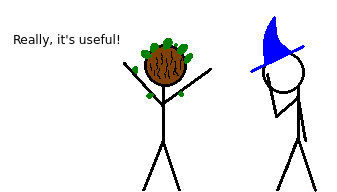
\includegraphics{Pics/Barkskin.png}
\end{figure*}

Barkskin grants a +2 enhancement bonus to the creature's existing natural armor bonus.

The enhancement bonus provided by barkskin stacks with the target's natural armor bonus, but not with other enhancement bonuses to natural armor. A creature without natural armor has an effective natural armor bonus of +0.

\paragraph{Augment:} For every 2 additional spell points you spend, the enhancement bonus to the creature's natural armor increases by 1.
\subsubsection{Bestow Curse}
\label{Spell:BestowCurse}
Necromancy
\\ \textbf{Level:} Blackguard 4, Evil 3, Luck 3, Sor/Wiz 4
\\ \textbf{Components:} V, S
\\ \textbf{Casting Time:} 1 standard action
\\ \textbf{Range:} Touch
\\ \textbf{Target:} Creature touched
\\ \textbf{Duration:} Permanent (D)
\\ \textbf{Saving Throw:} Will negates
\\ \textbf{Spell Resistance:} Yes
\\ \textbf{Spell Points:} Blackguard 7, Evil 5, Luck 5, Sor/Wiz 7

\emph{''A pox upon you! A POX!``}

You place a curse on the subject. Choose one of the following three effects.
\begin{list}{\labelitemi}{\leftmargin=1em}
 \item -6 decrease to an ability score (minimum 1).
 \item -4 penalty on attack rolls, saves, ability checks, and skill checks.
 \item Each turn, the target has a 50\% chance to act normally; otherwise, it takes no action.
\end{list}
The GM may add additional, more unique options to this spell, 
but they should be no more powerful than those described above (particularly when it comes to in-combat applications).

The curse bestowed by this spell cannot be dispelled, but it can be removed with a \nameref{Spell:LimitedWish}, \nameref{Spell:Miracle}, \nameref{Spell:RemoveCurse}, or \nameref{Spell:Wish} spell.

\paragraph{Augment:} If you spend an additional 6 spell points, you can select from a different menu of options:
\begin{enumerate}
 \item One of the subject's ability scores are reduced to 1.
 \item -8 penalty on attack rolls, saves, ability checks, and skill checks.
 \item Each turn, the target has a 25\% chance to act normally; otherwise, it takes no action.
\end{enumerate}
\subsubsection{Binding}
\label{Spell:Binding}
Enchantment (Compulsion) [Mind-Affecting]
\\ \textbf{Level:} Sor/Wiz 8 
\\ \textbf{Components:} V, S 
\\ \textbf{Casting Time:} One minute 
\\ \textbf{Range:} Close (25 ft. + 5 ft./2 levels)
\\ \textbf{Target:} One living creature 
\\ \textbf{Duration:} See text (D)
\\ \textbf{Saving Throw:} Will negates; see text
\\ \textbf{Spell Resistance:} Yes
\\ \textbf{Spell Points:} 15, XP

\emph{''And you shall remain this way until the king's castle is raised above the clouds!``}

A binding spell creates a magical restraint to hold a creature. 
The target gets an initial saving throw only if its Hit Dice equal at least one-half your caster level.

% You may have as many as six assistants help you with the spell. 
% For each assistant who casts suggestion, your caster level for this casting of binding increases by 1. 
% For each assistant who casts dominate animal, dominate person, or dominate monster, 
% your caster level for this casting of binding increases by a number equal to one-third of that assistant's level, 
% provided that the spell's target is appropriate for a binding spell. 
% Since the assistants' spells are cast simply to improve your caster level for the purpose of the binding spell, 
% saving throws and spell resistance against the assistants' spells are irrelevant. 
% Your caster level determines whether the target gets an initial Will saving throw and how long the binding lasts. 
All binding spells are dismissible.

Regardless of the version of binding you cast, 
you can specify triggering conditions that end the spell and release the creature whenever they occur. 
These triggers can be as simple or elaborate as you desire, but the condition must be reasonable and have a likelihood of coming to pass. 
The conditions can be based on a creature's name, identity, or alignment but otherwise must be based on observable actions or qualities. 
Intangibles such as level, class, Hit Dice, or hit points don't qualify. 
Once the spell is cast, its triggering conditions cannot be changed. 
Setting a release condition increases the save DC (assuming a saving throw is allowed) by 2.

If you are casting any of the first three versions of binding (those with limited durations), 
you may cast additional binding spells to prolong the effect, since the durations overlap. 
If you do so, the target gets a saving throw at the end of the first spell's duration, 
even if your caster level was high enough to disallow an initial saving throw. 
If the creature succeeds on this save, all the binding spells it has received are broken.

The binding spell has six versions. Choose one of the following versions when you cast the spell.
\begin{list}{\labelitemi}{\leftmargin=1em}
 \item \emph{Chaining:}
The subject is confined by restraints that generate an \nameref{Spell:TelepathicBeacon} spell (the repulsion version) affecting all creatures who approach the subject, except you. 
The duration is one year per caster level. 
The subject of this form of binding is confined to the spot it occupied when it received the spell.
\item \emph{Slumber:}
This version causes the subject to become comatose for as long as one year per caster level. 
The subject does not need to eat or drink while slumbering, nor does it age. 
This form of binding is more difficult to cast than chaining, making it slightly easier to resist. Reduce the spell's save DC by 1.
 \item \emph{Bound Slumber:}
This combination of chaining and slumber lasts for as long as one month per caster level. Reduce the save DC by 2.
 \item \emph{Hedged Prison:}
The subject is transported to or otherwise brought within a confined area from which it cannot wander by any means. 
The effect is permanent. Reduce the save DC by 3.
 \item \emph{Metamorphosis:}
The subject assumes gaseous form, except for its head or face. 
It is held harmless in a jar or other container, which may be transparent if you so choose. 
The creature remains aware of its surroundings and can speak, but it cannot leave the container, attack, or use any of its powers or abilities. 
The binding is permanent. 
The subject does not need to breathe, eat, or drink while metamorphosed, nor does it age. Reduce the save DC by 4.
 \item \emph{Minimus Containment:}
The subject is shrunk to a height of 1 inch or even less and held within some gem, jar, or similar object. 
The binding is permanent. The subject does not need to breathe, eat, or drink while contained, nor does it age. Reduce the save DC by 4.
\end{list}
You can't dispel a binding spell with \nameref{Spell:DispelMagic} or a similar effect, 
though an \nameref{Spell:AntimagicField} field or \nameref{Spell:Disjunction} affects it normally. 
A bound extraplanar creature cannot be sent back to its home plane due to dismissal, banishment, or a similar effect.

You must have specially made props suited to the specific type of binding at hand when you cast the spell.

\emph{Experience cost:} 100 XP + 100 XP per HD of the creature to be bound.
\subsubsection{Blackfire}
\label{Spell:Blackfire}
Evocation
\\ \textbf{Level:} Assassin 1, Blackguard 1
\\ \textbf{Components:} V, S
\\ \textbf{Casting Time:} 1 standard action
\\ \textbf{Range:} Medium (100 ft. + 10 ft./level)
\\ \textbf{Targets:} Up to one source of light/level
\\ \textbf{Duration:} 1 round/level (D)
\\ \textbf{Saving Throw:} Will negates (object); see text
\\ \textbf{Spell Resistance:} Yes (object); see text
\\ \textbf{Spell Points:} 1

\emph{The fires turn black, but continue to shed their light... at least as far as you are concerned.}

The light emitted by the targeted light sources changes in nature.
For you, the light sources shed light as brightly as ever before, but as far as anyone else is concerned, their light has completely vanished.

Secondary characteristics of the light sources remain unaffected, fires still are still hot, glowing magic weapons are still magic weapons, and so forth, but they no longer illuminate their surroundings for anyone but you.

You can target covered fires, such as those of lanterns. If a targeted source of fire sets another object on fire, the new object sheds light normally.

\paragraph{Augment:} You can augment this spell in one or both of the following ways:
\begin{enumerate}
 \item If you spend 2 additional spell points, this spell's duration increases to 10 minutes per level.
 \item For every 2 additional spell points you spend, you may designate one creature that shares your ability to see by the affected light sources.
\end{enumerate}
\subsubsection{Black Tentacles}
\label{Spell:BlackTentacles}
Conjuration (Creation)
\\ \textbf{Level:} Conjurer 4
\\ \textbf{Components:} V, S
\\ \textbf{Casting Time:} 1 standard action
\\ \textbf{Range:} Medium (100 ft. + 10 ft./level)
\\ \textbf{Area:} 20-ft.-radius spread
\\ \textbf{Duration:} 1 round/level (D)
\\ \textbf{Saving Throw:} None
\\ \textbf{Spell Resistance:} No
\\ \textbf{Spell Points:} 7

\emph{''The horror... the horror!``}

This spell conjures a field of rubbery black tentacles, each 10 feet long. 
These waving members seem to spring forth from the earth, floor, or whatever surface is underfoot (including water). 
They grasp and entwine around creatures that enter the area, holding them fast and crushing them with great strength.

Every creature within the area of the spell must make a grapple check, opposed by the grapple check of the tentacles. 
Treat the tentacles attacking a particular target as a Large creature with a base attack bonus equal to your caster level and a Strength score of 19. 
Thus, its grapple check modifier is equal to your caster level +8. 
The tentacles are immune to all types of damage.

Once the tentacles grapple an opponent, they may make a grapple check each round on your turn to deal 1d6+4 points of bludgeoning damage. 
The tentacles continue to crush the opponent until the spell ends or the opponent escapes.

Any creature that enters the area of the spell is immediately attacked by the tentacles. 
Even creatures who aren't grappling with the tentacles may move through the area at only half normal speed.

\paragraph{Augment:} 
% You can augment this spell in one or both of the following ways:
% \begin{enumerate}
%  \item 
If you spend 2 additional spell points, the tentacles grow
\href{http://www.giantitp.com/comics/oots0020.html}{wicked spikes}. 
The damage dealt by the tentacles changes to piercing and slashing damage, and increases to 1d6 + your caster level.
%  \item If you spend 4 additional spell points, the tentacles' length increases to 15 feet, and they count as a huge
%  creature. This increases their grapple check modifier to your caster level +12.
% \end{enumerate}
\subsubsection{Blade of the Sun}
\label{Spell:BladeOfTheSun}
Evocation [Good, Light]
\\ \textbf{Level:} Paladin 2, Sun 2
\\ \textbf{Components:} V
\\ \textbf{Casting Time:} 1 swift action
\\ \textbf{Range:} Touch
\\ \textbf{Target:} Melee weapon touched
\\ \textbf{Duration:} 1 round
\\ \textbf{Saving Throw:} None
\\ \textbf{Spell Resistance:} No
\\ \textbf{Spell Points:} 3

\emph{As you raise your blade high, it begins to shine with the white-hot power of the sun.}

For the duration of the spell, the touched weapon gains the benefits of the \emph{Brilliant Energy} weapon enhancement in addition to any other enchancements it may already have.
The weapon also shines bright light out to a 40' radius, and dim light another 40' beyond that. 
Even after the spell ends, the weapon sheds light as a torch for 1 round.

Casting this spell on a weapon that already has the Brilliant Energy enhancement has no additional effects, 
except with respect to the lighting and interaction with \nameref{Spell:DispelMagic} and similar effects.
\subsubsection{Blade Barrier}
\label{Spell:BladeBarrier}
Evocation [Force]
\\ \textbf{Level:} Good 6, War 6
\\ \textbf{Components:} V, S
\\ \textbf{Casting Time:} 1 standard action
\\ \textbf{Range:} Medium (100 ft. + 10 ft./level)
\\ \textbf{Effect:} Wall of whirling blades up to 20 ft. long/level, or a ringed wall of whirling blades with a radius of up to 5 ft. per two levels; either form 20 ft. high
\\ \textbf{Duration:} 1 min./level (D)
\\ \textbf{Saving Throw:} None or Reflex negates; see text
\\ \textbf{Spell Resistance:} Yes
\\ \textbf{Spell Points:} 11

\emph{An immobile, vertical curtain of whirling blades shaped of pure force springs into existence.}

Any creature passing through the wall you conjure takes 11d6 points of force damage, with no saving throw.
If you evoke the barrier so that it appears where creatures are, 
each creature takes damage as if passing through the wall, but each such creature can avoid the wall
(ending up on the side of its choice) and thus take no damage by making a successful Reflex save.
A blade barrier provides cover (+4 bonus to AC, +2 bonus on Reflex saves) against attacks made through it.

\paragraph{Augment:} Every additional spell point spent on this spell increases its damage by one die (d6).

\subsubsection{Bleed}
\label{Spell:Bleed}
Necromancy
\\ \textbf{Level:} Destruction 1
\\ \textbf{Components:} V, S
\\ \textbf{Casting Time:} 1 standard action
\\ \textbf{Range:} Touch
\\ \textbf{Target:} One living creature
\\ \textbf{Duration:} Instantaneous
\\ \textbf{Saving Throw:} Fortitude half
\\ \textbf{Spell Resistance:} Yes
\\ \textbf{Spell Points:} 1

\emph{The subject suddenly begins bleeding from every orifice.}

The target takes 1d3 points of Constitution damage. A successful Fortitude save reduces the Constitution damage by half (half of one point of damage is no damage).

\paragraph{Augment:} For every 3 additional spell points you spend, this spell's Constitution damage increases by one die (d3).
\subsubsection{Bless}
\label{Spell:Bless}
Enchantment (Compulsion) [Good, Mind-Affecting]
\\ \textbf{Level:} Good 1, Luck 1, Paladin 1
\\ \textbf{Components:} V, S
\\ \textbf{Casting Time:} 1 standard action
\\ \textbf{Range:} 40 ft.
\\ \textbf{Area:} All allies within a 40-ft. radius burst centered on you
\\ \textbf{Duration:} 1 round/level
\\ \textbf{Saving Throw:} None
\\ \textbf{Spell Resistance:} Yes
\\ \textbf{Spell Points:} 1

\emph{You bring special favor upon yourself and your allies while bringing disfavor to your enemies.}

You and your each of your allies gain a +1 luck bonus on attack rolls and saves vs. fear.

\paragraph{Augment:} You can Augment the spell in one or more of the following ways:
\begin{enumerate}
 \item If you spend 2 additional spell points, the luck bonus applies to all saving throws (not just saves vs. fear),
 weapon damage rolls, and skill checks, in addition to attack rolls.
 \item If you spend 2 additional spell points, this spell affects enemies as well as allies within the area.
 Enemies affected by the spell take a penalty on the appropriate rolls equal to the luck bonus provided to your allies.
 \item For every 6 additional power points you spend, the luck bonus gained on the appropriate rolls increases by 1.
 \item If you spend 1 additional spell point, this spell's duration increases to one minute per level.
\end{enumerate}
\subsubsection{Bless Weapon}
\label{Spell:BlessWeapon}
Transmutation
\\ \textbf{Level:} Paladin 1
\\ \textbf{Components:} V, S
\\ \textbf{Casting Time:} 1 standard action
\\ \textbf{Range:} Touch
\\ \textbf{Target:} Weapon touched
\\ \textbf{Duration:} 1 min./level
\\ \textbf{Saving Throw:} None
\\ \textbf{Spell Resistance:} No
\\ \textbf{Spell Points:} 1

\emph{Your weapon strikes true against evil foes.}

The transmuted weapon is treated as being magical for the purpose of bypassing the damage reduction of evil creatures or striking evil incorporeal creatures (though the spell doesn't grant an actual enhancement bonus). 
The weapon also becomes good, which means it can bypass the damage reduction of certain creatures. 
(This effect overrides and suppresses any other alignment the weapon might have.) 
Individual arrows or bolts can be transmuted, but affected projectile weapons (such as bows) don't confer the benefit to the projectiles they shoot.

In addition, all critical hit rolls against evil foes are automatically successful, so every threat is a critical hit. 
This last effect does not apply to any weapon that already has a magical effect related to critical hits, such as a keen weapon or a vorpal sword.
\subsubsection{Blight}
\label{Spell:Blight}
Necromancy [Death, Evil]
\\ \textbf{Level:} Death 4, Sor/Wiz 5
\\ \textbf{Range:} Touch
\\ \textbf{Target:} Plant creature touched, or plant touched; see text
\\ \textbf{Spell Points:} Death 7, Sor/Wiz 9

\emph{The plant withers and dies.}

This spell functions like the \nameref{Spell:DeathKnell} spell (including Augmentation options), 
except as outlined below.

Rather than targeting a creature with -1 or fewer hit points, it targets a plant creature with any number of HP remaining.

Plants that are not creatures (most are not) can still be targeted and killed by this spell,
but they provide you with no bonuses (just like killing creatures that do not have a full HD).
Such a mundane plant receives no saving throw against this spell, it simply withers and dies,
regardless of health and size.
\subsubsection{Blindness}
\label{Spell:Blindness}
Necromancy
\\ \textbf{Level:} Blackguard 2, Evil 2, Sor/Wiz 2
\\ \textbf{Components:} V
\\ \textbf{Casting Time:} 1 standard action
\\ \textbf{Range:} Medium (100 ft. + 10 ft./level)
\\ \textbf{Target:} One living creature
\\ \textbf{Duration:} Permanent (D)
\\ \textbf{Saving Throw:} Fortitude negates
\\ \textbf{Spell Resistance:} Yes
\\ \textbf{Spell Points:} 3

\emph{''My eyes! MY EYES!``}

You call upon the powers of unlife to render one of the subject's primary senses useless.
The subject becomes \emph{blind} or \emph{deaf}, or loses one special sense it may have (such as scent, blindsight, blindsense, or tremorsense). 

The name of the spell stems from its most common usage, as most humanoids rely on their sight more than any other sense.
\subsubsection{Blindsense}
\label{Spell:Blindsense}
Divination
\\ \textbf{Level:} Assassin 3, Sor/Wiz 3
\\ \textbf{Components:} V, S
\\ \textbf{Casting Time:} 1 standard action
\\ \textbf{Range:} Touch
\\ \textbf{Target:} Creature touched
\\ \textbf{Duration:} 1 min/level
\\ \textbf{Saving Throw:} Will negates (harmless)
\\ \textbf{Spell Resistance:} Yes (harmless)
\\ \textbf{Spell Points:} 3

\emph{Your senses widen, revealing things that were once hidden.}

The subject of this spell gains Blindsense out to 30'. 

\paragraph{Augment:} You can Augment the spell in one or both of the following ways:
\begin{enumerate}
 \item For every additional spell point you spend, the range of the blindsense increases by 10'.
 \item If you spend two additional spell points, the spell's dueation increases to 10 minutes per level.
\end{enumerate}

\subsubsection{Blink}
\label{Spell:Blink}
Conjuration (Teleportation)
\\ \textbf{Level:} Bard 3, Sor/Wiz 3
\\ \textbf{Components:} V, S
\\ \textbf{Casting Time:} 1 standard action
\\ \textbf{Range:} Touch
\\ \textbf{Target:} Creature touched
\\ \textbf{Duration:} 1 round/level (D)
\\ \textbf{Spell Points:} 5

\emph{The creature vanishes and reappears at a maddening rate.}

The subject ``blinks`` back and forth between the Material Plane and the Ethereal Plane, spending
roughly half his time on the Material Plane and half on the Ethereal Plane. 
He looks as though he's winking in and out of reality very quickly and at random
(the blinking can be controlled by neither the caster nor the subject).

Blinking has several effects on an opponent's chance to hit, as follows\footnote{
Blink effectively grants two ''different'' miss chances, although it may not be immediately obvious
(one for being simply not there half the time, the other half for not being visible all the time.
This means the spell has complicated interactions with other spells that grant similar benefits. 
Those who intend to use this spell in conjunction with others may want to spend time reading the spell descriptions thoroughly.
% For example:
% \begin{list}{\labelitemi}{\leftmargin=1em}
%  \item Blur + Blink: The miss chance granted by \nameref{Spell:Blur}
%  overlaps with the ``not visible'' (concealment) 
%  aspect of Blink, combined they only grant a 20\% miss chance, 
%  or a 50\% miss chance if the Blur spell is Augmented. STUFFSTUFFSTUFF
%  \item Invisibility + Blink: The miss chance granted by \nameref{Spell:Invisibility}
%  overlaps with the ``not visible'' (concealment) 
%  aspect of Blink, combined they only grant a 50\% miss chance. STUFFSTUFFSTUFF
% \end{list}
}:

\begin{list}{\labelitemi}{\leftmargin=1em}
 \item Physical attacks against the subject have a 50\% miss chance. 
 The Blind-Fight feat doesn't help opponents, since he is ethereal and not merely invisible.
 \item If the attacker is capable of striking ethereal creatures, but not \emph{seeing}
 ethereal creatures, the miss chance is only 20\% (for limited concealment).
 The miss chance is less than that offered by true invisibility, because the subject of the spell
 is perfectly visible half the time.
 \item If the attacker can see ethereal creatures, the miss chance is also only 20\%.
 This is because even though the attacker can't hit the subject while he is ethereal, 
 attacks can be timed to mostly hit while the subject is on the material plane.
 \item For an attacker that can both see and strike ethereal creatures, there is no miss chance.
\end{list}  
Likewise, your own attacks have a 20\% miss chance, 
since you sometimes go ethereal just as you are about to strike.

Any individually targeted spell has a 50\% chance to fail against you while you're blinking unless 
your attacker can target invisible, ethereal creatures. 
Your own spells have a 20\% chance to activate just as you go ethereal, 
in which case they typically do not affect the Material Plane.

While blinking, you take only half damage from area attacks 
(but full damage from those that extend onto the Ethereal Plane). 
You strike as an invisible creature (with a +2 bonus on attack rolls), 
denying your target any Dexterity bonus to AC.

You take only half damage from falling, since you fall only while you are material.

While blinking, you can step through (but not see through) solid objects. 
For each 5 feet of solid material you walk through, 
there is a 50\% chance that you become material. 
If this occurs, you are shunted off to the nearest open space and take 1d6 points of damage per 5 feet so traveled. 
You can move at only three-quarters speed 
(because movement on the Ethereal Plane is at half speed, 
and you spend about half your time there and half your time material.)

Since you spend about half your time on the Ethereal Plane, 
you can see and even attack ethereal creatures. 
You interact with ethereal creatures roughly the same way you interact with material ones.

An ethereal creature is invisible, incorporeal, 
and capable of moving in any direction, even up or down. 
As an incorporeal creature, you can move through solid objects, including living creatures.

An ethereal creature can see and hear the Material Plane, 
but everything looks gray and insubstantial. 
Sight and hearing on the Material Plane are limited to 60 feet.

Force effects and abjurations affect you normally. 
Their effects extend onto the Ethereal Plane from the Material Plane, but not vice versa. 
An ethereal creature can't attack material creatures, 
and spells you cast while ethereal affect only other ethereal things. 
Certain material creatures or objects have attacks or effects that work on the Ethereal Plane. 
Treat other ethereal creatures and objects as material.

\paragraph{Augment:} If you spend 4 additional spell points, the subject can perfectly predict its own blinking,
although it still cannot control it. This negates the 20\% effective miss chance the subject suffers on attacks, as
well as the chance of its spells accidentally going off on the ethereal plane.
\subsubsection{Bloodhound}
\label{Spell:Bloodhound}
Transmutation
\\ \textbf{Level:} Ranger 1
\\ \textbf{Components:} V, S
\\ \textbf{Casting Time:} 1 standard action
\\ \textbf{Range:} Touch
\\ \textbf{Target:} Creature touched
\\ \textbf{Duration:} 10 min./level
\\ \textbf{Saving Throw:} None
\\ \textbf{Spell Resistance:} Yes (harmless)

\emph{``Your nose twitches, and the world gains a whole new dimension.''}

The subject gains the scent special ability, and a +2 enhancement bonus on Survival checks when tracking.

\paragraph{Augment:} For every additional spell point you spend, this spell's enhancement bonus on Survival checks increases by 1.
\subsubsection{Bloodletting Arrow}
\label{Spell:BloodlettingArrow}
Transmutation
\\ \textbf{Level:} Ranger 3
\\ \textbf{Components:} V
\\ \textbf{Casting Time:} 1 swift action
\\ \textbf{Range:} Touch
\\ \textbf{Target:} One arrow or bolt touched
\\ \textbf{Duration:} Until end of round; see text
\\ \textbf{Saving Throw:} None, Fort half; see text
\\ \textbf{Spell Resistance:} No
\\ \textbf{Spell Points:} 5

\emph{Blood pours out of the wound inflicted by your arrow like a stream.}

A creature struck by the projectile takes 1d6 points of Constitution damage.
A successful Fortitude save reduces the Constitution damage by half.
The projectile remains so enhanced only until the end of the current turn. 
If the projectile does not hit a creature before the end of the turn, the spell drains away harmlessly.

\paragraph{Augment:} For every 6 additional spell points you spend, this spell deals an additional 1d6 points of Constitution damage.
\subsubsection{Blur}
\label{Spell:Blur}
Illusion (Glamer)
\\ \textbf{Level:} Sor/Wiz 2
\\ \textbf{Components:} V
\\ \textbf{Casting Time:} 1 standard action
\\ \textbf{Range:} Touch
\\ \textbf{Target:} Creature touched
\\ \textbf{Duration:} 1 round./level (D)
\\ \textbf{Saving Throw:} Will negates (harmless)
\\ \textbf{Spell Resistance:} Yes (harmless)
\\ \textbf{Spell Points:} 3

\emph{The subject's outline appears blurred, shifting and wavering.}

The glamer grants the subject concealment (20\% miss chance).

A \nameref{Spell:SeeInvisibility} spell does not counteract the blur effect, but a \nameref{Spell:TrueSeeing} spell does.

\paragraph{Augment:} You can augment this spell in one or both of the following ways:
\begin{enumerate}
 \item If you spend 4 additional spell points, the creature benefits from a 50\% miss chance as if it had total concealment. 
However, unlike actual total concealment, this augment does not prevent enemies from targeting the creature normally.
 \item If you spend 2 additional spell points, the spell's duration increases to one minute per level.
\end{enumerate}
\subsubsection{Body of Light}
\label{Spell:BodyOfLight}
Transmutation (Polymorph) [Light]
\\ \textbf{Level:} Paladin 4, Sun 5
\\ \textbf{Components:} V,S
\\ \textbf{Casting Time:} 1 standard action
\\ \textbf{Range:} Touch
\\ \textbf{Target:} Willing living creature touched
\\ \textbf{Duration:} 1 min./level (D)
\\ \textbf{Saving Throw:} None
\\ \textbf{Spell Resistance:} No
\\ \textbf{Spell Points:} Paladin 7, Sun 9

\emph{The creature's skin glows with an intense, pure light, as if constructed of it.}

The creature's skin and flesh is changed into pure light, granting it immunity to poison, sleep effects, paralysis, stunning, critical hits, and flanking.

In addition, the creature's skin sheds light as bright as full daylight in a 60-foot radius, and dim light for an additional 60 feet beyond that. 

If an area of magical light and an area of magical darkness overlap, 
the spell on which more spell points were spent prevails.
If an equal number of spell points were spent on both spells, ambient light conditions remain.

\paragraph{Augment:} If you spend 4 additional spell points, the creature is able to retain more of itself throughout the transformation.
The creature retains all its class features when polymorphed (notably, allowing spellcasting).
This is an exception to the general rules of Polymorph subschool spells.
\subsubsection{Bow of the Solar}
\label{Spell:BowOfTheSolar}
Necromancy [Death, Good]
\\ \textbf{Level:} Paladin 6
\\ \textbf{Components:} V, S
\\ \textbf{Casting Time:} 1 standard action
\\ \textbf{Range:} Long (400 ft. + 40 ft./level)
\\ \textbf{Effect:} Ray
\\ \textbf{Duration:} Instantaneous
\\ \textbf{Saving Throw:} Fortitude negates
\\ \textbf{Spell Resistance:} Yes
\\ \textbf{Spell Points:} 11

\emph{A great, partially translucent bow appears in your hands, lasting just long enough for you to fire a single arrow.}

You must succeed on a ranged touch attack to hit your opponent.
On a hit, the opponent must succeed on a Fortitude saving throw or be instantly slain.
An evil creature takes a -4 penalty on the save.
If the save is successful, the creature instead takes damage as if struck by a +2 arrow shot from a composite longbow sized for you, including your full strength modifier and all other situational modifiers that may apply.
\subsubsection{Burn}
\label{Spell:Burn}
Evocation [Fire]
\\ \textbf{Level:} Evoker 1
\\ \textbf{Components:} V, S
\\ \textbf{Casting Time:} 1 standard action
\\ \textbf{Range:} Close (25 ft. + 5 ft./2 levels)
\\ \textbf{Target:} One creature; see text
\\ \textbf{Duration:} 5 rounds
\\ \textbf{Saving Throw:} None, Reflex negates; See text
\\ \textbf{Spell Resistance:} Yes
\\ \textbf{Spell Points:} 1

\emph{``Do you remember the time when you said I was a nerd for going to Wizarding school? NOW BURN FOR IT!''}

A creature that takes fire damage while this spell is in effect magically catches on fire.
One round after catching on fire, and once per round thereafter, the spell deals additional fire damage equal to one-half the fire damage that set it on fire in the first place.
If a creature takes fire damage multiple times while the spell lasts, use one-half of the largest damage value.

\paragraph{Augment:} For every additional spell point you spend, this spell lasts for an additional round.
\subsection{'C' Spells}
\subsubsection{Call Lightning}
\label{Spell:CallLightning}
Evocation [Electricity]
\\ \textbf{Level:} Air 3, Destruction 3
\\ \textbf{Components:} V, S
\\ \textbf{Casting Time:} 1 standard action
\\ \textbf{Range:} Medium (100 ft. + 10 ft./level)
\\ \textbf{Effect:} One or more 30-ft.-long vertical lines of lightning
\\ \textbf{Duration:} 1 min./level
\\ \textbf{Saving Throw:} Reflex half
\\ \textbf{Spell Resistance:} Yes
\\ \textbf{Spell Points:} 5

\emph{You call bolts of lightning out from the air to strike your enemies.}

Immediately upon completion of the spell, and once per round thereafter, you may call down a 5-foot-wide, 30-foot-long, vertical bolt of lightning that deals 3d6 points of electricity damage. 
The bolt of lightning flashes down in a vertical stroke at whatever target point you choose within the spell's range (measured from your position at the time). 
Any creature in the target square or in the path of the bolt is affected.

You need not call a bolt of lightning immediately; other actions, even spellcasting, can be performed. 
However, each round after the first you may use a standard action (concentrating on the spell) to call a bolt. You may call a total number of five bolts.

If you are outdoors and in a stormy area - a rain shower, clouds and wind, hot and cloudy conditions, or even a tornado (including a whirlwind formed by a djinni or an air elemental of at least Large size) - each bolt deals 3d10 points of electricity damage instead of 3d6.

This spell functions indoors or underground but not underwater.

\paragraph{Augment:} For every 2 additional spell points you spend, this spell's damage increases by one die (d6 or d10).

In addition, for every additional spell point you spend, you may call down an additional bolt.
\subsubsection{Calm Emotions}
\label{Spell:CalmEmotions}
Enchantment (Compulsion) [Mind-Affecting]
\\ \textbf{Level:} Law 2
\\ \textbf{Components:} V, S
\\ \textbf{Casting Time:} 1 standard action
\\ \textbf{Range:} Medium (100 ft. + 10 ft./level)
\\ \textbf{Area:} Creatures in a 20-ft.-radius spread
\\ \textbf{Duration:} Concentration, up to 1 round/level
\\ \textbf{Saving Throw:} Will negates
\\ \textbf{Spell Resistance:} Yes
\\ \textbf{Spell Points:} 3

\emph{``Be at ease.''}

This spell calms agitated creatures. 
You have no control over the affected creatures, but calm emotions can stop raging creatures from fighting or joyous ones from reveling. 
Creatures so affected cannot take violent actions (although they can defend themselves) or do anything destructive. 
Any aggressive action against or damage dealt to a calmed creature immediately breaks the spell on all calmed creatures.

This spell automatically suppresses (but does not dispel) any morale bonuses granted by spells such as \nameref{Spell:Bless} or \nameref{Spell:Rage}, 
as well as negating a bard's ability to inspire courage or a barbarian's rage ability. 

It also suppresses any fear effects and removes the confused condition from all targets. 
While the spell lasts, a suppressed spell or effect has no effect. 
When the calm emotions spell ends, the original spell or effect takes hold of the creature again, provided that its duration has not expired in the meantime.

\paragraph{Augment:} If you spend 4 additional spell points, this spell's duration changes to 1 round/level (D).
\subsubsection{Celestial Flight}
\label{Spell:CelestialFlight}
Transmutation [Good]
\\ \textbf{Level:} Paladin 3

\emph{The subject grows great, white, angelic wings.}

This spell functions as the \nameref{Spell:Fly} spell (including its augmentation option), except as noted here, and that the flight is due to physical wings the subject grows (which matters for effects like those cause by tanglefoot bags).
\subsubsection{Charm}
\label{Spell:Charm}
Enchantment (Charm) [Mind-Affecting]
\\ \textbf{Level:} Bard 1, Enchanter 1
\\ \textbf{Components:} V, S
\\ \textbf{Casting Time:} 1 standard action
\\ \textbf{Range:} Close (25 ft. + 5 ft./2 levels)
\\ \textbf{Target:} One humanoid
\\ \textbf{Duration:} 1 hour/level
\\ \textbf{Saving Throw:} Will negates
\\ \textbf{Spell Resistance:} Yes
\\ \textbf{Spell Points:} 1

\emph{``Look at me. Look! You remember me, right?''}

This charm makes a humanoid creature regard you as its trusted friend and ally (treat the target's attitude as friendly). 
If the creature is currently being threatened or attacked by you or your allies, however, it receives a +5 bonus on its saving throw.

The spell does not enable you to control the charmed person as if it were an automaton, 
but it perceives your words and actions in the most favorable way. You can try to give the subject orders, 
but you must win an opposed Charisma check to convince it to do anything it wouldn't ordinarily do. 
(Retries are not allowed.) An affected creature never obeys suicidal or obviously harmful orders, 
but it might be convinced that something very dangerous is worth doing. 
Any act by you or your apparent allies that threatens the charmed person breaks the spell. 
You must speak the person's language to communicate your commands, or else be good at pantomiming.

\paragraph{Augment:} You can augment this spell in one or more of the following ways.
\begin{enumerate}
 \item If you spend 2 additional spell points, this spell can also affect an animal, fey, giant, magical beast, or monstrous humanoid.
 \item If you spend 6 additional spell points, this spell can also affect an aberration, dragon, elemental, or outsider in addition to the creature types mentioned above.
 \item If you spend 4 additional spell points, this spell's duration increases to one day per level.
 \item For every 3 additional spell points you spend, this spell can affect an additional target. 
No target of the spell can be more than 15 feet from another target of the spell.
\end{enumerate}
%In addition, for every 2 additional spell points you spend to achieve any of these effects, this spell's save DC increases by 1.

\subsubsection{Chain Lightning}
\label{Spell:ChainLightning}
Evocation [see text]
\\ \textbf{Level:} Air 6, Evoker 6
\\ \textbf{Components:} V, S
\\ \textbf{Casting Time:} 1 standard action
\\ \textbf{Range:} Long (400 ft. + 40 ft./level)
\\ \textbf{Target:} One primary target, plus ten secondary targets (each of which must be within 30 ft. of the primary target)
\\ \textbf{Duration:} Instantaneous
\\ \textbf{Saving Throw:} Reflex Half
\\ \textbf{Spell Resistance:} Yes
\\ \textbf{Spell Points:} 11

\emph{A discharge of energy explodes from your fingertips towards the monster, and from that monster to the next, and on until the whole group is howling in pain.}

The arc of energy unerringly strikes one creature or object within range, then arcs to up to 10 other targets.
You choose an energy type at the time of casting.

Every target hit by the arc takes 11d6 points of damage, but can attempt a Reflex saving throw for half damage. 

You choose secondary targets as you like, but they must all be within 30 feet of the primary target, and no target can be struck more than once. 
You can choose to affect fewer secondary targets than the maximum.

The name of the spell refers to the lightning form of the spell.
Causing electrical energy to arc between targets is considered more intuitive than doing the same trick with other energy types according to most spellcasters, resulting in that form being the one being most quickly mastered by most.
\begin{list}{\labelitemi}{\leftmargin=1em}
 \item Cold: An arc of this energy type deals +1 point of damage per die. 
 The saving throw to reduce damage from a cold arc is a Fortitude save instead of a Reflex save.
 \item Electricity: An arc of this energy type provides a +2 bonus to the save DC
 and a +2 bonus on caster level checks for the purpose of overcoming spell resistance.
 \item Fire: An arc of this energy type deals +1 point of damage per die.
 \item Sonic: An arc of this energy type deals -1 point of damage per die and ignores an object's hardness.
\end{list}
This spell's descriptor is the same as the type of energy you selected. 

\paragraph{Augment:} For every additional spell point you spend, 
this spell's damage increases by one die (d6), and you can select an additional secondary target.
% \subsubsection{Chill Touch}
% \label{Spell:ChillTouch}
% Necromancy
% \\ \textbf{Level:} Sor/Wiz 1
% \\ \textbf{Components:} V, S
% \\ \textbf{Casting Time:} 1 standard action
% \\ \textbf{Range:} Touch
% \\ \textbf{Targets:} Creature or creatures touched (up to one/level)
% \\ \textbf{Duration:} Instantaneous
% \\ \textbf{Saving Throw:} Fortitude partial or Will negates; see text
% \\ \textbf{Spell Resistance:} Yes
% \\ \textbf{Spell Points:} 1
% 
% A touch from your hand, which glows with blue energy, disrupts the life force of living creatures. 
% Each touch channels negative energy that deals 1d6 points of damage. 
% The touched creature also takes 1 point of Strength damage unless it makes a successful Fortitude saving throw. 
% You can use this melee touch attack up to one time per level.
% 
% An undead creature you touch takes no damage of either sort, 
% but it must make a successful Will saving throw or flee as if panicked for 1d4 rounds +1 round per caster level.
% 
% %\paragraph{Augment:} For every 2 additional spell points you spend, this spell's save DC increases by 1.

\subsubsection{Clairvoyance}
\label{Spell:Clairvoyance}
Divination (Scrying)
\\ \textbf{Level:} Assassin 3, Bard 3, Diviner 2, Knowledge 2
\\ \textbf{Components:} V, S
\\ \textbf{Casting Time:} 1 standard action
\\ \textbf{Range:} Unlimited
\\ \textbf{Effect:} Magical sensor
\\ \textbf{Duration:} 1 min./level (D)
\\ \textbf{Saving Throw:} None
\\ \textbf{Spell Resistance:} No
\\ \textbf{Spell Points:} Assassin 5, Diviner 3, Knowledge 3

\emph{You free your senses from your body, allowing them to spy on areas far away.}

You can see and hear a distant location almost as if you were there. 
You don't need line of sight or line of effect, but the locale must be known - 
a place familiar to you or an obvious one, such as behind a door, around a corner, or in a grove of trees. 
Once you have selected the locale, the magical sensor doesn't move, but you can rotate it in all directions to view the area as desired. 
Unlike other scrying spells, this spell does not allow magically or supernaturally enhanced senses to work through it.
If the chosen locale is magically dark, you see nothing. 
If it is naturally pitch black, 
you can see in a 10- foot radius around the center of the spell's effect (or, if you have natural darkvision, out to the extent of its range). 
Distance is not a factor, but the spell does not work across planes.

\subsubsection{Color Spray}
\label{Spell:ColorSpray}
Illusion (Pattern) [Mind-Affecting]
\\ \textbf{Level:} Sor/Wiz 1
\\ \textbf{Components:} V, S
\\ \textbf{Casting Time:} 1 standard action
\\ \textbf{Range:} 15 ft.
\\ \textbf{Area:} Cone-shaped burst
\\ \textbf{Duration:} Instantaneous; see text
\\ \textbf{Saving Throw:} Will negates
\\ \textbf{Spell Resistance:} Yes
\\ \textbf{Spell Points:} 1

\emph{A vivid cone of clashing colors springs forth from your hand.}

Creatures in the affected area are stunned for 1 round.
A successful Will save negates this effect.

Sightless creatures and creatures that are blind are not affected by color spray.

\paragraph{Augment:} Spending additional spell points on this spell allows it to have an overwhelming effect on weaker creatures.

\begin{enumerate}
\item Spending five or more spell points than the creature has HD means that on a failed save,
the creature is unconscious, blinded, and stunned for 2d4 rounds, then blinded and stunned for 1d4 rounds, and then stunned for 1 round. 
(Only living creatures are knocked unconscious.)
\item Spending three or more spell points than the creature has HD means that on a failed save, 
the creature is blinded and stunned for 1d4 rounds, and then stunned for 1 round. 
\end{enumerate}
%In addition, for every 2 additional spell points you spend, this spell's save DC increases by 1.
\subsubsection{Command}
\label{Spell:Command}
Enchantment (Compulsion) [Language-Dependent, Mind-Affecting]
\\ \textbf{Level:} Law 1
\\ \textbf{Components:} V
\\ \textbf{Casting Time:} 1 standard action
\\ \textbf{Range:} Close (25 ft. + 5 ft./2 levels)
\\ \textbf{Target:} One living creature
\\ \textbf{Duration:} 1 round
\\ \textbf{Saving Throw:} Will negates
\\ \textbf{Spell Resistance:} Yes
\\ \textbf{Spell Points:} 1

\emph{You imbue your voice with such power that creatures obey your commands before they can think to question your authority.}

You give the subject a single command, which it obeys to the best of its ability at its earliest opportunity. You may select from the following options.

\begin{list}{\labelitemi}{\leftmargin=1em}
 \item \emph{Approach:}
On its turn, the subject moves toward you as quickly and directly as possible for the spell's duration. 
The creature may do nothing but move during its turn, and it provokes attacks of opportunity for this movement as normal.
 \item \emph{Drop:}
On its turn, the subject drops whatever it is holding. 
It can't pick up any dropped item for the duration of the spell.
 \item \emph{Fall:}
On its turn, the subject falls to the ground and remains prone for the spell's duration. 
It may act normally while prone but takes any appropriate penalties.
 \item \emph{Flee:}
On its turn, the subject moves away from you as quickly as possible for the spell's duration. 
It may do nothing but move during its turn, and it provokes attacks of opportunity for this movement as normal.
 \item \emph{Halt:}
The subject stands in place for the spell's duration. 
It may not take any actions but is not considered helpless.
\end{list}
\paragraph{Augment:} For every 2 additional spell points you spend, this spell's duration increases by one round.
\subsubsection{Command Nature's Allies}
\label{Spell:CommandNaturesAllies}
Transmutation
\\ \textbf{Level:} Plant 2, Ranger 2
\\ \textbf{Targets:} One elemental, fey, or plant creature

\emph{``Run, forest, run!''}

This spell functions as \nameref{Spell:CommandUndead}, except as noted here.
\subsubsection{Command Undead}
\label{Spell:CommandUndead}
Necromancy
\\ \textbf{Level:} Blackguard 2, Death 2, Necromancer 2
\\ \textbf{Components:} V, S
\\ \textbf{Casting Time:} 1 standard action
\\ \textbf{Range:} Close (25 ft. + 5 ft./2 levels)
\\ \textbf{Targets:} One undead creature
\\ \textbf{Duration:} One day/level
\\ \textbf{Saving Throw:} Will negates; see text
\\ \textbf{Spell Resistance:} Yes
\\ \textbf{Spell Points:} 3

\emph{``Go forth, and make a feast of the flesh of the living!''}

This spell allows you some degree of control over an undead creature. 
Assuming the subject is intelligent, it perceives your words and actions in the most favorable way (treat its attitude as friendly). 
It will not attack you while the spell lasts. 
You can try to give the subject orders, but you must win an opposed Charisma check to convince it to do anything it wouldn't ordinarily do. (Retries are not allowed.) 
An intelligent commanded undead never obeys suicidal or obviously harmful orders, but it might be convinced that something very dangerous is worth doing.

A nonintelligent undead creature gets no saving throw against this spell. 
When you control a mindless being, you can communicate only basic commands, such as ``come here,`` ``go there,`` ``fight,'' ''stand still,`` and so on. 
Nonintelligent undead never resist orders, even suicidal or obviously harmful ones.

Any act by you or your apparent allies that threatens the commanded undead (regardless of its Intelligence) breaks the spell.

Your commands are not telepathic. The undead creature must be able to hear you.

%\paragraph{Augment:} For every 2 additional spell points you spend, this spell's save DC increases by 1.
\subsubsection{Commune}
\label{Spell:Commune}
Divination
\\ \textbf{Level:} Blackguard 5, Cleric 5, Paladin 5
\\ \textbf{Components:} V, S
\\ \textbf{Casting Time:} 10 minutes
\\ \textbf{Range:} Personal
\\ \textbf{Target:} You
\\ \textbf{Duration:} 1 round/level
\\ \textbf{Spell Points:} 9, XP

\emph{''Grant me wisdom in this hour of need.``}

You contact your patron deity - or agents thereof - and ask questions that can be answered by a simple yes or no. 
(A caster with no particular patron deity contacts a philosophically allied deity.) 
You are allowed three such questions. 
The answers given are correct within the limits of the entity's knowledge. 
''Unclear'' is a legitimate answer, because powerful beings of the Outer Planes are not necessarily omniscient. 
In cases where a one-word answer would be misleading or contrary to the deity's interests, 
a short phrase (five words or less) may be given as an answer instead.

The spell, at best, provides information to aid character decisions. 
The entities contacted structure their answers to further their own purposes. 
If you lag, discuss the answers, or go off to do anything else, the spell ends.

\paragraph{Augment:} For every 2 additional spell points you spend, 
you can ask an additional question.

\emph{Experience Cost:} 100 XP.

\subsubsection{Commune with Nature}
\label{Spell:CommuneWithNature}
Divination
\\ \textbf{Level:} Earth 5, Ranger 4
\\ \textbf{Components:} V, S
\\ \textbf{Casting Time:} 10 minutes
\\ \textbf{Range:} Personal
\\ \textbf{Target:} You
\\ \textbf{Duration:} Instantaneous
\\ \textbf{Spell Points:} Earth 9, Ranger 7

\emph{You become one with nature, attaining knowledge of the surrounding territory.} 

You instantly gain knowledge of as many as three facts from among the following subjects: the ground or terrain, plants, minerals, bodies of water, the presence and races of people, general animal population, presence of woodland creatures, presence of powerful unnatural creatures, the locations of nearby settlements (which show up as blanks in the spell's coverage) or even the general state of the natural setting.

In outdoor settings, the spell operates in a radius of 1 mile per caster level. 
In natural underground settings - caves, caverns, and the like - the radius is limited to 100 feet per caster level.

The spell does not function where nature has been replaced by construction or settlement, such as in dungeons and towns.

\paragraph{Augment:} If you spend 4 additional spell points, you can cast this spell as a standard action.
\subsubsection{Comprehend Languages}
\label{Spell:ComprehendLanguages}
Divination
\\ \textbf{Level:} Bard 1, Diviner 1, Knowledge 1
\\ \textbf{Components:} V, S
\\ \textbf{Casting Time:} 1 standard action
\\ \textbf{Range:} Personal
\\ \textbf{Target:} You
\\ \textbf{Duration:} 10 min./level (D)
\\ \textbf{Spell Points:} 1

\emph{Your mind widens, and what was incomprehensible only moments earlier is now clear as day.}

When casting this spell, select a single language you do not know. For the duration of the spell, you can understand and read (but not speak or write) that language.

%Comprehend languages can be made permanent with a permanency spell.

\paragraph{Augment:} You can augment this spell in one or more of the following ways.
\begin{enumerate}
 \item If you spend 2 additional spell points, you do not need to select a language when casting the spell, you gain knowledge of all languages.
 \item If you spend 4 additional spell points, you gain the ability to speak and write the language(s).
 \item If you spend 2 additional spell points, the range of the spell increases to touch, and the target changes to ''creature touched``.
 \item If you spend 8 additional spell points and 500XP, the spell's duration increases to Permanent.
\end{enumerate}
\subsubsection{Cone of Cold} 
\label{Spell:ConeOfCold}
Evocation [See text]
\\ \textbf{Level:} Evoker 5, Water 5
\\ \textbf{Components:} V, S
\\ \textbf{Casting Time:} 1 standard action
\\ \textbf{Range:} 60 ft.
\\ \textbf{Area:} Cone-shaped burst
\\ \textbf{Duration:} Instantaneous
\\ \textbf{Saving Throw:} Reflex partial, see text
\\ \textbf{Spell Resistance:} Yes
\\ \textbf{Spell Points:} 9

\emph{A blast of energy originates at your hand and extends outward in a cone.}

At the time of casting, you choose between cold, electricity, fire, or sonic damage.
All creatures in the area take 9d6 points of damage, and are \emph{slowed} (as if by the \nameref{Spell:Slow} spell) for one round.
A successful reflex save negates the slowing effect and halves the damage.

The name of the spell refers to the cold version of the spell, which was the form of the spell originally discovered.
Although other forms of the spell were later discovered, ''Cone of Cold'' remains as its name.
\begin{list}{\labelitemi}{\leftmargin=1em}
 \item Cold: A blast of this energy type deals +1 point of damage per die. 
 \item Electricity: A blast of this energy type provides a +2 bonus to the save DC
 and a +2 bonus on caster level checks for the purpose of overcoming spell resistance.
 \item Fire: A blast of this energy type deals +1 point of damage per die.
 The saving throw to reduce damage from a fire blast is a Fortitude save instead of a Reflex save.
 \item Sonic: A blast of this energy type deals -1 point of damage per die and ignores an object's hardness.
\end{list}

This spell's descriptor is the same as the type of energy you selected. 

\paragraph{Augment:} For every additional spell point you spend, 
this spell's damage increases by one die (d6).
\subsubsection{Confusion}
\label{Spell:Confusion}
Enchantment (Compulsion) [Mind-Affecting]
\\ \textbf{Level:} Bard 3, Sor/Wiz 4, Trickery 4
\\ \textbf{Components:} V, S
\\ \textbf{Casting Time:} 1 standard action
\\ \textbf{Range:} Medium (100 ft. + 10 ft./level)
\\ \textbf{Targets:} All creatures in a 15-ft. radius burst
\\ \textbf{Duration:} 1 round/level
\\ \textbf{Saving Throw:} Will negates
\\ \textbf{Spell Resistance:} Yes
\\ \textbf{Spell Points:} Bard 5, Sor/Wiz 7, Trickery 7

\emph{You stir the thoughts of your victims around until they can no longer tell thought from reality.}

This spell causes the targets to become \emph{confused}, making them unable to independently determine what they will do.

\paragraph{Augment:} If you spend 6 additional spell points, this spell's duration changes to permanent.
Creatures rendered permanently \emph{confused} in this way are referred to as insane.
\subsubsection{Consecrate}
\label{Spell:Consecrate}
Evocation [Good]
\\ \textbf{Level:} Good 2
\\ \textbf{Components:} V, S
\\ \textbf{Casting Time:} 1 standard action
\\ \textbf{Range:} Close (25 ft. + 5 ft./2 levels)
\\ \textbf{Area:} 20-ft.-radius emanation
\\ \textbf{Duration:} 2 hours/level
\\ \textbf{Saving Throw:} None
\\ \textbf{Spell Resistance:} Yes
\\ \textbf{Spell Points:} 3

\emph{You imbue the area with positive energy.}

Every undead creature entering a consecrated area takes a -1 penalty on attack rolls, damage rolls, and saving throws,
and gains a further -4 penalty on all saving throws against the \nameref{Feat:TurnUndead} feat.

Undead creatures cannot be summoned into or created within a consecrated area.
If the consecreted area contains an altar, shrine, or other permanent fixture dedicated to your deity or aligned higher power, 
the modifiers given above are doubled (-2 penalty on attack rolls, damage rolls, and saving throws, -8 penalty against being turned). 
If the area contains an altar, shrine, or other permanent fixture of a deity, pantheon, or higher power other than your
patron, the consecrate spell instead curses the area, cutting off its connection with the associated deity or power. 
This secondary function, if used, does not also grant the penalties relating to undead, as given above.

\paragraph{Augment:} If you spend 4 additional spell points, all non-evil creatures within the spell's area gain the benefits of the good-aligned version of the
\nameref{Spell:AlignedProtection} spell (also known as Protection from Evil).
\subsubsection{Contact Other Plane}
\label{Spell:ContactOtherPlane}
Divination
\\ \textbf{Level:} Diviner 5
\\ \textbf{Components:} V
\\ \textbf{Casting Time:} 10 minutes
\\ \textbf{Range:} Personal
\\ \textbf{Target:} You
\\ \textbf{Duration:} Instantaneous
\\ \textbf{Spell Points:} 9

\emph{You send your mind on a dangerous mental journey to another plane of existence in order to receive advice and information from powers there.}

When casting this spell, you attempt to ask a question of one of the great powers of the universe - a deity or even the incomprehensibly vast consciousness of a plane of existence.
See the \nameref{tab:ContactOtherPlane} table for possible consequences and results of the attempt, which includes the possibility of your intelligence and charisma temporarily decreasing.

The powers reply in a language you understand, but they resent being contacted in this manner and give only very brief answers to your questions
(All questions are answered with ''yes,'' ''no,'' ''maybe,'' ''never,'', ''irrelevant`` or ''don't know``).

Asking the same question many times in a row is especially aggravating to the powers.
Any attempt ask the same question more than once results in you receiving the same answer you received before,
and you are automatically considered to fail the check vs. your abilities decreasing.
The powers are supremely intelligent, attempts to circumvent this limitation by rephrasing the question are not likely to succeed. 

Contact with minds far removed from the material plane increases the probability that you will incur a decrease to Intelligence and Charisma, 
but the chance of the power knowing the answer, as well as the probability of the entity answering correctly,  are likewise increased by moving to distant planes. The values on the table are absolute, independent of your location within the cosmos.

When contacting an outer plane, you must choose an individual deity or demideity to contact.
The power of the deity contacted then determines the effects.
(Random results obtained from the table are subject to the personalities of individual deities.)

On rare occasions, this divination may be blocked by a direct intervention of deities or similarly powerful forces.

\begin{table*}
\caption{Contact Other Plane}
\label{tab:ContactOtherPlane}
\makebox[\textwidth]{
%\begin{tabular}{|p{5cm}p{2.3cm}p{1.2cm}p{1.2cm}p{1.2cm}p{1.3cm}|}
\begin{tabular*}{\textwidth}{@{\extracolsep{\fill}}|llllll|}
\hline
\multirow{2}{*}{Plane Contacted}	&Avoid Int/Cha	&True		&Don't		&\multirow{2}{*}{Lie$^4$}&Random\\
		&Decrease$^1$	&Answer$^2$	&Know$^3$	&	&Answer$^5$\\
\hline
Elemental Plane&DC 7/1 week&01-34&35-62&63-83&84-100\\
\qquad (appropriate)$^6$&(DC 7/1 week)&(01-68)&(69-75)&(76-98)&(99-100)\\
Positive/Negative Energy Plane&DC 8/1 week&01-39&40-65&66-86&87-100\\
Astral Plane&DC 9/1 week&01-44&45-67&68-88&89-100\\
Outer Plane, demideity&DC 10/2 weeks&01-49&50-70&71-91&92-100\\
Outer Plane, lesser deity&DC 12/3 weeks&01-60&61-75&76-95&96-100\\
Outer Plane, intermediate deity&DC 14/4 weeks&01-73&74-81&82-98&99-100\\
Outer Plane, greater deity&DC 16/5 weeks&01-88&89-90&91-99&100\\
\hline
%May Knuth forgive me for the hack that is about to take place...
% \multicolumn{6}{p{\textwidth}}{\small $^1$You must succeed on an key ability modifier check against this DC to avoid a decrease in Intelligence and Charisma. 
% If the check fails, your Intelligence and Charisma scores each fall to 8 for the stated duration, 
% and you become unable to cast spells. If you lose Intelligence and Charisma, no answer is received.}\\
% \multicolumn{6}{p{\textwidth}}{\small $^2$You get a true, one-word answer. Questions that cannot be answered in this way are answered randomly.}\\
% \multicolumn{6}{p{\textwidth}}{\small $^3$The entity tells you that it doesn't know.}\\
% \multicolumn{6}{p{\textwidth}}{\small $^4$The entity intentionally lies to you.}\\
% \multicolumn{6}{p{\textwidth}}{\small $^5$The entity tries to lie but doesn't know the answer, so it makes one up.}\\
% \multicolumn{6}{p{\textwidth}}{\small $^6$The entries in parentheses are for questions that pertain to the appropriate Elemental Plane.}\\
\end{tabular*}}
\begin{enumerate}
 \small
 \item You must succeed on an key ability modifier check against this DC to avoid a decrease in Intelligence and Charisma. 
If the check fails, your Intelligence and Charisma scores each fall to 8 for the stated duration, 
and you become unable to cast spells. If you lose Intelligence and Charisma, no answer is received.
 \item You get a true, one-word answer. Questions that cannot be answered in this way are answered randomly.
 \item The entity tells you that it doesn't know.
 \item The entity intentionally lies to you.
 \item The entity tries to lie but doesn't know the answer, so it makes one up.
 \item The entries in parentheses are for questions that pertain to the appropriate Elemental Plane.
\end{enumerate}

\end{table*}

\subsubsection{Contagion}
\label{Spell:Contagion}
Necromancy [Evil]
\\ \textbf{Level:} Death 3, Blackguard 3, Destruction 3, Sor/Wiz 4
\\ \textbf{Components:} V, S
\\ \textbf{Casting Time:} 1 standard action
\\ \textbf{Range:} Touch
\\ \textbf{Target:} Living creature touched, or one object; see text
\\ \textbf{Duration:} Instantaneous
\\ \textbf{Saving Throw:} Fortitude negates, none; see text
\\ \textbf{Spell Resistance:} Yes
\\ \textbf{Spell Points:} Blackguard 3, Death 5, Destruction 5, Sor/Wiz 7

\emph{''There are ways to kill an army more effective than steel.``}

When targeted against a living creature, the subject contracts a disease selected from the \nameref{tab:Contagion} table, which strikes immediately (no incubation period).
Rather than the normal save DCs for the diseases, use the save DC for this spell (the follow-up saves use this spell's save DCs as well). 

Alternatively, you can ''infect`` an item with the diseases.
The item receives no saving throw, but the creature that becomes the disease's victim
does as if that creature were the initial target of the spell.
\begin{list}{\labelitemi}{\leftmargin=1em}
 \item Food: You can infuse a bit of food with blinding sickness. 
 This can be food up to the amount required to feed a medium-sized creature for a day.
 When any portion of the food is ingested, the creature contracts the disease.
 \item Object: You can infuse an object weighing up to 1 lbs/level 
 with shakes or slimy doom.
 The next time a creature touches the object, it contracts the disease.
 \item Weapon: You can infuse a piercing or slashing melee weapon, or one piercing or slashing
 projectile with filth fever or red ache. The next time the weapon or projectile deals damage
 to a creature, it contracts the disease.
\end{list}
If a creature fails its saving throw against this spell (and thereby suffering the disease), it
may infect others, as indicated in the entries for each individual disease. 
Those secondary
targets use the disease's normal save DC, rather than the save DC for this spell.
\begin{tableonecolumn}
\label{tab:Contagion}
\caption{Contagion diseases}
\begin{tabular}{|l|l|l|}
\hline
Disease&Damage\\ 
\hline
Blinding sickness&1d4 Str*\\ 
Cackle fever&1d6 Wis\\ 
Filth fever&1d3 Dex and 1d3 Con\\ 
Mindfire&1d4 Int\\ 
Red ache&1d6 Str\\ 
Shakes&1d8 Dex\\ 
Slimy doom&1d4 Con*\\ 
\hline
\end{tabular}

*See the disease's description for additional effects.
\end{tableonecolumn}

\paragraph{Augment:} You can augment this spell in one of the following ways:
\begin{enumerate}
 \item If you spend 2 additional spell points, you can add demon fever and devil chills
 to the table of diseases available to this spell. You can infuse a weapon with
 demon fever or devil chills (see above). 
 See the diseases' description for additional effects.
 \item If you spend 4 additional spell points, you can add mummy rot to the table of
 diseases available to this spell. You can infuse an item with mummy rot (see above).
 See the disease's description for additional effects.
\end{enumerate}

\textbf{Special:} If the setting includes nonmagical diseases other than those outlined here,
those should be available through Contagion as well.
\subsubsection{Contingency}
\label{Spell:Contingency}
Transmutation
\\ \textbf{Level:} Sor/Wiz 6
\\ \textbf{Components:} V, S
\\ \textbf{Casting Time:} 10 minutes
\\ \textbf{Range:} Touch
\\ \textbf{Target:} One creature
\\ \textbf{Duration:} 1 day/level or until discharged
\\ \textbf{Saving Throw:} Will negates (harmless)
\\ \textbf{Spell Resistance:} Yes
\\ \textbf{Spell Points:} 11, XP

\emph{''I was expecting that.``}

You can place another spell upon your person or another's so that it comes into effect at a later time.
The contingency spell and the companion spell are cast in immediate succession - you must pay the companion spell's spell point cost on the round after you begin casting the Contingency spell. 
The 10-minute casting time is the total for both castings.
The companion spell may not have an unmodified casting time of more than 1 round.
The companion spell may be augmented or affected by a metamagic feat, but this choice must be made at the time the Contingency spell is cast.

The spell to be brought into effect by the Contingency must be one that affects your person (or that of the creature you are casting Contingency on)
and cost no more than 5 spell points.

At any point during the Contingency's duration you can discharge the spell as an immediate action, which triggers the effect of the companion spell.

No creature can be the subject of more than one Contingency spell at the same time. 
% Unless,,,, gettte  shaaalalll awake tehKRAKKEN! KRAAAAAKKJEB           The Kraken hs awoken, The KRAKEN!
% ÉG VIL FA FORSETANN

\paragraph{Augment:} You can augment this spell in one of the following ways:
\begin{enumerate}
 \item If you spend 1 additional spell point, the companion spell can cost up to 7 spell points.
 \item If you spend 4 additional spell points, the companion spell can cost up to 9 spell points.
 \item If you spend 7 additional spell points, the companion spell can cost up to 11 spell points.
\end{enumerate}

\emph{Experience Cost:} 25 XP.
\subsubsection{Control Fall}
\label{Spell:ControlFall}
Transmutation
\\ \textbf{Level:} Assassin 1, Bard 1, Ranger 1, Sor/Wiz 1, Travel 1
\\ \textbf{Components:} V
\\ \textbf{Casting Time:} 1 immediate action
\\ \textbf{Range:} Close (25 ft. + 5 ft./2 levels)
\\ \textbf{Targets:} One Medium or smaller jumping or freefalling object or creature/level, no two of which may be more than 20 ft. apart
\\ \textbf{Duration:} 1 round/level
\\ \textbf{Saving Throw:} Will negates (harmless) or Will negates (object)
\\ \textbf{Spell Resistance:} Yes (object)
\\ \textbf{Spell Points:} 1

\emph{Your descent slows to a crawl, and you touch down smoothly.}

The affected creatures or objects fall more slowly. This can be used to reduce falling damage, or to give the subject a bonus on Jump checks. 

Control fall instantly changes the rate at which the targets fall to a mere 60 feet per round (equivalent to the end of a fall from a few feet), 
and the subjects take no damage upon landing while the spell is in effect. However, when the spell duration expires, a normal rate of falling resumes.

The spell affects one or more Medium or smaller creatures (including gear and carried objects up to each creature's maximum load) or objects, 
or the equivalent in larger creatures: 
A Large creature or object counts as two Medium creatures or objects, a Huge creature or object counts as two Large creatures or objects, and so forth.

You can cast this spell with an instant utterance, quickly enough to save yourself if you unexpectedly fall. 
Casting the spell is a immediate action, allowing you to cast this spell even when it isn't your turn.

This spell has no special effect on ranged weapons unless they are falling quite a distance. 
If the spell is cast on a falling item the object does half normal damage based on its weight, with no bonus for the height of the drop.

In addition to the benefits when falling, described above, the subject of a Control Fall spell receives a +10 enhancement bonus on Jump checks.

\paragraph{Augment:} If you spend 4 additional spell points, the enhancement bonus on Jump checks increases to +20.
If you instead spend 6 additional spell points, the enhancement bonus on Jump checks increases to +30.
\subsubsection{Control Nature's Allies}
\label{Spell:ControlNaturesAllies}
Transmutation
\\ \textbf{Level:} Plant 7
\\ \textbf{Targets:} One elemental, fey, or plant creature

\emph{You fuse a link between yourself and the creature's life force, taking absolute control of it.}

This spell functions as \nameref{Spell:ControlUndead} (including augmentation options), except as noted here.
\subsubsection{Control Undead}
\label{Spell:ControlUndead}
Necromancy [Evil, \nameref{sec:MinionSpells}]
\\ \textbf{Level:} Necromancer 7
\\ \textbf{Components:} V, S
\\ \textbf{Casting Time:} 1 standard action
\\ \textbf{Range:} Medium (100 ft. + 10 ft./level)
\\ \textbf{Target:} One undead creature
\\ \textbf{Duration:} 1 round/level
\\ \textbf{Saving Throw:} Will negates; see text
\\ \textbf{Spell Resistance:} Yes
\\ \textbf{Spell Points:} 13

\emph{''Your undead flesh is mine now.``}

You can control the actions of a undead creature through a link that you establish with the remnants of its soul.

You can force the subject to perform as you desire, within the limits of its abilities (including intelligence).
A common language is not necessary.
If the creature is mindless, you can communicate only basic commands, such as ``Come here,`` ``Go there,`` ``Fight,`` and ``Stand still.`` 
You know what the creature is experiencing, but you do not receive direct sensory input from it, nor can it communicate with you telepathically.

Once you have given the controlled undead a command, 
it continues to attempt to carry out that command to the exclusion of all other activities. 
A Sense Motive check against DC 25 can determine that the subject's behavior is being influenced by a spell (as if the spell were an enchantment effect).

Changing your instructions or giving a controlled Undead a new command is the equivalent of redirecting a spell, so it is a move action.

By concentrating fully on the spell (a standard action), 
you can receive full sensory input as interpreted by the mind of the undead creature, though it still can't communicate with you. 
You can't actually see through the subject's eyes, so it's not as good as being there yourself, but you still get a good idea of what's going on.

Undead creatures are absolutely helpless while so controlled, even obviously self-destructive orders are carried out. 
Once control is established, the range at which it can be exercised is unlimited, as long as you and the undead creature are on the same plane. 
You need not see the creature to control it.

If you don't spend at least 1 round concentrating on the spell each day, the creature receives a new saving throw to throw off the control.

\nameref{Spell:AlignedProtection} or a similar spell can prevent you from exercising your control or using the link while the subject is so warded, 
but such an effect neither prevents the establishment of the spell nor dispels it.

\paragraph{Augment:} You can augment this spell in one or both of the following ways.
\begin{enumerate}
 \item For every 2 additional spell points you spend, this spell can affect an additional target. 
 Any additional target cannot be more than 15 feet from another target of the spell.
 \item If you spend 1 additional spell point, this spell's duration changes to 1 hour.
 If you spend 2 additional spell points, this spell's duration changes to 1 day. 
 If you spend 4 additional spell points, this spell's duration changes to 1 day per caster level.
\end{enumerate}
\subsubsection{Control Water}
\label{Spell:ControlWater}
Transmutation [Water]
\\ \textbf{Level:} Sor/Wiz 5, Water 5
\\ \textbf{Components:} V, S
\\ \textbf{Casting Time:} 1 standard action
\\ \textbf{Range:} Long (400 ft. + 40 ft./level)
\\ \textbf{Area:} Water in a volume of 100 ft. by 100 ft. by 20 ft. (S) OR \textbf{Target:} One water elemental; see text
\\ \textbf{Duration:} 10 min./level (D)
\\ \textbf{Saving Throw:} None OR will negates; see text
\\ \textbf{Spell Resistance:} No
\\ \textbf{Spell Points:} 9

\emph{You raise your staff high, and the water retreats.}

The control water spell can have several effects, depending on the version you choose.
\begin{list}{\labelitemi}{\leftmargin=1em}
 \item \emph{Lower Water:} This causes water or similar liquid to reduce its depth by as much as 20 feet (to a minimum depth of 1 inch). 
The water is lowered within a squarish depression whose sides are up to 100 feet long.
In extremely large and deep bodies of water, such as a deep ocean, the spell creates a whirlpool that sweeps ships and similar craft downward, 
putting them at risk and rendering them unable to leave by normal movement for the duration of the spell. 
 \item \emph{Raise Water:}
This causes water or similar liquid to rise in height, just as the lower water version causes it to lower. 
Boats raised in this way slide down the sides of the hump that the spell creates. 
If the area affected by the spell includes riverbanks, a beach, or other land nearby, the water can spill over onto dry land.
 \item \emph{Hinder Water Elemental:} 
When cast on water elementals and other water-based creatures, this spell acts as a \nameref{Spell:Slow} spell (Will negates) for the duration. 
The spell has no effect on other creatures.
\end{list}
With either the \emph{Lower Water} or \emph{Raise Water} version, you may reduce one horizontal dimension by half and double the other horizontal dimension. 

\paragraph{Augment:} For every additional spell point you spend, the following changes occur (to both the \emph{Lower Water} and \emph{Raise Water} versions):
\begin{list}{\labelitemi}{\leftmargin=1em}
 \item The area increases by +10' by +10' by +2'.
 \item The depth/rise increases by 2'.
 \item The sides of the depression/hump increases by +10'.
\end{list}
\subsubsection{Control Weather}
\label{Spell:ControlWeather}
Transmutation [Air]
\\ \textbf{Level:} Air 7, Sor/Wiz 7, Sun 7, Water 7
\\ \textbf{Components:} V, S
\\ \textbf{Casting Time:} 10 minutes
\\ \textbf{Range:} 2 miles
\\ \textbf{Area:} 2-mile radius circle
\\ \textbf{Duration:} 4d12 hours
\\ \textbf{Saving Throw:} None
\\ \textbf{Spell Resistance:} No
\\ \textbf{Spell Points:} 13

\emph{''Winds of the north, south, east and west, heed my call!``}

You change the weather in the local area. 
It takes 10 minutes to cast the spell and an additional 10 minutes for the effects to manifest. 
You can call forth weather appropriate to the climate and season of the area you are in, see the \nameref{tab:ControlWeather} table for your options.
\begin{table*}
\caption{Control Weather}
\label{tab:ControlWeather}
\begin{center}
\begin{tabular}{|l|l|}
\hline
Season &Possible Weather\\
\hline
Spring &Tornado, thunderstorm, sleet storm, or hot weather\\
Summer &Torrential rain, heat wave, or hailstorm\\
Autumn &Hot or cold weather, fog, or sleet\\
Winter &Frigid cold, blizzard, or thaw\\
Late winter &Hurricane-force winds or early spring (coastal area)\\
\hline
\end{tabular}
\end{center}
\end{table*}

You control the general tendencies of the weather, such as the direction and intensity of the wind. 
You cannot control specific applications of the weather-where lightning strikes, for example, or the exact path of a tornado. 
When you select a certain weather condition to occur, the weather assumes that condition 10 minutes later (changing gradually, not abruptly). 
The weather continues as you left it for the duration, 
or until you use a standard action to designate a new kind of weather (which fully manifests itself 10 minutes later). 
Contradictory conditions are not possible simultaneously.

Control weather can do away with atmospheric phenomena (naturally occurring or otherwise) as well as create them.

\paragraph{Augment:} You can augment this spell in one or more of the following ways:
\begin{enumerate}
 \item If you spend 2 additional spell points, the spell's casting time is reduced to 1 standard action.
 The delay between the completion of the spell and the weather changing is not affected.
 \item If you spend 2 additional spell points, the spell takes effect immediately after you have finished casting,
 causing an abrupt and obviously magical change in the weather.
 \item If you spend 4 additional spell points, you can create an eclipse by casting this spell.
 This option is available regardless of season (although an eclipse created at night or when the sun is not in any way visible has no observable effects).
 This reduces the spell's duration to 2d6 minutes.
\end{enumerate}

\subsubsection{Control Winds}
\label{Spell:ControlWinds}
Transmutation [Air]
\\ \textbf{Level:} Air 5, Ranger 5
\\ \textbf{Components:} V, S
\\ \textbf{Casting Time:} 1 standard action
\\ \textbf{Range:} 40 ft./level
\\ \textbf{Area:} 40 ft./level radius cylinder 40 ft. high
\\ \textbf{Duration:} 10 min./level
\\ \textbf{Saving Throw:} Fortitude negates
\\ \textbf{Spell Resistance:} No
\\ \textbf{Spell Points:} 9

\emph{You alter wind force in the area surrounding you. }

You can make the wind blow in a certain direction or manner, increase its strength, or decrease its strength. The new wind direction and strength persist until the spell ends or until you choose to alter your handiwork, which requires concentration. You may create an ''eye`` of calm air up to 80 feet in diameter at the center of the area if you so desire, and you may choose to limit the area to any cylindrical area less than your full limit.

\begin{list}{\labelitemi}{\leftmargin=1em}
 \item \emph{Wind Direction:}
You may choose one of four basic wind patterns to function over the spell's area.
\begin{list}{\labelitemi}{\leftmargin=1em}
 \item A downdraft blows from the center outward in equal strength in all directions.
 \item An updraft blows from the outer edges in toward the center in equal strength from all directions, veering upward before impinging on the eye in the center.
 \item A rotation causes the winds to circle the center in clockwise or counterclockwise fashion.
 \item A blast simply causes the winds to blow in one direction across the entire area from one side to the other.
\end{list}
\item \emph{Wind Strength:}
For every three caster levels, you can increase or decrease wind strength by one level. Each round on your turn, a creature in the wind must make a Fortitude save or suffer the effect of being in the windy area.
\begin{list}{\labelitemi}{\leftmargin=1em}
 \item Strong winds (21+ mph) make sailing difficult.
 \item A severe wind (31+ mph) causes minor ship and building damage.
 \item A windstorm (51+ mph) drives most flying creatures from the skies, uproots small trees, knocks down light wooden structures, tears off roofs, and endangers ships.
 \item Hurricane force winds (75+ mph) destroy wooden buildings, sometimes uproot even large trees, and cause most ships to founder.
 \item A tornado (175+ mph) destroys all nonfortified buildings and often uproots large trees.
\end{list}
\end{list}
\subsubsection{Converse With Nature}
\label{Spell:ConverseWithNature}
Divination
\\ \textbf{Level:} Animal 1, Bard 2, Earth 1, Plant 1, Ranger 1
\\ \textbf{Components:} V, S
\\ \textbf{Casting Time:} 1 standard action
\\ \textbf{Range:} Personal
\\ \textbf{Target:} You
\\ \textbf{Duration:} 1 min./level
\\ \textbf{Spell Points:} Animal 1, Bard 3, Earth 1, Plant 1

\emph{The cat begins to speak in a tone which implies that your inquiry is incredibly uninteresting.}

You can comprehend and communicate with animals, as if you were using a common language.
You are able to ask questions of and receive answers from animals, although the spell doesn't make them any more friendly or cooperative than normal.
The creature's responses are partially limited by its intelligence. While the spell grants you the ability to understand the animal as if it were speaking in grammatically correct terms (and in turn, allows you to make yourself understood), animals usually don't fully comprehend what they experience, fail to grasp the significance of events, have muddled memories, and a generally alien view of the world around them.

Animals have their own personality, like all non-mindless creatures do. Vary and cunning animals are likely to be terse and evasive, while the more stupid ones make inane comments.

If an animal is friendly toward you, it may do some favor or service for you.

\paragraph{Augment:} You can augment this spell in one of the following ways:
\begin{enumerate}
 \item If you spend 4 additional spell points, you gain the ability to communicate with plants (including both normal plants and plant creatures) rather than animals. 
 A regular plant's sense of its surroundings is limited, so it won't be able to give (or recognize) detailed descriptions of creatures or answer questions about events outside its immediate vicinity. Since they don't have any, normal plants never share their thoughts, feelings, or opinions. Treat their attitude as friendly for all purposes.
  \item If you spend 10 additional spell points, you gain the ability to speak with stones rather than animals. Stones can relate to you who or what has touched them as well as revealing what is covered or concealed behind or under them. Stones never forget, and can relate complete descriptions if asked. They are usually aware of the environment out to a radius of 5' from their position. Since they don't have any, stones never share their thoughts, feelings, or opinions (most people consider stones to be incredibly dull). Treat their attitude as friendly for all purposes. You can speak with natural or worked stone.
\end{enumerate}
\subsubsection{Corrupt Weapon}
\label{Spell:CorruptWeapon}
Transmutation
\\ \textbf{Level:} Blackguard 1
\\ \textbf{Components:} V, S
\\ \textbf{Casting Time:} 1 standard action
\\ \textbf{Range:} Touch
\\ \textbf{Target:} Weapon touched
\\ \textbf{Duration:} 1 min./level
\\ \textbf{Saving Throw:} None
\\ \textbf{Spell Resistance:} No
\\ \textbf{Spell Points:} 1

\emph{Your weapon proves that righteousness provides no defense at all.}

The transmuted weapon is treated as being magical for the purpose of bypassing the damage reduction of good creatures or striking good incorporeal creatures (though the spell doesn't grant an actual enhancement bonus). 
The weapon also becomes evil, which means it can bypass the damage reduction of certain creatures. (This effect overrides and suppresses any other alignment the weapon might have.) 
Individual arrows or bolts can be transmuted, but affected projectile weapons (such as bows) don't confer the benefit to the projectiles they shoot.

In addition, all critical hit rolls against good foes are automatically successful, so every threat is a critical hit. 
This last effect does not apply to any weapon that already has a magical effect related to critical hits, such as a keen weapon or a vorpal sword.
\subsubsection{Create Undead}
\label{Spell:CreateUndead}
Necromancy [Evil]
\\ \textbf{Level:} Evil 6, Death 6, Necromancer 6
\\ \textbf{Components:} V, S
\\ \textbf{Casting Time:} 1 hour
\\ \textbf{Range:} Close (25 ft. + 5 ft./2 levels)
\\ \textbf{Target:} One corpse
\\ \textbf{Duration:} Instantaneous
\\ \textbf{Saving Throw:} None
\\ \textbf{Spell Resistance:} No
\\ \textbf{Spell Points:} 11

\emph{''Rise, creature. You have a new purpose now.``}

This spell functions as \nameref{Spell:AnimateDead} except as noted here, but is much more powerful. You can create ghouls rather than skeletons and zombies.

Undead created with this spell are not automatically under the control of their animator.
If you are capable of commanding undead (such as by \nameref{Spell:CommandUndead} or \nameref{Spell:ControlUndead}), you may attempt to command the undead creature as it forms.

This spell must be cast at night. 

\paragraph{Augment:} You can augment this spell in one of the following ways:
\begin{enumerate}
 \item If you spend one additional spell point, you can create a ghast rather than a ghoul.
 \item If you spend four additional spell points, you can create a mummy rather than a ghoul.
 \item If you spend four additional spell points, you can create a shadow rather than a ghoul.
 \item If you spend five additional spell points, you can create a wraith rather than a ghoul.
 \item If you spend six additional spell points, you can create a spectre rather than a ghoul.
 \item If you spend seven additional spell points, you can create a mohrg rather than a ghoul.
 \item If you spend nine additional spell points, you can create a devourer rather than a ghoul.
\end{enumerate}

\emph{Experience Cost:} You must spend 10 XP per Hit Die of the undead you intend to animate.

\subsubsection{Creeping Doom}
\label{Spell:CreepingDoom}
Conjuration (Creation)
\\ \textbf{Level:} Vermin 7
\\ \textbf{Components:} V, S
\\ \textbf{Casting Time:} 1 standard action
\\ \textbf{Range:} Close (25 ft. + 5 ft./2 levels)
\\ \textbf{Target:} One living creature
\\ \textbf{Duration:} Instantaneous
\\ \textbf{Saving Throw:} Fortitude negates
\\ \textbf{Spell Resistance:} Yes
\\ \textbf{Spell Points:} 13

\emph{You fill up the victim's lungs with a mass of insects, which come streaming out of its mouth and nose the moment the spell is finished.}

The subject suffers symptoms similar to drowning unless it succeeds on a fortitude save.
On a failed save, the subject's hit points immediately fall to 0, and it is \emph{disabled}.
Unless it receives magical healing or first aid (see the Heal skill description. You cannot perform first aid on yourself in this case), it loses another hit point at the start of your next turn, and falls \emph{unconscious}. If it still has not received magical healing or first aid before the start of your turn thereafter, it dies.

Creatures that do not need to breathe or otherwise don't have lungs are immune to this spell.
\subsubsection{Crisis of Breath}
\label{Spell:CrisisOfBreath}
Necromancy [Mind-Affecting]
\\ \textbf{Level:} Sor/Wiz 3
\\ \textbf{Components:} V, S
\\ \textbf{Casting Time:} 1 standard action
\\ \textbf{Range:} Medium (100 ft. + 10 ft./ level)
\\ \textbf{Target:} One breathing humanoid
\\ \textbf{Duration:} 1 round/level
\\ \textbf{Saving Throw:} Will negates, Fortitude partial; see text
\\ \textbf{Spell Resistance:} Yes
\\ \textbf{Spell Points:} 5

\emph{You force the subject to purge its entire store of air in one explosive exhalation, and prevent it from drawing breath again.}

The subject's lungs do not automatically function again while the spell's duration lasts.
If the target succeeds on a Will save when crisis of breath is cast, it is unaffected by this spell. 
If it fails its Will save, it can still continue to breathe by taking a standard action in each round to gasp for breath.
An affected creature can attempt to take actions normally (instead of consciously controlling its breathing), 
but each round it does so, beginning in the round when it failed its Will save, the subject risks blacking out from lack of oxygen. 
It must succeed on a Fortitude save at the end of any of its turns in which it did not consciously take a breath. 
The DC of this save increases by 1 in every consecutive round after the first one that goes by without a breath; 
the DC drops back to its original value if the subject spends an action to take a breath.
If a subject fails a Fortitude save, it is disabled (0 hp). 
In the following round, it drops to -1 hit points and is dying. 
Curing spells can revive a dying subject normally, so long as this spell's duration has expired; 
if the spell is still in effect, a revived creature is still subject to Fortitude saves in each round when it does not consciously breathe.

\paragraph{Augment:} You can augment this spell in one or more of the following ways.
\begin{enumerate}
 \item If you spend 2 additional spell points, this spell can also affect an animal, fey, giant, magical beast, or monstrous humanoid.
 \item If you spend 4 additional spell points, this spell can also affect an aberration, dragon, elemental, or outsider in addition to the creature types mentioned above.
 \item If you spend 6 additional spell points, this spell can affect up to four creatures all within a 20-ft.-radius burst.
\end{enumerate}
\subsubsection{Crushing Despair}
\label{Spell:CrushingDespair}
Enchantment (Compulsion) [Mind-Affecting]
\\ \textbf{Level:} Sor/Wiz 4
\\ \textbf{Components:} V, S
\\ \textbf{Casting Time:} 1 standard action
\\ \textbf{Range:} 30 ft.
\\ \textbf{Area:} Cone-shaped burst
\\ \textbf{Duration:} 1 min./level
\\ \textbf{Saving Throw:} None
\\ \textbf{Spell Resistance:} Yes
\\ \textbf{Spell Points:} 7

\emph{An invisible cone of despair causes great sadness in the subjects.}

Each affected creature takes a -2 penalty on attack rolls, saving throws, ability checks, skill checks, and weapon damage rolls.

\paragraph{Augment:} If you spend an additional 4 spell points, 
this spell suppresses any immunity to Fear effects the subject may have for the duration of the spell.
(Note that Fear effects are still [Mind-Affecting] unless otherwise noted, which may render some creatures immune regardless.)
\subsubsection{Crushing Onset of Age}
\label{Spell:CrushingOnsetOfAge}
Necromancy
\\ \textbf{Level:} Blackguard 6
\\ \textbf{Components:} V, S
\\ \textbf{Casting Time:} 1 standard action
\\ \textbf{Range:} Close (25 ft. + 5 ft./2 levels)
\\ \textbf{Target:} One humanoid or monstrous humanoid
\\ \textbf{Duration:} 1 round/level; see text
\\ \textbf{Saving Throw:} Fortitude partial; see text
\\ \textbf{Spell Resistance:} Yes
\\ \textbf{Spell Points:} 11

\emph{Hair turns white and bones creak before your eyes.}

At the completion of the spell, and once per round thereafter, the target must succeed on a Fortitude save or be aged by one age category (from young adult to middle aged, from middle aged to old, and from old to venerable). Multiple failed saves result in further aging. Succeeding on two consecutive Fortitude saves ends the spell.

The target suffers the appropriate physical ability score penalties for aging, but does not gain any mental ability score bonuses.
A venerable (naturally or not) target that fails its Fortitude save instantly dies. This is not a true death by old age, and the subject can thus be raised normally.

%Assuming the creature survives, its true age category is restored when the spell ends.
The age category advancement is instantaneous in nature, it is not reversed when the spell ends. A \nameref{Spell:RemoveCurse} spell can restore the creature's true age category, as can \nameref{Spell:LimitedWish}, \nameref{Spell:Miracle} or \nameref{Spell:Wish}.
\subsubsection{Crushing the Essence}
\label{Spell:CrushingTheEssence}
Enchantment
\\ \textbf{Level:} Enchanter 9
\\ \textbf{Components:} V, S
\\ \textbf{Casting Time:} 1 swift action
\\ \textbf{Range:} Medium (100 ft. + 10 ft./ level).
\\ \textbf{Area:} One creature
\\ \textbf{Duration:} 1 round
\\ \textbf{Saving Throw:} None
\\ \textbf{Spell Resistance:} Yes
\\ \textbf{Spell Points:} 17

\emph{No creature is safe from the inexorable weight of the master enchanter's mind.}

For the duration of the spell, any immunity to enchantments, compulsions, charms, or mind-affecting spells the subject may have is suppressed.
If the subject falls victim to a spell matching one of these descriptions while the spell is in effect, their immunity does not resurface until the
other spell has ended.

This spell can even suppress immunities stemming from type, but note that a creature's type may still make it an ineligible target for some spells
(for example, even if an undead creature under the influence of this spell would not be immune to mind-affecting spells for the spell's duration,
it could still not be affected by a \nameref{Spell:Dominate} spell, as the target of that spell is ''One humanoid``).

\paragraph{Augment:} If you spend two additional spell points, this spell's duration increases to two rounds.
\subsubsection{Cure Minor Wounds}
\label{Spell:TouchOfVitality}
Necromancy (Healing)
\\ \textbf{Level:} Cleric 1, Paladin 1
\\ \textbf{Components:} V, S
\\ \textbf{Casting Time:} 1 standard action
\\ \textbf{Range:} Touch
\\ \textbf{Target:} Creature touched
\\ \textbf{Duration:} Instantaneous
\\ \textbf{Saving Throw:} Will half (harmless); see text
\\ \textbf{Spell Resistance:} Yes
\\ \textbf{Spell Points:} 1

\emph{''I have done what I can, for now. In time, he will recover.``}

When laying your hand upon a living creature, you channel positive energy that cures 2 points of damage.

Since undead are powered by negative energy, this spell deals damage to them instead of curing their wounds. 
An undead creature can apply spell resistance, and can attempt a Will save to take half damage.

\paragraph{Augment:} For every additional spell point you spend, the spell cures an additional 2 points of damage.

\textbf{Special:} Clerics and Paladins automatically know this spell. They need not select it as one of their spells known.
\subsubsection{Cure Wounds}
\label{Spell:CureWounds}
Necromancy (Healing)
\\ \textbf{Level:} Bard 1, Blackguard 1, Healing 1, Paladin 1, Ranger 1
\\ \textbf{Components:} V, S
\\ \textbf{Casting Time:} 1 standard action
\\ \textbf{Range:} Touch
\\ \textbf{Target:} Creature touched
\\ \textbf{Duration:} Instantaneous
\\ \textbf{Saving Throw:} Will half (harmless); see text
\\ \textbf{Spell Resistance:} Yes (harmless); see text
\\ \textbf{Spell Points:} 1

\emph{Your hands glow softly as you mutter the incantation over the wounded.}

You channel positive energy that cures the touched creature of 1d8 points of damage +1 point per caster level.

Since undead are powered by negative energy, this spell deals damage to them instead of curing their wounds. 
An undead creature can apply spell resistance, and can attempt a Will save to take half damage.

\paragraph{Augment:} You can augment this spell in one or both of the following ways:
\begin{enumerate}
 \item For every 2 additional spell points you spend, the spell cures an additional 1d8 points of damage.
 \item If you spend 8 additional spell points, the spell's range increases to ''Close (25 ft. + 5 ft./2 levels)``, 
and its target changes to ''One creature/level, no two of which can be more than 30 ft. apart``.
\end{enumerate}
\subsubsection{Cursed Blade}
\label{Spell:CursedBlade}
Necromancy [Evil]
\\ \textbf{Level:} Blackguard 1
\\ \textbf{Components:} V, S
\\ \textbf{Casting Time:} 1 standard action
\\ \textbf{Range:} Touch
\\ \textbf{Target:} Weapon touched
\\ \textbf{Duration:} 10 min./level
\\ \textbf{Saving Throw:} None
\\ \textbf{Spell Resistance:} No
\\ \textbf{Spell Points:} 1

\emph{``What good is cutting a man down, if he will simply stand up again?''}

Hit point damage inflicted by the weapon while the spell is in effect does not heal naturally.
The Fast Healing special ability cannot restore these hit points, although the Regeneration special ability can.

Also, any caster attempting to magically cure damage inflicted by the weapon must succeed on a DC 15 caster level check, or the spell fails.

\paragraph{Augment:} You can augment this spell in one or both of the following ways:
\begin{enumerate}
 \item For every additional spell point you spend, the DC for the caster level check a caster must succeed on to cure the hit point damage increases by 1.
 \item If you spend 2 additional spell points, any wounds inflicted by the weapon automatically fester. 24 hours after the weapon deals damage, a victim that has not been fully cured must succeed on a DC 12 Fortitude save or contract filth fever, with no incubation period. Even if the save is successful, it must be repeated every 24 hours thereafter, until the wound is healed or the disease takes hold. Further, once infected, all attempts to remove the disease (including the victim's own fortitude saves) automatically fail until the wound is healed.
\end{enumerate}


\subsection{'D' Spells}
\subsubsection{Darkness}
\label{Spell:Darkness}
Evocation [Darkness]
\\ \textbf{Level:} Assassin 2, Evil 2, Sor/Wiz 2
\\ \textbf{Components:} V
\\ \textbf{Casting Time:} 1 standard action
\\ \textbf{Range:} Touch
\\ \textbf{Target:} Object touched
\\ \textbf{Duration:} 10 min./level (D)
\\ \textbf{Saving Throw:} None
\\ \textbf{Spell Resistance:} No
\\ \textbf{Spell Points:} 3

\emph{Suddenly, the darkness swallows everything.}

This spell causes an object to radiate shadowy illumination out to a 20-foot radius 
(unless the illumination already was darker than shadowy illumination).

All creatures in the area gain concealment, giving everyone attacking a creature within the area a 20\% miss chance.
The attacks of creatures within the area likewise suffer this miss chance, even if the attack is on a creature outside the area.

Even creatures that can normally see in conditions of poor visibility
(such as with darkvision or low-light vision) have the miss chance in an area shrouded in magical darkness.

Normal lights (torches, candles, lanterns, and so forth) are incapable of brightening the area.

If an area of magical light and an area of magical darkness overlap, 
the spell on which more spell points were spent prevails.
If an equal number of spell points were spent on both spells, ambient light conditions remain.

The darkness effect is immobile, but it can be cast on a movable object. 

The darkness spell does not block line of sight, a creature standing outside the affected area could use ranged attacks against another creature standing
outside the affected area, even if the line of effect passes through the magical darkness.

\paragraph{Augment:} You can augment the spell in one or both of the following ways:
\begin{enumerate}
 \item If you spend an additional 4 spell points, the darkness becomes pitch black, 
 granting total concealment to those within, and raising the miss chance for all involved to 50\%.
 \item If you spend an additional 2 spell points, 
you do not suffer the effects of poor visibility while within the area of your own darkness spell.
\end{enumerate}
In addition, you may spend any number of additional spell points when casting this spell (subject to your normal limits). 
While they do not directly provide any additional benefits, they still contribute to determining what Light spells can be countered.
\subsubsection{Darkvision}
\label{Spell:Darkvision}
Divination
\\ \textbf{Level:} Assassin 2, Blackguard 2, Ranger 2, Sor/Wiz 2
\\ \textbf{Components:} V, S
\\ \textbf{Casting Time:} 1 standard action
\\ \textbf{Range:} Touch
\\ \textbf{Target:} Creature touched
\\ \textbf{Duration:} 1 hour/level
\\ \textbf{Saving Throw:} Will negates (harmless)
\\ \textbf{Spell Resistance:} Yes (harmless)
\\ \textbf{Spell Points:} 3

\emph{The shadows stay, but they are no longer nonpenetrable. }

The subject gains the ability to see 30 feet even in total darkness. 
Darkvision is black and white only but otherwise like normal sight. 
Darkvision does not grant one the ability to see in magical darkness.

\paragraph{Augment:} You can Augment the spell in one or both of the following ways:

\begin{enumerate}
 \item For every additional spell point you spend, the range of the darkvision increases by 10'.
(Note that distance penalties to Spot checks may make this extra range redundant.)
 \item If you spend four additional spell points, the spell does grant the ability to see in magical darkness.
 \item If you spend 7 additional spell points and 1000XP, the duration of this spell
  becomes Permanent rather than 1 hour/level.
\end{enumerate}
\subsubsection{Daze}
\label{Spell:Daze}
Enchantment (Compulsion) [Mind-Affecting]
\\ \textbf{Level:} Bard 1, Sor/Wiz 1
\\ \textbf{Components:} V, S
\\ \textbf{Casting Time:} 1 standard action
\\ \textbf{Range:} Close (25 ft. + 5 ft./2 levels)
\\ \textbf{Target:} One humanoid creature that has 4 HD or less
\\ \textbf{Duration:} 1 round
\\ \textbf{Saving Throw:} Will negates
\\ \textbf{Spell Resistance:} Yes
\\ \textbf{Spell Points:} 1

\emph{The enchantment clouds the mind of the victim, preventing it from acting.}

The target creature is \emph{dazed} for the duration of the spell.
Nonhumanoids, and humanoids of 5 or more HD are not affected. A \emph{dazed} subject is not \emph{stunned}, so attackers get no special advantage against it.

\paragraph{Augment:} You can augment this spell in one or both of the following ways:
\begin{enumerate}
\item For every additional spell point you spend, the maximum hit dice of creatures this spell can affect increases by 1.
\item If you spend 2 additional spell points, this spell can affect a living creature of any type.
\end{enumerate}
\subsubsection{Deadly Fright}
\label{Spell:DeadlyFright}
Enchantment (Compulsion) [Fear, Mind-Affecting]
\\ \textbf{Level:} Sor/Wiz 6
\\ \textbf{Components:} V, S
\\ \textbf{Casting Time:} 1 standard action
\\ \textbf{Range:} Medium (100 ft. + 10 ft./level)
\\ \textbf{Target:} One humanoid
\\ \textbf{Duration:} Instantaneous
\\ \textbf{Saving Throw:} Will negates
\\ \textbf{Spell Resistance:} Yes
\\ \textbf{Spell Points:} 11

\emph{You implant within the subject a sense of dread so powerful that its mind is overwhelmed.}

The target creature dies unless it succeeds on a will save.

\paragraph{Augment:} You can augment this spell in one or more of the following ways.
\begin{enumerate}
 \item If you spend 2 additional spell points, this spell can also affect an animal, fey, giant, magical beast, or monstrous humanoid.
 \item If you spend 4 additional spell points, this spell can also affect an aberration, 
 dragon, elemental, or outsider in addition to the creature types mentioned above.
 \item For every 2 additional spell points you spend, this spell can affect an additional target. 
 Any additional target cannot be more than 15 feet from another target of the spell.
\end{enumerate}

\subsubsection{Deadly Fog}
\label{Spell:DeadlyFog}
Conjuration (Creation) [See text]
\\ \textbf{Level:} Fire 6, Sor/Wiz 6
\\ \textbf{Components:} V, S
\\ \textbf{Casting Time:} 1 standard action
\\ \textbf{Range:} Medium (100 ft. + 10 ft./level)
\\ \textbf{Target:} A cloud of magical fog
\\ \textbf{Duration:} As original spell
\\ \textbf{Saving Throw:} None
\\ \textbf{Spell Resistance:} No
\\ \textbf{Spell Points:} 11

\emph{The fog, that looked benign only moments ago, now swells with angry bolts of lighting.}

Casting this spell on a bank of magical fog (usually a \nameref{Spell:Fog} spell) adds to the fog a destructive element, damaging those caught within.
You choose between acid, cold, electricity, or fire damage at the time of casting. 
Every round on your turn (starting on the turn you cast this spell), 
those within the fog take 6d6 points of damage of the energy type chosen, with no saving throw.
Each energy type has additional effects, as shown below:
\begin{list}{\labelitemi}{\leftmargin=1em}
 \item Acid: A fog of this energy type deals -1 point of damage per die and ignores an object's hardness.
 \item Cold: A fog of this energy type deals +1 point of damage per die. 
 \item Electricity: A fog of this energy type deals an additional 2d6 points of damage.
 \item Fire: A fog of this energy type deals +1 point of damage per die.
\end{list}
This spell's descriptor is the same as the type of energy you selected.

If cast on a large bank of fog (such as due to multiple castings of the  \nameref{Spell:Fog} spell), 
this spell affects the whole mass, as long as an unbroken connection exists between the clouds.
Regardless, no fog outside this spell's range is affected.

\paragraph{Augment:} You can augment this spell in one or both of the following ways:
\begin{enumerate}
 \item For every two additional spell points you spend on this spell, this spell's damage increases by one die (d6).
 \item If you spend two additional spell points, you can affect nonmagical fog with this spell.
\end{enumerate}
\subsubsection{Death Knell}
\label{Spell:DeathKnell}
Necromancy [Death, Evil]
\\ \textbf{Level:} Blackguard 2, Death 2
\\ \textbf{Components:} V, S
\\ \textbf{Casting Time:} 1 standard action
\\ \textbf{Range:} Touch
\\ \textbf{Target:} Living creature touched
\\ \textbf{Duration:} Instantaneous/10 minutes per HD of subject; see text
\\ \textbf{Saving Throw:} Will negates
\\ \textbf{Spell Resistance:} Yes
\\ \textbf{Spell Points:} 3

\emph{You draw forth the ebbing life force of a creature and use it to fuel your own power. }

Upon casting this spell, you touch a living creature that has -1 or fewer hit points. 
If the subject fails its saving throw, it dies, and you gain 1d8 temporary hit points and a +2 morale bonus to Strength. 
Additionally, you gain a +2 morale bonus on your key ability modifier with respect to spellcasting for the spell's duration,
the most notable effect of which is an increase on your spells' save DCs.
(You do not gain additional spell points for this increase unless it is in effect during your daily spell point acquisition.
 See \nameref{sec:DailySpellPointAcquisition}).
These effects last for 10 minutes per HD of the subject creature. 

The life force of creatures with less than one full HD (such as rats, cats, and most nonmonstrous vermin) is not strong enough
to grant any bonuses to you when they die, but they can still be killed by this spell if they are otherwise valid targets.

\paragraph{Augment:} You can Augment this spell in one or both of the following ways:
\begin{enumerate}
 \item If you spend one additional spell point, this spell's range changes to Close.
 \item If you spend four additional spell points, this spell affects all applicable targets within range.
 Bonuses from killing multiple creatures do not stack, as is normal.
 However, they do increase non-linearly for multiple creatures killed simultaneously, as outlined here:
 \begin{list}{\labelitemi}{\leftmargin=1em}
  \item 2-5 creatures: As for one creature, but you gain 2d8 temporary hit points rather than 1d8.
  \item 6-10 creatures: As for 2-5 creatures, but you gain a +4 morale bonus to Strength rather than +2.
  \item 11 creatures or more: As for 6-10 creatures, but you also gain a +2 morale bonus to Constitution.
 \end{list}
 In all cases, the spell's duration is determined by the HD of the strongest creature killed.
\end{enumerate}
\subsubsection{Death Ward}
\label{Spell:DeathWard}
Necromancy
\\ \textbf{Level:} Blackguard 4, Death 4, Paladin 4, Protection 4
\\ \textbf{Components:} V, S
\\ \textbf{Casting Time:} 1 standard action
\\ \textbf{Range:} Touch
\\ \textbf{Target:} Living creature touched
\\ \textbf{Duration:} 1 min./level
\\ \textbf{Saving Throw:} Will negates (harmless)
\\ \textbf{Spell Resistance:} Yes (harmless)
\\ \textbf{Spell Points:} 7

\emph{A momentary flash of light, and the subject is protected from the foul powers of unlife.}

The subject is immune to all death spells, magical death effects, energy drain, and any negative energy effects.

This spell doesn't remove negative levels that the subject has already gained, 
nor does it affect the saving throw necessary 24 hours after gaining a negative level.

Death ward does not protect against other sorts of attacks even if those attacks might be lethal.

\paragraph{Augment:} For every 3 additional spell points you spend, this spell can affect an additional creature.
\subsubsection{Denial of Death's Embrace}
\label{Spell:DenialOfDeathsEmbrace}
Necromancy [Evil]
\\ \textbf{Level:} Blackguard 4
\\ \textbf{Components:} V
\\ \textbf{Casting Time:} 1 immediate action
\\ \textbf{Range:} Close (25 ft. + 5 ft./2 levels)
\\ \textbf{Target:} One creature
\\ \textbf{Duration:} 1 round/level
\\ \textbf{Saving Throw:} None
\\ \textbf{Spell Resistance:} Yes
\\ \textbf{Spell Points:} 7

\emph{``Oh, god, why am I not dead?! Please, someone kill me!''}

A creature under the influence of this curse cannot be killed by hit point damage. 
A creature who would normally be rendered unconscious by hit point damage (usually when the hit point total is between -1 and -9) is kept conscious by the curse, but is unable to take any actions except for speech (it is \emph{helpless}).
A creature who would be killed by hit point damage (usually when the hit point total reaches -10 or below) likewise remains alive and conscious, but it suffers 1 point of Wisdom drain every round its life is extended in this way, to a minimum of 1.
\subsubsection{Desecrate}
\label{Spell:Desecrate}
Evocation [Evil]
\\ \textbf{Level:} Evil 2
\\ \textbf{Components:} V, S
\\ \textbf{Casting Time:} 1 standard action
\\ \textbf{Range:} Close (25 ft. + 5 ft./2 levels)
\\ \textbf{Area:} 20-ft.-radius emanation
\\ \textbf{Duration:} 2 hours/level
\\ \textbf{Saving Throw:} None
\\ \textbf{Spell Resistance:} Yes
\\ \textbf{Spell Points:} 3

\emph{You imbue the area with negative energy.}

Every undead creature entering a desecrated area gains a +1 profane bonus on attack rolls, damage rolls, and saving throws,
and gains a further +4 bonus on all saving throws against the \nameref{Feat:TurnUndead} ability.

An undead creature created within or summoned into such an area gains +1 hit points per HD.
If the desecrated area contains an altar, shrine, or other permanent fixture dedicated to your deity or aligned higher power, 
the modifiers given above are doubled (+2 profane bonus and +2 hit points per HD for undead in the area, +8 bonus against being turned). 
Furthermore, anyone who casts \nameref{Spell:AnimateDead} within this area may create more undead at a time,
up to 3 HD per spell point spent rather than 2 HD per spell point spent.
If the area contains an altar, shrine, or other permanent fixture of a deity, pantheon, or higher power other than your
patron, the desecrate spell instead curses the area, cutting off its connection with the associated deity or power. 
This secondary function, if used, does not also grant the bonuses relating to undead, as given above.

\paragraph{Augment:} If you spend 4 additional spell points, all creatures within the spell's area gain the benefits of the evil-aligned version of the
\nameref{Spell:AlignedProtection} spell (also known as Protection from Good).
\subsubsection{Detect Magic}
\label{Spell:DetectMagic}
Divination
\\ \textbf{Level:} Bard 1, Cleric 1, Sor/Wiz 1
\\ \textbf{Components:} V, S
\\ \textbf{Casting Time:} 1 standard action
\\ \textbf{Range:} Personal
\\ \textbf{Target:} You
\\ \textbf{Duration:} Concentration
\\ \textbf{Spell Points:} 1

\emph{The strands of magic all around you slowly start to glow.}

While under the influence of this spell, you gain the following information:
\begin{list}{\labelitemi}{\leftmargin=1em}
 \item The presence or absence of magical auras of every item and creature you can see.
 \item The strength (caster level) and school of magic of all magical auras you can see.
% If you see an overwhelmingly strong magical aura (the aura is due to a spell with a caster level 10 or more above your own), you must succeed
% on a DC 15 Will save or be blinded for 1 round.
 \item The specific spell that created each individual magical aura, if you succeed on a \nameref{sec:Spellcraft} check with a DC of 20 + spell level. 
\end{list}
Every item and creature with an active spell on them has a corresponding magical aura. 
Magic items have magic auras, the spell(s) and caster level involved being those the item requires as part of its crafting process.
Outsiders and elementals are not magical in themselves, but if they are summoned, the conjuration spell registers.

\paragraph{Augment:} You can augment this spell in one or two of the following ways:
\begin{enumerate}
\item If you spend 2 additional spell points, you can tell whether any creature you can see is a spellcaster. (Whether they can use spells. Spell-like abilities and Supernatural abilities do not register.)
\item If you spend 4 additional spell points, the duration of this spell becomes 10 minutes per level rather than Concentration.
\item If you spend 8 additional spell points and 500XP, the duration of this spell becomes Permanent rather than Concentration.
\end{enumerate}
\subsubsection{Detect Poison}
\label{Spell:DetectPoison}
Divination
\\ \textbf{Level:} Assassin 1, Blackguard 1, Knowledge 1, Paladin 1, Sor/Wiz 1, Ranger 1, Trickery 1
\\ \textbf{Components:} V, S
\\ \textbf{Casting Time:} 1 standard action
\\ \textbf{Range:} Close (25 ft. + 5 ft./2 levels)
\\ \textbf{Target or Area:} One creature, one object, or a 5-ft. cube
\\ \textbf{Duration:} Instantaneous
\\ \textbf{Saving Throw:} None
\\ \textbf{Spell Resistance:} No

\emph{The advisor's hand hovers over the king's plate for a moment, before nodding.}

You determine whether a creature, object, or area has been poisoned, is poisonous, or is infected with a disease.
You can determine the exact type of disease or poison with a DC 20 Heal check.
To identify a poison, character with the Craft (alchemy) skill may try a DC 20 Craft (alchemy) check if the Heal check fails.

The spell can penetrate barriers, but 1 foot of stone, 1 inch of common metal, a thin sheet of lead, or 3 feet of wood or dirt blocks it.
\subsubsection{Detect Scrying}
\label{Spell:DetectScrying}
Divination
\\ \textbf{Level:} Bard 4, Sor/Wiz 4
\\ \textbf{Components:} V, S
\\ \textbf{Casting Time:} 1 standard action
\\ \textbf{Range:} 40 ft.
\\ \textbf{Area:} 40-ft.-radius emanation centered on you
\\ \textbf{Duration:} 24 hours
\\ \textbf{Saving Throw:} None
\\ \textbf{Spell Resistance:} No
\\ \textbf{Spell Points:} 7

\emph{A feeling in the back of your head tells you that someone is definitely watching.}

You immediately become aware of any attempt to observe you by means of a divination (scrying) spell or effect. 
The spell's area radiates from you and moves as you move. 
You know the location of every magical sensor within the spell's area.

\paragraph{Augment:} You can Augment this spell in one or both of the following ways.
\begin{enumerate}
 \item If you spend 2 additional spell points, 
you and the scrier immediately make opposed caster level checks (1d20 + caster level) whenever
this spell causes you to detect a scrying sensor. 
If you at least match the scrier's result, the scrying spell effectively works both ways,
as if you had cast the same spell on the scrier (or centered on his area, as appropriate).
This does not end the scrying spell. If the scrier \emph{also} had this augmented version of
Detect Scrying active when he cast the spell, he gains awareness of the fact that you are staring
back at him (due to the spell's base function, 
but he does not get another sensor at your location due to you scrying on him.
 \item If you spend 4 additional spell points, you can use the scrying sensors you detect as a tunnel into
the scrier's mind.
First, you must successfully make a scrying sensor work both ways, as with the first augment of this spell. 
For as long as the scryer's spell lasts, 
can then cast any Mind-Affecting spell on the scryer as if you had line of effect and line of sight to
the scryer, and the scryer were within range of the spell.
\end{enumerate}

\subsubsection{Detect Secret Doors}
\label{Spell:DetectSecretDoors}
Divination
\\ \textbf{Level:} Bard 1, Knowledge 1, Sor/Wiz 1
\\ \textbf{Components:} V, S
\\ \textbf{Casting Time:} 1 standard action
\\ \textbf{Range:} Personal
\\ \textbf{Target:} You
\\ \textbf{Duration:} 1 min./level
\\ \textbf{Spell Points:} 1

\emph{The outline of the door reveals itself to you.}

While under the influence of this spell, you become instantly aware of the presence or absence, 
as well as the location of secret doors, compartments, caches, and so forth within your line of sight. 
Only passages, doors, or openings that have been specifically constructed to escape detection are detected by this spell.

\paragraph{Augment:} If you spend 4 additional spell points, the duration of this spell becomes 24 hours rather than 1 min./level.
\subsubsection{Detect Undead}
\label{Spell:DetectUndead}
Divination
\\ \textbf{Level:} Paladin 1, Sor/Wiz 1
\\ \textbf{Components:} V, S
\\ \textbf{Casting Time:} 1 standard action
\\ \textbf{Range:} Personal
\\ \textbf{Target:} You
\\ \textbf{Duration:} Concentration
\\ \textbf{Spell Points:} 1

\emph{''No one but the Paladin noticed when the living dead tried to sneak up on us.``}

While under the influence of this spell, you gain the following information:
\begin{list}{\labelitemi}{\leftmargin=1em}
 \item The presence or absence of undead creatures within 60'.
 \item Whether any creature within your line of sight is undead or not.
 \item The strength (number of HD) of any undead creature within your line of sight.
If you are of good alignment, and the strongest undead aura's strength is overwhelming (see the \nameref{tab:DetectUndead} table), 
and the creature has HD of at least twice your character level, you are stunned for 1 round and the spell ends.
 \item Whether any undead creatures have recently passed within 60' of the location in which you are standing.
How long the signs of the undead creature passing remain depends on its strength (see the \nameref{tab:DetectUndead} table).
\end{list}
\begin{table*}
\label{tab:DetectUndead}
\caption{Detect Undead}
\centering
\begin{tabular}{|lll|}
\hline
HD&Strength&Duration\\
\hline
1 or lower&Faint&1d6 rounds\\
2-4&Moderate&1d6 minutes\\
5-10&Strong&1d6$\times$10 minutes\\
11 or higher&Overwhelming& 1d6 days\\
\hline
\end{tabular}
\end{table*}
The spell can penetrate barriers, but 1 foot of stone, 
1 inch of common metal, a thin sheet of lead, or 3 feet of wood or dirt blocks it.

\paragraph{Augment:} You can augment this spell in one or two of the following ways:
\begin{enumerate}
\item If you spend 4 additional spell points, the duration of this spell becomes 10 minutes per level rather than Concentration.
\item If you spend 8 additional spell points and 500XP, the duration of this spell becomes Permanent rather than Concentration.
\end{enumerate}
\subsubsection{Dimensional Anchor}
\label{Spell:DimensionalAnchor}
Abjuration
\\ \textbf{Level:} Assassin 4, Planes 4, Sor/Wiz 4
\\ \textbf{Components:} V, S
\\ \textbf{Casting Time:} 1 standard action
\\ \textbf{Range:} Medium (100 ft. + 10 ft./level)
\\ \textbf{Effect:} Ray
\\ \textbf{Duration:} 1 min./level
\\ \textbf{Saving Throw:} None
\\ \textbf{Spell Resistance:} Yes; and Yes (object)
\\ \textbf{Spell Points:} 7

\emph{A coil of translucent, glowing chains springs from your outstretched hand and wraps itself around the target.}

You must make a ranged touch attack to hit the target. 
Any creature or object struck by the ray is completely unable to undertake any form of extradimensional travel. 
Forms of movement barred by a Dimensional Anchor include \nameref{Spell:AstralProjection}, \nameref{Spell:Blink}, \nameref{Spell:DimensionDoor}, \nameref{Spell:EtherealJaunt}, \nameref{Spell:Gate}, \nameref{Spell:Maze}, \nameref{Spell:PlaneShift}, \nameref{Spell:ShadowWalk}, \nameref{Spell:Teleport}, 
and similar spell-like or psionic abilities. 
The spell also prevents the use of a \nameref{Spell:Gate} or \nameref{Spell:TeleportationCircle} for the duration of the spell.

A Dimensional Anchor does not interfere with the movement of creatures already in ethereal or astral form when the spell is cast, nor does it block extradimensional perception or attack forms.
Also, Dimensional Anchor does not prevent summoned creatures from disappearing at the end of a summoning spell.

% \paragraph{Augment:} If you spend 2 additional spell points, 
% the chains gain effective physical weight, though their appearance remains the same.
% Their weight is 50 lbs per spell point spent on the spell (minimum 350 lbs).
\paragraph{Augment:} For every 3 additional spell points you spend, you fire an additional ray. Each ray can be fired at the same target, or at different targets, no two of which can be more than 30' apart. Being affected by multiple instances of Dimensional Anchor has no additional effect, but are considered separate spells for purposes of dispelling and other effects.
\subsubsection{Dimensional Lock}
\label{Spell:DimensionalLock}
Abjuration
\\ \textbf{Level:} Abjurer 8, Planes 8
\\ \textbf{Components:} V, S
\\ \textbf{Casting Time:} 1 standard action
\\ \textbf{Range:} Medium (100 ft. + 10 ft./level)
\\ \textbf{Area:} 20-ft.-radius emanation centered on a point in space
\\ \textbf{Duration:} One day/level
\\ \textbf{Saving Throw:} None
\\ \textbf{Spell Resistance:} Yes
\\ \textbf{Spell Points:} 15

\emph{You create a shimmering emerald barrier that completely blocks extradimensional travel. }

Once dimensional lock is in place, extradimensional travel into or out of the area is not possible. 
Forms of movement barred within the radius of the emanation include \nameref{Spell:AstralProjection}, \nameref{Spell:Blink}, \nameref{Spell:DimensionDoor}, \nameref{Spell:EtherealJaunt}, \nameref{Spell:Gate}, \nameref{Spell:Maze}, \nameref{Spell:PlaneShift}, \nameref{Spell:ShadowWalk}, \nameref{Spell:Teleport}, and similar spell-like or psionic abilities.

A dimensional lock does not interfere with the movement of creatures already in ethereal or astral form when the spell is cast, 
nor does it block extradimensional perception or attack forms. 
Also, the spell does not prevent summoned creatures from disappearing at the end of a summoning spell.

\paragraph{Augment:} You can augment this spell in one or both of the following ways:
\begin{enumerate}
 \item For every additional spell point you spend, this spell's radius increases by 5 feet.
 \item If you spend an additional 4 spell points and 1000XP, the spell's duration increases to permanent.
\end{enumerate}
\subsubsection{Dimension Door}
\label{Spell:DimensionDoor}
Conjuration (Teleportation)
\\ \textbf{Level:} Assassin 4, Bard 4, Blackguard 4, Conjurer 4, Travel 4, Paladin 4
\\ \textbf{Components:} V
\\ \textbf{Casting Time:} 1 standard action
\\ \textbf{Range:} Long (400 ft. + 40 ft./level)
\\ \textbf{Target:} You and touched objects or other touched willing creatures
\\ \textbf{Duration:} Instantaneous
\\ \textbf{Saving Throw:} None and Will negates (object)
\\ \textbf{Spell Resistance:} No and Yes (object)
\\ \textbf{Spell Points:} 7

\emph{With a single word, you disappear.}

You instantly transfer yourself from your current location to any other spot within range.
You always arrive at exactly the spot desired-whether by simply visualizing the area or by stating direction. 
After using this spell, you can't take any other actions until your next turn. 
You can bring along objects as long as their weight doesn't exceed your maximum load. 
You may also bring one additional willing Medium or smaller creature (carrying gear or objects up to its maximum load) 
or its equivalent per three caster levels. 
A Large creature counts as two Medium creatures, a Huge creature counts as two Large creatures, and so forth. 
All creatures to be transported must be in contact with one another, 
and at least one of those creatures must be in contact with you.

If you arrive in a place that is already occupied by a solid body, 
you and each creature traveling with you take 1d6 points of damage and 
are shunted to a random open space on a suitable surface within 100 feet of the intended location.
If there is no free space within 100 feet, you and each creature traveling with you take an additional 
2d6 points of damage and are shunted to a free space within 1,000 feet. 
If there is no free space within 1,000 feet, 
you and each creature travelling with you take an additional 4d6 points of damage and the spell simply fails.

\paragraph{Augment:} You can augment this spell in one or both of the following ways:
\begin{enumerate}
 \item If you spend an additional 6 spell points, you can cast this spell as a move action.
 \item If you spend an additional 6 spell points, you can act after casting this spell (provided you have actions to do so).
\end{enumerate}
\subsubsection{Discern Alignment}
\label{Spell:DiscernAlignment}
Divination
\\ \textbf{Level:} Blackguard 1, Chaos 1, Evil 1, Good 1, Law 1, Paladin 1
\\ \textbf{Components:} V
\\ \textbf{Casting Time:} 1 standard action
\\ \textbf{Range:} Close (25 ft. + 5 ft./2 levels)
\\ \textbf{Target:} One creature or object
\\ \textbf{Duration:} Instantaneous
\\ \textbf{Saving Throw:} Will negates (harmless)
\\ \textbf{Spell Resistance:} Yes
\\ \textbf{Spell Points:} 1

\emph{The telltale signs of a creature's cosmic situation reveal themselves to you.}

This spell reveals to you the exact alignment of the target.
It also reveals any alignment subtypes a creature may have.

If the subject resists the spell with a successful Will save, you fail to overcome its spell resistance, 
or if it is under the influence of an \nameref{Spell:MaskAlignment} spell (or similar magic),
the spell reveals no information (exception: see the Mask Alignment augment). 
In such a case, you do not know the reason for the spell failing.

\paragraph{Augment:} For every additional spell point you spend, this spell can affect an additional target within range.
\subsubsection{Disguise Self}
\label{Spell:DisguiseSelf}
Illusion (Glamer)
\\ \textbf{Level:} Assassin 1, Bard 1, Sor/Wiz 1, Trickery 1
\\ \textbf{Components:} V, S
\\ \textbf{Casting Time:} 1 standard action
\\ \textbf{Range:} Personal
\\ \textbf{Target:} You
\\ \textbf{Duration:} 10 min./level (D)
\\ \textbf{Saving Throw:} Will Negates (if interacted with)
\\ \textbf{Spell Points:} 1

\emph{''A face is like a name, you can change it without too much trouble.``}

You make yourself - including clothing, armor, weapons, and equipment - look different. 
You can seem 1 foot shorter or taller, thin, fat, or in between. 
You cannot change your body type. Otherwise, the extent of the apparent change is up to you. 
You could add or obscure a minor feature or look like an entirely different person.

The spell does not provide the abilities or mannerisms of the chosen form, nor does it alter the perceived tactile (touch) or audible (sound) properties of you or your equipment.

If you use this spell to create a disguise, you get a +10 bonus on the Disguise check.

A creature that interacts with the glamer gets a Will save to recognize it as an illusion.

\paragraph{Augment:} You can augment this spell in one or more of the following ways:
\begin{enumerate}
 \item For every additional spell point you spend, the bonus on Disguise checks increases by 1.
 \item If you spend 6 additional spell points, you can change your apparent size category one step up or down (for example, a gnome could disguise himself as a human, or an ogre could disguise himself as an elf). Note that this may make it significantly more likely that others accidentally interact with the glamer.
 \item If you spend 4 additional spell points, the spell's duration changes to 24 hours.
 \item If you spend 2 additional spell points, the spell's range changes to touch,
 its target changes to ''willing creature touched``, and it gains a spell resistance entry of ''yes''. 
 For every 2 spell points you spend beyond that, the spell can affect an additional target.
 \item  If you spend 4 additional spell points, the spell does alter your tactile and audible properties. This changes the spell's subschool from Illusion (Glamer) to Illusion (Shadow).
\end{enumerate}
\subsubsection{Dismissal}
\label{Spell:Dismissal}
Abjuration
\\ \textbf{Level:} Abjurer 5, Planes 4
\\ \textbf{Components:} V, S
\\ \textbf{Casting Time:} 1 standard action
\\ \textbf{Range:} Close (25 ft. + 5 ft./2 levels)
\\ \textbf{Target:} One extraplanar creature
\\ \textbf{Duration:} Instantaneous
\\ \textbf{Saving Throw:} None
\\ \textbf{Spell Resistance:} Yes
\\ \textbf{Spell Points:} Abjurer 9, Planes 7

\emph{``Begone from this world!''}

This spell forces an extraplanar creature back to its proper plane if you succeed on a special dismissal check. Roll 1d20 and add the number of spell points you spent on this spell.
The DC for the dismissal check is 10 + the number of HD the creature has.
If the spell is successful, the creature is instantly whisked away, but there is a 20\% chance of actually sending the subject to a plane other than its own.

You can improve the spell's chance of success by presenting at least one object or substance that the target hates, fears, or otherwise opposes. 
For each such object or substance you present, you gain a +2 bonus on the dismissal check, as well as a +1 bonus on your caster level check to overcome the target's spell resistance (if any).

\paragraph{Augment:} If you spend an additional 6 spell points, this spell affects all extraplanar creatures within the spell's range except for those you specifically exclude, rather than just one.
\subsubsection{Disintegrate}
\label{Spell:Disintegrate}
Transmutation
\\ \textbf{Level:} Destruction 6, Sor/Wiz 6
\\ \textbf{Components:} V, S
\\ \textbf{Casting Time:} 1 standard action
\\ \textbf{Range:} Medium (100 ft. + 10 ft./level)
\\ \textbf{Effect:} Ray
\\ \textbf{Duration:} Instantaneous
\\ \textbf{Saving Throw:} Fortitude partial (object)
\\ \textbf{Spell Resistance:} Yes
\\ \textbf{Spell Points:} 11

\emph{A thin, green ray springs from your pointing finger. }

You must make a successful ranged touch attack to hit with the ray.
Any creature struck by the ray takes 22d6 points of damage. 

When used against an object, the ray simply disintegrates as much as one 10-foot cube of nonliving matter. 
Thus, the spell disintegrates only part of any very large object or structure targeted. 
The ray affects even objects constructed entirely of force, but not magical effects such as an \nameref{Spell:AntimagicField}.

A creature or object that makes a successful Fortitude save is partially affected, taking only 5d6 points of damage.

Any creature reduced to 0 or fewer hit points by this spell is entirely disintegrated, leaving behind only a trace of fine dust. 
A disintegrated creature's equipment is unaffected.

Only the first creature or object struck can be affected; that is, the ray affects only one target per casting.

\paragraph{Augment:} For every additional spell point you spend, the damage this spell deals to a subject that fails its saving throw increases by 2d6 points. 
Augmenting this spell does not change the amount of damage the target takes if it succeeds on its saving throw. 
\subsubsection{Dispel Alignment}
\label{Spell:DispelAlignment}
Abjuration [See text]
\\ \textbf{Level:} Chaos 5, Evil 5, Good 5, Law 5, Paladin 5
\\ \textbf{Components:} V, S
\\ \textbf{Casting Time:} 1 standard action
\\ \textbf{Range:} Touch
\\ \textbf{Target or Targets:} You and a touched evil creature from another plane; or you and an enchantment or evil spell on a touched creature or object
\\ \textbf{Duration:} 1 round/level or until discharged, whichever comes first
\\ \textbf{Saving Throw:} See text
\\ \textbf{Spell Resistance:} See text
\\ \textbf{Spell Points:} 9

\emph{``Your kind has no power over me. I cast you away!''}

When casting this spell, choose an alignment you wish to dispel (Good, Evil, Law, or Chaos).
The spell gains the descriptor opposed to that alignment (so for example, if you want to dispel Evil, this spell becomes an Abjuration [Good] spell).

First, you gain a +4 deflection bonus to AC against attacks by creatures of the chosen alignment.

Second, on making a successful melee touch attack against a creature of the chosen alignment from another plane, you can choose to drive that creature back to its home plane. 
The creature can negate the effects with a successful Will save (spell resistance applies). 
This use discharges and ends the spell.

Third, with a touch you can automatically dispel any one enchantment spell cast by a creature of the chosen alignment, or any one spell with an alignment descriptor matching the chosen alignment. 
Saving throws and spell resistance do not apply to this effect. 
This use discharges and ends the spell.

\emph{Exception:} Spells that can't be dispelled by \nameref{Spell:DispelMagic} also can't be dispelled by dispel alignment. 
\subsubsection{Dispel Magic}
\label{Spell:DispelMagic}
Abjuration
\\ \textbf{Level:} Bard 3, Blackguard 3, Cleric 3, Paladin 3, Sor/Wiz 3
\\ \textbf{Components:} V
\\ \textbf{Casting Time}: 1 standard action
\\ \textbf{Range:} Medium (100 ft. + 10 ft./level)
\\ \textbf{Target or Area:} Creature, object, or spell; or 20-ft.-radius burst
\\ \textbf{Duration:} Instantaneous or 1d4 rounds; see text
\\ \textbf{Saving Throw:} None
\\ \textbf{Spell Resistance:} No
\\ \textbf{Spell Points:} 5

\emph{You undo the knots that tie the spell together.}

You can use dispel magic to end ongoing spells that have been cast on a creature or object, to temporarily suppress the magical abilities of a magic item, or to end ongoing spells (or at least their effects) within an area. 
A dispelled spell ends as if its duration had expired. 
Some spells, as detailed in their descriptions, can't be defeated by dispel magic, or can be ended only if you cast dispel magic at a high enough caster level. 
Dispel magic can end spell-like effects just as it does spells (but not supernatural abilities).
The effect of a spell with an instantaneous duration can't be dispelled, because the magical effect is already over before the dispel magic can take effect.
You choose to use dispel magic in one of two ways: a targeted dispel or an area dispel.

\begin{list}{\labelitemi}{\leftmargin=1em}
 \item \emph{Targeted Dispel:} One object, creature, or spell is the target of the dispel magic spell. 
You make a dispel check (1d20 + your caster level) against the spell or against each ongoing spell currently in effect on the object or creature. 
The DC for this dispel check is 11 + the spell's caster level. 
If you succeed on a particular check, that spell is dispelled; if you fail, that spell remains in effect.
If you target an object or creature that is the effect of an ongoing spell or is under the effect of an ongoing spell, you make a dispel check to end the spell or its effect.
In the case of spells affecting multiple targets, the spell is partially dispelled, only dispelling it with respect to the targets against which you have succeeded on the appropriate dispel check.
If an object that you target is a magic item, you make a dispel check against the item's caster level. 
If you succeed, all the item's magical properties are suppressed for 1d4 rounds, after which the item recovers on its own. A suppressed item becomes nonmagical for the duration of the effect.
An interdimensional interface is temporarily closed.
A magic item's physical properties are unchanged:
A suppressed magic sword is still a sword (a masterwork sword, in fact). 
Artifacts and deities are unaffected by mortal magic such as this.
You can choose to automatically succeed on your dispel check against any spell that you cast yourself.

\item \emph{Area Dispel:} When dispel magic is used in this way, the spell affects everything within a 20-foot radius. 
For each creature within the area that is the subject of one or more spells, you make a dispel check against the spell with the highest caster level (in case multiple spells fit, roll randomly). 
If that check fails, you make dispel checks against progressively weaker spells until you dispel one spell (which discharges the dispel magic spell so far as that target is concerned) or until you fail all your checks. 
The creature's magic items are not affected.
In the case of spells affecting multiple targets, the spell is partially dispelled, only dispelling it with respect to the targets against which you have succeeded on the appropriate dispel check.
For each object within the area that is the target of one or more spells, you make dispel checks as with creatures. 
However, attended objects are not affected by an area dispel.
For each ongoing area or effect spell whose point of origin is within the area of the dispel magic spell, you can make a dispel check to dispel the spell.
For each ongoing spell whose area overlaps that of the dispel magic spell, you can make a dispel check to end the effect, but only within the overlapping area.
If an object or creature that is the effect of an ongoing spell is in the area, you can make a dispel check to end the spell that created that object or creature 
in addition to attempting to dispel spells targeting the creature or object. 
You can choose to automatically succeed on dispel checks against any spell that you cast yourself.
\end{list}


\paragraph{Augment:} For every three additional spell points you spend, you gain a +2 bonus on your dispel check.
% \subsubsection{Dispelling Touch}
% \label{Spell:DispellingTouch}
% Abjuration
% \\ \textbf{Level:} Sor/Wiz 2
% \\ \textbf{Components:} V, S
% \\ \textbf{Casting Time}: 1 standard action
% \\ \textbf{Range:} Touch
% \\ \textbf{Target or Area:} Creature or spell
% \\ \textbf{Duration:} Instantaneous
% \\ \textbf{Saving Throw:} None
% \\ \textbf{Spell Resistance:} No
% \\ \textbf{Spell Points:} 3
% 
% This spell is similar to \nameref{Spell:DispelMagic}, but with several important differences.
% 
% You can use dispelling touch to end ongoing spells that have been cast on a creature
% or to end ongoing spells.
% A dispelled spell ends as if its duration had expired. 
% Some spells, as detailed in their descriptions,
% (treat immunity to \nameref{Spell:DispelMagic} as immunity to dispelling touch for this purpose) 
% can't be defeated by dispelling touch, 
% or can be ended only if you cast dispelling touch at a high enough caster level. 
% Dispelling Touch can end spell-like effects just as it does spells (but not supernatural abilities).
% The effect of a spell with an instantaneous duration can't be dispelled, 
% because the magical effect is already over before the dispel magic can take effect.
% 
% One object, creature, or spell is the target of the dispel magic spell. 
% You make a dispel check (1d20 + your caster level, maximum +10) 
% against the spell or against a single ongoing spell on a creature.
% If you make the check against a creature with multiple spells active on it, the dispel attempt
% applies against the spell with the highest caster level (in case multiple spells fit, roll randomly)
% The DC for this dispel check is 11 + the spell's caster level.
% If you succeed on the check, that spell is dispelled; if you fail, that spell remains in effect.
% If you target an object or creature that is the effect of an ongoing spell or is under the effect of an ongoing spell, 
% you make a dispel check to end the spell or its effect. 
% You automatically succeed on your dispel check against any spell that you cast yourself.
% 
% \paragraph{Augment:} You can augment this spell in one or both of the following ways:
% \begin{enumerate}
%  \item For every additional spell point you spend, you gain a +2 bonus on your dispel check 
% (to a maximum bonus of +10 for a 5-point additional expenditure).
%  \item If you spend 2 additional spell points, successfully dispelling a spell that affects a creature does not end the spell, 
% but transfers the spell over to you, as if you had been the original recipient of the spell. The spell's duration
% does not change, it is still counted from the time of the original casting. If you are not a valid target for the
% spell you steal in this fashion, this augment has no effect.
% \end{enumerate}
\subsubsection{Disrupting Weapon}
\label{Spell:DisruptingWeapon}
Transmutation
\\ \textbf{Level:} Destruction 5, Paladin 5
\\ \textbf{Components:} V, S
\\ \textbf{Casting Time:} 1 standard action
\\ \textbf{Range:} Touch
\\ \textbf{Targets:} One melee weapon
\\ \textbf{Duration:} 1 round/level
\\ \textbf{Saving Throw:} Will negates (harmless, object); see text
\\ \textbf{Spell Resistance:} Yes (harmless, object)
\\ \textbf{Spell Points:} 9

\emph{The weapon you touch becomes the bane of all undead.} 

Any undead creature with HD equal to or less than 9 must succeed on a Will save or be destroyed utterly if struck in combat with this weapon. 
Spell resistance does not apply against the destruction effect.

\paragraph{Augment:} For every additional spell point you spend, the weapon can affect an undead creature with 2 more HD.
\subsubsection{Divine Favor}
\label{Spell:DivineFavor}
Evocation
\\ \textbf{Level:} Blackguard 1, Luck 1, Paladin 1, War 1
\\ \textbf{Components:} V, S
\\ \textbf{Casting Time:} 1 standard action
\\ \textbf{Range:} Personal
\\ \textbf{Target:} You
\\ \textbf{Duration:} 1 minute
\\ \textbf{Spell Points:} 1

\emph{You call upon the strength and wisdom of your deity.}

You gain a +1 luck bonus on attack and weapon damage rolls.% for every three caster levels you have (at least +1, maximum +3). 

\paragraph{Augment:} You can Augment this spell in one or both of the following ways:
\begin{enumerate}
 \item For every 4 additional spell points you spend, the luck bonus gained on your attack and damage rolls increases by 1.
 \item If you spend 6 additional spell points, you can cast this spell as a swift action.
\end{enumerate}
\subsubsection{Divine Footstep}
\label{Spell:DivineFootstep}
Transmutation [Air, Good]
\\ \textbf{Level:} Paladin 2
\\ \textbf{Components:} V
\\ \textbf{Casting Time:} 1 swift action
\\ \textbf{Range:} Personal
\\ \textbf{Target:} You
\\ \textbf{Duration:} 1 round
\\ \textbf{Spell Points:} 3

\emph{You take a step into the air, allowing your faith to support your foot as you leap forward.}

This spell functions as the \nameref{Spell:AirWalk} spell (the Air Walk augment not included), except as noted here.

\paragraph{Augment:} For every 3 additional spell points you spend, this spell's duration increases by 1 round.

\subsubsection{Divine Power}
\label{Spell:DivinePower}
Evocation
\\ \textbf{Level:} War 4
\\ \textbf{Components:} V, S
\\ \textbf{Casting Time:} 1 standard action
\\ \textbf{Range:} Personal
\\ \textbf{Target:} You
\\ \textbf{Duration:} 1 round/level
\\ \textbf{Spell Points:} 7

\emph{Calling upon the divine power of your patron, you imbue yourself with strength and skill in combat.}

You gain an insight bonus on attack rolls equal to the difference between your character level and your base attack bonus, you gain a +6 enhancement bonus to Strength, and you gain 1 temporary hit point per caster level.
\subsubsection{Dominate}
\label{Spell:Dominate}
Enchantment (Compulsion) [Mind-Affecting, \nameref{sec:MinionSpells}]
\\ \textbf{Level:} Bard 5, Enchanter 5
\\ \textbf{Components:} V, S
\\ \textbf{Casting Time:} 1 round
\\ \textbf{Range:} Medium (100 ft. + 10 ft./level)
\\ \textbf{Target:} One humanoid
\\ \textbf{Duration:} 1 round/level
\\ \textbf{Saving Throw:} Will negates
\\ \textbf{Spell Resistance:} Yes
\\ \textbf{Spell Points:} 9

\emph{``And now... you are mine.''}

\begin{figure*}
  \caption{Two Wizards wrestle for the control of a Fighter who has been \emph{Dominated} twice over.}
  \centering
    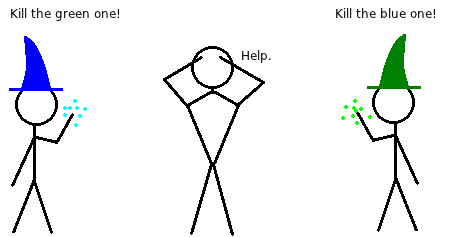
\includegraphics{Pics/Dominate.png}
\end{figure*}

You can control the actions of any humanoid creature through a telepathic link that you establish with the subject's mind.

If you and the subject have a common language, you can generally force the subject to perform as you desire, within the limits of its abilities. 
If no common language exists, you can communicate only basic commands, such as ``Come here,`` ``Go there,`` ``Fight,`` and ``Stand still.`` 
You know what the subject is experiencing, but you do not receive direct sensory input from it, nor can it communicate with you telepathically.

Once you have given a dominated creature a command, 
it continues to attempt to carry out that command to the exclusion of all other activities except those necessary for day-to-day survival 
(such as sleeping, eating, and so forth). 
Because of this limited range of activity, a Sense Motive check against DC 15 (rather than DC 25) 
can determine that the subject's behavior is being influenced by an enchantment effect (see the Sense Motive skill description).

Changing your instructions or giving a dominated creature a new command is the equivalent of redirecting a spell, so it is a move action.

By concentrating fully on the spell (a standard action), 
you can receive full sensory input as interpreted by the mind of the subject, though it still can't communicate with you. 
You can't actually see through the subject's eyes, so it's not as good as being there yourself, but you still get a good idea of what's going on.

Subjects resist this control, and any subject forced to take actions against its nature receives a new saving throw with a +2 bonus. 
Obviously self-destructive orders are not carried out. 
Once control is established, the range at which it can be exercised is unlimited, as long as you and the subject are on the same plane. 
You need not see the subject to control it.

If you don't spend at least 1 round concentrating on the spell each day, the subject receives a new saving throw to throw off the domination.

\nameref{Spell:AlignedProtection} or a similar spell can prevent you from exercising control or using the telepathic link while the subject is so warded, 
but such an effect neither prevents the establishment of domination nor dispels it.

\paragraph{Augment:} You can augment this spell in one or more of the following ways.
\begin{enumerate}
 \item If you spend 2 additional spell points, this spell can also affect an animal, fey, giant, magical beast, or monstrous humanoid.
 \item If you spend 4 additional spell points, this spell can also affect an aberration, 
 dragon, elemental, or outsider in addition to the creature types mentioned above.
 \item For every 2 additional spell points you spend, this spell can affect an additional target. 
 Any additional target cannot be more than 15 feet from another target of the spell.
 \item If you spend 1 additional spell point, this spell's duration changes to 1 hour.
 If you spend 2 additional spell points, this spell's duration changes to 1 day. 
 If you spend 4 additional spell points, this spell's duration changes to 1 day per caster level.
\end{enumerate}
\subsubsection{Dream}
\label{Spell:Dream}
Illusion (Phantasm) [Mind-Affecting]
\\ \textbf{Level:} Bard 5, Sor/Wiz 5
\\ \textbf{Components:} V, S
\\ \textbf{Casting Time:} 1 standard action
\\ \textbf{Range:} Unlimited
\\ \textbf{Target:} One creature
\\ \textbf{Duration:} Instantaneous; see text
\\ \textbf{Saving Throw:} Will negates; see text
\\ \textbf{Spell Resistance:} Yes
\\ \textbf{Spell Points:} 9

\emph{''Sleep tight. I'll be there.``}

You enter another creature's dream, either to deliver a message or to interrupt its sleep. These two functions of the spell work as follows:
\begin{list}{\labelitemi}{\leftmargin=1em}
 \item \emph{Deliver message:} You send a ghostly avatar of yourself into the subject's dream, allowing you to communicate as if you were standing face to face.
 This communication happens instantaneously, regardless of how long the conversation is - time is irrelevant when dreaming.
 The conversation lasts for as long as you both desire - if one participant wishes the conversation to end, it ends.
 When the participants wake up, they remember the conversation perfectly.
 You cannot use any spells, magic items, or any class or racial features during this dream conversation. 
 However, the skills Bluff, Diplomacy, Disguise, Intimidate, Knowledge, Sense Motive and Speak Language work perfectly.
 \item \emph{Nightmare:} You send a hideous and unsettling phantasmal vision to a specific creature that you name or otherwise specifically designate.
 The nightmare prevents restful sleep, leaving the subject fatigued and unable to regain arcane spells for the next 24 hours. 
 A successful will save negates this effect.
 The difficulty of the save depends on how well you know the subject and what sort of physical connection (if any) you have to that creature.
 See the table (\ref{tab:Scrying}) accompanying the scrying spell.
 Using this function adds the [Evil] descriptor to the spell.
 A creature under the influence of an \nameref{Spell:AlignedProtection} spell is immune to this aspect of the spell.
\end{list}
If the recipient is awake when you cast the spell, you can choose to cease casting (ending the spell) or to enter a trance until the recipient goes to sleep, 
whereupon you become alert again and complete the casting. If you are disturbed during the trance, 
you must succeed on a Concentration check as if you were in the midst of casting a spell or the spell ends. 
If you choose to enter a trance, you are not aware of your surroundings or the activities around you while in the trance.
You are defenseless, both physically and mentally, while in the trance. (You always fail any saving throw, for example.)

Creatures who don't sleep (such as elves, but not half-elves) or dream cannot be affected by this spell. 

\textbf{Augment:} If you spend 8 additional spell points, the Nightmare function of the spell becomes truly deadly.
If the subject fails the Will saving throw, it must also make a Fortitude save using the same DC or die of fright, never waking up again.
This adds the [Death] descriptor to the spell, in addition to the [Mind-Affecting] and [Evil] descriptor it already has.
\subsubsection{Dweomer Blockade}
\label{Spell:DweomerBlockade}
Abjuration
\\ \textbf{Level:} Blackguard 6
\\ \textbf{Components:} V, S
\\ \textbf{Casting Time:} 1 standard action
\\ \textbf{Range:} Medium (100 ft. + 10 ft./level)
\\ \textbf{Effect:} Ray
\\ \textbf{Duration:} 1 min./level
\\ \textbf{Saving Throw:} Will negates
\\ \textbf{Spell Resistance:} No
\\ \textbf{Spell Points:} 11

\emph{A nearly translucent ray springs from your outstretched hand.} 

You must make a ranged touch attack to hit the target. 
Any creature or object struck by the ray that fails a Will save is treated as being entirely within an \nameref{Spell:AntimagicField}, including the effect such a field has on a creature's magic items.
\subsubsection{Dweomer Rip}
\label{Spell:DweomerRip}
Abjuration
\\ \textbf{Level:} Magic 2
\\ \textbf{Components:} V, S
\\ \textbf{Casting Time:} 1 standard action
\\ \textbf{Range:} Close (25 ft. + 5 ft./2 levels)
\\ \textbf{Target:} One creature
\\ \textbf{Duration:} Instantaneous
\\ \textbf{Saving throw:} Fortitude half
\\ \textbf{Spell Resistance:} No
\\ \textbf{Spell Points:} 3

\emph{You pull at the strings of magic surrounding a creature, each cutting it like a thread.}

If a creature targeted by this spell has active spell effects on it at the time of casting,
it takes damage equal to twice the combined number of spell points that were spent on the spells, 
excluding those spell points spent to apply metamagic feats to the spells.
For example, a Wizard under the protection of a \nameref{Spell:MageArmor} spell augmented to cost 3 spell points and an unaugmented, quickened \nameref{Spell:Shield} spell
would take 8 points of damage.

A successful fortitude save halves the damage. The spells are not dispelled.
\paragraph{Augment:} For every 3 additional spell points you spend, this spell can affect an additional target.

\subsection{'E' Spells}
\subsubsection{Earthquake}
\label{Spell:Earthquake}
Evocation [Earth]
\\ \textbf{Level:} Destruction 7, Earth 7
\\ \textbf{Components:} V, S
\\ \textbf{Casting Time:} 1 standard action
\\ \textbf{Range:} Long (400 ft. + 40 ft./level)
\\ \textbf{Area:} 80-ft.-radius spread (S)
\\ \textbf{Duration:} 1 round
\\ \textbf{Saving Throw:} See text
\\ \textbf{Spell Resistance:} No
\\ \textbf{Spell Points:} 15

\emph{''Feel the ground tremble!``}

When you cast earthquake, an intense but highly localized tremor rips the ground. 
The shock knocks creatures down, collapses structures, opens cracks in the ground, and more. 
The effect lasts for 1 round, during which time creatures on the ground can't move or attack. 
A spellcaster on the ground must make a Concentration check (DC 20 + spell level) or lose any spell he or she tries to cast. 
The earthquake affects all terrain, vegetation, structures, and creatures in the area. 
The specific effect of an earthquake spell depends on the nature of the terrain where it is cast.

\begin{list}{\labelitemi}{\leftmargin=1em}
\item \emph{Cave, Cavern, or Tunnel:}
The spell collapses the roof, dealing 8d6 points of bludgeoning damage to any creature caught under the cave-in (Reflex half) and pinning that creature beneath the rubble (see below).
An earthquake cast on the roof of a very large cavern could also endanger those outside the actual area but below the falling debris.

\item \emph{Cliffs:}
Earthquake causes a cliff to crumble, creating a landslide that travels horizontally as far as it fell vertically. 
Any creature in the path takes 8d6 points of bludgeoning damage (Reflex half) and is pinned beneath the rubble (see below).

\item \emph{Open Ground:}
Each creature standing in the area must make a Reflex save or fall prone. 
Additionally, fissures (each 10d10' deep) open in the earth. And every creature on the ground has a 25\% chance of falling into one (a second reflex save prevents the fall). 
At the end of the spell, all fissures grind shut, killing any creatures still trapped within.

\item \emph{Structure:}
Any structure standing on open ground takes 100 points of damage, enough to collapse a typical wooden or masonry building, but not a structure built of stone or reinforced masonry. 
Hardness does not reduce this damage, nor is it halved as damage dealt to objects normally is. 
Any creature caught inside a collapsing structure takes 8d6 points of bludgeoning damage (Reflex half) and is pinned beneath the rubble (see below).

\item \emph{River, Lake, or Marsh:}
Fissures open underneath the water, draining away the water from that area and forming muddy ground. 
Soggy marsh or swampland becomes quicksand for the duration of the spell, sucking down creatures and structures. 
Each creature in the area must make a Reflex save or sink down in the mud and quicksand. 
At the end of the spell, the rest of the body of water rushes in to replace the drained water, possibly drowning those caught in the mud.
\end{list}
Any creature pinned beneath rubble is \emph{immobilized} and takes 1d6 points of nonlethal damage per minute while pinned. 
If a pinned character falls unconscious, he or she must make a DC 15 Constitution check or take 1d6 points of lethal damage each minute thereafter until freed or dead.
\subsubsection{Elemental Weapons}
\label{Spell:ElementalWeapons}
Evocation [see text]
\\ \textbf{Level:} Ranger 1
\\ \textbf{Components:} V
\\ \textbf{Casting Time:} 1 swift action
\\ \textbf{Range:} Personal
\\ \textbf{Target:} You
\\ \textbf{Duration:} 1 round
\\ \textbf{Spell Points:} 1

\emph{Your weapons hiss with the primal forces of nature.}

For the duration of this spell, all of your weapon attacks (including ranged attacks, but not your spells, spell-like abilities, or supernatural abilities) deal an additional 1d6 points of energy damage. Choose one of the following energy types upon casting: \emph{Cold}, \emph{Electricity}, or \emph{Fire}.
This spell's descriptor is the same as the type of energy you selected. 
The damage dealt by this spell stacks with any other elemental damage your weapon may deal.

\paragraph{Augment:} For two additional spell points you spend, this spell's damage increases by one die (d6).

\emph{Special:} Casting this spell does not provoke Attacks of Opportunity.
\subsubsection{Elfcloak}
\label{Spell:Elfcloak}
Divination
\\ \textbf{Level:} Ranger 1
\\ \textbf{Components:} V, S
\\ \textbf{Casting Time:} 1 standard action
\\ \textbf{Range:} Personal
\\ \textbf{Target:} You
\\ \textbf{Duration:} 10 min./level (D)
\\ \textbf{Spell Points:} 1

\emph{Your clothes and equipment subtly takes on the color and texture of nearby objects, including floors and walls.}

You gain a +5 competence bonus on Hide checks.

\paragraph{Augment:} For every additional spell point you spend, the Hide check bonus granted by this spell increases by 1.
\subsubsection{Endure Elements}
\label{Spell:EndureElements}
Abjuration
\\ \textbf{Level:} Blackguard 1, Paladin 1, Protection 1, Ranger 1, Sor/Wiz 1, Sun 1
\\ \textbf{Components:} V, S
\\ \textbf{Casting Time:} 1 standard action
\\ \textbf{Range:} Touch
\\ \textbf{Target:} Creature touched
\\ \textbf{Duration:} 24 hours
\\ \textbf{Saving Throw:} Will negates (harmless)
\\ \textbf{Spell Resistance:} Yes (harmless)
\\ \textbf{Spell Points:} 1

\emph{You fear no hail, drought, or storm.}

A creature protected by endure elements suffers no harm from being in a hot or cold environment. 
It can exist comfortably in conditions between -50 and 140 degrees Fahrenheit (between -45 and 60 degrees Celcius) without having to make Fortitude saves. 
The creature's equipment is likewise protected.

Endure elements doesn't provide any protection from fire or cold damage, 
nor does it protect against other environmental hazards such as smoke, lack of air, and so forth.

\paragraph{Augment:} You can augment this spell in one or more of the following ways.
\begin{enumerate}
\item If you spend two additional spell points, the subject of the spell does not treat slippery ice, areas of undergrowth, bogs or loose rubble as difficult terrain.
The subject does not have to pay extra movement in order to move through such terrain.
\item If you spend two additional spell points, the subject of the spell never risks catching on fire due to environmental fires.
\item If you spend two additional spell points, the subject of the spell is immune to the negative effects of environmental smoke and acid fume inhalation.
\end{enumerate}

\subsubsection{Energized Touch}
\label{Spell:ShockingGrasp}
Evocation [see text]%[Electricity]
\\ \textbf{Level:} Sor/Wiz 1
\\ \textbf{Components:} V, S
\\ \textbf{Casting Time:} 1 standard action
\\ \textbf{Range:} Touch
\\ \textbf{Target:} Creature or object touched
\\ \textbf{Duration:} Instantaneous
\\ \textbf{Saving Throw:} None
\\ \textbf{Spell Resistance:} Yes
\\ \textbf{Spell Points:} 1

\emph{*Zap!*}

\begin{figure*}
  \caption{Wizard incinerates unsuspecting victim at close range with \emph{Burning Hands}.}
  \centering
    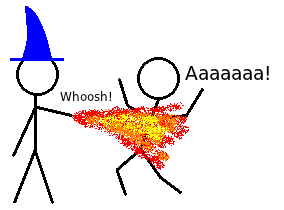
\includegraphics{Pics/BurningHands.png}
\end{figure*}

Your successful melee touch attack deals 1d8 points of energy damage. Choose one of the following energy types upon casting:
\begin{list}{\labelitemi}{\leftmargin=1em}
 \item Cold: A touch of this energy type deals +1 point of damage per die. This form of the spell is usually referred to as \emph{Chill Touch}.
 \item Electricity: When delivering a jolt of this energy type, you gain a +3 bonus on attack rolls if the opponent is wearing metal armor 
 (or made out of metal, carrying a lot of metal, or the like), 
 and a +2 bonus on caster level checks for the purpose of overcoming spell resistance.
 This form of the spell is usually referred to as \emph{Shocking Grasp}.
 \item Fire: A touch of this energy type deals +1 point of damage per die.
 This form of the spell is usually referred to as \emph{Burning Hands}.
 \item Sonic: A touch of this energy type deals -1 point of damage per die and ignores an object's hardness.
\end{list}

This spell's descriptor is the same as the type of energy you selected. 

\paragraph{Augment:} For every additional spell point you spend, this spell's damage increases by one die (d8).

\emph{Special:} Casting this spell does not provoke Attacks of Opportunity.


\subsubsection{Energy Arrow}
\label{Spell:EnergyArrow}
Evocation [see text]
\\ \textbf{Level:} Sor/Wiz 3
\\ \textbf{Components:} V, S
\\ \textbf{Casting Time:} 1 standard action
\\ \textbf{Range:} Close (25 ft. + 5 ft./2 levels)
\\ \textbf{Target:} Fifty projectiles, all of which must be in contact with each other at the time of casting
\\ \textbf{Duration:} 10 min./level
\\ \textbf{Saving Throw:} None
\\ \textbf{Spell Resistance:} No
\\ \textbf{Spell Points:} 5

\emph{You hand the ranger back his quiver, its contents glowing with magical energy.}

You turn ammunition (such as arrows, bolts, shuriken, or stones) into magical projectiles. 
Each piece of ammunition gains the benefit of one of the following enhancements:
\emph{Flaming}, \emph{Frost} or \emph{Shock}.
You choose the energy type at the time of casting.
Multiple castings of this spell do not stack, even if different enhancements are selected - 
if you cast the spell a second time on a projectile
before the spell's duration expires, the previous casting is overridden with respect to that projectile.
This allows the ammunition to bypass damage reduction as
if they were magic weapons, but they do not actually gain an enhancement bonus
(unless, of course, they are fired from a magical missile weapon).

This spell's descriptor matches the type of energy you imbue the projectiles with.

\paragraph{Augment:} If you spend 4 additional spell points, 
you can instead select from one of the following enhancements:
\emph{Flaming Burst}, \emph{Icy Burst}, and \emph{Shocking Burst}.

\subsubsection{Enervation}
\label{Spell:Enervation}
Necromancy
\\ \textbf{Level:} Necromancer 4
\\ \textbf{Components:} V, S
\\ \textbf{Casting Time:} 1 standard action
\\ \textbf{Range:} Close (25 ft. + 5 ft./2 levels)
\\ \textbf{Effect:} Ray of negative energy
\\ \textbf{Duration:} Instantaneous
\\ \textbf{Saving Throw:} None
\\ \textbf{Spell Resistance:} Yes
\\ \textbf{Spell Points:} 7

\emph{You point your finger and utter the incantation, releasing a black ray of crackling negative energy that suppresses the life force of any living creature it strikes.} 

You must make a ranged touch attack to hit.
If the attack succeeds, the subject gains 1d4 negative levels.

If the subject has at least as many negative levels as HD, it dies. 

Each negative level gives a creature a -1 penalty on attack rolls, saving throws, 
skill checks, ability checks, and effective level (for determining the power, duration, DC, and other details of spells or special abilities), 
and causes it to lose 5 hit points.
Spellcasters take additional penalties, as detailed under the \nameref{sec:NegativeLevels} section.

Assuming the subject survives, it regains lost levels after 1 hour. 
Usually, negative levels have a chance of permanently draining the victim's levels,
but the negative levels from enervation don't last long enough to do so.

An undead creature struck by the ray gains 1d4$\times$5 temporary hit points for 1 hour.

\paragraph{Augment:} For every 3 additional spell points you spend, this spell inflicts an additional negative level on a successful hit.
\subsubsection{Entangle}
\label{Spell:Entangle}
Transmutation
\\ \textbf{Level:} Plant 1, Ranger 1
\\ \textbf{Components:} V, S
\\ \textbf{Casting Time:} 1 standard action
\\ \textbf{Range:} Long (400 ft. + 40 ft./level)
\\ \textbf{Area:} Plants in a 20-ft.-radius spread
\\ \textbf{Duration:} 1 min./level (D)
\\ \textbf{Saving Throw:} Reflex partial; see text
\\ \textbf{Spell Resistance:} No
\\ \textbf{Spell Points:} 1

\emph{Grasses, weeds, bushes, and even trees wrap, twist, and entwine about everything in their path.} 

Creatures in the area or those that enter it are \emph{entangled}.
The creature can break free and move half its normal speed by using a full-round action to make a DC 20 Strength check or a DC 20 Escape Artist check. 
A creature that succeeds on a Reflex save is not entangled but can still move at only half speed through the area. 
Each round on your turn, the plants once again attempt to entangle all creatures that have avoided or escaped entanglement.

\paragraph{Augment:} If you spend 8 additional spell points, creatures in the area are \emph{immobilized} on a failed save rather than \emph{entangled}. The Strength or Escape Artist check DCs are not affected.

\subsubsection{Enthrall}
\label{Spell:Enthrall}
Enchantment (Charm) [Language Dependent, Mind-Affecting, Sonic]
\\ \textbf{Level:} Bard 2, Cleric 2
\\ \textbf{Components:} V, S
\\ \textbf{Casting Time:} 1 round
\\ \textbf{Range:} Medium (100 ft. + 10 ft./level)
\\ \textbf{Targets:} Any number of creatures
\\ \textbf{Duration:} 1 hour or less; see text
\\ \textbf{Saving Throw:} Will negates; see text
\\ \textbf{Spell Resistance:} Yes
\\ \textbf{Spell Points:} 3

\emph{''I have a dream. Ich bin ein Berliner! Now this is not the end, it is not even the beginning of the end!}

If you have the attention of a group of creatures, you can use this spell to hold them spellbound. To cast the spell, you must speak or sing without interruption for 1 full round. Thereafter, those affected give you their undivided attention, ignoring their surroundings. They are considered to have an attitude of friendly while under the effect of the spell.

A creature with more HD than your caster level remains aware of its surroundings and has an attitude of indifferent. It gains a new saving throw if it witnesses actions that it opposes.

The effect lasts as long as you speak or sing, to a maximum of 1 hour. Those enthralled by your words take no action while you speak or sing and for 1d3 rounds thereafter while they discuss the topic or performance. Those entering the area during the performance must also successfully save or become enthralled. The speech ends (but the 1d3-round delay still applies) if you lose concentration or do anything other than speak or sing.

If those not enthralled have unfriendly or hostile attitudes toward you, they can collectively make a Charisma check to try to end the spell by jeering and heckling. For this check, use the Charisma bonus of the creature with the highest Charisma in the group; others may make Charisma checks to assist. The heckling ends the spell if this check result beats your Charisma check result. Only one such challenge is allowed per use of the spell.

If any member of the audience is attacked or subjected to some other overtly hostile act, the spell ends and the previously enthralled members become immediately unfriendly toward you.

\emph{Note:} Clerics usually refer to this spell as \emph{Mass} rather than \emph{Enthrall}.
\subsubsection{Entropic Shield}
\label{Spell:EntropicShield}
Abjuration
\\ \textbf{Level:} Air 1, Luck 1
\\ \textbf{Components:} V, S
\\ \textbf{Casting Time:} 1 standard action
\\ \textbf{Range:} Personal
\\ \textbf{Target:} You
\\ \textbf{Duration:} 1 min./level (D)
\\ \textbf{Spell Points:} 1

\emph{A magical field appears around you, glowing with a chaotic blast of multicolored hues, deflecting incoming arrows, rays, and other ranged attacks.} 
 
Each ranged attack directed at you for which the attacker must make an attack roll (including a touch attack) has a 20\% miss chance.
This miss chance is not concealment. When a creature is under both concealment and Entropic Shield, use only the larger percentage miss chance.
Other attacks that simply work at a distance are not affected.

\paragraph{Augment:} For every additional spell point you spend, the miss chance offered by this spell increases by 5\%, to a maximum of 50\% for a 9-point additional expenditure.
\subsubsection{Ethereal Jaunt}
\label{Spell:EtherealJaunt}
Transmutation
\\ \textbf{Level:} Sor/Wiz 7
\\ \textbf{Components:} V, S
\\ \textbf{Casting Time:} 1 standard action
\\ \textbf{Range:} Touch
\\ \textbf{Target:} Creature touched
\\ \textbf{Duration:} 1 round/level (D)
\\ \textbf{Saving Throw:} Will negates
\\ \textbf{Spell Resistance:} Yes
\\ \textbf{Spell Points:} 13

\emph{The creature fades out of sight with the sound of someone exhaling softly.}

The subject becomes ethereal, along with your equipment. 
For the duration of the spell, the subject is in a place called the Ethereal Plane, which overlaps the normal, physical, Material Plane. 
When the spell expires, the subjects return to material existence.

An ethereal creature is invisible, insubstantial, and capable of moving in any direction, even up or down, albeit at half normal speed. 
An insubstantial creature can move through solid objects, including living creatures. 
An ethereal creature can see and hear on the Material Plane, but everything looks gray and ephemeral. 
Sight and hearing onto the Material Plane are limited to 60 feet.
Force effects and abjurations affect an ethereal creature normally. 
Their effects extend onto the Ethereal Plane from the Material Plane, but not vice versa. 
An ethereal creature can't attack material creatures, and spells you cast while ethereal affect only other ethereal things. 
Certain material creatures or objects have attacks or effects that work on the Ethereal Plane.
Treat other ethereal creatures and ethereal objects as if they were material.

If you end the spell while the subject is inside a material object (such as a solid wall), 
the subject is shunted off to the nearest open space and takes 1d6 points of damage per 5 feet that you so travel. 

\paragraph{Augment:} You can augment this spell in one or both of the following ways:
\begin{enumerate}
 \item For every two additional spell points you spend, this spell can affect an additional creature.
 \item If you spend two additional spell points, this spell's duration increases to 1 min./level.
\end{enumerate}
\subsubsection{Eyebite}
\label{Spell:Eyebite}
Necromancy [Evil]
\\ \textbf{Level:} Bard 6, Sor/Wiz 6
\\ \textbf{Components:} V, S
\\ \textbf{Casting Time:} 1 standard action
\\ \textbf{Range:} Close (25 ft. + 5 ft./2 levels)
\\ \textbf{Target:} One living creature
\\ \textbf{Duration:} Instantaneous; see text
\\ \textbf{Saving Throw:} Will negates
\\ \textbf{Spell Resistance:} Yes
\\ \textbf{Spell Points:} 11

\emph{''The evil eye is not a myth, as you will now learn to understand!``}

Each round, you may target a single living creature, striking it with waves of evil power.
Depending on the target's HD, this attack has as many as three effects. See the \nameref{tab:Eyebite} table for information on which effects apply.
The effects are concurrent.

\begin{tableonecolumn}
\caption{Eyebite}
\label{tab:Eyebite}
\begin{tabular}{|l|l|}
\hline
HD&Effect\\
\hline
10 or more&Sickened\\
9 or less&Panicked, sickened\\
4 or less&Comatose, panicked, sickened\\
\hline
\end{tabular}\\
\end{tableonecolumn}
The effects are:

\textbf{Sickened:} Sudden pain and fever sweeps over the subject's body, rendering it \emph{sickened}.
A creature affected by this spell remains sickened for 10 minutes per caster level. 
The effects cannot be negated by a remove disease or \nameref{Spell:Heal} spell, but a \nameref{Spell:RemoveCurse} is effective.

\textbf{Panicked:} The subject becomes \emph{panicked} for 1d4 rounds. 
Even after the panic ends, the creature remains shaken for 10 minutes per caster level, and 
it automatically becomes panicked again if it comes within sight of you during that time. 
This is a fear effect (it is possible to be immune to this part of the spell, while still being subject to the others normally).

\textbf{Comatose:} The subject falls into a catatonic coma for 10 minutes per caster level. 
During this time, it cannot be awakened by any means short of dispelling the effect or casting a \nameref{Spell:RemoveCurse} spell on it. 
This is not a sleep effect, and thus elves are not immune to it.

The spell lasts for 1 round per three caster levels. You must spend a move action each round after the first to target a foe. 

\paragraph{Augment:} You affect creatures more powerfully by spending additional spell points.
For each additional spell point you spend, a creature of 1 HD more is affected by the Panicked and Comatose effects of the spell.
For example, if you spend one additional spell point, a creature of 10 HD or less is Panicked and Sickened, and a creature of 5 HD or less is Comatose, Panicked, and Sickened.
\subsubsection{Expeditious Retreat}
\label{Spell:ExpeditiousRetreat}
Transmutation
\\ \textbf{Level:} Bard 1, Ranger 1, Sor/Wiz 1, Travel 1
\\ \textbf{Components:} V, S
\\ \textbf{Casting Time:} 1 standard action or 1 swift action; see text
\\ \textbf{Range:} Personal
\\ \textbf{Target:} You
\\ \textbf{Duration:} 1 min./level (D) or 1 round; see text
\\ \textbf{Spell Points:} 1

\emph{Each of your steps takes you a much farther distance than they by any rights should.}

All of the subject's modes of movement (including land movement, burrow, climb, fly, and swim) increase by 30 feet. This increase counts as an enhancement bonus, and it affects the subject's jumping distance as normal for increased speed. The spell does not grant new kinds of movement, it merely enhances those the subject already has.

At the time of casting, you make a choice. If you cast the spell as a standard action, the duration is 1 minute per level. 
If you cast it as a swift action, the duration is one round.

\paragraph{Augment:}  You can augment this spell in one or both of the following ways.
\begin{enumerate}
 \item For every 2 additional spell points you spend, the bonus to your speeds increases by 10'.
 \item If you spend 2 additional spell points, the spell's range changes to ''touch``, and the target changes to ''creature touched``. 
\end{enumerate}
\subsubsection{Explosive Runes}
\label{Spell:ExplosiveRunes}
Abjuration [Force]
\\ \textbf{Level:} Sor/Wiz 3
\\ \textbf{Components:} V, S
\\ \textbf{Casting Time:} 1 standard action
\\ \textbf{Range:} Touch
\\ \textbf{Target:} One touched object weighing no more than 10 lb.
\\ \textbf{Duration:} Permanent until discharged (D)
\\ \textbf{Saving Throw:} See text
\\ \textbf{Spell Resistance:} Yes

\emph{''Have a nice day, I have rigged this piece of paper to explode.``}

You trace these mystic runes upon a book, map, scroll, or similar object bearing written information. 
The runes detonate when read, dealing 5d6 points of force damage. 
Anyone next to the runes (close enough to read them) takes the full damage with no saving throw; 
any other creature within 10 feet of the runes is entitled to a Reflex save for half damage. 
The object on which the runes were written also takes full damage (no saving throw).
Any other objects within the 10 foot radius that carry another instance of the explosive runes
are burned out, the explosive runes disappating harmlessly.

You and any characters you specifically instruct can read the protected writing without triggering the runes. 
Likewise, you can remove the runes whenever desired. 
Another creature can remove them with a successful \nameref{Spell:DispelMagic} spell %or erase spell, 
but attempting to dispel the runes and failing to do so triggers the explosion.
Since you automatically succeed on all dispel checks against spells you cast yourself, 
you cannot trigger your own explosive runes with \nameref{Spell:DispelMagic}.

Note: Magic traps such as explosive runes are hard to detect and disable. 
A rogue (only) can use the Search skill to find the runes and Disable Device to thwart them. 
The DC in each case is 25 + spell level, or 28 for explosive runes.

\paragraph{Augment:} For every additional spell point you spend, this spell's damage increases by 1d6.
%In addition, for every two spell points you spend to improve the spell's damage, its saving throw DC increases by 1.
\subsection{'F' Spells}
\subsubsection{Faerie Fire}
\label{Spell:FaerieFire}
Evocation [Light]
\\ \textbf{Level:} Fire 1
\\ \textbf{Components:} V, S
\\ \textbf{Casting Time:} 1 standard action
\\ \textbf{Range:} Long (400 ft. + 40 ft./level)
\\ \textbf{Area:} Creatures and objects within a 5-ft.-radius burst
\\ \textbf{Duration:} 1 min./level (D)
\\ \textbf{Saving Throw:} None
\\ \textbf{Spell Resistance:} Yes
\\ \textbf{Spell Points:} 1

\emph{A pale glow surrounds the subjects.} 

All creatures within the burst are outlined, and shed light as candles. 
Outlined creatures do not benefit from the concealment normally provided by darkness (though a magical darkness effect functions normally if more spell points were spent on the darkness effect than on the Faerie Fire spell), \nameref{Spell:Blur}, \emph{invisibility}, or similar effects. 
The light is too dim to have any special effect on undead or dark-dwelling creatures vulnerable to light. 
The faerie fire can be blue, green, or violet, according to your choice at the time of casting. 
The faerie fire does not cause any harm to the objects or creatures thus outlined.

\paragraph{Augment:} For every additional spell point you spend, you can create an additional 5' radius burst of Faerie Fire to erupt somewhere within range. The bursts need not be adjacent to one another.
\subsubsection{False Life}
\label{Spell:FalseLife}
Necromancy
\\ \textbf{Level:} Assassin 3, Blackguard 2, Sor/Wiz 2
\\ \textbf{Components:} V, S
\\ \textbf{Casting Time:} 1 standard action
\\ \textbf{Range:} Personal
\\ \textbf{Target:} You
\\ \textbf{Duration:} 1 hour/level or until depleted; see text
\\ \textbf{Spell Points:} Assassin 5, Blackguard 3, Sor/Wiz 3

\emph{You harness the power of unlife to grant yourself a limited ability to avoid death.} 

While this spell is in effect, you gain 1d10 temporary hit points.

\paragraph{Augment:} Every 2 additional spell points spent increase the temporary hit points you gain by 1d10.

\subsubsection{False Vision}
\label{Spell:FalseVision}
Illusion (Glamer)
\\ \textbf{Level:} Bard 5, Sor/Wiz 5, Trickery 5
\\ \textbf{Components:} V, S
\\ \textbf{Casting Time:} 1 standard action
\\ \textbf{Range:} Touch
\\ \textbf{Area:} 40-ft.-radius emanation
\\ \textbf{Duration:} 1 hour/level (D)
\\ \textbf{Saving Throw:} None
\\ \textbf{Spell Resistance:} No
\\ \textbf{Spell Points:} 9

\emph{''If they are looking, they will be in for a surprise.``}

Any divination (scrying) spell used to view anything within the area of this spell instead receives a false image, as defined by you at the time of casting. 
The false image the scryer sees functions as if generated by an \nameref{Spell:Image} spell, augmented with as many points as were spent on casting the
False Vision spell.
As long as the duration lasts, you can concentrate to change the image as desired. 
While you aren't concentrating, the image remains static.
\subsubsection{Feeblemind}
\label{Spell:Feeblemind}
Enchantment (Compulsion) [Mind-Affecting]
\\ \textbf{Level:} Sor/Wiz 5
\\ \textbf{Components:} V, S
\\ \textbf{Casting Time:} 1 standard action
\\ \textbf{Range:} Medium (100 ft. + 10 ft./level)
\\ \textbf{Target:} One creature
\\ \textbf{Duration:} Instantaneous
\\ \textbf{Saving Throw:} Will negates; see text
\\ \textbf{Spell Resistance:} Yes
\\ \textbf{Spell Points:} 9

\emph{''Not so smart now, Mr. Wizard?``}

If the target creature fails a Will saving throw, its Intelligence and Charisma scores each drop to 1. 
The affected creature is unable to use Intelligence- or Charisma-based skills, cast spells, understand language, or communicate coherently. 
Still, it knows who its friends are and can follow them and even protect them. 
The subject remains in this state until a \nameref{Spell:Heal}, \nameref{Spell:LimitedWish} , 
\nameref{Spell:Miracle}, or \nameref{Spell:Wish} spell is used to cancel the effect of the feeblemind. 
A creature that can cast arcane spells, such as a sorcerer or a wizard, takes a -4 penalty on its saving throw.

\subsubsection{Fear}
\label{Spell:Fear}
Necromancy [Fear, Mind-Affecting]
\\ \textbf{Level:} Bard 1, Blackguard 1, Death 1, Evil 1, Necromancer 1
\\ \textbf{Components:} V, S
\\ \textbf{Casting Time:} 1 standard action
\\ \textbf{Range:} Close (25 ft. + 5 ft./2 levels)
\\ \textbf{Target:} One living creature with 5 or fewer HD
\\ \textbf{Duration:} 1d4 rounds or 1 round; see text
\\ \textbf{Saving Throw:} Will partial
\\ \textbf{Spell Resistance:} Yes
\\ \textbf{Spell Points:} 1

\emph{You raise your hand and intone words of dread.}

The affected creature becomes \emph{frightened}. 
If the subject succeeds on a Will save, it is instead \emph{shaken} for 1 round. 
Creatures with 6 or more Hit Dice cannot be \emph{frightened} by this spell, only becoming \emph{shaken} even on a failed save.

\paragraph{Augment:} You can augment this spell in one or more of the following ways.
\begin{enumerate}
\item If you spend two additional spell points, the range of the spell increases to Medium.
\item For every two additional spell points spent, the spell can affect an additional creature.
\item If you spend two additional spell points, instead of becoming \emph{frightened} on a failed save, the subject becomes \emph{panicked}.
\end{enumerate}
In addition, for every additional spell point spent on augmenting the spell, the spell can \emph{frighten} a creature with one more HD.
\subsubsection{Fiendish Flight}
\label{Spell:FiendishFlight}
Transmutation [Evil]
\\ \textbf{Level:} Blackguard 3

\emph{The subject grows large batlike wings.}

This spell functions as the \nameref{Spell:Fly} spell (including its augmentation option), except as noted here, and that the flight is due to physical wings the subject grows (which matters for effects like those caused by tanglefoot bags).
\subsubsection{Fireball}
\label{Spell:Fireball}
Evocation [see text]
\\ \textbf{Level:} Evoker 2
\\ \textbf{Components:} V, S
\\ \textbf{Casting Time:} 1 standard action
\\ \textbf{Range:} Long (400 ft. + 40 ft./level)
\\ \textbf{Area:} 20-ft.-radius burst
\\ \textbf{Duration:} Instantaneous
\\ \textbf{Saving Throw:} Reflex half or Fortitude half; see text
\\ \textbf{Spell Resistance:} Yes
\\ \textbf{Spell Points:} 3

\emph{If the application of Fireball did not solve your problem, you failed to apply it in sufficient amounts.}

A fireball spell is an explosion of energy that detonates with a low roar and deals 3d6 points of damage to every creature within the area. 
Unattended objects also take this damage. 

You choose between cold, electricity, fire, or sonic damage at the time of casting.
If the damage caused to an interposing barrier shatters or breaks through it, the fireball may continue beyond the barrier if the area permits; 
otherwise it stops at the barrier just as any other spell effect does. 

You point your finger and determine the range (distance and height) at which the fireball is to burst. 
A glowing, pea-sized bead streaks from the pointing digit and, unless it impacts upon a material body or solid barrier prior to attaining the prescribed range, 
blossoms into the fireball at that point. (An early impact results in an early detonation.)

The name of the spell refers to the fire version of the spell, which was the form of the spell originally discovered.
Although other forms of the spell were later unearthed, ''Fireball'' remains as its name.
\begin{list}{\labelitemi}{\leftmargin=1em}
 \item Cold: A burst of this energy type deals +1 point of damage per die. 
 The saving throw to reduce damage from a cold burst is a Fortitude save instead of a Reflex save.
 \item Electricity: A burst of this energy type provides a +2 bonus to the save DC
 and a +2 bonus on caster level checks for the purpose of overcoming spell resistance.
 \item Fire: A burst of this energy type deals +1 point of damage per die.
 \item Sonic: A burst of this energy type deals -1 point of damage per die and ignores an object's hardness.
\end{list}
The spell has all side effects you would normally expect a flash of energy to produce - fire causes small, flammable objects to catch fire, cold causes exposed bodies of water to get a thin coating of ice, and so on.
The explosion also creates significant pressure, which has effects of its own. 
Light, unattended objects are hurled away from the blast radius, and glass windows may break.

This spell's descriptor is the same as the type of energy you selected. 

\paragraph{Augment:} For every additional spell point you spend, this spell's damage increases by one die (d6).

\emph{Special:} Fireballs are extraordinarily hard to dodge. The base saving throw DC against a Fireball spell is 
10 + the number of spell points spent on the spell and its augments + your key ability modifier, 
rather than as described in the section on \nameref{sec:SavingThrow}s.
\subsubsection{Fire Seeds}
\label{Spell:FireSeeds}
Conjuration (Creation) [Fire]
\\ \textbf{Level:} Fire 6, Sun 6
\\ \textbf{Components:} V, S
\\ \textbf{Casting Time:} 1 standard action
\\ \textbf{Range:} Touch
\\ \textbf{Targets:} Up to four touched acorns or up to eight touched holly berries
\\ \textbf{Duration:} 10 min./level or until used
\\ \textbf{Saving Throw:} None or Reflex half; see text
\\ \textbf{Spell Resistance:} No
\\ \textbf{Spell Points:} 11

\emph{You channel fire into the seeds until they are about to burst.}

Depending on the version of fire seeds you choose, you turn acorns into splash weapons that you or another character can throw, or you turn holly berries into bombs that you can detonate on command. Each version has separate augmentation options.

\begin{list}{\labelitemi}{\leftmargin=1em}
 \item \emph{Acorn Grenades:} As many as four acorns turn into special splash weapons that can be hurled as far as 100 feet. A ranged touch attack roll is required to strike the intended target. Together, the acorns are capable of dealing 13d6 points of fire damage, divided up among the acorns as you wish (in increments of one die of damage).

Each acorn explodes upon striking any hard surface. In addition to its regular fire damage, it deals 1 point of splash damage per die, and it ignites any combustible materials within 10 feet. A creature within this area that makes a successful Reflex saving throw takes only half damage; a creature struck directly is not allowed a saving throw.
\paragraph{Augment:} For every additional spell point you spend on the \emph{Acorn Grenades} version of the spell, the combined damage dealt by the grenades increases by one die (d6).
 \item \emph{Holly Berry Bombs:} You turn as many as eight holly berries into special bombs. 
The holly berries are usually placed by hand, since they are too light to make effective thrown weapons (they can be tossed only 5 feet). If dropped from a height, use the rules for aiming splash weapons at a square. If you are within 200 feet and speak a word of command (a standard action), each berry instantly bursts into flame, causing 1d8+11 points of fire damage to every creature in a 5-foot radius burst and igniting any combustible materials within 5 feet. A creature in the area that makes a successful Reflex saving throw takes only half damage.
\paragraph{Augment:} For every additional spell point you spend on the \emph{Holly Berry Bombs} version of the spell, each bomb deals an additional point of fire damage.
\end{list}
\subsubsection{Fire Storm}
\label{Spell:FireStorm}
Evocation [Fire]
\\ \textbf{Level:} Fire 7
\\ \textbf{Components:} V, S
\\ \textbf{Casting Time:} 1 standard action
\\ \textbf{Range:} Medium (100 ft. + 10 ft./level)
\\ \textbf{Area:} Two 10-ft. cubes per level (S)
\\ \textbf{Duration:} Instantaneous
\\ \textbf{Saving Throw:} Reflex half
\\ \textbf{Spell Resistance:} Yes
\\ \textbf{Spell Points:} 13

\emph{The whole area is shot through with sheets of roaring flame.} 

Creatures within the area take 13d6 points of fire damage.
However, the spell does not harm natural vegetation, ground cover, and any plant creatures in the area that you specifically exclude from damage.

\paragraph{Augment:} For every additional spell point you spend, this spell's damage increases by one die (d6).
\subsubsection{Finger of Death}
\label{Spell:FingerOfDeath}
Necromancy [Death]
\\ \textbf{Level:} Death 7, Sor/Wiz 7
\\ \textbf{Components:} V, S
\\ \textbf{Casting Time:} 1 standard action
\\ \textbf{Range:} Close (25 ft. + 5 ft./2 levels)
\\ \textbf{Target:} One living creature
\\ \textbf{Duration:} Instantaneous
\\ \textbf{Saving Throw:} Fortitude partial
\\ \textbf{Spell Resistance:} Yes
\\ \textbf{Spell Points:} 13

\emph{``AVADA KEDAVRA!''}

You can slay any one living creature within range. 
The target is entitled to a Fortitude saving throw to survive the attack. 
If the save is successful, the creature instead takes 3d6 points of damage +1 point per caster level.

The subject might die from damage even if it succeeds on its saving throw. 

\paragraph{Augment:} For every 3 additional spell points you spend, this spell can target an additional creature within range.
\subsubsection{Fist of the Deity}
\label{Spell:FistOfTheDeity}
Evocation [see text]
\\ \textbf{Level:} Chaos 4, Evil 4, Good 4, Law 4
\\ \textbf{Components:} V, S
\\ \textbf{Casting Time:} 1 standard action
\\ \textbf{Range:} Medium (100 ft. + 10 ft./level)
\\ \textbf{Area:} 20-ft.-radius burst
\\ \textbf{Duration:} Instantaneous; see text
\\ \textbf{Saving Throw:} Will partial; see text
\\ \textbf{Spell Resistance:} Yes
\\ \textbf{Spell Points:} 7

\emph{You blast the area with energy, but only the unworthy must fear.}

When casting this spell, select an alignment. The spell gains a descriptor matching that alignment.

Any creature within the spell's area not of the selected aligment takes 4d8 points of damage, 
unless it is an outsider with an alignment subtype of the alignment opposed to the alignment you selected,
in which case it takes 7d6 points of damage.
In addition, all creatures not of the selected alignment suffer an additional penalty, depending on the alignment you selected:
\begin{list}{\labelitemi}{\leftmargin=1em}
 \item \emph{Chaos:} The chaotic version of this spell is referred to as \emph{Chaos Hammer}, and stuns creatures for 1d2 rounds.
 \item \emph{Evil:} The evil version of this spell is referred to as \emph{Unholy Blight}, and blinds creatures for 2d4 rounds.
 \item \emph{Good:} The good version of this spell is referred to as \emph{Holy Smite}, and nauseates creatures for 1d4 rounds.
 \item \emph{Law:} The lawful version of this spell is referred to as \emph{Order's Wrath}, and dazes creatures for 1d2 rounds.
\end{list}
A successful will saving throw reduces the damage by half and negates the additional penalty.

\paragraph{Augment:} For every 2 additional spell points you spend, 
the damage against outsiders of an opposed alignment increases by 2d6, 
and the damage against other creatures increases by 1d8.
\subsubsection{Flame Blade}
\label{Spell:FlameBlade}
Conjuration (Creation) [Fire]
\\ \textbf{Level:} Fire 2
\\ \textbf{Components:} V, S
\\ \textbf{Casting Time:} 1 standard action
\\ \textbf{Range:} 0 ft.
\\ \textbf{Effect:} A weapon made of fire
\\ \textbf{Duration:} 1 min./level
\\ \textbf{Saving Throw:} None
\\ \textbf{Spell Resistance:} No
\\ \textbf{Spell Points:} 3

\emph{You cause a blazing beam of red-hot fire to spring from your hand and solidify.}

You conjure a weapon made of pure, solidified fire.
This can be any kind of melee weapon with which you are proficient.

The weapon functions as a normal, physical weapon of its kind, except that all damage it deals is converted to fire damage\footnote{If you have access to the Fire domain, some of the damage may be again converted to divine damage.}.

No one but you can use this weapon. If someone successfully disarms you of the weapon, it immediately disappears in a burst of flame that deals 1d6 points of fire damage to the one that disarmed you of it.
The weapon then reforms in your hands at the start of your next turn.
The weapon cannot be sundered or otherwise damaged (though it can be dispelled).

The weapon can be improved by spells and other effects that affect normal weapons, such as the \nameref{Spell:MagicWeapon} spell (but not by actual magical enhancements, since the weapon doesn't last long enough to have those placed on it). 

\paragraph{Augment:} For every 3 additional spell points you spend, the weapon deals 1d6 points of fire damage in addition to its normal (converted) damage.
\subsubsection{Flame Strike}
\label{Spell:FlameStrike}
Evocation [Fire]
\\ \textbf{Level:} Fire 4, Sun 4, War 4
\\ \textbf{Components:} V, S
\\ \textbf{Casting Time:} 1 standard action
\\ \textbf{Range:} Medium (100 ft. + 10 ft./level)
\\ \textbf{Area:} Cylinder (10-ft. radius, 40 ft. high)
\\ \textbf{Duration:} Instantaneous
\\ \textbf{Saving Throw:} Reflex partial; see text
\\ \textbf{Spell Resistance:} Yes
\\ \textbf{Spell Points:} 9

\emph{A vertical column of divine fire roars downward.}

The spell deals 7d6 points of fire damage, and knocks every creature within the area prone.
A successful reflex save reduces the damage by half, and prevents the creature from being knocked down.

\paragraph{Augment:} For every additional spell point you spend on this spell, its damage is increased by one die (d6).
\subsubsection{Flaming Sphere}
\label{Spell:FlamingSphere}
Evocation [Fire]
\\ \textbf{Level:} Fire 2, Sor/Wiz 2
\\ \textbf{Components:} V, S
\\ \textbf{Casting Time:} 1 standard action
\\ \textbf{Range:} Medium (100 ft. + 10 ft./level)
\\ \textbf{Effect:} 5-ft.-diameter sphere
\\ \textbf{Duration:} 1 round/level
\\ \textbf{Saving Throw:} None
\\ \textbf{Spell Resistance:} Yes
\\ \textbf{Spell Points:} 3

\emph{A burning globe of fire rolls in whichever direction you point and burns those it strikes.} 

The sphere you create appears anywhere within range, and moves 30 feet per round. As part of this movement, it can ascend or jump up to 30 feet to strike a target. 
If it enters (or is created in) a space with a creature, it stops moving for the round and deals 2d6 points of fire damage to that creature.
A flaming sphere rolls over barriers less than 4 feet tall. 
It ignites flammable substances it touches and illuminates the same area as a torch would.

The sphere moves as long as you actively direct it (a move action for you); 
otherwise, it merely stays at rest and burns. It can be extinguished by any means that would put out a normal fire of its size. 
The surface of the sphere has a spongy, yielding consistency and so does not cause damage except by its flame. 
It cannot push aside unwilling creatures or batter down large obstacles. 
A flaming sphere winks out if it exceeds the spell's range.

\paragraph{Augment:} You can augment this spell in one or both of the following ways:
\begin{enumerate}
 \item If you spend 2 additional spell points, you can direct the spell as a free action rather than as a move action.
 \item For every 2 additional spell points you spend, this spell's damage increases by one die (d6).
\end{enumerate}
\subsubsection{Floating Disk}
\label{Spell:FloatingDisk}
Evocation [Force]
\\ \textbf{Level:} Sor/Wiz 1
\\ \textbf{Components:} V, S
\\ \textbf{Casting Time:} 1 standard action
\\ \textbf{Range:} Close (25 ft. + 5 ft./2 levels)
\\ \textbf{Effect:} 3-ft.-diameter disk of force
\\ \textbf{Duration:} 1 hour/level
\\ \textbf{Saving Throw:} None
\\ \textbf{Spell Resistance:} No
\\ \textbf{Spell Points:} 1

\emph{``A horse would have been too passé.''}

You create a slightly concave, circular plane of force that follows you about and carries loads for you. 
The disk is 3 feet in diameter and 1 inch deep at its center. 
It can hold 100 pounds of weight per caster level. (If used to transport a liquid, its capacity is 2 gallons.) 
The disk floats approximately 3 feet above the ground at all times and remains level. 
You can mentally command it to move around horizontally within spell range. 
It can move up to twice your normal speed each round (In other words, it can keep up if you perform a single or double move, but not if you run).
If not otherwise directed, it maintains a constant interval of 5 feet between itself and you. 
The disk winks out of existence when the spell duration expires. 
The disk also winks out if you or the disk attempt to move beyond range or if you try to take the disk more than 3 feet away from the surface beneath it. 
When the disk winks out, whatever it was supporting falls to the surface beneath it.

\paragraph{Augment:} If you spend an additional 6 spell points, you can command the disk to move vertically as well as horizontally, and the limit of
the disk not being able to move more than 3 feet from the ground no longer applies.

\subsubsection{Fly}
\label{Spell:Fly}
Transmutation
\\ \textbf{Level:} Transmuter 3, Travel 3
\\ \textbf{Components:} V, S
\\ \textbf{Casting Time:} 1 standard action
\\ \textbf{Range:} Touch
\\ \textbf{Target:} Creature touched
\\ \textbf{Duration:} 1 min./level
\\ \textbf{Saving Throw:} Will negates (harmless)
\\ \textbf{Spell Resistance:} Yes (harmless)
\\ \textbf{Spell Points:} 5

\emph{There is no surer sign of an individual being powerful than the one of defying the pull of the earth.}

\begin{figure*}
  \caption{Sorcerer and Fighter discuss the merits of the \emph{Fly} spell.}
  \centering
    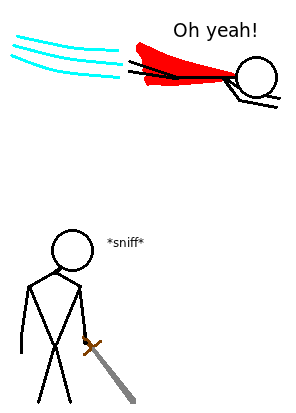
\includegraphics{Pics/Fly.png}
\end{figure*}

The subject can fly at a speed of 40 feet (or 30 feet if it wears medium or heavy armor, or if it carries a medium or heavy load). 
It can ascend at half speed and descend at double speed, and its maneuverability is good. 
Using a fly spell requires only as much concentration as walking, so the subject can attack or cast spells normally. 
The subject of a fly spell can charge but not run, and it cannot carry aloft more weight than its maximum load, plus any armor it wears.

Should the spell duration expire while the subject is still aloft, the magic fails slowly. 
The subject floats downward 60 feet per round for 1d6 rounds. 
If it reaches the ground in that amount of time, it lands safely. 
If not, it falls the rest of the distance, taking 1d6 points of damage per 10 feet of fall. 

If the spell is dispelled or negated by an \nameref{Spell:AntimagicField}, 
the subject falls like a rock, taking the appropriate falling damage.

\paragraph{Augment:} If you spend 4 additional spell points, the spell's duration increases to 1 hour per level.

When using this spell for long-distance movement, you can hustle without taking nonlethal damage 
(a forced march still requires Constitution checks). 
This means you can cover 64 miles (103 kilometres) in an eight-hour period of flight (or 48 miles (77 kilometres) at a speed of 30 feet).

\subsubsection{Fog}
\label{Spell:Fog}
Conjuration (Creation)
\\ \textbf{Level:} Air 1, Assassin 1, Conjurer, Water 1
\\ \textbf{Components:} V, S
\\ \textbf{Casting Time:} 1 standard action
\\ \textbf{Range:} 20 ft.
\\ \textbf{Effect:} Fog spreads in 20-ft. radius, 20 ft. high, centered on you
\\ \textbf{Duration:} 1 min./level
\\ \textbf{Saving Throw:} None
\\ \textbf{Spell Resistance:} No
\\ \textbf{Spell Points:} 1

\emph{A misty vapor arises around you. }

You create a bank of fog, which is stationary once created. 
The fog obscures all sight, including darkvision, beyond 5 feet. 
A creature 5 feet away has concealment (attacks have a 20\% miss chance). 
Creatures farther away have total concealment (50\% miss chance, and the attacker cannot use sight to locate the target).

A moderate wind (11+ mph), such as from a \nameref{Spell:GustOfWind} spell, disperses the fog in 4 rounds. 
A strong wind (21+ mph) disperses the fog in 1 round. 

This spell does not function underwater.

\paragraph{Augment:} You can augment the spell in one or more of the following ways:
\begin{enumerate}
 \item If you spend 2 additional spell points, the spell's duration is 10 minutes per level rather than 1 minute per level.
 \item If you spend 2 additional spell points, the spell's range increases to Medium (allowing you to create banks of fog not centered on you).
 \item If you spend 6 additional spell points, the fog becomes so thick as to be nearly solid. Anyone attempting to move through a solid fog cloud
has his speed reduced to 5 feet (assuming the speed was more than 5 feet to begin with), and takes a -2 penalty on all melee attack rolls with weapons other
than piercing weapons. The solid vapors prevent effective ranged weapon attacks (except for magic rays and the like). A creature or object that falls into
solid fog is slowed, so that each 10 feet of vapor that it passes through reduces falling damage by 1d6.
A creature can't take a 5-foot step while in solid fog.
\end{enumerate}
\subsubsection{Food and Water}
\label{Spell:FoodAndWater}
Transmutation
\\ \textbf{Level:} Water 1
\\ \textbf{Components:} V, S
\\ \textbf{Casting Time:} 1 standard action
\\ \textbf{Range:} Close (25 ft. + 5 ft./2 levels)
\\ \textbf{Target:} 1 cu. ft./level of contaminated food and water
\\ \textbf{Duration:} Instantaneous
\\ \textbf{Saving Throw:} Will negates (object)
\\ \textbf{Spell Resistance:} Yes (object)
\\ \textbf{Spell Points:} 1

\emph{Raising your hand towards the granary, you remove from the food all signs of taint.}

This spell makes spoiled, rotten, poisonous, or otherwise contaminated food and water pure and suitable for eating and drinking. 
This spell does not prevent subsequent natural decay or spoilage. 
Aligned water and similar food and drink of significance is spoiled by this spell, but the spell has no effect on creatures of any type nor upon magic potions.

\emph{Note:} Water weighs about 8 pounds per gallon. One cubic foot of water contains roughly 8 gallons and weighs about 60 pounds.

\paragraph{Augment:} If you spend 4 additional spell points, the transmutation becomes fundamentally more powerful. Instead of targeting contaminated food and water, it targets nonliving, nonmagical, unattended objects weighing up to 1 lb./level. This transforms the objects into an equivalent weight of food. Each pound of food so created is sufficient to nourish one creature for 24 hours (similar to a pound of trail rations). 
The food so created is simple - highly nourishing, if rather bland.
The food decays and becomes inedible after 24 hours, although it can be kept fresh for another 24 hours by casting another (unaugmented) instance of the spell on it.

\subsubsection{Forbiddance}
\label{Spell:Forbiddance}
Abjuration
\\ \textbf{Level:} Planes 6
\\ \textbf{Components:} V, S
\\ \textbf{Casting Time:} 6 rounds
\\ \textbf{Range:} Medium (100 ft. + 10 ft./level)
\\ \textbf{Area:} Eleven 60-ft. cubes (S)
\\ \textbf{Duration:} Permanent
\\ \textbf{Saving Throw:} See text
\\ \textbf{Spell Resistance:} Yes
\\ \textbf{Spell Points:} 11

\emph{``You are not welcome in this place!''}

Forbiddance seals an area against all planar travel into or within it. 
This includes all teleportation spells (such as \nameref{Spell:DimensionDoor} and \nameref{Spell:Teleport}), plane shifting, astral travel, ethereal travel, and all summoning spells. 
Such effects simply fail automatically.

In addition, when casting the spell, you select between one and eight alignments that the Forbiddance further wards against. You cannot select your own alignment.
Creatures of those alignments must succeed on a Will save immediately after entering a square covered by the Forbiddance or be \emph{Blown Away} in the same direction from which the creature entered.
Creatures who succeed on the saving throw can enter the area of the Forbiddance, but still experience a powerful and painful feeling of aversion.
A creature of one of the selected alignments who starts its turn in the area of the Forbiddance must make a Fortitude save or take 6d6 points of damage. This save is repeated each round for as long as the creature remains in the area\footnote{Dragging helpless creatures into a Forbiddance area that wards against it is usually considered too cruel a tactic for most Good orgnanizations to support it, unless dealing with extraordinarily Evil creatures, such as undead or Evil outsiders.}.
% In addition, it damages entering creatures whose alignments are different from yours. 
% The effect on those attempting to enter the warded area is based on their alignment relative to yours (see below). 
% A creature inside the area when the spell is cast takes no damage unless it exits the area and attempts to reenter, at which time it is affected as normal.
% 
% \begin{list}{\labelitemi}{\leftmargin=1em}
% \item \emph{Alignments identical}
% No effect. The creature may enter the area freely (although not by planar travel).
% \item \emph{Alignments different with respect to either law/chaos or good/evil}
% The creature takes 6d6 points of damage. A successful Will save halves the damage, and spell resistance applies.
% \item \emph{Alignments different with respect to both law/chaos and good/evil}
% The creature takes 12d6 points of damage. A successful Will save halves the damage, and spell resistance applies.
% \end{list}

At your option, the abjuration can include a password, in which case creatures of the selected alignments can avoid the negative effects by speaking the password as they enter the area. 
You must select this option (and the password) at the time of casting.

\nameref{Spell:DispelMagic} cannot dispel a forbiddance effect unless the dispeller's level is at least as high as your caster level.

You can't have multiple overlapping forbiddance effects. 
In such a case, the more recent effect stops at the boundary of the older effect.

\emph{Experience Cost:} 300XP. If a password is desired, this requires an additional 200XP.

\paragraph{Augment:} For every additional spell point you spend, you can place Forbiddance upon an additional 60' cube.
\subsubsection{Forced Visions}
\label{Spell:ForcedVisions}
Divination [Mind-Affecting]
\\ \textbf{Level:} Sor/Wiz 3
\\ \textbf{Components:} V, S
\\ \textbf{Casting Time:} 1 standard action
\\ \textbf{Range:} Medium (100 ft. + 10 ft./ level)
\\ \textbf{Target:} One creature with an intelligence score of 3 or more
\\ \textbf{Duration:} 1 round/level
\\ \textbf{Saving Throw:} Will negates; see text
\\ \textbf{Spell Resistance:} Yes
\\ \textbf{Spell Points:} 5

\emph{Your victim staggers around, unable to tell the images in its head from what is happening around it.}

Unlike most divination spells, this spell is less about retrieving information than it is to force it upon someone.
For the duration of this spell, the subject's mind is haunted by fairly useless (but factually accurate) 
visions of his past, present, and sometimes even future.
Unless he succeeds on a Will save, the subject is \emph{stunned} for the first round of the spell's duration, the images
momentarily overwhelming its conscious mind. Every round thereafter, at the start of his turn, he must succeed on a will save or be \emph{confused} for that round. 
When such a save succeeds, the subject can suppress the images to the point where it no
longer interferes with his actions, effectively ending the spell.

If desired, the GM can use the following table to determine the kind of vision the subject suffers:
\begin{center}
\small
\begin{tabular}{|p{1cm}|p{5.4cm}|}
\hline
d\% & Vision\\
result&\\
\hline
1-30 & Childhood memories\\
31-60 & Memories regarding the subject's love life\\
61-70 & Memory resulting in the character shouting out an embarrassing fact about himself\\
71-80 & Memories regarding the character's line of work or training\\
81-90 & A vision of the character as an old man (Does not have to imply that he \emph{will} be old, only that it's a possibility.)\\
91-95 & A vision of the character's surroundings, distorted and confusing\\
96-99 & A vision of the character, as seen from the caster's eyes\\
100 & A truly useful vision of the future\\
\hline
\end{tabular}
\end{center}
\paragraph{Augment:} For every 2 additional spell points you spend, the subject is stunned for one additional round of the
spell's duration, rather than just the first. A successful will save in a subsequent round still ends the spell.

\subsubsection{Foresight}
\label{Spell:Foresight}
Divination
\\ \textbf{Level:} Diviner 9, Knowledge 9
\\ \textbf{Components:} V, S
\\ \textbf{Casting Time:} 1 standard action
\\ \textbf{Range:} Personal or touch
\\ \textbf{Target:} See text
\\ \textbf{Duration:} 10 min./level
\\ \textbf{Saving Throw:} None or Will negates (harmless)
\\ \textbf{Spell Resistance:} No or Yes (harmless)
\\ \textbf{Spell Points:} 17

\emph{Suddenly, everything seems exceedingly predictable.}

This spell grants you a powerful sixth sense in relation to yourself or another. 
Once foresight is cast, you receive instantaneous warnings of impending danger or harm to the subject of the spell. 
You are never surprised or flat-footed. 
In addition, the spell gives you a general idea of what action you might take to best protect yourself,
and thus gives you a +2 insight bonus to AC and Reflex saves. 
This insight bonus is lost whenever you would lose a Dexterity bonus to AC.

When another creature is the subject of the spell, you receive warnings about that creature. 
You must communicate what you learn to the other creature for the warning to be useful, 
and the creature can be caught unprepared in the absence of such a warning. 
Shouting a warning, yanking a person back, and even telepathically communicating (via an appropriate spell) 
can all be accomplished before some danger befalls the subject, provided you act on the warning without delay. 
The subject, however, does not gain the insight bonus to AC and Reflex saves.

\subsubsection{Form of the Avian}
\label{Spell:FormAvian}
Transmutation (Polymorph)
\\ \textbf{Level:} Animal 3, Ranger 3, Transmuter 3
\\ \textbf{Components:} V,S
\\ \textbf{Casting Time:} 1 standard action
\\ \textbf{Range:} Touch
\\ \textbf{Target:} Willing living creature touched
\\ \textbf{Duration:} 10 min./level (D)
\\ \textbf{Saving Throw:} None
\\ \textbf{Spell Resistance:} No
\\ \textbf{Spell Points:} 5

\emph{The subject assumes the form of a winged bird, like that of an eagle or a swan.}

The subject undergoes the following changes:
\\ Its size changes to small.
\\ Its base strength score changes to 10.
\\ Its base dexterity score changes to 16.
\\ It gains a bite attack that deals 1d4 points of damage + your strength modifier.
This bite can be used as either a primary natural attack or a secondary natural attack.
\\ It gains the benefit of the Weapon Finesse feat.
\\ The avian form has physical wings and can fly at a speed of 60', with good maneuverability. 
\\ Its land speed changes to 10'.

However, the form has no hands, preventing the subject from using weapons and items requiring fine manipulation (although it can use its feet to hold things that can be easily gripped). It cannot provide somatic components.

\paragraph{Augment:} You can Augment this spell in one or more of the following ways:
\begin{enumerate}
 \item For every additional spell point you spend, the subject's fly speed increases by 10'.
 \item If you spend 4 additional spell points, the subject's size becomes medium when casting the spell,
 its strength score changes to 18 and its dexterity score changes to 14.
 Its bite and talon attacks (if any) have their base damage dice increased by one step.
 \item If you spend 2 additional spell points, the subject gains two talon attacks in addition to the bite
 attack. These can only be used as secondary natural attacks. The talons deal 1d3 points of
 damage + $1/2$ the subject's strength modifier. 
\end{enumerate}

\subsubsection{Form of the Dragon}
\label{Spell:FormDragon}
Transmutation (Polymorph)
\\ \textbf{Level:} Transmuter 6
\\ \textbf{Components:} V,S
\\ \textbf{Casting Time:} 1 standard action
\\ \textbf{Range:} Touch
\\ \textbf{Target:} Willing living creature touched
\\ \textbf{Duration:} 1 round/level (D)
\\ \textbf{Saving Throw:} None
\\ \textbf{Spell Resistance:} No
\\ \textbf{Spell Points:} 11

\emph{The subject assumes the form of a majestic metallic or chromatic dragon.}

The subject undergoes the following changes:
\\ Its size changes to large (long).
\\ Its base strength score changes to 26.
\\ Its base natural armor changes to 7.
\\ It gains a bite attack that deals 1d8 points of damage + its strength modifier, which is a primary natural attack.
\\ It gains two claw attacks that deal 1d6 + its strength modifier, which are secondary natural attacks.
\\ It gains two wing attacks that deal 1d4 + 1/2 its strength modifier, which are secondary natural attacks.
\\ Its land speed changes to 30'.
\\ The draconic form has physical wings and can fly at a speed of 100', with poor maneuverability.

The form is that of a quadruped, granting the subject a +4 bonus on ability checks made to resist being bull rushed or tripped when standing on the ground.
The form's front claws are capable of fine manipulation, enabling the subject to use items and provide somatic components as if it had hands.
However, the subject is not able to simultaneously walk and hold items in both front claws.

\paragraph{Augment:} You can Augment this spell in one or more of the following ways:
\begin{enumerate}
 \item For every additional spell point you spend, the strength score of the assumed form increases by 1.
 \item If you spend 4 additional spell points, the subject's size becomes huge when casting the spell, and
 its strength score changes to 28.
 The subject's bite, claw, wing and tail (if the subject has any) attacks have their base damage dice increased by one step.
 \item If you spend 4 additional spell points, the subject gains a tail attack that deals 1d8 points of damage + 
 $1 1/2$ times its strength modifier, which is a secondary natural attack.
\end{enumerate}

\subsubsection{Form of the Elemental}
\label{Spell:FormElemental}
Transmutation (Polymorph)
\\ \textbf{Level:} Air 7, Earth 7, Fire 7, Transmuter 7, Water 7.
\\ \textbf{Components:} V,S
\\ \textbf{Casting Time:} 1 standard action
\\ \textbf{Range:} Touch
\\ \textbf{Target:} Willing living creature touched
\\ \textbf{Duration:} 1 min./level (D)
\\ \textbf{Saving Throw:} None
\\ \textbf{Spell Resistance:} No
\\ \textbf{Spell Points:} 13

\emph{The subject's hair constantly moves as in a slight breeze of air.}

The subject's inner structure is radically altered, being now formed of pure elemental power. Its shape is not significantly affected.

At the time of casting, select an element. The subject gains bonuses according to the selected element.
\begin{list}{\labelitemi}{\leftmargin=1em}
 \item \emph{Air Elemental:} The subject gains a fly speed of 60' (perfect maneuverability) for the duration of the spell.
 \item \emph{Earth Elemental:} The subject gains the Earth Glide ability, like a real Earth Elemental.
 \item \emph{Fire Elemental:} The subject gains immunity to fire, and vulnerability to cold.
 Those it hits with melee attacks must make a DC 15 reflex save or catch fire.
 The subject illuminates its surroundings like a torch, although it is not glaringly obvious that the subject is the source of the light.
 \item \emph{Water Elemental:} The subject gains immunity to cold, and vulnerability to fire.
 It can breathe water as well as it can breathe air, and gains a swim speed equal to its base land speed.
\end{list}
In addition to the qualities that depend on the selected energy type, the subject gains darkvision out to 60 feet, immunity to poison, sleep effects, paralysis, stunning, critical hits, and flanking.

% \paragraph{Augment:} If you spend 4 additional spell points, the creature is able to retain more of itself throughout the transformation.
% The creature retains all its class features when polymorphed (notably, allowing spellcasting).
% This is an exception to the general rules of Polymorph subschool spells.
\subsubsection{Form of the Fiend}
\label{Spell:FormFiend}
Transmutation (Polymorph) [Evil]
\\ \textbf{Level:} Blackguard 6, Planes 6
\\ \textbf{Components:} V,S
\\ \textbf{Casting Time:} 1 standard action
\\ \textbf{Range:} Personal
\\ \textbf{Target:} You
\\ \textbf{Duration:} 10 min./level (D)
\\ \textbf{Spell Points:} 11

\emph{You assume the form of a fiendish creature, your eyes turning black, and batlike wings sprouting from your back.}

You undergo the following changes:
\\ You grow physical wings and can fly at a speed of 100', with good maneuverability. 
\\ You gain darkvision out to 60', and low-light vision. This special darkvision allows you to see through even Magical darkness.
\\ You gain immunity to electricity and fire.
\\ You gain resistance to acid 10 and cold 10.
\\ You gain immunity to poison.
\\ You gain the telepathy special ability, out to 100 feet.
\\ Once during the spell's duration, you may use \nameref{Spell:SummonDemon} or \nameref{Spell:SummonDevil} as a spell-like ability. Caster level 9th. The casting time is as normal for the spell in question.

Your form is humanoid, with functioning hands and legs.

\paragraph{Augment:} For every additional spell point you spend, the caster level of the summoning ability increases by 1.

\subsubsection{Form of the Fish}
\label{Spell:FormFish}
Transmutation (Polymorph)
\\ \textbf{Level:} Animal 3, Ranger 3, Transmuter 3
\\ \textbf{Components:} V,S
\\ \textbf{Casting Time:} 1 standard action
\\ \textbf{Range:} Touch
\\ \textbf{Target:} Willing living creature touched
\\ \textbf{Duration:} 10 min./level (D)
\\ \textbf{Saving Throw:} None
\\ \textbf{Spell Resistance:} No
\\ \textbf{Spell Points:} 5

\emph{The subject assumes the form of a water-dwelling creature, such as a tuna or seal.}

The subject undergoes the following changes:
\\ Its size changes to small.
\\ Its base strength score changes to 14.
\\ It gains a bite attack that deals 1d6 points of damage + 1 1/2 times its strength modifier, which the subject's primary natural attack.
\\ The subject loses its land speed, and gains a swim speed of 40'.

At your option at the time of casting, the subject may gain the ability to breathe water, but lose the ability to breathe air for the duration of the spell.

Your aquatic form has no limbs that can be used to manipulate items or provide somatic components, but you may be able to hold some items (or even creatures) in your mouth, depending on your size.

\paragraph{Augment:} You can Augment this spell in one or both of the following ways:
\begin{enumerate}
 \item For every 2 additional spell points you spend, the swim speed of the form increases by 10'.
 \item For every 3 additional spell points you spend, the strength score of the form increases by 4, and it is one size category larger (to a maximum of colossal, for a 15-point additional expenditure).
 This increases the damage die of the bite attack by one step.
\end{enumerate}
\subsubsection{Form of the Horror}
\label{Spell:FormHorror}
Transmutation (Polymorph)
\\ \textbf{Level:} Blackguard 5, Transmuter 5
\\ \textbf{Components:} V,S
\\ \textbf{Casting Time:} 1 standard action
\\ \textbf{Range:} Touch
\\ \textbf{Target:} Willing living creature touched
\\ \textbf{Duration:} 1 round./level (D)
\\ \textbf{Saving Throw:} None
\\ \textbf{Spell Resistance:} No
\\ \textbf{Spell Points:} 9

\emph{The subject assumes the form of a horrific aberration, sprouting tentacles in place of arms and its skin turning into a slimy hide.}

The subject undergoes the following changes:
\\ Its base strength score changes to 18.
\\ Its base natural armor changes to 5.
\\ It gains two tentacle attacks that deal 1d8 + its strength modifier, which are primary natural attacks.
It gains the benefit of the improved grab special attack when making these tentacle attacks.
The reach of these tentacles is the same as that of a creature one size category larger than the subject's actual size.

The form functions as if one size larger than its actual size with regards to grappling (granting the appropriate size bonus on grapple checks, and allowing it to grab larger creatures).

The form has no hands, preventing the subject from using weapons and items requiring fine manipulation. It cannot provide somatic components.
However, the tentacles can be used to hold items.

\paragraph{Augment:} You can Augment this spell in one or both of the following ways:
\begin{enumerate}
 \item For every two additional spell points you spend, the subject gains an additional tentacle and tentacle attack.
 \item For every four additional spell points you spend, the effective size of the subject's form with respect to reach and grappling increases one additional category above its own.
\end{enumerate}
\subsubsection{Form of the Iron Golem}
\label{Spell:FormIronGolem}
Transmutation (Polymorph)
\\ \textbf{Level:} Earth 8, Transmuter 8
\\ \textbf{Components:} V,S
\\ \textbf{Casting Time:} 1 standard action
\\ \textbf{Range:} Touch
\\ \textbf{Target:} Willing living creature touched
\\ \textbf{Duration:} 1 minute./level (D)
\\ \textbf{Saving Throw:} None
\\ \textbf{Spell Resistance:} No
\\ \textbf{Spell Points:} 15

\emph{This spell transforms the subject's body into living iron.}

The subject undergoes the following changes:
\\ It gains damage reduction 15/adamantine. 
\\ It gains immunity to blindness, critical hits, ability score damage, deafness, disease, drowning, electricity, poison, stunning, and all spells or attacks that affect its physiology or respiration, because it has no physiology or respiration while this spell is in effect.
\\ It becomes vulnerable to the Rusting Grasp spell and rust monsters. 
\\ Its size changes to large (tall).
\\ Its base strength score changes to 30.
\\ Its base dexterity score changes to 6.
\\ Its base natural armor changes to 8.
\\ It gains a slam attack that deals 1d10 + 1 1/2 times its strength modifier, which is a primary natural attack.
\\ The subject's land speed changes to 20'.

The subject cannot drink (and thus can't use potions) or play wind instruments. 
Its weight increases by a factor of ten, causing it to sink in water like a stone (the subject loses any swim speed it may have, and it automatically fails all swim checks).
However, it could survive the crushing pressure and lack of air at the bottom of the ocean - at least until the spell duration expires.

\paragraph{Augment:} You can Augment this spell in one or more of the following ways:
\begin{enumerate}
 \item For every additional spell point you spend, the strength score of the assumed form increases by 2.
 \item For every additional spell point you spend, the damage reduction offered by this spell increases by 2.
\end{enumerate}
\subsubsection{Form of the Plant}
\label{Spell:FormPlant}
Transmutation (Polymorph)
\\ \textbf{Level:} Plant 2
\\ \textbf{Components:} V,S
\\ \textbf{Casting Time:} 1 standard action
\\ \textbf{Range:} Personal
\\ \textbf{Target:} You
\\ \textbf{Duration:} 1 hour/level (D)
\\ \textbf{Spell Points:} 3

\emph{You assume the form of a tree, bush, a vine or other kind of appropriately sized plant.}

You undergo the following changes:
\\ Your size changes to large (tall), large (long), or medium, chosen at the time of casting.
\\ You lose your strength and dexterity scores (they change to ``-``), becoming immobile.
\\ You gain immunity to poison, sleep effects, paralysis, stunning, and critical hits.
\\ You lose your ability to see and hear, but you gain the Blindsense ability out to 60'.

You become rooted when on the ground, granting you a +20 bonus on ability checks made to resist being bull rushed or tripped when standing on the ground. Your climb DC is 10.
Use the maximum carrying capacity of your unpolymorphed form to determine whether the the plant can support the climber's weight.

You gain a +16 racial bonus on hide checks when in forested areas, and a +30 bonus on Disguise checks made to pretend being a tree.

\paragraph{Augment:} You can Augment this spell in one of the following ways:
\begin{enumerate}
 \item If you spend 2 additional spell points, you can choose to become a small or tiny plant.
 \item If you spend 6 additional spell points, you can choose to become a diminutive or fine plant.
 \item If you spend 4 additional spell points, you can choose to become a huge plant.
 \item If you spend 6 additional spell points, you can choose to become a gargantuan plant.
 \item If you spend 8 additional spell points, you can choose to become a colossal plant.
\end{enumerate}
\subsubsection{Form of the Predator}
\label{Spell:FormCarnivore}
Transmutation (Polymorph)
\\ \textbf{Level:} Animal 4, Ranger 4, Transmuter 4
\\ \textbf{Components:} V,S
\\ \textbf{Casting Time:} 1 standard action
\\ \textbf{Range:} Touch
\\ \textbf{Target:} Willing living creature touched
\\ \textbf{Duration:} 1 round/level (D)
\\ \textbf{Saving Throw:} None
\\ \textbf{Spell Resistance:} No
\\ \textbf{Spell Points:} 7

\emph{The subject assumes the form of a large, dangerous beast, like a tiger or a bear.}

The subject undergoes the following changes:
\\ Its size changes to large (long).
\\ Its base strength score changes to 22.
\\ Its base natural armor changes to 5.
\\ It gains two claw attacks that deal 1d8 + its strength modifier, which are primary natural attacks.
\\ It gains a bite attack that deals 2d6 points of damage + $1/2$ its strength modifier, which is a secondary natural attack.
\\ Its land speed changes to 40'.

Its form is that of a quadruped, granting it a +4 bonus on ability checks made to resist being bull
rushed or tripped when standing on the ground. 
However, the form has no hands, preventing the subject from using weapons and items requiring fine manipulation (although it can use its feet to hold things that can be easily gripped). It cannot provide somatic components.

\paragraph{Augment:} You can Augment this spell in one or more of the following ways:
\begin{enumerate}
 \item For every two additional spell points you spend, the strength score of the assumed form increases by 3.
 \item If you spend 6 additional spell points, the subject's size becomes huge when casting the spell, and its strength score changes to 28.
 The bite and claw attacks have their base damage dice increased by one step.
 \item If you spend 12 additional spell points, the subjects' size becomes gargantuan when casting the spell, and its strength score changes to 34.
 The bite and claw attacks have their base damage dice increased by two steps.
 \item For every two additional spell points you spend, the base natural armor of the assumed form increases by 1.
\end{enumerate}
\subsubsection{Form of the Scout}
\label{Spell:FormScout}
Transmutation (Polymorph)
\\ \textbf{Level:} Transmuter 2
\\ \textbf{Components:} V,S
\\ \textbf{Casting Time:} 1 standard action
\\ \textbf{Range:} Touch
\\ \textbf{Target:} Willing living creature touched
\\ \textbf{Duration:} 10 min./level (D)
\\ \textbf{Saving Throw:} None
\\ \textbf{Spell Resistance:} No
\\ \textbf{Spell Points:} 3

\emph{The subject assumes the form of a fast, agile creature.}

The subject undergoes the following changes:
\\ Its size changes to tiny.
\\ Its base strength score changes to 2.
\\ Its base dexterity score changes to 14.
\\ Its land speed changes to 30'.
\\ It gains no natural attacks.

The form is that of a quadruped, granting the subject a +4 bonus on ability checks made to resist being bull rushed or tripped when standing on the ground.
The form has no hands, preventing the subject from using weapons and items requiring fine manipulation. It cannot provide somatic components.
It may be able to use its mouth to hold items, within the limits of its new strength score.

As a tiny creature, the subject has a +8 size bonus on hide checks. It also gains a complimentary +8 racial bonus on move silently checks.

At the time of casting, you choose one enhanced mode of movement from the following list, which the subject gains:
\begin{list}{\labelitemi}{\leftmargin=1em}
 \item A burrow speed of 20'.
 \item A climb speed of 20'.
 \item A swim speed of 20'.
 \item An increase in base land speed, up to 50'.
\end{list}

\paragraph{Augment:} You can Augment this spell in one or two of the following ways:
\begin{enumerate}
 \item For every 2 additional spell points you spend, the burrow, climb, swim, or land speed increases by 10'.
 The mode of movement so augmented is the same as the one you chose to enhance at the time of casting.
 \item If you spend 4 additional spell points, the subject's size decreases to diminutive, its base strength score changes to 1, and its base dexterity score changes to 16. The racial bonus on move silently checks increases to +12, and as a diminutive creature, the subject has a +12 size bonus on hide checks.
 \item If you spend 12 additional spell points, the subject's size decreases to fine, its base strength score changes to 1, and its base dexterity score changes to 20. The racial bonus on move silently checks increases to +16, and as a fine creature, the subject has a +16 size bonus on hide checks.
\end{enumerate}
\subsubsection{Form of the Titan}
\label{Spell:FormTitan}
Transmutation (Polymorph)
\\ \textbf{Level:} Strength 9
\\ \textbf{Components:} V,S
\\ \textbf{Casting Time:} 1 standard action
\\ \textbf{Range:} Touch
\\ \textbf{Target:} Willing living creature touched
\\ \textbf{Duration:} 1 round/level (D)
\\ \textbf{Saving Throw:} None
\\ \textbf{Spell Resistance:} No
\\ \textbf{Spell Points:} 17

\emph{The subject assumes the form of an enormous giant with bulging muscles.}

The subject undergoes the following changes:
\\ Its size changes to Huge.
\\ Its base strength score changes to 43.
\\ Its base natural armor changes to 19.
\\ It gains two slam attacks that deal 1d8 + its strength modifier, which are secondary natural attacks.
\\ It can use \nameref{Spell:ChainLightning} as a spell-like ability. Its save DC is charisma-based, and its caster level is equal to the subject's hit die.
\\ Its land speed changes to 60'.

Any weapon the subject may wield is magically resized to huge, and bypasses damage reduction as if it were made of adamantine.
The subject's body shape is mostly unchanged.

\paragraph{Augment:} For every additional spell point you spend, the subject's strength score increases by 2, and its natural armor increases by 1.
\subsubsection{Form of the Treant}
\label{Spell:FormTreant}
Transmutation (Polymorph)
\\ \textbf{Level:} Plant 5, Ranger 5, Transmuter 5
\\ \textbf{Components:} V,S
\\ \textbf{Casting Time:} 1 standard action
\\ \textbf{Range:} Touch
\\ \textbf{Target:} Willing living creature touched
\\ \textbf{Duration:} 1 round/level (D)
\\ \textbf{Saving Throw:} None
\\ \textbf{Spell Resistance:} No
\\ \textbf{Spell Points:} 9

\emph{The subject assumes the form of a mobile plant creature.}

The subject undergoes the following changes:
\\ Its size changes to large (tall).
\\ Its base strength score changes to 22.
\\ Its base natural armor changes to 9, and it gains damage reduction 10/slashing.
\\ It gains a slam attack that deals 1d8 points of damage + $1 1/2$ times its strength modifier, which is a primary natural attack.
\\ It gains the trample special attack, which follows the normal rules for such attacks.
\\ It gains immunity to poison, sleep effects, paralysis, stunning, and critical hits.
\\ Its land speed changes to 20'.

The form is partially rooted when on the ground, granting the subject a +10 bonus on ability checks made to resist being bull
rushed or tripped when standing on the ground.

The form has no hands, preventing the subject from using weapons and items requiring fine manipulation. It cannot provide somatic components.
However, the subject can bend its appendages to pick up objects.

The subject gains a +16 racial bonus on hide checks when in forested areas, and a +16 bonus on Disguise checks made to pretend being a tree.

\paragraph{Augment:} You can Augment this spell in one or more of the following ways:
\begin{enumerate}
 \item For every additional spell point you spend, the natural armor of the assumed form increases by 1.
 \item If you spend 4 additional spell points, the subject's size becomes huge when casting the spell, and its strength score changes to 26.
 The slam attack has its base damage die increased by one step.
 \item If you spend 8 additional spell points, the subject's size becomes gargantuan when casting the spell, and its strength score changes to 30.
 The slam attack has its base damage die increased by two steps.
\end{enumerate}
\subsubsection{Form of the Vermin}
\label{Spell:FormVermin}
Transmutation (Polymorph)
\\ \textbf{Level:} Transmuter 4, Vermin 4
\\ \textbf{Components:} V,S
\\ \textbf{Casting Time:} 1 standard action
\\ \textbf{Range:} Touch
\\ \textbf{Target:} Willing living creature touched
\\ \textbf{Duration:} 1 min./level (D)
\\ \textbf{Saving Throw:} None; see text
\\ \textbf{Spell Resistance:} No
\\ \textbf{Spell Points:} 7

\emph{The subject assumes the form of a gigantic insect, arachnid, crustacean or other generally repugnant creature.}

The subject undergoes the following changes:
\\ Its size changes to medium.
\\ Its base strength score changes to 18.
\\ It gains a sting attack that deals 2d6 points of damage + $1 1/2$ times its strength modifier, which is a primary natural attack.
The stinger is poisonous, dealing 1d6 points of primary and secondary dexterity damage. The poison's save DC is equal to this spell's save DC.
If the spell ends, all poison the subject has secreted immediately disappears, including poison that has been injected into a creature but has yet to deal its secondary damage. 
However, any damage the poison may already have inflicted remains.
Using this poison against a sapient creature (intelligence score of 3 or above) is an evil act.
\\Its land speed changes to 40'.

The form has multiple pairs of legs, granting the subject a +4 bonus on ability checks made to resist being bull rushed or tripped when standing on the ground. 
It gains a climb, swim or burrow speed of 20', chosen at the time of casting.

The form has no hands, preventing the subject from using weapons and items requiring fine manipulation. It cannot provide somatic components.

\paragraph{Augment:} You can Augment this spell in one or more of the following ways:
\begin{enumerate}
 \item If you spend 2 additional spell points, the subject's size becomes large (long) when casting the spell, and its strength score changes to 20.
 The sting attack (and claw or slam attacks, if you have them) has its base damage die increased by one step.
 \item If you spend 6 additional spell points, the subject's size becomes huge when casting the spell, and its strength score changes to 24.
 The sting attack (and claw or slam attacks, if you have them) has its base damage die increased by two steps. 
 The poison's primary and secondary dexterity damage increases to 1d8.
 \item If you spend 2 additional spell points, the subject gains two slam or claw attacks (your choice).
 These secondary attacks deal 1d6 points of damage + $1/2$ the subject's strength modifier.
 \item For every additional spell point you spend, the stinger's poison save DC increases by 1 above and beyond that normally offered by a spell of this power.
\end{enumerate}
\subsubsection{Form of the Viper}
\label{Spell:FormViper}
Transmutation (Polymorph)
\\ \textbf{Level:} Transmuter 4, Vermin 4
\\ \textbf{Components:} V,S
\\ \textbf{Casting Time:} 1 standard action
\\ \textbf{Range:} Touch
\\ \textbf{Target:} Willing living creature touched
\\ \textbf{Duration:} 1 min./level (D)
\\ \textbf{Saving Throw:} None; see text
\\ \textbf{Spell Resistance:} No
\\ \textbf{Spell Points:} 7

\emph{The subject assumes the form of a dangerous snake.}

The subject undergoes the following changes:
\\ Its size changes to large (long).
\\ Its base strength score changes to 20.
\\ It gains a bite attack that deals 1d8 points of damage + $1 1/2$ times its strength modifier, which is a primary natural attack.
The bite is poisonous, dealing 1d6 points of primary and secondary constitution damage. The poison's save DC is equal to this spell's save DC.
If the spell ends, all poison the subject has secreted immediately disappears, including poison that has been injected into a creature, but has yet to deal its secondary damage. However, any damage the poison may already have inflicted remains.
Using this poison against a sapient creature (intelligence score of 3 or above) is an evil act.
\\ The subject gains the constrict special attack. It deals damage equal to the damage dealt by the bite attack, except the constriction damage is bludgeoning damage, and does not deliver poison.
The subject does not provoke an attack of opportunity when starting a grapple as if it had the Improved Grapple feat.
\\ Its land speed changes to 20'.

The form has no legs, granting the subject immunity to trip attacks, and a +4 bonus on ability checks made to resist being bull rushed when standing on the ground.

The viper form has no limbs that can be used to manipulate items, but the subject may be able to hold some items in its mouth, depending on the form's size.
\paragraph{Augment:} You can Augment this spell in one or more of the following ways:
\begin{enumerate}
 \item If you spend 6 additional spell points, the subject's size becomes huge when casting the spell, and its strength score changes to 24.
 The bite attack has its base damage die increased by one step.
 \item If you spend 12 additional spell points, the subject's size becomes gargantuan when casting the spell, and its strength score changes to 30.
 The bite attack has its base damage die increased by two steps.
 \item For every additional spell point you spend, the bite's poison save DC increases by 1 above and beyond that
 normally offered by a spell of this power.
\end{enumerate}

\subsubsection{Fortune of the Gods}
\label{Spell:FortuneOfTheGods}
Evocation
\\ \textbf{Level:} Luck 9
\\ \textbf{Components:} V, S
\\ \textbf{Casting Time:} 1 standard action
\\ \textbf{Range:} Personal
\\ \textbf{Target:} You
\\ \textbf{Duration:} 1 round/level
\\ \textbf{Spell Points:} 17

\emph{Your divine patron smiles upon you, subtly twisting all circumstances slightly in your favor.}

For the duration of the spell, whenever you make a d20 roll, roll two dice and choose the result you prefer. Any ability that allows you to reroll a die only affects one of the dice you roll.
\subsubsection{Free Run}
\label{Spell:FreeRun}
Transmutation
\\ \textbf{Level:} Ranger 6, Travel 7
\\ \textbf{Components:} V, S
\\ \textbf{Casting Time:} 1 standard action
\\ \textbf{Range:} Personal and touch
\\ \textbf{Target:} You and up to 5 touched willing creatures
\\ \textbf{Duration:} 1 hour/level
\\ \textbf{Saving Throw:} None
\\ \textbf{Spell Resistance:} No
\\ \textbf{Spell Points:} Ranger 11, Travel 13

\emph{''A distant drumbeat sounds in your ears, and you feel an irresistible urge to run.``}

For the duration of this spell, the overland distance traveled by the subjects is multiplied by 10 for any given time period.
This multiplication applies only if traveling by foot, not when mounted or using another form of assisted transportation (such as a ship).

Further, the subjects' overland movement is not hindered by negative terrain conditions (as long as the terrain is actually passable), traveling as easily over difficult terrain as a well-made highway.
For example, the subjects could travel across a trackless jungle at full (tenfold) speed, rather than $1/4$ speed.

This does not affect the subjects' tactical movement speed.

\paragraph{Augment:} For every 2 additional spell points you spend, this spell can affect an additional target.

\subsubsection{Free Step}
\label{Spell:FreeStep}
Conjuration (Teleportation)
\\ \textbf{Level:} Planes 1, Travel 1
\\ \textbf{Components:} V
\\ \textbf{Casting Time:} 1 swift action
\\ \textbf{Range:} 10 feet
\\ \textbf{Target:} You
\\ \textbf{Duration:} Instantaneous
\\ \textbf{Spell Points:} 1

\emph{A quick step through the astral plane is useful for getting around.}

You instantly teleport yourself to an unoccupied space within the spell's range.
You must have line of sight and line of effect to the destination.

\paragraph{Augment:} For every additional spell point you spend, the spell's range increases by 5 feet.

\subsubsection{Freedom}
\label{Spell:Freedom}
Abjuration
\\ \textbf{Level:} Sor/Wiz 9
\\ \textbf{Components:} V, S
\\ \textbf{Casting Time:} 1 standard action
\\ \textbf{Range:} Close (25 ft. + 5 ft./2 levels) or see text
\\ \textbf{Target:} One creature
\\ \textbf{Duration:} Instantaneous, then 1 round/level; see text
\\ \textbf{Saving Throw:} Will negates (harmless)
\\ \textbf{Spell Resistance:} Yes
\\ \textbf{Spell Points:} 17

\emph{Freedom is not a spell. It is an idea.}

The subject is freed from the effect of a \nameref{Spell:Binding}, \nameref{Spell:Imprisonment}, \nameref{Spell:Maze} and/or a \nameref{Spell:TemporalStasis} spell.

To free a creature from imprisonment or \nameref{Spell:Maze}, 
you must know its name and background, and you must cast this spell at the spot where it was entombed or banished into the maze.

The freedom effect itself is instantaneous. 
But in addition, the subject of the Freedom spell gains the benefits of the \nameref{Spell:FreedomOfMovement} after the Freedom spell has been cast,
except for that the duration of the Freedom of Movement is 1 round per level.
It is possible to cast the Freedom spell on a creature that isn't imprisoned simply to give it this secondary benefit.

\paragraph{Augment:} For every 2 additional spell points you spend, this spell can target an additional creature within range.
\subsubsection{Freedom of Movement}
\label{Spell:FreedomOfMovement}
Abjuration
\\ \textbf{Level:} Bard 4, Blackguard 4, Luck 4, Ranger 4, Travel 4
\\ \textbf{Components:} V, S
\\ \textbf{Casting Time:} 1 standard action
\\ \textbf{Range:} Personal or touch
\\ \textbf{Target:} You or creature touched
\\ \textbf{Duration:} 10 min./level or until discharged; see text
\\ \textbf{Saving Throw:} Will negates (harmless)
\\ \textbf{Spell Resistance:} Yes (harmless)
\\ \textbf{Spell Points:} 7

\emph{There is no holding you back now.}

This spell enables the subject to move and attack normally for the duration of the spell, even under the influence of certain magic and conditions that usually impede movement.
\begin{list}{\labelitemi}{\leftmargin=1em}
 \item The subject gains immunity to the conditions of being \emph{Entangled}, \emph{Immobilized} and \emph{Paralyzed}.
 \item The subject gains immunity to the effects of the spells \nameref{Spell:Entangle}, \nameref{Spell:Fog} (immunity to the movement-hampering effects of its third augment only. The subject does not gain the ability to see through the fog.), \nameref{Spell:Grease}, \nameref{Spell:Slow} and \nameref{Spell:Web} (the webs still provide cover and such, the subject simply gains the ability to walk through the spell's area unhindered).
\end{list}
Note that the subject may be further immune to the effects of some spells (such as the \nameref{Spell:HoldPerson} spell) due to it being immune to the condition that the spell inflicts.

The spell also allows the subject to move and attack normally while underwater, even with slashing weapons such as axes and swords or with bludgeoning weapons such as flails, hammers, and maces, provided that the weapon is wielded in the hand rather than hurled. The freedom of movement spell does not, however, allow water breathing.

At any point during the spell's duration, the subject may discharge it as an immediate action to automatically succeed on any grapple check made to resist a grapple attempt, as well as on grapple checks or Escape Artist checks made to escape a grapple or a pin made within 1 round of the discharge. 

\paragraph{Augment:} If you spend 6 additional spell points, the subject automatically succeeds on the outlined grapple and Escape Artist checks for 1 round/level after discharging the spell, rather than for 1 round.
\subsubsection{Freezing Sphere}
\label{Spell:FreezingSphere}
Evocation [Cold]
\\ \textbf{Level:} Sor/Wiz 6
\\ \textbf{Components:} S
\\ \textbf{Casting Time:} 1 standard action
\\ \textbf{Range:} Long (400 ft. + 40 ft./level)
\\ \textbf{Area:} 10-foot-radius burst; see text
\\ \textbf{Duration:} 1 round/level; see text
\\ \textbf{Saving Throw:} Reflex partial; see text
\\ \textbf{Spell Resistance:} Yes
\\ \textbf{Spell Points:} 11

\emph{You creates a frigid globe of cold energy that streaks from your fingertips to the location you select, where it silently pulses out.} 

Each creature in the area takes 6d6 points of cold damage. 
An elemental (water) creature instead takes 12d6 points of cold damage.
In addition, all creatures within the bursts are frozen in place, \emph{immobilized}.
The creatures remain \emph{immobilized} for 1 round/level unless they succeed on a Reflex save (which reduces the duration as far as that creature is concerned to 1 round).
An \emph{immobilized} creature may attempt a DC 25 Strength check or a DC 25 Escape Artist check to escape as a full round action.

If the freezing sphere strikes a body of water or a liquid that is principally water (not including water-based creatures), the radius of the spell increases to 100' (but never beyond the edge of the body of water, unless the edge is within the spell's normal 10' radius).
This freezes the liquid over to a depth of 6 inches for 1 round per level.

\paragraph{Augment:} For every additional spell point you spend, this spell deals an additional 1d6 points of damage to elemental (water) creatures.
In addition, for every 2 additional spell points you spend, the damage against other creatures increases by 1d6.
\subsection{'G' Spells}
\subsubsection{Gaseous Form}
\label{Spell:GaseousForm}
Transmutation
\\ \textbf{Level:} Air 3, Assassin 3, Bard 3, Sor/Wiz 3
\\ \textbf{Components:} V, S
\\ \textbf{Casting Time:} 1 standard action
\\ \textbf{Range:} Touch
\\ \textbf{Target:} Willing corporeal creature touched
\\ \textbf{Duration:} 1 min./level (D)
\\ \textbf{Saving Throw:} None
\\ \textbf{Spell Resistance:} No
\\ \textbf{Spell Points:} 5

\emph{You melt into mist.}

The subject and all its gear become insubstantial, misty, and translucent. 
Its material armor (including natural armor) becomes worthless, though its size, 
Dexterity, deflection bonuses, and armor bonuses from force effects still apply. 
The subject gains damage reduction 10/magic and becomes immune to poison and critical hits. 
It can't attack or provide verbal or somatic components while in gaseous form. 
The subject also loses supernatural abilities while in gaseous form. 
If it has a touch spell ready to use, that spell is discharged harmlessly when the gaseous form spell takes effect.

A gaseous creature can't run, but it can fly at a speed of 10 feet (maneuverability perfect). 
It can pass through small holes or narrow openings, even mere cracks, 
with all it was wearing or holding in its hands, as long as the spell persists. 
The creature is subject to the effects of wind, and it can't enter water or other liquid. 
It also can't manipulate objects or activate items, even those carried along with its gaseous form. 
Continuously active items remain active, though in some cases their effects may be moot.

The subject of the spell can will itself to resume corporeal form as a standard action,

\paragraph{Augment:} You can Augment this spell in one or both of the following ways:
\begin{enumerate}
 \item If you spend four additional spell points, the subject can evoke a powerful wind to increase its speed while in gaseous form.
 At the start of every round of the spell's duration, it can decide whether the wind is active or not. If it decides that it is,
 its fly speed increases to 600 feet, but its maneuverability drops to clumsy. In rounds when the wind is not active,
 the fly speed is unchanged.
 \item If you spend two additional spell points, the spell's duration increases to 1 hour per level.
\end{enumerate}
\subsubsection{Gate}
\label{Spell:Gate}
Conjuration (Creation or Calling) [see text]
\\ \textbf{Level:} Conjurer 9, Planes 9
\\ \textbf{Components:}  V, S
\\ \textbf{Casting Time:} 1 standard action
\\ \textbf{Range:} Medium (100 ft. + 10 ft./level)
\\ \textbf{Effect:} See text
\\ \textbf{Duration:} Instantaneous or concentration (up to 1 round/level); see text
\\ \textbf{Saving Throw:} None
\\ \textbf{Spell Resistance:}  No
\\ \textbf{Spell points:} 17

\emph{With a flash of light, reality folds in on itself and connects two places across the planes.}

Casting a gate spell has two effects. 
First, it creates an interdimensional connection between your plane of existence and a plane you specify, allowing travel between those two planes in either direction.

Second, you may then call a particular individual or kind of being through the gate.

The gate itself is a circular hoop or disk from 5 to 20 feet in diameter (caster's choice), 
oriented in the direction you desire when it comes into existence (typically vertical and facing you). It is a two-dimensional window looking into the plane you specified when casting the spell, and anyone or anything that moves through is shunted instantly to the other side.

A gate has a front and a back. Creatures moving through the gate from the front are transported to the other plane; creatures moving through it from the back are not.
\begin{list}{\labelitemi}{\leftmargin=1em}
\item \emph{Planar Travel:}

As a mode of planar travel, a gate spell functions much like a \nameref{Spell:PlaneShift} spell, 
except that the gate opens precisely at the point you desire (a creation effect). 
Deities and other beings who rule a planar realm can prevent a gate from opening in their presence or personal demesnes if they so desire. 
Travelers need not join hands with you-anyone who chooses to step through the portal is transported. 
A gate cannot be opened to another point on the same plane; the spell works only for interplanar travel.

You may hold the gate open only for a brief time (no more than 1 round per caster level), 
and you must concentrate on doing so, or else the interplanar connection is severed.
\item \emph{Calling Creatures:}

The second effect of the gate spell is to call an extraplanar creature to your aid (a calling effect). 
By naming a particular being or kind of being as you cast the spell, 
you cause the gate to open in the immediate vicinity of the desired creature and pull the subject through, 
willing or unwilling. Deities and unique beings are under no compulsion to come through the gate, although they may choose to do so of their own accord. 
This use of the spell creates a gate that remains open just long enough to transport the called creatures. This use of the spell has an XP cost (see below).

If you choose to call a kind of creature instead of a known individual you may call either a single creature or several creatures, whose total HD is no more than 20.
The creature or creatures you call are not under your control, but diplomacy, intimidation, and negotiation work as normal. 
If called into the middle of a fight, a creature usually acts according to its type or alignment
(for example, most angels will not pass up the chance to fight a demon), but its allegiance to you is not assured.

At the end of the spell's duration, the creature is sent back to the place it came from.
% If you choose to call a kind of creature instead of a known individual you may call either a single creature (of any HD) or several creatures. 
% You can call and control several creatures as long as their HD total does not exceed your caster level. 
% In the case of a single creature, you can control it if its HD do not exceed twice your caster level. 
% A single creature with more HD than twice your caster level can't be controlled. 
% Deities and unique beings cannot be controlled in any event. 
% An uncontrolled being acts as it pleases, making the calling of such creatures rather dangerous. 
% An uncontrolled being may return to its home plane at any time.
% 
% A controlled creature can be commanded to perform a service for you. 
% Such services fall into two categories: immediate tasks and contractual service. 
% Fighting for you in a single battle or taking any other actions that can be accomplished within 1 round per caster level counts as an immediate task; 
% you need not make any agreement or pay any reward for the creature's help. The creature departs at the end of the spell.
% 
% If you choose to exact a longer or more involved form of service from a called creature, you must offer some fair trade in return for that service. 
% The service exacted must be reasonable with respect to the promised favor or reward; see the lesser planar ally spell for appropriate rewards. 
% (Some creatures may want their payment in ``livestock`` rather than in coin, which could involve complications.) 
% Immediately upon completion of the service, the being is transported to your vicinity, 
% and you must then and there turn over the promised reward. After this is done, the creature is instantly freed to return to its own plane.
% 
% Failure to fulfill the promise to the letter results in your being subjected to service by the creature or by its liege and master, at the very least. 
% At worst, the creature or its kin may attack you.

Note: When you use a calling spell such as gate to call an air, chaotic, earth, evil, fire, good, lawful, or water creature, it becomes a spell of that type.
\end{list}

\paragraph{Augment:} For every additional spell point you spend, 
the spell's calling creatures function can call in creatures whose HD total is one higher when calling a type of creature.

\emph{Experience cost:} 1,000 XP (only for the calling creatures function). 
\subsubsection{Geas/Quest}
\label{Spell:GeasQuest}
Enchantment (Compulsion) [Language-Dependent, Mind-Affecting]
\\ \textbf{Level:} Bard 3, Blackguard 3, Enchanter 4, Law 4, Paladin 3
\\ \textbf{Components:} V
\\ \textbf{Casting Time:} 1 round
\\ \textbf{Range:} Close (25 ft. + 5 ft./2 levels)
\\ \textbf{Target:} One living creature with 7 HD or less
\\ \textbf{Duration:} Permanent until discharged; see text
\\ \textbf{Saving Throw:} Will negates
\\ \textbf{Spell Resistance:} Yes
\\ \textbf{Spell Points:} Bard 5, Enchanter 7, Law 7, Paladin 5

\emph{''Go now. Return successfully, or not at all.``}

A geas places a magical command on a creature to carry out some service or to refrain from some action or course of activity, 
as desired by you. The creature must have 7 or fewer Hit Dice and be able to understand you. 
While a geas cannot compel a creature to kill itself or perform acts that would result in certain death, 
it can cause almost any other course of activity.

The geased creature must follow the given instructions until the geas is completed, no matter how long it takes.

If the instructions involve some open-ended task that the recipient cannot complete through his own actions the spell 
remains in effect for a maximum of one day per caster level. A clever recipient can subvert some instructions.

If the subject is prevented from obeying the lesser geas for 24 hours, 
it takes a -2 penalty to each of its ability scores. 
Each day, another -2 penalty accumulates, up to a total of -8. 
No ability score can be reduced to less than 1 by this effect. 
The ability score penalties are removed 24 hours after the subject resumes obeying the geas.

A geas (and all ability score penalties) can be ended by 
\nameref{Spell:LimitedWish}, \nameref{Spell:RemoveCurse}, \nameref{Spell:Miracle}, or \nameref{Spell:Wish}. \nameref{Spell:DispelMagic} does not affect a geas.

Clerics and Paladins usually refer to this spell as \emph{Quest} rather than geas.

\paragraph{Augment:} For every additional spell point you spend, this spell's hit dice cap increases by 1.

\subsubsection{Gelugon's Spear}
\label{Spell:GelugonsSpear}
Transmutation [Evil]
\\ \textbf{Level:} Blackguard 3
\\ \textbf{Components:} V, S
\\ \textbf{Casting Time:} 1 standard action
\\ \textbf{Range:} Touch
\\ \textbf{Target:} Melee weapon touched
\\ \textbf{Duration:} 1 round/level
\\ \textbf{Saving Throw:} None; see text
\\ \textbf{Spell Resistance:} No; see text
\\ \textbf{Spell Points:} 5

\emph{Your weapon gains a frost coating that emits cold fumes, like that of an ice devil.}

A creature struck by a weapon imbued with this spell must make a Fortitude save or be slowed for 1d6 rounds.
This effect is subject to spell resistance.

\subsubsection{Genesis}
\label{Spell:Genesis}
Conjuration (Creation)
\\ \textbf{Level:} Sor/Wiz 9
\\ \textbf{Components:} V
\\ \textbf{Casting Time:} One week (8 hours/day)
\\ \textbf{Range:} 180 ft.; see text
\\ \textbf{Effect:} A demiplane coterminous with the Astral Plane, centered on your location
\\ \textbf{Duration:} Instantaneous
\\ \textbf{Saving Throw:} None
\\ \textbf{Spell Resistance:} No
\\ \textbf{Spell Points:} 17, XP

\emph{As you begin casting the spell, you can't help but wonder if this shouldn't qualify you for godhood.}

You create a finite plane with limited access: a demiplane. 
Demiplanes created by this spell are very small, very minor planes. 
This spell works only when cast while you are on the Astral Plane. 
The casting of this spell creates a local density fluctuation that precipitates the creation of a demiplane. 
The fledgling plane grows in radius at a rate of 1 foot per day to an initial maximum radius of 180 feet as it rapidly draws substance from the surrounding astral ectoplasm. 
%Once the new demiplane reaches its maximum size, it doesn't really stop growing, but its growth rate decreases to only 1 foot per week (approximately a 50-foot increase in radius per year).
Once your demiplane is created, you can travel to it using \nameref{Spell:PlaneShift}, \nameref{Spell:Gate} or some other spell or permanent link that you arrange for separately.

You determine the environment within the demiplane when you cast genesis, reflecting most any desire you can visualize. 
You determine factors such as atmosphere, water, temperature, and the general shape of the terrain. 
This spell cannot create life (including vegetation), nor can it create construction (such as buildings, roads, wells, dungeons, and so forth). 
You must add these details in some other fashion if you desire. 
You can't create lingering magical effects with this spell; you have to add those separately, if desired. 
Similarly, you can't create a demiplane out of esoteric material, such as silver or uranium; you're limited to stone and dirt. 

You can't manipulate the time trait on your demiplane; its time trait is as the Material Plane.
Its size trait is determined by the limitations of this spell.
If you have a divine rank of 1 or higher, you can select any Morphic Traits, otherwise you are limited to creating alterable morphic planes.

Once your demiplane reaches 180 feet in radius, you can cast this spell again to gradually add another 180 feet of radius to it, and so on.

\emph{Experience Cost:} 1,000 XP. 
\subsubsection{Gentle Repose}
\label{Spell:GentleRepose}
Necromancy
\\ \textbf{Level:} Death 2, Necromancer 3
\\ \textbf{Components:} V, S
\\ \textbf{Casting Time:} 1 standard action
\\ \textbf{Range:} Touch
\\ \textbf{Target:} Corpse touched
\\ \textbf{Duration:} One day/level
\\ \textbf{Saving Throw:} Will negates (object)
\\ \textbf{Spell Resistance:} Yes (object)
\\ \textbf{Spell Points:} Death 3, Necromancer 5; XP; see text

\emph{''No foul thing shall touch these remains.``}

You preserve the remains of a dead creature so that they do not decay. 
Doing so effectively extends the time limit on raising that creature from the dead (see \nameref{Spell:RaiseDead}). 
Days spent under the influence of this spell don't count against the time limit. 
Additionally, this spell makes transporting a fallen comrade more pleasant.

The spell also works on severed body parts and the like.

\paragraph{Augment:} If you spend an additional 10 spell points and 1000 experience points, the corpse preserved gains an additional quality - the ability to become a receptacle for your soul, should you perish.
If you die while you have a corpse preserved with this augmented version of the spell on the same plane as you are currently located, your soul does not travel to its resting place on the outer planes, instead being transferred straight to the corpse. 
Since the soul does not have to undergo the wrenching interplanar journey, you lose no experience when you die in this manner.
After your soul has been transferred to the corpse, the corpse is considered your real body for all purposes.
Your ``original'' body becomes a useless lump of flesh, which you can never return to again (unless you find it,  cast the augmented version of this spell on your original body, and die again in your new body).
The corpse you used for this purpose is effectively destroyed, it is transformed to serve as your body in all ways (thus, the creature the corpse belonged to previously can never be restored to life via magic that requires a body to function, unless \nameref{Spell:Wish} or similarly powerful magic is used to create a new body for it).
You gain the appearance of the corpse, but you retain your own statistics (including physical ability scores).
You can only augment the spell in this manner when it is being applied to a corpse of your own race, and of a age category no younger than Adult.
When you rise after forcing your soul into the corpse, you are conscious, with a number of HP equal to your HD.
Other conditions of your new body depend on how the new body died (in other words, how the corpse was transferred into its current state), rather than how your old body died.
Any ability scores damaged to 0 on the new body are raised to 1. 
Normal poison and normal disease affecting the new body are cured, but magical diseases are not undone.
Curses affecting you (in your old body) are transferred to your new body along with your soul.
While the spell closes mortal wounds and repairs lethal damage of most kinds to the new body, the corpse must be whole. 
Otherwise, missing parts are still missing when you rise in your new body. 
None of your equipment or possessions are affected in any way by this spell.
You can have only one body preserved in this way, casting the augmented version of this spell on a corpse causes all previous instances of the augmented spell (if any) to function as unaugmented instances only until they expire.
Augmenting the spell in this way adds the [Evil] descriptor to the spell.

\subsubsection{Ghoul Touch}
\label{Spell:GhoulTouch}
Necromancy
\\ \textbf{Level:} Blackguard 2, Sor/Wiz 2
\\ \textbf{Components:} V, S
\\ \textbf{Casting Time:} 1 standard action
\\ \textbf{Range:} Touch
\\ \textbf{Target:} Living humanoid touched
\\ \textbf{Duration:} 1d6+2 rounds
\\ \textbf{Saving Throw:} Fortitude negates
\\ \textbf{Spell Resistance:} Yes
\\ \textbf{Spell Points:} 3

\emph{The stink of death momentarily fills the air.}

Imbuing yourself with negative energy, this spell allows you to \emph{paralyze} a single living humanoid for the duration of the spell with a successful melee touch attack.

Additionally, the paralyzed subject exudes a carrion stench that causes all living creatures (except you) in a 10-foot-radius spread to become sickened (Fortitude negates). 

An \nameref{Spell:Antipoison} spell removes the effect from a sickened creature, and creatures immune to poison are unaffected by the stench.

Elves are immune to this spell.

\paragraph{Augment:} If you spend 4 additional spell points, those that would become sickened by the stench instead become nauseated.

\subsubsection{Giant Vermin}
\label{Spell:GiantVermin}
Transmutation
\\ \textbf{Level:} Vermin 4
\\ \textbf{Components:} V, S
\\ \textbf{Casting Time:} 1 standard action
\\ \textbf{Range:} Close (25 ft. + 5 ft./2 levels)
\\ \textbf{Targets:} Up to three vermin, no two of which can be more than 30 ft. apart
\\ \textbf{Duration:} 1 min./level
\\ \textbf{Saving Throw:} None
\\ \textbf{Spell Resistance:} Yes
\\ \textbf{Spell Points:} 7

\emph{The vermin inflate like grotesque balloons.}

You turn three normal-sized centipedes, two normal-sized spiders, or a single normal-sized scorpion into up to medium size, taking on the characteristics of a medium monstrous vermin of its type. 

Only one type of vermin can be transmuted at a time. For example, a single casting cannot affect both a centipede and a spider.

Any giant vermin created by this spell do not attempt to harm you, but your control of such creatures is limited to simple commands (``Attack,'' ``Defend,'' ``Stop,'' and so forth). 
Orders to attack a certain creature when it appears or guard against a particular occurrence are too complex for the vermin to understand. 
Unless commanded to do otherwise, the giant vermin attack whoever or whatever is near them.

\paragraph{Augment:} You can augment this spell in one of the following ways:
\begin{enumerate}
 \item If you spend 3 additional spell points, the vermin grow to large size, rather than medium.
 \item If you spend 7 additional spell points, the vermin grow to huge size, rather than medium.
 \item If you spend 11 additional spell points, the vermin grow to gargantuan size, rather than medium.
 \item If you spend 13 additional spell points, the vermin grow to colossal size, rather than medium.
\end{enumerate}

\subsubsection{Glibness}
\label{Spell:Glibness}
Transmutation
\\ \textbf{Level:} Assassin 4, Bard 3
\\ \textbf{Components:} S
\\ \textbf{Casting Time:} 1 standard action
\\ \textbf{Range:} Personal
\\ \textbf{Target:} You
\\ \textbf{Duration:} 10 min./level (D)
\\ \textbf{Spell Points} 7

\emph{Your speech becomes fluent and more believable.} 

\begin{figure*}
  \caption{Bard makes use of \emph{Glibness} for the last time this evening.}
  \centering
    
\includegraphics{Pics/Glibness.png}
\end{figure*}

You gain a bonus on Bluff checks equal to 10 + your caster level.

\paragraph{Augment:} If you spend 4 additional spell points, the spell's duration changes to 1 day.
\subsubsection{Glitterdust}
\label{Spell:Glitterdust}
Conjuration (Creation)
\\ \textbf{Level:} Sor/Wiz 2
\\ \textbf{Components:} V, S
\\ \textbf{Casting Time:} 1 standard action
\\ \textbf{Range:} Medium (100 ft. + 10 ft./level)
\\ \textbf{Area:} Creatures and objects within 10-ft.-radius burst
%\\ \textbf{Duration:} 3 rounds; see text
%\\ \textbf{Saving Throw:} See text
\\ \textbf{Duration:} 1 min./level; see text
\\ \textbf{Saving Throw:} Will negates (blinding only)
\\ \textbf{Spell Resistance:} No
\\ \textbf{Spell Points:} 3

\emph{A burst of golden particles covers everyone and everything in the area.} 

Creatures within the area to become blinded and easier to see. 
Any creature covered by the dust takes a -40 penalty on Hide checks, and is visibly outlined even if invisible. A successful will save negates the blindness.

The dust can be removed (ending the spell with respect to one object or creature) as a full-round action that provokes attacks of opportunity.

The initial burst itself is instantaneous, but the creatures and objects caught in it suffer the effects for the duration of the spell.

%%\paragraph{Augment:} For every 2 additional spell points you spend, this spell's save DC increases by 1.
%A shower of particles bursts out from the center of the area. 
%The particles disappear from the air instantaneously, 
%but the creatures caught in the burst continue to suffer the effects for the duration of the spell.
%
%When you cast the spell, choose one of the following two options:
%\begin{list}{\labelitemi}{\leftmargin=1em}
% \item \emph{Blinding dust:} The particles are hot and irritating, causing the affected creatures to be blinded unless they succeed on a will save.
% \item \emph{Sticking dust:} The particles cling to everything and glitter obtrusively for the duration of the spell, 
% visibly outlining invisible things and inflicting a -20 penalty on Hide checks for everyone caught in the initial blast.
% A successful Reflex save prevents the dust from sticking.
%\end{list} 
%\paragraph{Augment:} For every additional spell point you spend, the spell's duration increases by 1 round.
%In addition, for every 2 additional spell points you spend in order to increase the spell's duration, its save DC increases by 1.

\subsubsection{Globe of Invulnerability}
\label{Spell:GlobeOfInvulnerability}
Abjuration
\\ \textbf{Level:} Abjurer 4
\\ \textbf{Components:} V, S
\\ \textbf{Casting Time:} 1 standard action
\\ \textbf{Range:} 10 ft.
\\ \textbf{Area:} 10-ft.-radius spherical emanation, centered on you
\\ \textbf{Duration:} 1 round/level (D)
\\ \textbf{Saving Throw:} None
\\ \textbf{Spell Resistance:} No
\\ \textbf{Spell Points:} 7

\emph{``You will need to use something more powerful than that if you intend to get to me.''}

An immobile, faintly shimmering magical sphere surrounds you and excludes all effects of spells whose caster spent 
5 or less spell points on casting. Spell points spent on metamagic do not count, only those spell points
spent on achieving the spell's basic effect and augments do 
(in other words, all spells of level 3 or below are blocked, unless they are augmented to cost 6 spell points or more).
The area or effect of any such spells does not include the area of the globe of invulnerability. 
Such spells fail to affect any target located within the globe. 
Excluded effects include spell-like abilities and spells or spell-like effects from items.
However, any type of spell can be cast through or out of the magical globe.
Spells cast with 6 or more spell points are not affected by the globe, nor are spells already in effect when the globe is cast.
The globe can be brought down by a targeted \nameref{Spell:DispelMagic} spell, but not by an area dispel magic.
You can leave and return to the globe without penalty.

Note that spell effects are not disrupted unless their effects enter the globe, and even then they are merely suppressed, not dispelled.

% If a given spell has more than one level depending on which character class is casting it, 
% use the level appropriate to the caster to determine whether lesser globe of invulnerability stops it.

\paragraph{Augment:} For every 2 additional spell points you spend, the globe blocks spells costing one more spell point.

\subsubsection{Glyph of Warding}
\label{Spell:GlyphOfWarding}
Abjuration
\\ \textbf{Level:} Magic 3
\\ \textbf{Components:} V, S, M
\\ \textbf{Casting Time:} 10 minutes
\\ \textbf{Range:} Touch
\\ \textbf{Target or Area:} Object touched or up to 5 sq. ft./level
\\ \textbf{Duration:} Permanent until discharged (D)
\\ \textbf{Saving Throw:} See text
\\ \textbf{Spell Resistance:} No (object) and Yes; see text
\\ \textbf{Spell Points:} 5, XP

\emph{You create a magical trap.}

This powerful inscription harms those who enter, pass, or open the warded area or object. 
A Glyph of Warding can guard a bridge or passage, ward a portal, trap a chest or box, and so on.

You set the conditions of the ward. 
Typically, any creature entering the warded area or opening the warded object without speaking a password (which you set when casting the spell) is subject to the magic it stores. 
Alternatively or in addition to a password trigger, glyphs can be set according to physical characteristics (such as height or weight) or creature type, subtype, or kind. 
Glyphs can also be set with respect to good, evil, law, or chaos, or to pass those of your religion. 
They cannot be set according to class, Hit Dice, or level. 
Glyphs respond to invisible creatures normally but are not triggered by those who travel past them ethereally. 
Multiple glyphs cannot be cast on the same area or object.

When casting the spell, you weave a tracery of faintly glowing lines around the warding sigil. 
A glyph can be placed to conform to any shape up to the limitations of your total square footage. 
When the spell is completed, the glyph and tracery become nearly invisible.

Glyphs cannot be affected or bypassed by such means as physical or magical probing, though they can be dispelled. 
\nameref{Spell:Mislead}, polymorph subschool spells, and \nameref{Spell:Nondetection} (and similar magical effects) can fool a glyph, though nonmagical disguises and the like can't. 
You can identify a Glyph of Warding by observing it for one full round and making a DC 13 Spellcraft check. 
Identifying the glyph does not necessarily discharge it and allows you to know the basic nature of the glyph (version, type of damage caused, what spell is stored).

Depending on the version selected, a glyph either blasts the intruder or activates a spell.

\begin{list}{\labelitemi}{\leftmargin=1em}
 \item \emph{Blast Glyph:}
A blast glyph deals 3d8 points of damage to the intruder and to all within 5 feet of him or her. 
This damage is acid, cold, fire, electricity, or sonic (caster's choice, made at time of casting). 
Each creature affected can attempt a Reflex save to take half damage. 
Spell resistance applies against this effect.
\paragraph{Augment:} For every additional 2 spell points you spend, the Blast Glyph version of the spell deals an additional 1d8 points of damage.
 \item \emph{Spell Glyph:}
You can store any harmful spell that costs 5 spell points or less in the glyph. 
All level-dependent features of the spell are based on your caster level at the time of casting the glyph. 
If the spell has a target, it targets the intruder. 
If the spell has an area or an amorphous effect the area or effect is centered on the intruder. 
If the spell summons creatures, they appear as close as possible to the intruder and attack. 
Saving throws and spell resistance operate as normal, except that the DC is based on the number of spell points spent on the spell stored in the glyph.

The Glyph of Warding spell and the companion spell are cast in immediate succession - 
you must pay the companion spell's spell point cost on the round after you begin casting the Glyph of Warding spell. 
The 10-minute casting time is the total for both castings. The companion spell may not have an unmodified casting time of more than 1 round. 
The companion spell may be augmented or affected by a metamagic feat, but this choice must be made at the time the Glyph of Warding spell is cast.
\paragraph{Augment:} For every additional spell point you spend, the Spell Glyph version of the spell can store a spell costing one more spell point.
\end{list}
\emph{Note:} Magic traps such as Glyph of Warding are hard to detect and disable. A rogue (only) can use the Search skill to find the glyph and Disable Device to thwart it. 
The DC in each case is 25 + spell level, or 28 for glyph of warding.

\emph{Experience cost:} 40XP
\subsubsection{Grease}
\label{Spell:Grease}
Conjuration (Creation)
\\ \textbf{Level:} Bard 1, Sor/Wiz 1
\\ \textbf{Components:} V, S
\\ \textbf{Casting Time:} 1 standard action
\\ \textbf{Range:} Close (25 ft. + 5 ft./2 levels) 
\\ \textbf{Target or Area:} One object or a 10-ft. square
\\ \textbf{Duration:} 1 round/level (D)
\\ \textbf{Saving Throw:} See spell text
\\ \textbf{Spell Resistance:} No
\\ \textbf{Spell Points:} 1

\emph{You cover a solid surface with a layer of slippery grease.} 

Any creature in the area when this spell is cast must make a successful Reflex save or fall. 
This save is repeated on your turn each round that the creature remains within the area. 
A creature can walk within or through the area of grease at half normal speed with a DC 10 Balance check. 
Failure means it can't move that round (and must then make a Reflex save or fall), 
while failure by 5 or more means it falls (see the Balance skill for details).

The spell can also be used to create a greasy coating on an item. 
Material objects not in use are always affected by this spell, while an object wielded or employed by a creature receives a Reflex saving throw to avoid the effect. 
If the initial saving throw fails, the creature immediately drops the item. 
A saving throw must be made in each round that the creature attempts to pick up or use the greased item. 
A creature wearing greased armor or clothing gains a +10 circumstance bonus on Escape Artist checks and on grapple checks made to resist or escape a grapple or to escape a pin.

%\paragraph{Augment:} For every 2 additional spell points you spend, this spell's save DC increases by 1.
\subsubsection{Gust of Wind}
\label{Spell:GustOfWind}
Evocation [Air]
\\ \textbf{Level:} Air 2, Sor/Wiz 2
\\ \textbf{Components:} V, S
\\ \textbf{Casting Time:} 1 standard action
\\ \textbf{Range:} 60 ft.
\\ \textbf{Effect:} Line-shaped gust of severe wind emanating out from you to the extreme of the range
\\ \textbf{Duration:} Instantaneous
\\ \textbf{Saving Throw:} Special; see text
\\ \textbf{Spell Resistance:} Yes
\\ \textbf{Spell Points:} 3

\emph{Your opponent is sent flying backwards through the air.}

This spell creates a severe blast of air (approximately 50 mph) that originates from you, 
affecting all creatures in its path.

A creature caught in the blast of wind must make a strength check or be knocked backwards.
The DC for the strength check is equal to the spell's save DC. 
For every size category the creature is above medium, it gains a +4 bonus on the strength check.
For every size category the creature is below medium, it suffers a -4 penalty on the strength check.
Flying creatures suffer a -8 penalty on the strength check (in addition to the modifiers for size, above).

If the creature succeeds on the strength check, it suffers no ill effect.
If the creature fails, it is knocked prone, 
and is pushed back 5 feet for every 2 by which it failed to meet the DC.

A gust of wind can't move a creature beyond the limit of its range.
If the movement caused by the gust of wind causes the creature to collide with a solid object,
the creature takes 3d6 points of nonlethal damage.

The force of the gust automatically extinguishes candles, torches, and similar unprotected flames. 
It causes protected flames, such as those of lanterns, to dance wildly and has a 50\% chance to extinguish those lights.

In addition to the effects noted, a gust of wind can do anything that a sudden blast of wind would be expected to do. It can create a stinging spray of sand or dust, fan a large fire, overturn delicate awnings or hangings, heel over a small boat, and blow gases or vapors to the edge of its range.

%\paragraph{Augment:} For every 2 additional spell points you spend, this spell's save DC increases by 1.
\subsection{'H' Spells}
\subsubsection{Hail of Arrows}
\label{Spell:HailOfArrows}
Transmutation
\\ \textbf{Level:} Ranger 3
\\ \textbf{Components:} V
\\ \textbf{Casting Time:} 1 swift action
\\ \textbf{Range:} Personal
\\ \textbf{Target:} You
\\ \textbf{Duration:} 1 round
\\ \textbf{Spell Points:} 5

\emph{You let magic take control of your drawing arm, and watch the arrows fly.}

While under the influence of this spell, you can take a full-round action to fire a ranged weapon at up to five targets within range.
Each attack uses your primary attack bonus, and each enemy may only be targeted by a single attack.
With those exceptions, this full-round action is similar to making a full attack with a ranged weapon.

\paragraph{Augment:} For every additional spell point you spend, you may attack an additional target within range as part of the full-round action.
\subsubsection{Hall of Mirrors}
\label{Spell:HallOfMirrors}
Illusion (Phantasm) [Mind-Affecting]
\\ \textbf{Level:} Illusionist 3
\\ \textbf{Components:} V, S
\\ \textbf{Casting time:} 1 standard action
\\ \textbf{Range:} Close (25 ft. + 5 ft./2 levels)
\\ \textbf{Target:} One creature
\\ \textbf{Duration:} 1 round/level
\\ \textbf{Saving Throw:} Will disbelief, then reflex; see text
\\ \textbf{Spell Resistance:} Yes
\\ \textbf{Spell Points:} 5

\emph{``Say your prayers, mage!'' were the barbarian's last words before he charged off from the cliff.}

The subject's perception of its environment is distorted.
Every time the subject moves (such as by taking a move action, charging, commanding a mount, or a 5' step), 
there is a 50\% chance of its movement going off as usual (roll randomly). The other 50\% of the time, the
subject moves in the exact opposite direction of what it intended.

In game terms, this means the spell's subject must plot out every movement on a grid in advance, before rolling.
If the movement goes wrong, instead move the subject one square south for every square it attempted to move north,
one square east for every square it attempted to move west, and so on. If the subject is moving in three dimensions, 
move it one square down for every square it attempted to move up, and vice versa.

If this reversed movement would result in the subject moving into a square it can for some reason not move into using
its current form of movement, its movement stops immediately in the square it occupied just before attempting the illegal move,
and must make a reflex save or fall prone in that square.

This may cause attacks to be wasted (charge attacks are directed at empty air, which is normally impossible, and so on), 
but never causes the spell's subject to attack a target it does not wish to attack.

The subject's actions other than those related to movement are not affected. For example, even if the spell's subject
ends up in a place it did not intend to end up in after a move action, it might still use its standard action to attack a creature
near its new (and unexpected) location, cast a spell, or perform a ranged attack.

The reversed movement provokes attacks of opportunity as normal.

%\paragraph{Augment:} STUFF

\subsubsection{Hallucinatory Terrain}
\label{Spell:HallucinatoryTerrain}
Illusion (Glamer)
\\ \textbf{Level:} Bard 4, Sor/Wiz 4
\\ \textbf{Components:} V, S
\\ \textbf{Casting Time:} 10 minutes
\\ \textbf{Range:} Long (400 ft. + 40 ft./level)
\\ \textbf{Area:} One 30-ft. cube/level (S)
\\ \textbf{Duration:} 2 hours/level (D)
\\ \textbf{Saving Throw:} Will disbelief (if interacted with)
\\ \textbf{Spell Resistance:} No
\\ \textbf{Spell Points:} 7

\emph{The glamer coats the landscape like a thick carpet.}

You make natural terrain look, sound, and smell like some other sort of natural terrain. 
Structures, equipment, and creatures within the area are not hidden or changed in appearance.

\begin{enumerate}
 \item If you spend 2 additional spell points, the changed terrain can be touched, and feels real.
 \item If you spend 2 additional spell points, you to make any area appear to be something other than it is. 
The spell can then alter the appearance of structures (or add them where none are present).
Still, it can't disguise, conceal, or add creatures 
(though creatures within the area might hide themselves within the illusion just as they can hide themselves within a real location).
\end{enumerate}
\subsubsection{Halt Undead}
\label{Spell:HaltUndead}
Necromancy [see text]
\\ \textbf{Level:} Sor/Wiz 3
\\ \textbf{Target:} One undead creature
\\ \textbf{Saving Throw:} Will negates (intelligent undead only); see text

\emph{The vampire stops dead in its tracks, frozen like a statue.}

This spell functions like \nameref{Spell:HoldPerson}, except as noted here.
When an augment allows this spell to be used against a non-undead creature, this spell gains the Mind-Affecting descriptor.

A nonintelligent undead creature receives no saving throw against this spell.

\paragraph{Augment:} You can augment this spell in one or both of the following ways:
\begin{enumerate}
 \item If you spend 4 additional spell points, the spell can affect any kind of creature.
 \item For every 2 additional spell points you spend, the spell can target an additional creature within range.
\end{enumerate}
\subsubsection{Hand of Force}
\label{Spell:HandOfForce}
Evocation [Force]
\\ \textbf{Level:} Sor/Wiz 4, Strength 4
\\ \textbf{Components:} V, S
\\ \textbf{Casting Time:} 1 standard action
\\ \textbf{Range:} Medium (100 ft. + 10 ft./ level)
\\ \textbf{Target:} One object at a time
\\ \textbf{Duration:} 1 round/level
\\ \textbf{Saving Throw:} None; see text
\\ \textbf{Spell Resistance:} No
\\ \textbf{Spell Points:} 7

\emph{Who needs a strong arm when one can be created this easily?}

You evoke a translucent (but not invisible) hand of force that can gently pick up items.
In order to have the hand pick up, move, or manipulate an item, you must concentrate on the spell (a standard action).
If you cease concentration, the hand stops in place, but does not drop what it is holding.

The hand can move an object weighing no more than 250 pounds up to 20 feet per round. 
A creature can negate the effect on an object it possesses with a successful Strength check, opposed by your key ability modifier check. 
The hand can be move across the ground or through the air. 
This spell ends if the hand moves out of range. 

You can freely have the hand drop a weight and pick up another during the spell's duration.
Assume the hand travels instantaneously within spell range when not holding an object.

An object held by the hand can be manipulated as if you were holding it with one hand.

If you spend at least 5 rounds concentrating on an unattended object, 
you can have the hand attempt to break or burst it as if making a Strength check, 
except that you apply your key ability modifier to the check instead of your Strength modifier.

\paragraph{Augment:}
For every additional spell point you spend, the weight limit of the target increases by 25 pounds.
\subsubsection{Hardening}
\label{Spell:Hardening}
Transmutation
\\ \textbf{Level:} Sor/Wiz 6
\\ \textbf{Components:} V, S
\\ \textbf{Casting Time:} 1 standard action
\\ \textbf{Range:} Touch
\\ \textbf{Target:} One item of a volume no greater than 100 cu. ft (see text)
\\ \textbf{Duration:} Permanent
\\ \textbf{Saving Throw:} None
\\ \textbf{Spell Resistance:} Yes (object)
\\ \textbf{Spell Points:} 11

\emph{The sword creaks as if under pressure, but when you are done casting, it is stronger than ever before.}

This spell increases the hardness of materials. For every two caster levels, 
increase by 1 the hardness of the material targeted by the spell. 
This hardness increase improves only the material's resistance to damage. 
Nothing else is modified by the improvement.

The hardening spell does not in any way affect resistance to other forms of transformation.

If cast upon a metal or mineral, the spell's maximum volume is reduced to 10 cubic feet. 

\paragraph{Augment:} For every additional spell point you spend, 
you can target an additional 10 cubic feet of material, 
or 1 additional cubic foot of metal or mineral.
\subsubsection{Harm}
\label{Spell:Harm}
Necromancy
\\ \textbf{Level:} Destruction 6
\\ \textbf{Components:} V, S
\\ \textbf{Casting Time:} 1 standard action
\\ \textbf{Range:} Touch
\\ \textbf{Target:} Creature touched
\\ \textbf{Duration:} Instantaneous
\\ \textbf{Saving Throw:} Will half; see text
\\ \textbf{Spell Resistance:} Yes (harmless)
\\ \textbf{Spell Points:} 11

\emph{Harm charges a subject with negative energy, with devastating effects.} 

The target takes 110 points of damage.
If the creature successfully saves, harm deals half this amount, but it cannot reduce the target's hit points to less than 1.

If used on an undead creature, harm acts like \nameref{Spell:Heal}.

\paragraph{Augment:} If you spend 6 additional spell points, 
this spell's range changes to Close (25 ft. + 5 ft./2 levels), and it can affect any number of creatures within range,
no two of which can be more than 30 ft. apart.

In addition, for every additional spell point you spend, the amount of damage dealt by this spell increases by 10.
\subsubsection{Haste}
\label{Spell:Haste}
Transmutation
\\ \textbf{Level:} Bard 3, Sor/Wiz 3
\\ \textbf{Components:} V, S
\\ \textbf{Casting Time:} 1 standard action
\\ \textbf{Range:} Close (25 ft. + 5 ft./2 levels)
\\ \textbf{Targets:} Five creatures, no two of which can be more than 30 ft. apart
\\ \textbf{Duration:} 1 round/level
\\ \textbf{Saving Throw:} Fortitude negates (harmless)
\\ \textbf{Spell Resistance:} Yes (harmless)
\\ \textbf{Spell Points:} 5

\emph{The transmuted creature moves and acts more quickly than normal.} 

This spell grants extra speed to its subjects, which has has several effects.

When making a full attack action, a hasted creature may make one extra attack with any weapon he is holding. 
The attack is made using the creature's full base attack bonus, plus any modifiers appropriate to the situation. 
(This effect is not cumulative with similar effects, such as that provided by a weapon of speed, nor does it actually grant an extra action, so you can't use it to cast a second spell or otherwise take an extra action in the round.)

A hasted creature gains a +1 bonus on attack rolls and a +1 dodge bonus to AC and Reflex saves. 
Any condition that makes you lose your Dexterity bonus to Armor Class (if any) also makes you lose dodge bonuses.

All of the hasted creature's modes of movement (including land movement, burrow, climb, fly, and swim) increase by 30 feet, to a maximum of twice the subject's normal speed using that form of movement. 
This increase counts as an enhancement bonus, and it affects the creature's jumping distance as normal for increased speed.

%Multiple haste effects don't stack. This sentence is really really redundant.

\paragraph{Augment:} For every additional spell point you spend, this spell can affect an additional creature.
\subsubsection{Hawk's Flight}
\label{Spell:HawksFlight}
Transmutation
\\ \textbf{Level:} Ranger 3

\emph{The subject grows enormous, gray wings, resembling those of a bird of prey.}

This spell functions as the \nameref{Spell:Fly} spell (including its augmentation option), except as noted here, and that the flight is due to physical wings the subject grows (which matters for effects like those caused by tanglefoot bags).
\subsubsection{Heal}
\label{Spell:Heal}
Necromancy (Healing)
\\ \textbf{Level:} Healing 6, Paladin 6
\\ \textbf{Components:} V, S
\\ \textbf{Casting Time:} 1 standard action
\\ \textbf{Range:} Touch
\\ \textbf{Target:} Creature touched
\\ \textbf{Duration:} Instantaneous
\\ \textbf{Saving Throw:} Will negates (harmless)
\\ \textbf{Spell Resistance:} Yes (harmless)
\\ \textbf{Spell Points:} 11

\emph{You to channel positive energy into a creature to wipe away injury and afflictions.} 

Heal immediately ends any and all of the following adverse conditions affecting the Target: 
ability damage,\emph{blinded, confused, dazed, dazzled, deafened, diseased, exhausted, fatigued, \nameref{Spell:Feeblemind}ed, nauseated, sickened, stunned,} and \emph{poisoned}.
It also cures 110 hit points of damage.

Heal does not remove negative levels, restore permanently drained levels, or restore permanently drained ability score points.

If used against an undead creature, heal instead acts like \nameref{Spell:Harm}.

\paragraph{Augment:} If you spend 6 additional spell points, 
this spell's range changes to Close (25 ft. + 5 ft./2 levels), and it can affect any number of creatures within range,
no two of which can be more than 30 ft. apart.

In addition, for every additional spell point you spend, the amount of damage cured by this spell increases by 10.

\subsubsection{Heal Mount}
\label{Spell:HealMount}
Necromancy (Healing)
\\ \textbf{Level:} Blackguard 3, Paladin 3
\\ \textbf{Target:} Your special mount
\\ \textbf{Spell Points:} 5

\emph{``Do not fear. I can take care of my own.''}

This spell works as the \nameref{Spell:Heal} spell, except as noted here. 
This spell only cures 50 hit points of damage, does not include Heal's augmentation option, and can only target your companion granted by the \nameref{sec:CelestialMountListing} and \nameref{sec:FiendishMountListing} abilities.

\paragraph{Augment:} For every additional spell point you spend, the amount of damage cured by this spell increases by 10.

\subsubsection{Heat/Chill Metal}
\label{Spell:HeatChillMetal}
Transmutation [see text]
\\ \textbf{Level:} Fire 2
\\ \textbf{Components:} V, S
\\ \textbf{Casting Time:} 1 standard action
\\ \textbf{Range:} Close (25 ft. + 5 ft./2 levels)
\\ \textbf{Target:} Metal equipment of one creature per two levels, no two of which can be more than 30 ft. apart; or 25 lb. of metal/level, all of which must be within a 30-ft. circle
\\ \textbf{Duration:} 7 rounds
\\ \textbf{Saving Throw:} Will negates (object)
\\ \textbf{Spell Resistance:} Yes (object)
\\ \textbf{Spell Points:} 3

\emph{There is fire in all metal, and you know how to stoke it or remove it.}

This spell makes metal extremely warm or extremely cold. 
Choose one at the time of casting.
If you heat metal, the spell gains the [Fire] descriptor, and deals fire damage.
If you chill metal, the spell gains the [Cold] descriptor, and deals cold damage.

Unattended, nonmagical metal gets no saving throw. 
Magical metal is allowed a saving throw against the spell. 
An item in a creature's possession uses the creature's saving throw bonus unless its own is higher.

A creature takes damage if its equipment is heated. 
It takes full damage if its armor is affected or if it is holding, touching, wearing, or carrying metal weighing one-fifth of its weight. The creature takes minimum damage (1 point or 2 points; see the table) if it's not wearing metal armor and the metal that it's carrying weighs less than one-fifth of its weight.

On the first round of the spell, the metal becomes uncomfortable to touch but deals no damage. The same effect also occurs on the last round of the spell's duration. During the second (and also the next-to-last) round, it causes pain and damage. In the third, fourth, and fifth rounds, the metal is searing hot or freezing cold, causing more damage, as shown on the table.

\begin{tableonecolumn}
\label{tab:HeatChillMetal}
\caption{Heat/Chill Metal}

\begin{tabular}{|c|l|l|}
\hline
Round&Metal Temperature&Damage\\
\hline
1&Warm/Cold&None\\
2&Hot/Icy&1d4 points\\
3-5&Searing/Freezing&2d4 points\\
6&Hot/Icy&1d4 points\\
7&Warm/Cold&None\\
\hline
\end{tabular}

\end{tableonecolumn}

Any cold intense enough to damage a creature affected by heated metal negates fire damage from the spell (and vice versa) on a point-for-point basis, as does fire damage dealt to a creature affected by chilled metal.

If cast underwater, this spell deals half damage.

\paragraph{Augment:} For every 2 additional spell points you spend, the damage dealt at rounds 2-6 of the spell's duration increases by one die (d4) each.
\subsubsection{Helping Hand}
\label{Spell:HelpingHand}
Evocation
\\ \textbf{Level:} Travel 3
\\ \textbf{Components:} V, S
\\ \textbf{Casting Time:} 1 standard action
\\ \textbf{Range:} 5 miles
\\ \textbf{Effect:} Ghostly hand
\\ \textbf{Duration:} 1 hour/level
\\ \textbf{Saving Throw:} None
\\ \textbf{Spell Resistance:} No
\\ \textbf{Spell Points:} 5

\emph{You create the ghostly image of a hand.}

You can send out the hand to find a creature within the spell's range. 
The hand then beckons to that creature and leads it to you if the creature is willing to follow.

When the spell is cast, the hand appears in front of you. 
You then specify a person (or any creature) by physical description, which can include race, gender, and appearance but not ambiguous factors such as level, alignment, or class (unless you have an ability to perceive such factors, see below).
When the description is complete, the hand streaks off towards the closest creature (hereafter referred to as the subject) that fits the description, at a fly speed of 240' per round (perfect maneuverability). The hand always takes the shortest feasible route.

The hand has the same sensory abilities as you, as determined at the time of casting. For example, if you have the Darkvision special ability, the hand could find a subject sleeping in a dark room - assuming that the physical description didn't rely on qualities that the Darkvision can't reveal, such as color. If no subject that matches the description exists within the spell's range, the hand returns to you after flying around aimlessly for one minute, displays an outstretched palm (indicating that no such creature was found), and disappears.

Once the hand locates the subject, it beckons the creature to follow it. 
If the subject does so, the hand points in your direction, indicating the most direct feasible route. 
The hand hovers 10 feet in front of the subject, moving before it at a speed of as much as 240 feet per round. 
Once the hand leads the subject back to you, it disappears.

The subject is not compelled to follow the hand or act in any particular way toward you. 
If the subject chooses not to follow, the hand continues to beckon for the duration of the spell, then disappears. 
If the spell expires while the subject is en route to you, the hand disappears; the subject must then rely on her own devices to locate you.

The ghostly hand has no physical form. 
It is invisible to anyone except you and its subject. 
It cannot engage in combat or execute any other task aside from locating a subject and leading it back to you. 
The hand can't pass through solid objects but can ooze through small cracks and slits. 
The hand cannot travel outside the spell's range.

\paragraph{Augment:} You can augment this spell in one or both of the following ways:
\begin{enumerate}
 \item For every additional spell point you spend, the spell's range increases by one mile.
 \item If you spend 4 additional spell points, instead of indicating that the subject should follow it, the hand grows to a size category equal to that of the subject itself, takes physical (but still invisible) form, and invites the subject to step on to the palm. If the subject steps on the hand, the hand gently picks the subject up, and bodily carries it towards you at maximum speed (240'/round).
 The hand being physical when carrying the subject prevents it from oozing through cracks, but it still takes the most direct route possible for its new form.
 If the subject wishes to be put down, the hand immediately does so, gently putting it down on whatever surface the hand may be flying above.
 The hand can carry up to 25 pounds per caster level. If the subject (and the gear it takes with it) is too heavy for the hand to carry, it instead resumes its normal function of directing the way, until the subject's weight has been reduced below its limit.
\end{enumerate}

\subsubsection{Heroes' Feast}
\label{Spell:HeroesFeast}
Conjuration (Creation)
\\ \textbf{Level:} Bard 6, Strength 6
\\ \textbf{Components:} V, S
\\ \textbf{Casting Time:} 1 hour
\\ \textbf{Range:} Close (25 ft. + 5 ft./2 levels)
\\ \textbf{Effect:} Feast for four creatures
\\ \textbf{Duration:} 24 hours
\\ \textbf{Saving Throw:} None
\\ \textbf{Spell Resistance:} No
\\ \textbf{Spell Points:} 11

\emph{You bring forth a great feast, including a magnificent table, chairs, service, and food and drink.}

The act of casting this spell takes the form of partaking in (or presenting, if you do not count yourself among the recipients) a great feast. 
All participants to receive the benefits of the feast must be present for the entirety of the casting time (if a creature arrives late or leaves before the casting is over, it receives no benefits.).
At the end of the casting time, every creature who ate the food and imbibed the nectar-like beverage that is part of the feast gains the following benefits:
\begin{list}{\labelitemi}{\leftmargin=1em}
 \item It is cured of all diseases, and the conditions of being \emph{sickened} or \emph{nauseated}.
 \item It gains immunity to poison.
 \item It gains immunity to fear effects.
 \item It gains 1d8 temporary hit points, +1 point per two caster levels.
 \item It gains a +1 morale bonus on attack rolls and will saves.
\end{list}
The creatures' size or race is not important, the spell accomodates all special dietary needs or body types.

\paragraph{Augment:} For every two additional spell points you spend, this spell provides food for an additional creature.
\subsubsection{Heroism}
\label{Spell:Heroism}
Enchantment (Compulsion) [Mind-Affecting]
\\ \textbf{Level:} Sor/Wiz 3
\\ \textbf{Components:} V, S
\\ \textbf{Casting Time:} 1 standard action
\\ \textbf{Range:} Touch
\\ \textbf{Target:} Creature touched
\\ \textbf{Duration:} 10 min./level
\\ \textbf{Saving Throw:} Will negates (harmless)
\\ \textbf{Spell Resistance:} Yes (harmless)
\\ \textbf{Spell Points:} 5

\emph{You imbue a single creature with great bravery and morale in battle.} 

The target gains a +2 morale bonus on attack rolls, saves, and skill checks.

\paragraph{Augment:} If you spend an additional 6 spell points, the morale bonus on the relevant rolls
increases to +4, the subject gains an immunity to fear effects, and 1 temporary hit point per caster level.
\subsubsection{Hideous Laughter}
\label{Spell:HideousLaughter}
Enchantment (Compulsion) [Mind-Affecting]
\\ \textbf{Level:} Bard 1, Chaos 2, Sor/Wiz 2
\\ \textbf{Components:} V, S
\\ \textbf{Casting Time:} 1 standard action
\\ \textbf{Range:} Close (25 ft. + 5 ft./2 levels)
\\ \textbf{Target:} One creature; see text
\\ \textbf{Duration:} 1 round/level
\\ \textbf{Saving Throw:} Will negates
\\ \textbf{Spell Resistance:} Yes
\\ \textbf{Spell Points:} Bard 1, Chaos 3, Sor/Wiz 3

\emph{You afflict the subject with uncontrollable laughter.} 

The subject of the spell must succeed on a will save or collapse into gales of manic laughter, falling prone. 
The subject can take no actions while laughing (it is \emph{dazed}), but is not considered helpless. After the spell ends, it can act normally.

A creature with an Intelligence score of 2 or lower is not affected. 
A creature whose type is different from the caster's receives a +4 bonus on its saving throw, because humor doesn't ''translate`` well.

%\paragraph{Augment:} For every 2 additional spell points you spend, this spell's save DC increases by 1.
\subsubsection{Hold Animal}
\label{Spell:HoldAnimal}
Enchantment (Compulsion) [Mind-Affecting]
\\ \textbf{Level:} Animal 2, Ranger 2
\\ \textbf{Target:} One animal

\emph{Even a charging lion can be held harmlessly at bay with the right spell.}

This spell functions like \nameref{Spell:HoldPerson} (including augmentation options), except as noted here.
\subsubsection{Hold Person}
\label{Spell:HoldPerson}
Enchantment (Compulsion) [Mind-Affecting]
\\ \textbf{Level:} Law 3, Sor/Wiz 3
\\ \textbf{Components:} V, S
\\ \textbf{Casting Time:} 1 standard action
\\ \textbf{Range:} Medium (100 ft. + 10 ft./level)
\\ \textbf{Target:} One humanoid creature
\\ \textbf{Duration:} 1 round/level (D); see text
\\ \textbf{Saving Throw:} Will negates; see text
\\ \textbf{Spell Resistance:} Yes
\\ \textbf{Spell Points:} 5

\emph{The subject stops moving at an extremely awkward angle.}

The subject becomes paralyzed and freezes in place.
It is aware and breathes normally but cannot take any actions, even speech. 
Each round on its turn, the subject may attempt a new saving throw to end the effect. 
(This is a full-round action that does not provoke attacks of opportunity.)

A winged creature who is paralyzed cannot flap its wings and falls. A swimmer can't swim and may drown.
A creature on solid ground is immobilized in a statue-like manner, not falling down unless pushed (it automatically fails all strength and dexterity checks to resist being tripped).

\paragraph{Augment:} You can augment this spell in one or both of the following ways:
\begin{enumerate}
 \item If you spend 6 additional spell points, the spell can affect any kind of creature.
 \item For every 2 additional spell points you spend, the spell can target an additional creature within range.
\end{enumerate}

\subsubsection{Horrid Wilting}
\label{Spell:HorridWilting}
Necromancy
\\ \textbf{Level:} Necromancer 8, Water 8
\\ \textbf{Components:} V, S
\\ \textbf{Casting Time:} 1 standard action
\\ \textbf{Range:} Long (400 ft. + 40 ft./level)
\\ \textbf{Targets:} Living creatures within range, no two of which can be more than 60 ft. apart
\\ \textbf{Duration:} Instantaneous
\\ \textbf{Saving Throw:} Fortitude partial; see text
\\ \textbf{Spell Resistance:} Yes
\\ \textbf{Spell Points:} 15

\emph{The sounds of people screaming and skin cracking like old parchment fill the air.}

This spell evaporates moisture from the body of each subject living creature, dealing 15d6 points of damage 
and renders it \emph{Fatigued} until it gets a drink of water (as if it were dehydrated). 
This spell is especially devastating to water elementals and plant creatures, which take 15d8 points of damage in addition to the fatigue. 
A successful fortitude saving throw reduces the damage by half and negates the fatigue.
This spell does not function underwater.

\paragraph{Augment:} You can augment this spell in one or both of the following ways:
\begin{enumerate}
 \item If you spend 2 additional spell points, this spell renders its victims \emph{Exhausted} rather than \emph{Fatigued} on a failed Fortitude save.
 \item For every additional spell point you spend, this spell's damage increases by one die (d6).
\end{enumerate}
\subsection{'I' Spells}
\subsubsection{Ice Storm}
\label{Spell:IceStorm}
Conjuration (Creation) [Cold]
\\ \textbf{Level:} Air 4, Sor/Wiz 4, Water 4
\\ \textbf{Components:} V, S
\\ \textbf{Casting Time:} 1 standard action
\\ \textbf{Range:} Long (400 ft. + 40 ft./level)
\\ \textbf{Area:} Cylinder (20-ft. radius, 40 ft. high)
\\ \textbf{Duration:} 1 full round
\\ \textbf{Saving Throw:} None
\\ \textbf{Spell Resistance:} Yes
\\ \textbf{Spell Points:} 7

\emph{Great magical hailstones pound down.} 

For the spell's duration, every creature in the area takes 3d6 points of bludgeoning damage and 2d6 points of cold damage. 
A -4 penalty applies to each Listen check made within the ice storm's effect, and all land movement within its area is at half speed. 
At the end of the duration, the hail disappears, leaving no aftereffects (other than the damage dealt).

\paragraph{Augment:} For every 2 additional spell points you spend, you gain an additional cylinder of ice you can place anywhere within spell range.
\subsubsection{Identify}
\label{Spell:Identify}
Divination
\\ \textbf{Level:} Bard 1, Magic 1, Sor/Wiz 1
\\ \textbf{Components:} V, S
\\ \textbf{Casting Time:} 8 hours
\\ \textbf{Range:} Touch
\\ \textbf{Target:} One touched object
\\ \textbf{Duration:} Instantaneous
\\ \textbf{Saving Throw:} None
\\ \textbf{Spell Resistance:} No
\\ \textbf{Spell Points:} 1

\emph{''Another +1 longsword...``}

The spell determines all magic properties of a single magic item, including how to activate those functions (if appropriate), and how many charges are left (if any).

Identify does not function when used on an artifact.

Identify has a 1\% chance per caster level of revealing the properties of a cursed item.

\paragraph{Augment:} You can Augment the spell in one of the following ways:
\begin{enumerate}
 \item If you spend 2 additional spell points, the spell's casting time is reduced to 1 hour.
 \item If you spend 10 additional spell points, the spell's casting time is reduced to 1 standard action, and its range is increased to Close, 
 the target becomes ''One or more objects within range``, and the chance of revealing the properties of a cursed item is increased to 100\%.
\end{enumerate}

\subsubsection{Image}
\label{Spell:Image}
Illusion (Figment)
\\ \textbf{Level:} Bard 1, Illusionist 1
\\ \textbf{Components}: V, S
\\ \textbf{Casting Time:} 1 standard action
\\ \textbf{Range:} Long (400 ft. + 40 ft./level)
\\ \textbf{Effect:} Visual figment that cannot extend beyond four 10-ft. cubes + one 10-ft. cube/level (S)
\\ \textbf{Duration:} Concentration
\\ \textbf{Saving Throw:} Will disbelief (if interacted with)
\\ \textbf{Spell Resistance:} No
\\ \textbf{Spell Points:} 1

\emph{You impress the visual of what lies in your mind upon the real world.}

This spell creates the visual illusion of an object, creature, or force, as visualized by you. 
The illusion does not create sound, smell, texture, or temperature (but see Augments, below). 
You can move the image within the limits of the size of the effect.

\paragraph{Augment:} You can Augment the spell in one or more of the following ways:
\begin{enumerate}
 \item If you spend 2 additional spell points, sounds (but not understandable speech) are included in the spell effect.
 \item If you spend 2 additional spell points, smell and thermal illusions are included in the spell effect.
 \item If you spend 2 additional spell points, you can move the image within the spell's range for its duration.
 \item If you spend 2 additional spell points, the spell's duration changes to 1 min./level, rather than lasting only while you concentrate.
 You must still concentrate in order to move the image.
 \item If you spend 10 additional spell points, the spell's duration changes to Permanent, rather than lasting only while you concentrate.
 You must still concentrate in order to move the image. This incurs an experience cost of 20XP.
\end{enumerate}
\subsubsection{Imbue with Spell Ability}
\label{Spell:ImbueWithSpellAbility}
Evocation
\\ \textbf{Level:} Magic 4
\\ \textbf{Components:} V, S
\\ \textbf{Casting Time:} 10 minutes
\\ \textbf{Range:} Touch
\\ \textbf{Target:} Creature touched; see text
\\ \textbf{Duration:} Permanent until discharged (D)
\\ \textbf{Saving Throw:} Will negates (harmless)
\\ \textbf{Spell Resistance:} Yes (harmless)
\\ \textbf{Spell Points:} 7

\emph{''Let me extend this blessing to you.``}

You transfer some of your current spell points and spells known to another creature. 
Only a creature with an Intelligence score of at least 5 and a Wisdom score of at least 9 can receive this bestowal. 
Only spells from the schools of abjuration, divination, and necromancy (healing) can be transferred. 

The subject can be granted up to two 1st-level spells and one 2nd-level spell, and up to 14 spell points. 
Even multiple castings of imbue with spell ability can't exceed this limit.

The transferred spells use your caster level when cast, not the subject's own (if any).
The transferred spell points and spells known are kept wholly seperate from the subject's own spellcasting,
the subject cannot use its own spell points to cast the spells you granted it, and it cannot use the spell points you granted it to cast spells it may know.

Once you cast Imbue with Spell Ability, 
the spell points and spells known you granted remain inaccessible to you until the recipient uses up the imbued spells or is slain, 
or until you dismiss the imbue with spell ability spell.
When the spell ends, you regain knowledge of the spells, and any unused spell points are transferred back to you.
In the meantime, you remain responsible to your deity or your principles for the use to which the spell is put. 
% If the number of 4th-level spells you can cast decreases, 
% and that number drops below your current number of active imbue with spell ability spells, the more recently cast imbued spells are dispelled.

The subject must follow all the normal restrictions associated with spellcasting - it cannot spend more spell points on a spell than your caster level,
it must provide components and XP for the spells, and so on.

\paragraph{Augment:} For every additional spell point you spend, you can grant the subject two additional spell points.
These must come from your own pool of spell points, as normal.
\subsubsection{Immortal Army}
\label{Spell:ImmortalArmy}
Abjuration
\\ \textbf{Level:} War 9
\\ \textbf{Components:} V, S
\\ \textbf{Casting Time:} 1 standard action
\\ \textbf{Range:} Long (400 ft. + 40 ft./level)
\\ \textbf{Area:} Emanation, centered on you; see text
\\ \textbf{Duration:} 1 min./level
\\ \textbf{Saving Throw:} None
\\ \textbf{Spell Resistance:} None
\\ \textbf{Spell Points:} 17

\emph{Arrows miss, axe blows fail to penetrate skin, and boiling pitch slides harmlessly off your soldiers as they cut their way to victory.}

An emanation extending from you towards the edge of the spell's range grants all allied creatures with 6 or fewer HD immunity to hit point damage.
While this protects from many forms of harm, the creatures are not truly invulnerable - effects such as Constitution damage, Death effects, and drowning can still destroy them as normal.

\paragraph{Augment:} For every 2 additional spell points you spend, this spell can affect creatures with 1 more HD.

\subsubsection{Implosion}
\label{Spell:Implosion}
Evocation
\\ \textbf{Level:} Destruction 9
\\ \textbf{Components:} V, S
\\ \textbf{Casting Time:} 1 standard action
\\ \textbf{Range:} Close (25 ft. + 5 ft./2 levels)
\\ \textbf{Targets:} One corporeal creature; see text
\\ \textbf{Duration:} 1 round/level
\\ \textbf{Saving Throw:} Fortitude negates
\\ \textbf{Spell Resistance:} Yes
\\ \textbf{Spell Points:} 17

\emph{You create a destructive resonance in a corporeal creature's body with horrifying results.}

Each round, at the end of your turn, you cause one targeted creature within range to collapse in on itself, killing it. (This effect, being instantaneous, cannot be dispelled.)
At any point during the spell's duration, you can take a move action to switch the effect over to a new target. (Usually done if the spell's original target dies, or moves out of range.)

Implosion has no effect on creatures in gaseous form or on incorporeal creatures.
\subsubsection{Imprisonment}
\label{Spell:Imprisonment}
Abjuration
\\ \textbf{Level:} Sor/Wiz 9 
\\ \textbf{Components:} V, S 
\\ \textbf{Casting Time:} 1 standard action 
\\ \textbf{Range:} Touch 
\\ \textbf{Target:} Creature touched 
\\ \textbf{Duration:} Instantaneous 
\\ \textbf{Saving Throw:} Will negates; see text 
\\ \textbf{Spell Resistance:} Yes
\\ \textbf{Spell Points:} 17

\emph{''Death would be less permanent than what I have in mind for you!``}

When you cast imprisonment and touch a creature, it is entombed in a state of suspended animation 
(see the \nameref{Spell:TemporalStasis} spell) in a small sphere far beneath the surface of the earth. 
The subject remains there unless a \nameref{Spell:Freedom} spell is cast at the locale where the imprisonment took place. 
Magical search by a crystal ball, a \nameref{Spell:Locate} or \nameref{Spell:Scrying} spell, 
or some other similar divination does not reveal the fact that a creature is imprisoned or its location, 
but \nameref{Spell:AbsoluteRevelation} does.

A \nameref{Spell:Wish} or \nameref{Spell:Miracle} spell will not free the recipient, but will reveal where it is entombed. 
If you know the target's name and some facts about its life, the target takes a -4 penalty on its save.
\subsubsection{Inflict Wounds}
\label{Spell:InflictWounds}
Necromancy
\\ \textbf{Level:} Destruction 1
\\ \textbf{Components:} V, S
\\ \textbf{Casting Time:} 1 standard action
\\ \textbf{Range:} Touch
\\ \textbf{Target:} Creature touched
\\ \textbf{Duration:} Instantaneous
\\ \textbf{Saving Throw:} Will half
\\ \textbf{Spell Resistance:} Yes
\\ \textbf{Spell Points:} 1

\emph{Your touch causes flesh to rot and weaken.}

When laying your hand upon a living creature, you channel negative energy that deals 1d8 points of damage +1 point per caster level.

Since undead are powered by negative energy, this spell cures such a creature of a like amount of damage, rather than harming it.

\paragraph{Augment:} You can augment this spell in one or both of the following ways:
\begin{enumerate}
 \item For every 2 additional spell points you spend, the spell deals an additional 1d8 points of damage.
 \item If you spend 8 additional spell points, the spell's range increases to ''Close (25 ft. + 5 ft./2 levels)``, 
and its target changes to ''One creature/level, no two of which can be more than 30 ft. apart``.
\end{enumerate}
\subsubsection{Insect Plague}
\label{Spell:InsectPlague}
Conjuration (Creation)
\\ \textbf{Level:} Vermin 9
\\ \textbf{Components:} V, S
\\ \textbf{Casting Time:} 1 standard action
\\ \textbf{Range:} Long (400 ft. + 40 ft./level)
\\ \textbf{Area:} 80-ft.-radius emanation centered on a point in space
\\ \textbf{Duration:} 1 round/level
\\ \textbf{Saving Throw:} Fortitude partial
\\ \textbf{Spell Resistance:} Yes
\\ \textbf{Spell Points:} 17

\emph{A swarm of locusts more vicious than any devised by nature appears, devouring everything in its path.}

All creatures in the area take 17d6 points of damage when you cast the spell, and again each round thereafter at the start of your turn.
Plant creatures take half again as much damage.
Those damaged must also make a Fortitude saving throw or be nauseated for 1 round.

This spell does not affect objects other than plants, which take 150\% damage as Plant creatures do.

It is difficult to concentrate within the affected area, see the \nameref{sec:Concentration} skill description.

\paragraph{Augment:} For every additional spell point you spend, this spell's damage increases by one die (d6).
\subsubsection{Instant Summons}
\label{Spell:InstantSummons}
Conjuration (Summoning)
\\ \textbf{Level:} Sor/Wiz 5
\\ \textbf{Components:} V, S
\\ \textbf{Casting Time:} 1 standard action
\\ \textbf{Range:} Close (25 ft. + 5 ft./2 levels)
\\ \textbf{Target:} One object weighing 10 lb. or less whose longest dimension is 6 ft. or less
\\ \textbf{Duration:} Permanent until discharged
\\ \textbf{Saving Throw:} None
\\ \textbf{Spell Resistance:} No
\\ \textbf{Spell Points:} 9

\emph{''Now, where did I put my keys?``}

You call some nonliving item from virtually any location directly to your hand.

First, you must cast this spell on an object.
This object cannot be attended by another creature at the time the spell is cast.

Thereafter, you can summon the item by speaking a special word (set by you when the spell is cast) as an immediate action. 
The item appears instantly in your hand, and the spell ends.

If the item is being attended by another creature at the time you speak the special word, the spell does not work, 
but you know who the possessor is and where that creature is located when the summoning is attempted.
This does not discharge the spell.

The item can be summoned from another plane.

\paragraph{Augment:} If you spend 2 additional spell points, you can target any object with a weight up to your maximum load.
If your maximum load has changed to be less than the weight of the item when you attempt to summon it, the summoning fails, 
and the spell is not discharged.
\subsubsection{Interposing Hand}
\label{Spell:InterposingHand}
Evocation [Force]
\\ \textbf{Level:} Sor/Wiz 5
\\ \textbf{Components:} V, S
\\ \textbf{Casting Time:} 1 standard action
\\ \textbf{Range:} Medium (100 ft. + 10 ft./level)
\\ \textbf{Effect:} 10-ft. hand
\\ \textbf{Duration:} 1 round/level (D)
\\ \textbf{Saving Throw:} None
\\ \textbf{Spell Resistance:} Yes
\\ \textbf{Spell Points:} 5

\emph{You make a gesture as if you were holding someone at bay, and to your opponent's surprise, it is effective.}

Interposing hand creates a Large, translucent (but not invisible) magic hand that appears between you and one opponent. 
This floating, disembodied hand then moves to remain between the two of you, 
regardless of where you move or how the opponent tries to get around it, providing cover (+4 AC) for you against that opponent. 
Nothing can fool the hand - it sticks with the selected opponent in spite of darkness, invisibility, polymorphing, or any other attempt at hiding or disguise. 
The hand does not pursue an opponent, however.

An interposing hand is 10 feet long and about that wide with its fingers outstretched. 
% It has as many hit points as you do when you're undamaged, and its AC is 20 (-1 size, +11 natural). 
% It takes damage as a normal creature, but most magical effects that don't cause damage do not affect it.
% 
% The hand never provokes attacks of opportunity from opponents. 

It cannot push through a \nameref{Spell:WallOfForce} or enter an \nameref{Spell:AntimagicField}, 
but it suffers the full effect of a \nameref{Spell:PrismaticWall} or \nameref{Spell:PrismaticSphere}. %The hand makes saving throws as its caster.

As an object of force, it is impervious to most forms of attack, but a \nameref{Spell:Disintegrate} or a successful \nameref{Spell:DispelMagic} spell destroys it.

Any creature weighing 2,000 pounds or less that tries to push past the hand is slowed to half its normal speed. 
The hand cannot reduce the speed of a creature weighing more than 2,000 pounds, but it still affects the creature's attacks.

Directing the spell to a new target is a move action.
\subsubsection{Invisibility}
\label{Spell:Invisibility}
Illusion (Glamer)
\\ \textbf{Level:} Assassin 2, Illusionist 2, Trickery 2
\\ \textbf{Components:} V, S
\\ \textbf{Casting Time:} 1 standard action
\\ \textbf{Range:} Touch
\\ \textbf{Target:} You or a creature or object touched weighing no more than 100 lb./level
\\ \textbf{Duration:} 1 min./level (D)
\\ \textbf{Saving Throw:} Will negates (harmless) or Will negates (harmless, object)
\\ \textbf{Spell Resistance:} Yes (harmless) or Yes (harmless, object)
\\ \textbf{Spell Points:} 3

\emph{You simmer out of sight.}

The creature or object touched becomes invisible, vanishing from sight. 
If the recipient is a creature carrying gear, that vanishes, too. 
If you cast the spell on someone else, neither you nor your allies can see the subject, 
unless you can normally see invisible things or you employ magic to do so.

Items dropped or put down by an invisible creature become visible; 
items picked up disappear if tucked into the clothing or pouches worn by the creature. 
Light, however, never becomes invisible, although a source of light can become so (thus, the effect is that of a light with no visible source). 
Any part of an item that the subject carries but that extends more than 10 feet from it becomes visible.

Of course, the subject is not magically silenced, and certain other conditions can render the recipient detectable (such as stepping in a puddle). 
The spell ends if the subject attacks any creature. 
For purposes of this spell, an attack includes any spell targeting a foe or whose area or effect includes a foe. 
(Exactly who is a foe depends on the invisible character's perceptions.) 
Actions directed at unattended objects do not break the spell. 
Causing harm indirectly is not an attack. 
Thus, an invisible being can open doors, talk, eat, climb stairs, summon monsters and have them attack, 
cut the ropes holding a rope bridge while enemies are on the bridge, remotely trigger traps, open a portcullis to release attack dogs, and so forth. 
If the subject attacks directly, however, it immediately becomes visible along with all its gear. 
Spells that specifically affect allies but not foes are not attacks for this purpose, even when they include foes in their area.

%Invisibility can be made permanent (on objects only) with a permanency spell.
\paragraph{Augment:} You can Augment this spell in one or both of the following ways:
\begin{enumerate}
 \item If you spend 4 additional spell points, the spell doesn't end if the subject attacks.
 \item If you spend 2 additional spell points, this spell can affect an additional target within range.
\end{enumerate}
\subsubsection{Invisibility Purge}
\label{Spell:InvisibilityPurge}
Evocation
\\ \textbf{Level:} Magic 3, Sun 3
\\ \textbf{Components:} V, S
\\ \textbf{Casting Time:} 1 standard action
\\ \textbf{Range:} Personal
\\ \textbf{Target:} You
\\ \textbf{Duration:} 1 min./level (D)
\\ \textbf{Spell Points:} 5

\emph{''Reveal yourselves!``}

You surround yourself with a sphere of power with a radius of 5 feet per caster level that negates all forms of invisibility.

Anything invisible becomes visible while in the area, the invisibility effects being suppressed.

\paragraph{Augment:} You can augment this spell in one or both of the following ways:
\begin{enumerate}
\item If you spend 6 additional spell points, the sphere suppresses all Illusion (glamer) spells within the area in addition to invisibility effects.
\item If you spend 8 additional spell points and 500XP, the duration of this spell becomes Permanent rather than Concentration.
\end{enumerate}
% \subsubsection{Invocation of the Deity's Favor}
% \label{Spell:InvocationOfTheDeitysFavor}
% Evocation
% \\ \textbf{Level:} Luck 4
% \\ \textbf{Components:} V, S
% \\ \textbf{Casting Time:} 1 standard action
% \\ \textbf{Range:} 30 ft.
% \\ \textbf{Area:} All allies within a 30-ft.-radius burst centered on you
% \\ \textbf{Duration:} 1 round/level
% \\ \textbf{Saving Throw:} None
% \\ \textbf{Spell Resistance:} Yes
% \\ \textbf{Spell Points:} 7
% 
% \emph{You invoke your deity's favor upon yourself and your allies.}
% 
% The spell affects all allies within the spell's area at the time of casting.
% The affected creatures gain a +2 luck bonus to AC, on attack rolls, and on saving throws.
% 
% \paragraph{Augment:} You can augment this spell in one or both of the following ways:
% \begin{enumerate}
%  \item If you spend 4 additional spell points, the luck bonus granted by the spell increases to +3.
%  \item If you spend 2 additional spell points, the spell's range increases to 60', and its area to a 60' radius burst, centered on you.
% \end{enumerate}
\subsubsection{Irresistible Dance}
\label{Spell:IrresistibleDance}
Enchantment (Compulsion) [Mind-Affecting]
\\ \textbf{Level:} Bard 6, Enchanter 8
\\ \textbf{Components:} V
\\ \textbf{Casting Time:} 1 standard action
\\ \textbf{Range:} Touch
\\ \textbf{Target:} Living creature touched
\\ \textbf{Duration:} 1d4+1 rounds
\\ \textbf{Saving Throw:} None
\\ \textbf{Spell Resistance:} Yes
\\ \textbf{Spell Points:} Bard 11, Enchanter 15

\emph{''And now, you are going to move it, move it!''}

The subject feels an undeniable urge to dance and begins doing so, complete with foot shuffling and tapping. 
The spell effect makes it impossible for the subject to take any actions other than caper and prance in place. 
In addition, the effect imposes a -4 penalty to Armor Class and a -10 penalty on Reflex saves, and it negates any AC bonus granted by a shield the target holds. 
The dancing subject provokes attacks of opportunity each round on its turn.

\paragraph{Augment:} For every 2 additional spell points you spend, the spell lasts for an additional round.
\subsection{'J' Spells}
\subsubsection{Jellyfish Sting}
\label{Spell:JellyfishSting}
Conjuration (Creation)
\\ \textbf{Level:} Vermin 5
\\ \textbf{Components:} V, S
\\ \textbf{Casting Time:} 1 standard action
\\ \textbf{Range:} Close (25 ft. + 5 ft./2 levels)
\\ \textbf{Effect:} Ray
\\ \textbf{Duration:} 1 round/level
\\ \textbf{Saving Throw:} Fortitude negates
\\ \textbf{Spell Resistance:} Yes
\\ \textbf{Spell Points:} 9

\emph{Something resembling a thin, wet tentacle lashes out from your hand and slashes across your victim's body, which immediately starts convulsing.} 

You must succeed on a ranged touch attack to hit your target. A creature struck by the ray is \emph{paralyzed} unless it succeeds on a fortitude save.

\subsubsection{Juggernaut}
\label{Spell:Juggernaut}
Transmutation
\\ \textbf{Level:} Strength 6
\\ \textbf{Components:} V, S
\\ \textbf{Casting Time:} 1 standard action
\\ \textbf{Range:} Touch
\\ \textbf{Target:} Creature touched
\\ \textbf{Duration:} 1 round/level
\\ \textbf{Saving Throw:} Will negates (harmless)
\\ \textbf{Spell Resistance:} Yes
\\ \textbf{Spell Points:} 11

\emph{``I'm unstoppable!''}

For the duration of the spell, the subject can smash or break through obstacles as part of movement, rather than those activities requiring an action of their own.
Simply attempting to move into an obstructed space entitles the subject to smashing or breaking attempts against each object in that square.
Attempts to break and/or smash objects are otherwise made as normal (smashing involves attacking an object with an appropriate weapon, breaking involves making a strength check against it).
The subject must decide whether to attempt to break or smash when entering any given square, it cannot attempt both.
A failed attempt to destroy an obstacle deposits the subject back in its previous square.
The subject can then immediately try again, if it so wishes.

The subject can attempt to charge through obstacles in this way, but a failed attempt to destroy an obstacle ruins the charge, and the limitation of charge attacks not being possible against a creature to which the subject did not have line of sight at the beginning of its turn still applies.

\paragraph{Augment:} If you spend 2 additional spell points, the subject gains the ability to make break attempts against a \nameref{Spell:WallOfForce} as if they were an object with a break DC of 32.

\subsection{'K' Spells}
\subsubsection{Keen Edge}
\label{Spell:KeenEdge}
Transmutation
\\ \textbf{Level:} Blackguard 3, Paladin 3, Sor/Wiz 3
\\ \textbf{Components:} V, S
\\ \textbf{Casting Time:} 1 standard action
\\ \textbf{Range:} Close (25 ft. + 5 ft./2 levels)
\\ \textbf{Targets:} One weapon or fifty projectiles, all of which must be in contact with each other at the time of casting
\\ \textbf{Duration:} 10 min./level
\\ \textbf{Saving Throw:} Will negates (harmless, object)
\\ \textbf{Spell Resistance:} Yes (harmless, object)
\\ \textbf{Spell Points:} 5

\emph{You slide your fingers harmlessly along the edge of the blade, but you know that if someone were to try to repeat the feat, they would be cut bloody with the slightest touch.}

This spell makes a weapon magically keen, improving its ability to deal telling blows. 
This transmutation doubles the threat range of the weapon. 
A threat range of 20 becomes 19-20, a threat range of 19-20 becomes 17-20, and a threat range of 18-20 becomes 15-20. 
The spell can be cast only on piercing or slashing weapons. 
If cast on arrows or crossbow bolts, the keen edge on a particular projectile ends after one use, 
whether or not the missile strikes its intended target. 
(Treat shuriken as arrows, rather than as thrown weapons, for the purpose of this spell.)

Multiple effects that increase a weapon's threat range (such as the keen edge spell and the Improved Critical feat) 
don't stack. You can't cast this spell on a natural weapon, such as a claw.

\paragraph{Augment:} If you spend 4 additional spell points, all critical threats scored with a weapon or projectile under 
the effect of this spell are automatically confirmed 
(assuming the attack that scored the critical threat hits in the first place).
\subsection{'L' Spells}
\subsubsection{Last Laugh}
\label{Spell:LastLaugh}
Necromancy
\\ \textbf{Level:} Death 1
\\ \textbf{Components:} V, S
\\ \textbf{Casting Time:} 1 immediate action
\\ \textbf{Range:} 30 ft.
\\ \textbf{Area:} 30-ft.-radius burst, centered on you
\\ \textbf{Duration:} Instantaneous
\\ \textbf{Saving Throw:} None
\\ \textbf{Spell Resistance:} Yes
\\ \textbf{Spell Points:} 1

\emph{With your deity's name on your lips, you expend the last of your energy in an attempt to take your enemies with you.}

This spell deals 1d8 points of negative energy damage to all creatures within its area, but you die as part of the casting process (you dying is not considered a negative energy effect, or a death effect). If you are a nonliving creature, you are instead destroyed. If you can neither die nor be destroyed by the spell (such as due to you being immune to necromancy spells), the spell fails.

The \nameref{Spell:SpeakWithDead} spell cannot be used to interrogate your corpse. You may be raised from the dead normally.

\paragraph{Augment:} For every additional spell point you spend, this spell's damage increases by one die (d8).
\subsubsection{Legend Lore}
\label{Spell:LegendLore}
Divination
\\ \textbf{Level:} Bard 5, Diviner 6, Knowledge 6
\\ \textbf{Components:} V, S
\\ \textbf{Casting Time:} See text
\\ \textbf{Range:} Personal
\\ \textbf{Target:} You
\\ \textbf{Duration:} See text
\\ \textbf{Spell Points:} Bard 9, Diviner 11, Knowledge 6

\emph{Your head swirls with stories forgotten and untold.}

Legend lore brings to your mind legends about an important person, place, or thing.
If the person or thing is at hand, or if you are in the place in question, the casting time is only 1d4$\times$10 minutes.
If you have only detailed information on the person, place, or thing, the casting time is 1d10 days, 
and the resulting lore is less complete and specific 
(though it often provides enough information to help you find the person, place, or thing, thus allowing a better legend lore result next time). 
If you know only rumors, the casting time is 2d6 weeks, and the resulting lore is vague and incomplete 
(though it often directs you to more detailed information, thus allowing a better legend lore result next time).

During the casting, you cannot engage in other than routine activities: eating, sleeping, and so forth. 
When completed, the divination brings legends (if any) about the person, place, or things to your mind. 
These may be legends that are still current, legends that have been forgotten, or even information that has never been generally known.
If the person, place, or thing is not of legendary importance, you gain no information.
As a rule of thumb, characters who are 11th level and higher are ''legendary'' for the purposes of this spell,
as are the sorts of creatures they contend with, the major magic items they wield, and the places where they perform their key deeds. 

\paragraph{Augment:} If you spend 2 additional spell points, you can strain yourself to obtain the information more quickly.
This incurs an experience point cost of 100XP, and reduces the spell's casting time to one standard action.
You pose a question about some person, place, or object, then cast the spell. 
If the person or object is at hand or if you are in the place in question, 
you receive a vision about it by succeeding on a caster level check (1d20 +1 per caster level; maximum +25) against DC 20. 
If only detailed information on the person, place, or object is known, the DC is 25, and the information gained is incomplete. 
If only rumors are known, the DC is 30, and the information gained is vague.
\subsubsection{Levitate}
\label{Spell:Levitate}
Transmutation
\\ \textbf{Level:} Sor/Wiz 2
\\ \textbf{Components:} V, S
\\ \textbf{Casting Time:} 1 standard action
\\ \textbf{Range:} Close (25 ft. + 5 ft./2 levels)
\\ \textbf{Target:} You or one willing creature or one object (total weight up to 100 lb./level)
\\ \textbf{Duration:} 1 min./level (D)
\\ \textbf{Saving Throw:} Will negates
\\ \textbf{Spell Resistance:} No
\\ \textbf{Spell Points:} 3

\emph{With a concentrated effort, your feet slowly leave the ground.}

Levitate allows you to move yourself, another creature, or an object up and down as you wish. 
A creature must be willing to be levitated, and an object must be unattended or possessed by a willing creature. 
You can mentally direct the recipient to move up or down as much as 20 feet each round; 
doing so is a move action. 
You cannot move the recipient horizontally, but the recipient could clamber along the face of a cliff, 
for example, or push against a ceiling to move laterally (generally at half its base land speed).

A levitating creature that attacks with a melee or ranged weapon finds itself increasingly unstable; 
the first attack has a -1 penalty on attack rolls, the second -2, and so on, to a maximum penalty of -5. 
A full round spent stabilizing allows the creature to begin again at -1.

\paragraph{Augment:} You can Augment this spell in one or more of the following ways:
\begin{enumerate}
 \item If you spend two additional spell points, the target does not have to be willing.
%  \item For every additional spell point you spend
%  \footnote{This is not a typo, this spell's save DC increases faster than that of most other spells}, 
%  the spell's save DC increases by 1.
 \item If you spend two additional spell points, the spell's duration increases to 10 minutes per level.
\end{enumerate}
\subsubsection{Lightning Bolt}
\label{Spell:LightningBolt}
Evocation [see text]
\\ \textbf{Level:} Evoker 2
\\ \textbf{Components:} V, S
\\ \textbf{Casting Time:} 1 standard action
\\ \textbf{Range:} 120 ft.
\\ \textbf{Area:} 120-ft. line
\\ \textbf{Duration:} Instantaneous
\\ \textbf{Saving Throw:} Reflex half or Fortitude half; see text
\\ \textbf{Spell Resistance:} Yes
\\ \textbf{Spell Points:} 3

\emph{Uuunlimited power!}

You release a powerful stroke of electrical energy that deals 3d6 points of damage to every creature within the area. The bolt begins at your fingertips.
Unattended objects also take this damage. 

You choose between cold, electricity, fire, or sonic damage at the time of casting.
If the damage caused to an interposing barrier shatters or breaks through it, the bolt may continue beyond the barrier if the spell's range permits; otherwise, it stops at the barrier just as any other spell effect does.

The name of the spell refers to the electricity version of the spell, which was the form of the spell originally discovered.
Although other forms of the spell were later unearthed, ''Lightning Bolt'' remains as its name.
\begin{list}{\labelitemi}{\leftmargin=1em}
 \item Cold: A bolt of this energy type deals +1 point of damage per die. 
 The saving throw to reduce damage from a cold bolt is a Fortitude save instead of a Reflex save.
 \item Electricity: A bolt of this energy type provides a +2 bonus to the save DC
 and a +2 bonus on caster level checks for the purpose of overcoming spell resistance.
 \item Fire: A bolt of this energy type deals +1 point of damage per die.
 \item Sonic: A bolt of this energy type deals -1 point of damage per die and ignores an object's hardness.
\end{list}
The spell has all side effects you would normally expect a flash of energy to produce - electricity or fire can melt metals with a low melting point, such as lead, gold, copper, silver, or bronze, and so on.

This spell's descriptor is the same as the type of energy you selected. 

\paragraph{Augment:} You can augment this spell in one or both of the following ways:
\begin{enumerate}
 \item For every additional spell point you spend, this spell's damage increases by one die (d6).
 \item For every additional spell point you spend, this spell's range and length of the area increases by 10'.
\end{enumerate}

\emph{Special:} Lightning Bolts are extraordinarily hard to dodge. The base saving throw DC against a Lightning Bolt spell is 
10 + the number of spell points spent on the spell and its augments + your key ability modifier, 
rather than as described in the section on \nameref{sec:SavingThrow}s.

\subsubsection{Life Link}
\label{Spell:LifeLink}
Necromancy
\\ \textbf{Level:} Healing 1
\\ \textbf{Components:} V, S
\\ \textbf{Casting Time:} 1 standard action
\\ \textbf{Range:} Touch
\\ \textbf{Target:} One living creature touched
\\ \textbf{Duration:} 1 hour/level
\\ \textbf{Saving Throw:} Will negates (harmless)
\\ \textbf{Spell Resistance:} Yes (harmless)
\\ \textbf{Spell Points:} 1

\emph{You gain an instinctual awareness of your ally, his status forming a small knot in the back of your head.}

When you need to keep track of comrades who may get separated, Life Link allows you to mentally monitor their relative positions and general condition. 
You are aware of direction and distance to the creatures and any status conditions affecting them, and whether they have suffered damage.

Once the spell has been cast upon the subjects, the distance between them and the caster does not affect the spell as long as they are on the same plane of existence. 
If a subject leaves the plane, or if it dies, the spell ceases to function for it.

\paragraph{Augment:} You can augment this spell in one or both of the following ways:
\begin{enumerate}
 \item For every additional spell point you spend, this spell can affect an additional target.
 \item If you spend 2 additional spell points, the link becomes slightly more involved. You can expend the spell as an immediate action to stabilize any dying creature under the influence of the link. If multiple creatures were under the influence of the link, the spell only ends with respect to the creature you stabilized.
\end{enumerate}

\subsubsection{Light}
\label{Spell:Light}
Evocation [Light]
\\ \textbf{Level:} Fire 1, Paladin 1, Sor/Wiz 1, Sun 1
\\ \textbf{Components:} V, S
\\ \textbf{Casting Time:} 1 standard action
\\ \textbf{Range:} Touch OR Close (25 ft. + 5 ft./2 levels); see text
\\ \textbf{Target:} Object touched OR one creature; see text
\\ \textbf{Duration:} 10 min./level (D) OR 1 round; see text
\\ \textbf{Saving Throw:} None
\\ \textbf{Spell Resistance:} No
\\ \textbf{Spell Points:} 1

\emph{Your staff begins to glow like a torch.}

This spell has two separate functions, \emph{Glow} (which causes a touched object to emit light) 
and \emph{Flare} (which creates a single, focused flash).
Each has its own usage descriptions and augmentation options.

\begin{list}{\labelitemi}{\leftmargin=1em}
 \item \emph{Glow:} This function of the spell causes an object to glow like a torch, shedding bright light in a 20-foot radius 
(and dim light for an additional 20 feet) from the point you touch. 
The effect is immobile, but it can be cast on a movable object. 

If an area of magical light and an area of magical darkness overlap, 
the spell on which more spell points were spent prevails.
If an equal number of spell points were spent on both spells, ambient light conditions remain.

\paragraph{Augment:} You can augment the Glow function of the spell in one or both of the following ways:
\begin{enumerate}
 \item If you spend 4 additional spell points, the object touched sheds light as bright as full daylight in a 60-foot radius, 
and dim light for an additional 60 feet beyond that. 
Creatures that take penalties in bright light also take them while within the radius of magical light so augmented.
 \item If you spend 4 additional spell points, the spell's duration increases to Permanent. Using this augment incurs an experience cost of 10XP.
\end{enumerate}
% In addition, you may spend any number of additional spell points when casting the spell using the \emph{Glow} function 
% (subject to your normal limits). 
% While they do not directly provide any additional benefits, they still contribute to determining what darkness spells can be countered.
\item \emph{Flare:} This function of the spell targets a single creature within range. The creature must succeed on a fortitude save or be \emph{blinded} for one round. A creature that succeeds on the fortitude save is \emph{dazzled} instead.
A creature that takes penalties or damage in bright light of any kind receives a -4 penalty on the save.
\paragraph{Augment:} For every additional spell point you spend on the Flare function of the spell, the creature is 
\emph{dazzled} or \emph{blinded} for an additional round.
\end{list}
\subsubsection{Life and Death}
\label{Spell:LifeAndDeath}
Necromancy
\\ \textbf{Level:} Necromancer 6
\\ \textbf{Components:} V, S
\\ \textbf{Casting Time:} 1 standard action
\\ \textbf{Range:} Medium (100 ft. + 10 ft./level)
\\ \textbf{Area:} Several living OR undead creatures within a 40-ft.-radius burst; see text
\\ \textbf{Duration:} Instantaneous
\\ \textbf{Saving Throw:} Fortitude negates OR Will negates; see text
\\ \textbf{Spell Resistance:} Yes
\\ \textbf{Spell Points:} 11, XP

\emph{You pale as the necromancer begins cackling.}

The spell slays 11d4 Hit Dice worth of creatures unless they succeed on a saving throw. 
Creatures with the fewest HD are affected first; 
among creatures with equal HD, those who are closest to the burst's point of origin are affected first. 
No creature of 9 or more HD can be affected, and Hit Dice that are not sufficient to affect a creature are wasted.

When casting this spell, you must choose whether you channel positive or negative energy. 
\begin{list}{\labelitemi}{\leftmargin=1em}
 \item If you channel negative energy, the spell affects living creatures only (and is often referred to as \emph{Circle of Death}). 
 This adds the [Death] descriptor to the spell.
 The save DC to survive this form of the spell is a Fortitude save.
 \item If you channel positive energy, the spell affects undead creatures only (and is often referred to as \emph{Undead to Death}). 
 The save DC to survive this form of the spell is a Will save.
\end{list}

\paragraph{Augment:} For every additional spell point you spend, this spell slays an additional 1d4 HD of creatures.
In addition, for every two spell points you spend, this spell can slay creatures with one additional HD.

\emph{Experience Cost:} 50XP.
\subsubsection{Lion's Charge} 
\label{Spell:LionsCharge}
Transmutation
\\ \textbf{Level:} Blackguard 2, Paladin 2, Ranger 2
\\ \textbf{Components:} V
\\ \textbf{Casting Time:} 1 swift action
\\ \textbf{Range:} Personal
\\ \textbf{Target:} You
\\ \textbf{Duration:} 1 round
\\ \textbf{Spell Points:} 3

\emph{You gain the powerful charging ability of a lion.} 

You gain the Pounce special ability.

\paragraph{Augment:}
For every additional spell point you spend, you gain a +1 bonus on damage rolls when making a charge attack.
\subsubsection{Liveoak}
\label{Spell:Liveoak}
Transmutation
\\ \textbf{Level:} Plant 6, Ranger 6
\\ \textbf{Components:} V, S
\\ \textbf{Casting Time:} 10 minutes
\\ \textbf{Range:} Touch
\\ \textbf{Target:} Huge oak touched
\\ \textbf{Duration:} One day/level (D)
\\ \textbf{Saving Throw:} None
\\ \textbf{Spell Resistance:} No
\\ \textbf{Spell Points:}

\emph{The spell turns an oak into a protector, guardian... or soldier.}

Liveoak must be cast on a healthy, Huge oak, which is then transformed into a treant, who follows your verbal instructions. Obviously harmful or suicidal orders are never carried out.

The spell can be cast on only a single tree at a time; while liveoak is in effect, you can't cast it again on another tree. 
%The tree on which the spell is cast must be within 10 feet of your dwelling place, within a place sacred to you, or within 300 feet of something that you wish to guard or protect.

When casting the spell, you learn a special command word. By speaking the command word (a standard action), you can change the treant into a gnarled (but otherwise ordinary-looking) quarterstaff. By speaking the command word again (another standard action), the quarterstaff turns back into a treant.

If killed in treant form, the spell ends, and the oak dies. If the spell is dispelled or the spell's duration expires, the tree takes root immediately, wherever it happens to be. If released by you, the tree tries to return to its original location before taking root.
\subsubsection{Locate}
\label{Spell:Locate}
Divination
\\ \textbf{Level:} Assassin 3, Knowledge 2, Ranger 3, Sor/Wiz 2, Travel 2
\\ \textbf{Components:} V, S
\\ \textbf{Casting Time:} 1 standard action
\\ \textbf{Range:} Long (400 ft. + 40 ft./level)
\\ \textbf{Area:} Circle, centered on you, with a radius of 400 ft. + 40 ft./level
\\ \textbf{Duration:} 1 min./level
\\ \textbf{Saving Throw:} None
\\ \textbf{Spell Resistance:} No
\\ \textbf{Spell Points:} Assassin 5, Knowledge 3, Ranger 5, Sor/Wiz 3, Travel 3

\emph{You feel as if something were pulling your mind in a certain direction, and you know the spell has succeeded.}

You sense the direction towards a well-known or clearly visualized object. The spell does not tell you the distance towards the 
You can search for general items, in which case you locate the nearest one of its kind if more than one is within range. 
Attempting to find a certain item requires a specific and accurate mental image; if the image is not close enough to the actual object, the spell fails. 
You cannot specify a unique item unless you have observed that particular item firsthand (not through divination).

The spell is blocked by even a thin sheet of lead. Creatures cannot be found by this spell (but see augment, below). %Polymorph any object fools it.

\paragraph{Augment:} You can Augment this spell in one or both of the following ways:
\begin{enumerate}
 \item If you spend 4 extra spell points, the range of the spell (and thereby the radius of the circle) increases to 1 mile per level.
 \item If you spend 4 extra spell points, you can locate a familiar creature with this spell. 
 The spell can then locate a specific creature known to you or a creature of a specific kind (race or species). 
 It cannot find a creature of a certain type. 
 To find a kind of creature, you must have seen such a creature up close (within 30 feet) at least once.
 It can be fooled by \nameref{Spell:Nondetection} and polymorph spells.
\end{enumerate}
\subsection{'M' Spells}
\subsubsection{Mace of the Astral Deva}
\label{Spell:MaceOfTheAstralDeva}
Transmutation [Good]
\\ \textbf{Level:} Paladin 5
\\ \textbf{Components:} V, S
\\ \textbf{Casting Time:} 1 standard action
\\ \textbf{Range:} Touch
\\ \textbf{Target:} Melee weapon touched
\\ \textbf{Duration:} 1 round/level
\\ \textbf{Saving Throw:} None; see text
\\ \textbf{Spell Resistance:} No; see text
\\ \textbf{Spell Points:} 9

\emph{You invoke the powers of the mighty Astral Devas to bring down your enemies.}

A creature struck twice in the same round with a weapon imbued with this spell must make a Fortitude save or be stunned for 1d3 rounds.
This effect is subject to spell resistance.
\subsubsection{Mage Armor}
\label{Spell:MageArmor}
Abjuration [Force]
\\ \textbf{Level:} Abjurer 1
\\ \textbf{Components:} V, S
\\ \textbf{Casting Time:} 1 standard action
\\ \textbf{Range:} Personal
\\ \textbf{Target:} You
\\ \textbf{Duration:} 1 hour/level (D)
\\ \textbf{Spell Points:} 1

\emph{You generate a tangible field of force around yourself.}

You gain a +4 armor bonus to Armor Class. 
Unlike mundane armor, mage armor entails no armor check penalty or speed reduction. 
Because mage armor is composed of force, incorporeal creatures can't bypass it the way they do normal armor.
Your mage armor can be invisible or can appear as a colored glow, at your option.
The armor bonus provided by mage armor does not stack with the armor bonus provided by regular armor, as normal for armor bonuses.

\paragraph{Augment:} You can augment this spell in one or both of the following ways:
\begin{enumerate}
 \item For every 2 additional spell points you spend, the armor bonus to Armor Class increases by 1.
 \item If you spend 2 additional spell points, the spell's range changes to ``touch'', and its target changes to ``creature touched''. 
\end{enumerate}
\subsubsection{Mage's Disjunction}
\label{Spell:Disjunction}
Abjuration
\\ \textbf{Level:} Abjurer 9, Magic 9
\\ \textbf{Components:} V
\\ \textbf{Casting Time:} 1 standard action
\\ \textbf{Range:} Close (25 ft. + 5 ft./2 levels)
\\ \textbf{Area:} All magical effects within a 40-ft.-radius burst OR \textbf{Target}: One magic item or \nameref{Spell:AntimagicField}
\\ \textbf{Duration:} Instantaneous
\\ \textbf{Saving Throw:} None OR Will negates (object); see text
\\ \textbf{Spell Resistance:} No
\\ \textbf{Spell Points:} 17

\emph{Your fundamental insight into the workings of magical dweomers allow you to tear them apart with unsurpassed proficiency.}

This spell comes in two versions, an Area version and a Targeted version.

\begin{list}{\labelitemi}{\leftmargin=1em}
 \item \textbf{Area:} All magical effects within the radius of the spell, except for those affecting you, are disjoined.
That is, spells and spell-like effects are separated into their individual components (ending the effect, as if dispelled). 
 \item \textbf{Target:} The targeted version of the spell targets one magical item or \nameref{Spell:AntimagicField}.
A disjoined \nameref{Spell:AntimagicField} instantly ends.
A disjoined magic item must make a successful Will save or be turned into a normal item. 
An item in a creature's possession uses its own Will save bonus or its possessor's Will save bonus, whichever is higher.

Even artifacts are subject to this focused version of disjunction, though there is only a 1\% chance per caster level of actually affecting such powerful items. 
Additionally, if an artifact is destroyed, you must make a DC 25 Will save or permanently lose all spellcasting abilities. 
(These abilities cannot be recovered by mortal magic, not even \nameref{Spell:Miracle} or \nameref{Spell:Wish}.)

\emph{Note:} Destroying artifacts is a dangerous business, and it is 95\% likely to attract the attention of some powerful being who has an interest in or connection with the device. 
\end{list}
\subsubsection{Mage's Private Sanctum}
\label{Spell:PrivateSanctum}
Abjuration
\\ \textbf{Level:} Sor/Wiz 5
\\ \textbf{Components:} V, S
\\ \textbf{Casting Time:} 10 minutes
\\ \textbf{Range:} Close (25 ft. + 5 ft./2 levels)
\\ \textbf{Area:} 30-ft. cube/level (S)
\\ \textbf{Duration:} 24 hours (D)
\\ \textbf{Saving Throw:} None
\\ \textbf{Spell Resistance:} No
\\ \textbf{Spell Points:} 9

\emph{``Do not worry, our privacy is now ensured.''}

Anyone looking into the area from outside sees only a dark, foggy mass. 
Darkvision cannot penetrate it. No sounds, no matter how loud, can escape the area, 
so nobody can eavesdrop from outside. Those inside can see out normally.

Divination (scrying) spells cannot perceive anything within the area, 
and those within are immune to \nameref{Spell:ReadThoughts}. 
The ward prevents speech between those inside and those outside (because it blocks sound), 
but it does not prevent other communication, such as a sending or message spell, 
or telepathic communication.%, such as that between a wizard and her familiar.

The spell does not prevent creatures or objects from moving into and out of the area.

\paragraph{Augment:} You can augment this spell in one of the following ways:
\begin{enumerate}
 \item If you spend 2 additional spell points, this spell prevents any (teleportation)
effects from ending up in the area. Any attempt to teleport into the area simply fails.
 \item If you spend 6 additional spell points, this spell prevents any (teleportation)
effects from ending up in the area \emph{except} for those used by you personally.
\end{enumerate}

\subsubsection{Mage's Sword}
\label{Spell:MagesSword}
Evocation [Force]
\\ \textbf{Level:} Sor/Wiz 7
\\ \textbf{Components:} V, S
\\ \textbf{Casting Time:} 1 standard action
\\ \textbf{Range:} Close (25 ft. + 5 ft./2 levels)
\\ \textbf{Effect:} One sword
\\ \textbf{Duration:} 1 round/level (D)
\\ \textbf{Saving Throw:} None
\\ \textbf{Spell Resistance:} Yes
\\ \textbf{Spell Points:} 13

\emph{``I think I have finally found a way to make sword-fighters obsolete!''}

This spell brings into being a shimmering, swordlike plane of force. 
The sword strikes at any opponent within its range, as you desire, starting in the round that you cast the spell. 
The sword attacks its designated target once each round on your turn. 
Its attack bonus is equal to your caster level + your key ability modifier, with an additional +3 enhancement bonus.
Its attacks are melee touch attacks.
As a force effect, it can strike ethereal and incorporeal creatures. 
It deals 4d6+3+your key ability modifier points of force damage, with a threat range of 19-20 and a critical multiplier of $\times$2.

The sword always strikes from your direction, if possible. It occupies a single 5' square, as a medium-sized creature would.
It does not get a bonus for flanking, but it can help a combatant get one if the other combatant places himself accordingly. 
If the sword's target goes beyond the spell range from you, if it goes out of your sight, 
or if you are not directing the sword, the sword instantaneously returns to you and hovers.

Each round after the first, you can use a move action to switch the sword to a new target. 
If you do not, the sword continues to attack the previous round's target.

The sword cannot be attacked or harmed by physical attacks, but \nameref{Spell:DispelMagic}, \nameref{Spell:Disintegrate}, a sphere of annihilation, or a rod of cancellation affects it. 
The sword's AC is 13 (10, +0 size bonus for Medium object, +3 deflection bonus).

If an attacked creature has spell resistance, the resistance is checked the first time Mage's sword strikes it. 
If the sword is successfully resisted, the sword cannot strike that creature, and takes no actions until you select another target. 
If not, the sword has its normal full effect on that creature for the duration of the spell.

\paragraph{Augment:} You can augment this spell in one or both of the following ways:
\begin{enumerate}
 \item For every 2 additional spell points you spend, the spell creates another sword. 
All the swords attack the same target. You direct all swords using the same move action.
 \item For every 3 additional spell points you spend, the swords created by the spell have their enhancement bonus increased by 1.
\end{enumerate}
\subsubsection{Magic Aura}
\label{Spell:MagicAura}
Illusion (Glamer)
\\ \textbf{Level:} Bard 1, Magic 1, Sor/Wiz 1, Trickery 1
\\ \textbf{Components:} V, S
\\ \textbf{Casting Time:} 1 standard action
\\ \textbf{Range:} Touch
\\ \textbf{Target:} One touched object weighing up to 5 lb./level
\\ \textbf{Duration:} One day/level (D)
\\ \textbf{Saving Throw:} None; see text
\\ \textbf{Spell Resistance:} No
\\ \textbf{Spell Points:} 1

\emph{``I have a horse to sell you.''}

You alter an item's aura so that it registers to \nameref{Spell:DetectMagic} (and spells with similar capabilities) as though it were nonmagical, or a magic item of a kind you specify, or the subject of a spell you specify.

If the object bearing magic aura has \nameref{Spell:Identify} cast on it or is similarly examined, 
the examiner recognizes that the aura is false and detects the object's actual qualities if he succeeds on a Will save. 
Otherwise, he believes the aura and no amount of testing reveals what the true magic is.

If the targeted item's own aura is exceptionally powerful (if it is an artifact, for instance), magic aura doesn't work.

Note: A magic weapon, shield, or suit of armor must be a masterwork item, so a sword of average make, for example, looks suspicious if it has a magical aura.
\subsubsection{Magic Missile}
\label{Spell:MagicMissile}
Evocation [Force]
\\ \textbf{Level:} Magic 1, Sor/Wiz 1
\\ \textbf{Components:} V, S
\\ \textbf{Casting Time:} 1 standard action
\\ \textbf{Range:} Medium (100 ft. + 10 ft./level)
\\ \textbf{Targets:} One creature
\\ \textbf{Duration:} Instantaneous
\\ \textbf{Saving Throw:} None
\\ \textbf{Spell Resistance:} Yes
\\ \textbf{Spell Points:} 1

\emph{When all else fails, Magic Missile delivers.}

A missile of magical energy darts forth from your fingertip and strikes its target, dealing 1d4+1 points of force damage.

The missile strikes unerringly, even if the target is in melee combat or has less than total cover or total concealment. 
Specific parts of a creature can't be singled out. Inanimate objects are not damaged by the spell.

\paragraph{Augment:} For every 2 additional spell points you spend, you gain an additional missile.

If you shoot multiple missiles, you can have them strike a single creature or several creatures, no two of which can be more than 15' apart.
A single missile can strike only one creature. You must designate targets before you check for spell resistance or roll damage.
\subsubsection{Magic Stone}
\label{Spell:MagicStone}
Conjuration (Creation) [Earth]
\\ \textbf{Level:} Earth 1
\\ \textbf{Components:} V, S
\\ \textbf{Casting Time:} 1 standard action
\\ \textbf{Range:} Close (25 ft. + 5 ft./2 levels)
\\ \textbf{Effect:} One magical stone
\\ \textbf{Duration:} Instantaneous
\\ \textbf{Saving Throw:} None
\\ \textbf{Spell Resistance:} No

\emph{A small rock appears in your hand and darts away.}

You must succeed on a ranged touch attack to hit a target with a Magic Stone.
The stone deals 1d6+1 points of damage, or twice that to an undead creature.

\paragraph{Augment:} For every 2 additional spell points you spend, you create and launch an additional stone.

If you fire multiple stones, you can have them strike a single creature or several creatures, no two of which can be more than 15' apart.
A single missile can strike only one creature. You must designate targets before you roll damage.
\subsubsection{Magic Vestment}
\label{Spell:MagicVestment}
Transmutation
\\ \textbf{Level:} Blackguard 3, Paladin 3, Ranger 3, Strength 3, War 3
\\ \textbf{Components:} V, S
\\ \textbf{Casting Time:} 1 standard action
\\ \textbf{Range:} Close (25 ft. + 5 ft./2 levels)
\\ \textbf{Target:} Armor or shield touched
\\ \textbf{Duration:} 10 min./level
\\ \textbf{Saving Throw:} Will negates (harmless, object)
\\ \textbf{Spell Resistance:} Yes (harmless, object)
\\ \textbf{Spell Points:} 5

\emph{The metal shines for a moment, and then returns to normal.}

You imbue a suit of armor or a shield with a +2 enhancement bonus.

An outfit of regular clothing counts as armor that grants no AC bonus for the purpose of this spell.

\paragraph{Augment:} You can Augment the spell in one or more of the following ways:
\begin{enumerate}
 \item If you spend 5 additional spell points, the enhancement bonus increases to +3.
 \item If you spend 9 additional spell points, the enhancement bonus increases to +4.
 \item If you spend 13 additional spell points, the enhancement bonus increases to +5.
 \item If you spend 2 additional spell points, the spell's duration increases to 1 hour/level.
\end{enumerate}
\subsubsection{Magic Weapon}
\label{Spell:MagicWeapon}
Transmutation
\\ \textbf{Level:} Blackguard 1, Paladin 1, Ranger 1, Sor/Wiz 1, War 1
\\ \textbf{Components:} V, S
\\ \textbf{Casting Time:} 1 standard action
\\ \textbf{Range:} Close (25 ft. + 5 ft./2 levels)
\\ \textbf{Target:} One weapon or fifty projectiles (all of which must be in contact with each other at the time of casting)
\\ \textbf{Duration:} 1 min/level
\\ \textbf{Saving Throw:} Will negates (harmless, object)
\\ \textbf{Spell Resistance:} Yes (harmless, object)
\\ \textbf{Spell Points:} 1

\emph{The metal shines for a moment, and then returns to normal.}

This spell gives a weapon a +1 enhancement bonus on attack and damage rolls.

Alternatively, you can affect as many as fifty arrows, bolts, or bullets. 
The projectiles must be of the same kind, and they have to be together (in the same quiver or other container). 
Projectiles, but not thrown weapons, lose their transmutation when used. (Treat shuriken as projectiles, rather than as thrown weapons, for the purpose of this spell.)

This spell can affect a natural weapon.

\paragraph{Augment:} You can Augment the spell in one or more of the following ways:
\begin{enumerate}
 \item If you spend 4 additional spell points, the enhancement bonus increases to +2.
 \item If you spend 9 additional spell points, the enhancement bonus increases to +3.
 \item If you spend 13 additional spell points, the enhancement bonus increases to +4.
 \item If you spend 17 additional spell points, the enhancement bonus increases to +5.
 \item If you spend 2 additional spell points, the spell's duration increases to 1 hour/level.
\end{enumerate}
\subsubsection{Maneuvering Hand}
\label{Spell:ManeuveringHand}
Evocation [Force]
\\ \textbf{Level:} Evoker 3, Strength 3
\\ \textbf{Components:} V, S
\\ \textbf{Casting Time:} 1 standard action
\\ \textbf{Range:} Medium (100 ft. + 10 ft./ level)
\\ \textbf{Target:} One creature
\\ \textbf{Duration:} 1 round/level
\\ \textbf{Saving Throw:} None
\\ \textbf{Spell Resistance:} Yes
\\ \textbf{Spell Points:} 5

\emph{You swing your hand in a wide arc, and the spell energy does the same, only with a hundred times more force.}

You evoke a translucent (but not invisible) hand of force that can perform brutish combat maneuvers.
The hand can perform a maneuver once per round, which requires concentrating on the spell (a standard action). 

The hand can perform a bull rush, a disarm, a grapple (including a pin), or a trip. It can also perform strength checks to break objects. It never deals damage directly.
Resolve these attempts as normal, except that they don't provoke attacks of opportunity,
%(as concentrating on a spell does not provoke attacks of opportunity), 
you use your caster level in place of your base attack bonus (for disarm and grapple attempts), you use your key ability modifier in place of your Strength modifier or Dexterity modifier, and a failed attempt doesn't allow a reactive attempt by the target (such as normally allowed on disarm or trip attempts).
Rather than using your own size modifier, the hand is treated as a medium-sized creature for purposes of these checks.

No save is allowed against these attempts, but spell resistance and opposed checks apply normally.

\paragraph{Augment:}
For every 4 additional spell points you spend, the hand is treated as a creature one size category larger, to a maximum of colossal.

\subsubsection{Mage's Magnificent Mansion}
\label{Spell:MagnificentMansion}
Conjuration (Creation)
\\ \textbf{Level:} Sor/Wiz 7
\\ \textbf{Components:} V, S
\\ \textbf{Casting Time:} 1 standard action
\\ \textbf{Range:} Close (25 ft. + 5 ft./2 levels)
\\ \textbf{Effect:} Extradimensional mansion, up to three 10-ft. cubes/level (S)
\\ \textbf{Duration:} 2 hours/level (D)
\\ \textbf{Saving Throw:} None
\\ \textbf{Spell Resistance:} No

\emph{``Oh my, I wasn't expecting guests! Let's see what I can conjure...''}

You conjure up an extradimensional dwelling that has a single entrance on the plane from which the spell was cast. 
The entry point looks like a faint shimmering in the air that is 4 feet wide and 8 feet high. 
Only those you designate may enter the mansion, and the portal is shut and made invisible behind you when you enter. 
You may open it again from your own side at will. Once observers have passed beyond the entrance, they are in a magnificent foyer with numerous chambers beyond. 
The atmosphere is clean, fresh, and warm.

You can create any floor plan you desire to the limit of the spell's effect. 
The place is furnished and contains sufficient foodstuffs to serve a nine-course banquet to a dozen people per caster level. 
A staff of near-transparent servants (as many as two per caster level), liveried and obedient, wait upon all who enter. 
The servants function as unseen servant spells except that they are visible and can go anywhere in the mansion.

Since the place can be entered only through its special portal, outside conditions do not affect the mansion, nor do conditions inside it pass to the plane beyond.

\subsubsection{Mark of Justice}
\label{Spell:MarkOfJustice}
Necromancy
\\ \textbf{Level:} Law 5, Paladin 4
\\ \textbf{Components:} V, S
\\ \textbf{Casting Time:} 10 minutes
\\ \textbf{Range:} Touch
\\ \textbf{Target:} Creature touched
\\ \textbf{Duration:} Permanent; see text
\\ \textbf{Saving Throw:} None
\\ \textbf{Spell Resistance:} Yes
\\ \textbf{Spell Points:} Law 9, Paladin 7

\emph{``You shall not kill, you shall not steal, and you shall not lie. This is my edict.''}

You draw an indelible mark on the subject and state some behavior on the part of the subject that will activate the mark. 
When activated, the mark curses the subject. 
Typically, you designate some sort of criminal behavior that activates the mark, but you can pick any act you please. 
The effect of the mark is identical with the effect of an unaugmented \nameref{Spell:BestowCurse}, with no saving throw allowed.

Since this spell takes 10 minutes to cast and involves writing on the target, 
you can cast it only on a creature that is willing or restrained.

Like the effect of bestow curse, a mark of justice cannot be dispelled, but it can be removed with a 
\nameref{Spell:LimitedWish}, \nameref{Spell:Miracle}, \nameref{Spell:RemoveCurse}, or \nameref{Spell:Wish} spell. 
Remove curse works only if its caster level is equal to or higher than your mark of justice caster level. 
These restrictions apply regardless of whether the mark has activated.

\paragraph{Augment:} You can augment this spell in one or both of the following ways:
\begin{enumerate}
 \item If you spend 2 additional spell points, this spell's casting time is reduced to 1 standard action, 
 but it gains a saving throw entry of ``Will negates''.
 \item If you spend 6 additional spell points, the curse bestowed on the subject when the mark triggers is as if by an augmented bestow curse.
\end{enumerate}

\subsubsection{Mask Alignment}
\label{Spell:MaskAlignment}
Abjuration
\\ \textbf{Level:} Assassin 2, Bard 2, Blackguard 2, Chaos 2, Evil 2, Good 2, Law 2, Paladin 2
\\ \textbf{Components:} V, S
\\ \textbf{Casting Time:} 1 standard action
\\ \textbf{Range:} Close (25 ft. + 5 ft./2 levels)
\\ \textbf{Target:} One creature or object
\\ \textbf{Duration:} 24 hours
\\ \textbf{Saving Throw:} Will negates (object)
\\ \textbf{Spell Resistance:} Yes (object)
\\ \textbf{Spell Points:} 3

\emph{``Of course I'm a real Paladin. Could I lie about something like that?''}

This spell renders the targeted creature or object immune to all divination spells used to determine its alignment, notably the \nameref{Spell:DiscernAlignment} spell.

\paragraph{Augment:} If you spend 10 additional spell points, instead of rendering the target immune to the relevant spells, you choose a false alignment that any attempted divination ``reveals''.
\subsubsection{Matter Creation}
\label{Spell:MatterCreation}
Conjuration (Creation)
\\ \textbf{Level:} Conjurer 2
\\ \textbf{Components:} V, S
\\ \textbf{Casting Time:} 1 minute
\\ \textbf{Range:} 0 ft.
\\ \textbf{Effect:} Unattended, nonmagical object of nonliving plant matter, up to 1 cu. ft./level
\\ \textbf{Duration:} 1 hour/level (D)
\\ \textbf{Saving Throw:} None
\\ \textbf{Spell Resistance:} No
\\ \textbf{Spell Points:} 3

\emph{Making things appear out of thin air is one of the most defining tricks of Wizardry.}

You create a nonmagical, unattended object of nonliving, vegetable matter.
The matter cannot have great intrinsic value, such as darkwood or poison.
The volume of the item created cannot exceed 1 cubic foot per caster level. 
You must succeed on an appropriate skill check to make a complex item.

%\textbf{Special:} You must have a tiny piece of matter of the same sort of item you plan to create with minor creation on hand when casting the spell.

\paragraph{Augment:} If you spend an additional 6 spell points, you can also create an object of mineral nature: stone, crystal, metal, or the like.
It can still not be of a valuable nature.
\subsubsection{Maze}
\label{Spell:Maze}
Conjuration (Teleportation)
\\ \textbf{Level:} Conjurer 8
\\ \textbf{Components:} V, S
\\ \textbf{Casting Time:} 1 standard action
\\ \textbf{Range:} Close (25 ft. + 5 ft./2 levels)
\\ \textbf{Target:} One creature
\\ \textbf{Duration:} See text
\\ \textbf{Saving Throw:} None
\\ \textbf{Spell Resistance:} Yes
\\ \textbf{Spell Points:} 15

\emph{``Let's be quick. It always works, but never for long.''}

You banish the subject into an extradimensional labyrinth of force planes. 
Each round on its turn, it may attempt a DC 20 Intelligence check to escape the labyrinth as a full-round action. 
If the subject doesn't escape, the maze disappears after 10 minutes, forcing the subject to leave.

On escaping or leaving the maze, the subject reappears where it had been when the maze spell was cast. 
If this location is filled with a solid object, the subject appears in the nearest open space. 
Spells and abilities that move a creature within a plane, such as teleport and dimension door, 
do not help a creature escape a maze spell, although a \nameref{Spell:PlaneShift} spell allows it to exit to whatever plane is designated in that spell. 

Minotaurs are not affected by this spell.

\paragraph{Augment:} For every additional spell point you spend, the Intelligence check DC to escape increases by 1.
\subsubsection{Meld into Stone}
\label{Spell:MeldIntoStone}
Transmutation [Earth]
\\ \textbf{Level:} Earth 3
\\ \textbf{Components:} V, S
\\ \textbf{Casting Time:} 1 standard action
\\ \textbf{Range:} Touch
\\ \textbf{Target:} One willing creature
\\ \textbf{Duration:} 10 min./level; see text
\\ \textbf{Saving throw:} None
\\ \textbf{Spell Resistance:} Yes
\\ \textbf{Spell Points:} 5

Meld into stone enables the subject to meld its body and possessions into a single block of stone. 
The stone must be large enough to accommodate its body in all three dimensions. 
When the casting is complete, the subject and up to 100 pounds of nonliving gear merge with the stone. 
If either condition is violated, the spell fails and is wasted.

While in the stone, the subject must remain in contact, however tenuous, with the face of the stone through which it melded. 
It remains aware of the passage of time and can cast spells while hiding in the stone (although the stone blocks line of effect for most spells, unless the subject casts them on itself). 
Nothing that goes on outside the stone can be perceived via visual means, but the subject can still hear what happens around it, and its special senses (such as tremorsense or blindsense) that do not depend on sight still work normally.

Minor physical damage to the stone does not harm the subject, but its partial destruction (to the extent that the subject no longer fits within it) expels it and deals 5d6 points of damage. 
The stone's complete destruction expels the subject and slays it instantly unless it makes a DC 18 Fortitude save.

Any time before the duration expires, the subject can step out of the stone through the surface that it entered, ending the spell. 
If the spell's duration expires or the effect is dispelled before it voluntarily exits the stone, it is violently expelled and takes 5d6 points of damage.

The following spells harm the subject if cast upon the stone that it is occupying: \nameref{Spell:TransmuteFleshAndStone} used to transmute the stone with which it is melded to flesh expels it and deals 5d6 points of damage. 
\nameref{Spell:MoldMaterial} deals the subject 3d6 points of damage but does not expel it. \nameref{Spell:TransmuteRockAndMud} used to transmute the stone with which it is melded to mud expels it and then slays it instantly unless it makes a DC 18 Fortitude save, in which case it is merely expelled.

\paragraph{Augment:} If you spend 4 additional spell points, the subject does not need to remain in contact with the surface of the stone while melded. This allows the subject to move through thick stones or walls, and to hide deep inside rocks.
\subsubsection{Mental Link}
\label{Spell:MentalLink}
Enchantment
\\ \textbf{Level:} Bard 1, Sor/Wiz 1
\\ \textbf{Components:} V, S
\\ \textbf{Casting Time:} 1 standard action
\\ \textbf{Range:} Close (25 ft. + 5 ft./2 levels); see text
\\ \textbf{Targets:} You and one other willing creature within range that has an Intelligence score of 3 or higher
\\ \textbf{Duration:} 10 min./level
\\ \textbf{Saving Throw:} None; see text
\\ \textbf{Spell Resistance:} Yes (harmless)
\\ \textbf{Spell Points:} 1

\emph{You feel your allies like a nugget embedded in your skull.}

The spell creates a limited mental link between you and the target creature, joining your senses.
The effect is that anything heard by one of you is heard by the other.

Once the bond is formed, it works over any distance (although not from one plane to another).

Assuming you can hear the words you say yourself, this spell allows conversation at a distance.

\paragraph{Augment:} You can augment this spell in one or both of the following ways: 
\begin{enumerate}
 \item For every additional spell point you spend, this spell can affect an additional target. 
 Any additional target cannot be more than 15 feet from another target of the spell at the time of casting.
 \item If you spend 4 additional spell points, you can attempt to create a bond with a creature that is not willing (Will save negates).
 \item If you spend 4 additional spell points, the link does work from one plane to another.
\end{enumerate}
\subsubsection{Meteor}
\label{Spell:Meteor}
Evocation
\\ \textbf{Level:} Evoker 9
\\ \textbf{Components:} V, S
\\ \textbf{Casting Time:} 1 standard action
\\ \textbf{Range:} Unlimited
\\ \textbf{Area:} 40-ft.-radius burst
\\ \textbf{Duration:} Instantaneous
\\ \textbf{Saving Throw:} Reflex partial; see text
\\ \textbf{Spell Resistance:} No
\\ \textbf{Spell Points:} 17

\emph{The most spectacular display of an evoker's art imaginable is the evocation of a meteor - the ultimate weapon of destruction.}

The meteor strikes down one round after the spell is cast, dealing 24d6 points of damage to everything within the affected area on impact.
Although the meteor explodes in a burst, it has immense penetrating power, only obstacles that are not destroyed by the meteor provide cover against it.
Creatures that survive the blast must make a reflex save or be \emph{stunned} for 1d4 rounds.

A meteor can only be cast outdoors. If a meteor is aimed to end up indoors (or in other locales where the sky is not in plain view, such as in a cave),
the meteor strikes the topmost surface straight above the intended point of impact.

If the meteor strikes the surface of the earth, a cloud of dust rises in the area for 2d4 rounds.
The dust is treated as nonmagical fog.
The meteor blast enforces all the usual consequences of an enormous explosion, like creatures being buried under rubble and mundane fires starting.

Despite the spell's range, you must still have line of sight (or other means of aiming) to the intended point of impact in order to cast the spell.

\paragraph{Augment:} You can augment this spell in one or both of the following ways:
\begin{enumerate}
 \item For every additional spell point you spend, the damage dealt by the meteor increases by 2d6.
 \item If you spend 3 additional spell points, the meteor strikes down immediately rather than one round after the spell is cast.
\end{enumerate}
\subsubsection{Mind Blank}
\label{Spell:MindBlank}
Abjuration
\\ \textbf{Level:} Protection 8, Sor/Wiz 8
\\ \textbf{Components:} V, S
\\ \textbf{Casting Time:} 1 standard action
\\ \textbf{Range:} Close (25 ft. + 5 ft./2 levels)
\\ \textbf{Target:} One creature
\\ \textbf{Duration:} 24 hours
\\ \textbf{Saving Throw:} Will negates (harmless)
\\ \textbf{Spell Resistance:} Yes (harmless)
\\ \textbf{Spell Points:} 15

\emph{Your mind becomes your fortress.}

The subject is protected from all devices and spells that detect, influence, or read emotions or thoughts. 
This spell protects against all mind-affecting spells and effects as well as information gathering by divination spells or effects. 
Mind blank even foils \nameref{Spell:LimitedWish}, \nameref{Spell:Miracle}, and \nameref{Spell:Wish} spells when they are used in such a way as to affect the subject's mind or to gain information about it. 
In the case of scrying that scans an area the creature is in, such as \nameref{Spell:ArcaneEye}, the spell works but the creature simply isn't detected. 
Scrying attempts that are targeted specifically at the subject do not work at all.
Those trying to obtain information about a Mind Blanked subject via the \nameref{Spell:TrueSeeing} spell must succeed on a caster level check, as indicated in that spell's description. 

\subsubsection{Mind Blank, Personal}
\label{Spell:PersonalMindBlank}
\textbf{Level:} Blackguard 6, Paladin 6
\\ \textbf{Range:} Personal
\\ \textbf{Target:} You
\\ \textbf{Duration:} 24 hours
\\ \textbf{Spell Points:} 11

\emph{Your mind becomes your fortress.}

As \nameref{Spell:MindBlank}, except as noted here.
\subsubsection{Mind Fog}
\label{Spell:MindFog}
Enchantment (Compulsion) [Mind-Affecting]
\\ \textbf{Level:} Bard 5, Sor/Wiz 5
\\ \textbf{Components:} V, S
\\ \textbf{Casting Time:} 1 standard action
\\ \textbf{Range:} Medium (100 ft. + 10 ft./level)
\\ \textbf{Effect:} Fog spreads in 20-ft. radius, 20 ft. high
\\ \textbf{Duration:} 30 minutes and 2d6 rounds; see text
\\ \textbf{Saving Throw:} None
\\ \textbf{Spell Resistance:} No
\\ \textbf{Spell Points:} 9

\emph{The guards do not seem to notice anything, but you see their eyes becoming unfocused.}

Mind fog produces an invisible bank of mist that weakens the mental resistance of those caught in it. 
Creatures in the mind fog take a penalty on Wisdom checks, 
Wisdom-based skill checks and Will saves equal to the number of rounds it has spent in the fog, 
to a maximum penalty of 10.
The penalty starts accumulating on the round the spell is cast, and increases on the caster's turn thereafter.
Affected creatures suffer the penalty as long as they remain in the fog and for 2d6 rounds thereafter.
If they return to the fog before the penalty has expired, the penalty continues to accrue. 
If they leave again, they must again wait 2d6 rounds before the penalty disappears.

The fog is stationary and lasts for 30 minutes (or until dispersed by wind).
A moderate wind (11+ mph) disperses the fog in four rounds; a strong wind (21+ mph) disperses the fog in 1 round.

Those who can see invisible creatures and objects can see the fog as thin tendrils of that snake into the noses, mouths and ears of everyone in the area.
It is otherwise entirely imperceptible. 
Unless the spell's victim notices the caster casting the spell, it does not know anything is amiss, even if it has begun taking penalties from being in the spell area.
The fog is thin and does not significantly hamper vision, even if seen.

\paragraph{Augment:} You can augment this spell in one or both of the following ways:
\begin{enumerate}
 \item If you spend two additional spell points, the penalty is equal to twice the number of round the subject has spent in the fog.
 \item For every additional spell point you spend, the maximum penalty increases by 1.
\end{enumerate}
\subsubsection{Miracle}
\label{Spell:Miracle}
Evocation
\\ \textbf{Level:} Cleric 9
\\ \textbf{Components:} V
\\ \textbf{Casting Time:} 1 standard action
\\ \textbf{Range:} See text
\\ \textbf{Target, Effect, or Area:} See text
\\ \textbf{Duration:} See text
\\ \textbf{Saving Throw:} See text
\\ \textbf{Spell Resistance:} Yes
\\ \textbf{Spell Points:} 17; see text

\emph{A Miracle is not cast. It is requested.}

A Miracle can do any of the following things without an experience cost:
\begin{list}{\labelitemi}{\leftmargin=1em}
  \item Duplicate any spell of 8th level or lower that appears on the spell lists of domains available to you.
  If you are not a Cleric, your Miracles cannot duplicate 8th level spells.
  \item Duplicate any other spell of 7th level or lower.
  \item Undo the harmful effects of many other spells, such as \nameref{Spell:Feeblemind} or an augmented \nameref{Spell:Confusion}.
  \item Produce any other effect whose power level is in line with the above effects.
\end{list}
Duplicated spells allow saves and spell resistance as normal (but save DCs are for the number of spell points spent on the Miracle).

Alternatively, a cleric can make a very powerful request. 
Casting such a Miracle costs the cleric 5,000XP due to the powerful divine energies involved. 
Examples of especially powerful Miracles of this sort could include the following:
\begin{list}{\labelitemi}{\leftmargin=1em}
  \item Swinging the tide of a battle in your favor by raising fallen allies to continue fighting.
  \item Moving you and your allies, with all your and their gear, from one plane to another through planar barriers to a specific locale with no chance of error.
  \item Protecting a city from an earthquake, volcanic eruption, flood, or other major natural disaster.
\end{list}
Effects significantly more powerful than these are beyond even a Miracle.

A reasonable Miracle is always fulfilled, there is always some power who sees a benefit in granting a Miracle,
even if the caster's patron deity (if any) does not choose to grant the Miracle.

\emph{Experience Cost:} 
When a Miracle has an effect more powerful than those specifically mentioned to not incur an experience cost, the spell costs 5,000XP to cast.
When a Miracle duplicates a spell that has an XP cost, you must pay that cost (possibly in addition to the XP cost associated with an especially powerful Miracle).
\subsubsection{Mirror Image}
\label{Spell:MirrorImage}
Illusion (Figment)
\\ \textbf{Level:} Illusionist 2
\\ \textbf{Components:} V, S
\\ \textbf{Casting Time:} 1 standard action
\\ \textbf{Range:} Personal; see text
\\ \textbf{Target:} You
\\ \textbf{Duration:} 1 min./level (D)
\\ \textbf{Spell Points:} 3

\emph{``The worst thing about trying to hit me is that there are so many of me.''}

Several illusory duplicates of you and your items pop into being, making it difficult for enemies to know which target to attack. 
The figments stay near you and disappear when struck.

Mirror image creates 1d4 images. %plus one image per three caster levels (maximum eight images total). 
These figments separate from you and remain in a cluster, sharing your space. 
Observers can't use vision or hearing to tell which one is you and which the image.
The figments mimic your actions, pretending to cast spells when you cast a spell, drink potions when you drink a potion, levitate when you levitate, bleed when you bleed, and so on.
Note that even though the figments look just like you at all times, they never mimic other creatures, so certain interactions with others (such as getting on a horse) might give you away.

Enemies attempting to attack you or cast targeted spells at you must select from among indistinguishable targets. 
Generally, roll randomly\footnote{Percentage chances an opponent to hit the real you, depending on the number of images you have up:
\begin{list}{\labelitemi}{\leftmargin=1em}
 \item One image: 50\% chance
 \item Two images: 33\% chance
 \item Three images: 25\% chance
 \item Four images: 20\% chance
 \item Five images: 16.7\% chance
\end{list}
and so on.} to see whether the selected target is real or a figment.

Any successful attack or targeted spell cast against an image destroys it, as does a damaging area affect that affects your square. 
An image's AC is 10 + your size modifier + your Dex modifier.

An enemy who sees you being successfully hit by an attack or spell (or if you are otherwise given away) can thereafter know which of the images is the real one, unless he loses sight of you.
%While moving, you can merge with and split off from figments so that enemies who have learned which image is real are again confounded.

An attacker must be able to see the images to be fooled. If you are invisible or an attacker shuts his or her eyes, the spell has no effect. (Being unable to see carries the same penalties as being blinded.)

\paragraph{Augment:} You can Augment this spell in one or both of the following ways:
\begin{enumerate}
 \item For every three additional spell points you spend, you gain an additional image.
 \item If you spend four additional spell points, you can cast this spell as an immediate action.
\end{enumerate}
\subsubsection{Mislead}
\label{Spell:Mislead}
Illusion (Figment, Glamer)
\\ \textbf{Level:} Bard 5, Illusionist 6, Luck 6, Trickery 6
\\ \textbf{Components:} S
\\ \textbf{Casting Time:} 1 standard action
\\ \textbf{Range:} Close (25 ft. + 5 ft./2 levels)
\\ \textbf{Target/Effect:} You/one illusory double
\\ \textbf{Duration:} 1 round/level (D) and concentration + 3 rounds; see text
\\ \textbf{Saving Throw:} None or Will disbelief (if interacted with); see text
\\ \textbf{Spell Resistance:} No
\\ \textbf{Spell Points:} Bard 9, Illusionist 11, Luck 11, Trickery 11

\emph{``I'll be back for you!'', you silently curse as you slither away.}

You become invisible\footnote{A glamer. You are capable of acting unhindered, similar to being under an \nameref{Spell:Invisibility} spell with the first augment}, and at the same time, an illusory double of you\footnote{a figment, similar to an \nameref{Spell:Image} with the first, second, and third augments} appears. You are then free to go elsewhere while your double moves away. 
The double appears within range but thereafter moves as you direct it (which requires concentration beginning on the first round after the casting). 
You can make the figment appear superimposed perfectly over your own body so that observers don't notice an image appearing and you turning invisible. 
You and the figment can then move in different directions. 
The double moves at your speed and can talk and gesture as if it were real, but it cannot attack or cast spells, though it can pretend to do so.

The illusory double lasts as long as you concentrate upon it, plus 3 additional rounds. After you cease concentration, 
the illusory double continues to carry out the same activity until the duration expires. 
The invisibility lasts for 1 round per level, regardless of concentration. 

\paragraph{Augment:} If you spend 2 additional spell points, you can make it appear as if any spell you cast while the illusory double is active originates from the double.
All effects relating to range, line of sight, and so on, are still calculated using your real position, only your spells' visual and auditory effects, as well as their components,
appear to be coming from the double.
\subsubsection{Mnemonic Enhancer}
\label{Spell:MnemonicEnhancer}
Divination
\\ \textbf{Level:} Diviner 3
\\ \textbf{Components:} V, S
\\ \textbf{Casting Time:} 10 minutes
\\ \textbf{Range:} Personal
\\ \textbf{Target:} You
\\ \textbf{Duration:} 1 hour/level or until discharged; see text
\\ \textbf{Spell Points:} 5

\emph{You perform a series of mental exercises that magically expands your capacity to recall information.}

At any point during the spell's duration you may expend it as an immediate action to gain a +10 competence bonus on any one knowledge check you make.

\paragraph{Augment:} For every additional spell point you spend, the bonus on the knowledge check increases by 1.

\subsubsection{Modify Memory}
\label{Spell:ModifyMemory}
Enchantment (Compulsion) [Mind-Affecting]
\\ \textbf{Level:} Bard 4
\\ \textbf{Components:} V, S
\\ \textbf{Casting Time:} 1 round; see text
\\ \textbf{Range:} Close (25 ft. + 5 ft./2 levels)
\\ \textbf{Target:} One living creature
\\ \textbf{Duration:} Permanent
\\ \textbf{Saving Throw:} Will negates
\\ \textbf{Spell Resistance:} Yes
\\ \textbf{Spell Points:} 7

\emph{You reach into the subject's mind, rummaging through its thoughts.}

You modify as many as 5 minutes of the target's memories in one of the following ways:

\begin{list}{\labelitemi}{\leftmargin=1em}
 \item Eliminate all memory of an event the subject actually experienced. This spell cannot negate charm, geas/quest, suggestion, or similar spells.
 \item Allow the subject to recall with perfect clarity an event it actually experienced.
 \item Change the details of an event the subject actually experienced.
 \item Implant a memory of an event the subject never experienced.
\end{list}
Casting the spell takes 1 round. If the subject fails to save, you proceed with the spell by spending as much as 5 minutes (a period of time equal to the amount of memory time you want to modify) visualizing the memory you wish to modify in the subject. If your concentration is disturbed before the visualization is complete, or if the subject is ever beyond the spell's range during this time, the spell is lost.

A modified memory does not necessarily affect the subject's actions, particularly if it contradicts the creature's natural inclinations. An illogical modified memory is dismissed by the creature as a bad dream or a memory muddied by too much wine.

The \nameref{Spell:DispelMagic} spell cannot remove a Modify Memory spell, but a \nameref{Spell:LimitedWish}, \nameref{Spell:Wish}, \nameref{Spell:Miracle} or an augmented \nameref{Spell:RemoveCurse} spell can. Once the spell is removed, the subject remembers his true memories, as well as the implanted or modified ones (if applicable), and can distinguish between the two with normal clarity.

The \nameref{Spell:DetectMagic} spell can reveal the active enchantment on the subject, as normal.
In addition, anyone reading the subject's mind via the \nameref{Spell:ReadThoughts} spell or similar means can determine that the subject is under the influence of Modify Memory by making a DC 24 \ref{sec:Spellcraft} check (an application of the ``identify a spell that's already in place'' use of the skill). This check does not reveal what the Modify Memory spell accomplished, only its presence.

\paragraph{Augment:} You can augment this spell in one of the following ways:
\begin{enumerate}
 \item If you spend 4 additional spell points, you can modify up to an hour of the target's memories, rather than just 5 minutes.
 This carries a corresponding increase in the time you need to concentrate on the spell.
 \item If you spend 8 additional spell points, you can completely eliminate the memory of everything the subject has experienced in the last 24 hours. You need to concentrate on the spell for one minute after casting it to finish the memory wipe. You cannot use this spell's other options (improving a creature's memory, changing details of an event, or implanting new memories) when using this augment.
\end{enumerate}

\subsubsection{Mold Material}
\label{Spell:MoldMaterial}
Transmutation
\\ \textbf{Level:} Earth 3, Sor/Wiz 4
\\ \textbf{Components:} V, S
\\ \textbf{Casting Time:} 1 standard action
\\ \textbf{Range:} Touch
\\ \textbf{Target:} Object touched, up to 10 cu. ft. + 1 cu. ft./level
\\ \textbf{Duration:} Instantaneous
\\ \textbf{Saving Throw:} None
\\ \textbf{Spell Resistance:} No
\\ \textbf{Spell Points:} Earth 5, Sor/Wiz 7

\emph{Your hands mold the hardened metal as if it were soft clay.}

You can form an existing piece of unattended material into any shape that suits your purpose. 
While it's possible to make crude coffers, doors, and so forth with mold material, fine detail isn't possible. 
There is a 30\% chance that any shape including moving parts simply doesn't work.

\paragraph{Augment:} If you spend 2 additional spell points, you can
convert material of one sort into a product that is of the same material.
Creatures or magic items still cannot be created or transmuted by the spell spell. 
The quality of items made by this spell is commensurate with the quality of material used as the basis for the new fabrication. 
If you work with a mineral, the target is reduced to 1 cubic foot per level instead of 10 cubic feet.

You must make an appropriate Craft check to fabricate articles requiring a high degree of craftsmanship.

This changes the spell's casting time to 1 round per cubic foot of material to be affected by the spell.
\subsubsection{Moment of Prescience}
\label{Spell:MomentOfPrescience}
Divination
\\ \textbf{Level:} Knowledge 8, Luck 8, Sor/Wiz 8
\\ \textbf{Components:} V, S
\\ \textbf{Casting Time:} 1 standard action
\\ \textbf{Range:} Personal
\\ \textbf{Target:} You
\\ \textbf{Duration:} 1 hour/level or until discharged
\\ \textbf{Spell Points:} 15

\emph{You gain a powerful sixth sense in relation to yourself.}

Once during the spell's duration, you may choose to use its effect. 
This spell grants you a +15 insight bonus on any single attack roll, 
opposed ability or skill check, or saving throw
(An initiative roll is an ability check, not an opposed ability check, and is thus not eligible).
Alternatively, you can apply the insight bonus to your AC against a single attack. 
Activating the effect is an immediate action; you can even activate it on another character's turn if needed, 
although not if flat-footed (as normal for immediate actions). 
You must choose to use the moment of prescience before you make the roll it is to modify, 
or before knowing the result of the attack you wish to increase your AC against. 
Once used, the spell ends.

You can't have more than one moment of prescience active on you at the same time. 

\paragraph{Augment:} For every additional spell point you spend, the insight bonus increases by 1.
\subsubsection{Mount}
\label{Spell:Mount}
Conjuration (Summoning)
\\ \textbf{Level:} Sor/Wiz 1
\\ \textbf{Components:} V, S
\\ \textbf{Casting Time:} 1 round
\\ \textbf{Range:} Close (25 ft. + 5 ft./2 levels)
\\ \textbf{Effect:} One mount
\\ \textbf{Duration:} 2 hours/level (D)
\\ \textbf{Saving Throw:} None
\\ \textbf{Spell Resistance:} No
\\ \textbf{Spell Points:} 1

\emph{``Real? No. Better!''}

You summon a light horse or a pony (your choice) to serve you as a mount. While it acts normally, the creature is faintly translucent, and obviously magical.
The steed serves willingly and well. It comes with a bit, bridle, and a riding saddle.

\paragraph{Augment:} You can augment the spell in one or more of the following ways:
\begin{enumerate}
 \item For every additional spell point you spend, the mount's speed increases by 10 feet.
 \item If you spend 4 additional spell points, the mount can ride over sandy, muddy, or even swampy ground without difficulty or decrease in speed.
 \item If you spend 8 additional spell points, the mount can ride over water and other liquid as if constantly under the effect of a 
 Water Walk spell.
 \item If you spend 12 additional spell points, the mount can fly at its speed (average maneuverability).
 \item For every 2 additional spell points you spend, you receive an additional mount.
\end{enumerate}

\subsubsection{Move Earth}
\label{Spell:MoveEarth}
Transmutation [Earth]
\\ \textbf{Level:} Earth 6
\\ \textbf{Components:} V, S
\\ \textbf{Casting Time:} See text
\\ \textbf{Range:} Long (400 ft. + 40 ft./level)
\\ \textbf{Area:} Dirt in an area up to 750 ft. square and up to 10 ft. deep (S)
\\ \textbf{Duration:} Instantaneous
\\ \textbf{Saving Throw:} None
\\ \textbf{Spell Resistance:} No
\\ \textbf{Spell Points:} 11

Move earth moves dirt (clay, loam, sand), possibly collapsing embankments, moving hillocks, shifting dunes, and so forth.

However, in no event can rock formations be collapsed or moved. 
The area to be affected determines the casting time. For every 150-foot square (up to 10 feet deep), casting takes 10 minutes. 
The maximum area, 750 feet by 750 feet, takes 4 hours and 10 minutes to move.

This spell does not violently break the surface of the ground. 
Instead, it creates wavelike crests and troughs, with the earth reacting with glacierlike fluidity until the desired result is achieved. 
Trees, structures, rock formations, and such are mostly unaffected except for changes in elevation and relative topography.

The spell cannot be used for tunneling and is generally too slow to trap or bury creatures. 
Its primary use is for digging or filling moats or for adjusting terrain contours before a battle.

This spell has no special effect on earth creatures.

\paragraph{Augment:} You can augment the spell in one of the following ways:
\begin{enumerate}
 \item If you spend 4 additional spell points, you can cut this spell's casting time in half.
 \item If you spend 8 additional spell points, this spell's casting time changes to one round, regardless of how much earth you move. Creatures or objects in the area are still not harmed.
\end{enumerate}
\subsection{'N' Spells}
\subsubsection{Nondetection}
\label{Spell:Nondetection}
Abjuration
\\ \textbf{Level:} Assassin 3, Abjurer 3, Bard 3, Ranger 3, Trickery 3
\\ \textbf{Components:} V, S
\\ \textbf{Casting Time:} 1 standard action
\\ \textbf{Range:} Touch
\\ \textbf{Target:} One creature; or one object touched of up to 100 lb./level
\\ \textbf{Duration:} 1 hour/level (D)
\\ \textbf{Saving Throw:} Will negates (harmless)
\\ \textbf{Spell Resistance:} No
\\ \textbf{Spell Points:} 5

\emph{``If you knew as much about magic as I do, you'd worry about your privacy too.''}

The subject of the spell gains protection from being located by most divination (scrying) effects, 
such as the \nameref{Spell:Scrying} spell or a crystal ball. 
(If a divination (scrying) effect does not say it bypasses this spell, it doesn't.)

If a divination (scrying) effect is attempted against the warded creature or item, 
the caster of the divination must succeed on a caster level check (1d20 + caster level) 
against a DC of 11 + the caster level of the spellcaster who cast the nondetection spell.
If the caster level check fails, the scrying attempt fails
(if the divination is targeted on the subject) or fails to perceive the subject 
(if the divination is targeted on a nearby location, object, or person).

If appropriate, roll the saving throw against the divination (scrying) spell before the caster level check.
If the saving throw is successful, the creature that fails the saving throw realizes something is amiss 
(as described under \nameref{sec:SavingThrow}s),
but not necessarily that it have been scryed on.
If the saving throw fails, it does not realize anything is happening, even if the diviner fails his caster level check.

If the scrying attempt fails, the diviner does not know the reason.

% \paragraph{Augment:} You can Augment this spell in one or both of the following ways:
% \begin{enumerate}
%  \item If you spend 4 additional spell points, the protection of the obfuscate spell extends to other spells of the divination school,
%  not just divination (scrying) spells and effects.
%  \item For every additional spell point you spend, the caster level check DC the would-be diviner has to succeed on increases by 1.
% \end{enumerate}
\paragraph{Augment:} For every additional spell point you spend, the caster level check DC the would-be diviner has to succeed on increases by 1.
\subsubsection{Noxious Vapors}
\label{Spell:NoxiousVapors}
Conjuration (Creation)
\\ \textbf{Level:} Conjurer 3
\\ \textbf{Components:} V, S
\\ \textbf{Casting Time:} 1 standard action
\\ \textbf{Range:} Medium (100 ft. + 10 ft./level)
\\ \textbf{Effect:} Cloud spreads in 20-ft. radius, 20 ft. high
\\ \textbf{Duration:} 1 round/level
\\ \textbf{Saving Throw:} Fortitude partial; see text
\\ \textbf{Spell Resistance:} No
\\ \textbf{Spell Points:} 5

\emph{No one can agree on what it smells like, only that it is the worst smell anyone has ever experienced.}

This spell creates a poisonous cloud of yellowish green, translucent vapors within the spell's area.
Living creatures in the cloud become nauseated unless they succeed on a fortitude save.
If the save succeeds, they are instead sickened.
Either condition lasts as long as the creature is in the cloud and for 1d4+1 rounds after it leaves. 
(Roll separately for each affected character.) 
Any creature that succeeds on its save but remains in the cloud must continue to save each round on your turn.
Subsequent saves take the appropriate penalty for being sickened.

Creatures immune to poison do not suffer the effects of the noxious vapors,
but the vapors attack the eyes and bodily membranes, 
and thus holding one's breath does not help.

The cloud is stationary once created. The vapors are heavier than air, and cannot be created above ground level.

\paragraph{Augment:} If you spend 4 additional spell points, the poison of the cloud changes. Instead of being nauseated on a failed
fortitude save and sickened on a successful save, the poison deals 1d6 points of constitution damage on a failed save,
or half that amount on a successful save. 
The constitution damage is repeated on each round the creature remains in the vapors, but does not persist after it leaves
(although all damage accumulated while in the area remains, as normal).
% \paragraph{Augment:} This spell can be augmented in one or both of the following ways:
% \begin{enumerate}
%  \item If you spend 4 additional spell points, the poison of the cloud changes. Instead of being nauseated on a failed
% fortitude save and sickened on a successful save, the poison deals 1d6 points of constitution damage on a failed save,
% or half that amount on a successful save.
%  \item For every 2 additional spell points you spend, this spell's save DC increases by 1. 
% \end{enumerate}
\subsection{'O' Spells}
\subsubsection{Open/Close}
\label{Spell:OpenClose}
Abjuration
\\ \textbf{Level:} Bard 1, Sor/Wiz 1
\\ \textbf{Components:} V, S
\\ \textbf{Casting Time:} 1 standard action
\\ \textbf{Range:} Medium (100 ft. + 10 ft./level)
\\ \textbf{Target:} One door, box, or chest with an area of up to 10 sq. ft./level
\\ \textbf{Duration:} Instantaneous or 1 min./level (D); see text
\\ \textbf{Saving Throw:} None
\\ \textbf{Spell Resistance:} No
\\ \textbf{Spell Points:} 1

\emph{The door creaks open.}

You can open or close (your choice) a door, chest, box, window, bag, pouch, bottle, barrel, or other container.
For simple opening and closing of objects, the duration is Instantaneous.
If the opening is barred (such as by a lock), or closing is physically prevented (such as due to someone putting his foot in a door), the spell fails.

If you close an object, you may choose to hold it closed. 
For this use, the duration is 1 minute per level. 
The magic affects the object just as if it were securely closed and normally locked.
Add 5 to the normal DC for forcing open the object.

\paragraph{Augment:} You can augment the spell in one of the following ways:
\begin{enumerate}
\item If you spend two additional spell points, you can use this spell to create an arcane lock. This decreases the range to touch, increases the casting time to 10 minutes, and the duration to permanent. 
An arcane lock is simply a lock of Amazing quality made of force, which functions as a normal lock in all other aspects.
You can freely pass your own arcane lock without affecting it; 
otherwise, a door or object secured with this spell can be opened only by breaking in (ruining the locked object, the lock itself cannot be broken), with a successful \nameref{Spell:DispelMagic} spell, the second Augment of this spell, or a spell that destroys objects made of force (such as \nameref{Spell:Disintegrate}.
\item If you spend two additional spell points, you can use this spell to cause an arcane lock (see the first augment) to unlock for 10 minutes.
\item If you spend two additional spell points, you can use this spell to open an object that has been locked with a nonmagical lock.
\end{enumerate}
\subsection{'P' Spells}
\subsubsection{Paralyzing Arrow}
\label{Spell:ParalyzingArrow}
Transmutation
\\ \textbf{Level:} Ranger 4
\\ \textbf{Components:} V
\\ \textbf{Casting Time:} 1 swift action
\\ \textbf{Range:} Touch
\\ \textbf{Target:} One arrow or bolt touched
\\ \textbf{Duration:} Until end of round; see text
\\ \textbf{Saving Throw:} None, Fort negates; see text
\\ \textbf{Spell Resistance:} No, Yes; see text
\\ \textbf{Spell Points:} 7

\emph{You infuse the arrow with the power to turn your opponents' muscles to water.}

A creature struck by the projectile must succeed on a fortitude save or be \emph{paralyzed} for one round.
Spell resistance applies against the paralysis effect.
The projectile remains so enhanced only until the end of the current turn. 
If the projectile does not hit a creature before the end of the turn, the spell drains away harmlessly.

\paragraph{Augment:} For every 2 additional spell points you spend, the paralysis lasts for an additional round.
\subsubsection{Pass without Trace}
\label{Spell:PassWithoutTrace}
Transmutation
\\ \textbf{Level:} Assassin 1
\\ \textbf{Components:} V, S
\\ \textbf{Casting Time:} 1 standard action
\\ \textbf{Range:} Touch
\\ \textbf{Targets:} One creature/level touched
\\ \textbf{Duration:} 1 hour/level (D)
\\ \textbf{Saving Throw:} Will negates (harmless)
\\ \textbf{Spell Resistance:} Yes (harmless)
\\ \textbf{Spell Points:} 1

\emph{``They sent Rangers after me? How quaint.''}

The subject or subjects can move through any type of terrain and leave neither footprints nor scent. 
Tracking the subjects is impossible by nonmagical means.
\subsubsection{Pattern} 
\label{Spell:Pattern}
Illusion (Pattern) [Mind-Affecting]
\\ \textbf{Level:} Bard 2, Sor/Wiz 2
\\ \textbf{Components:} V, S
\\ \textbf{Casting Time:} 1 standard action
\\ \textbf{Range:} Medium (100 ft. + 10 ft./level)
\\ \textbf{Effect:} Colorful lights in a 10-ft.-radius spread
\\ \textbf{Duration:} Concentration + 2 rounds
\\ \textbf{Saving Throw:} Will negates
\\ \textbf{Spell Resistance:} Yes
\\ \textbf{Spell Points:} 3

\emph{A twisting pattern of subtle, shifting colors weaves through the air.}

All creatures within the spell's radius are \emph{fascinated}. 
The pattern affects a number of Hit Dice of creatures equal to twice your caster level. 
Creatures with the fewest HD are affected first; and, among creatures with equal HD, those who are closest to the spell's point of origin are affected first. 
Hit Dice that are not sufficient to affect a creature are wasted. 
%Affected creatures become fascinated by the pattern of colors. 
Sightless creatures are not affected.

\paragraph{Augment:} You can augment this spell in one or more of the following ways:
\begin{enumerate}
 \item If you spend 2 additional spell points, you can make the pattern move up to 30 feet per round (moving its effective point of origin) with a simple gesture (a free action). 
All fascinated creatures follow the moving rainbow of light, trying to get or remain within the effect. 
Fascinated creatures who are restrained and removed from the pattern still try to follow it. 
If the pattern leads its subjects into a dangerous area each fascinated creature gets a second save. 
If the view of the lights is completely blocked creatures who can't see them are no longer affected.
 \item If you spend 10 additional spell points, the spell has different effects, depending on the subjects' HD.
  \begin{list}{\labelitemi}{\leftmargin=1em}
   \item Creatures with 6 HD or less are rendered \emph{Unconscious} rather than \emph{Fascinated}.
   \item Creatures with 7 to 12 HD or less are \emph{Stunned} rather than \emph{Fascinated}.
   \item Creatures with more than 13 HD are rendered \emph{Confused} rather than \emph{Fascinated}.
  \end{list}
 \item If you spend 2 additional spell points, this spell's radius increases to 20'.
\end{enumerate}

\subsubsection{Phantasmal Killer}
\label{Spell:PhantasmalKiller}
Illusion (Phantasm) [Fear, Mind-Affecting]
\\ \textbf{Level:} Sor/Wiz 4
\\ \textbf{Components:} V, S
\\ \textbf{Casting Time:} 1 standard action
\\ \textbf{Range:} Medium (100 ft. + 10 ft./level)
\\ \textbf{Target:} One living creature
\\ \textbf{Duration:} Instantaneous
\\ \textbf{Saving Throw:} Will disbelief, then Fortitude partial; see text
\\ \textbf{Spell Resistance:} Yes
\\ \textbf{Spell Points:} 7

\emph{You create a phantasmal image of the most fearsome creature imaginable to the subject simply by 
forming the fears of the subject's subconscious mind into something that its conscious mind can visualize: 
this most horrible beast. Only the spell's subject can see the phantasmal killer. You see only a vague shape.} 

The target first gets a Will save to recognize the image as unreal. 
If that save fails, the subject must succeed on a Fortitude save or die from fear. 
Even if the Fortitude save is successful, the subject falls effectively unconscious as it falls down and trashes about
as if suffering a horrible nightmare. The subject cannot wake from this nightmare on its own, but an adjacent character can
rouse it as a standard action.

If the subject of a phantasmal killer attack succeeds in disbelieving and has a means to telepathically communicate with you, the Phantasmal Killer spell is immediately reversed. You must then disbelieve it yourself or become subject to its deadly fear.

\paragraph{Augment:}
For every 3 additional spell points you spend, this spell can affect an additional target.
No target of the spell can be more than 15 feet from another target of the spell.
\subsubsection{Phantom Trap}
\label{Spell:PhantomTrap}
Illusion (Glamer)
\\ \textbf{Level:} Sor/Wiz 2
\\ \textbf{Components:} V, S
\\ \textbf{Casting Time:} 1 standard action
\\ \textbf{Range:} Touch
\\ \textbf{Target:} Object touched
\\ \textbf{Duration:} Permanent (D)
\\ \textbf{Saving Throw:} None
\\ \textbf{Spell Resistance:} No
\\ \textbf{Spell Points:} 3

\emph{``It's right there! Can't you see it? I'm not going in!''}

This spell makes a lock or other small mechanism seem to be trapped to anyone who can detect traps. 
You place the spell upon any small mechanism or device, such as a lock, hinge, hasp, cork, cap, or ratchet. 
Any character able to detect traps, or who uses any spell or device enabling trap detection, 
is 100\% certain a real trap exists. Of course, the effect is illusory and nothing happens if the trap is ''sprung''; 
its primary purpose is to frighten away thieves or make them waste precious time.

If another phantom trap is active within 50 feet when the spell is cast, the casting fails.

\paragraph{Augment:} If you spend 8 additional spell points, you can make any surface seem like the most simple of traps - a pit.
This changes the spell's range to Medium (100 ft. + 10 ft./level), replaces the target entry with an area entry of
``one 10-ft. cube'', and changes the saving throw to ``Will disbelief``.
The affected area becomes infused with the illusion of a pit.
Each creature entering or within the area must make a will save or believe the ground beneath them has changed into a bottomless pit.
Those that fail their saves fall to the ground, usually flailing about and screaming at the top of their lungs.
Attacking the affected creature negates the illusion with respect to that creature.
Flying creatures are not affected by this use of the spell.
\subsubsection{Phase Arrow}
\label{Spell:PhaseArrow}
Divination
\\ \textbf{Level:} Ranger 5
\\ \textbf{Components:} V
\\ \textbf{Casting Time:} 1 standard action
\\ \textbf{Range:} Personal
\\ \textbf{Target:} You
\\ \textbf{Duration:} 1 round; See text
\\ \textbf{Spell Points:} 9

\emph{The arrow turns invisible when you release the string, and only reappears when it sprouts from your opponent's chest.}

Your next ranged weapon attack (if it is made before the end of the spell's duration) passes through the ethereal plane on its way to its target.
This causes it to ignore all forms of obstacles in its path, except for those that extend into the ethereal plane (such as force effects and abjurations).
It therefore ignores all kinds of cover (including total cover, although you must still be somehow aware of the target's location in such a case), conditions of severe wind, and even shield or armor bonuses to the target's AC (unless those bonuses result from effects that block ethereal assaults).
Concealment and miss chances and non-physical sources of AC still apply.
You can hit an ethereal or incorporeal creature with a Phase Arrow without incurring any kind of miss chance.
\subsubsection{Phase Door}
\label{Spell:PhaseDoor}
Conjuration (Creation)
\\ \textbf{Level:} Sor/Wiz 7, Travel 7
\\ \textbf{Components:} V
\\ \textbf{Casting Time:} 1 standard action
\\ \textbf{Range:} 0 ft.
\\ \textbf{Effect:} Ethereal 5 ft. by 8 ft. opening, 10 ft. deep + 5 ft. deep per three levels
\\ \textbf{Duration:} 6 usages
\\ \textbf{Saving Throw:} None
\\ \textbf{Spell Resistance:} No
\\ \textbf{Spell Points:} 13

\emph{You create your own personal passage.}

This spell creates an ethereal passage through wooden, plaster, or stone walls, but not other materials. 
The phase door is invisible and inaccessible to all creatures except you, and only you can use the passage. 
You disappear when you enter the phase door and appear when you exit. 
If you desire, you can take one other creature (Medium or smaller) through the door. 
This counts as two uses of the door. The door does not allow light, sound, or spell effects through it, nor can you see through it without using it. 
Thus, the spell can provide an escape route, though certain creatures, such as phase spiders, can follow with ease. 
A \nameref{Spell:TrueSeeing} reveals the presence of a phase door but does not allow its use.

A phase door is subject to \nameref{Spell:DispelMagic}. 
If anyone is within the passage when it is dispelled, he is harmlessly ejected to the nearest exit.

You can allow other creatures to use the phase door by setting some triggering condition for the door. 
Such conditions can be as simple or elaborate as you desire. 
They can be based on a creature's name, identity, or alignment, but otherwise must be based on observable actions or qualities. 
Intangibles such as level, class, Hit Dice, and hit points don't qualify. 

\paragraph{Augment:} You can augment this spell in one of the following ways:
\begin{enumerate}
 \item For every additional spell point you spend, the door gains an additional use.
 \item If you spend 2 additional spell points and 1000 experience points, the phase door becomes permanent (no use limitation).
\end{enumerate}
\subsubsection{Piggyback}
\label{Spell:Piggyback}
Conjuration (Teleportation)
\\ \textbf{Level:} Bard 3, Paladin 3, Planes 3, Sor/Wiz 3
\\ \textbf{Components:} V
\\ \textbf{Casting Time:} 1 immediate action
\\ \textbf{Range:} Close (25 ft. + 5 ft./2 levels)
\\ \textbf{Target:} You and one creature; see text
\\ \textbf{Duration:} Instantaneous
\\ \textbf{Saving Throw:} Will negates; see text
\\ \textbf{Spell Resistance:} None
\\ \textbf{Spell Points:} 5

\emph{``You use the residual energies of the teleportation spell to fuel your own.''}

This spell must be cast in response to another creature finishing casting a Conjuration (Teleportation) spell that transports that creature to another location. You are then instantaneously teleported along with the creature, so that your relative positioning is maintained. If the creature does not wish for you to travel with it, it may attempt a Will save to negate your spell.

You can bring along objects as long as their weight doesn't exceed your maximum load. You cannot bring along creatures other than yourself\footnote{Note that the Piggyback spell is a valid target for another instance of the spell. Rumor has it that Teleportation Konga is a sport commonly practiced in Wizards' celebrations.}.

If the travel would cause you to arrive in a place that is already occupied by a solid body, the Piggyback spell fails.

\paragraph{Augment:} If you spend 6 additional spell points, this spell does not allow a Will save.
\subsubsection{Planar Ally}
\label{Spell:PlanarAlly}
Conjuration (Calling) [see text]
\\ \textbf{Level:} Planes 4
\\ \textbf{Components:} V, S
\\ \textbf{Casting Time:} 10 minutes
\\ \textbf{Range:} Unlimited; see text
\\ \textbf{Target:} One elemental or outsider with 6 HD or less
\\ \textbf{Duration:} 1 min./caster level OR 1 hour/caster level OR 1 day/caster level; see text
\\ \textbf{Saving Throw:} None
\\ \textbf{Spell Resistance:} No
\\ \textbf{Spell Points:} 7

\emph{You call out towards the planes for aid.}

By casting this spell, you request your deity to send you an elemental or outsider (of 6 HD or less) of the deity's choice to aid you in some quest or task. 
If you serve no particular deity, the spell is a general plea answered by a creature sharing your philosophical alignment. 
If you know an individual creature's name, you may request that individual by speaking the name during the spell (though you might get a different creature anyway).

Before casting the spell, you must decide how long you wish your ally to stay. 
The length of the stay affects this spell's experience cost (see below).

The creature appears adjacent to you. 
It immediately asks what your request is.
It is not under any obligation to do as you ask it to, although its starting attitude towards you is usually friendly.
It is more inclined to perform tasks that directly advance the cause of your deity or the deity's alignment, but less likely to accept tasks that are trivial or dangerous. You can bargain with this creature as you can with any other (using sweet words, rewards, threats, or lies, magical compulsions, or any other means at your disposal).

At the end of its task, or when the duration decided on when casting the spell expires, the creature returns to its home plane (after reporting back to you, if appropriate and possible).

When you use a calling spell to call an air, chaotic, earth, evil, fire, good, lawful, or water creature, it is a spell of that type.

\emph{Experience Cost:} Varies with spell duration.
\begin{list}{\labelitemi}{\leftmargin=1em}
 \item If you decide to have the spell last 1 minute per caster level, the spell costs 100XP + 20XP per HD of the creature called.
 \item If you decide to have the spell last 1 hour per caster level, the spell costs 100XP + 100XP per HD of the creature called. 
 \item If you decide to have the spell last 1 minute per caster level, the spell costs 100XP + 200XP per HD of the creature called. 
\end{list} 

\paragraph{Augment:} For every 2 additional spell points you spend, you can call a creature with up to 3 more HD.
\subsubsection{Planar Binding}
\label{Spell:PlanarBinding}
Conjuration (Calling) [see text]
\\ \textbf{Level:} Conjurer 5
\\ \textbf{Components:} V, S
\\ \textbf{Casting Time:} 10 minutes
\\ \textbf{Range:} Unlimited; see text
\\ \textbf{Target:} One elemental or outsider with 6 HD or less
\\ \textbf{Duration:} Permanent (D)
\\ \textbf{Saving Throw:} Will negates
\\ \textbf{Spell Resistance:} No
\\ \textbf{Spell Points:} 9

\emph{''Bow before me, creature, for you are now mine!``}

Casting this spell attempts a dangerous act: to trap a creature from another plane on your own, usually with the intent to extort services from it.

The creature to be called is allowed a Will saving throw.
If the saving throw succeeds, the creature resists the spell, and cannot be the target of this spell for 24 hours thereafter (although you could attempt to call a different individual of the same kind of creature).
A creature that succeeds on the saving throw may make a \nameref{sec:Spellcraft} check to identify the spell as normal.

If the saving throw fails, the creature is immediately drawn to your location, across planar boundaries.
It appears adjacent to you. 
The creature (if intelligent) is entitled to an immediate DC 30 \nameref{sec:Spellcraft} check or a DC
20 Knowledge: The Planes check. If it succeeds, it is aware of the details of the spell used to conjure it.

The spell creates a special bond between you and the called creature.
The bond prevents the creature from attempting any and all extraplanar travels (similar to a \nameref{Spell:DimensionalAnchor} spell) for the duration of the spell, preventing its return to its home plane. 
If you dismiss the spell, the called creature disappears immediately.

This bond does not allow you any sort of direct control over the creature, but diplomacy, intimidation, and negotiation work as normal. Intelligent creatures called with this spell are usually outraged once they know the nature of their predicament, their initial attitude towards you and your apparent allies is unfriendly at best.

The spell does not end with your death. If you die before you dismiss the spell, the creature is trapped forever on the
plane you called it to unless they find a way to end the spell (see below).

A \nameref{Spell:Miracle}, \nameref{Spell:Wish}, or Augmented \nameref{Spell:RemoveCurse} spell ends this spell, sending the creature back to where it came from.
Creatures that can use a spell that can get them free usually do so at the earliest possible opportunity.

You can never have more than planar binding spell active at once. If you start casting the spell a second time while 
you have an instance of this spell active, the earlier spell ends immediately.

When you use a calling spell to call an air, chaotic, earth, evil, fire, good, lawful, or water creature, it is a spell of that type.
The way you interact with the creature you call has an additional (and more significant) impact on your alignment, as normal.
Unlike other [good] and [chaotic] spells, casting this spell is never a good or chaotic act.

\paragraph{Augment:} For every 2 additional spell points you spend, you can call a creature with up to 3 more HD.

\emph{Special:} If you draw a calling diagram (a circle, religious symbol, or similar) appropriate to the creature to be bound,
the creature takes a -2 penalty on its saving throw.
The diagram must be drawn on the squares in which the creature will appear.
Drawing the diagram takes at least 1 minute of work. 
Knowing what kind of diagram to draw requires a successful Knowledge check to recall useful information about the creature in question.
\subsubsection{Plane Shift}
\label{Spell:PlaneShift}
Conjuration (Teleportation)
\\ \textbf{Level:} Blackguard 6, Paladin 6, Planes 7, Sor/Wiz 7
\\ \textbf{Components:} V, S
\\ \textbf{Casting Time:} 1 standard action
\\ \textbf{Range:} Touch
\\ \textbf{Target:} Creature touched, or up to eight willing creatures joining hands
\\ \textbf{Duration:} Instantaneous
\\ \textbf{Saving Throw:} Will negates
\\ \textbf{Spell Resistance:} Yes
\\ \textbf{Spell Points:} Paladin 11, Planes 13, Sor/Wiz 13

\emph{The feeling is rather like being pulled across the multiverse at the speed of thought by a hook attached to your belly button.}

You move yourself or some other creature to another plane of existence or alternate dimension. 
If several willing persons link hands in a circle, as many as eight can be affected by the plane shift at the same time. 

Precise accuracy as to a particular arrival location on the intended plane is nigh impossible. 
From the Material Plane, you can reach any other plane, though you appear 5 to 500 miles (5d\%) from your intended destination.

\paragraph{Augment:} If you spend 4 additional spell points, you can decide the destination location precisely.

\emph{Note:} Plane shift transports creatures instantaneously and then ends. The creatures need to find other means if they are to travel back. 
\subsubsection{Plant Growth}
\label{Spell:PlantGrowth}
Transmutation
\\ \textbf{Level:} Plant 3, Ranger 3, Sun 3
\\ \textbf{Components:} V, S
\\ \textbf{Casting Time:} 1 standard action
\\ \textbf{Range:} See text
\\ \textbf{Target or Area:} See text
\\ \textbf{Duration:} Instantaneous
\\ \textbf{Saving Throw:} None
\\ \textbf{Spell Resistance:} No
\\ \textbf{Spell Points:} 5

\emph{Nature can sometimes be reasoned with.}

Plant growth has different effects depending on the version chosen.

\begin{list}{\labelitemi}{\leftmargin=1em}
 \item \emph{Overgrowth:}
This effect causes normal vegetation within long range (400 feet + 40 feet per caster level) to become thick and overgrown. The plants entwine to form a thicket or jungle that creatures must hack or force a way through. Speed drops to 5 feet, or 10 feet for Large or larger creatures. The area must have brush and trees in it for this spell to take effect.

At your option, the area can be a 100-foot-radius circle, a 150-foot-radius semicircle, or a 200-foot-radius quarter circle.

You may designate places within the area that are not affected.
\item \emph{Prune Growth:}
This version causes normal vegetation within long range (400 feet + 40 feet per level) to shrink to about one-third of their normal size, becoming untangled and less bushy. The affected vegetation appears to have been carefully pruned and trimmed.

At your option, the area can be a 100-foot-radius circle, a 150-foot-radius semicircle, or a 200-foot-radius quarter-circle.

You may designate places within the area that are not affected.
\item \emph{Enrichment:}
This version targets normal plants within a range of one-half mile, raising their potential productivity over the course of the following to one-third above normal.
\item \emph{Stunt Growth:}
This version targets normal plants within a range of one-half mile, reducing their potential productivity over the course of the following year to one-third below normal.
\end{list}
\subsubsection{Poison}
\label{Spell:Poison}
Conjuration (creation)
\\ \textbf{Level:} Blackguard 3, Evil 3, Trickery 3, Vermin 3
\\ \textbf{Components:} V, S
\\ \textbf{Casting Time:} 1 standard action
\\ \textbf{Range:} 0 ft.
\\ \textbf{Effect:} One dose of poison
\\ \textbf{Duration:} 10 min./level (D)
\\ \textbf{Saving Throw:} None; see text
\\ \textbf{Spell Resistance:} No
\\ \textbf{Spell Points} 5

\emph{''They call it evil. Pah! I call it efficient.``}

You create one dose of nonmagical poison. 
Unless you supply a vial or other suitable container, the poison is released immediately (inhaled poisons are released into the air in your space, contact poisons are placed on some object within reach,  and injury poisons must be immediately applied to a weapon or other implement). 
The poison is stored or applied as part of casting the spell.
At the end of the spell's duration, all poison you have created disappears.
Poisons that have been delivered but have yet to deal their secondary damage when the spell expires do not deal their secondary damage.
Penalties the poison may have inflicted do not disappear, however.

The dose of poison you create can be any poison with a market value of 300GP or less.

Rather than the normal save DCs for spells, use the poison's save DC.

\paragraph{Augment:} For every additional spell point you spend, the value of the poison you can create increases by 300GP.
\subsubsection{Polar Ray}
\label{Spell:PolarRay}
Evocation [Cold]
\\ \textbf{Level:} Evoker 8
\\ \textbf{Components:} V, S
\\ \textbf{Casting Time:} 1 standard action
\\ \textbf{Range:} Close (25 ft. + 5 ft./2 levels)
\\ \textbf{Effect:} Ray
\\ \textbf{Duration:} Instantaneous
\\ \textbf{Saving Throw:} None
\\ \textbf{Spell Resistance:} Yes
\\ \textbf{Spell Points:} 15

\emph{A blue-white ray of freezing air and ice springs from your hand.}

You must succeed on a ranged touch attack with the ray to deal damage to a target. 
The ray deals 15d6 points of cold damage and encases the target in a block of ice.

The block of ice is 12 inches thick. It has 36 hit points, and hardness 0. The strength DC to burst it is 22.
A creature encased in ice is \emph{immobilized} and cannot make attacks (but it can attempt to burst free as a standard action). 
The block of ice blocks line of effect, but not line of sight.

\paragraph{Augment:} For every additional spell point you spend, the spell's damage increases by one die (d6), the block gains an additional 3 hit points,
and the strength DC to burst it increases by 1.
\subsubsection{Possession}
\label{Spell:Possession}
Necromancy
\\ \textbf{Level:} Necromancer 5
\\ \textbf{Components:} V, S
\\ \textbf{Casting Time:} 1 standard action
\\ \textbf{Range:} Personal; see text
\\ \textbf{Target:} You
\\ \textbf{Duration:} 1 hour/level or until you return to your body
\\ \textbf{Saving Throw:} Will negates; see text
\\ \textbf{Spell Resistance:} Yes
\\ \textbf{Spell Points:} 9

\emph{You leave your body behind, and seek a new one.}

When you cast this spell, your soul leaves your body, assuming a spirit form.
While in the spirit form, you are aware of the strength (number of HD) and names (but not locations)
of all living creatures within Long (400 ft. + 40 ft./level) range. 
You do not detect creatures under an \nameref{Spell:AlignedProtection}
spell while in your spirit form.

As a full-round action, you can attempt to possess any creature your spirit form has detected.
A successful will save negates the possession attempt, but you can try again next round unless the 
creature moves out of Long range of your body, or otherwise protects itself from possession or mental control.

If the creature's will save fails, you assume control of its body.
If you are successful, your life force occupies the host body, and the host's life force is suppressed as long as you remain.
In game terms, your statistics become a rather complicated gestalt of your own statistics and that of the host body.
\begin{list}{\labelitemi}{\leftmargin=1em}
 \item You keep your own Intelligence, Wisdom, and Charisma scores.
 \item You keep your own classes, 
 which means you keep all class features except for those that would not be usable by the host body.
 (This includes your base attack bonus and base save bonuses, and your spellcasting ability.)
 \item You keep your own alignment.
 \item You keep your own skill ranks and feats.
 \item You lose all your racial features, except for adjustments to your mental ability scores.
 \item You use the host's Strength, Dexterity, and Constitution scores.
 \item You use the host's hit points (but you do not know the its exact hit point total).
 Rather than the host falling unconscious when reduced to 0 hit points,
 you act unhindered until the host's hit point total reaches -10, at which point the host dies.
 \item You use the host's racial features, except for extraordinary and supernatural abilities, and adjustments to mental ability scores.
\end{list}
You possess the creature until the host dies, you are magically expelled, or you voluntarily leave the host, which is a free action 
(or until the spell's duration ends, see below).
If you leave a host's body before the duration of the spell expires, you receive a new ``zone'' your spirit form can spy on, with a radius of Long
(just as when the spell is cast initially), centered on the location of the host you just left. 
You can then attempt to possess another creature (or the same creature again) within that zone as normal.
Choosing your own body as the ``host'' of possession ends the spell.

When the spell's duration expires, you are sent back to your own body if your host at the time of expiration is within Long range of your own body.
If the spell's duration expires when the host is \emph{outside} Long range, your spirit is lost, and you die. This makes it extremely dangerous
to undertake long journeys in possessed bodies or to make multiple ``jumps'' between hosts. Rather than risk the spell expiring, you can cast the spell
again (assuming your host is capable of using your spellcasting), effectively extending its duration. Casting the spell again while possessing a host
does not change what body is your ``real'' body.

The host remains aware of what goes on throughout the possession, although it is completely unable to act (even mentally).
If you force the host to undertake an action it finds particularly abhorrent (for example, using a host to kill its own family),
the host can make a new saving throw against the possession as a full-round action, expelling you on a successful save.

\paragraph{Augment:} If you spend an additional two spell points, the radius of the zone your spirit form is aware of increases to 1 mile/level.
\subsubsection{Power Word}
\label{Spell:PowerWord}
Enchantment (Compulsion) [Mind-Affecting]
\\ \textbf{Level:} Enchanter 7, War 7
\\ \textbf{Components:} V
\\ \textbf{Casting Time:} 1 standard action
\\ \textbf{Range:} Close (25 ft. + 5 ft./2 levels)
\\ \textbf{Target:} One creature with 200 hp or less
\\ \textbf{Duration:} See the \nameref{tab:PowerWord} table
\\ \textbf{Saving Throw:} None
\\ \textbf{Spell Resistance:} Yes
\\ \textbf{Spell Points:} 13

\emph{You utter a single word of power, and the effects are immediate.} 

One creature of your choice to becomes \emph{blinded}, whether the creature can hear the word or not. 
The duration of the spell depends on the target's current hit point total. Any creature that currently has 201 or more hit points is unaffected by Power Word.
This, most basic form of the spell is referred to as Power Word: Blind. See the \nameref{tab:PowerWord} table for this spell's duration.

\begin{table*}
\label{tab:PowerWord}
\caption{Power Word durations}
\begin{center}
\begin{tabular}{|l|c|c|c|}
\hline
Target's hit&Power Word&Power Word&Power Word\\
Points&Blind&Stun&Kill\\
\hline
$<$50&Permanent&4d4 rounds&Instantaneous\\
51-100&1d4+1 minutes&2d4 rounds&Instantaneous\\
101-150&1d4+1 minutes&1d4 rounds&-\\
151-200&1d4+1 rounds&-&-\\
200$<$&-&-&-\\
\hline
\end{tabular}
\end{center}
\end{table*}

\paragraph{Augment:} You can Augment this spell in one of the following ways:
\begin{enumerate}
\item If you spend 2 additional spell points, you can use Power Word: Stun. This changes the condition inflicted by the spell to \emph{stun} rather than \emph{blindness},
and renders any creature that currently has 151 or more hit points immune to the spell.
\item If you spend 4 additional spell points, you can use Power Word: Kill. 
This adds the [Death] descriptor to the spell, causes a creature that falls victim to the spell to die rather than being \emph{blinded}, 
and renders any creature that currently has 101 or more hit points immune to the spell.
\end{enumerate}

\subsubsection{Precognition}
\label{Spell:Precognition}
Divination
\\ \textbf{Level:} Diviner 7
\\ \textbf{Components:} V, S
\\ \textbf{Casting Time:} 1 standard action
\\ \textbf{Range:} Personal
\\ \textbf{Target:} You
\\ \textbf{Saving Throw:} None; see text
\\ \textbf{Duration:} 1 round/level or until discharged; see text
\\ \textbf{Spell Points:} 13

\emph{``How can tactics be wielded against powers such as these?''}

Immediately after casting this spell, 
and then at the start of your turn on every round of the spell's duration, 
you may select one creature you can see (or are otherwise aware of in your presence) as a free action.
You gain a glimpse of that creature's immediate future.
You can ask the GM (or whoever may be in control of that creature's actions) what actions that creature is likely to take on its next turn.
He must answer to the best of his ability given the current situation, but he is not under an obligation to not change his mind should the creature's situation change.

If you select a creature that is also under the influence of Precognition, the spell yields no information 
and you must roll a Will save (using this spell's save DC) or be \emph{Stunned} for one round
as the spell attempts to rapidly compensate for the respective insights you have into the fabric of time.

\paragraph{Augment:} For every 2 additional spell points you spend, you can select an additional creature whose actions you wish to predict.
This is done as part of the same free action.
% \subsubsection{Prestidigitation}
% \label{Spell:Prestidigitation}
% Transmutation
% \\ \textbf{Level:} Magic 1, Sor/Wiz 1
% \\ \textbf{Components:} V, S
% \\ \textbf{Casting Time:} 1 standard action
% \\ \textbf{Range:} Close (25 ft. + 5 ft./2 levels)
% \\ \textbf{Target, Effect, or Area:} See text
% \\ \textbf{Duration:} 1 hour
% \\ \textbf{Saving Throw:} See text
% \\ \textbf{Spell Resistance:} No
% \\ \textbf{Spell Points:} 1
% 
% Prestidigitations are minor tricks that novice spellcasters use for practice.
% As a result, all Wizards know this spell.
% Once cast, a prestidigitation spell enables you to perform simple magical effects for 1 hour. 
% The effects are minor and have severe limitations. 
% 
% \begin{list}{\labelitemi}{\leftmargin=1em}
%  \item A prestidigitation can lift and move up to 5 pounds of items from a distance.
% You can use the spell to manipulate the moved items as if you were using one hand for the task, 
% but this requires concentrating on the spell (a standard action).
%  \item It can color, clean, or soil items in a 1-foot cube each round. 
%  \item It can chill, warm, or flavor 1 pound of nonliving material. 
%  \item It can light an unattended object (\emph{not} a creature or its possessions) on fire, as if using flint and steel.
%  \item It can dimly illuminate a 5-foot radius, like a candle. 
% The light emitted can be of any color, and usually appears as a small globe hovering near the spellcaster.
%  \item It cannot deal damage, inflict status conditions, or affect the concentration of spellcasters. 
%  \item Prestidigitation can create small objects, but they look crude and artificial. 
% The materials created by a prestidigitation spell are extremely fragile, and they cannot be used as tools or weapons. 
% \end{list}
% 
% A prestidigitation lacks the power to duplicate any other spell effects. 
% 
% Any actual change to an object (beyond just moving, cleaning, or soiling it) persists only 1 hour.
% 
% \textbf{Special:} All Wizards know this spell. They need not select it as one of their spells known.
\subsubsection{Prismatic Sphere}
\label{Spell:PrismaticSphere}
Abjuration
\\ \textbf{Level:} Protection 9, Sor/Wiz 9, Sun 9
\\ \textbf{Components:} V
\\ \textbf{Range:} 10 ft.
\\ \textbf{Effect:} 10-ft.-radius sphere centered on you
\\ \textbf{Spell Points:} 17

\emph{You create the ultimate defensive platform around yourself.}

This spell functions like \nameref{Spell:PrismaticWall}, except you conjure up an immobile, 
opaque globe of shimmering, multicolored light that surrounds you and protects you from all forms of attack. 
The sphere flashes in all colors of the visible spectrum.

The sphere's blindness effect on creatures with less than 8 HD lasts 2d4$\times$10 minutes.

You can pass into and out of the prismatic sphere and remain near it without harm. 
However, when you're inside it, the sphere blocks any attempt to project something through the sphere (including spells). 
Other creatures that attempt to attack you or pass through suffer the effects of each color, one at a time.

Typically, only the upper hemisphere of the globe will exist, 
since you are at the center of the sphere, so the lower half is usually excluded by the floor surface you are standing on.

The colors of the sphere have the same effects as the colors of a \nameref{Spell:PrismaticWall}.

\paragraph{Augment:} This spell can be augmented in one or both of the following ways:
\begin{enumerate}
 \item For every additional spell point you spend, the HD limit on the creatures blinded by the spell increases by 1.
 \item If you spend 2 additional spell points and 4500XP, the spell's duration increases to Permanent.
\end{enumerate}
\subsubsection{Prismatic Spray}
\label{Spell:PrismaticSpray}
Evocation
\\ \textbf{Level:} Sor/Wiz 7
\\ \textbf{Components:} V, S
\\ \textbf{Casting Time:} 1 standard action
\\ \textbf{Range:} 60 ft.
\\ \textbf{Area:} Cone-shaped burst
\\ \textbf{Duration:} Instantaneous
\\ \textbf{Saving Throw:} See text
\\ \textbf{Spell Resistance:} Yes
\\ \textbf{Spell Points:} 13

\emph{``Taste the rainbow!''}

This spell causes seven shimmering, intertwined, multicolored beams of light to spray from your hand. 
Each beam has a different power. 
Creatures in the area of the spell with 8 HD or less are automatically \emph{blinded} for 2d4 rounds. 
Every creature in the area is randomly struck by one or more beams, which have additional effects.
See the \nameref{tab:PrismaticSpray} table for descriptions of the individual beams.
\begin{table*}
\caption{Prismatic Spray}
\label{tab:PrismaticSpray}
\begin{center}
\begin{tabular}{|c|lp{8cm}|}%damn hack...
\hline
1d8&Beam Color&Effect\\
\hline
1&Red&20 points fire damage (Reflex half)\\
2&Orange&40 points acid damage (Reflex half)\\
3&Yellow&80 points electricity damage (Reflex half)\\
4&Green&Poison (Kills; Fortitude partial, take 1d6 points\\
&& of Constitution damage instead on a successful save)\\
5&Blue&Turned to stone, as if by a \nameref{Spell:TransmuteFleshAndStone} spell (Fortitude negates)\\
6&Indigo&Permanently confused, as if by an augmented\\
&&\nameref{Spell:Confusion} spell (Will negates)\\
7&Violet&Sent to a randomly determined plane, as if by\\
&& an unaugmented \nameref{Spell:PlaneShift} spell (Will negates)\\
8&\multicolumn{2}{l|}{Struck by two rays; roll twice more, ignoring any ``8`` results.}\\
\hline
\end{tabular}
\end{center}
\end{table*}
In all cases, the saving throw DC is the one for this spell, rather than the spell referenced on the table.
Immunities to and the spell descriptors of the referenced spells apply normally.

\paragraph{Augment:} For every additional spell point you spend, the HD limit on the creatures blinded by the spell increases by 1.
\subsubsection{Prismatic Wall}
\label{Spell:PrismaticWall}
Abjuration
\\ \textbf{Level:} Sor/Wiz 8
\\ \textbf{Components:} V, S
\\ \textbf{Casting Time:} 1 standard action
\\ \textbf{Range:} Close (25 ft. + 5 ft./2 levels)
\\ \textbf{Effect:} Wall 4 ft./level wide, 2 ft./level high
\\ \textbf{Duration:} 10 min./level (D)
\\ \textbf{Saving Throw:} See text
\\ \textbf{Spell Resistance:} See text
\\ \textbf{Spell Points:} 15

\emph{``It's not impregnable. But good enough.''}

Prismatic wall creates a vertical, opaque wall - a shimmering, 
multicolored plane of light that protects you from all forms of attack. 
The wall flashes with seven colors, each of which has a distinct power and purpose. 
The wall is immobile, and you can pass through and remain near the wall without harm. 
However, any other creature with less than 8 HD that is within 20 feet of the wall is blinded for 2d4 rounds by the colors if it looks at the wall.

The wall's maximum proportions are 4 feet wide per caster level and 2 feet high per caster level. 
A prismatic wall spell cast to materialize in a space occupied by a creature is disrupted, and the spell is wasted.

Each color in the wall has a special effect. 
The \nameref{tab:PrismaticWall} table shows the seven colors of the wall, 
the order in which they appear and their effects on creatures trying to attack you or pass through the wall.%, and the magic needed to negate each color.

\begin{table*}
\caption{Prismatic Wall}
\label{tab:PrismaticWall}
\begin{center}
\begin{tabular}{|c|lp{8cm}|}
\hline
Order&Color&Effect of color\\
\hline
1st	&Red	&Stops nonmagical ranged weapons.\\
	&	&20 points fire damage (Reflex half).\\
2nd	&Orange	&Stops magical ranged weapons.\\
	&	&40 points acid damage (Reflex half).\\
3rd	&Yellow	&Stops poisons, gases, and petrification.\\
	&	&80 points electricity damage (Reflex half)\\
4th	&Green	&Stops breath weapons.\\
	&	&Poison (Kills; Fortitude partial, take 1d6 points\\
	&	&of Constitution damage instead on a successful save)\\
5th	&Blue	&Stops Divination and mental attacks.\\
	&	&Turned to stone, as if by a \nameref{Spell:TransmuteFleshAndStone} spell (Fortitude negates)\\
6th	&Indigo	&Stops all spells.\\
	&	&Permanently \emph{confused}, as if by an augmented\\
	&	&\nameref{Spell:Confusion} spell (Will negates)\\
7th	&Violet	&Energy field destroys all objects and effects.$^1$\\
	&	&Sent to a randomly determined plane, as if by\\
	&	& an unaugmented \nameref{Spell:PlaneShift} spell (Will negates)\\
\hline
\multicolumn{3}{p{10cm}}{\small $^1$ The violet effect makes the special effects of the other six colors redundant, but these six effects are included here because certain magic items can create prismatic effects one color at a time, and spell resistance might render some colors ineffective (see above).}
\end{tabular}
\end{center}
\end{table*}

% The wall can be destroyed, color by color, in consecutive order, by various magical effects; 
% however, the first color must be brought down before the second can be affected, and so on. 
A rod of cancellation or a \nameref{Spell:Disjunction} spell destroys a prismatic wall, 
but an \nameref{Spell:AntimagicField} fails to penetrate it. 
\nameref{Spell:DispelMagic} cannot dispel the wall as a whole, but cast in succession, it can remove the wall one layer at a time
(the outermost layers first).
Spell resistance is effective against a prismatic wall, but the caster level check must be repeated for each color present. 

\paragraph{Augment:} This spell can be augmented in one or both of the following ways:
\begin{enumerate}
 \item For every additional spell point you spend, the HD limit on the creatures blinded by the spell increases by 1.
 \item If you spend 2 additional spell points and 4000XP, the spell's duration increases to Permanent.
\end{enumerate}
\subsubsection{Produce Flame}
\label{Spell:ProduceFlame}
Evocation [Fire]
\\ \textbf{Level:} Fire 1
\\ \textbf{Components:} V, S
\\ \textbf{Casting Time:} 1 standard action
\\ \textbf{Range:} 0 ft.
\\ \textbf{Effect:} Flame in your palm
\\ \textbf{Duration:} 1 minute (D)
\\ \textbf{Saving Throw:} None
\\ \textbf{Spell Resistance:} Yes
\\ \textbf{Spell Points:} 1

\emph{``It's a simple spell, really, but the peasants find it impressive...''}

Flames as bright as a torch appear in your open hand. The flames harm neither you nor your equipment.

In addition to providing illumination, the flames can be hurled or used to touch enemies. 
You can strike an opponent with a melee touch attack, dealing  1d6+1 points of fire damage. 
Alternatively, you can hurl the flames up to 120 feet as a thrown weapon. 
When doing so, you attack with a ranged touch attack (with no range penalty) and deal the same damage as with the melee attack. 
No sooner do you hurl the flames than a new set appears in your hand. 
Each attack you make reduces the remaining duration by 1 minute. 
If an attack reduces the remaining duration to 0 minutes or less, the spell ends after the attack resolves.

This spell does not function underwater.

\paragraph{Augment:} For every additional spell point you spend, this spell deals an additional point of fire damage, and the spell's duration increases by one minute.
\subsubsection{Programmed Image}
\label{Spell:ProgrammedImage}
Illusion
\\ \textbf{Level:} Bard 6, Illusionist 6
\\ \textbf{Components:} V, S
\\ \textbf{Casting Time:} 1 standard action
\\ \textbf{Range:} Medium (100 ft. + 10 ft./level)
\\ \textbf{Target:} An \nameref{Spell:Image} spell
\\ \textbf{Duration:} Permanent until triggered, then as original spell
\\ \textbf{Saving Throw:} None
\\ \textbf{Spell Resistance:} No
\\ \textbf{Spell Points:} 11

\emph{``Programming. It's a new idea in magic.''}

This spell suppresses the targeted figment until a specific condition occurs. 
The spell is effectively placed in stasis until triggered (not using up the remainder of the spell's duration),
at which point it resumes normally.

You set the triggering condition (which may be a special word) when casting the spell. 
The event that triggers the illusion can be as general or as specific and detailed as desired but must be based on an audible, tactile, olfactory, or visual trigger. 
The trigger cannot be based on some quality not normally obvious to the senses, such as alignment. (See \nameref{Spell:Ventriloquism} for more details about such triggers.)

\paragraph{Augment:} If you spend 4 additional spell points, the program does not end when first triggered (changing the duration to be truly Permanent).
You may set a second trigger that suppresses the image again, or have the image suppressed after a certain period of time has lapsed.
The spell then resumes watching for the original trigger.
\subsubsection{Protection from Arrows}
\label{Spell:ProtectionFromArrows}
Abjuration
\\ \textbf{Level:} Sor/Wiz 2
\\ \textbf{Components:} V, S
\\ \textbf{Casting Time:} 1 standard action
\\ \textbf{Range:} Touch
\\ \textbf{Target:} Creature touched
\\ \textbf{Duration:} 1 hour/level or until discharged
\\ \textbf{Saving Throw:} Will negates (harmless)
\\ \textbf{Spell Resistance:} Yes (harmless)
\\ \textbf{Spell Points:} 3

\emph{The warded creature gains resistance to ranged weapons. }

The subject gains damage reduction 10/magic against ranged weapons. 
(This spell doesn't grant you the ability to damage creatures with similar damage reduction.) 

\paragraph{Augment:} If you spend four additional spell points, the damage reduction against ranged weapons changes to 10/adamantine.

\subsubsection{Prying Eyes}
\label{Spell:PryingEyes}
Divination
\\ \textbf{Level:} Sor/Wiz 5
\\ \textbf{Components:} V, S
\\ \textbf{Casting Time:} 1 standard action
\\ \textbf{Range:} One mile
\\ \textbf{Effect:} Levitating eyes
\\ \textbf{Duration:} 1 hour/level; see text (D)
\\ \textbf{Saving Throw:} None
\\ \textbf{Spell Resistance:} No
\\ \textbf{Spell Points:} 9

\emph{The eyes pop into existence, one after the other, with the sound of something small being dropped into water.}

You create 9 semi-tangible, visible magical orbs (called ``eyes``).
These eyes move out, scout around, and return as you direct them when casting the spell. 
Each eye can see 120 feet (using all your special forms of sight, if any) in all directions.

While the individual eyes are quite fragile, they're small and difficult to spot. 
Each eye is a Fine construct, about the size of a human eyeball, that has 1 hit point, AC 18 (+8 bonus for its size), 
flies soundlessly at a speed of 30 feet with perfect maneuverability, and has a +16 Hide modifier. 
It has a Spot modifier of +9 and is subject to illusions, 
darkness, fog, and any other factors that would affect your ability to receive visual information about your surroundings. 

An eye traveling through darkness must find its way by touch (unless you have darkvision or other means to see through the darkness).

When you create the eyes, you specify instructions you want them to follow in a command of no more than twenty-five words. 
Any knowledge you possess is known by the eyes as well.

In order to report their findings, the eyes must return to your hand. Each replays in your mind all it has seen during its existence. 
It takes an eye 1 round to replay 1 hour of recorded images. After relaying its findings, an eye disappears.

If an eye ever gets more than 1 mile away from you, it instantly ceases to exist. 
However, your link with the eye is such that you won't know if the eye was destroyed because it wandered out of range or because of some other event.

The eyes exist for up to 1 hour per caster level or until they return to you. 
\nameref{Spell:DispelMagic} can destroy eyes. Roll separately for each eye caught in an area dispel. 
Of course, if an eye is sent into darkness, it could hit a wall or similar obstacle and destroy itself.

\paragraph{Augment:} For every additional spell point you spend, you create an additional eye when casting this spell, and their spot bonus increases by 1.
\subsubsection{Pyrotechnics}
\label{Spell:Pyrotechnics}
Transmutation [Fire]
\\ \textbf{Level:} Fire 2, Evoker 2
\\ \textbf{Components:} V, S
\\ \textbf{Casting Time:} 1 standard action
\\ \textbf{Range:} Long (400 ft. + 40 ft./level)
\\ \textbf{Target:} One fire source, up to a 20-ft. cube
\\ \textbf{Duration:} 1d4+1 rounds, or 1d4+1 rounds after creatures leave the smoke cloud, or instantaneous; see text
\\ \textbf{Saving Throw:} Will negates, Fortitude negates, or Reflex half; see text
\\ \textbf{Spell Resistance:} Yes, or No; see text
\\ \textbf{Spell Points:} 3

\emph{The last words of the verbal component are obscured as the fire screams into a life of its own.}

Pyrotechnics turns a fire into a burst of blinding fireworks, a thick cloud of choking smoke, or a violent explosion, depending on the version you choose.

\begin{list}{\labelitemi}{\leftmargin=1em}
 \item \emph{Fireworks}:
The fireworks are a flashing, fiery, momentary burst of glowing, colored aerial lights. 
This effect causes creatures within the bright or shadowy illumination radius of the fire source to become blinded for 1d4+1 rounds. Spell resistance or a successful Will save prevents blindness.
 \item \emph{Smoke Cloud}: A writhing stream of smoke billows out from the source, forming a choking cloud. 
The cloud spreads 20 feet in all directions and lasts for 1 round per caster level. 
All sight, even darkvision, is ineffective in or through the cloud. 
All within the cloud take -4 penalties to Strength and Dexterity (Fortitude negates). 
These effects last for 1d4+1 rounds after the cloud dissipates or after the creature leaves the area of the cloud. Spell resistance does not apply.
 \item \emph{Explosion}: The fire explodes, dealing 3d8 points of damage to everyone within the bright illumination radius of the fire source. Spell resistance applies. A successful Reflex save halves the damage.
\end{list}
Magical darkness does not change the illumination radius of fire sources for the purposes of this spell.
Lanterns and similarly half-covered objects that shed light due to fire count as a fire source.

\paragraph{Augment:} For every additional spell point you spend on the \emph{Explosion} version of the spell, the explosion deals an additional die (d8) of damage.
\subsection{'Q' Spells}
\subsubsection{Question}
\label{Spell:Question}
Enchantment [Evil, Mind-Affecting, Language-Dependent]
\\ \textbf{Level:} Blackguard 3
\\ \textbf{Components:} V, S
\\ \textbf{Casting Time:} 10 minutes
\\ \textbf{Range:} 10 ft.
\\ \textbf{Target:} One helpless creature
\\ \textbf{Duration:} 1 min./level
\\ \textbf{Saving Throw:} Will partial; see text
\\ \textbf{Spell Resistance:} Yes
\\ \textbf{Spell points:} 5

\emph{''You will provide the answers willingly, or I will claim them from the gutted remnants of your soul.``}

You force a helpless creature to answer three questions that you put to it. Unasked questions are wasted if the duration expires.

The creature must be conscious and able to speak, or the spell fails.

A creature unwilling to answer may attempt a Will save. On a successful save, it takes 2 points of Constitution damage and may answer (or not) as it will. On a failed save, the creature takes 2 points of Wisdom damage and must answer that question truthfully (according to its knowledge) and in a manner that fully answers the question. A clever creature may be able to provide misleading but technically true answers. If the creature has been subject to Question within the past 24 hours, the new spell fails. 

\paragraph{Augment:} For every 2 additional spell points you spend, you can ask an additional question.
\subsection{'R' Spells}
\subsubsection{Rage}
\label{Spell:Rage}
Enchantment (Compulsion) [Mind-Affecting]
\\ \textbf{Level:} Sor/Wiz 3
\\ \textbf{Components:} V, S
\\ \textbf{Casting Time:} 1 standard action
\\ \textbf{Range:} Medium (100 ft. + 10 ft./level)
\\ \textbf{Targets:} One living creature
\\ \textbf{Duration:} Concentration + 1 round/level (D)
\\ \textbf{Saving Throw:} None
\\ \textbf{Spell Resistance:} Yes
\\ \textbf{Spell Points:} 5

\emph{''The hate is swelling in you now. Take your weapon. Use it. I am unarmed. Strike me down with it. Give in to your anger.``}

This spell has two separate functions, \emph{Righteous Wrath} (generally used on allies) and \emph{Mindless Anger} (generally used on enemies). 
Each has its own usage descriptions and augmentation options.
\begin{list}{\labelitemi}{\leftmargin=1em}
 \item \emph{Righteous Wrath:}
The subject of the spell gains a +2 morale bonus to Strength and Constitution, 
a +1 morale bonus on Will saves, and a -2 penalty to AC. 
The effect is otherwise identical with a barbarian's rage except that the subjects aren't fatigued at the end of the rage.

\paragraph{Augment:} You can Augment the Righteous Wrath function of the spell in one or both of the following ways:
\begin{enumerate}
 \item If you spend an additional 4 spell points, the morale bonus to Strength and Constitution increases to +4, and the morale bonus on Will
saves increases to +2.
 \item For every 2 additional spell points you spend, the spell affects an additional creature. No two targets of the spell may be more than 30' apart
 at the time of casting.
\end{enumerate}
\item \emph{Mindless Anger:} A creature affected by \emph{Mindless Anger} takes a -2 penalty to AC, 
and cannot use the Ready, Delay, or Withdraw options in combat. In order to cast spells, it must succeed on a Concentration check with a DC equal to the spell's save DC (this falls under a ''distracting spell`` as described in the Concentration skill).

\paragraph{Augment:} %You can Augment the Mindless Anger function of the spell in one or both of the following ways:
%\begin{enumerate}
%\item In addition, for every 2 additional spell points you spend, the spell's save DC increases by 1, and the Concentration DC to cast spells while
% under Mindless Anger increases by an additional 1 (effectively increasing the Concentration DC by the number of additional points spent).
%\item 
 For every 2 additional spell points you spend, the spell affects an additional creature. No two targets of the spell may be more than 30' apart
 at the time of casting.
%\end{enumerate}
\end{list}
\subsubsection{Raise Dead}
\label{Spell:RaiseDead}
Necromancy (Healing)
\\ \textbf{Level:} Healing 5
\\ \textbf{Components:} V, S
\\ \textbf{Casting Time:} 1 minute
\\ \textbf{Range:} Touch
\\ \textbf{Target:} Dead creature touched
\\ \textbf{Duration:} Instantaneous
\\ \textbf{Saving Throw:} None; see text
\\ \textbf{Spell Resistance:} Yes (harmless)
\\ \textbf{Spell Points:} 9; XP; see text

\emph{With a flash of light and a deep bass note, the fallen draws breath again.}

You restore life to a deceased creature. 
You can raise a creature that has been dead for no longer than one day per caster level. 
In addition, the subject's soul must be free and willing to return. 
If the subject's soul is not willing to return, the spell does not work; 
therefore, a subject that wants to return receives no saving throw.

Coming back from the dead is an ordeal. 
The subject of the spell loses one level (or 1 Hit Die) when it is raised, 
just as if it had lost a level or a Hit Die to an energy-draining creature. 
If the subject is 1st level, 
it loses 2 points of Constitution instead (if this would reduce its Con to 0 or less, it can't be raised). 
This level/HD loss or Constitution loss cannot be repaired by any means. 
A character who died with unused spell points comes back with 50\% of them (rounded down, minimum 0).
The potential spell point loss for losing a level won't come in until the next time the raised character replenishes his spell points.

A raised creature has a number of hit points equal to its current Hit Dice. 
Any ability scores damaged to 0 are raised to 1. 
Normal poison and normal disease are cured in the process of raising the subject, 
but magical diseases and curses are not undone. 
While the spell closes mortal wounds and repairs lethal damage of most kinds, 
the body of the creature to be raised must be whole. 
Otherwise, missing parts are still missing when the creature is brought back to life. 
None of the dead creature's equipment or possessions are affected in any way by this spell.

A creature who has been turned into an undead creature or killed by a death effect can't be raised by this spell. 
Constructs, elementals, outsiders, and undead creatures can't be raised. 
The spell cannot bring back a creature that has died of old age.

\paragraph{Augment:} This spell can be augmented in one or more of the following ways:
\begin{enumerate}
 \item If you spend 2 additional spell points and 500 additional XP, the condition of the remains is not a factor. 
So long as some small portion of the creature's body still exists, you can cast this spell on the remains. 
The portion receiving the spell must have been part of the creature's body at the time of death. 
(The remains of a creature hit by a disintegrate spell count as a small portion of its body.)
The creature is restored to full hit points (although reduced due to the level or constitution loss),
and all missing body parts are restored. Magical diseases and curses are still not undone.
 \item If you spend 2 additional spell points and 500 additional XP, 
the creature can have been dead no longer than 10 years per caster level rather than one day per caster level.
 \item If you spend an additional spell point and 250 additional XP, a spellcaster being raised does not
lose any spell points as part of returning from the dead.
 \item If you spend an additional spell point and 250 additional XP, 
curses and magical diseases are cured as part of the subject returning from the dead.
 \item If you spend 2 additional spell points and 250 additional XP, 
you can resurrect someone killed by a death effect or someone who has been turned into an undead creature and then destroyed.
In the case of an undead creature, the creature is returned to the state it was before it died.
 \item If you spend 2 additional spell points and 250 additional XP,
you can resurrect an elemental or an outsider.
 \item If you spend 4 additional spell points and 1000 additional XP, 
you can bring back creatures whose bodies have been destroyed, 
provided that you unambiguously identify the deceased in some fashion 
(reciting the deceased's time and place of birth or death is the most common method).
The creature is restored to full hit points (although reduced due to the level or constitution loss),
and its body is restored. Magical diseases and curses are still not undone.
This changes the spell's range to ''unlimited`` and its target entry to an ''Effect: Resurrection`` entry.
 \item If you spend 8 additional spell points and 4000 additional XP,
the subject of the spell does not lose a level or points of constitution when it is raised from the dead.
\end{enumerate}

\emph{Experience Cost:} 1000XP.
\subsubsection{Random Action}
\label{Spell:RandomAction}
Enchantment (Compulsion) [Mind-Affecting]
\\ \textbf{Level:} Bard 1, Chaos 1
\\ \textbf{Components:} V, S
\\ \textbf{Casting Time:} 1 standard action
\\ \textbf{Range:} Close (25 ft. + 5 ft./2 levels)
\\ \textbf{Target:} One creature
\\ \textbf{Duration:} 1 round
\\ \textbf{Saving Throw:} None
\\ \textbf{Spell Resistance:} Yes
\\ \textbf{Spell Points:} 1

\emph{''Hurpadurpahurpadurpahuuuurfh.``}

This spell causes a creature of up to 4 Hit Dice to become \emph{confused}, making it unable to independently determine what it will do.

\paragraph{Augment:} For every additional spell point you spend, this spell can affect a creature with one more Hit Die.
\subsubsection{Ray of Enfeeblement}
\label{Spell:RayOfEnfeeblement}
Necromancy
\\ \textbf{Level:} Death 1, Sor/Wiz 1
\\ \textbf{Components:} V, S
\\ \textbf{Casting Time:} 1 standard action
\\ \textbf{Range:} Close (25 ft. + 5 ft./2 levels)
\\ \textbf{Effect:} Ray
\\ \textbf{Duration:} 1 min./level
\\ \textbf{Saving Throw:} None
\\ \textbf{Spell Resistance:} Yes
\\ \textbf{Spell Points:} 1

\emph{A coruscating ray springs from your hand.} 

You must succeed on a ranged touch attack to strike a target with the ray. 
The subject takes a penalty to Strength equal to 1d6 (the penalty from multiple castings of this spell does not stack, it overlaps).
The subject's Strength score cannot drop below 1 due to this spell alone.

\paragraph{Augment:} You can augment the spell in one or both of the following ways: 
\begin{enumerate}
 \item For every 2 additional spell points you spend, the strength penalty inflicted by the ray increases by 1.
 \item If you spend an additional 2 spell points, you inflict a dexterity penalty rather than a strength penalty.
\end{enumerate}

% \subsubsection{Read Magic}
% \label{Spell:ReadMagic}
% Divination
% \\ \textbf{Level:} Knowledge 1, Paladin 1, Sor/Wiz 1
% \\ \textbf{Components:} V, S
% \\ \textbf{Casting Time:} 1 standard action
% \\ \textbf{Range:} Personal
% \\ \textbf{Target:} You
% \\ \textbf{Duration:} 10 min./level
% \\ \textbf{Spell Points:} 1
% 
% By means of read magic, you can decipher magical inscriptions on objects-books, 
% \nameref{Item:Scrolls}, weapons, and the like - that would otherwise be unintelligible. 
% This deciphering does not normally invoke the magic contained in the writing, 
% although it may do so in the case of a cursed scroll. 
% Furthermore, once the spell is cast and you have read the magical inscription, 
% you are thereafter able to read that particular writing without recourse to the use of read magic. 
% You can read at the rate of one page (250 words) per minute. 
% %The spell allows you to identify a glyph of warding with a DC 13 Spellcraft check, 
% %a greater glyph of warding with a DC 16 Spellcraft check, 
% %or any symbol spell with a Spellcraft check (DC 10 + spell level).
% 
% \paragraph{Augment:} If you spend two additional spell points, the reading speed increases to 250 pages per minute.
% You can use this to increase your reading speed of nonmagical writing as well.
\subsubsection{Read Thoughts}
\label{Spell:ReadThoughts}
Enchantment [Mind-Affecting]
\\ \textbf{Level:} Enchanter 2, Knowledge 2
\\ \textbf{Components:} V, S
\\ \textbf{Casting Time:} 1 standard action
\\ \textbf{Range:} 60 ft.
\\ \textbf{Area:} Cone-shaped emanation centered on you
\\ \textbf{Duration:} Concentration, up to 1 min./level (D)
\\ \textbf{Saving Throw:} Will negates; see text
\\ \textbf{Spell Resistance:} No
\\ \textbf{Spell Points:} 3

\emph{Minds being complicated is a common misconception.}

You know the surface thoughts of the mind of any creature in the area that fails a Will save. 
A target that succeeds on its save is not affected by this casting of the spell,
even if it leaves the area and then reenters the area before the duration expires.
Creatures of animal intelligence have simple, instinctual thoughts that you can pick up. 
If you read the thoughts of a creature with an Intelligence of 26 or higher (and at least 10 points higher than your own Intelligence score), 
you are \emph{stunned} for 1 round and the spell ends. 
This spell does not let you pinpoint the location of an affected mind if you don't have line of sight to the subject.
Each round, you can turn to use this spell in a new area. 
The spell can penetrate barriers, but 1 foot of stone, 1 inch of common metal, a thin sheet of lead, or 3 feet of wood or dirt blocks it.

Read Thoughts can detect the influence of a \nameref{Spell:ModifyMemory} spell.
\subsubsection{Reality Veil}
\label{Spell:RealityVeil}
Illusion (Phantasm) [Mind-affecting]
\\ \textbf{Level:} Illusionist 9
\\ \textbf{Components:} V, S
\\ \textbf{Casting Time:} 1 standard action
\\ \textbf{Range:} Close (25 ft. + 5 ft./2 levels)
\\ \textbf{Target or Area:} One creature OR creatures within a 15-ft.-radius sphere
\\ \textbf{Duration:} Instantaneous
\\ \textbf{Saving Throw:} Will negates
\\ \textbf{Spell Resistance:} Yes
\\ \textbf{Spell Points:} 17

\emph{''Say goodbye to your world.``}

This spell enables you to destroy the victim's ability to perceive reality, sending it into a catatonic state.
When Reality Veil is cast, you can target either a single creature within range or a group of creatures all located within the spell's area.

\begin{list}{\labelitemi}{\leftmargin=1em}
 \item \emph{Single Target:}
If Reality Veil targets a single creature, 
that creature's senses are pinched off from the real world unless it succeeds on a will save. 
The subject's senses are all completely fabricated by you (decided at the time of casting. Casting this spell a second time allows you to alter the reality the victim lives in), 
though it may not realize this. 
In reality, the subject sprawls limply, drooling and mewling, and eventually dies of thirst and starvation without care.
The subject lives within its own made-up world until the time of its actual death.
 \item \emph{Area Effect:}
If Reality Veil is cast on an area, it sends all affected creatures into a shared catatonia (the world is a construct, but within the world, the victims can interact with each other). 
\end{list}
Only very potent spells (such as \nameref{Spell:Miracle} or \nameref{Spell:Wish}) or similar effects can undo the mental crosswiring that this spell brings about. 
\subsubsection{Refuge}
\label{Spell:Refuge}
Conjuration (Teleportation)
\\ \textbf{Level:} Sor/Wiz 7
\\ \textbf{Components:} V, S
\\ \textbf{Casting Time:} 1 standard action
\\ \textbf{Range:} Touch
\\ \textbf{Target:} Object touched
\\ \textbf{Duration:} Permanent until discharged
\\ \textbf{Saving Throw:} None
\\ \textbf{Spell Resistance:} No
\\ \textbf{Spell Points:} 13, XP

\emph{''I call this a panic button. Use it wisely.``}

You create powerful magic in some specially prepared object. 
This object contains the power to instantly transport its possessor across any distance within the same plane to a location determined by you at the time of casting.
You must be familiar with the location. 
Once the item is transmuted, you must give it willingly to a creature and at the same time inform it of a command word to be spoken when the item is used. 
To make use of the item, the subject speaks the command word at the same time that it rends or breaks the item (a standard action). 
When this is done, the individual and all objects it is wearing and carrying (to a maximum of the character's heavy load) 
are instantly transported to the chosen location. No other creatures are affected (aside from a familiar that is touching the subject).

You can alter the spell when casting it so that it transports you to within 10 feet of the possessor of the item when it is broken and the command word spoken. 
You will have a general idea of the location and situation of the item possessor at the time the refuge spell is discharged, 
but once you decide to alter the spell in this fashion, you have no choice whether or not to be transported.

\emph{Experience cost:} 300XP.

\paragraph{Augment:} For every 2 additional spell points you spend, another creature that is touching the subject of the teleportation is affected.
If more creatures are touching the subject than the augment allows, determine randomly who comes along.
\subsubsection{Regenerate}
\label{Spell:Regenerate}
Necromancy (Healing)
\\ \textbf{Level:} Healing 7
\\ \textbf{Components:} V, S
\\ \textbf{Casting Time:} 1 standard action
\\ \textbf{Range:} Touch
\\ \textbf{Target:} Living creature touched
\\ \textbf{Duration:} Instantaneous, 1 minute; see text
\\ \textbf{Saving Throw:} Fortitude negates (harmless)
\\ \textbf{Spell Resistance:} Yes (harmless)
\\ \textbf{Spell Points:} 13

\emph{You can feel the torrent of positive energy flowing from your hands and into the creature as you cast this spell.}

\begin{figure*}
  \caption{Cleric attempts to use \emph{Regenerate} to reattach limb, but with limited success.}
  \centering
    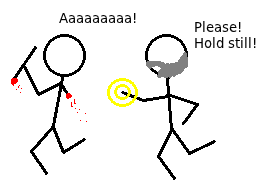
\includegraphics{Pics/Regenerate.png}
\end{figure*}

The subject's severed body members (fingers, toes, hands, feet, arms, legs, tails, or even heads of multiheaded creatures), broken bones, and ruined organs grow back. 
After the spell is cast, the physical regeneration is complete in 1 round if the severed members are present and touching the creature. It takes 2d10 rounds otherwise.
This regeneration is instantaneous in nature.

Regenerate also grants the subject Fast Healing 3 for 1 minute, rids the subject of \emph{exhaustion} and/or \emph{fatigue}, and eliminates all nonlethal damage the subject has taken.
It has no effect on nonliving creatures (including undead).

\paragraph{Augment:} If you spend 2 additional spell points and 200XP, you can target this spell on the remains of a creature that has been dead for no longer than 1 round.
The creature then immediately comes back to life, at -9 hit points. It suffers no level loss, loss of constitution, or other usual drawbacks of dying, since this spell acts before the subject's soul has fully left the body.
If the creature's remains were in a especially bad state (such as due to death by decapitation, or a \nameref{Spell:Disintegrate} or \nameref{Spell:Implosion} spell), it takes 2d10 rounds for the creature to reform its body, during which time it cannot act.
Even if the subject's remains were mostly intact and its hit points are brought into the positives, it cannot act for one round after being brought back to life in this way, since the spell needs time to repair the lethal damage.
The spell's other functions affect the creature normally. It gains Fast Healing 3 for 1 minute, and is cured of all \emph{exhaustion}, \emph{fatigue}, and nonlethal damage.
\subsubsection{Reincarnate}
\label{Spell:Reincarnate}
Necromancy (Healing)
\\ \textbf{Level:} Chaos 4
\\ \textbf{Components:} V, S
\\ \textbf{Casting Time:} 1 minute
\\ \textbf{Range:} Touch
\\ \textbf{Target:} Dead creature touched
\\ \textbf{Duration:} Instantaneous
\\ \textbf{Saving Throw:} None; see text
\\ \textbf{Spell Resistance:} Yes (harmless)
\\ \textbf{Spell Points:} 7; XP; see text

\emph{''This body is finished. But I can create a new one.``}

You restore life to a deceased creature by creating a new body for it. 
You can raise a creature that has been dead for no longer than one week. 
In addition, the subject's soul must be free and willing to return. 
If the subject's soul is not willing to return, the spell does not work; 
therefore, a subject that wants to return receives no saving throw.

Since the dead creature is returning in a new body, all physical ills and afflictions are repaired 
(including ability damage, ability drain, as well as normal disease and poison, but not curses or magical diseases).
The condition of the remains is not a factor.
So long as some small portion of the creature's body still exists, 
it can be reincarnated, but the portion receiving the spell must have been part of the creature's body at the time of death. 
The magic of the spell creates an entirely new body (of an age category equal to that of the subject's previous body) 
for the soul to inhabit from the natural elements at hand.
The new body may be of a race different from the creature's original.
This process takes 1 hour to complete. When the body is ready, the subject is reincarnated.
A reincarnated creature has a number of hit points equal to its current Hit Dice.
None of the dead creature's equipment or possessions are affected in any way by this spell.

Coming back from the dead is an ordeal. 
The subject of the spell loses one level (or 1 Hit Die) when it is raised, 
just as if it had lost a level or a Hit Die to an energy-draining creature. 
If the subject is 1st level, 
it loses 2 points of Constitution instead (if this would reduce its Con to 0 or less, it can't be raised). 
This level/HD loss or Constitution loss cannot be repaired by any means (if the character's race changes, determine its ability score changes first). 
A character who died with unused spell points comes back with 50\% of them (rounded down, minimum 0).
The potential spell point loss for losing a level won't come in until the next time the raised character replenishes his spell points.

A creature who has been turned into an undead creature or killed by a death effect can't be raised by this spell. 
Constructs, elementals, outsiders, and undead creatures can't be raised. 
The spell cannot bring back a creature that has died of old age.

To determine the race of the creature's new body, roll on the \nameref{tab:Reincarnate} table.
%For a humanoid creature, the new incarnation is determined using reincarnate table. 
%For nonhumanoid creatures, a similar table of creatures of the same type should be created. 
Whatever the result, a Reincarnate spell can never result in a creature's level adjustment or number of hit dice
(aside from level loss, see above) changing.
\begin{tableonecolumn}
\caption{Reincarnate}
\label{tab:Reincarnate}
\begin{tabular}{|l|l|}
\hline
d\%&Incarnation\\
\hline
$\leq$5&Caster's race\\
6-10&Target's choice (other than old race)\\
11-40&Same as old race\\
41-50&Related race (GM's adjucation)\\
51-60&Decidedly unrelated race (GM's adjucation)\\
61-90&Roll randomly among races in the setting\\
91+&GM's choice\\
\hline
\end{tabular}
\end{tableonecolumn}
To determine the ability scores of a reincarnated creature, eliminate its old racial adjustments to ability scores,
and add the racial adjustments of its new race (including mental ability scores).
The reincarnated creature gains all abilities associated with its new form, 
including forms of movement and speeds, natural armor, natural attacks, extraordinary abilities, and the like, 
but it doesn't automatically speak the language of the new form. 

If the subject's race changes, it hereafter ages as a creature of its new race.
For example, an orc that reached middle age just before being reincarnated as an elf ages from that point as any other elf
that just reached middle age (even if the character's absolute age would not even place it as an adult for naturally born elves).
For venerable creatures, reroll the maximum age according to its new race.

\paragraph{Augment:} This spell can be augmented in one or more of the following ways:
\begin{enumerate}
 \item If you spend 2 additional spell points and 500 additional XP, 
the creature can have been dead no longer than 10 years per caster level rather than one week.
 \item If you spend an additional spell point and 250 additional XP, a spellcaster being raised does not
lose any spell points as part of returning from the dead.
 \item If you spend an additional spell point and 250 additional XP, 
curses and magical diseases are cured as part of the subject returning from the dead.
 \item If you spend 2 additional spell points and 250 additional XP, 
you can reincarnate someone killed by a death effect.
 \item If you spend 8 additional spell points and 4000 additional XP,
the subject of the spell does not lose a level or points of constitution (other than due to a change in the subject's race) when it is reincarnated.
\end{enumerate}

\emph{Experience Cost:} 200XP.
\subsubsection{Remove Blindness/Deafness}
\label{Spell:RemoveBlindnessDeafness}
Necromancy (Healing)
\\ \textbf{Level:} Paladin 3
\\ \textbf{Components:} V, S
\\ \textbf{Casting Time:} 1 standard action
\\ \textbf{Range:} Touch
\\ \textbf{Target:} Creature touched
\\ \textbf{Duration:} Instantaneous
\\ \textbf{Saving Throw:} Fortitude negates (harmless)
\\ \textbf{Spell Resistance:} Yes (harmless)
\\ \textbf{Spell Points:} 5

\emph{''No, my good man, it's really not a Miracle. Just the cure for blindness.``}

This spell cures blindness, deafness, or damage to or loss of any one special sense (such as scent, blindsight, blindsense, or tremorsense). 
Whether the effect is normal or magical in nature does not matter.
The spell does not restore ears or eyes that have been lost, but it repairs them if they are damaged.
\subsubsection{Remove Curse}
\label{Spell:RemoveCurse}
Abjuration
\\ \textbf{Level:} Bard 3, Healing 3, Luck 3, Paladin 3, Sor/Wiz 4
\\ \textbf{Components:} V, S
\\ \textbf{Casting Time:} 1 minute
\\ \textbf{Range:} Touch
\\ \textbf{Target:} Creature or item touched
\\ \textbf{Duration:} Instantaneous
\\ \textbf{Saving Throw:} Will negates (harmless)
\\ \textbf{Spell Resistance:} Yes (harmless)
\\ \textbf{Spell Points:} Bard 5, Healing 5, Luck 5, Paladin 5, Sor/Wiz 7

\emph{Many magical maladies exist, and this is the cure for most of them.}

Remove curse instantaneously removes all curses on an object or a creature. 
Remove curse does not remove the curse from a cursed shield, weapon, or suit of armor, although the spell typically enables the creature afflicted with any such cursed item to remove and get rid of it. 
Certain special curses may not be countered by this spell or may be countered only by a caster of a certain level or higher.

\paragraph{Augment:} If you spend 2 additional spell points, the spell can free victims from enchantments and transmutations in addition to curses.
The spell can then reverse even an instantaneous effect.
For each such effect, you make a caster level check (1d20 + caster level) against a DC of 11 + caster level of the effect.
Success means that the creature is free of the spell, curse, or effect. For a cursed magic item, the DC is 25.

If the spell to be removed is one that cannot be dispelled by \nameref{Spell:DispelMagic}, this spell works only if that spell was cast using fewer spell points than were spent on casting this spell.
\subsubsection{Remove Disease}
\label{Spell:RemoveDisease}
Necromancy (Healing)
\\ \textbf{Level:} Healing 3, Paladin 3, Ranger 3
\\ \textbf{Components:} V, S
\\ \textbf{Casting Time:} 1 standard action
\\ \textbf{Range:} Touch
\\ \textbf{Target:} Creature touched
\\ \textbf{Duration:} Instantaneous
\\ \textbf{Saving Throw:} Fortitude negates (harmless)
\\ \textbf{Spell Resistance:} Yes (harmless)
\\ \textbf{Spell Points:} 5

\emph{''Plague? No problem.``}

Remove disease cures all diseases that the subject is suffering from. 
The spell also kills parasites, including green slime and others. 
Certain special diseases may not be countered by this spell or may be countered only by a caster of a certain level or higher.

\emph{Note:} Since the spell's duration is instantaneous, it does not prevent reinfection after a new exposure to the same disease at a later date.
\subsubsection{Remove Fear}
\label{Spell:RemoveFear}
Abjuration
\\ \textbf{Level:} Bard 1, Healing 1, Paladin 1
\\ \textbf{Components:} V, S
\\ \textbf{Casting Time:} 1 standard action
\\ \textbf{Range:} Touch
\\ \textbf{Targets:} One creature
\\ \textbf{Duration:} 1 round/level
\\ \textbf{Saving Throw:} Will negates (harmless)
\\ \textbf{Spell Resistance:} Yes (harmless)
\\ \textbf{Spell Points:} 1

\emph{Your fear does not go anywhere. But it no longer impedes you.}

The subject gains immunity to fear effects.

\paragraph{Augment:} You can augment this spell in one or both of the following ways:
\begin{enumerate}
 \item For every three additional spell points you spend, this spell can affect an additional creature.
 \item If you spend 2 additional spell points, the spell's duration increases to 10 minutes per level.
\end{enumerate}
\subsubsection{Remove Paralysis}
\label{Spell:RemoveParalysis}
Conjuration (Healing)
\\ \textbf{Level:} Healing 2
\\ \textbf{Components:} V, S
\\ \textbf{Casting Time:} 1 standard action
\\ \textbf{Range:} Close (25 ft. + 5 ft./2 levels)
\\ \textbf{Target:} One creature
\\ \textbf{Duration:} Instantaneous
\\ \textbf{Saving Throw:} Will negates (harmless)
\\ \textbf{Spell Resistance:} Yes (harmless)
\\ \textbf{Spell Points:} 3

\emph{''Stand up! It's just paralysis!``}

You can free one creature from the effects of any temporary \emph{paralysis} or related magic, including a ghoul's touch or a \nameref{Spell:Slow} spell. It does not heal creatures who have been permanently paralyzed in mundane circumstances (such creatures who have taken spinal damage).

The spell does not restore ability scores reduced by penalties, damage, or drain.

\paragraph{Augment:} You can augment this spell in one or both of the following ways:
\begin{enumerate}
 \item For every two additional spell points you spend, this spell can affect an additional creature.
No two recipients of the spell may be more than 30' apart. 
 \item If you spend 10 additional spell points, you can heal mundane paralysis.
\end{enumerate}
\subsubsection{Repair}
\label{Spell:Repair}
Transmutation
\\ \textbf{Level:} Bard 1, Sor/Wiz 1
\\ \textbf{Components:} V, S
\\ \textbf{Casting Time:} 1 standard action
\\ \textbf{Range:} Touch
\\ \textbf{Target:} One object of up to 1 lb./level OR construct touched; See text
\\ \textbf{Duration:} Instantaneous
\\ \textbf{Saving Throw:} Will negates (harmless)
\\ \textbf{Spell Resistance:} Yes (harmless)
\\ \textbf{Spell Points:} 1, XP; see text

\emph{''Reparo!``}

The spell has two separate functions, \emph{Mending} (which affects items) and \emph{Repair construct} (which affects constructs). 
Each has its own usage descriptions and augmentation options.
\begin{list}{\labelitemi}{\leftmargin=1em}
 \item \emph{Mending:} This function of the spell repairs breaks or tears in objects, making it strong as new. 
It will completely repair broken objects up to its weight limit, regardless of the number of breaks, so long as all the pieces are present.
The spell can repair a magic item, but the item's magical abilities are not restored. 
The spell cannot mend broken magic rods, staffs, or wands,

\paragraph{Augment:} You can Augment the Mending function of the spell in one of the following ways:
\begin{enumerate}
 \item If you spend two additional spell points, the weight limit of the spell increases to 10 lb./level.
 \item If you spend six additional spell points, the weight limit of the spell increases to 100 lb./level.
 \item If you spend eight additional spell points, the spell restores the magical abilities of a broken magic item when it repairs such an item.
 It can mend broken magic rods, staffs and wands, restoring their status to what it was at the time the item was broken. It never restores spent charges.
 \item If you spend sixteen additional spell points, the spell can restore the magical properties of a magic item (other than an artifact) that
 has been drained of magic by a \nameref{Spell:Disjunction} spell. 
 This use of the spell requires you to expend a number of experience points equal to the number required to craft the item in the first place.
\end{enumerate}
\item \emph{Repair Construct:} When laying your hands upon a construct that has at least 1 hit point remaining, 
you reknit its structure to repair damage it has taken. 
The spell repairs 1d8 points of damage +1 point per caster level. 
Constructs that are immune to magic cannot be repaired in this fashion.

\paragraph{Augment:} For every 2 additional spell points you spend, the Repair construct function of the spell repairs an additional 1d8 points of damage.
\end{list}
\subsubsection{Repel Metal and Stone}
\label{Spell:RepelMetalAndStone}
Abjuration [Earth]
\\ \textbf{Level:} Earth 8
\\ \textbf{Components:} V, S
\\ \textbf{Casting Time:} 1 standard action
\\ \textbf{Range:} 60 ft.
\\ \textbf{Area:} 60-ft. line from you
\\ \textbf{Duration:} 1 round/level (D)
\\ \textbf{Saving Throw:} None
\\ \textbf{Spell Resistance:} No
\\ \textbf{Spell Points:} 15

\emph{Waves of invisible and intangible energy roll forth from you.}

All metal or stone objects in the path of the spell are pushed away from you to the limit of the range. 
Fixed metal or stone objects larger than 3 inches in diameter and loose objects weighing more than 500 pounds are not affected. 
Anything else, including animated objects, small boulders, and creatures in metal armor, moves back. 
Fixed objects 3 inches in diameter or smaller bend or break, and the pieces move with the wave of energy. 
Objects affected by the spell are repelled at the rate of 40 feet per round.

Objects such as metal armor, swords, and the like are pushed back, dragging their bearers with them. A creature being dragged by an item it is carrying can let go. A creature being dragged by a shield can loose it as a move action and drop it as a free action.
Even magic items with metal components are repelled.

After you cast the spell, its area and direction path are set, and you can then do other things or go elsewhere without affecting the spell's power.

\paragraph{Augment:} If you spend 2 additional spell points, this spell's range changes to 10', and its area changes to a 10' radius emanation, centered on you.
The spell then follows you around, remaining centered on you for the duration.
\subsubsection{Repel Vermin}
\label{Spell:RepelVermin}
Abjuration
\\ \textbf{Level:} Bard 4, Ranger 4, Vermin 4
\\ \textbf{Components:} V, S
\\ \textbf{Casting Time:} 1 standard action
\\ \textbf{Range:} 10 ft.
\\ \textbf{Area:} 10-ft.-radius emanation centered on you
\\ \textbf{Duration:} 10 min./level (D)
\\ \textbf{Saving Throw:} None or Will negates; see text
\\ \textbf{Spell Resistance:} Yes
\\ \textbf{Spell Points:} 7

\emph{You create an invisible barrier to hold back vermin.} 

A vermin with 3 Hit Dice or less cannot enter within the radius of the emanation. 
This includes all swarms consisting of vermin, regardless of the swarm's total number of Hit Dice.

A vermin with more than 3 Hit Dice can penetrate the barrier if it succeeds on a Will save. 
Even so, crossing the barrier deals the vermin 2d6 points of damage, and pressing against the barrier causes pain, which deters most vermin.

\paragraph{Augment:} For every 2 additional spell points you spend, the emanation prevents the entry of creatures with one additional Hit Die, and the damage dealt to higher HD vermin who manage to cross is increased by one die (d6).
\subsubsection{Repel Wood}
\label{Spell:RepelWood}
Abjuration [Earth]
\\ \textbf{Level:} Plant 6, Ranger 6
\\ \textbf{Spell Points:} 11

\emph{Waves of warm energy softly emanate out from your position.}

This spell functions as \nameref{Spell:RepelMetalAndStone} (including its augmentation option), except as noted here, and it affects objects made of wood (such as wooden shields, spears, wooden weapon shafts and hafts, and arrows and bolts), rather than objects of metal and stone.

\subsubsection{Repelling Light}
\label{Spell:RepellingLight}
Abjuration [Light]
\\ \textbf{Level:} Sun 4
\\ \textbf{Components:} V, S
\\ \textbf{Casting Time:} 1 standard action
\\ \textbf{Range:} 10 ft.
\\ \textbf{Area:} 10-ft.-radius emanation centered on you
\\ \textbf{Duration:} 1 round/level (D)
\\ \textbf{Saving Throw:} Will negates; see text
\\ \textbf{Spell Resistance:} Yes
\\ \textbf{Spell Points:} 7

\emph{I am a servant of the Secret Fire, wielder of the flame of Anor. The dark fire will not avail you, flame of Udûn. Go back to the Shadow! You cannot pass.} 

You bring into being a mobile, globe of light that prevents the entrance of many types of foul creatures.
The globe moves around with you.

The effect hedges out evil outsiders, undead creatures, natives of the plane of shadow, and creatures who take damage or penalties from bright light or sunlight. A creature of the listed types can penetrate the barrier if it succeeds on a Will save. 
Even so, crossing the barrier deals the creature 2d6 points of damage.

This spell may be used only defensively, not aggressively. Forcing the globe against a creature that the spell keeps at bay lets the creature in (without dealing damage), and prevents the spell from affecting it again until it exits the emanation and attempts to re-enter.

Creatures with reach sufficient to stand outside the globe and attack the caster can do so, even with natural weapons (the globe does not do its work instantaneously).

The spell's area is illuminated to the point of bright illumination. In addition, shadowy illumination extends out to twice the spell's listed radius.
If an area of magical light and an area of magical darkness overlap, the spell on which more spell points were spent prevails.
If an equal number of spell points were spent on both spells, ambient light conditions remain.

\paragraph{Augment:} You can augment this spell in one or both of the following ways.
\begin{enumerate}
 \item For every 4 additional spell points you spend, the globe's range and radius increases by 5'.
 \item If you spend 4 additional spell points, creatures that attempt to move into the spell's area are \emph{blown away} from the caster if they fail the will save.
\end{enumerate}


\subsubsection{Resilient Sphere}
\label{Spell:ResilientSphere}
Evocation [Force]
\\ \textbf{Level:} Evoker 4
\\ \textbf{Components:} V, S
\\ \textbf{Casting Time:} 1 standard action
\\ \textbf{Range:} Close (25 ft. + 5 ft./2 levels)
\\ \textbf{Effect:} Sphere of force, centered around a medium-sized or smaller creature
\\ \textbf{Duration:} 1 min./level (D)
\\ \textbf{Saving Throw:} Reflex negates
\\ \textbf{Spell Resistance:} Yes
\\ \textbf{Spell Points:} 7

\emph{''You're not going anywhere.``}

A globe of shimmering, transparent force encloses a creature of size medium or smaller. 
The sphere contains its subject for the spell's duration. 
The sphere is not subject to damage of any sort except from a rod of cancellation, 
a rod of negation, a \nameref{Spell:Disintegrate} spell, or a targeted \nameref{Spell:DispelMagic} spell. 
These effects destroy the sphere without harm to the subject. 
Nothing can pass through the sphere, inside or out, though the subject can breathe normally.

The subject may struggle, but the sphere cannot be physically moved either by people outside it or by the struggles of those within.

\paragraph{Augment:} You can augment this spell in one or more of the following ways.

\begin{enumerate}
 \item If you spend 6 additional spell points, this spell does not offer a saving throw.
 \item For every 3 additional spell points you spend, this spell can affect a creature one size category larger than medium.
 \item If you spend 6 additional spell points, 
you can telekinetically move the sphere as long as its contents weigh 5,000 pounds or less. 
The telekinetic control extends from you out to medium range (100 feet + 10 feet per caster level) after the sphere has succeeded in encapsulating its contents.
You can move objects or creatures in the sphere that weigh a total of 5,000 pounds or less by concentrating on the sphere. 
You can begin moving a sphere in the round after casting the spell. 
If you concentrate on doing so (a standard action), you can move the sphere as much as 30 feet in a round. 
If you cease concentrating, the sphere does not move in that round (if on a level surface) or descends at its falling rate (if aloft) until it reaches a level surface, 
or the spell's duration expires, or you begin concentrating again. 
If you cease concentrating (voluntarily or due to failing a Concentration check), you can resume concentrating on your next turn or any later turn during the spell's duration.

The sphere falls at a rate of only 60 feet per round, which is not fast enough to cause damage to the contents of the sphere.

You can move the sphere telekinetically even if you are in it. 
\end{enumerate}
\subsubsection{Resistance}
\label{Spell:Resistance}
Abjuration
\\ \textbf{Level:} Abjurer 2, Blackguard 2, Paladin 2, Protection 2, Ranger 2
\\ \textbf{Components:} V, S
\\ \textbf{Casting Time:} 1 standard action
\\ \textbf{Range:} Touch
\\ \textbf{Target:} Creature touched
\\ \textbf{Duration:} 10 min./level
\\ \textbf{Saving Throw:} Will negates (harmless)
\\ \textbf{Spell Resistance:} Yes (harmless)
\\ \textbf{Spell Points:} 3

\emph{You defend the subject with the most general of abjurations.}

This spell grants a +1 resistance bonus on saving throws.

\paragraph{Augment:} You can augment this spell in one or both of the following ways.
\begin{enumerate}
\item For every three additional spell points you spend, the resistance bonus increases by 1.
\item If you spend two additional spell points, the spell's duration increases to 24 hours.
\end{enumerate}

\subsubsection{Resist Energy}
\label{Spell:ResistEnergy}
Abjuration
\\ \textbf{Level:} Blackguard 2, Fire 2, Paladin 2, Ranger 2, Sor/Wiz 2
\\ \textbf{Components:} V, S
\\ \textbf{Casting Time:} 1 standard action
\\ \textbf{Range:} Touch
\\ \textbf{Target:} Creature touched
\\ \textbf{Duration:} 10 min./level
\\ \textbf{Saving Throw:} Will negates (harmless)
\\ \textbf{Spell Resistance:} Yes (harmless)
\\ \textbf{Spell Points:} 3

\emph{Suddenly, the elements no longer seem all that frightening.}

The subject of this spell gains resistance 10 against acid, cold, electricity, fire or sonic damage, chosen at the time of casting.

The energy resistance provided by this spell increases to 20 points at caster level 9th, and to its maximum of 30 at 13th level.
The spell protects equipment as well.

\paragraph{Augment:} You can augment this spell in one or both of the following ways.
\begin{enumerate}
\item If you spend four additional spell points, the subject gains resistance to all the listed energy types, rather than just one.
\item If you spend four additional spell points, you can cast this spell as an immediate action.
\end{enumerate}
\subsubsection{Restoration}
\label{Spell:Restoration}
Necromancy (Healing)
\\ \textbf{Level:} Healing 2, Paladin 2
\\ \textbf{Components:} V, S
\\ \textbf{Casting Time:} 3 rounds
\\ \textbf{Range:} Touch
\\ \textbf{Target:} Creature touched
\\ \textbf{Duration:} Instantaneous
\\ \textbf{Saving Throw:} Will negates (harmless)
\\ \textbf{Spell Resistance:} Yes (harmless)
\\ \textbf{Spell Points:} 3

\emph{The creature breathes more easily.}

Restoration dispels any magical effects reducing one of the subject's ability scores or cures 1d4 points of temporary ability damage to one of the subject's ability scores. 
It also eliminates any fatigue suffered by the character, and improves an exhausted condition to fatigued. 
It does not restore permanent ability drain.

\paragraph{Augment:} You can augment this spell in one or more of the following ways:
\begin{enumerate}
 \item If you spend 4 additional spell points, this spell also dispels negative levels and restores one experience level to a creature who has had a level drained. The drained level is restored only if the time since the creature lost the level is equal to or less than one day per caster level. 
A character who has a level restored by restoration has exactly the minimum number of experience points necessary to restore him or her to his or her previous level.
This augment does not restore levels or Constitution points lost due to death.
 \item If you spend 4 additional spell points, this spell cures all temporary ability damage, and it restores all points permanently drained from a single ability score (your choice if more than one is drained). 
It also eliminates any fatigue or exhaustion suffered by the target.
 \item If you spend 10 additional spell points and 500XP, this spell removes all forms of insanity, confusion, and similar mental effects.
\end{enumerate}
\subsubsection{Reverse Gravity}
\label{Spell:ReverseGravity}
Abjuration
\\ \textbf{Level:} Sor/Wiz 7, Travel 7
\\ \textbf{Components:} V, S
\\ \textbf{Casting Time:} 1 standard action
\\ \textbf{Range:} Medium (100 ft. + 10 ft./level)
\\ \textbf{Target:} One creature
\\ \textbf{Duration:} Instantaneous
\\ \textbf{Saving Throw:} None
\\ \textbf{Spell Resistance:} Yes
\\ \textbf{Spell Points:} 13

\emph{''Enjoy your flight.``}

You change the way gravity affects the target creature.
The creature instantaneously ''falls'' 500' in any direction (other than down).
This fall is treated as an ordinary fall in all respects - the target takes the appropriate falling damage if it hits something on the way (such as the ceiling),
the \nameref{Spell:ControlFall} spell makes it fall 60' rather than 500', a creature with a Fly speed is not affected unless it wishes to, 
and the target (or those near to it) may use the Climb skill to catch itself as it falls.

Reality rapidly compensates for this breach of the laws of physics, making traditional ballistics inapplicable.\footnote{\emph{Optional rule:}
Ballistics apply. Rather than ``falling 500''', the effects of gravity on the subject are ignored for one round, and a force with an equal magnitude
but different direction is applied to the subject for the same duration. 
This approach is recommended only if someone at the table has a talent for on-the-fly vector calculus.}
If you cause the creature to fall at an angle, 
refer to the \nameref{tab:ReverseGravity} table for a reference on the vertical and horizontal distances the subject falls.
\begin{tableonecolumn}
\caption{Reverse Gravity Angle Examples}
\label{tab:ReverseGravity}
\begin{tabular}{|r|r|r|}
\hline
Angle$^1$&Horizontal&Maximum\\
&distance$^2$&height$^2$\\
\hline
 0$^\circ$&500 feet&  0 feet\\
15$^\circ$&485 feet&130 feet\\
30$^\circ$&435 feet&250 feet\\
45$^\circ$&355 feet&355 feet\\
60$^\circ$&250 feet&435 feet\\
75$^\circ$&130 feet&485 feet\\
90$^\circ$&  0 feet&500 feet\\
\hline
\multicolumn{3}{p{5cm}}{\small $^1$ An angle with respect to the ground the creature was standing on.}\\
\multicolumn{3}{p{5cm}}{\small $^2$ With respect to the ground the creature was standing on.}
\end{tabular}
\end{tableonecolumn}
A creature always falls straight down after travelling 500' in this fashion.

\paragraph{Augment:} For every 2 additional spell points you spend, this spell affects an additional creature within range.
\subsubsection{Righteous Might}
\label{Spell:RighteousMight}
Transmutation [see text]
\\ \textbf{Level:} Blackguard 5, Paladin 5, Strength 5, War 5
\\ \textbf{Components:} V, S
\\ \textbf{Casting Time:} 1 standard action
\\ \textbf{Range:} Personal
\\ \textbf{Target:} You
\\ \textbf{Duration:} 1 round/level (D)
\\ \textbf{Spell Points:} 9

\emph{``By the power of Greyskull!''}

\begin{figure*}
  \caption{Cleric uses Righteous Might to match the combat prowess of a superior foe.}
  \centering
    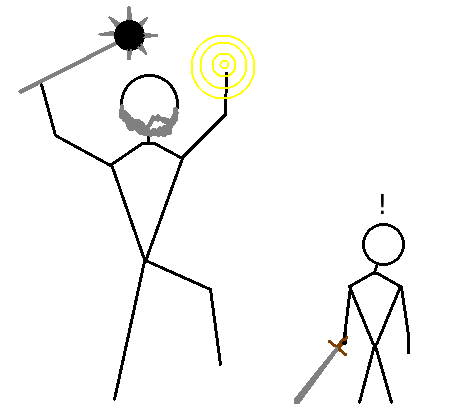
\includegraphics{Pics/RighteousMight.png}
\end{figure*}

Your height is doubled, your weight is multiplied by 8, and your size category increases to the next larger one.
You gain a +4 size bonus to Strength, a +2 size bonus to Constitution, 
and your size modifier for AC and attacks changes as appropriate to your new size category.
You gain a +2 enhancement bonus to your natural armor.
At the time you cast this spell, choose an alignment you wish to protect yourself against.
You gain DR 3/that alignment. The spell gains a descriptor opposed to that alignment
(for example, if you choose to gain DR/evil, this becomes a Transmutation [Good] spell).

A humanoid creature whose size increases to Large has a space of 10 feet and a natural reach of 10 feet.
If insufficient room is available for the desired growth, 
you attain the maximum possible size and may make a Strength check 
(using your increased Strength) to burst any enclosures in the process. 
If the check fails, you are constrained without harm by the materials enclosing you - 
you cannot crush yourself by increasing your size.

This spell does not change your speeds.

All equipment worn or carried by you has its size similarly altered by the spell. 
See Table: Larger and Smaller Weapon Damage for effects on the damage of weapons.
Note the effects of your changed carrying capacity.
Any item that leaves your possession while you have had your size altered (including a projectile or thrown weapon) 
instantly returns to its normal size. 
This means that thrown weapons deal their normal damage, and projectiles deal damage based on the size of the weapon that fired them. 

\paragraph{Augment:} If you spend 6 additional spell points, 
your height is tripled, your weight is multiplied sixteenfold, 
and your size category increases by two instead of one.
You instead gain a +6 size bonus to Strength, and a +3 enhanchement bonus to your natural armor.

In addition, for every additional spell point you spend, 
the damage reduction offered by this spell increases by 1.

\subsubsection{Rusting Grasp}
\label{Spell:RustingGrasp}
Transmutation
\\ \textbf{Level:} Destruction 4, Water 4
\\ \textbf{Components:} V, S
\\ \textbf{Casting Time:} 1 standard action
\\ \textbf{Range:} Touch
\\ \textbf{Target:} One nonmagical ferrous object (or the volume of the object within 3 ft. of the touched point) or one ferrous creature
\\ \textbf{Duration:} See text
\\ \textbf{Saving Throw:} None
\\ \textbf{Spell Resistance:} No
\\ \textbf{Spell Points:} 7

\emph{``An Iron Golem, you say? I have just the thing.''}

Any iron or iron alloy item you touch becomes instantaneously rusted, pitted, and useless. If the item is so large that it cannot fit within a 3-foot radius a 3-foot-radius volume of the metal is rusted and destroyed. Magic items made of metal are immune to this spell.
Provided all the rusted remains are present, a \nameref{Spell:Repair} spell can restore an item to its former status.

You may employ rusting grasp in combat with a successful melee touch attack. Rusting grasp used in this way instantaneously destroys 1d6 points of Armor Class gained from metal armor (to the maximum amount of protection the armor offered) through corrosion.

Weapons in use by an opponent targeted by the spell are more difficult to grasp. You must succeed on a melee touch attack against the weapon. A metal weapon that is hit is destroyed.
Striking at an opponent's weapon in this way provokes an attack of opportunity unless you have the Improved Sunder feat. Also, you must touch the weapon and not the other way around.

Against a ferrous creature, rusting grasp instantaneously deals 7d6 points of damage per successful attack. 

The spell lasts for 1 round per level, and you can make one melee touch attack per round.

\paragraph{Augment:} If you spend 2 additional spell points, magic items made of metal are not immune to this spell.
\subsection{'S' Spells}
\subsubsection{Sanctuary}
\label{Spell:Sanctuary}
Abjuration
\\ \textbf{Level:} Protection 1
\\ \textbf{Components:} V, S,
\\ \textbf{Casting Time:} 1 standard action
\\ \textbf{Range:} Touch
\\ \textbf{Target:} Creature touched
\\ \textbf{Duration:} 1 round/level
\\ \textbf{Saving Throw:} Will negates
\\ \textbf{Spell Resistance:} No
\\ \textbf{Spell Points:} 1

\emph{You take the fundamental injustice involved when a violent man attacks an innocent, and turn it into a shield.}

Any opponent attempting to strike or otherwise directly attack the warded creature, even with a targeted spell, must attempt a Will save. 
If the save succeeds, the opponent can attack normally and is unaffected by that casting of the spell. 
If the save fails, the opponent can't follow through with the attack, that part of its action is lost, and it can't directly attack the warded creature for the duration of the spell. 
Those not attempting to attack the subject remain unaffected. 
This spell does not prevent the warded creature from being attacked or affected by area or effect spells. 
The subject cannot attack without breaking the spell but may use nonattack spells or otherwise act.

\paragraph{Augment:} If you spend 10 additional spell points, this spell's duration increases to 24 hours.
\subsubsection{Scorching Ray}
\label{Spell:ScorchingRay}
Evocation [see text]
\\ \textbf{Level:} Sor/Wiz 1
\\ \textbf{Components:} V, S
\\ \textbf{Casting Time:} 1 standard action
\\ \textbf{Range:} Close (25 ft. + 5 ft./2 levels)
\\ \textbf{Effect:} Ray
\\ \textbf{Duration:} Instantaneous
\\ \textbf{Saving Throw:} None
\\ \textbf{Spell Resistance:} Yes
\\ \textbf{Spell Points:} 1

\emph{This simplest of evocations remains as one as the most reliable.}

At the time of casting, you choose between cold, electricity, fire, or sonic damage. 

You create a ray of energy of the chosen type that shoots forth from your fingertip and strikes a target within range, 
dealing 1d6 points of damage, if you succeed on a ranged touch attack with the ray.

\begin{list}{\labelitemi}{\leftmargin=1em}
 \item Cold: A ray of this energy type deals +1 point of damage per die.
 \item Electricity: Casting a ray of this energy type provides a +3 bonus on your attack roll if the target is wearing metal armor 
 and a +2 bonus on caster level checks for the purpose of overcoming spell resistance.
 \item Fire: A ray of this energy type deals +1 point of damage per die. (This was the form of the spell that was discovered first among Evokers.
 Although further research showed that the same spell could produce the other energy types with minimal modifications, the name of ''scorching ray`` stuck.)
 \item Sonic: A ray of this energy type deals -1 point of damage per die and ignores an object's hardness.
\end{list}

This spell's descriptor is the same as the type of energy you selected. 

\paragraph{Augment:} For every additional spell point you spend, this spell's damage increases by one die (d6).
\subsubsection{Screen}
\label{Spell:Screen}
Illusion (Glamer)
\\ \textbf{Level:} Illusionist 8, Trickery 7
\\ \textbf{Components:} V, S
\\ \textbf{Casting Time:} 10 minutes
\\ \textbf{Range:} Close (25 ft. + 5 ft./2 levels)
\\ \textbf{Area:} 30-ft. cube/level (S)
\\ \textbf{Duration:} 24 hours
\\ \textbf{Saving Throw:} None or Will disbelief (if interacted with); see text
\\ \textbf{Spell Resistance:} No
\\ \textbf{Spell Points:} Illusionist 15, Trickery 13

\emph{This spell combines several elements to create a powerful protection from scrying and direct observation. }

When casting the spell, you dictate what will and will not be observed in the spell's area. 
The illusion created must be stated in general terms. Once the conditions are set, they cannot be changed.

Attempts to scry the area automatically detect (do not penetrate) the image stated by you with no save allowed. 
Sight and sound are appropriate to the illusion created.

Direct observation may allow a save (as per a normal illusion), 
if there is cause to disbelieve what is seen. 
Even entering the area does not cancel the illusion or necessarily allow a save, 
assuming that hidden beings take care to stay out of the way of those affected by the illusion. 
\subsubsection{Scrying}
\label{Spell:Scrying}
Divination (Scrying)
\\ \textbf{Level:} Bard 3, Diviner 4, Knowledge 4
\\ \textbf{Components:} V, S
\\ \textbf{Casting Time:} 1 hour
\\ \textbf{Range:} See text
\\ \textbf{Effect:} Magical sensor next to a creature
\\ \textbf{Duration:} 1 min./level
\\ \textbf{Saving Throw:} Will negates
\\ \textbf{Spell Resistance:} Yes
\\ \textbf{Spell Points:} Bard 5, Diviner 7, Knowledge 7

\emph{Distances suddenly mean very little to your ability to glean information.}

You can see and hear some creature, which may be at any distance. 
If the subject succeeds on a Will save, the scrying attempt simply fails. 
The difficulty of the save depends on how well you know the subject and what sort of physical connection (if any) you have to that creature (see the \nameref{tab:Scrying} table). 

If the save fails, you can see and hear the subject and the subject's immediate surroundings (approximately 10 feet in all directions of the subject). 
If the subject moves, the scrying sensor follows, regardless of its speed.
If it uses a teleportation spell to move more than 10 feet or crosses planar boundaries, however, the spell ends.

The sensor has your full visual acuity, including any magical effects. %In addition, 
%the following spells have a 5\% chance per caster level of operating through the sensor: 
%detect chaos, detect evil, detect good, detect law, detect magic, and message.

If the save succeeds, you can't attempt to scry on that subject again for 24 hours.

\begin{table*}
\caption{Scrying save modifiers}
\label{tab:Scrying}
\begin{center}
\begin{tabular}{|l|c|}
\hline
Knowledge & Will Save Modifier$^1$\\
\hline
None$^2$&+10\\
Secondhand (you have heard of the subject)&+5\\
Firsthand (you have met the subject)&+0\\
Familiar (you know the subject well)&-5\\
\hline
Connection&Will Save Modifier\\
\hline
Likeness or picture&-2\\
Possession or garment&-4\\
Body part, lock of hair, bit of nail, etc.&-10\\
Subject is on another plane&+5\\
\hline
\multicolumn{2}{l}{\small $^1$Modifiers are cumulative.}\\
\multicolumn{2}{l}{\small $^2$You must have some sort of connection to a creature you have no knowledge of.}\\
\end{tabular}
\end{center}
\end{table*}

\paragraph{Augment:} If you spend 6 additional spell points, you can cast this spell as a standard action.
\subsubsection{Searing Blade}
\label{Spell:SearingBlade}
Evocation [Light]
\\ \textbf{Level:} Paladin 2
\\ \textbf{Components:} V, S
\\ \textbf{Casting Time:} 1 swift action
\\ \textbf{Range:} Touch
\\ \textbf{Target:} Weapon touched
\\ \textbf{Duration:} 1 round; See text
\\ \textbf{Saving Throw:} None
\\ \textbf{Spell Resistance:} Yes
\\ \textbf{Spell Points:} 3

\emph{You imbue a weapon with the power to blast the dark and unclean.}

Your next successful attack with the weapon (if it is made before the end of the spell's duration) deals an additional 3d6 points of damage if the target of the attack is an undead creature or an ooze, half that amount otherwise.
A creature that is harmed by or takes penalties from sunlight or bright light takes double damage
(meaning that a non-undead, non-ooze creature that takes penalties from light takes normal damage).

\paragraph{Augment:} For every additional spell point you spend, the damage against undead creatures and oozes increases by 1d6 (with a corresponding increase in damage against other creatures).
\subsubsection{Searing Light}
\label{Spell:SearingLight}
Evocation
\\ \textbf{Level:} Sun 1
\\ \textbf{Components:} V, S
\\ \textbf{Casting Time:} 1 standard action
\\ \textbf{Range:} Medium (100 ft. + 10 ft./level)
\\ \textbf{Effect:} Ray
\\ \textbf{Duration:} Instantaneous
\\ \textbf{Saving Throw:} None
\\ \textbf{Spell Resistance:} Yes
\\ \textbf{Spell Points:} 1

\emph{Focusing divine power like a ray of the sun, you project a blast of light from your open palm. }

You must succeed on a ranged touch attack to strike your target.
Undead creatures and oozes struck by the ray take 1d6 points of damage, objects and other creatures take half damage.
A creature that is harmed by or takes penalties from sunlight or bright light takes double damage (meaning that a non-undead, non-ooze creature that takes penalties from light takes normal damage).

\paragraph{Augment:} For every additional spell point you spend, the damage against undead creatures and oozes increases by 1d6 (with a corresponding increase in damage against other creatures).

\subsubsection{See Invisibility}
\label{Spell:SeeInvisibility}
Divination
\\ \textbf{Level:} Bard 2, Sor/Wiz 2
\\ \textbf{Components:} V, S
\\ \textbf{Casting Time:} 1 standard action
\\ \textbf{Range:} Touch
\\ \textbf{Target:} Willing creature touched
\\ \textbf{Duration:} 10 min./level (D)
\\ \textbf{Spell Points:} 3

\emph{Much that used to be hidden reveals itself to you.}

The subject can see any objects or beings that are invisible within his range of vision, as well as any that are ethereal, as if they were normally visible. 
Such creatures are visible as translucent shapes, allowing the subject to easily discern the difference between visible, invisible, and ethereal creatures.

The spell does not reveal the method used to obtain invisibility. 
It does not reveal illusions or enable the subject to see through opaque objects. 
It does not reveal creatures who are simply hiding, concealed, or otherwise hard to see.

\paragraph{Augment:} You can augment this spell in one of the following ways:
\begin{enumerate}
 \item For every 2 additional spell points you spend, you can target one additional willing creature.
 \item If you spend 7 additional spell points and 1000XP when casting this spell on yourself, the duration of this spell becomes Permanent rather than 10 min./level.
\end{enumerate}
\subsubsection{Seeker Arrow}
\label{Spell:SeekerArrow}
Divination
\\ \textbf{Level:} Ranger 4
\\ \textbf{Components:} V
\\ \textbf{Casting Time:} 1 standard action
\\ \textbf{Range:} Personal
\\ \textbf{Target:} You
\\ \textbf{Duration:} 1 round; See text
\\ \textbf{Spell Points:} 7

\emph{``There is no such thing as an impossible shot. Only somewhat trickier ones.''}

Your next ranged weapon attack (if it is made before the end of the spell's duration) can work even if you do not have line of effect or line of sight to your intended target.
As long as you visualize the correct square when firing and the projectile has some possible path along which it could travel to the target, you may make the attack normally.
Additionally, this attack is not affected by the miss chance that applies to attackers trying to strike a concealed target.
Other detrimental factors, such as range, conditions of severe wind, and the target's AC apply normally.

For example, you could try to fire an arrow around a boulder and at a target you know to be hiding behind it, if you know (or can guess) the square in which the target is.
You could, however, not try to fire an arrow at a creature trapped in a \nameref{Spell:ResilientSphere}, even if you can see it, since no path exists through a Resilient Sphere.
\subsubsection{Sending}
\label{Spell:Sending}
Divination
\\ \textbf{Level:} Knowledge 4, Planes 4, Sor/Wiz 5
\\ \textbf{Components:} V, S
\\ \textbf{Casting Time:} 10 minutes
\\ \textbf{Range:} See text
\\ \textbf{Target:} One creature
\\ \textbf{Duration:} 1 round; see text
\\ \textbf{Saving Throw:} None
\\ \textbf{Spell Resistance:} No
\\ \textbf{Spell Points:} Knowledge 7, Planes 7, Sor/Wiz 9

\emph{''Okay, let's make this concise.``}

You contact a particular creature with which you are familiar and send a short message of twenty-five words\footnote{as measured in the real-world language used at the gaming table.} or less to the subject.
The subject recognizes you if it knows you. 
It can answer in like manner immediately. 
A creature with an Intelligence score as low as 1 can understand the sending, though the subject's ability to react is limited as normal by its Intelligence score. 
Even if the sending is received, the subject is not obligated to act upon it in any manner.

If the creature in question is not on the same plane of existence as you are, there is a 5\% chance that the sending does not arrive. 
(Local conditions on other planes may worsen this chance considerably. Deities can entirely block sendings from being sent or received on their home planes.) 

\paragraph{Augment:} You can augment this spell in one or both of the following ways:
\begin{enumerate}
 \item If you spend 2 additional spell points, you can cast this spell as a Standard action.
 \item For every additional spell point you spend, you can send a message one word longer.
\end{enumerate}

\subsubsection{Sepia Snake Sigil}
\label{Spell:SepiaSnakeSigil}
Conjuration (Creation) [Force]
\\ \textbf{Level:} Bard 3, Sor/Wiz 3
\\ \textbf{Components:} V, S
\\ \textbf{Casting Time:} 10 minutes
\\ \textbf{Range:} Touch
\\ \textbf{Target:} One touched book or written work
\\ \textbf{Duration:} Permanent or until discharged; until released or 1d4 days + one day/level; see text
\\ \textbf{Saving Throw:} Reflex negates
\\ \textbf{Spell Resistance:} No
\\ \textbf{Spell Points:} 5

\emph{''I do not share notes.``}

When you cast sepia snake sigil, a small symbol appears in the text of one written work such as a book, scroll, or map. 
The text containing the symbol must be at least twenty-five words long. 
When anyone reads the text containing the symbol, the sepia snake springs into being and strikes the reader, 
provided there is line of effect between the symbol and the reader.

Simply seeing the enspelled text is not sufficient to trigger the spell; the subject must deliberately read it. 
The target is entitled to a save to evade the snake's strike. 
If it succeeds, the sepia snake dissipates in a flash of brown light accompanied by a puff of dun-colored smoke and a loud noise. 
If the target fails its save, it is engulfed in a shimmering amber field of force and immobilized until released, 
either at your command or when 1d4 days + one day per caster level have elapsed.

While trapped in the amber field of force, the subject does not age, breathe, grow hungry, sleep, or regain spells. 
It is preserved in a state of suspended animation, unaware of its surroundings. 
It can be damaged by outside forces (and perhaps even killed), since the field provides no protection against physical injury. 
However, a dying subject does not lose hit points or become stable until the spell ends.

The hidden sigil cannot be detected by normal observation, 
and \nameref{Spell:DetectMagic} reveals only that the entire text is magical.

A \nameref{Spell:DispelMagic} can remove the sigil. %An erase spell destroys the entire page of text.
%Sepia snake sigil can be cast in combination with other spells that hide or garble text, such as secret page.

\paragraph{Augment:} If you spend 10 additional spell points, this spell does not offer a saving throw.

\emph{Note:} Magic traps such as Sepia Snake Sigils are hard to detect and disable. 
A rogue (only) can use the Search skill to find the runes and Disable Device to thwart them. 
The DC in each case is 25 + spell level, or 28 for a Sepia Snake Sigil.
\subsubsection{Sequester}
\label{Spell:Sequester}
Abjuration
\\ \textbf{Level:} Sor/Wiz 7
\\ \textbf{Components:} V, S
\\ \textbf{Casting Time:} 1 standard action
\\ \textbf{Range:} Touch
\\ \textbf{Target:} One willing creature or object (up to a 2-ft. cube/level) touched
\\ \textbf{Duration:} One day/level (D)
\\ \textbf{Saving Throw:} None or Will negates (object)
\\ \textbf{Spell Resistance:} No or Yes (object)
\\ \textbf{Spell Points:} 13

\emph{''This body will never be found.``}

When cast, this spell not only prevents divination spells from working to detect or locate the creature or object affected by sequester, 
it also renders the affected creature or object invisible to any form of sight or seeing (as the \nameref{Spell:Invisibility} spell). 
The spell does not prevent the subject from being discovered through tactile means or through the use of devices. 
Creatures affected by sequester become comatose and are effectively in a state of suspended animation until the spell wears off or is dispelled.

\emph{Note:} The Will save prevents an attended or magical object from being sequestered. 
There is no save to see the sequestered creature or object or to detect it with a divination spell. 
\subsubsection{Shadow Conjuration}
\label{Spell:ShadowConjuration}
Illusion (Shadow)
\\ \textbf{Level:} Bard 4, Illusionist 4
\\ \textbf{Components:} As mimicked spell
\\ \textbf{Casting Time:} As mimicked spell
\\ \textbf{Range:} As mimicked spell
\\ \textbf{Effect:} As mimicked spell
\\ \textbf{Duration:} As mimicked spell
\\ \textbf{Saving Throw:} Will disbelief; varies; see text
\\ \textbf{Spell Resistance:} Yes; see text
\\ \textbf{Spell Points:} 7; see text

\emph{''Shadows are real. Only a fool believes otherwise.``}

You use material from the Plane of Shadow to shape quasi-real mimicks of the effects of one of the following spells:
\begin{list}{\labelitemi}{\leftmargin=1em}
 \item \nameref{Spell:AcidArrow}
 \item \nameref{Spell:Fog}
 \item \nameref{Spell:Glitterdust}
 \item \nameref{Spell:Grease}
% \item \nameref{Spell:MinorCreation}
% \item \nameref{Spell:NoxiousVapors}
 \item \nameref{Spell:SleetStorm}
% \item \nameref{Spell:SummonMonster}
 \item \nameref{Spell:Web}
\end{list}
In effect, the spell works precisely as indicated in each individual spell description, with the following exceptions:
\begin{enumerate}
 \item You are considered to have spent a number of spell points on the mimicked spell equal to the number of spell
 points you spent on the Shadow Conjuration spell, minus 2.
 \item If the creature interacts with the spell, the creature is entitled to a Will save to recognize its true nature (in addition and prior to
 any save allowed by the original effect).
 A spell recognized as a Shadow Conjuration becomes partially translucent, as if it were a disbelieved phantasm.
 The creature then gains a +10 bonus on saving throws against the spell, and any damage dealt by the spell is reduced to 20\%.
\end{enumerate}

\paragraph{Augment:} This spell can be augmented in one of the following ways:
\begin{enumerate}
 \item If you spend an additional 2 spell points, you can mimic the \nameref{Spell:BlackTentacles} and \nameref{Spell:IceStorm} spells.
 \item If you spend an additional 4 spell points, you can mimic the \nameref{Spell:WallOfStone} spell.
 \item If you spend an additional 6 spell points, you can mimic the \nameref{Spell:WallOfIron} spell.
\end{enumerate}

\subsubsection{Shadow Evocation}
\label{Spell:ShadowEvocation}
Illusion (Shadow)
\\ \textbf{Level:} Bard 5, Illusionist 5
\\ \textbf{Components:} As mimicked spell
\\ \textbf{Casting Time:} As mimicked spell
\\ \textbf{Range:} As mimicked spell
\\ \textbf{Effect:} As mimicked spell
\\ \textbf{Duration:} As mimicked spell
\\ \textbf{Saving Throw:} Will disbelief; varies; see text
\\ \textbf{Spell Resistance:} Yes; see text
\\ \textbf{Spell Points:} 9; see text

\emph{''Do you think the shadows cannot hurt you? Guess again.``}

You use material from the Plane of Shadow to shape quasi-real mimicks of the effects of one of the following spells:
\begin{list}{\labelitemi}{\leftmargin=1em}
 \item \nameref{Spell:AuraOfFire}
 \item \nameref{Spell:Darkness}
 \item \nameref{Spell:ShockingGrasp} 
 \item \nameref{Spell:GustOfWind}
 \item \nameref{Spell:HandOfForce}
 \item \nameref{Spell:MagicMissile}
 \item \nameref{Spell:Shatter}
 \item \nameref{Spell:WallOfFire}
 \item \nameref{Spell:WallOfIce}
 \item \nameref{Spell:WindWall}
\end{list}
In effect, the spell works precisely as indicated in each individual spell description, with the following exceptions:
\begin{enumerate}
 \item You are considered to have spent a number of spell points on the mimicked spell equal to the number of spell
 points you spent on the Shadow Evocation spell, minus 2.
 \item If the creature interacts with the spell, the creature is entitled to a Will save to recognize its true nature (in addition and prior to
 any save allowed by the original effect).
 A spell recognized as a Shadow Conjuration becomes partially translucent, as if it were a disbelieved phantasm.
 The creature then gains a +10 bonus on saving throws against the spell, and any damage dealt by the spell is reduced to 20\%.
\end{enumerate}

\paragraph{Augment:} This spell can be augmented in one of the following ways:
\begin{enumerate}
 \item If you spend an additional 2 spell points, you can mimic the \nameref{Spell:WallOfForce} spell.
 \item If you spend an additional 4 spell points, you can mimic the \nameref{Spell:FreezingSphere} spell.
 \item If you spend an additional 6 spell points, you can mimic the \nameref{Spell:PrismaticSpray} spell.
\end{enumerate}
\subsubsection{Shadow Walk}
\label{Spell:ShadowWalk}
Illusion (Shadow)
\\ \textbf{Level:} Bard 5, Sor/Wiz 6
\\ \textbf{Components:} V, S
\\ \textbf{Casting Time:} 1 standard action
\\ \textbf{Range:} Touch
\\ \textbf{Targets:} Up to one touched creature/ level
\\ \textbf{Duration:} 1 hour/level (D)
\\ \textbf{Saving Throw:} Will negates
\\ \textbf{Spell Resistance:} Yes
\\ \textbf{Spell Points:} Bard 9, Sor/Wiz 11

\emph{The light dims, and you step into your own shadow.}

To use the shadow walk spell, you must be in an area of shadowy illumination or total darkness. 
You and any creature you touch are then transported along a coiling path of shadowstuff to the edge of the Material Plane where it borders the Plane of Shadow. 
The effect is largely illusory, but the path is quasi-real. 
You can take more than one creature along with you (subject to your level limit), but all must be touching each other.

In the region of shadow, you move at a rate of 50 miles per hour, moving normally on the borders of the Plane of Shadow but much more rapidly relative to the Material Plane. 
Thus, you can use this spell to travel rapidly by stepping onto the Plane of Shadow, moving the desired distance, and then stepping back onto the Material Plane.

Because of the blurring of reality between the Plane of Shadow and the Material Plane, 
you can't make out details of the terrain or areas you pass over during transit, nor can you predict perfectly where your travel will end. 
It's impossible to judge distances accurately, making the spell virtually useless for scouting or spying. 
Furthermore, when the spell effect ends, you are shunted 1d10$\times$100 feet in a random horizontal direction from your desired endpoint. 
If this would place you within a solid object, you are shunted 1d10$\times$1,000 feet in the same direction. 
If this would still place you within a solid object, you (and any creatures with you) are shunted to the nearest empty space available, 
but the strain of this activity renders each creature fatigued (no save).

Shadow walk can also be used to travel to other planes that border on the Plane of Shadow, 
but this usage requires the transit of the Plane of Shadow to arrive at a border with another plane of reality. The transit of the Plane of Shadow requires 1d4 hours.

Any creatures touched by you when shadow walk is cast also make the transition to the borders of the Plane of Shadow.

They may opt to follow you, wander off through the plane, or stumble back into the Material Plane 
(50\% chance for either of the latter results if they are lost or abandoned by you). 
Creatures unwilling to accompany you into the Plane of Shadow receive a Will saving throw, negating the effect if successful. 

\paragraph{Augment:} If you spend 2 additional spell points, you arrive precisely at your intended destination, rather than 1d10$\times$100 feet away.
\subsubsection{Shadow Warriors}
\label{Spell:ShadowWarriors}
Illusion (Shadow)
\\ \textbf{Level:} Sor/Wiz 3
\\ \textbf{Components:} V, S
\\ \textbf{Casting Time:} 1 round
\\ \textbf{Range:} Close (25 ft. + 5 ft./2 levels)
\\ \textbf{Effect:} 5 phantom warriors
\\ \textbf{Duration:} 1 round/level (D)
\\ \textbf{Saving Throw:} None
\\ \textbf{Spell Resistance:} No
\\ \textbf{Spell Points:} 5

\emph{Several shadows appear on the ground, which then immediately stand up, defying all logic.}

You draw forth matter from the plane of shadows to form several phantom warriors. 
You place the warriors independently within the spell's range.
They can share another's creature's space.
These soldiers appear fully armed, and are clad in glistening black full plate armors.

Once created, the warriors stay in their square, standing in an imposing manner, weapons drawn.
Each warrior threatens the spaces around it, and may take one attack of opportunity per round
(but no other attacks). They can flank with each other, as well as with other allied creatures.

The warriors do not block line of sight or line of effect, nor do they hinder the movement of
any creature. They are not creatures, and are not subject to targeted spells.

While the spell is active, you gain a circumstance bonus on intimidate checks equal to the number
of active warriors.

The relevant statistics of a shadow warrior are given on the \nameref{tab:ShadowWarriors} table.
\begin{table*}
\label{tab:ShadowWarriors}
\caption{Shadow Warrior}
\makebox[\textwidth]{
\begin{tabular}{|l|l|}
\hline
\textbf{Size:}&Medium\\
\textbf{Hit Points}&CL* $\times$ 2\\
\textbf{Armor Class:}& 18 + KAM*, touch 10+ KAM*, flatfooted 18\\
\textbf{Attack:}& -\\
\textbf{Space/Reach:}& 5 ft./5 ft.\\
\textbf{Special Attacks:}&Attack of opportunity: Longsword +CL* melee (1d8+KAM*) 19-20/x2\\
\textbf{Saves:}&Fort +CL*, Ref +CL*, Will +CL*\\
\hline
\multicolumn{2}{l}{*Refers to the statistics of the one who cast the spell.}\\
\multicolumn{2}{l}{KAM is the caster's key ability modifier, and CL is his caster level.}\\
\end{tabular}}
\end{table*}

\textbf{Augment:} For every additional spell point you spend, you gain an additional warrior when casting this spell.
\subsubsection{Shapechange}
\label{Spell:Shapechange}
Transmutation
\\ \textbf{Level:} Animal 9, Transmuter 9
\\ \textbf{Components:} V, S
\\ \textbf{Casting Time:} 1 standard action
\\ \textbf{Range:} Personal
\\ \textbf{Target:} You
\\ \textbf{Duration:} 1 min./level (D)
\\ \textbf{Spell Points:} 17

\emph{''My mother always said I could be anything I wanted to be. So I did.``}

Shapechange is a special spell in the way that it has no effect on its own, but an enabler for the form-changing magic you already possess. 

For the duration of the spell, you can change form once each round as a free action. 
The change takes place either immediately before your regular action or immediately after it, but not during the action.
The form taken is according to the effects of one ''Form of the X`` spell you know, augmented as if cast using a number of spell points equal to the number spent on casting the Shapechange spell.
You do not have to select the same augments each time.
You can use this free action to revert to your original form, if desired.

For example, a 17th-level Transmuter who knows \nameref{Spell:FormFish} and \nameref{Spell:FormDragon} could take the shape of a gargantuan fish with a swim speed of 40' (using the second augment only) at the end of the round in which he cast the spell,
change into a dragon with a strength score of 32 (using the first augment only) at the start of the next round, and end his third round by turning into a small fish with a swim speed of 100' (using the first augment only).

In addition, you gain an additional ability corresponding to your current form.
\begin{list}{\labelitemi}{\leftmargin=1em}
 \item \nameref{Spell:FormAvian}: Your form's aerial maneuverability increases to perfect, and you gain a competence bonus on spot checks equal to the number of spell points spent on this spell.
 \item \nameref{Spell:FormCarnivore}: You gain the Pounce and Rake extraordinary abilities of a lion. 
 Your rake attacks deal 1d4 points of damage + $1/2$ your strength modifier, and benefit from size increases normally.
 \item \nameref{Spell:FormDragon}: You gain a breath weapon.
 The breath weapon fills a 40' cone, and deals 1d6 points of fire damage per spell point you spent on the Shapechange spell, reflex half. 
 Usable as a standard action once every 1d4+1 rounds (changing from the Form of the Dragon and back again does not reset the counter).
 This is a supernatural ability.
 \item \nameref{Spell:FormElemental}: You simultaneously gain the benefits of all the elemental forms, and none of the drawbacks.
 \item \nameref{Spell:FormFish}: You gain the Improved Grab (for your bite attack) and Swallow Whole special abilities. 
 The damage required to cut out of your gullet is equal to $1/4$ your HP total. These are extraordinary abilities.
 \item \nameref{Spell:FormHorror}: You gain the Frightful Presence special ability out to 60'.
 It activates whenever you attack or perform a grapple check.
 Opponents who fail are \emph{Frightened} for 6d6 rounds.
 The save DC is equal to the Shapechange spell's save DC, rather than as normal for the Frightful Presence special ability.
 This is an extraordinary ability.
 \item \nameref{Spell:FormIronGolem}: You gain a breath weapon.
 The breath weapon fills a 10' cube with a poisonous gas lasting 1 round. 
 Usable as a free action once every 1d4+1 rounds (changing from the Form of the Iron Golem and back again does not reset the counter).
 The gas is transparent and lasts for 1 round. 
 Initial damage 1d4 Con, secondary damage 3d4 Con. This is a supernatural ability.
 \item \nameref{Spell:FormScout}: Creatures with the Blindsense, Blindsight, Scent, or Tremorsense special abilities cannot use those abilities to detect you.
 \item \nameref{Spell:FormTreant}: You gain the Regeneration 1 special ability. Fire deals normal damage to you. Limb reattachment and regrowth happens too slowly for it to be possible to accomplish while the spell lasts.
 \item \nameref{Spell:FormVermin}: You gain the Tremorsense special ability out to 100'. If your form has claws, they gain the Improved Grab special ability.
 \item \nameref{Spell:FormViper}: You gain the Improved Grab (for your bite attack) special ability, and the Blindsense special ability out to 60'.
\end{list}

\subsubsection{Shatter}
\label{Spell:Shatter}
Evocation [Sonic]
\\ \textbf{Level:} Destruction 2, Sor/Wiz 2
\\ \textbf{Components:} V
\\ \textbf{Casting Time:} 1 standard action
\\ \textbf{Range:} Close (25 ft. + 5 ft./2 levels)
\\ \textbf{Area or Target:} 5-ft.-radius spread; OR one rigid object OR one crystalline creature
\\ \textbf{Duration:} Instantaneous
\\ \textbf{Saving Throw:} Will negates (object); Will negates (object) OR none; see text
\\ \textbf{Spell Resistance:} Yes (object)
\\ \textbf{Spell Points:} 3

\emph{''They don't let me near porcelain shops any more.``}

Shatter creates a loud, ringing noise that breaks brittle, nonmagical objects; sunders a single rigid, nonmagical object; or damages a crystalline creature.

Used as an area attack, shatter destroys nonmagical objects of crystal, glass, ceramic, or porcelain. 
All such objects within a 5-foot radius of the point of origin are smashed into dozens of pieces by the spell. 
Objects weighing more than 1 pound per your level are not affected, but all other objects of the appropriate composition are shattered.

Alternatively, you can target shatter against a single rigid object (such as a rock, piece of wood, or hardened leather, but not rope, a sack, or a piece of cloth), 
regardless of composition, weighing up to 10 pounds per caster level. 

Targeted against a crystalline creature (of any weight), shatter deals 3d6 points of sonic damage, with no saving throw.

\paragraph{Augment:} For every additional spell point you spend, this spell's damage against crystalline creature increases by one die (1d6).
\subsubsection{Shield}
\label{Spell:Shield}
Abjuration [Force]
\\ \textbf{Level:} Sor/Wiz 1
\\ \textbf{Components:} V, S
\\ \textbf{Casting Time:} 1 standard action
\\ \textbf{Range:} Personal
\\ \textbf{Target:} You
\\ \textbf{Duration:} 1 min./level
\\ \textbf{Spell Points:} 1

\emph{You create an invisible mobile disk of force that hovers in front of you. }

The spell provides a +4 shield bonus to Armor Class (which applies against incorporeal touch attacks, since this spell is a force effect). 
Since it hovers in front of you, the effect has no armor check penalty associated with it.

\paragraph{Augment:} For every 4 additional spell points you spend, the shield bonus to Armor Class improves by 1.
\subsubsection{Shield of Faith}
\label{Spell:ShieldOfFaith}
Abjuration [Force]
\\ \textbf{Level:} Protection 1
\\ \textbf{Components:} V, S
\\ \textbf{Casting Time:} 1 standard action
\\ \textbf{Range:} Touch
\\ \textbf{Target:} Creature Touched
\\ \textbf{Duration:} 1 min./level
\\ \textbf{Spell Points:} 1

\emph{You create a shimmering, magical field around the touched creature that averts attacks.}

The spell grants the subject a +2 deflection bonus to AC.

\paragraph{Augment:} For every 4 additional spell points you spend, the deflection bonus increases by 1.
\subsubsection{Shield Other}
\label{Spell:ShieldOther}
Abjuration
\\ \textbf{Level:} Good 2, Paladin 2, Protection 2
\\ \textbf{Components:} V, S
\\ \textbf{Casting Time:} 1 standard action
\\ \textbf{Range:} Close (25 ft. + 5 ft./2 levels)
\\ \textbf{Target:} One creature
\\ \textbf{Duration:} 1 hour/level (D)
\\ \textbf{Saving Throw:} Will negates (harmless)
\\ \textbf{Spell Resistance:} Yes (harmless)
\\ \textbf{Spell Points:} 3

\emph{You create a mystic connection between the subject and yourself.}

This spell wards the subject so that some of its wounds are transferred to you. 
The subject gains a +1 deflection bonus to AC and a +1 resistance bonus on saves. 
Additionally, the subject takes only half damage from all wounds and attacks (including that dealt by special abilities) that deal hit point damage. 
The amount of damage not taken by the warded creature is taken by you. 
Forms of harm that do not involve hit points, such as charm effects, temporary ability damage, level draining, and death effects, are not affected. 
If the subject suffers a reduction of hit points from a lowered Constitution score, 
the reduction is not split with you because it is not hit point damage. 
When the spell ends, subsequent damage is no longer divided between the subject and you, but damage already split is not reassigned to the subject.

If you and the subject of the spell move out of range of each other, the spell is suppressed until the subject comes into range again.

\paragraph{Augment:} For every two additional spell points you spend, this spell can affect an additional creature.
\subsubsection{Shield Self}
\label{Spell:ShieldSelf}
Necromancy
\\ \textbf{Level:} Blackguard 3
\\ \textbf{Components:} 
\\ \textbf{Casting Time}
\\ \textbf{Range:} Close (25 ft. + 5 ft./2 levels)
\\ \textbf{Target:} One creature
\\ \textbf{Duration:} 1 round
\\ \textbf{Saving Throw:} Fortitude negates
\\ \textbf{Spell Resistance:} Yes
\\ \textbf{Spell Points:} 5

\emph{Your magic forces wounds that should be yours on to those around you.}

You take only half damage from all wounds and attacks (including that dealt by special abilities) that deal hit point damage while the spell is in effect. The amount of damage not taken by the warded creature is taken by the subject, up to a maximum of 25 points. After reaching that maximum, you begin suffering the full effects of your wounds again.
 
Forms of harm that do not involve hit points, such as charm effects, temporary ability damage, level draining, and death effects, are not affected.
If you suffer a reduction of hit points from a lowered Constitution score, the reduction is not split with you because it is not hit point damage. 
When the spell ends, subsequent damage is no longer divided between the subject and you, but damage already split is not reassigned to you.

\paragraph{Augment:} For every additional spell point you spend, the maximum amount of damage that can be deflected by this spell increases by 5.
\subsubsection{Shillelagh}
\label{Spell:Shillelagh}
Transmutation
\\ \textbf{Level:} Plant 1
\\ \textbf{Components:} V, S
\\ \textbf{Casting Time:} 1 standard action
\\ \textbf{Range:} Touch
\\ \textbf{Target:} One touched bludgeoning weapon
\\ \textbf{Duration:} 1 min./level
\\ \textbf{Saving Throw:} Will negates (object)
\\ \textbf{Spell Resistance:} Yes (object)
\\ \textbf{Spell Points:} 1

The touched weapon deals damage as if it were one size category larger than it really is (to a maximum of Colossal).

\paragraph{Augment:} For every 4 additional spell points you spend, the touched weapon deals damage as if it were an additional size category larger (to a maximum of Colossal).
\subsubsection{Shout}
\label{Spell:Shout}
Evocation [Sonic]
\\ \textbf{Level:} Bard 4, Sor/Wiz 4
\\ \textbf{Components:} V
\\ \textbf{Casting Time:} 1 standard action
\\ \textbf{Range:} 30 ft.
\\ \textbf{Area:} Cone-shaped burst
\\ \textbf{Duration:} Instantaneous
\\ \textbf{Saving Throw:} Fortitude partial or Reflex negates (object); see text
\\ \textbf{Spell Resistance:} Yes (object)
\\ \textbf{Spell Points:} 7

\emph{You emit an ear-splitting yell that deafens and damages creatures in its path.}

Any creature within the spell's area is \emph{deafened} for 2d6 rounds and takes 7d6 points of sonic damage. 
A successful save negates the deafness and reduces the damage by half. 
A brittle or crystalline nonmagical object or a crystalline creature does not receive a saving throw.

\paragraph{Augment:} You can augment this spell in one or more of the following ways:
\begin{enumerate}
 \item For every additional spell point you spend, this spell's damage increases by 1d6.
 \item If you spend 2 additional spell poitns, the spell's range increases to 60'.
 \item If you spend 6 additional spell points, this spell \emph{stuns} a creature for one round on a failed saving throw, in addition to the deafness.
\end{enumerate}
\subsubsection{Shrink Item}
\label{Spell:ShrinkItem}
Transmutation
\\ \textbf{Level:} Sor/Wiz 3
\\ \textbf{Components:} V, S
\\ \textbf{Casting Time:} 1 standard action
\\ \textbf{Range:} Touch
\\ \textbf{Target:} One touched object of up to 2 cu. ft./level
\\ \textbf{Duration:} One day/level; see text
\\ \textbf{Saving Throw:} Will negates (object)
\\ \textbf{Spell Resistance:} Yes (object)
\\ \textbf{Spell Points:} 5

\emph{You didn't think I was going to carry that lump of gold as-is, did you?}

You are able to shrink one nonmagical item (if it is within the size limit) to 1/16 of its normal size in each dimension (to about 1/4,000 the original volume and mass). This change effectively reduces the object's size by four categories. 
Optionally, you can also change its now shrunken composition to a clothlike one. 
Objects changed by a shrink item spell can be returned to normal composition and size merely by tossing them onto any solid surface or by a word of command from the original caster.
Even a burning fire and its fuel can be shrunk by this spell. 
Restoring the shrunken object to its normal size and composition ends the spell.
A shrunk item that is swallowed or otherwise inserted into a creature's body is forcefully (but harmlessly) regurgitated if the spell ends.
The item does not return instantaneously to its former size and mass when the spell ends. As a result, if the spell ends while the object is in mid-air, or if the object is dropped as a result of the spell ending, creatures hit by the objects only take damage as if hit by the shrunken version\footnote{Why, yes, this is a hack to fix the damage exploit.}.

\paragraph{Augment:} If you spend 6 additional spell points and 1,500 XP, the duration of this spell increases to permanent. An object affected by a permanent Shrink Item can be shrunk and expanded an indefinite number of times, but only by the original caster.
\subsubsection{Shroud the Weak Mind}
\label{Spell:ShroudTheWeakMind}
Abjuration
\\ \textbf{Level:} Ranger 1, Trickery 1
\\ \textbf{Components:} S
\\ \textbf{Casting Time:} 1 standard action
\\ \textbf{Range:} Touch
\\ \textbf{Targets:} One creature touched/level
\\ \textbf{Duration:} 10 min./level (D)
\\ \textbf{Saving Throw:} Will negates (harmless)
\\ \textbf{Spell Resistance:} Yes
\\ \textbf{Spell Points:} 1

Mindless creatures and creatures with an intelligence score of 2 or less cannot see, hear, or smell the warded creatures. 
Even extraordinary or supernatural sensory capabilities, such as blindsense, blindsight, scent, and tremorsense, cannot detect or locate warded creatures. 
Such creatures simply act as though the warded creatures are not there. 
If a warded character touches a creature being duped by this spell or attacks any creature, even with a spell, the spell ends for all recipients.

\paragraph{Augment:} For every 3 additional spell points you spend, creatures with an intelligence score 2 points higher cannot perceive the warded creatures. For example, a Shroud the Weak Mind spell augmented to cost 7 spell points would fool all creatures with an intelligence score of 6 or less.
\subsubsection{Shun}
\label{Spell:Shun}
Enchantment (Compulsion) [Mind-Affecting]
\\ \textbf{Level:} Sor/Wiz 6
\\ \textbf{Components:} V, S
\\ \textbf{Casting Time:} 1 standard action
\\ \textbf{Range:} Close (25 ft. + 5 ft./2 levels)
\\ \textbf{Target:} One creature
\\ \textbf{Duration:} 1 hour/level
\\ \textbf{Saving Throw:} Will partial; see text
\\ \textbf{Spell Resistance:} Yes
\\ \textbf{Spell Points:} 11

\emph{''SHUN! Shun the nonbeliever!``}

The targeted creature is compelled to avoid the presence of others.
It must spend its actions physically distancing itself from every creature within line of sight.
It need not expend any resources to do so (including spell points or magic item charges) unless doing so is the only way to retreat.
A creature engaged in melee combat typically takes the withdraw action. 
A creature not aware of any other creatures within line of sight typically does its best to hide.

One round after the spell is cast, the subject receives a Will saving throw. 
If the saving throw is successful, the subject may act normally from there on,
otherwise it continues to eschew contact with others while the spell lasts.

\paragraph{Augment:} For every 3 additional spell points you spend, this spell can affect an additional target.
No target of the spell can be more than 15 feet from another target of the spell.
\subsubsection{Silence}
\label{Spell:Silence}
Illusion (Glamer)
\\ \textbf{Level:} Assassin 2, Bard 2, Trickery 2
\\ \textbf{Components:} V, S
\\ \textbf{Casting Time:} 1 standard action
\\ \textbf{Range:} Long (400 ft. + 40 ft./level)
\\ \textbf{Area:} 20-ft.-radius emanation centered on a creature, object, or point in space
\\ \textbf{Duration:} 1 min./level (D)
\\ \textbf{Saving Throw:} Will negates; see text or none (object)
\\ \textbf{Spell Resistance:} Yes; see text or no (object)
\\ \textbf{Spell Points:} 3

\emph{The absence of sound makes it obvious something is wrong, but you can't shout out the warning.}

Upon the casting of this spell, complete silence prevails in the affected area. 
All sound is stopped: Conversation is impossible, spells with verbal components cannot be cast, and no noise whatsoever issues from, enters, or passes through the area. 
The spell can be cast on a point in space, but the effect is stationary unless cast on a mobile object. 
The spell can be centered on a creature, and the effect then radiates from the creature and moves as it moves. 
An unwilling creature can attempt a Will save to negate the spell and can use spell resistance, if any. 
Items in a creature's possession or magic items that emit sound receive the benefits of saves and spell resistance, but unattended objects and points in space do not. 
This spell provides a defense against sonic or language-based attacks.

\paragraph{Augment:} If you spend 4 additional spell points, you dramatically modify the spell's characteristics to turn it into a protection from eavesdropping.
 Instead of stopping all sound, sound is only prevented from issuing out of the area. Conversations and spellcasting can then occur unhindered within the area, yet no one outside can hear your voices or any other noises from within, including language-dependent or sonic spell effects. Sound passes unhindered through and into this form of Silence.
\subsubsection{Simulacrum}
\label{Spell:Simulacrum}
Illusion (Shadow)
\\ \textbf{Level:} Illusionist 7
\\ \textbf{Components:} V, S
\\ \textbf{Casting Time:} 12 hours
\\ \textbf{Range:} 0 ft.
\\ \textbf{Effect:} One duplicate creature
\\ \textbf{Duration:} Instantaneous
\\ \textbf{Saving Throw:} None
\\ \textbf{Spell Resistance:} No
\\ \textbf{Spell Points:} 13, XP

\emph{You create a duplicate of a creature out of ice and snow.}

Simulacrum creates an illusory duplicate of any creature you are personally familiar with.
The duplicate creature is only partially real, but it appears to be the same as the original.
You must make a Disguise check when you cast the spell to determine how good the likeness is. 
A creature familiar with the original might detect the ruse with a successful Spot check (opposed by the caster's Disguise check) or a DC 20 Sense Motive check.
 
At all times the simulacrum remains under your absolute command. 
No special telepathic link exists, so command must be exercised in some other manner. 
A simulacrum has no ability to become more powerful. 
It cannot increase its Hit Dice or abilities, and does not gain experience points. 
If reduced to 0 hit points or otherwise destroyed, it reverts to snow and melts instantly into nothingness. 
A simulacrum cannot be healed, but it can receive the benefits of a \nameref{Spell:Repair} spell.

A simulacrum cannot mimic the effects of templates.
If creating a simulacrum of a creature with a template is attempted, the template is ignored for purposes of the spell.

A simulacrum has the following statistics:
\begin{list}{\labelitemi}{\leftmargin=1em}
 \item It is of the same size and base type as the original creature. 
 (The simulacrum does not share the creature's subtypes, if any.) It inherits all traits relating to type.
 \item It has a number of HD equal to one-half the number of HD the original creature had,
 of the kind corresponding to its type. For example, a simulacrum of a 10th-level Fighter would have 5 humanoid hit dice (and no class levels).
 \item It has the same base ability scores as the original creature, including inherent bonuses and bonuses gained from getting extra hit dice.
 \item It has the same base natural armor as the original creature.
 \item It has the extraordinary special qualities of the base creature (including racial traits).
 \item It has the natural attacks and extraordinary special attacks of the original creature.
 \item It never has any natural abilities, supernatural abilities, spell-like abilities or spellcasting the original creature may have had.
\end{list}

You cannot create a simulacrum of any creature that has more than 13 Hit Dice (meaning the simulacrum cannot have more than 6 HD).

\paragraph{Augment:} For every additional spell point you spend, you can create a simulacrum of a creature with one more HD (beyond the 13 allowed by the unaugmented form of the spell).

\emph{Experience Cost:} You must spend 150 XP per Hit Die of the simulacrum you intend to create (minimum 1,000 XP).
\subsubsection{Slay Living}
\label{Spell:SlayLiving}
Necromancy [Death]
\\ \textbf{Level:} Blackguard 5, Death 5, Destruction 5
\\ \textbf{Components:} V, S
\\ \textbf{Casting Time:} 1 standard action
\\ \textbf{Range:} Touch
\\ \textbf{Target:} Living creature touched
\\ \textbf{Duration:} Instantaneous
\\ \textbf{Saving Throw:} Fortitude partial
\\ \textbf{Spell Resistance:} Yes
\\ \textbf{Spell Points:} 9

\emph{A tiny black spark shoots from your hand as you touch your victim, and it falls to the ground, dead.}

You can slay any one living creature. 
You must succeed on a melee touch attack to touch the subject, and it can avoid death with a successful Fortitude save. 
If it succeeds, it instead takes 3d6 points of damage +1 point per caster level.

\paragraph{Augment:} You can augment this spell in one or both of the following ways:
\begin{enumerate}
 \item For every 3 additional spell points you spend, you can use this touch attack an additional time.
 \item If you spend 4 additional spell points, the remains (but the equipment and possessions) of any creature killed by this spell are instantly and utterly destroyed, leaving no trace of the victim.
 The only way to restore life to a character whose remains have been destroyed in this manner is to use the seventh augment of the \nameref{Spell:RaiseDead} spell, or to use a carefully worded \nameref{Spell:Wish} spell or a \nameref{Spell:Miracle} spell to restore the body.
\end{enumerate}
\subsubsection{Sleet Storm}
\label{Spell:SleetStorm}
Conjuration (Creation) [Cold]
\\ \textbf{Level:} Sor/Wiz 3
\\ \textbf{Components:} V, S
\\ \textbf{Casting Time:} 1 standard action
\\ \textbf{Range:} Long (400 ft. + 40 ft./level)
\\ \textbf{Area:} Cylinder (40-ft. radius, 20 ft. high)
\\ \textbf{Duration:} 1 round/level
\\ \textbf{Saving Throw:} None
\\ \textbf{Spell Resistance:} No
\\ \textbf{Spell Points:} 5

\emph{''Storm, heed my call!``}

Driving sleet blocks all sight (even darkvision) within it and causes the ground in the area to be icy. 
A creature can walk within or through the area of sleet at half normal speed with a DC 10 Balance check. 
Failure means it can't move in that round, while failure by 5 or more means it falls (see the Balance skill for details).

The sleet extinguishes unprotected torches and small fires.

\paragraph{Augment:} For every 2 additional spell points you spend, you gain an additional cylinder of sleet you can place anywhere within spell range.
\subsubsection{Sleep}
\label{Spell:Sleep}
Enchantment (Compulsion) [Mind-Affecting]
\\ \textbf{Level:} Assassin 1, Bard 1, Sor/Wiz 1
\\ \textbf{Components:} V, S
\\ \textbf{Casting Time:} 1 round
\\ \textbf{Range:} 20 ft.
\\ \textbf{Area:} Creatures within a 10-ft.-radius emanation centered on a point in space
\\ \textbf{Duration:} 1 min./level (D)
\\ \textbf{Saving Throw:} Will negates
\\ \textbf{Spell Resistance:} Yes
\\ \textbf{Spell Points:} 1

\emph{''Good night...``}

A sleep spell causes a magical slumber to come upon 4 Hit Dice of creatures. Creatures with the fewest HD are affected first.

Among creatures with equal HD, those who are closest to the spell's point of origin are affected first. 
Hit Dice that are not sufficient to affect a creature are wasted.

Sleeping creatures are helpless. Slapping or wounding awakens an affected creature, but normal noise does not. 
Awakening a creature is a standard action (an application of the aid another action).

Sleep does not target unconscious creatures, constructs, elves, or undead creatures.

\paragraph{Augment:} You can Augment this spell in one or both of the following ways:
\begin{enumerate}
 \item For every 2 additional spell points you spend, this spell's range (not area) increases by 5 feet.% and its save DC increases by 1.
 \item If you spend 4 additional spell points, you can cast this spell as a standard action.
\end{enumerate}
In addition, for every additional spell point you spend, the maximum hit dice of creatures this spell can affect increases by 1.

\subsubsection{Slow}
\label{Spell:Slow}
Transmutation
\\ \textbf{Level:} Bard 3, Sor/Wiz 3
\\ \textbf{Components:} V, S
\\ \textbf{Casting Time:} 1 standard action
\\ \textbf{Range:} Close (25 ft. + 5 ft./2 levels)
\\ \textbf{Targets:} Five creatures, no two of which can be more than 30 ft. apart
\\ \textbf{Duration:} 1 round/level
\\ \textbf{Saving Throw:} Will negates
\\ \textbf{Spell Resistance:} Yes
\\ \textbf{Spell Points:} 5

\emph{You feel as though you were moving through water, every movement meeting far too much resistance.}

An affected creature moves and attacks at a drastically slowed rate. 
A slowed creature can take only a single move action or standard action each turn, 
but not both (nor may it take full-round actions). 
Additionally, it takes a -1 penalty on attack rolls, AC, and Reflex saves. 
A slowed creature moves at half its normal speed (round down to the next 5-foot increment), 
which affects the creature's jumping distance as normal for decreased speed.

Multiple slow effects don't stack.

\paragraph{Augment:} For every additional spell point you spend, this spell can affect an additional creature.

\subsubsection{Soften Earth and Stone}
\label{Spell:SoftenEarthAndStone}
Transmutation [Earth]
\textbf{Level:} Earth 2
\textbf{Components:} V, S
\textbf{Casting Time:} 1 standard action
\textbf{Range:} Close (25 ft. + 5 ft./2 levels)
\textbf{Area:} Three 10-ft. squares; see text
\textbf{Duration:} Instantaneous
\textbf{Saving Throw:} None; see text
\textbf{Spell Resistance:} No
\textbf{Spell Points:} 3

\emph{There is no more literal way to control the battlefield than to melt it beneath the opponents' feet.}

When this spell is cast, all natural, undressed earth or stone in the spell's area is softened. 
Wet earth becomes thick mud, dry earth becomes loose sand or dirt, and stone becomes soft clay that is easily molded or chopped. 
You affect the area to a depth of 2 feet. The affected 10-ft. squares need not be contiguous.
Magical, enchanted, dressed, or worked stone cannot be affected. Earth or stone creatures are not affected.

A creature in mud must succeed on a Reflex save or be caught for 1d2 rounds and unable to move, attack, or cast spells. 
A creature that succeeds on its save can move through the mud at half speed, and it can't run or charge.

Loose dirt is not as troublesome as mud, but all creatures in the area can move at only half their normal speed and can't run or charge over the surface.

Stone softened into clay does not hinder movement, but it does allow characters to cut, shape, or excavate areas they may not have been able to affect before.

While soften earth and stone does not affect dressed or worked stone, cavern ceilings or vertical surfaces such as cliff faces can be affected. 
Usually, this causes a moderate collapse or landslide as the loosened material peels away from the face of the wall or roof and falls.

A moderate amount of structural damage can be dealt to a manufactured structure by softening the ground beneath it, causing it to settle.
However, most well-built structures will only be damaged by this spell, not destroyed.

\paragraph{Augment:} For every additional spell point you spend, you can affect an additional 10' square within range.
\subsubsection{Song of Discord}
\label{Spell:SongOfDiscord}
Enchantment (Compulsion) [Mind-Affecting, Sonic]
\\ \textbf{Level:} Bard 5
\\ \textbf{Components:} V, S
\\ \textbf{Casting Time:} 1 standard action
\\ \textbf{Range:} Medium (100 ft. + 10 ft./level)
\\ \textbf{Area:} Creatures within a 20-ft.-radius spread
\\ \textbf{Duration:} 1 round/level
\\ \textbf{Saving Throw:} Will negates
\\ \textbf{Spell Resistance:} Yes
\\ \textbf{Spell Points:} 9

\emph{The former allies look at each other with hatred in their eyes.}

This spell causes those within the area to turn on each other rather than attack their foes. Each affected creature has a 50\% chance to attack the nearest target each round. (Roll to determine each creature's behavior every round at the beginning of its turn.) A creature that does not attack its nearest neighbor is free to act normally for that round.

Creatures forced by a song of discord to attack their fellows employ all methods at their disposal, choosing their deadliest spells and most advantageous combat tactics. They do not, however, harm targets that have fallen unconscious.

\paragraph{Augment:} For every additional spell point you spend, the chance of each creature acting normally is reduced by 5\% (to a minimum of 0\%, for an additional expenditure of 10 points).
\subsubsection{Sound Burst}
\label{Spell:SoundBurst}
Evocation [Sonic]
\\ \textbf{Level:} Bard 2, Destruction 2
\\ \textbf{Components:} V, S
\\ \textbf{Casting Time:} 1 standard action
\\ \textbf{Range:} Close (25 ft. + 5 ft./2 levels)
\\ \textbf{Area:} 10-ft.-radius spread
\\ \textbf{Duration:} Instantaneous
\\ \textbf{Saving Throw:} Fortitude partial
\\ \textbf{Spell Resistance:} Yes
\\ \textbf{Spell Points:} 3

\emph{You blast an area with a tremendous cacophony. }

Every creature in the area takes 1d8 points of sonic damage and must succeed on a Fortitude save to avoid being stunned for 1 round.

Creatures that cannot hear are not stunned but are still damaged.

\paragraph{Augment:} For every 3 additional spell points you spend, this spell's damage increases by one die (d8).

\subsubsection{Soul Bind}
\label{Spell:SoulBind}
Necromancy
\\ \textbf{Level:} Death 9, Necromancer 9
\\ \textbf{Components:} V, S
\\ \textbf{Casting Time:} 1 standard action
\\ \textbf{Range:} Close (25 ft. + 5 ft./2 levels)
\\ \textbf{Target:} Corpse
\\ \textbf{Duration:} Permanent
\\ \textbf{Saving Throw:} None
\\ \textbf{Spell Resistance:} No
\\ \textbf{Spell Points:} 17

\emph{''Afterlife is for the worthy. And you have failed my test.``}

You draw the soul from a newly dead body and imprison it in a black sapphire gem. 
The subject must have been dead no more than 1 round per caster level. 
The soul, once trapped in the gem, cannot be returned through \nameref{Spell:RaiseDead}, \nameref{Spell:Reincarnate} or even a \nameref{Spell:Miracle} or a \nameref{Spell:Wish}. 
Only by destroying the gem or dispelling the spell on the gem can one free the soul (which is then still dead).

 \emph{Special:} When casting this spell, you must have on hand a black sapphire.
\subsubsection{Soulfire}
\label{Spell:Soulfire}
Transmutation
\\ \textbf{Level:} Fire 9
\\ \textbf{Components:} V
\\ \textbf{Casting time:} 1 standard action
\\ \textbf{Range:} Close (25 ft. + 5 ft./2 levels)
\\ \textbf{Target:} One living creature
\\ \textbf{Duration:} Until expended
\\ \textbf{Saving Throw:} None
\\ \textbf{Spell Resistance:} Yes
\\ \textbf{Spell Points:} 17

\emph{You link the very souls of the spell's target and yourself. The link causes a devastating chain reaction between the souls, which only stops when one soul runs out of energy to fuel the conflagration.}

Immediately upon the completion of the spell, and at the start of each of your rounds thereafter, both you and the spell's subject take 17d6 points of divine damage.
Once established, the spell persists until either you or the subject dies. It cannot be dispelled by any mortal magic.

While the spell is in effect, you receive full sensory input of everything the subject experiences, and vice versa, making it nearly impossible for you to hide from one another.

\paragraph{Augment:} For every additional spell point you spend, the damage dealt to the spell's target increases by one die (d6). The damage dealt to you remains constant.
\subsubsection{Speak with Dead}
\label{Spell:SpeakWithDead}
Necromancy [Language-Dependent]
\\ \textbf{Level:} Death 3
\\ \textbf{Components:} V, S
\\ \textbf{Casting Time:} 10 minutes
\\ \textbf{Range:} 10 ft.
\\ \textbf{Target:} One dead creature
\\ \textbf{Duration:} 1 min./level
\\ \textbf{Saving Throw:} Will negates; see text
\\ \textbf{Spell Resistance:} No
\\ \textbf{Spell points:} 5

\emph{''Tell us who killed you.``}

You grant the semblance of life and intellect to a corpse, allowing it to answer several questions that you put to it. 
You may ask three questions. Unasked questions are wasted if the duration expires. 
The corpse's knowledge is limited to what the creature knew during life, including the languages it spoke (if any). 
Answers are usually brief, cryptic, or repetitive. If the creature's alignment was different from yours, the corpse gets a Will save to resist the spell as if it were alive.

If the corpse has been subject to speak with dead within the past week, the new spell fails. 
You can cast this spell on a corpse that has been deceased for any amount of time, but the body must be mostly intact to be able to respond, it must at least have a mouth in order to speak at all.

This spell does not let you actually speak to the person (whose soul has departed). 
It instead draws on the imprinted knowledge stored in the corpse. 
The partially animated body retains the imprint of the soul that once inhabited it, and thus it can speak with all the knowledge that the creature had while alive. 
The corpse, however, cannot learn new information.

Indeed, it can't even remember being questioned.

This spell does not affect a corpse that has been turned into an undead creature, even if the undead creature has since been destroyed (unless the creature has since been raised from the dead and then died again).

\paragraph{Augment:} You can augment this spell in one or more of the following ways:
\begin{enumerate}
 \item For every 2 additional spell points you spend, you can ask an additional question.
 \item If you spend 4 additional spell points, you can target a corpse that has been turned into an undead creture and then destroyed.
 \item If you spend 10 additional spell points, the dead creature does not get a saving throw, even if it is of an alignment different from your own.
\end{enumerate}

\subsubsection{Spectral Hand}
\label{Spell:SpectralHand}
Necromancy
\\ \textbf{Level:} Sor/Wiz 2
\\ \textbf{Components:} V, S
\\ \textbf{Casting Time:} 1 standard action
\\ \textbf{Range:} Personal
\\ \textbf{Target:} You
\\ \textbf{Duration:} 1 min./level (D)
\\ \textbf{Spell Points:} 3

\emph{A floating, disembodied hand appears next to you, and delivers your spells.}

For the duration of the spell, all touch spells you cast can be delivered as if you had a reach of 30'.

\paragraph{Augment:} For every 2 additional spell points you spend, the range of the hand increases by 10'.
\subsubsection{Spell Immunity}
\label{Spell:SpellImmunity}
Abjuration
\\ \textbf{Level:} Protection 4, Strength 4
\\ \textbf{Components:} V, S
\\ \textbf{Casting Time:} 1 standard action
\\ \textbf{Range:} Touch
\\ \textbf{Target:} Creature touched
\\ \textbf{Duration:} 10 min./level
\\ \textbf{Saving Throw:} Will negates (harmless)
\\ \textbf{Spell Resistance:} Yes (harmless)
\\ \textbf{Spell Points:} 7

\emph{''Knowing your enemy is the only path to victory.``}

The warded creature is immune to the effects of two specified spells. 
The spells must be of 4th level or lower. 
The warded creature effectively has unbeatable spell resistance regarding the specified spell or spells. 
Naturally, that immunity doesn't protect a creature from spells for which spell resistance doesn't apply. 
Spell immunity protects against spells, spell-like effects of magic items, and innate spell-like abilities of creatures. 
It does not protect against supernatural or extraordinary abilities, such as breath weapons or gaze attacks.

Only a particular spell can be protected against, not a certain domain or school of spells or a group of spells that are similar in effect.

A creature can have only one spell immunity spell in effect on it at a time.

\paragraph{Augment:} This spell can be augmented in one or both of the following ways:
\begin{enumerate}
 \item For every 3 additional spell points you spend, this spell can protect against an additional specified spell.
 \item For every 2 additional spell points you spend, you can select spells of one level higher.
\end{enumerate}

\subsubsection{Spell Resistance}
\label{Spell:SpellResistance}
Abjuration
\\ \textbf{Level:} Magic 5, Protection 5
\\ \textbf{Components:} V, S
\\ \textbf{Casting Time:} 1 standard action
\\ \textbf{Range:} Touch
\\ \textbf{Target:} Creature touched
\\ \textbf{Duration:} 1 min./level
\\ \textbf{Saving Throw:} Will negates (harmless)
\\ \textbf{Spell Resistance:} Yes (harmless)
\\ \textbf{Spell Points:} 9

\emph{Your hand is pushed away as you finish casting the spell, the subject now being warded against magic.}

The creature gains spell resistance equal to 12 + your caster level.

\paragraph{Augment:} For every 4 additional spell points spent on this spell, you can target an additional touched creature as part of casting the spell.
\subsubsection{Spell Turning}
\label{Spell:SpellTurning}
Abjuration
\\ \textbf{Level:} Abjurer 7, Magic 7, Luck 7
\\ \textbf{Components:} V, S
\\ \textbf{Casting Time:} 1 standard action
\\ \textbf{Range:} Personal
\\ \textbf{Target:} You
\\ \textbf{Duration:} 10 min./level
\\ \textbf{Spell Points:} 13

\emph{The wizard pales as his death spell suddenly bounces back to him.}

Spells targeted against you rebound to affect the original caster.
Spells that do not allow Spell Resistance (such as \nameref{Spell:DispelMagic}) ignore Spell Turning. 
This effect fully reverses spells that have only you as a target.
If the spell has multiple individual targets, the caster is targeted instead of you, 
but other targets are affected normally.
Spells that affect an area and those that produce effects can't be reversed. 
Spell Turning also can't reverse any spell with a range of touch. 

If you and a spellcasting attacker are both warded by spell turning effects in operation, 
a resonating field is created. Roll randomly on the \nameref{tab:SpellTurning} table to determine the result.
\begin{table*}
\label{tab:SpellTurning}
\caption{Spell Turning}
\begin{center}
\begin{tabular}{|c|l|}
\hline
d\%&Effect\\
\hline
01-70&Spell drains away without effect.\\
71-80&Spell affects both of you equally, at full effect.\\
81-97&Both turning effects are rendered nonfunctional for 1d4 minutes.\\
98-100&Both of you go through a rift to a randomly determined plane.\\
\hline
\end{tabular}
\end{center}
\end{table*}
\paragraph{Augment:} If you spend 4 additional spell points, you can change the spell's range to ''touch'' and its target to ''creature touched``. 
\subsubsection{Spike Growth}
\label{Spell:SpikeGrowth}
Transmutation
\\ \textbf{Level:} Plant 3, Ranger 3
\\ \textbf{Spell Points:} 5

\emph{Ground-covering vegetation in the spell's area becomes very hard and sharply pointed without changing its appearance.}

This spell functions as \nameref{Spell:SpikeStones} (including the augmentation option) except as noted here.

Instead of affecting stone and metal, spike growth affects plants and open earth. Typically, Spike Growth can be cast in any outdoor setting except open water, ice, heavy snow, sandy desert, or bare stone.

The search DC to find Spike Growth is 28.
\subsubsection{Spike Stones}
\label{Spell:SpikeStones}
Transmutation [Earth]
\\ \textbf{Level:} Earth 4
\\ \textbf{Components:} V, S
\\ \textbf{Casting Time:} 1 standard action
\\ \textbf{Range:} Medium (100 ft. + 10 ft./level)
\\ \textbf{Area:} One 20-ft. square/level
\\ \textbf{Duration:} 1 hour/level (D)
\\ \textbf{Saving Throw:} Reflex partial
\\ \textbf{Spell Resistance:} Yes
\\ \textbf{Spell Points:} 7

\emph{Rocky ground, stone floors, and similar surfaces shape themselves into long, sharp points that blend into the background.}

Spike stones impede progress through an area and deal damage. Only squares where the surface already consists of rock or metal (worked or unworked), or otherwise contains it in significant amounts, are affected by spike stones.

Any creature moving on foot into a square covered in spike stones takes 4d8 points of damage (or double damage if the creature entered by running or charging).
This automatically makes the creature aware of the spell's area, as with most sprung traps.

If the creature entered the square via running or charging, the creature's turn ends immediately.
If it moved normally, it can continue moving at half speed (the spike stones count as difficult terrain), taking the spell's damage every time it moves into a square covered by the spell. A creature who is aware of the spike stones can navigate through the area safely (avoiding the damage) by taking a full-round action to move 5' at a time.

Any creature that takes damage from this spell must also succeed on a Reflex save to avoid injuries to its feet and legs. 
A failed save causes the creature's land speed to be reduced to half normal (minimum 5') for 24 hours or until the injured creature receives a \nameref{Spell:CureWounds} or similar spell to restore the lost hit points. 
Another character can remove the penalty by taking 10 minutes to dress the injuries and succeeding on a Heal check against the spell's save DC.

Spike stones is a magic trap that can't be disabled with the Disable Device skill.

\emph{Note:} Magic traps such as spike stones are hard to detect. A rogue (only) can use the Search skill to find spike stones. The DC is 25 + spell level, or DC 29 for spike stones.

\paragraph{Augment:} For every 2 additional spell points you spend, this spell's damage increases by one die (d8).
\subsubsection{Spiritual Weapon}
\label{Spell:SpiritualWeapon}
Evocation [Force]
\\ \textbf{Level:} War 2
\\ \textbf{Components:} V, S
\\ \textbf{Casting Time:} 1 standard action
\\ \textbf{Range:} Personal
\\ \textbf{Target:} You
\\ \textbf{Duration:} 1 round/level
\\ \textbf{Spell Points:} 3

\emph{A weapon made of pure force springs into existence.}

The weapon takes the shape of a weapon favored by your deity or a weapon with some spiritual significance or symbolism to you (see below) 
and has the same threat range and critical multipliers as a real weapon of its form. 
Each round as a free action at the beginning of your turn, you can make a single attack with the weapon at any target you can see within 30 feet.
The attack uses an attack bonus equal to your caster level + your key ability modifier,
and deals 1d8 + 1 point per three caster levels force damage.
The weapon strikes as a spell, not as a weapon, so, for example, it can damage creatures that have damage reduction.
As a force effect, it can strike incorporeal creatures without the normal miss chance associated with incorporeality.

The weapon that you get is often a force replica of your deity's favored weapon. 
A Cleric without a deity gets a weapon based on his alignment. 
A neutral Cleric without a deity (or a non-Cleric who has learned this spell) can create a spiritual weapon of any alignment, 
provided he is acting at least generally in accord with that alignment at the time. 

The weapons associated with each alignment are as follows: 
\begin{list}{\labelitemi}{\leftmargin=1em}
 \item \emph{Chaos:} Battleaxe
 \item \emph{Evil:} Flail
 \item \emph{Good:} Warhammer
 \item \emph{Law:} Longsword
\end{list}

\paragraph{Augment:} If you spend 6 additional spell points, the weapon strikes as is it were an Anarchic, Axiomatic, Holy or Unholy weapon, chosen at the time of casting
(Gaining a +2d6 bouns on damage rolls against creatures of the appropriate alignment).
You can only choose an alignment enhancement that matches your own alignment (so for instance, a Lawful Good Cleric could make his Spiritual Weapon Axiomatic or Holy,
but a Neutral Evil Cleric could only make his Spiritual Weapon Unholy).
A neutral Cleric cannot make use of this augment.
\subsubsection{Squirt}
\label{Spell:Squirt}
Conjuration (Creation) [Water]
\\ \textbf{Level:} Water 2
\\ \textbf{Components:} V, S
\\ \textbf{Casting Time:} 1 standard action
\\ \textbf{Range:} 60 ft.
\\ \textbf{Area:} 60-ft. line
\\ \textbf{Duration:} Instantaneous
\\ \textbf{Saving Throw:} Fortitude half
\\ \textbf{Spell Resistance:} No
\\ \textbf{Spell Points:} 3

\emph{A geyser of cold water springs out from your outstretched hand.}

All creatures caught in the area of the spell take 3d6 points of nonlethal damage.
A successful fortitude save halves the damage.
Objects (and some creatures) are immune to nonlethal damage.

Most of the water you create dissipates as soon as the line reaches its end point, leaving only a thin layer of wetness on the surface beneath.

\paragraph{Augment:} For every additional spell point you spend, this spell's damage increases by one die (d6).
\subsubsection{Step through Earth}
\label{Spell:StepThroughEarth}
Transmutation
\\ \textbf{Level:} Earth 4, Ranger 4
\\ \textbf{Components:} V
\\ \textbf{Casting Time:} 1 standard action
\\ \textbf{Range:} Long (400 ft. + 40 ft./level)
\\ \textbf{Target:} You
\\ \textbf{Duration:} Instantaneous
\\ \textbf{Saving Throw:} None
\\ \textbf{Spell Resistance:} No
\\ \textbf{Spell Points:} 7

\emph{You fall forwards on to the ground, but instead of hitting it, you fall through it and appear somewhere else.}

You instantly transfer yourself from your current location to another spot within range.
You always arrive at exactly the spot desired-whether by simply visualizing the area or by stating direction.
However, both the destination square and the square from which you transfer yourself must contain earth or unworked stone, and a straight ''passage`` of such terrain must exist between the two squares. You could not, for example, transport yourself into or out of a box containing dirt, or a castle courtyard whose foundations and underlying dungeons block have replaced the natural soil.

After using this spell, you can't take any other actions until your next turn. 
You can bring along objects as long as their weight doesn't exceed your maximum load. 

If you arrive in a place that is already occupied by a solid body, the spell fails.

\paragraph{Augment:} You can augment this spell in one or both of the following ways:
\begin{enumerate}
 \item If you spend an additional 6 spell points, you can cast this spell as a move action.
 \item If you spend an additional 6 spell points, you can act after casting this spell (provided you have actions to do so).
\end{enumerate}

\subsubsection{Stoneskin}
\label{Spell:Stoneskin}
Abjuration
\\ \textbf{Level:} Earth 4, Protection 4, Sor/Wiz 4, Strength 4
\\ \textbf{Components:} V, S
\\ \textbf{Casting Time:} 1 standard action
\\ \textbf{Range:} Touch
\\ \textbf{Target:} Creature touched
\\ \textbf{Duration:} 10 min./level 
\\ \textbf{Saving Throw:} Will negates (harmless)
\\ \textbf{Spell Resistance:} Yes (harmless)
\\ \textbf{Spell Points:} 7

\emph{The warded creature gains resistance to blows, cuts, stabs, and slashes. }

The subject gains damage reduction 7/adamantine. 
(It ignores the first 7 points of damage each time it takes damage from a weapon, though an adamantine weapon bypasses the reduction.)

\paragraph{Augment:} You can augment this spell in one or both of the following ways:
\begin{enumerate}
 \item For every additional spell point spent, the damage reduction offered by this spell increases by 1.
 \item If you spend 4 additional spell points, you can cast this spell as an immediate action.
\end{enumerate}
\subsubsection{Storm of Vengeance}
\label{Spell:StormOfVengeance}
Conjuration (Summoning)
\\ \textbf{Level:} Air 9
\\ \textbf{Components:} V, S
\\ \textbf{Casting Time:} 1 standard action
\\ \textbf{Range:} Long (400 ft. + 40 ft./level)
\\ \textbf{Effect:} 360-ft.-radius storm cloud
\\ \textbf{Duration:} 1 round/level
\\ \textbf{Saving Throw:} See text
\\ \textbf{Spell Resistance:} Yes
\\ \textbf{Spell Points:} 17

\emph{This spell creates an enormous black storm cloud. Lightning and crashing claps of thunder appear within the storm. }

Each creature beneath the cloud is subjected to the following effects:

\begin{enumerate}
 \item Must succeed on a Fortitude save or be deafened for 1d4$\times$10 minutes.
 \item Acid rains down in the area, dealing 1d6 points of acid damage (no save).
 \item You call six bolts of lightning down from the cloud. You decide where the bolts strike. No two bolts may be directed at the same target. Each bolt deals 10d6 points of electricity damage. A creature struck can attempt a Reflex save for half damage.
 \item Hailstones rain down in the area, dealing 5d6 points of bludgeoning damage (no save).
 \item Violent rain and wind gusts reduce visibility. The rain obscures all sight, including darkvision, beyond 5 feet. A creature 5 feet away has concealment (attacks have a 20\% miss chance). Creatures farther away have total concealment (50\% miss chance, and the attacker cannot use sight to locate the target). Speed is reduced by three-quarters.
\end{enumerate}
Ranged attacks within the area of the storm are impossible. 
Spells cast within the area are disrupted unless the caster succeeds on a Concentration check against a DC equal to the storm of vengeance's save DC + the level of the spell the caster is trying to cast.
\paragraph{Augment:} For every additional spell point you spend, the damage dealt by each aspect of the storm (the acid, each lightning bolt, and the hailstones) increases by one die (d6).
\subsubsection{Strike of Pain}
\label{Spell:StrikeOfPain}
Necromancy
\\ \textbf{Level:} Blackguard 2
\\ \textbf{Components:} V, S
\\ \textbf{Casting Time:} 1 swift action
\\ \textbf{Range:} Touch
\\ \textbf{Target:} Weapon touched
\\ \textbf{Duration:} 1 round; See text
\\ \textbf{Saving Throw:} None
\\ \textbf{Spell Resistance:} Yes
\\ \textbf{Spell Points:} 3

\emph{Black energy ripples along your weapon, cracking menacingly.}

Your next successful attack with the weapon (if it is made before the end of the spell's duration) deals an additional 1d6 points of damage.
If you have the sneak attack ability, you also deal that damage unless the creature is immune to such damage, even if the attack would otherwise not qualify for sneak attack.
On a successful attack, the spell is discharged.

\paragraph{Augment:} For every 2 additional spell points you spend, the base damage dealt by this spell increases by one die (d6).
\subsubsection{Stunning Arrow}
\label{Spell:StunningArrow}
Evocation
\\ \textbf{Level:} Ranger 2
\\ \textbf{Components:} V
\\ \textbf{Casting Time:} 1 swift action
\\ \textbf{Range:} Touch
\\ \textbf{Target:} One arrow or bolt touched
\\ \textbf{Duration:} Until end of round; see text
\\ \textbf{Saving Throw:} None, Fort negates; see text
\\ \textbf{Spell Resistance:} No, Yes; see text
\\ \textbf{Spell Points:} 3

\emph{You imbue a single arrow with a magical charge powerful enough to overwhelm the senses of its victims.}

A creature struck by the projectile must succeed on a fortitude save or be \emph{stunned} for one round.
Spell resistance applies against the stunning effect.
The projectile remains so enhanced only until the end of the current round. 
If the projectile does not hit a creature before the end of the round, the spell drains away harmlessly.
\subsubsection{Suggestion}
\label{Spell:Suggestion}
Enchantment (Compulsion) [Language-Dependent, Mind-Affecting]
\\ \textbf{Level:} Enchanter 3
\\ \textbf{Components:} V
\\ \textbf{Casting Time:} 1 standard action
\\ \textbf{Range:} Close (25 ft. + 5 ft./2 levels)
\\ \textbf{Target:} One living creature
\\ \textbf{Duration:} 1 hour/level or until completed
\\ \textbf{Saving Throw:} Will negates
\\ \textbf{Spell Resistance:} Yes
\\ \textbf{Spell Points:} 5

You influence the actions of the target creature by suggesting a course of activity (limited to a sentence or two). 
The suggestion must be worded in such a manner as to make the activity sound reasonable. 
Asking the creature to do some obviously harmful act automatically negates the effect of the spell.

The suggested course of activity can continue for the entire duration. 
If the suggested activity can be completed in a shorter time, the spell ends when the subject finishes what it was asked to do. 
You can instead specify conditions that will trigger a special activity during the duration. 
If the condition is not met before the spell duration expires, the activity is not performed.

A very reasonable suggestion causes the save to be made with a penalty (such as -1 or -2).

\paragraph{Augment:}
For every 3 additional spell points you spend, this spell can affect an additional target.%, and its saving throw DC increases by 1. 
No target of the spell can be more than 15 feet from another target of the spell.
\subsubsection{Summon Aerial Beast}
\label{Spell:SummonAerialBeast}
Conjuration (Summoning)
\\ \textbf{Level:} Air 1, Ranger 1
\\ \textbf{Components:} V, S
\\ \textbf{Casting Time:} 1 round
\\ \textbf{Range:} Close (25 ft. + 5 ft./2 levels)
\\ \textbf{Effect:} One summoned beast
\\ \textbf{Duration:} 1 round/level (D)
\\ \textbf{Saving Throw:} None
\\ \textbf{Spell Resistance:} No
\\ \textbf{Spell Points:} 1

\emph{A creature native to the less explored parts of the world appears.}

This spell summons an eagle or an owl to attack your enemies or scout ahead.
The creature appears where you designate and acts immediately, on your turn. 
It attacks your opponents to the best of its ability. 
As a free action, you can mentally direct it not to attack, to attack particular enemies, or to perform other actions. 
The creature acts normally on the last round of the spell's duration and dissipates at the end of its turn.

\paragraph{Augment:} You can augment the spell in one or two of the following ways: 
\begin{enumerate}
 \item If you spend 2 additional spell points, you can instead summon a dire bat or a hippogriff.
 \item If you spend 4 additional spell points, you can instead summon a giant eagle or a giant owl.
 \item If you spend 6 additional spell points, you can instead summon a juvenile arrowhawk.
 \item If you spend 8 additional spell points, you can instead summon an adult arrowhawk, or a griffon.
 \item If you spend 12 additional spell points, you can instead summon an elder arrowhawk.
 \item If you spend 14 additional spell points, you can instead summon a roc.
 \item If you spend 4 additional spell points, you can cast this spell as a standard action.
\end{enumerate}
\subsubsection{Summon Air Elemental}
\label{Spell:SummonAirElemental}
Conjuration (Summoning)
\\ \textbf{Level:} Air 4
\\ \textbf{Components:} V, S
\\ \textbf{Casting Time:} 1 round
\\ \textbf{Range:} Close (25 ft. + 5 ft./2 levels)
\\ \textbf{Effect/Target:} One air elemental / Air in a volume of 5 ft. by 5 ft. by 5 ft.; see text
\\ \textbf{Duration:} 1 round/level (D)
\\ \textbf{Saving Throw:} None
\\ \textbf{Spell Resistance:} No
\\ \textbf{Spell Points:} 7

\emph{The air itself solidifies and joins your fight.}

This spell summons the spirit of a small or medium air elemental, which animates the cube of air you targeted.
The elemental acts immediately, on your turn.
It attacks your opponents to the best of its ability. 
As a free action, you can mentally direct it not to attack, to attack particular enemies, or to perform other actions. 
The elemental acts normally on the last round of the spell's duration and becomes inanimate (that is, a cube of air) at the end of its turn.

\paragraph{Augment:} You can augment the spell in one or two of the following ways: 
\begin{enumerate}
 \item If you spend 4 additional spell points, you summon a large elemental rather than a small or medium-sized one.
 This requires you to target air in a volume of 10 ft. by 10 ft. by 10 ft.
 \item If you spend 6 additional spell points, you summon a huge elemental rather than a small or medium-sized one.
 This requires you to target air in a volume of 15 ft. by 15 ft. by 15 ft.
 \item If you spend 8 additional spell points, you summon a greater elemental rather than a small or medium-sized one.
 This requires you to target air in a volume of 15 ft. by 15 ft. by 15 ft.
 \item If you spend 10 additional spell points, you summon an elder elemental rather than a small or medium-sized one.
 This requires you to target air in a volume of 15 ft. by 15 ft. by 15 ft.
 \item If you spend 4 additional spell points, you can cast this spell as a standard action.
\end{enumerate}
\subsubsection{Summon Aquatic Creature}
\label{Spell:SummonAquaticCreature}
Conjuration (Summoning)
\\ \textbf{Level:} Ranger 1, Water 1
\\ \textbf{Components:} V, S
\\ \textbf{Casting Time:} 1 round
\\ \textbf{Range:} Close (25 ft. + 5 ft./2 levels)
\\ \textbf{Effect:} One summoned aquatic creature
\\ \textbf{Duration:} 1 round/level (D)
\\ \textbf{Saving Throw:} None
\\ \textbf{Spell Resistance:} No
\\ \textbf{Spell Points:} 1

\emph{A water creature appears with a splash.}

This spell summons one octopus or porpoise to scout through water depths or to attack your enemies.
The creature appears where you designate and acts immediately, on your turn. 
It attacks your opponents to the best of its ability. 
As a free action, you can mentally direct it not to attack, to attack particular enemies, or to perform other actions. 
The creature acts normally on the last round of the spell's duration and dissipates at the end of its turn.

\paragraph{Augment:} You can augment the spell in one or two of the following ways: 
\begin{enumerate}
 \item If you spend 2 additional spell points, you can instead summon a medium shark or a squid.
 \item If you spend 4 additional spell points, you can instead summon a large shark.
 \item If you spend 6 additional spell points, you can instead summon a huge shark.
 \item If you spend 8 additional spell points, you can instead summon an orca whale.
 \item If you spend 10 additional spell points, you can instead summon a baleen whale, or a giant octopus.
 \item If you spend 12 additional spell points, you can instead summon a cachalot whale or a giant squid.
 \item If you spend 14 additional spell points, you can instead summon a dire shark.
 \item If you spend 4 additional spell points, you can cast this spell as a standard action.
\end{enumerate}
\subsubsection{Summon Celestial}
\label{Spell:SummonCelestial}
Conjuration (Summoning) [Good]
\\ \textbf{Level:} Conjurer 4, Planes 4
\\ \textbf{Components:} V, S
\\ \textbf{Casting Time:} 1 round
\\ \textbf{Range:} Close (25 ft. + 5 ft./2 levels)
\\ \textbf{Effect:} One summoned celestial
\\ \textbf{Duration:} 1 round/level (D)
\\ \textbf{Saving Throw:} None
\\ \textbf{Spell Resistance:} No
\\ \textbf{Spell Points:} 7

\emph{The celestial appears in a burst of prismatic light.}

This spell summons one lantern archon to defend you against your enemies.
The creature appears where you designate and acts immediately, on your turn. 
It attacks your opponents to the best of its ability. 
As a free action, you can mentally direct it not to attack, to attack particular enemies, or to perform other actions. 
The creature acts normally on the last round of the spell's duration and dissipates at the end of its turn.

\paragraph{Augment:} You can augment the spell in one or two of the following ways: 
\begin{enumerate}
 \item If you spend 2 additional spell points, you can instead summon a hound archon.
 \item If you spend 4 additional spell points, you can instead summon a bralani.
 \item If you spend 6 additional spell points, you can instead summon an avoral.
 \item If you spend 8 additional spell points, you can instead summon a lillend.
 \item If you spend 10 additional spell points, you can instead summon a couatl or a leonal.
 \item If you spend 4 additional spell points, you can cast this spell as a standard action.
\end{enumerate}
\subsubsection{Summon Demon}
\label{Spell:SummonDemon}
Conjuration (Summoning) [Chaotic, Evil]
\\ \textbf{Level:} Conjurer 3, Planes 3
\\ \textbf{Components:} V, S
\\ \textbf{Casting Time:} 1 round
\\ \textbf{Range:} Close (25 ft. + 5 ft./2 levels)
\\ \textbf{Effect:} One summoned demon
\\ \textbf{Duration:} 1 round/level (D)
\\ \textbf{Saving Throw:} None
\\ \textbf{Spell Resistance:} No
\\ \textbf{Spell Points:} 5

\emph{With a scream and the smell of brimstone, a demon is summoned into this world.}

This spell summons one dretch to attack your enemies.
The creature appears where you designate and acts immediately, on your turn. 
It attacks your opponents to the best of its ability. 
As a free action, you can mentally direct it not to attack, to attack particular enemies, or to perform other actions. 
The creature acts normally on the last round of the spell's duration and dissipates at the end of its turn.

\paragraph{Augment:} You can augment the spell in one or two of the following ways: 
\begin{enumerate}
 \item If you spend 2 additional spell points, you can instead summon a howler.
 \item If you spend 8 additional spell points, you can instead summon a babau demon.
 \item If you spend 10 additional spell points, you can instead summon a vrock.
 \item If you spend 12 additional spell points, you can instead summon a bebilith or a hezrou. 
 \item If you spend 4 additional spell points, you can cast this spell as a standard action.
\end{enumerate}
\subsubsection{Summon Devil}
\label{Spell:SummonDevil}
Conjuration (Summoning) [Evil, Lawful]
\\ \textbf{Level:} Conjurer 2, Planes 2
\\ \textbf{Components:} V, S
\\ \textbf{Casting Time:} 1 round
\\ \textbf{Range:} Close (25 ft. + 5 ft./2 levels)
\\ \textbf{Effect:} One summoned devil
\\ \textbf{Duration:} 1 round/level (D)
\\ \textbf{Saving Throw:} None
\\ \textbf{Spell Resistance:} No
\\ \textbf{Spell Points:} 3

\emph{With a burst of fire, a sinister devil appears.}

This spell summons one lemure to attack your enemies.
The creature appears where you designate and acts immediately, on your turn. 
It attacks your opponents to the best of its ability. 
As a free action, you can mentally direct it not to attack, to attack particular enemies, or to perform other actions. 
The creature acts normally on the last round of the spell's duration and dissipates at the end of its turn.

\paragraph{Augment:} You can augment the spell in one or two of the following ways: 
\begin{enumerate}
 \item If you spend 2 additional spell points, you can instead summon a hell hound.
 \item If you spend 6 additional spell points, you can instead summon an achaierai or a bearded devil.
 \item If you spend 8 additional spell points, you can instead summon a chain devil.
 \item If you spend 10 additional spell points, you can instead summon a bone devil.
 \item If you spend 12 additional spell points, you can instead summon a hellcat.
 \item If you spend 14 additional spell points, you can instead summon a barbed devil.
 \item If you spend 4 additional spell points, you can cast this spell as a standard action.
\end{enumerate}
\subsubsection{Summon Earth Elemental}
\label{Spell:SummonEarthElemental}
Conjuration (Summoning)
\\ \textbf{Level:} Earth 3
\\ \textbf{Components:} V, S
\\ \textbf{Casting Time:} 1 round
\\ \textbf{Range:} Close (25 ft. + 5 ft./2 levels)
\\ \textbf{Effect/Target:} One earth elemental / 1lbs or more of earth; see text
\\ \textbf{Duration:} 1 round/level (D)
\\ \textbf{Saving Throw:} None
\\ \textbf{Spell Resistance:} No
\\ \textbf{Spell Points:} 5

\emph{A section of soil rises up and joins your fight.}

This spell summons the spirit of a small or medium earth elemental, which animates the bit of earth you targeted (changing in size, if necessary).
The earth targeted must be reasonably pure soil - pure rock, gravel, or dust is insufficient.
The earth targeted must weigh at least one pound.
There is no upper limit on the weight of the earth you can animate with this spell except 
for that it may not occupy a space larger than the space of the elemental you are summoning (a larger lump is only partially animated).

It appears in the space of the earth you targeted and acts immediately, on your turn.
It attacks your opponents to the best of its ability. 
As a free action, you can mentally direct it not to attack, to attack particular enemies, or to perform other actions. 
The elemental acts normally on the last round of the spell's duration and becomes inanimate (that is, reverts to being a cube of soil) at the end of its turn.

\paragraph{Augment:} You can augment the spell in one or two of the following ways: 
\begin{enumerate}
 \item If you spend 4 additional spell points, you summon a large elemental rather than a small or medium-sized one.
 \item If you spend 6 additional spell points, you summon a huge elemental rather than a small or medium-sized one.
 \item If you spend 8 additional spell points, you summon a greater elemental rather than a small or medium-sized one.
 \item If you spend 10 additional spell points, you summon an elder elemental rather than a small or medium-sized one.
 \item If you spend 4 additional spell points, you can cast this spell as a standard action.
\end{enumerate}
\subsubsection{Summon Exotic Beast}
\label{Spell:SummonExoticBeast}
Conjuration (Summoning)
\\ \textbf{Level:} Animal 1, Ranger 1
\\ \textbf{Components:} V, S
\\ \textbf{Casting Time:} 1 round
\\ \textbf{Range:} Close (25 ft. + 5 ft./2 levels)
\\ \textbf{Effect:} One summoned beast
\\ \textbf{Duration:} 1 round/level (D)
\\ \textbf{Saving Throw:} None
\\ \textbf{Spell Resistance:} No
\\ \textbf{Spell Points:} 1

\emph{A creature native to the less explored parts of the world appears.}

This spell summons one small monkey. It could be used to attack your enemies, but considering its lack of ability when it comes to that, most casters use it to spring lethal traps.
The creature appears where you designate and acts immediately, on your turn. 
It attacks your opponents to the best of its ability. 
As a free action, you can mentally direct it not to attack, to attack particular enemies, or to perform other actions. 
The creature acts normally on the last round of the spell's duration and dissipates at the end of its turn.

\paragraph{Augment:} You can augment the spell in one or two of the following ways: 
\begin{enumerate}
 \item If you spend 2 additional spell points, you can instead summon a bison or a leopard.
 \item If you spend 4 additional spell points, you can instead summon an ape or a lion. 
 \item If you spend 6 additional spell points, you can instead summon a dire ape or a tiger.
 \item If you spend 8 additional spell points, you can instead summon a dire lion or a rhino.
 \item If you spend 10 additional spell points, you can instead summon an elephant or a girallon.
 \item If you spend 12 additional spell points, you can instead summon a dire tiger.
 \item If you spend 4 additional spell points, you can cast this spell as a standard action.
\end{enumerate}
\subsubsection{Summon Fire Elemental}
\label{Spell:SummonFireElemental}
Conjuration (Summoning)
\\ \textbf{Level:} Fire 3
\\ \textbf{Components:} V, S
\\ \textbf{Casting Time:} 1 round
\\ \textbf{Range:} Close (25 ft. + 5 ft./2 levels)
\\ \textbf{Effect/Target:} One fire elemental / a live fire; see text
\\ \textbf{Duration:} 1 round/level (D)
\\ \textbf{Saving Throw:} None
\\ \textbf{Spell Resistance:} No
\\ \textbf{Spell Points:} 5

\emph{The campfire leaps to life and joins your fight.}

This spell summons the spirit of a small or medium fire elemental, which animates the source of the fire you targeted (changing in size, if necessary).
This extinguishes the fire.
The fire targeted must be truly burning - smoldering cinders are insufficient.
There is no lower or upper limit on the size of the fire you can animate with this spell except 
for that the fire may not occupy a space larger than the space of the elemental you are summoning (a larger fire is only partially animated).

The elemental appears in the space of the fire you targeted and acts immediately, on your turn.
It attacks your opponents to the best of its ability. 
As a free action, you can mentally direct it not to attack, to attack particular enemies, or to perform other actions. 
The elemental acts normally on the last round of the spell's duration and becomes a normal fire at the end of its turn.
(If the original fuel source is not present in the elemental's space when the spell ends, 
another object in the elemental's space must save or catch a fire.
If no suitable object is in its space, the fire disappates entirely.)

\paragraph{Augment:} You can augment the spell in one or two of the following ways: 
\begin{enumerate}
 \item If you spend 4 additional spell points, you summon a large elemental rather than a small or medium-sized one.
 \item If you spend 6 additional spell points, you summon a huge elemental rather than a small or medium-sized one.
 \item If you spend 8 additional spell points, you summon a greater elemental rather than a small or medium-sized one.
 \item If you spend 10 additional spell points, you summon an elder elemental rather than a small or medium-sized one.
 \item If you spend 4 additional spell points, you can cast this spell as a standard action.
\end{enumerate}
\subsubsection{Summon Forest Predator}
\label{Spell:SummonForestPredator}
Conjuration (Summoning)
\\ \textbf{Level:} Animal 1, Ranger 1
\\ \textbf{Components:} V, S
\\ \textbf{Casting Time:} 1 round
\\ \textbf{Range:} Close (25 ft. + 5 ft./2 levels)
\\ \textbf{Effect:} One summoned beast
\\ \textbf{Duration:} 1 round/level (D)
\\ \textbf{Saving Throw:} None
\\ \textbf{Spell Resistance:} No
\\ \textbf{Spell Points:} 1

\emph{A creature native to the great deciduous forests appears.}

This spell summons one wolf to attack your enemies.
The creature appears where you designate and acts immediately, on your turn. 
It attacks your opponents to the best of its ability. 
As a free action, you can mentally direct it not to attack, to attack particular enemies, or to perform other actions. 
The creature acts normally on the last round of the spell's duration and dissipates at the end of its turn.

\paragraph{Augment:} You can augment the spell in one or two of the following ways: 
\begin{enumerate}
 \item If you spend 2 additional spell points, you can instead summon a black bear, a dire badger, or a wolverine.
 \item If you spend 4 additional spell points, you can instead summon a dire weasel, or a dire wolf.
 \item If you spend 6 additional spell points, you can instead summon a brown bear, a dire boar, or a dire wolverine.
 \item If you spend 10 additional spell points, you can instead summon a dire bear.
 \item If you spend 4 additional spell points, you can cast this spell as a standard action.
\end{enumerate}
\subsubsection{Summon Instrument}
\label{Spell:SummonInstrument}
Conjuration (Summoning)
\\ \textbf{Level:} Bard 1
\\ \textbf{Components:} V, S
\\ \textbf{Casting Time:} 1 round
\\ \textbf{Range:} 10 ft.
\\ \textbf{Effect:} One summoned musical instrument
\\ \textbf{Duration:} 1 min./level (D)
\\ \textbf{Saving Throw:} None
\\ \textbf{Spell Resistance:} No
\\ \textbf{Spell Points:} 1

\emph{A Bard sometimes has to travel light, but he never has to fear not being able to pracice his trade.}

This spell summons one musical instrument of your choice. This instrument appears in your hands, at your feet (your choice), or in a square within range. The instrument is typical for its type. Only one instrument appears per casting, and it will play only for you. You can't summon an instrument larger than 5' by 5' by 5'.

If you summon an instrument into a square occupied by a creature other than you, the instrument is summoned above it, in thin air. It immediately drops down, dealing 1d6 points of nonlethal damage to everyone in the square as it lands. This is an exception to the rule that conjuration spells cannot create unsupported objects.

\paragraph{Augment:} For every two additional spell points you spend, the nonlethal damage dealt by the instrument increases by one die (d6) when it drops on to a creature.
\subsubsection{Summon Nature's Ally}
\label{Spell:SummonNaturesAlly}
Conjuration (Summoning)
\\ \textbf{Level:} Plant 3, Ranger 3
\\ \textbf{Components:} V, S
\\ \textbf{Casting Time:} 1 round
\\ \textbf{Range:} Close (25 ft. + 5 ft./2 levels)
\\ \textbf{Effect:} One summoned fey or related creature
\\ \textbf{Duration:} 1 round/level (D)
\\ \textbf{Saving Throw:} None
\\ \textbf{Spell Resistance:} No
\\ \textbf{Spell Points:} 5

\emph{A devout guardian of nature appears.}

This spell summons one satyr (without pipes) to aid in attacking your enemies.
The creature appears where you designate and acts immediately, on your turn. 
It attacks your opponents to the best of its ability. 
As a free action, you can mentally direct it not to attack, to attack particular enemies, or to perform other actions. 
The creature acts normally on the last round of the spell's duration and dissipates at the end of its turn.

\paragraph{Augment:} You can augment the spell in one or two of the following ways: 
\begin{enumerate}
 \item If you spend 2 additional spell points, you can instead summon a unicorn.
 \item If you spend 4 additional spell points, you can instead summon a satyr with pipes, or a nixie.
 \item If you spend 6 additional spell points, you can instead summon a pixie, with no special arrows.
 \item If you spend 8 additional spell points, you can instead summon a pixie with sleep arrows.
 \item If you spend 12 additional spell points, you can instead summon a grig with a fiddle, a pixie with sleep and memory loss arrows, or a celestial charger.
 \item If you spend 4 additional spell points, you can cast this spell as a standard action.
\end{enumerate}
\subsubsection{Summon Reptile}
\label{Spell:SummonReptile}
Conjuration (Summoning)
\\ \textbf{Level:} Animal 1, Ranger 1
\\ \textbf{Components:} V, S
\\ \textbf{Casting Time:} 1 round
\\ \textbf{Range:} Close (25 ft. + 5 ft./2 levels)
\\ \textbf{Effect:} One summoned reptile
\\ \textbf{Duration:} 1 round/level (D)
\\ \textbf{Saving Throw:} None
\\ \textbf{Spell Resistance:} No
\\ \textbf{Spell Points:} 1

\emph{A scaled, fanged creature appears on the ground in front of you.}

This spell summons one small viper to attack your enemies. 
The creature appears where you designate and acts immediately, on your turn. 
It attacks your opponents to the best of its ability. 
As a free action, you can mentally direct it not to attack, to attack particular enemies, or to perform other actions. 
The creature acts normally on the last round of the spell's duration and dissipates at the end of its turn.

\paragraph{Augment:} You can augment the spell in one or two of the following ways: 
\begin{enumerate}
 \item If you spend 2 additional spell points, you can instead summon a crocodile or a medium viper.
 \item If you spend 4 additional spell points, you can instead summon a large constrictor snake or a large viper.
 \item If you spend 6 additional spell points, you can instead summon a giant crocodile, a deinonychus, or a huge viper.
 \item If you spend 8 additional spell points, you can instead summon an elasmosaurus or a giant constrictor snake.
 \item If you spend 10 additional spell points, you can instead summon a megaraptor.
 \item If you spend 12 additional spell points, you can instead summon a triceratops or a tyrannosaurus.
 \item If you spend 4 additional spell points, you can cast this spell as a standard action.
\end{enumerate}
\subsubsection{Summon Swarm}
\label{Spell:SummonSwarm}
Conjuration (Summoning)
\\ \textbf{Level:} Bard 2, Sor/Wiz 2, Vermin 2
\\ \textbf{Components:} V, S
\\ \textbf{Casting Time:} 1 standard action
\\ \textbf{Range:} Close (25 ft. + 5 ft./2 levels)
\\ \textbf{Effect:} One swarm of bats, rats, or spiders
\\ \textbf{Duration:} Concentration + 2 rounds
\\ \textbf{Saving Throw:} None
\\ \textbf{Spell Resistance:} No
\\ \textbf{Spell Points:} 3

\emph{A great thick swarm of vermin appears.}

You summon a swarm of bats, rats, or spiders (your choice), which attacks all other creatures within its area. (You may summon the swarm so that it shares the area of other creatures.) If no living creatures are within its area, the swarm attacks or pursues the nearest creature as best it can. The caster has no control over its target or direction of travel.

\paragraph{Augment:} You can augment this spell in one or both of the following ways:
\begin{enumerate}
 \item For every additional spell point you spend, the swarm summoned lasts for an additional round after you cease concentrating.
 \item For every two additional spell points you spend, you summon an additional swarm.
\end{enumerate}
\subsubsection{Summon Vermin}
\label{Spell:SummonVermin}
Conjuration (Summoning)
\\ \textbf{Level:} Vermin 1
\\ \textbf{Components:} V, S
\\ \textbf{Casting Time:} 1 round
\\ \textbf{Range:} Close (25 ft. + 5 ft./2 levels)
\\ \textbf{Effect:} One summoned monstrous vermin
\\ \textbf{Duration:} 1 round/level (D)
\\ \textbf{Saving Throw:} None
\\ \textbf{Spell Resistance:} No
\\ \textbf{Spell Points:} 1

\emph{A hideous, oversized vermin appears out of nowhere.}

This spell summons one medium monstrous centipede, small monstrous scorpion, or small monstrous spider to attack your enemies. 
The creature appears where you designate and acts immediately, on your turn. 
It attacks your opponents to the best of its ability. 
As a free action, you can mentally direct it not to attack, to attack particular enemies, or to perform other actions. 
The creature acts normally on the last round of the spell's duration and dissipates at the end of its turn.

\paragraph{Augment:} You can augment the spell in one or two of the following ways: 
\begin{enumerate}
 \item If you spend 2 additional spell points, you can instead summon a large monstrous centipede, a medium monstrous scorpion, or a medium monstrous spider.
 \item If you spend 4 additional spell points, you can instead summon a huge monstrous centipede.
 \item If you spend 6 additional spell points, you can instead summon a large monstrous spider.
 \item If you spend 8 additional spell points, you can instead summon a large monstrous scorpion.
 \item If you spend 10 additional spell points, you can instead summon a gargantuan monstrous centipede, or a huge monstrous spider.
 \item If you spend 12 additional spell points, you can instead summon a huge monstrous scorpion.
 \item If you spend 14 additional spell points, you can instead summon a colossal monstrous centipede or a gargantuan monstrous spider.
 \item If you spend 16 additional spell points, you can instead summon a gargantuan monstrous scorpion or a colossal monstrous spider.
 \item If you spend 4 additional spell points, you can cast this spell as a standard action.
\end{enumerate}
\subsubsection{Summon Water Elemental}
\label{Spell:SummonWaterElemental}
Conjuration (Summoning)
\\ \textbf{Level:} Water 3
\\ \textbf{Components:} V, S
\\ \textbf{Casting Time:} 1 round
\\ \textbf{Range:} Close (25 ft. + 5 ft./2 levels)
\\ \textbf{Effect/Target:} One water elemental / 1lbs or more of water; see text
\\ \textbf{Duration:} 1 round/level (D)
\\ \textbf{Saving Throw:} None
\\ \textbf{Spell Resistance:} No
\\ \textbf{Spell Points:} 5

\emph{The water skin of your enemy explodes, and its contents start grappling him.}

This spell summons the spirit of a small or medium water elemental, which animates the body of water you targeted (changing in size, if necessary). There is no upper limit on the amount water you can animate with this spell except for that it may not occupy a space larger than the space of the elemental you are summoning (a larger body of water is only partially animated).
Instead of targeting water directly, you can target a water container up to 2 inches thick. If the container is too small to contain the elemental, the elemental may make a strength check each round until it bursts (or the spell expires).

It appears in the space of the water you targeted and acts immediately, on your turn.
It attacks your opponents to the best of its ability. 
As a free action, you can mentally direct it not to attack, to attack particular enemies, or to perform other actions. 
The elemental acts normally on the last round of the spell's duration and reverts to being a normal splash of water at the end of its turn.

\paragraph{Augment:} You can augment the spell in one or two of the following ways: 
\begin{enumerate}
 \item If you spend 4 additional spell points, you summon a large elemental rather than a small or medium-sized one.
 \item If you spend 6 additional spell points, you summon a huge elemental rather than a small or medium-sized one.
 \item If you spend 8 additional spell points, you summon a greater elemental rather than a small or medium-sized one.
 \item If you spend 10 additional spell points, you summon an elder elemental rather than a small or medium-sized one.
 \item If you spend 4 additional spell points, you can cast this spell as a standard action.
\end{enumerate}

% \subsubsection{Thought Shield}
% \label{Spell:ThoughtShield}
% Abjuration [Mind-Affecting]
% \\ \textbf{Level:} Sor/Wiz 2
% \\ \textbf{Components:} S
% \\ \textbf{Casting Time:} 1 immediate action
% \\ \textbf{Range:} Personal
% \\ \textbf{Target:} You
% \\ \textbf{Duration:} 1 round
% \\ \textbf{Saving Throw:} Will negates (harmless)
% \\ \textbf{Spell Resistance:} No
% \\ \textbf{Spell Points:} 3
% 
% You fortify your mind against intrusions, gaining spell resistance 13 against all mind-affecting spells.
% 
% You can cast this spell instantly, quickly enough to gain its benefits in an emergency. 
% Casting this spell is an immediate action. 
% You can use the spell even when it's not your turn.
% 
% \paragraph{Augment:} You can augment this spell in one or both of the following ways:
% \begin{enumerate}
%  \item For every additional spell point you spend, the spell resistance the spell provides increases by 1 point.
%  \item If you spend 2 additional spell points, the spell's range changes to 30', and the target changes to ''allied creature within range``.
% \end{enumerate}
\subsubsection{Summon Weapon}
\label{Spell:SummonWeapon}
Conjuration (Teleportation)
\\ \textbf{Level:} Blackguard 1, Paladin 1
\\ \textbf{Components:} V, S
\\ \textbf{Casting Time:} 1 standard action
\\ \textbf{Range:} Touch
\\ \textbf{Target:} One masterwork weapon with which you are proficient
\\ \textbf{Duration:} Permanent until discharged
\\ \textbf{Saving Throw:} None
\\ \textbf{Spell Resistance:} No
\\ \textbf{Spell Points:} 1

\emph{You call your weapon directly to your hand.}

First, you must cast this spell on a weapon. This weapon can be a magic weapon.
The weapon cannot be attended by another creature at the time the spell is cast.

Thereafter, you can summon the weapon by speaking a special word (set by you when the spell is cast) as an immediate action. 
The weapon appears instantly in your hand, and the spell ends.

If the weapon is being attended by another creature at the time you speak the special word, the spell does not work, 
but you know who the possessor is and where that creature is located when the summoning is attempted.
This does not discharge the spell.

The weapon cannot be summoned across planar boundaries.
Attempting to do so does not discharge the spell.
\subsubsection{Suppress Magic}
\label{Spell:SuppressMagic}
Abjuration
\\ \textbf{Level:} Magic 3, Sor/Wiz 3
\\ \textbf{Components:} V, S
\\ \textbf{Casting Time:} 1 round
\\ \textbf{Range:} Touch
\\ \textbf{Target:} Willing spellcaster touched
\\ \textbf{Duration:} 10 min./level
\\ \textbf{Saving Throw:} None, Will negates; see text
\\ \textbf{Spell Resistance:} Yes
\\ \textbf{Spell Points:} 5

\emph{''Magic is strictly forbidden in the presence of the king.``}

The targeted spellcaster becomes incapable of casting spells. Spell-like and supernatural abilities are not affected.

Should the spellcaster later become unwilling, he may attempt a Will saving throw with a -4 penalty to shake off the effects of the spell, once.

The spellcaster is surrounded by a visible aura while the spell is in effect, making it obvious (to those with sufficient \nameref{sec:Spellcraft}) when it has been thrown off, or expired.

\paragraph{Augment:} If you spend 4 additional spell points, this spell's duration changes to 24 hours.
\subsubsection{Sunburst}
\label{Spell:Sunburst}
Evocation [Light]
\\ \textbf{Level:} Sor/Wiz 8, Sun 8
\\ \textbf{Components:} V, S
\\ \textbf{Casting Time:} 1 standard action
\\ \textbf{Range:} Long (400 ft. + 40 ft./level)
\\ \textbf{Area:} 80-ft.-radius burst OR \textbf{Effect:} Ray
\\ \textbf{Duration:} Instantaneous
\\ \textbf{Saving Throw:} Reflex partial; see text
\\ \textbf{Spell Resistance:} Yes
\\ \textbf{Spell Points:} 15

\emph{You evoke forth a silent, searing radiance.} 

This spell has two separate functions: \emph{Sunglobe} and \emph{Sunbeam}.

\begin{list}{\labelitemi}{\leftmargin=1em}
 \item \emph{Sunglobe:} This form of the spell affects a 80' radius burst, stretching out from a point you select. Undead creatures and oozes within the burst take 15d6 points of damage and are blinded, other creatures take 6d6 points of damage and are blinded.

A successful Reflex save negates the blindness and reduces the damage by half.

\emph{Sunglobe} dispels any darkness spells within its area unless more spell points were spent on the darkness spell than on the Sunburst spell.
 \item \emph{Sunbeam:} This form of the spell is a ray. Undead creatures and oozes struck by the ray take 15d6 points of damage and are blinded, other creatures take 6d6 points of damage and are blinded.

A successful Reflex save reduces the duration of the blindness to 1d4 rounds.
\end{list} 
A creature that is harmed by or takes penalties from sunlight or bright light takes double damage from Sunburst.

\paragraph{Augment:} For every additional spell point you spend, the damage against undead creatures and oozes increases by 1d6.
The damage against other creatures is unaffected.

\subsubsection{Surge of Strength}
\label{Spell:SurgeOfStrength}
Transmutation
\\ \textbf{Level:} Blackguard 1, Paladin 1, Strength 1
\\ \textbf{Components:} V, S
\\ \textbf{Casting Time:} 1 swift action
\\ \textbf{Range:} Personal
\\ \textbf{Target:} You
\\ \textbf{Duration:} 1 round
\\ \textbf{Spell Points:} 1

\emph{Your muscles momentarily ripple with divine strength.}

You gain a +2 sacred bonus to strength, and two temporary hit points.

\paragraph{Augment:} For every 3 additional spell points you spend, the sacred bonus and number of temporary hit points increase by 1.

\subsubsection{Sympathetic Vibration}
\label{Spell:SympatheticVibration}
Evocation [Sonic]
\\ \textbf{Level:} Bard 6
\\ \textbf{Components:} V, S
\\ \textbf{Casting Time:} 10 minutes
\\ \textbf{Range:} Touch
\\ \textbf{Target:} One freestanding structure of any size.
\\ \textbf{Duration:} Up to 1 round/level
\\ \textbf{Saving Throw:} None; see text
\\ \textbf{Spell Resistance:} Yes
\\ \textbf{Spell Points:} 11

\emph{By attuning yourself to the building, you create a damaging vibration within it.} 

Once the casting of the spell is finished, vibration deals 2d10 points of damage per round to the target structure. (Hardness has no effect on the spell's damage.) You can choose at the time of casting to limit the duration of the spell; otherwise it lasts for 1 round/ level. If the spell is cast upon a target that is not freestanding the surrounding stone dissipates the effect and no damage occurs.

Sympathetic vibration cannot affect creatures (including constructs). Since a structure is an unattended object, it gets no saving throw to resist the effect.

\paragraph{Augment:} For every additional spell point you spend, the damage dealt by this spell each round increases by one die (d10).
\subsection{'T' Spells}
\subsubsection{Telepathic Beacon}
\label{Spell:TelepathicBeacon}
Enchantment (Compulsion) [Mind-Affecting]
\\ \textbf{Level:} Sor/Wiz 8
\\ \textbf{Components:} V, S
\\ \textbf{Casting Time:} 1 hour
\\ \textbf{Range:} Close (25 ft. + 5 ft./2 levels)
\\ \textbf{Target:} One location (up to a 10-ft. cube/level) or one object
\\ \textbf{Duration:} 2 hours/level (D)
\\ \textbf{Saving Throw:} Will partial
\\ \textbf{Spell Resistance:} Yes
\\ \textbf{Spell Points:} 15

\emph{Magical vibrations fill the ether, influencing the thoughts of certain creatures.}

You cause an object or location to attract or repel either a specific kind of intelligent creature or creatures of a particular alignment, as defined by you. 
The particular kind of creature to be affected must be named specifically. 
A creature subtype is not specific enough. 
Likewise, the specific alignment must be named.

The spell's two function (attract or repel) are outlined below:
\begin{list}{\labelitemi}{\leftmargin=1em}
 \item \emph{Repel creatures:} Creatures of the designated kind or alignment feel an overpowering urge to leave the area or to avoid the affected item.

A compulsion forces them to abandon the area or item, shunning it and never willingly returning to it while the spell is in effect. 
A creature that makes a successful saving throw can stay in the area or touch the item but feels uncomfortable doing so. 
This distracting discomfort reduces the creature's Dexterity score by 4 points.
 \item \emph{Attract creatures:} Creatures of the specified kind or alignment feel elated and pleased to be in the area or desire to touch or to possess the object. 
The compulsion to stay in the area or touch the object is overpowering. 
If the save is successful, the creature is released from the enchantment, but a subsequent save must be made 1d6$\times$10 minutes later. 
If this save fails, the affected creature attempts to return to the area or object.
\end{list}
\subsubsection{Telekinesis}
\label{Spell:Telekinesis}
Transmutation
\\ \textbf{Level:} Sor/Wiz 4
\\ \textbf{Components:} V, S
\\ \textbf{Casting Time:} 1 standard action
\\ \textbf{Range:} Medium (100 ft. + 10 ft./ level)
\\ \textbf{Target or Targets:} One or more objects or creatures with a total weight of 250 lb. or less
\\ \textbf{Duration:} Instantaneous
\\ \textbf{Saving Throw:} Will negates or Will negates (object); see text
\\ \textbf{Spell Resistance:} No
\\ \textbf{Spell Points:} Yes or Yes (object); see text

\emph{You telekinetically hurl objects at your enemies - or hurl your foe himself.}

You can hurl one object or creature per caster level, each of which can be hurled a maximum distance of 10 feet per caster level.
Each object or creature to be thrown must be within the spell's range and each can be no more than 10 feet away from another one. 

You must succeed on ranged attack rolls (one per creature or object thrown) to hit the target of the hurled items, 
applying your key ability modifier to the attack roll instead of your Dexterity modifier.
(Hitting a specific square requires an attack roll vs. an AC of 5. See the rules for throwing splashing weapons for guidelines.)
Hurled weapons deal their standard damage (your Strength bonus does not apply; 
arrows or bolts deal damage as daggers of their size when used in this manner). 
Other objects deal damage ranging from 1 point per 25 pounds of weight (for less dangerous objects such as an empty barrel) 
to 1d6 points per 25 pounds of weight (for hard, dense objects such as a boulder).

You never take nonproficiency penalties on your attack rolls when using this spell to use an object as a weapon.

Creatures are allowed Will saves (and spell resistance) to negate the effect, 
as are those whose held possessions are targeted by this spell.

If you use this spell to hurl a creature against a solid surface, 
it takes damage as if it had fallen 10 feet (1d6 points).

\paragraph{Augment:}
For every additional spell point you spend, the weight limit of the target or targets increases by 25 pounds.
\subsubsection{Teleport}
\label{Spell:Teleport}
Conjuration (Teleportation)
\\ \textbf{Level:} Sor/Wiz 5, Travel 5
\\ \textbf{Components:} V
\\ \textbf{Casting Time:} 1 minute
\\ \textbf{Range:} Personal and touch
\\ \textbf{Target:} You and touched objects or other touched willing creatures
\\ \textbf{Duration:} Instantaneous
\\ \textbf{Saving Throw:} None and Will negates (object)
\\ \textbf{Spell Resistance:} No and Yes (object)
\\ \textbf{Spell Points:} 9

\emph{''Don't worry, there's only a 3\% chance of us getting scrambled.``}

Upon completion, this spell instantly transports you to a designated destination, which may be as distant as 100 miles per caster level. 
Interplanar travel is not possible. You can bring along objects as long as their weight doesn't exceed your maximum load.
You may also bring one additional willing creature (carrying gear or objects up to its maximum load) per three caster levels. 
%Medium or smaller creature (carrying gear or objects up to its maximum load) or its equivalent (see below) per three caster levels. 
%A Large creature counts as two Medium creatures, a Huge creature counts as two Large creatures, and so forth. 
All creatures to be transported must be in contact with one another, and at least one of those creatures must be in contact with you. 
As with all spells where the range is personal and the target is you, you need not make a saving throw, nor is spell resistance applicable to you. 
Only objects held or in use (attended) by another person receive saving throws and spell resistance.

You must have some clear idea of the location and layout of the destination. 
The clearer your mental image, the more likely the teleportation works. 
Areas of strong physical or magical energy may make teleportation more hazardous or even impossible.

To see how well the teleportation works, roll d\% and consult the \nameref{tab:Teleport} table. 
Refer to the following information for definitions of the terms on the table.

\begin{table*}
\label{tab:Teleport}
\caption{Teleport destinations}
\begin{center}
\makebox[\textwidth]{
\begin{tabular}{|l|l|l|l|l|}
\hline
Familiarity&On Target&Off Target&Similar Area&Mishap\\
\hline
Very familiar&01-97&98-99&100&-\\
Studied carefully&01-94&95-97&98-99&100\\
Seen casually&01-88&89-94&95-98&99-100\\
Viewed once&01-76&77-88&89-96&97-100\\
False destination (1d20+80)&-&-&81-92&93-100\\
\hline
\end{tabular}}
\end{center}
\end{table*}

\textbf{Familiarity:}
\begin{list}{\labelitemi}{\leftmargin=1em}
 \item \emph{''Very familiar''} is a place where you have been very often and where you feel at home. 
 \item \emph{''Studied carefully''} is a place you know well, either because you can currently see it, you've been there often, 
or you have used other means (such as scrying) to study the place for at least one hour. 
 \item \emph{''Seen casually''} is a place that you have seen more than once but with which you are not very familiar. 
 \item \emph{''Viewed once''} is a place that you have seen once, possibly using magic.
 \item \emph{''False destination''} is a place that does not truly exist, or if you are teleporting to an otherwise familiar location 
that no longer exists as such or has been so completely altered as to no longer be familiar to you. 
When traveling to a false destination, roll 1d20+80 to obtain results on the table, rather than rolling d\%,
since there is no real destination for you to hope to arrive at or even be off target from.
\end{list}

\textbf{Possible results:}
\begin{list}{\labelitemi}{\leftmargin=1em}
\item \emph{On Target:} You appear where you want to be.
\item \emph{Off Target:}
You appear safely a random distance away from the destination in a random direction. 
Distance off target is 1d10$\times$1d10\% of the distance that was to be traveled. 
The direction off target is determined randomly.
\item \emph{Similar Area:}
You wind up in an area that's visually or thematically similar to the target area.
Generally, you appear in the closest similar place within range. If no such area exists within the spell's range, the spell simply fails instead.
\item \emph{Mishap:}
You and anyone else teleporting with you have gotten ''scrambled.'' 
You each take 1d10 points of damage, and you reroll on the chart to see where you wind up. 
For these rerolls, roll 1d20+80. Each time ''Mishap'' comes up, the characters take more damage and must reroll.
\end{list}
\paragraph{Augment:} You can augment this spell in one or more of the following ways:
\begin{enumerate}
 \item If you spend 4 additional spell points, you may treat all results of ``Off Target'' and ``Similar Area'' on the \nameref{tab:Teleport} table as being ``On Target'' instead.
 \item For every two additional spell points you spend, you can transport an additional creature with this spell. %medium-sized creature (or its equivalent) with this spell.
 \item If you spend 4 additional spell points, you can cast this spell as a standard action.
 \item If you spend 4 additional spell points, you do not have to travel along with the transported creatures or objects, you can exclude yourself from the spell effect.
\end{enumerate}
\subsubsection{Teleportation Circle}
\label{Spell:TeleportationCircle}
Conjuration (Teleportation)
\\ \textbf{Level:} Sor/Wiz 9
\\ \textbf{Components:} V, S
\\ \textbf{Casting Time:} 10 minutes
\\ \textbf{Range:} 0 ft.
\\ \textbf{Effect:} 5-ft.-radius circle that teleports those who activate it
\\ \textbf{Duration:} 10 min./level (D)
\\ \textbf{Saving Throw:} None
\\ \textbf{Spell Resistance:} Yes
\\ \textbf{Spell Points:} 17, XP

\emph{The circle you had indicated with your gestures flashes momentarily, and the spell is done.}

You create a circle on the floor or other horizontal surface that safely and unerringly teleports any creature who stands on it to a designated spot. 
Once you designate the destination for the circle, you can't change it. 
The spell fails if you attempt to set the circle to teleport creatures into a solid object, 
to a place with which you are not familiar and have no clear description, or to another plane.

The circle itself is subtle and nearly impossible to notice. 
If you intend to keep creatures from activating it accidentally, you need to mark the circle in some way.

Note: Magic traps such as teleportation circle are hard to detect and disable. 
A rogue (only) can use the Search skill to find the circle and Disable Device to thwart it. 
The DC in each case is 25 + spell level, or 34 in the case of teleportation circle. 

\emph{Experience Cost:} 200XP.

\paragraph{Augment:} If you spend 2 additional spell points and an additional 4500XP, you can render the spell permanent.
A permanent teleportation circle that is disabled becomes inactive for 10 minutes, then can be triggered again as normal.
\subsubsection{Temporal Stasis}
\label{Spell:TemporalStasis}
Transmutation
\\ \textbf{Level:} Sor/Wiz 8
\\ \textbf{Components:} V, S
\\ \textbf{Casting time:} 1 standard action
\\ \textbf{Range:} Touch
\\ \textbf{Target:} Creature touched
\\ \textbf{Duration:} Permanent
\\ \textbf{Saving Throw:} Fortitude negates
\\ \textbf{Spell Resistance:} Yes
\\ \textbf{Spell Points:} 15

\emph{``You can stay like this forever for all I care!''}

You must succeed on a melee touch attack. 
You place the subject into a state of suspended animation. 
For the creature, time ceases to flow and its condition becomes fixed. 
The creature does not grow older. 
Its body functions virtually cease, and no force or effect can harm it. 
This state persists until the magic is removed 
(such as by a successful \nameref{Spell:DispelMagic} spell or a \nameref{Spell:Freedom} spell).
\subsubsection{Time Stop}
\label{Spell:TimeStop}
Transmutation
\\ \textbf{Level:} Sor/Wiz 9, Trickery 9
\\ \textbf{Components:} V, S
\\ \textbf{Casting Time:} 1 swift action
\\ \textbf{Range:} Personal
\\ \textbf{Target:} You
\\ \textbf{Duration:} Instantaneous
\\ \textbf{Spell Points:} 17

\emph{You enter another time frame, speeding up so greatly that all other creatures seem frozen, though they are actually still moving at normal speed.}

You gain an additional full-round action (or an additional standard action and a move action) in the current round. 

\paragraph{Augment:} If you spend 3 additional spell points, you gain two additional full-round actions (or two standard actions and two move actions) when you cast this spell,
rather than one additional full-round action.
\subsubsection{Tiny Hut}
\label{Spell:TinyHut}
Evocation [Force]
\\ \textbf{Level:} Bard 3, Sor/Wiz 3
\\ \textbf{Components:} V, S
\\ \textbf{Casting Time:} 1 standard action
\\ \textbf{Range:} 20 ft.
\\ \textbf{Effect:} 20-ft.-radius sphere centered on your location
\\ \textbf{Duration:} 2 hours/level (D)
\\ \textbf{Saving Throw:} None
\\ \textbf{Spell Resistance:} No
\\ \textbf{Spell Points:} 5

\emph{After long periods of research, wizards have determined that a sphere is the most efficient shape out of which to make a magical tent.}

You create an unmoving, opaque sphere of force of any color you desire around yourself. 
Half the sphere projects above the ground, and the lower hemisphere passes through the ground. 
As many as nine other Medium creatures can fit into the field with you. 
You can freely designate who can enter the hut (a free action, mental), those you have allowed to enter can pass through
the sphere as if it weren't there.
No creature can enter uninvited without destroying the hut (which is very hard to accomplish, the sphere being composed of force)
or dispelling it.

The hut cannot be used for imprisonment, any creature can pass through the sphere from the inside. 
However, if you remove yourself from the hut, the spell ends.

The temperature inside the hut is 70\textdegree F (21\textdegree C) if the exterior temperature is between 0\textdegree and 100 F
(between -18\textdegree and 38\textdegree C).
An exterior temperature below 0\textdegree or above 100\textdegree F lowers or raises the interior temperature on a 1-\textdegree F-for-1 basis. 
The hut also provides protection against the elements, such as rain, dust, and sandstorms. 
The hut withstands any nonmagical wind, but a magical wind, such as from the 
\nameref{Spell:GustOfWind} spell destroys it.

The interior of the hut is a hemisphere. 
You can illuminate it dimly upon command or extinguish the light as desired. 
Although the force field is opaque from the outside, 
it is transparent from within. 
Missiles, weapons, and most spell effects can pass through the hut without affecting it, 
although the occupants cannot be seen from outside the hut (they have total concealment).

\paragraph{Augment:} You can augment this spell in one or both of the following ways:
\begin{enumerate}
 \item If you spend 4 additional spell points, creatures on the outside of the hut can hear no sounds that originate from the inside.
 \item If you spend two additional spell points, the spell's radius is doubled.
\end{enumerate}

\subsubsection{Touch of Fatigue}
\label{Spell:TouchOfFatigue}
Necromancy
\\ \textbf{Level:} Sor/Wiz 1
\\ \textbf{Components:} V, S
\\ \textbf{Casting Time:} 1 standard action
\\ \textbf{Range:} Touch
\\ \textbf{Target:} Creature touched
\\ \textbf{Duration:} 1 round/level
\\ \textbf{Saving Throw:} Fortitude negates; see text
\\ \textbf{Spell Resistance:} Yes
\\ \textbf{Spell Points:} 1

\emph{You channel negative energy through your touch, fatiguing the target.}

You must succeed on a touch attack to strike a target.
The subject is immediately fatigued for the spell's duration unless it succeeds on a Fortitude save.
If the subject is already under the influence of this spell (or fatigued for another reason) when the spell is cast, it is instead exhausted.
This spell has no effect on a creature that is already exhausted. 
Unlike normal exhaustion or fatigue, the effect ends as soon as the spell's duration expires.

\paragraph{Augment:} This spell can be augmented in one or both of the following ways:
\begin{enumerate}
 \item If you spend 2 additional spell points, instead of becoming fatigued on a failed save and suffering no effect on a successful save,
 the subject of the spell is exhausted on a failed save and fatigued on a successful save.
 \item If you spend 2 additional spell points, the spell's range becomes ''Close (25 ft. + 5 ft./2 levels)``, and its target entry is replaced
 by an ''Effect: Ray`` entry.
\end{enumerate}
\subsubsection{Touch of Idiocy}
\label{Spell:TouchOfIdiocy}
Enchantment (Compulsion) [Mind-Affecting]
\\ \textbf{Level:} Sor/Wiz 2
\\ \textbf{Components:} V, S
\\ \textbf{Casting Time:} 1 standard action
\\ \textbf{Range:} Touch
\\ \textbf{Target:} Living creature touched
\\ \textbf{Duration:} Instantaneous
\\ \textbf{Saving Throw:} No
\\ \textbf{Spell Resistance:} Yes
\\ \textbf{Spell Points:} 3

\emph{With a touch, you reduce the target's mental faculties. }

Your successful melee touch attack deals 1d6 points of damage to the target's Intelligence, Wisdom or Charisma score. 
Choose one at the time of casting.

This spell's effect may make it impossible for the target to cast some or all of its spells, 
if the requisite ability score drops below the minimum required to cast spells of that level.
\subsubsection{Transformation}
\label{Spell:Transformation}
Transmutation (Polymorph)
\\ \textbf{Level:} Sor/Wiz 6
\\ \textbf{Components:} V, S
\\ \textbf{Casting Time:} 1 standard action
\\ \textbf{Range:} Personal
\\ \textbf{Target:} You
\\ \textbf{Duration:} 1 round/level
\\ \textbf{Spell Points:} 11

\emph{You become a virtual fighting machine - harder, better, faster, stronger!} %stronger, tougher, faster, and more skilled in combat.

Your muscles visibly change size, according to the relative change in strength induced by the spell. 
(A Wizard whose strength score changes from 8 to 24 will have his muscles triple in diameter, before factoring in the size change.)
Your mind-set changes so that you relish combat.
\\ Your size changes to large (tall).
\\ Your base strength score changes to 24.
\\ Your base natural armor changes to 4.
\\ Your land speed changes to 30'.

You gain immunity to fatigue, exhaustion, and damage to your physical ability scores.

Your base attack bonus becomes equal to your character level (maximum 20), which may give you multiple attacks. 
You gain proficiency with all simple and martial weapons, if you did not already have them.
(This is an exception to the general rule that Transmutation (Polymorph) spells do not change your base attack bonus and weapon proficiencies.)

For the duration of the spell, you gain a feat chosen from the list of bonus feats available to the Fighter.
You must meet the prerequisites for the feat, if any, in your new form.

\paragraph{Augment:} You can Augment this spell in one or more of the following ways:
\begin{enumerate}
 \item For every additional spell point you spend, the strength score of your new form increases by 1.
 \item If you spend 4 additional spell points, your size becomes huge when casting the spell, and your strength score changes to 28.
 \item If you spend 3 additional spell points, you can select an additional fighter bonus feat. 
 You must still meet all prerequisites for the feat in your new form, but you can use one feat granted by this spell to meet the prerequisites of another.
\end{enumerate}
\subsubsection{Transmute Flesh and Stone}
\label{Spell:TransmuteFleshAndStone}
Transmutation
\\ \textbf{Level:} Sor/Wiz 6
\\ \textbf{Components:} V, S
\\ \textbf{Casting Time:} 1 standard action
\\ \textbf{Range:} Medium (100 ft. + 10 ft./level)
\\ \textbf{Target:} One creature OR one construct made of stone or a cylinder of stone from 1 ft. to 3 ft. in diameter and up to 10 ft. long; see text
\\ \textbf{Duration:} Instantaneous
\\ \textbf{Saving Throw:} Fortitude negates OR fortitude negates (object); see text
\\ \textbf{Spell Resistance:} Yes
\\ \textbf{Spell Points:} 11

\emph{Those who know this spell have mastered the dangerous art of changing living creatures to nonliving stone, and vice versa.}

This spell comes in two forms:

\begin{list}{\labelitemi}{\leftmargin=1em}
 \item \emph{Flesh to Stone:} The subject, along with all its carried gear, is petrified. It is turned into a mindless, inert statue.
It is unaware of its surroundings, as well as the passage of time. It does not age.

The creature and each of its items retains its own hit point total throughout the transformation, and its hardness changes to that of ordinary stone.
Destroying the statue kills the creature.

The petrified creature is considered a Construct for the purposes of targeting it with spells and other abilities.

Only creatures made of flesh are affected by this form of the spell.
 \item \emph{Stone to Flesh:} 
This spell restores a petrified creature to its normal state, restoring life and goods. 
The creature must make a DC 15 Fortitude save to survive the process. Any petrified creature, regardless of size, can be restored.

The spell also can convert a mass of stone into a fleshy substance. 
Such flesh is inert and lacking a vital life force unless a life force or magical energy is available. 
(For example, this form of the spell would turn a stone golem into a flesh golem, but an ordinary statue would become a corpse.)
This kind of a conversion never changes the number or type of the subject's hit dice.

Alternatively, you can affect an object that fits within a cylinder from 1 foot to 3 feet in diameter and up to 10 feet long or a cylinder of up to those dimensions in a larger mass of stone. 
\end{list}
\subsubsection{Transmute Metal and Wood}
\label{Spell:TransmuteMetalAndWood}
Transmutation
\\ \textbf{Level:} Plant 7
\\ \textbf{Components:} V, S
\\ \textbf{Casting Time:} 1 standard action
\\ \textbf{Range:} Long (400 ft. + 40 ft./level)
\\ \textbf{Target:} One metal Object OR one wooden object, weighing up to 65 lb; see text
\\ \textbf{Duration:} Instantaneous OR one day/level (D); see text
\\ \textbf{Saving Throw:} None
\\ \textbf{Spell Resistance:} Yes (object); see text
\\ \textbf{Spell Points:} 13

This spell has three functions, referred to as \emph{Transmute Metal to Wood}, \emph{Return Metal to Wood}, and \emph{Ironwood}.

\begin{list}{\labelitemi}{\leftmargin=1em}
 \item \emph{Transmute Metal to Wood:} This form of the spell enables you to instantaneously change the targeted metal object to wood.
A magic object made of metal effectively has spell resistance equal to 20 + its caster level against this spell.
Even on a successful transmutation, the item's magical properties are unaffected (but see below for details).
Artifacts cannot be transmuted. 
Weapons converted from metal to wood take a -2 penalty on attack and damage rolls. 
The armor bonus of any armor converted from metal to wood is reduced by 2. 
Weapons changed by this spell splinter and break on any natural attack roll of 1 or 2, and armor changed by this spell loses an additional point of armor bonus every time it is struck with a natural attack roll of 19 or 20.
As normal, a magic item that breaks loses all magical properties.
An item that has been broken in this way loses can be repaired with the \emph{mending} function of the \nameref{Spell:Repair} spell, or via more mundane means. This still does not return the item to metal.
 \item \emph{Restore Metal to Wood:} This function of the spell can only target an item that has been transmuted to wood via the \emph{Transmute Metal to Wood} function of this spell. The spell is then instantaneously reversed.
\item \emph{Ironwood:} This form of the spell allows you transmute a normal wooden object into Ironwood, a magical substance used by \nameref{sec:Druid}, some of whom consider items made of Ironwood to be more holy than others. 
While remaining natural wood in almost every way, ironwood is as strong, heavy, and resistant to fire as steel. 
Spells that affect metal or iron do not function on ironwood. 
Spells that affect wood do affect ironwood, although ironwood does not burn. 
Using this spell with \nameref{Spell:MoldMaterial} and a wood-related Craft check, you can fashion wooden items that function as steel items. 
Thus, wooden plate armor and wooden swords can be created that are as durable as their normal steel counterparts. 
The ironwood transformation is not permanent or instantaneous, lasting only a number of days equal to your caster level.
\end{list}
\subsubsection{Transmute Rock and Mud}
\label{Spell:TransmuteRockAndMud}
Transmutation [Earth]
\\ \textbf{Level:} Earth 5, Sor/Wiz 5
\\ \textbf{Components:} V, S
\\ \textbf{Casting Time:} 1 standard action
\\ \textbf{Range:} Medium (100 ft. + 10 ft./level)
\\ \textbf{Area:} Up to 20 10-ft. cubes (S)
\\ \textbf{Duration:} Permanent; see text
\\ \textbf{Saving Throw:} See text
\\ \textbf{Spell Resistance:} No
\\ \textbf{Spell Points:} 9

\emph{It's all the same element anyway.}

This spell permanently turns natural, uncut or unworked rock of any sort into an equal volume of mud, or normal mud or quicksand into soft stone (sandstone or a similar mineral).

The depth of the mud or thickness of the stone created cannot exceed 10 feet. 

What kind of an effect casting this spell on the surroundings can be difficult to judge.
These are some common scenarios that may come up:

\begin{list}{\labelitemi}{\leftmargin=1em}
 \item A creature standing on rock that is transmuted to mud immediately sinks until hip- or chest-deep.
 A creature so sunken cannot run, has its speed reduced to 5 feet (assuming it had a speed of at least 5' to begin with), and takes a -2 penalty on attack rolls and AC.
 \item Creatures large enough to walk on the bottom of a pit of mud can wade through the area at a speed of 5 feet.
 \item If the ceiling of a rock cavern or tunnel is transmuted to mud, the mud falls to the floor and spreads out in a pool at a depth of 5 feet. 
 The falling mud and the ensuing cave-in deal 8d6 points of bludgeoning damage to anyone caught directly beneath the area, or half damage to those who succeed on Reflex saves.
 \item Castles and large stone buildings are generally immune to being turned to mud by the spell, 
 since it can't affect worked stone and doesn't reach deep enough to undermine such buildings' foundations. 
 However, small buildings or structures often rest upon foundations shallow enough to be damaged or even partially toppled if transmuted to mud.
 \item This spell can create mud slides if cast on sufficiently steep stone slopes.
 \item Any creature sunken in mud that gets transmuted to stone is allowed a Reflex save to escape before the area is hardened.
 Success means it escapes fully, and ends up standing on the surface of the stone. Failure means it continues to take the -2 penalty to AC,
 but is fully \emph{immobilized} rather than just slowed down.
 \item  Each 5-foot square of stone transmuted from mud has 15 hit points per inch of thickness.
 Its hardness is 8. The DC for a Strength check to break out of or through it is 25.
 \item The escape artist DC to escape after being partially encased in stone is equal to the strength DC required to break through it.
 \item A creature fully encased in stone can't breathe, and must make checks as if suffocating. 
 It takes a -5 circumstance penalty on all strength checks to free itself, and the escape artist skill DC increases by 20 above and beyond the break DC.
\end{list}
%Brush thrown atop the mud can support creatures able to climb on top of it. ???
The mud or rock remains transmuted until a successful \nameref{Spell:DispelMagic} or a second casting of the spell restores its substance - but not necessarily its form. 
Apart from this counter-use, magical stone or mud is not affected by the spell (including creatures that have been petrified, but see Augment, below).

Evaporation turns mud to normal dirt over a period of days. The exact time depends on exposure to the sun, wind, and normal drainage.

\paragraph{Augment:} This spell can be Augmented in one of the following ways:
\begin{enumerate}
 \item For every additional spell point you spend, you can transmute another 10' cube, 
and the strength check DC required to burst through stone created by the spell increases by 1.
 \item If you spend 2 additional spell points, you can use this as a targeted spell on a creature that has been petrified.
 This turns the creature into mud with no saving throw, killing it instantly.
\end{enumerate}
\subsubsection{Transmute to Acid}
\label{Spell:TransmuteToAcid}
Transmutation [Acid]
\\ \textbf{Level:} Destruction 8
\\ \textbf{Components:} V, S
\\ \textbf{Casting Time:} 1 standard action
\\ \textbf{Range:} Medium (100 ft. + 10 ft./level)
\\ \textbf{Area:} One 10-ft. cube
\\ \textbf{Duration:} Instantaneous
\\ \textbf{Saving Throw:} See text
\\ \textbf{Spell Resistance:} No
\\ \textbf{Spell Points:} 15

\emph{The screams and splashes very quickly turn into a quiet hiss.}

This spell instantaneously turns solid, nonliving, nonmagical, unattended material of any sort into an equal volume of acid.

A creature standing on a surface that is transmuted to acid immediately sinks.

The acid is nonmagical after the transmutation, and has all the appropriate environmental effects.

An unconstrained body of acid flows like water, forming a large, shallow puddle.

If the ceiling of a rock cavern or tunnel (or other ceiling thick enough to transmute a full 10-ft. cube) is transmuted to acid, the acid immediately falls to the floor and spreads out. 
The falling acid deals 10d6 points of acid damage to anyone caught directly beneath the area, or half damage to those who succeed on Reflex saves.

A 10 cubic foot body of acid loses its potency after dealing approximately 1000 points of damage to its surroundings.
%Brush thrown atop the mud can support creatures able to climb on top of it. ???

\paragraph{Augment:} For every 2 additional spell points you spend, you can transmute another 10' cube. Each transmuted cube must be adjacent to another cube.
\subsubsection{Transport via Plants}
\label{Spell:TransportViaPlants}
Conjuration (Teleportation)
\\ \textbf{Level:} Plant 6, Ranger 6, Travel 6
\\ \textbf{Components:} V, S
\\ \textbf{Casting Time:} 1 standard action
\\ \textbf{Range:} Unlimited
\\ \textbf{Target:} You and touched objects or other touched willing creatures
\\ \textbf{Duration:} 1 round
\\ \textbf{Saving Throw:} None
\\ \textbf{Spell Resistance:} No
\\ \textbf{Spell Points:} 11

\emph{And this is the real reason Druids plant those trees everywhere.}

You can enter any normal plant (of a size category no smaller than your own) and pass any distance to a plant of the same kind in a single round, regardless of the distance separating the two.
The entry plant must be alive. 
The destination plant need not be familiar to you, but it also must be alive. 
If you are uncertain of the location of a particular kind of destination plant, you need merely designate direction and distance and the transport via plants spell moves you as close as possible to the desired location. 
If a particular destination plant is desired but the plant is not living or otherwise impossible to travel to, the spell fails and you are ejected from the entry plant.

You can bring along objects as long as their weight doesn't exceed your maximum load. You may also bring one additional willing creature (carrying gear or objects up to its maximum load) per three caster levels. 
All creatures to be transported must be in contact with one another, and at least one of those creatures must be in contact with you.

You can't use this spell to travel through plant creatures.

The destruction of an occupied plant slays you and any creatures you have brought along, and ejects the bodies and all carried objects from the tree.

\paragraph{Augment:} 
If you spend 2 additional spell points, you can travel through plant creatures with this spell, although most plant creatures find this gravely offensive.
\subsubsection{Trap Intuition}
\label{Spell:TrapIntuition}
Divination
\\ \textbf{Level:} Knowledge 2
\\ \textbf{Components:} V, S
\\ \textbf{Casting Time:} 1 standard action
\\ \textbf{Range:} Personal
\\ \textbf{Target:} You
\\ \textbf{Duration:} 1 min./level
\\ \textbf{Spell Points:} 3

\emph{The mechanism of the trap appears almost translucent, allowing you to plainly see what you have to do.}

You gain intuitive insight into the workings of traps. 
You gain the Trapfinding class feature, as a Rogue.

\paragraph{Augment:} You can augment this spell in one or both of the following ways:
\begin{enumerate}
 \item For every additional spell point you spend, you gain a +1 insight bonus on Search checks made to locate traps.
 \item For every additional spell point you spend, you gain a +1 insight bonus on Disable Device checks made to disable traps.
\end{enumerate}
\subsubsection{True Seeing}
\label{Spell:TrueSeeing}
Divination
\\ \textbf{Level:} Blackguard 5, Knowledge 5, Paladin 5, Sor/Wiz 6
\\ \textbf{Components:} V, S
\\ \textbf{Casting Time:}  1 standard action
\\ \textbf{Range:} Touch
\\ \textbf{Target:} Creature touched
\\ \textbf{Duration:} 1 round/level
\\ \textbf{Saving Throw:} Will negates (harmless)
\\ \textbf{Spell Resistance:} Yes (harmless)
\\ \textbf{Spell Points:} Blackguard 9, Knowledge 9, Paladin 9, Sor/Wiz 11

\emph{You confer on the subject the ability to see all things as they actually are.}

The subject sees through normal and magical darkness, notices secret doors hidden by magic, 
sees the exact locations of creatures or objects under \nameref{Spell:Blur} effects, sees invisible creatures or objects normally, 
sees through illusions, and sees the true form of polymorphed, changed, or transmuted things. 
Further, the subject can focus its vision (a standard action) to see into the Ethereal Plane (but not into extradimensional spaces) for one round. 
The range of true seeing conferred is 120 feet.

True seeing, however, does not penetrate solid objects. 
It in no way confers \nameref{Spell:XRayVision} vision or its equivalent. 
It does not negate concealment, including that caused by fog and the like. 
True seeing does not help the viewer see through mundane disguises, spot creatures who are simply hiding, or notice secret doors hidden by mundane means. 
In addition, the spell effects cannot be further enhanced with mortal magic, so one cannot use true seeing through spells of the [Scrying] subschool and similar spells.
In order for True Seeing to reveal information about a creature under the protection of a \nameref{Spell:MindBlank} spell, 
you must succeed on a caster level check (DC 11 + the caster level of the Mind Blank). 
A failure by 5 or more yields no information, but a failure by 4 or less reveals that something is amiss (although this may be obvious in some cases).

\paragraph{Augment:} You can augment this spell in one of the following ways:
\begin{enumerate}
 \item If you spend 2 additional spell points, this spell's duration increases to 1 minute per level.
 \item If you spend 8 additional spell points, this spell's duration increases to 1 hour per level.
\end{enumerate}
\subsubsection{True Strike}
\label{Spell:TrueStrike}
Divination
\\ \textbf{Level:} Assassin 1, Luck 1, Paladin 1, Ranger 1, Sor/Wiz 1
\\ \textbf{Components:} V
\\ \textbf{Casting Time:} 1 standard action
\\ \textbf{Range:} Personal
\\ \textbf{Target:} You
\\ \textbf{Duration:} 1 round; See text
\\ \textbf{Spell Points:} 1

\emph{You gain temporary, intuitive insight into the immediate future during your next attack.}

Your next single attack roll (if it is made before the end of the spell's duration) gains a +20 insight bonus. 
Additionally, you are not affected by the miss chance that applies to attackers trying to strike a concealed target.

\paragraph{Augment:} If you spend 6 additional spell points, the next two attack rolls made before the end of the spell's duration gain this benefit.
\subsubsection{Twin Blade Dance}
\label{Spell:TwinBladeDance}
Illusion (Pattern) [Mind-Affecting]
\\ \textbf{Level:} Bard 2, Ranger 2
\\ \textbf{Components:} V
\\ \textbf{Casting Time:} 1 swift action
\\ \textbf{Range:} Touch
\\ \textbf{Targets:} Two melee weapons
\\ \textbf{Duration:} 1 round/level (D)
\\ \textbf{Saving Throw:} None, Will negates; see text
\\ \textbf{Spell Resistance:} No, Yes; see text
\\ \textbf{Spell Points:} 3

\emph{Your weapons appear to swirl around and leave trailing lines, creating a dizzying display of skill.}

An opponent struck by both of the weapons affected by this spell in the same round by the same creature must succeed on a Will save or be \emph{stunned} for one round.
Spell resistance applies against the stunning effect, as does immunity or resistance to mind-affecting spells, illusions, or patterns.
\subsection{'U' Spells}
\subsubsection{Uncanny Accuracy}
\label{Spell:UncannyAccuracy}
Divination
\\ \textbf{Level:} Bard 1, Blackguard 1
\\ \textbf{Components:} V
\\ \textbf{Casting Time:} 1 swift action
\\ \textbf{Range:} Personal
\\ \textbf{Target:} You
\\ \textbf{Duration:} 1 round
\\ \textbf{Spell Points:} 1

\emph{Your opponent's weak points suddenly seem more accessible.}

Whenever you make a weapon attack against a flanked opponent or against an opponent denied his dexterity bonus, you deal an extra 1d6 points of damage and gain a +2  bonus on the attack roll.

\paragraph{Augment:} For every 3 additional spell points you spend, this spell's damage increases by one die (d6).
\subsubsection{Unnatural Edge}
\label{Spell:UnnaturalEdge}
Transmutation
\\ \textbf{Level:} Blackguard 3
\\ \textbf{Components:} V, S
\\ \textbf{Casting Time:} 1 standard action
\\ \textbf{Range:} Close (25 ft. + 5 ft./2 levels)
\\ \textbf{Targets:} One weapon or fifty projectiles, all of which must be in contact with each other at the time of casting
\\ \textbf{Duration:} 10 min./level
\\ \textbf{Saving Throw:} Will negates (harmless, object)
\\ \textbf{Spell Resistance:} Yes (harmless, object)
\\ \textbf{Spell Points:} 5

\emph{The wounds inflicted by your weapon become truly horrifying.}

The transmutation increases the critical multiplier of the weapon by 1. 
A critical multiplier of x2 becomes x3, a multiplier and threat range of 19-20/x2 becomes 19-20/x3, and so on. 

The benefits of this spell overlap (do not stack) with magical effects that increase a weapon's critical threat range, using the improved critical multiplier on its normal threat range, but the normal one on the magically enhanced one.
For example, a rapier under the effect of both Unnatural Edge and \nameref{Spell:KeenEdge} would threaten a critical hit of x2 on a roll of 15, 16, or 17, but a critical hit of x3 on a roll of 18, 19, or 20.

If cast on arrows or crossbow bolts, the spell on a particular projectile ends after one use, whether or not the missile strikes its intended target. (Treat shuriken as arrows, rather than as thrown weapons, for the purpose of this spell.)

You can't cast this spell on a natural weapon, such as a claw.

\paragraph{Augment:} If you spend 4 additional spell points, all critical threats scored with a weapon or projectile under the effect of this spell are automatically confirmed (assuming the attack that scored the critical threat hits in the first place).
\subsubsection{Unseen Servant}
\label{Spell:UnseenServant}
Conjuration (Creation)
\\ \textbf{Level:} Bard 1, Sor/Wiz 1
\\ \textbf{Components:} V, S
\\ \textbf{Casting Time:} 1 standard action
\\ \textbf{Range:} Close (25 ft. + 5 ft./2 levels)
\\ \textbf{Effect:} One invisible, mindless, shapeless servant
\\ \textbf{Duration:} 1 hour/level
\\ \textbf{Saving Throw:} None
\\ \textbf{Spell Resistance:} No
\\ \textbf{Spell Points:} 1

\emph{Most mages never do housework.}

An unseen servant is an invisible, mindless, shapeless force that performs simple tasks at your command. 
It can run and fetch things, open unstuck doors, and hold chairs, as well as clean and mend. 
The servant can perform only one activity at a time, but it repeats the same activity over and over again if told to do so as long as you remain within range. 
It can open only normal doors, drawers, lids, and the like. 
It has an effective Strength score of 2 (so it can lift 20 pounds or drag 100 pounds). 
It can trigger traps and such, but it can exert only 20 pounds of force (or the same number of pounds as it can lift), 
which is not enough to activate certain pressure plates and other devices. 
It can't perform any task that requires a skill check with a DC higher than 10 or that requires a check using a skill that can't be used untrained. 
Its speed is 15 feet.

The servant cannot attack in any way; it is never allowed an attack roll. 
It cannot be killed, but it dissipates if it takes 6 points of damage from area attacks. (It gets no saves against attacks.) 
If you attempt to send it beyond the spell's range (measured from your current position), the servant ceases to exist.

\paragraph{Augment:} You can augment this spell in one or both of the following ways:
\begin{enumerate}
 \item For every additional spell point you spend, you gain an additional Unseen Servant.
 \item For every additional spell point you spend, the servant's strength score increases by 1, with the appropriate consequences on its carrying capacity and
 ability to apply force.
\end{enumerate}
\subsection{'V' Spells}
\subsubsection{Vampiric Touch}
\label{Spell:VampiricTouch}
Necromancy
\\ \textbf{Level:} Sor/Wiz 3
\\ \textbf{Components:} V, S
\\ \textbf{Casting Time:} 1 standard action
\\ \textbf{Range:} Touch
\\ \textbf{Target:} Living creature touched
\\ \textbf{Duration:} Instantaneous/1 hour; see text
\\ \textbf{Saving Throw:} None
\\ \textbf{Spell Resistance:} Yes
\\ \textbf{Spell Points:} 5

\emph{Your touch sucks out your opponent's life force to fuel your own.}

You must succeed on a melee touch attack. 
Your touch deals 3d6 points of damage. 
You gain temporary hit points equal to the damage you deal. 
However, you can't gain more than the subject's current hit points +10, which is enough to kill the subject. 
The temporary hit points disappear 1 hour later.

\paragraph{Augment:} For every 2 additional spell points you spend, this spell's damage increases by 1d6.

\subsubsection{Ventriloquism}
\label{Spell:Ventriloquism}
Illusion (Figment)
\\ \textbf{Level:} Assassin 1, Bard 1, Sor/Wiz 1
\\ \textbf{Components:} V
\\ \textbf{Casting Time:} 1 standard action
\\ \textbf{Range:} Close (25 ft. + 5 ft./2 levels)
\\ \textbf{Area:} 10-ft.-radius emanation centered on a point in space
\\ \textbf{Duration:} 1 min./level (D)
\\ \textbf{Saving Throw:} Will disbelief (if interacted with)
\\ \textbf{Spell Resistance:} No
\\ \textbf{Spell Points:} 1

\emph{''Throwing rocks to create a disctraction? How primitive.``}

You can make your voice (or any sound that you can normally make vocally) seem to issue from any place within the area of effect, rather than your actual location. 
You can speak in any language you know. 

Alternatively, you can make the place emit completely made-up sounds rather than your own voice.
The spell allows you to create a volume of sound that rises, recedes, approaches, or remains at a fixed place. 
The maximum volume of the sound created depends on your level. 
You can produce as much noise as four normal humans per caster level (maximum twenty humans). 
Thus, singing, shouting, walking, marching, or running sounds can be created. 
The noise a the spell produces can be virtually any type of sound within the volume limit. 
A horde of rats running and squeaking is about the same volume as eight humans running and shouting. 
A roaring lion is equal to the noise from sixteen humans, while a roaring dire tiger is equal to the noise from twenty humans.

You choose what type of sound (your voice is a kind of sound for this purpose) 
the spell creates when casting it and cannot thereafter change the sound's basic character.

With respect to such voices and sounds, anyone who hears the sound and rolls a successful Will save recognizes it as illusory (but still hears it).

\paragraph{Augment:} By spending 2 additional spell points, you can create a contingent ''Magic Mouth`` with this spell. 
This drastically alters the spell's characteristics.

The spell's target entry changes to ''One unattended object``, and its duration entry changes to ''Permanent until discharged``.

This spell then imbues the chosen object or creature with an enchanted mouth that suddenly appears and speaks its message the next time a specified event occurs. 
The message, which must be twenty-five or fewer words long, can be in any language known by you and can be delivered over a period of 10 minutes. 
The mouth cannot utter verbal components, use command words, or activate magical effects. 
It does, however, appear to move (an illusion) according to the words articulated; 
if it were placed upon a statue, the mouth of the statue would appear to move and speak.
Of course, magic mouth can be placed upon a tree, rock, or any other object or creature.

The augmented spell functions when specific conditions are fulfilled according to your command as set in the spell. 
Commands can be as general or as detailed as desired, although only visual and audible triggers can be used. 
Triggers react to what appears to be the case. 
Disguises and illusions can fool them. 
Normal darkness does not defeat a visual trigger, but magical darkness or invisibility does. 
Silent movement or magical silence defeats audible triggers. 
Audible triggers can be keyed to general types of noises or to a specific noise or spoken word. 
Actions can serve as triggers if they are visible or audible. 
A magic mouth cannot distinguish alignment, level, Hit Dice, or class except by external garb.

The range limit of a trigger is 15 feet per caster level, so a 6th-level caster can command a magic mouth to respond to triggers as far as 90 feet away. 
Regardless of range, the mouth can respond only to visible or audible triggers and actions in line of sight or within hearing distance.

\subsubsection{Vicious Weapons}
\label{Spell:ViciousWeapons}
Necromancy
\\ \textbf{Level:} Ranger 4
\\ \textbf{Components:} V
\\ \textbf{Casting Time:} 1 standard action
\\ \textbf{Range:} Personal
\\ \textbf{Target:} You
\\ \textbf{Duration:} 1 min./level
\\ \textbf{Spell Points:} 7

\emph{The actual appearance of the weapons you wield does not change, but somehow they seem more cruel and dangerous.}

For the duration of this spell, all melee weapons you use gain the benefit of the Wounding weapon enhancement.
\subsubsection{Virtue}
\label{Spell:Virtue}
Transmutation
\\ \textbf{Level:} Paladin 1, Strength 1
\\ \textbf{Components:} V, S
\\ \textbf{Casting Time:} 1 standard action
\\ \textbf{Range:} Personal
\\ \textbf{Target:} You
\\ \textbf{Duration:} 1 min./level
\\ \textbf{Spell Points:} 1

\emph{You suffuse yourself with divine power and health.}

You gain 5 temporary hit points.
Using this spell again when an earlier casting has not expired merely replaces the older temporary hit points (if any remain) with the newer ones.

\paragraph{Augment:} For every additional spell point you spend, the number of temporary hit points you gain increases by 5.
\subsection{'W' Spells}
\subsubsection{Wail of the Banshee}
\label{Spell:WailOfTheBanshee}
Necromancy [Death, Sonic]
\\ \textbf{Level:} Sor/Wiz 9
\\ \textbf{Components:} V
\\ \textbf{Casting Time:} 1 standard action
\\ \textbf{Range:} Close (25 ft. + 5 ft./2 levels)
\\ \textbf{Target:} 17 living creatures within a 40-ft.-radius spread
\\ \textbf{Duration:} Instantaneous
\\ \textbf{Saving Throw:} Fortitude partial; see text
\\ \textbf{Spell Resistance:} Yes
\\ \textbf{Spell Points:} 17

\emph{You emit a terrible scream that pierces to the very soul.} 

All non-deaf creatures within the spell's area must succeed on a fortitude save or die. A creature that succeeds on its fortitude save takes 8d6 points of sonic damage instead. Creatures closest to the point of origin are affected first. You are immune to your own Wail of the Banshee.

\paragraph{Augment:} For every additional spell point you spend, this spell affects an additional creature within range, 
and the damage taken on a successful save increases by one die (d6).
\subsubsection{Wall of Fire}
\label{Spell:WallOfFire}
Evocation [Fire]
\\ \textbf{Level:} Fire 4, Sor/Wiz 4
\\ \textbf{Components:} V, S
\\ \textbf{Casting Time:} 1 standard action
\\ \textbf{Range:} Medium (100 ft. + 10 ft./level)
\\ \textbf{Effect}: Opaque sheet of flame up to 20 ft. long/level or a ring of fire with a radius of up to 5 ft. per two levels; either form 20 ft. high
\\ \textbf{Duration:} Concentration + 1 round/level
\\ \textbf{Saving Throw:} None, reflex partial; See text
\\ \textbf{Spell Resistance:} Yes
\\ \textbf{Spell Points:} 7

\emph{An immobile, blazing curtain of nearly solidified fire springs into existence.} 

One side of the wall, selected by you, sends forth waves of heat, 
dealing 2d4 points of fire damage to creatures within 10 feet.

The wall deals this damage when it appears and on your turn each round to all creatures in the area. 
In addition, the wall deals 7d6 points of fire damage to any creature passing through it, with no saving throw.
The wall deals double damage to undead creatures.

If you evoke the wall so that it appears where creatures are, 
each creature in the area is allowed a reflex save.
On a successful save, the creature is shunted to the nearest empty
space, taking 1d6 points of fire damage for every five feet so travelled
(but never more than the damage dealt to creatures passing through it)
On a failed save, the creature takes the full brunt of the wall, and
takes damage as if passing through it.

\paragraph{Augment:} For every additional spell point you spend, this spell deals an additional 1d6 points of damage
to creatures passing trough it.

\subsubsection{Wall of Force}
\label{Spell:WallOfForce}
Evocation [Force]
\\ \textbf{Level:} Sor/Wiz 5
\\ \textbf{Components:} V, S
\\ \textbf{Casting Time:} 1 standard action
\\ \textbf{Range:} Close (25 ft. + 5 ft./2 levels)
\\ \textbf{Effect:} Wall whose area is up to ten 10-ft. squares
\\ \textbf{Duration:} 1 round/level (D)
\\ \textbf{Saving Throw:} None
\\ \textbf{Spell Resistance:} No
\\ \textbf{Spell Points:} 9

\emph{It looks like a sheet of glass, but it is more impervious than a sheet of adamantine.}

A wall of force spell creates a translucent (but not invisible) wall of force. 
The wall cannot move, it is immune to damage of all kinds, and it is unaffected by most spells, including \nameref{Spell:DispelMagic}. 
However, \nameref{Spell:Disintegrate} immediately destroys it, as does a rod of cancellation, a sphere of annihilation, or a \nameref{Spell:Disjunction} spell. 
Breath weapons and spells cannot pass through the wall in either direction, although \nameref{Spell:DimensionDoor} , \nameref{Spell:Teleport}, and similar effects can bypass the barrier. 
It blocks ethereal creatures as well as material ones (though ethereal creatures can usually get around the wall by floating under or over it through material floors and ceilings). 
Gaze attacks can operate through a wall of force.

The caster can form the wall into a flat plane whose area is up to one 10-foot square per level. 
The wall must be continuous and unbroken when formed. If its surface is broken by any object or creature, the spell fails. 

\begin{figure*}
  \caption{Gnome Wizard readies Wall of Force to protect himself against charging Fighter}
  \centering
    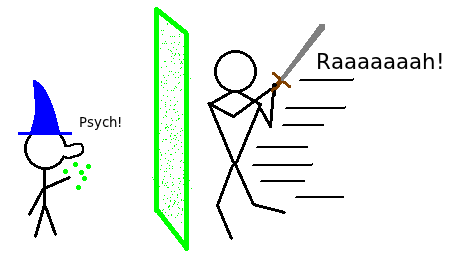
\includegraphics{Pics/WallOfForce.png}
\end{figure*}

\paragraph{Augment:} You can augment this spell in one or both of the following ways:
\begin{enumerate}
 \item For every additional spell point you spend, you get an additional 10-ft. square of wall.
 \item If you spend four additional spell points, the wall as a whole does not need to be flat, although each individual 10' section still has to be.
\end{enumerate}
\subsubsection{Wall of Ice}
\label{Spell:WallOfIce}
Evocation [Cold]
\\ \textbf{Level:} Sor/Wiz 4
\\ \textbf{Components:} V, S
\\ \textbf{Casting Time:} 1 standard action
\\ \textbf{Range:} Medium (100 ft. + 10 ft./level)
\\ \textbf{Effect:} Ice wall whose area consists of up to seven 5' squares (S)
\\ \textbf{Duration:} 1 min./level
\\ \textbf{Saving Throw:} See text
\\ \textbf{Spell Resistance:} No
\\ \textbf{Spell Points:} 7

\emph{You conjure a solid block of ice.}

This spell creates a wall of ice that merges into adjoining surfaces. 
A wall of ice is 1 inch thick per caster level and composed of up to seven 5-foot squares, 
which must join one another. 
You can double the wall's area by halving its thickness. 
The wall cannot be conjured so that it occupies the same space as a creature or another object.

You can create a wall of ice in almost any shape you desire. 
The wall created need not be vertical, nor rest upon any firm foundation; however, 
it must merge with and be solidly supported by existing stone. 
It can be used to bridge a chasm, for instance, or as a ramp. 
For this use, if the span is more than 20 feet, the wall must be arched and buttressed. 
This requirement reduces the spell's area by half. 
The wall can be crudely shaped to allow crenellations, 
battlements, and so forth by likewise reducing the area.

Walking along the vertical surface of a wall of ice requires a DC 10 balance check.
Climbing up a wall of ice follows normal rules for climbing, with a +5 modifier
to the DC for the surface being slippery.

Like any other solid wall, this one can be destroyed by a disintegrate spell or by normal means such as breaking and chipping. 
Each 5-foot square of wall has 3 hit points per inch of thickness. Its hardness is 0.
Creatures can hit the wall automatically. 
A section of wall whose hit points drop to 0 is breached. 
If a creature tries to break through the wall with raw strength rather than attacks, 
the DC for the Strength check is 22.

It is possible, but difficult, to trap mobile opponents within or under a wall of ice, 
provided the wall is shaped so it can hold the creatures. 
Creatures can avoid entrapment with successful Reflex saves.

The wall is crystal clear, and does not block line of sight (although
spot checks taken through the wall take a -2 penalty).
Noticing the wall is a DC 0 spot check.
The wall does block line of effect.

\paragraph{Augment:} For every additional spell point you spend, you get an additional 5' square of wall you can place, 
and the strength check DC required to burst through it increases by 1.
\subsubsection{Wall of Iron}
\label{Spell:WallOfIron}
Conjuration (Creation)
\\ \textbf{Level:} Conjurer 6
\\ \textbf{Components:} V, S
\\ \textbf{Casting Time:} 1 standard action
\\ \textbf{Range:} Medium (100 ft. + 10 ft./level)
\\ \textbf{Effect:} Iron wall whose area is up to eleven 5-ft. squares; see text
\\ \textbf{Duration:} 1 hour/level
\\ \textbf{Saving Throw:} None
\\ \textbf{Spell Resistance:} No
\\ \textbf{Spell Points:} 11

\emph{''Doesn't last long enough to be sold, I'm afraid.``}

You cause a flat, vertical iron wall to spring into being. 
The wall inserts itself into any surrounding nonliving material if its area is sufficient to do so,
keeping it in place. 
The wall cannot be conjured so that it occupies the same space as a creature or another object. 
It must always be a flat plane, though you can shape its edges to fit the available space.

A wall of iron is 1 inch thick per four caster levels. %You can double the wall's area by halving its thickness. 
Each 5-foot square of the wall has 30 hit points per inch of thickness and hardness 10. 
A section of wall whose hit points drop to 0 is breached. 
If a creature tries to break through the wall with a single attack, the DC for the Strength check is 25 + 2 per inch of thickness.

If you desire, the wall can be created (nearly) vertically resting on a flat surface but not attached to the surface, 
so that it tips over and crushes creatures caught in the area (the wall must have sufficient space to tip over). 
A wall so conjured crashes to the ground after one round (on your initiative in the next round) if left to fall on its own.
Any large or smaller creature caught under the wall (naturally, the effective area becomes equal to the size of the wall)
when it touches down takes 11d6 points of damage and is Immobilized until he makes a successful DC 40 strength or escape artist check 
(or the wall is dispelled or expires).
The presence of any huge or larger creature in the affected area causes the wall to automatically stabilize, negating the effect for all creatures.

In the round the wall spends falling, a creature adjacent to one of the squares in which the wall was conjured can use a move action 
to reverse the direction of the fall with a DC 30 strength check, 
or stabilize the wall in the position in which it was originally conjured with a DC 30 strength check and a DC 20 Balance check.

\paragraph{Augment:} For every additional spell point you spend, you can create a wall with an area of one additional 5' square. This increases the
damage dealt to crushed creatures by 1d6, and increases the DC of the strength or escape artist checks to escape after being pinned by the wall by 1, 
as well as the strength DCs to affect the fall of the wall.
\subsubsection{Wall of Stone}
\label{Spell:WallOfStone}
Conjuration (Creation) [Earth]
\\ \textbf{Level:} Earth 5, Sor/Wiz 5
\\ \textbf{Effect:} Stone wall whose area consists of up to nine 5' squares (S)
\\ \textbf{Duration:} Instantaneous
\\ \textbf{Spell Points:} 9

\textbf{A thick rock outcropping appears.}

This spell works like \nameref{Spell:WallOfIce}, except as noted here.

\begin{list}{\labelitemi}{\leftmargin=1em}
 \item A wall of stone is 1 inch thick per two caster levels.
 \item No balance checks are required to remain stable on a stone wall, and climbers are not at a particular disadvantage.
 \item Each 5-foot square of stone wall has 15 hit points per inch of thickness. Its hardness is 8.
The DC for a Strength check to break through it is 30.
 \item Stone walls are opaque, and block line of sight.
\end{list}

\paragraph{Augment:} For every additional spell point you spend, you get an additional 5' square of wall you can place, 
and the strength check DC required to burst through it increases by 1.
\subsubsection{Wall of Thorns}
\label{Spell:WallOfThorns}
Conjuration (Creation)
\\ \textbf{Level:} Plant 5, Ranger 5
\\ \textbf{Components:} V, S
\\ \textbf{Casting Time:} 1 standard action
\\ \textbf{Range:} Medium (100 ft. + 10 ft./level)
\\ \textbf{Effect:} Wall of thorny brush, up to nine 10-ft. cubes(S)
\\ \textbf{Duration:} 10 min./level (D)
\\ \textbf{Saving Throw:} None
\\ \textbf{Spell Resistance:} No
\\ \textbf{Spell Points:} 9

\emph{You create a barrier of very tough, pliable, tangled brush bearing needle-sharp thorns as long as a human's finger.}

Any creature forced into or attempting to move through a wall of thorns takes slashing damage per round of movement equal to 25 minus the creature's AC (minimum 0). Dexterity and dodge bonuses to AC do not count for this calculation.

You can make the wall as thin as 5 feet thick, which allows you to shape the wall as a number of 10-by-10-by-5-foot blocks equal to twice your caster level. This has no effect on the damage dealt by the thorns, but any creature attempting to break through takes that much less time to force its way through the barrier.

Creatures can force their way slowly through the wall by making a Strength check as a full-round action. For every 5 points by which the check exceeds 20, a creature moves 5 feet (up to a maximum distance equal to its normal land speed). Of course, moving or attempting to move through the thorns incurs damage as described above. A creature trapped in the thorns can choose to remain motionless in order to avoid taking any more damage.

Any creature within the area of the spell when it is cast takes damage as if it had moved into the wall and is caught inside. In order to escape, it must attempt to push its way free, or it can wait until the spell ends. Creatures with the ability to pass through magically overgrown areas unhindered can pass through a wall of thorns at normal speed without taking damage.

A wall of thorns can be breached by slow work with edged weapons. Chopping away at the wall creates a safe passage 1 foot deep for every 10 minutes of work. Fire burns a 10' cube of it away in 10 minutes.

Despite its appearance, a wall of thorns is not actually a living plant, and thus is unaffected by spells that affect plants.

\paragraph{Augment:} For every additional spell point you spend, you can create a wall with an area of one additional 5' square, and the damage dealt by the spell increases by 1.
\subsubsection{Warrior's Impetus}
\label{Spell:WarriorsImpetus}
Transmutation
\\ \textbf{Level:} War 5
\\ \textbf{Components:} V, S
\\ \textbf{Casting Time:} 1 standard action
\\ \textbf{Range:} Close (25 ft. + 5 ft./2 levels)
\\ \textbf{Target:} One creature
\\ \textbf{Duration:} 1 round/level
\\ \textbf{Saving Throw:} None
\\ \textbf{Spell Resistance:} Yes
\\ \textbf{Spell Points:} 9

\emph{You imbue your allies with a portion of the speed and power of all warriors who have ever followed your cause.}

When making a full attack action, a targeted creature may make one extra attack with any weapon he is holding. 
The attack is made using the creature's full base attack bonus, plus any modifiers appropriate to the situation. 
(This effect is not cumulative with similar effects, such as that provided by a \nameref{Spell:Haste}, nor does it actually grant an extra action, so you can't use it to cast a second spell or otherwise take an extra action in the round.)

The targets also gain a +3 morale bonus on attack rolls and damage rolls. (This bonus on attack rolls stacks with the untyped bonus provided by \nameref{Spell:Haste}.)
\paragraph{Augment:} For every additional spell point you spend, this spell can affect an additional creature.
\subsubsection{Water Walk}
\label{Spell:WaterWalk}
Transmutation [Water]
\\ \textbf{Level:} Ranger 3, Water 3
\\ \textbf{Components:} V, S
\\ \textbf{Casting Time:} 1 standard action
\\ \textbf{Range:} Touch
\\ \textbf{Targets:} Up to five touched creatures
\\ \textbf{Duration:} 10 min./level (D)
\\ \textbf{Saving Throw:} Will negates (harmless)
\\ \textbf{Spell Resistance:} Yes (harmless)
\\ \textbf{Spell Points:} 5

\emph{''For a spell no more complicated than this, it sure freaks out the villagers.``}

The transmuted creatures can tread on any liquid as if it were firm ground. 
Mud, oil, snow, quicksand, running water, ice, and even lava can be traversed easily, since the subjects' feet hover an inch or two above the surface. 
(Creatures crossing molten lava still take damage from the heat because they are near it.) 
The subjects can walk, run, charge, or otherwise move across the surface as if it were normal ground.

If the spell is cast underwater (or while the subjects are partially or wholly submerged in whatever liquid they are in), the subjects are borne toward the surface at 60 feet per round until they can stand on it.

\paragraph{Augment:} For every additional spell point you spend, you can target an additional creature when casting this spell.
\subsubsection{Waves of Fatigue}
\label{Spell:WavesOfFatigue}
Necromancy
\\ \textbf{Level:} Sor/Wiz 5
\\ \textbf{Components:} V, S
\\ \textbf{Casting Time:} 1 standard action
\\ \textbf{Range:} 30 ft.
\\ \textbf{Area:} Cone-shaped burst
\\ \textbf{Duration:} Instantaneous
\\ \textbf{Saving Throw:} No
\\ \textbf{Spell Resistance:} Yes
\\ \textbf{Spell Points:} 9

\emph{Waves of negative energy radiate outwards from you.}

All living creatures in the spell's area are rendered \emph{fatigued}. This spell has no effect on a creature that is already \emph{fatigued}.

\paragraph{Augment:} If you spend an additional 4 spell points, this spell renders its victims \emph{exhausted} rather than \emph{fatigued}.
\subsubsection{Web}
\label{Spell:Web}
Conjuration (Creation)
\\ \textbf{Level:} Sor/Wiz 2, Vermin 2
\\ \textbf{Components:} V, S
\\ \textbf{Casting Time:} 1 standard action
\\ \textbf{Range:} Medium (100 ft. + 10 ft./level)
\\ \textbf{Effect:} Web between two anchors
\\ \textbf{Duration:} 10 min./level (D)
\\ \textbf{Saving Throw:} Reflex negates; see text
\\ \textbf{Spell Resistance:} No
\\ \textbf{Spell Points:} 3

\emph{You create a many-layered mass of strong, sticky strands, similar to spider webs but far larger and tougher.}

The web you create must be anchored to two or more solid and diametrically opposed points or else it collapses upon itself and disappears. 
The two anchor points must be within 40' of each other, making that the maximum length of the web. The web extends 15' down from the anchoring points. 

To determine the web's ground area, draw a line between the two anchors. The web occupies all squares crossed by that line.

%Creatures caught within a web become Immobilized among the gluey fibers. 
%Attacking a creature in a web won't cause you to become Immobilized.
Anyone in the effect's area when the spell is cast must make a Reflex save. 
If this save succeeds, the creature escapes, and is shunted to the nearest empty space 
(if multiple squares are equally valid, the creature chooses which square it ends up in). 
%This movement counts against the creature's movement on its next turn (or its 5' step), possibly restricting its actions.

If the save fails, the creature is \emph{immobilized} and can't move from its space,  
but can break loose by spending a full round action and making a DC 20 Strength check or a DC 25 Escape Artist check 
(if the creature attempting to escape succeeds by 4 or more, the square of webs the creature occupied is destroyed).
Once loose, the creature ends up in the nearest empty square, as if it had succeeded on the initial reflex save.

If you have web between you and an opponent, it provides cover.

The strands of a web spell are extremely flammable. 
A magic flaming sword can slash them away as easily as a hand brushes away cobwebs, automatically destroying a 
5'x5' square of the webs with a single attack.
Any fire can set the webs alight and burn away a square in 1 round. 
All creatures Immobilized within a square of flaming webs take 2d4 points of fire damage from the flames.

Each square of webs has 20 hit points and hardness 5 (slashing weapons ignore this hardness).
Each square can be burst with a DC 24 Strength check.

%Web can be made permanent with a permanency spell. A permanent web that is damaged (but not destroyed) regrows in 10 minutes.

%\paragraph{Augment:} For every 2 additional spell points you spend, this spell's save DC increases by 1.

\subsubsection{Web Strand}
\label{Spell:WebStrand}
Conjuration (Creation)
\\ \textbf{Level:} Vermin 1
\\ \textbf{Components:} V, S
\\ \textbf{Casting Time:} 1 standard action
\\ \textbf{Range:} Close (25 ft. + 5 ft./2 levels)
\\ \textbf{Target:} One Medium or smaller creature
\\ \textbf{Duration:} 5 rounds
\\ \textbf{Saving Throw:} None
\\ \textbf{Spell Resistance:} No
\\ \textbf{Spell Points:} 1

\emph{You conjure forth a sticky strand of webbing, like that of an oversized spider, and hurl it at your enemy.}

You throw the strand of webbing as a ranged touch attack at any creature in range. 
On a successful hit, the subject is covered in goo and becomes \emph{entangled}. 
The goo evaporates at the end of the spell's duration.

\paragraph{Augment:} For every 2 additional spell points you spend, this spell can affect a target one size category larger.

\subsubsection{Whirlwind}
\label{Spell:Whirlwind}
Evocation [Air]
\\ \textbf{Level:} Air 8
\\ \textbf{Components:} V, S
\\ \textbf{Casting Time:} 1 standard action
\\ \textbf{Range:} Long (400 ft. + 40 ft./level)
\\ \textbf{Effect:} Cyclone 10 ft. wide at base, 30 ft. wide at top, and 30 ft. tall
\\ \textbf{Duration:} 1 round/level (D)
\\ \textbf{Saving Throw:} Reflex negates; see text
\\ \textbf{Spell Resistance:} No
\\ \textbf{Spell Points:} 15

\emph{This spell creates a powerful cyclone of raging wind.} 

The cyclone can move through the air, along the ground, or over water at a speed of 60 feet per round. 

You can concentrate on controlling the cyclone's every movement or specify a simple program. 
Directing the cyclone's movement or changing its programmed movement is a standard action for you. 
The cyclone always moves during your turn. 
If the cyclone exceeds the spell's range, it moves in a random, uncontrolled fashion for 1d3 rounds and then dissipates. (You can't regain control of the cyclone, even if comes back within range.)

Any large or smaller creature that comes in contact with the spell effect must succeed on a Reflex save or take 7d6 points of damage. 
Regardless of the outcome of the first save, a medium or smaller creature must succeed on a second one or be picked up bodily by the cyclone and held suspended in its powerful winds, taking 2d8 points of damage each round on your turn with no save allowed. This is considered continuous damage for purposes of determining whether or not concentration checks are needed to use abilities. Escaping the cyclone via mundane means (even flight) requires a DC 40 escape artist check. A creature who escapes is \emph{blown away} in a direction of its choosing, away from the cyclone.

You may direct the cyclone to eject any carried creatures whenever you wish. When so released, they are \emph{blown away} in a direction of your choosing, away from the cyclone.

\paragraph{Augment:} For every additional spell point you spend, the spell's initial damage increases by one die (d6), and the escape artist DC to get out of the cyclone increases by 1.
\subsubsection{Widowmaker Blade}
\label{Spell:WidowmakerBlade}
Necromancy [Death, Evil]
\\ \textbf{Level:} Blackguard 5
\\ \textbf{Components:} V, S
\\ \textbf{Casting Time:} 1 standard action
\\ \textbf{Range:} Touch
\\ \textbf{Targets:} One melee weapon
\\ \textbf{Duration:} 1 round/level
\\ \textbf{Saving Throw:} Will negates (harmless, object); see text
\\ \textbf{Spell Resistance:} Yes (harmless, object)
\\ \textbf{Spell Points:} 9

\emph{The weapon you touch becomes an instrument to cull the weak from the battlefield.} 

Any living creature with HD equal to or less than 7 must succeed on a Fortitude save or die if struck in combat with this weapon. 
Spell resistance does not apply against the death effect.

In addition, the wielder gains the benefit of the Cleave feat as long as he holds the weapon. If he already has the Cleave feat, he gains the Great Cleave feat instead. If he already has the Great Cleave feat, he receives no additional benefit.

\paragraph{Augment:} For every additional spell point you spend, the weapon can affect a creature with 1 more HD.

\subsubsection{Wind Wall}
\label{Spell:WindWall}
Evocation [Air]
\\ \textbf{Level:} Air 3, Ranger 2, Sor/Wiz 3
\\ \textbf{Components:} V, S
\\ \textbf{Casting Time:} 1 standard action
\\ \textbf{Range:} Medium (100 ft. + 10 ft./level)
\\ \textbf{Effect:} Wall up to 10 ft./level long and 5 ft./level high (S)
\\ \textbf{Duration:} 1 round/level
\\ \textbf{Saving Throw:} Special; see text
\\ \textbf{Spell Resistance:} Yes
\\ \textbf{Spell Points:} Air 5, Ranger 3, Sor/Wiz 3

\emph{You create an area infested with gusts of powerful wind directed downwards, hindering the advance of creatures and making ranged attacks very difficult.}

The wall you create is 5 feet thick, and not directly visible. However, dirt and loose
debris in its area is blown around, often giving it away. While the wall must be vertical, 
you can shape it in any continuous path along the ground that you like. 
It is possible to create cylindrical or square wind walls to enclose specific points.

Any physical missiles (arrows, crossbow bolts, javelins, magically propelled stones, and so on) whose line of effect passes through the
wind wall have a 50\% miss chance.

Passing through the wall is difficult.
Every time a creature enters a space the wall occupies, it must make a strength check or be knocked down.
The DC for the strength check is equal to the spell's save DC. 
For every size category the creature is above medium, it gains a +4 bonus on the strength check.
For every size category the creature is below medium, it suffers a -4 penalty on the strength check.
Flying creatures or those for some other reason not in contact with the ground (such as due to jumping) 
suffer a -8 penalty on the strength check in addition to the modifiers for size, above.

If the creature succeeds on the strength check, it manages to push through the wall unhindered.
If the creature fails, it is knocked prone in the space it was trying to enter, and takes 1d6 points of nonlethal damage.
Flying creatures are instantly knocked to the ground, and take damage as if they had fallen from the distance they were
flying (\nameref{Spell:ControlFall} does not prevent this).

Standing up while in the wind wall's area is difficult, and requires a successful strength check (which uses the same modifiers
and DCs as those for entering a square filled by the wall).

It is impossible to charge through a wind wall.
Gases, most gaseous breath weapons, and creatures in \nameref{Spell:GaseousForm} cannot pass through the wall.
It is no barrier to incorporeal creatures and air elementals.

The force of the gust automatically extinguishes candles, torches, and similar unprotected flames in its area. 
It causes protected flames, such as those of lanterns, to dance wildly and has a 50\% chance to extinguish those lights.

% \paragraph{Augment:} For every 2 additional spell points you spend, this spell's save DC increases by 1, and the miss chance
% suffered by missiles passing through the wall is increased by 10\% (to a maximum of 100\%).
\paragraph{Augment:} For every additional spell point you spend, the miss chance suffered by missiles passing though the wall
is increased by 5\% (to a maximum of 100\%).
\subsubsection{Wish}
\label{Spell:Wish}
Evocation
\\ \textbf{Level:} Sor/Wiz 9
\\ \textbf{Components:} V
\\ \textbf{Casting Time:} 1 standard action
\\ \textbf{Range:} See text
\\ \textbf{Target, Effect, or Area:} See text
\\ \textbf{Duration:} See text
\\ \textbf{Saving Throw:} See text
\\ \textbf{Spell Resistance:} Yes
\\ \textbf{Spell Points:} 17, XP

\emph{Wish is the mightiest spell a spellcaster can cast. By simply speaking aloud, you can alter reality to better suit you.
It is a tool fit for a god.}

\begin{figure*}
  \caption{Sorcerer receives the world's largest cockerel as a result of his Wish.}
  \centering
    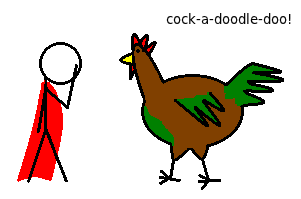
\includegraphics{Pics/Wish.png}
\end{figure*}

A Wish can produce any one of the following effects. 
These effects are easily within the power of the Wish, unintended consequences are next to impossible.
\begin{list}{\labelitemi}{\leftmargin=1em}
  \item Duplicate any wizard spell of 8th level or lower, other than a spell restricted to specialists of schools other than your own.
  \item Duplicate any wizard spell of 7th level or lower, even if it is a spell restricted to specialists of schools other than your own.
  \item Duplicate any other spell of 6th level or lower.
  \item Undo the harmful effects of many other spells, such as \nameref{Spell:GeasQuest} or an augmented \nameref{Spell:Confusion}.
  \item Create a nonmagical item of up to 25,000 gp in value.
  \item Create a magic item, or add to the powers of an existing magic item (see XP cost below).
  %\item Grant a creature a +1 inherent bonus to an ability score. Two to five Wish spells cast in succession (which need not be an immediate succession) can grant a creature a +2 to +5 inherent bonus to an ability score (two Wishes for a +2 inherent bonus, three for a +3 inherent bonus, and so on).
  \item Grant a creature a +1 inherent bonus to an ability score, or increase an existing inherent bonus to an ability score by one.
  Inherent bonuses are instantaneous, so they cannot be dispelled. An inherent bonus may not exceed +5 for a single ability score.
  %An inherent bonus may not exceed +5 for a single ability score, and inherent bonuses to a particular ability score do not stack, so only the best one applies.
  \item Remove injuries and afflictions. A single Wish can aid one creature per caster level, and all subjects are cured of the same kind of affliction. 
  For example, you could heal all the damage you and your companions have taken, or remove all poison effects from everyone in the party, but not do both with the same Wish. 
  A Wish can never restore the experience point loss from casting a spell or the level or Constitution loss from being raised from the dead.
  \item Revive the dead. A Wish can bring a dead creature back to life by duplicating a resurrection spell. .
  A Wish can revive a dead creature whose body has been destroyed, but the task takes two Wishes, one to recreate the body and another to infuse the body with life again. 
  A Wish cannot prevent a character who was brought back to life from losing an experience level.
  \item Transport travelers. A Wish can lift one creature per caster level from anywhere on any plane and place those creatures anywhere else on any plane regardless of local conditions, 
  excepting the direct intervention of a deity. 
  An unwilling target gets a Will save to negate the effect, and spell resistance (if any) applies.
  \item Undo misfortune. A Wish can undo a single recent event. 
  The Wish forces a reroll of any roll made within the last round (including your last turn). 
  Reality reshapes itself to accommodate the new result. 
  For example, a Wish could undo an opponent's successful save, a foe's successful critical hit (either the attack roll or the critical roll), 
  a friend's failed save, and so on. The reroll, however, may be as bad as or worse than the original roll. 
  An unwilling target gets a Will save to negate the effect, and spell resistance (if any) applies.
  \item Produce any other effect whose power level is in line with the above effects
\end{list}
You may try to use a Wish to produce greater effects than these, but doing so is dangerous. 
(The Wish may pervert your intent into a literal but undesirable fulfillment or only a partial fulfillment.)
You can describe virtually any effect, but you must do so in 10 words or less.

Duplicated spells allow saves and spell resistance as normal (but save DCs are for the number of spell points spent on the Wish).

\emph{Experience Cost:} The minimum XP cost for casting Wish is 5,000 XP. 
When a Wish duplicates a spell that has an XP cost, you must pay 5,000 XP or that cost, whichever is more. 
When a Wish creates or improves a magic item, you must pay twice the normal XP cost for crafting or improving the item, plus an additional 5,000 XP. 

\subsubsection[Limited Wish]{Wish, Limited}
\label{Spell:LimitedWish}
Evocation
\\ \textbf{Level:} Magic 7, Sor/Wiz 7
\\ \textbf{Components:} V
\\ \textbf{Casting Time:} 1 standard action
\\ \textbf{Range:} See text
\\ \textbf{Target, Effect, or Area:} See text
\\ \textbf{Duration:} See text
\\ \textbf{Saving Throw:} See text
\\ \textbf{Spell Resistance:} Yes
\\ \textbf{Spell Points:} 13, XP

\emph{You learn to create nearly any type of effect.}

A Limited Wish can do any of the following:
\begin{list}{\labelitemi}{\leftmargin=1em}
\item Duplicate any wizard spell of 6th level or lower, other than a spell restricted to specialists of schools other than your own.
\item Duplicate any wizard spell of 5th level or lower,  even if it is a spell restricted to specialists of schools other than your own.
\item Duplicate any other spell of 4th level or lower.
\item Undo the harmful effects of many spells, such as \nameref{Spell:GeasQuest} or an augmented \nameref{Spell:Confusion}.
\item Produce any other effect whose power level is in line with the above effects, 
such as a single creature automatically hitting on its next attack or taking a -7 penalty on its next saving throw.
\end{list}
A duplicated spell allows saving throws and spell resistance as normal (but save DCs are for the number of spell points spent on the Wish).

When Limited Wish duplicates a spell that has an XP cost, you must pay that cost or 300 XP, whichever is more. 

\emph{Experience cost:} 300 XP or more (see above).
\subsubsection{Woodbolt}
\label{Spell:Woodbolt}
Conjuration (Creation)
\\ \textbf{Level:} Plant 1
\\ \textbf{Components:} V, S
\\ \textbf{Casting Time:} 1 standard action
\\ \textbf{Range:} Close (25 ft. + 5 ft./2 levels)
\\ \textbf{Effect:} Ray
\\ \textbf{Duration:} Instantaneous
\\ \textbf{Saving Throw:} None
\\ \textbf{Spell Resistance:} None
\\ \textbf{Spell Points:} 1

\emph{You create a spearlike branch that hurls itself at your enemies.}

You create a wooden bolt shoots forth from your outstretched arm and strikes a target within range, dealing 1d6 points of damage.
You must succeed on a ranged attack (not a ranged touch attack) with the bolt for it to deal damage.

\paragraph{Augment:} For every additional spell point you spend, this spell's damage increases by one die (d6).
\subsubsection{Wombat's Boost}
\label{Spell:WombatsBoost}
Transmutation
\\ \textbf{Level:} Assassin 2, Blackguard 2, Cleric 2, Paladin 2, Sor/Wiz 2
\\ \textbf{Components:} V, S
\\ \textbf{Casting Time:} 1 standard action
\\ \textbf{Range:} Touch
\\ \textbf{Target:} Creature touched; see text
\\ \textbf{Duration:} 1 min./level
\\ \textbf{Saving Throw:} Will negates (harmless)
\\ \textbf{Spell Resistance:} Yes
\\ \textbf{Spell Points:} 3

\emph{The affected creature is infused with power.} 

The creature is granted a +4 enhancement bonus to a single ability score of the caster's choice, chosen at the time of casting. 

The individual functions of this spell are often named after animals that embody the ability in question in the
eyes of some scolars. They are \emph{Bull's Strength}, \emph{Cat's Grace} (Dexterity),
\emph{Bear's Endurance} (Constitution), \emph{Owl's Wisdom}, 
\emph{Fox's Cunning} (Intelligence), and \emph{Eagle's Splendor} (Charisma).

Unlike \nameref{Spell:AlterSelf}, the enhancement to your ability does not result in a physical change -
the improvement is due to a direct magical infusion.

\begin{figure*}
  \caption{Wizard casts Bull's Strength on himself to know how it is to be as strong as the Fighter.}
  \centering
    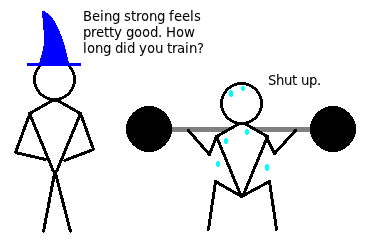
\includegraphics{Pics/Wombat.png}
\end{figure*}

\paragraph{Augment:} You can Augment this spell in one or both of the following ways:
\begin{enumerate}
 \item If you spend two additional spell points, the spell's range increases to Close.
 \item For every two additional spell points you spend, the spell can affect an additional target.
\end{enumerate}
\subsubsection{Word of God}
\label{Spell:WordOfGod}
Evocation [Sonic, see text]
\\ \textbf{Level:} Blackguard 6, Chaos 7, Evil 7, Good 7, Law 7, Paladin 6
\\ \textbf{Components:} V
\\ \textbf{Casting Time:} 1 standard action
\\ \textbf{Range:} 40 ft.
\\ \textbf{Area:} Creatures in a 40-ft.-radius spread centered on you
\\ \textbf{Duration:} Instantaneous; see text
\\ \textbf{Saving Throw:} None or Will negates; see text
\\ \textbf{Spell Resistance:} Yes
\\ \textbf{Spell Points:} Chaos 13, Evil 13, Good 13, Law 13, Paladin 11

\emph{A single bass note of incredible power suffuses the area.}

When casting this spell, choose an alignment. The spell gains that alignment as a descriptor.

Any creature not of your selected alignment within the spell's area suffers the ill effects
described on the \nameref{tab:WordOfGod} table. This includes you, if you are not of the selected alignment.
\begin{table*}
\label{tab:WordOfGod}
\caption{Word of God}
\makebox[\textwidth]{
\begin{tabular}{|l|cccc|l|}
\hline
&\multicolumn{4}{c|}{Alignment selected}&\\
$\leq$HD&Chaotic&Evil&Good&Law&Duration\\
&(Word of Chaos)&(Blasphemy)&(Holy Word)&(Dictum)&\\
\hline
14&Unaffected&Unaffected&Unaffected&Unaffected&N/A\\
13&Deafened&Deafened&Deafened&Deafened&Permanent\\
9-12&Stunned (1d3)&Blinded (2d4)&Nauseated (1d4)&Dazed (1d3)&Rounds, see entry\\
4-8&Paralyzed&Paralyzed&Paralyzed&Paralyzed&1d10 minutes\\
3&Killed&Killed&Killed&Killed&Instantaneous\\
\hline
\end{tabular}}
\end{table*}

\begin{figure*}
  \caption{Cleric uses Word of God effectively.}
  \centering
    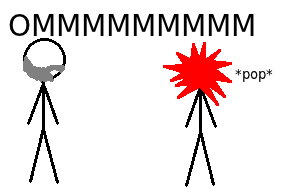
\includegraphics{Pics/WordOfGod.png}
\end{figure*}

The number of HD indicated on the table refers to the maximum number of HD a creature may have in order to be subjected to the corresponding effect.
The effects are cumulative and concurrent.
For example, an evil creature with 10 HD caught in a good-aligned Word of God is \emph{nauseated} and \emph{deafened}.

\paragraph{Augment:} For every additional spell point you spend, the number of HD indicated in each row of the first column of the \nameref{tab:WordOfGod} table increases by 1.
\subsubsection{Word of Recall}
\label{Spell:WordOfRecall}
Conjuration (Teleportation)
\\ \textbf{Level:} Protection 6, Travel 6
\\ \textbf{Components:} V
\\ \textbf{Casting Time:} 1 standard action
\\ \textbf{Range:} Unlimited
\\ \textbf{Target:} You and touched objects or other willing creatures
\\ \textbf{Duration:} Instantaneous
\\ \textbf{Saving Throw:} None or Will negates (harmless, object)
\\ \textbf{Spell Resistance:} No or Yes (harmless, object)
\\ \textbf{Spell Points:} 11

\emph{''HOME! ``}

Word of recall teleports you instantly back to your sanctuary when cast. 

You must designate this sanctuary before using the spell.
Doing so involves a simple ritual performed at the site, taking one hour. 
The sanctuary must be a place very familiar to you. 
The actual point of arrival is a designated area no larger than 10 feet by 10 feet.
You can choose a new sanctuary by re-doing the ritual at another site.

You can be transported any distance within a plane but cannot travel between planes. 
You can transport, in addition to yourself, any objects you carry, as long as their weight doesn't exceed your maximum load. 
You may also bring one additional willing creature (carrying gear or objects up to its maximum load) per three caster levels. 
All creatures to be transported must be in contact with one another, and at least one of those creatures must be in contact with you. Exceeding this limit causes the spell to fail.

An unwilling creature can't be teleported by word of recall. Likewise, a creature's Will save (or spell resistance) prevents items in its possession from being teleported. Unattended, nonmagical objects receive no saving throw.

\paragraph{Augment:} If you spend 4 additional spell points, the spell can teleport you towards a sanctuary on another plane.
\subsection{'X' Spells}
\subsubsection{X-ray Vision}
\label{Spell:XRayVision}
Divination
\\ \textbf{Level:} Sor/Wiz 5
\\ \textbf{Components:} V, S
\\ \textbf{Casting Time:}  1 standard action
\\ \textbf{Range:} Personal
\\ \textbf{Target:} You
\\ \textbf{Duration:} 1 min./level
\\ \textbf{Spell Points:} 9

\emph{''The toughest part is to remember to open your door.``}

You gain the ability to see into and through solid matter.

The range of the X-ray vision is 20'. Within this range, you see as if in normal light even if there is no illumination (magical darkness is ignored as well). X-ray vision can penetrate 1 foot of stone, 1 inch of metal, or up to 3 feet of wood or dirt. A thin sheet of lead blocks the vision.
X-ray vision is black and white only but otherwise functions like normal sight.

Note that although X-ray vision may pierce certain forms of concealment, it does not grant line of effect.

In addition, you gain a +4 bonus on Heal checks made to re-set broken bones.

\paragraph{Augment:} You can augment this spell in one or both of the following ways:
\begin{enumerate}
 \item For every 2 additional spell points you spend, the radius of your X-ray vision increases by 5 feet.
 \item If you spend 4 additional spell points, stone, metal, wood and dirt do not block the X-ray vision. 
\end{enumerate}

\subsection{'Z' Spells}
\subsubsection{Zone of Truth}
\label{Spell:ZoneOfTruth}
Abjuration
% \\ \textbf{Level:} Law 2, Paladin 2
% \\ \textbf{Components:} V, S
% \\ \textbf{Casting Time:} 1 standard action
% \\ \textbf{Range:} Close (25 ft. + 5 ft./2 levels)
% \\ \textbf{Area:} 10-ft.-radius emanation centered on a point in space
% \\ \textbf{Duration:} 10 min./level (D)
% \\ \textbf{Saving Throw:} None
% \\ \textbf{Spell Resistance:} No
% \\ \textbf{Spell Points:} 3
\Level{Law 2, Paladin 2}
\Components{V, S}
\CastingTime{1 standard action}
\Range{\CloseRange}
\Area{10-ft.-radius emanation centered on a point in space}
\Duration{\TenMinLevelDuration{\DismissibleSpell}}
\SavingThrow{None}
\SRno
\SP{3}

\emph{Your tongue physically resists when you try speaking anything but the honest truth.}

All creatures within the spell's area take a penalty on Bluff checks equal to 10 + your caster level.

\paragraph{Augment:} If you spend 4 additional spell points, the spell's duration changes to 1 day.

\newpage
\subsection{Where's my favorite spell?}
\label{sec:MissingSpells}
This conversion does not contain all the spells in the \href{http://www.wizards.com/default.asp?x=d20/article/srd35}{d20 srd}.
Some were merged into others, some were merely renamed, but some truly aren't here. 
The most common reason for a spell not being included was it being too limited in scope to justify being a spell of its own under the revised system.
This is a list of all SRD spells that do not have a converted spell with the same name.
Note that some spells might have changed levels.
{\small
\begin{list}{\labelitemi}{\leftmargin=1em}
 \item Acid Fog: Merged into Deadly Fog.
 \item Acid Splash: See the Cantrips class feature.
 \item Analyze Dweomer: Merged into Identify.
 \item Animal Growth: Merged into Alter Animal's Size.
 \item Animal Shapes: Removed. Replace with Form of the Predator for item creation and other purposes.
 \item Animal Trance: Removed. Replace with Pattern for item creation and other purposes.
 \item Animate Rope: Removed. Replace with Animate objects for item creation and other purposes.
 \item Antipathy: Merged into Telepathic Beacon
 \item Antiplant Shell: Removed. Replace with Antilife Shell for item creation and other purposes.
 \item Arcane Lock: Merged into Open/Close.
 \item Arcane Mark: See the Cantrips class feature.
 \item Arcane Sight, Greater: Merged into Detect Magic.
 \item Arcane Sight: Merged into Detect Magic.
 \item Banishment: Merged into Dismissal.
 \item Bear's Endurance, Bull's Strength, Cat's Grace, Eagle's Splendor, Fox's Cunning and Owl's Wisdom, Mass: Merged into Wombat's Boost.
 \item Bear's Endurance, Bull's Strength, Cat's Grace, Eagle's Splendor, Fox's Cunning and Owl's Wisdom: Merged into Wombat's Boost.
 \item Blasphemy/Dictum/Holy Word/Word of Chaos: Merged into Word of God.
 \item Break Enchantment: Merged into Remove Curse.
 \item Burning Hands: Merged into Energized Touch.
 \item Call Lightning Storm: Merged into Call Lightning.
 \item Calm Animals: Removed. Replace with Calm Emotions for item creation and other purposes.
 \item Cause Fear: Renamed Fear.
 \item Changestaff: Merged into Liveoak.
 \item Charm Animal: Isn't this what Wild Empathy is for? Removed. Replace with Charm for item creation and other purposes.
 \item Charm Monster, Mass: Merged into Charm.
 \item Charm Monster: Merged into Charm.
 \item Charm Person: Renamed Charm.
 \item Chill Touch: Merged into Energized Touch.
 \item Circle of Death: Merged into Life and Death.
 \item Clenched Fist: Pending. Can't think of more Hand spells.
 \item Clone: Merged into Gentle Repose.
 \item Cloudkill: Merged into Noxious Vapors.
 \item Command Plants: Renamed Command Nature's Allies.
 \item Continual Flame: Merged into Light.
 \item Control Plants: Renamed Control Nature's Allies.
 \item Create Greater Undead: Merged into Create Undead.
 \item Create Water: See Water domain.
 \item Crushing Hand: Pending. Can't think of more Hand spells.
 \item Cure Critical Wounds, Mass: Merged into Cure Wounds.
 \item Cure Critical Wounds: Merged into Cure Wounds.
 \item Cure Light Wounds, Mass: Merged into Cure Wounds.
 \item Cure Light Wounds: Merged into Cure Wounds.
 \item Cure Moderate Wounds, Mass: Merged into Cure Wounds.
 \item Cure Moderate Wounds: Merged into Cure Wounds.
 \item Cure Serious Wounds, Mass: Merged into Cure Wounds.
 \item Dancing Lights: See the Cantrips class feature.
 \item Daylight: Merged into Light.
 \item Daze Monster: Merged into Daze.
 \item Deathwatch: Turned into a Healing domain ability.
 \item Deep Slumber: Merged into Sleep.
 \item Delayed Blast Fireball: Changed into a Metamagic feat. Replace with fireball for item creation and other purposes.
 \item Delay Poison: Merged into Antipoison.
 \item Demand: Removed, replaced with Scrying + the Scry and Die feat. Replace with Suggestion for item creation and other purposes.
 \item Destruction: Merged into Slay Living.
 \item Detect Animals or Plants: Removed. What is this even? Replace with 4 ranks in Spot for item creation and other purposes.
 \item Detect Chaos/Evil/Good/Law: Merged into Discern Alignment.
 \item Detect Snares and Pits: Removed. Replace with Trapfinding for item creation and other purposes.
 \item Detect Thoughts: Renamed Read Thoughts.
 \item Detect Undead: Removed. Replace with Discern Alignment
 \item Diminish Plants: Merged into Plant Growth.
 \item Discern Lies: Removed due to overlap with Zone of Truth.
 \item Discern Location: Renamed Absolute Revelation, due to me thinking that ``Discern Location'' and ``Location'' are too similar.
 \item Dispel Chaos/Evil/Good/Law: Merged into Dispel Alignment
 \item Dispel Magic, Greater: Merged into Dispel Magic.
 \item Displacement: Merged into Blur.
 \item Disrupt Undead: Removed. Replace with Align Water for item creation and other purposes.
 \item Divination: Merged into Augury.
 \item Dominate Animal: Merged into Dominate.
 \item Dominate Monster: Merged into Dominate.
 \item Dominate Person: Merged into Dominate.
 \item Doom: Merged into Fear.
 \item Energy Drain: Merged into Enervation.
 \item Enlarge Person, Mass: Merged into Alter Size.
 \item Enlarge Person: Merged into Alter Size.
 \item Enthrall: Removed. Replace with Charm for item creation and other purposes.
 \item Erase: Removed. Replace with the Cantrip class feature for item creation and other purposes.
 \item Etherealness: Merged into Ethereal Jaunt.
 \item Fabricate: Merged into Mold Material.
 \item Feather Fall: Merged into Control Fall.
 \item Find the Path: Removed, pending inspiration. Replace with Legend Lore for purposes of item creation.
 \item Find Traps: Renamed Trap Intuition.
 \item Fire Shield: Renamed Aura of Fire.
 \item Fire Trap: Replaced with Explosive Runes.
 \item Flame Arrow: Renamed Energy Arrow.
 \item Flare: Merged into Light.
 \item Flesh to Stone: Merged into Transmute Flesh and Stone
 \item Fog Cloud: Merged into Fog.
 \item Forcecage: Merged into Resilient Sphere.
 \item Forceful Hand: Pending. Can't think of more Hand spells. Replace with one of the other ''hand`` spells for item creation and other purposes.
 \item Ghost Sound: Removed. Replace with Ventriloquism for item creation and other purposes.
 \item Glyph of Warding, Greater: Merged into Glyph of Warding.
 \item Good Hope: Removed due to redundancy.
 \item Grasping Hand: Pending. Can't think of more Hand spells.
 \item Guards and Wards: Changed into a magic item.
 \item Guidance: Removed. Replace with Bless for item creation and other purposes.
 \item Hallow/Unhallow: Partially removed, rest merged into Consecrate/Desecrate.
 \item Heal, Mass: Merged into Heal.
 \item Heroism, Greater: Merged into Heroism.
 \item Hide from Animals: Renamed Shroud the Weak Mind.
 \item Hide from Undead: Changed into a Death Domain granted power. Use Invisibility for its other function.
 \item Hold Monster, Mass: Merged into Hold Person.
 \item Hold Monster: Merged into Hold Person.
 \item Hold Person, Mass: Merged into Hold Person.
 \item Hold Portal: Merged into Open/Close.
 \item Holy Sword: Renamed Aligned Sword.
 \item Hypnotic Pattern: Merged into Pattern.
 \item Hypnotism: Merged into Pattern.
 \item Illusory Script: Pending inspiration.
 \item Illusory Wall: Replaced with Image. 
 \item Incendiary Cloud: Merged into Deadly Fog.
 \item Inflict Light, Moderate, Serious, and Critical Wounds, Mass: Merged into Inflict Wounds.
 \item Inflict Light, Moderate, Serious, and Critical Wounds: Merged into Inflict Wounds.
 \item Inflict minor wounds: Removed. Replace with Inflict Wounds for item creation and other purposes.
 \item Insanity: Merged into Confusion.
 \item Invisibility Sphere: Merged into Invisibility.
 \item Invisibility, Greater: Merged into Invisibility.
 \item Invisibility, Mass: Merged into Invisibility.
 \item Iron Body: Renamed Form of the Iron Golem.
 \item Ironwood: Merged into Transmute Metal and Wood.
 \item Jump: Merged into Control Fall.
 \item Knock: Merged into Open/Close.
 \item Know Direction: Make a DC 15 Survival check instead.
 \item Lesser Confusion: Renamed Random Action.
 \item Lightning Bolt: Removed due to lack of niche. Replace with Fireball for item creation and other purposes.
 \item Locate Creature: Merged into Locate.
 \item Locate Object: Merged into Locate.
 \item Longstrider: Travel domain granted ability.
 \item Lullaby: Is now a Bard class feature.
 \item Mage Hand: See the Cantrips class feature.
 \item Mage's Faithful Hound: Removed. replace with Summon Monster for item creation and other purposes.
 \item Mage's Lucubration: Not appropriate under this ruleset. Replace with Mnemonic Enhancer for item creation and other purposes.
 \item Mage's Magnificent Mansion: Removed. Replace with Tiny Hut for item creation and other purposes.
 \item Magic Circle against Chaos/Evil/Good/Law: Merged into Aligned Protection.
 \item Magic Fang, Greater: Merged into Magic Weapon.
 \item Magic Fang: Merged into Magic Weapon.
 \item Magic Jar: Renamed Possession.
 \item Magic Mouth: Merged into Ventriloquism.
 \item Magic Weapon, Greater: Merged into Magic Weapon.
 \item Major Creation: Merged into Matter Creation.
 \item Major Image: Merged into Image.
 \item Mending: Merged into Repair.
 \item Message: Merged into Mental Link.
 \item Minor Creation: Renamed Matter Creation.
 \item Minor Image: Merged into Image.
 \item Mirage Arcana: Merged into Hallucinatory Terrain.
 \item Misdirection: Effectively merged into Magic Aura.
 \item Move Earth: To be put on the Earth domain list.
 \item Neutralize Poison: Merged into Antipoison.
 \item Nightmare: Merged into Dream.
 \item Obscure Object: Merged into Nondetection.
 \item Obscuring Mist: Renamed Fog.
 \item Overland Flight: Merged into Fly.
 \item Owl's Wisdom, Mass: Merged into Wombat's Boost.
 \item Pass without Trace: Now a Trickery domain granted power.
 \item Passwall: Removed. Replace with Mold Material for item creation and other purposes.
 \item Permanency: Removed due to changed design.
 \item Permanent Image: Merged into Image.
 \item Persistent Image: Merged into Image.
 \item Phantom Steed: Merged into Mount.
 \item Planar Binding, Greater: Merged into Planar Binding.
 \item Polymorph Any Object: Removed. Replace with Shapechange for item creation and other purposes.
 \item Power Word Kill: Merged into Power Word.
 \item Power Word Stun: Merged into Power Word.
 \item Prayer: Merged into Bless.
 \item Prestidigitation: See the Cantrips class feature.
 \item Prestidigitation: See the Cantrips class feature.
 \item Project Image: Pending inspiration.
 \item Protection from Chaos/Evil/Good/Law: Merged into Aligned Protection.
 \item Protection from Energy: Removed. Replace with Resist Energy for item creation and other purposes.
 \item Protection from Spells: Removed. Replace with Resistance for item creation and other purposes.
 \item Prying Eyes, Greater: Made redundant due to special senses now working through the eyes. Replace with Prying Eyes or True Seeing for item creation and other purposes.
 \item Quench: Removed for reasons of being too damn specific. Replace with Create Water (Water Domain ability) for item creation and other purposes.
 \item Rainbow Pattern: Merged into Pattern.
 \item Ray of Exhaustion: Merged into Touch of Fatigue
 \item Ray of Frost: See the Cantrips class feature.
 \item Read Magic: See the Cantrips class feature.
 \item Reduce Animal: Merged into Alter Animal's Size.
 \item Reduce Person, Mass: Merged into Alter Size.
 \item Reduce Person: Merged into Alter Size.
 \item Repulsion: Replaced With Antilife Shell.
 \item Rope Trick: Removed. Replace with Tiny Hut for item creation and other purposes.
 \item Scare: Merged into Fear.
 \item Scrying, Greater: Merged into Scrying.
 \item Sculpt Sound: Pending inspiration.
 \item Secret Chest: Removed. Replace with Plane Shift for item creation and other purposes.
 \item Secret Page: Pending inspiration.
 \item Secure Shelter: Merged into Tiny Hut.
 \item Seeming: Merged into Disguise.
 \item Shades: Merged into Shadow Conjuration
 \item Shadow Conjuration, Greater: Merged into Shadow Conjuration.
 \item Shadow Evocation, Greater: Merged into Shadow Evocation.
 \item Shambler: Removed. Replace with Summon Monster for item creation and other purposes.
 \item Shocking Grasp: Merged into Energized Touch.
 \item Shout, Greater: Merged into Shout.
 \item Silent Image: Renamed Image.
 \item Snare: Pending inspiration.
 \item Solid Fog: Merged into Fog.
 \item Speak with Animals: Merged into Converse with Nature
 \item Speak with Plants: Merged into Converse with Nature.
 \item Speak with Plants: Merged into Converse with Nature.
 \item Spellstaff: Removed. Replace with Shillelagh for item creation and other purposes.
 \item Spider Climb: Merged into Animal's Movement.
 \item Statue: Removed on account of me not being able to figure out how to make this stuff ever worth a spell known.
 \item Status: Renamed Life Link.
 \item Stinking Cloud: Renamed Noxious Vapors.
 \item Stone Shape: Merged into Mold Material.
 \item Stone Tell: Merged into Converse with Nature.
 \item Stone to Flesh: Merged into Transmute Flesh and Stone
 \item Suggestion, Mass: Merged into Suggestion.
 \item Summon Monster I-IX: Merged into Summon Monster.
 \item Summon Nature's Ally I-IX: Merged into Summon Monster.
 \item Sunbeam: Merged into Sunburst.
 \item Symbol of Death: Changed into a magic item.
 \item Symbol of Fear: Changed into a magic item.
 \item Symbol of Insanity: Changed into a magic item.
 \item Symbol of Pain: Now a magic item.
 \item Symbol of Persuasion: Changed into a magic item.
 \item Symbol of Sleep: Now a magic item.
 \item Symbol of Stunning: Changed into a magic item.
 \item Symbol of Weakness: Changed into a magic item.
 \item Sympathy: Merged into Telepathic Beacon.
 \item Telekinetic Sphere: Merged into Resilient Sphere.
 \item Telepathic Bond: Merged into Mental Link.
 \item Teleport Object: Merged into Teleport.
 \item Teleport, Greater: Merged into Teleport.
 \item Tongues: Merged into Comprehend Languages.
 \item Transmute Metal to Wood: Renamed Transmute Metal and Wood
 \item Transmute Mud to Rock: Merged into Transmute Rock and Mud.
 \item Transmute Rock to Mud: Merged into Transmute Rock and Mud.
 \item Trap the Soul: Removed. Replace with Soul Bind for item creation and other purposes.
 \item Tree Shape: Renamed Form of the Plant.
 \item Tree stride: Removed due to extreme similarities with Transport via Plants. Replace with Transport via Plants for purposes of item creation.
 \item Undeath to Death:Merged into Life and Death.
 \item Undetectable Alignment: Renamed Mask Alignment.
 \item Veil: Merged into Disguise.
 \item Vision: Merged into Legend Lore
 \item Warp Wood: Removed. Replace with Shatter for item creation and other purposes.
 \item Water Breathing: Merged into Animal's Movement.
 \item Waves of Exhaustion: Merged into Waves of Fatigue.
 \item Weird: Merged into Phantasmal Killer.
 \item Whispering Wind: Pending inspiration.
 \item Wood Shape: Merged into Mold Material.
 \item Zone of Silence: Merged into Silence.
\end{list}}

\newpage

\part{Creatures}
Player characters are not the only creatures around - they interact with monsters and minions.

This chapter includes examples of monsters converted from the \href{http://www.wizards.com/default.asp?x=d20/article/srd35}{d20 srd}, and a full conversion of all the kinds of magical minions PCs can collect. Converting all monsters from the d20 SRD is beyond the scope of this project.
%\section{Magical Creatures}

\section{Magical Cohorts}
\subsection{Animal Companion}
\label{sec:AnimalCompanion}
An animal companion is a normal animal that gains increased strength and power due to a bond it has formed with a character
who has the \nameref{Feat:AnimalCompanion} feat. 
This animal can be one of the animals on the following list (or another ordinary animal of similar power, at the GM's discretion):
badger, camel, dire rat, dog, riding dog, eagle, hawk, horse (light or heavy), owl, pony, snake (Small or Medium viper), or wolf.
Only a normal, unmodified animal may become an animal companion.

See below for details on how animal companions work.
\subsubsection{Animal Companion Statistics}
An animal that becomes an animal companion retains the appearance, type, speeds, base natural armor, natural attacks, space, reach, special attacks, special qualities, 
physical ability scores, racial bonus feats (but \emph{not} other feats) and alignment of the normal animal it once was. 
Other statistics change, or are replaced entirely, as outlined below.
\begin{list}{\labelitemi}{\leftmargin=1em}
 \item \textbf{Hit Dice:} An animal companion becomes a creature with a number of hit dice equal to the master's number of levels in spellcasting classes 
 (levels of different spellcasting classes stack), 
 regardless of how many hit dice the original creature had. 
 These hit dice are animal hit dice, with its base attack bonus and base saving throws being modified accordingly.
 When the master gains additional levels in a spellcasting class, the animal companion gains additional animal hit dice. 
 \subitem \textbf{Hit Points:} Animal companions gain hit points as characters do, gaining the maximum possible number of hit points at first HD, 
 and rolling thereafter.
 \item \textbf{Size:} An animal companion grows in size according to its advancement table.
 \item \textbf{Base Attack Bonus and Base Saving Throws:} Recalculate with respect to the animal companion's new number of hit dice (see ``hit dice`` above). 
 Animals use the moderate Base Attack Bonus progression, as Clerics do. They have good fortitude and reflex saving throws.
 \item \textbf{Special Qualities:} An animal companion gains the Evasion ability, as the Rogue class feature.
 \item \textbf{Ability Scores:} An animal companion retains its own Strength, Dexterity, and Constitution scores. 
 Its Intelligence score changes to 2, and its Wisdom and Charisma both change to 10.
 It gains ability score increases as its number of HD increases as any other creature does.
 \item \textbf{Skills:} The animal companion's master may rearrange the base creature's skill ranks when the animal companion is bonded. 
 The animal companion's ''class'' skills are balance, climb, escape artist, hide, intimidate, jump, listen, move silently, spot, survival, swim, tumble. 
 The animal companion retains any racial skill bonuses it may have.
 Note that the animal companion's intelligence, body shape, and tricks known may place severe restrictions on its use of skills.
 \item \textbf{Feats:} The animal companion's master may rearrange the creature's feats (other than racial bonus feats) when the companion is bonded.
 The animal companion gains additional feats as it gains extra hit dice, as other creatures do. 
 The animal companion may choose any feat for which it qualifies, including special \nameref{sec:CompanionFeats}.
\end{list}
An animal companion can neither speak nor understand languages, as normal for animals.

The master of an animal companion automatically succeeds on all handle animal checks to handle or push its animal companion, 
and can perform them as a free action.
All others automatically fail these checks.
\subsubsection{Bonding an Animal Companion}
Bonding an animal companion requires finding the creature in question, and succeeding on a Wild Empathy check to render it friendly or helpful.
Bonding it requires an informal ritual that takes 1 hour to complete.
\subsubsection{Animal Companions and Death}
An animal companion can be resurrected or otherwise raised from the dead as a character can. 
Being raised from the dead fully restores it, it does not have experience to lose as characters do, its abilities are a function of its master.

If a character who has an animal companion dies, 
the animal companion does not lose the statistics it has gained due to being an animal companion (unless it so wishes), 
it retains the statistics it had at the time of its master's death.

An orphaned animal companion usually renounces its status as a familiar and becomes a normal animal once again some time after the death of its master.
\subsubsection{Dismissing an Animal Companion}
A master may dismiss his animal companion at any time. 
The animal companion then immediately becomes a normal creature of its type, and returns to the wild 
(although its friendly attitude towards the old master remains).
This allows the master to bond a new companion, following the same rules as bonding one in the first place.
The bonding ritual can also be used to restore the status of a previously dismissed animal companion, if it is found again.

The animal companion itself may also choose to abandon its master, 
but an event dramatic enough to cause a creature of an animal's intelligence to make such a decision is extremely rare
(an example might be the master being slain and resurrected as an undead creature).
In any case, the result is still that the companion loses all of its animal companion abilities, and becomes a normal creature again.
\subsection{Celestial Mount}
\label{sec:CelestialMount}
A celestial mount is a creature from the upper planes, sent to aid a Paladin in his quests. 
This creature can be one of the animals on the following list 
(or another ordinary animal suitable as a mount for the Paladin in question, subject to GM approval.
Any creature so selected should not be more powerful than those that follow):
heavy warhorse, riding dog, warpony, or a large shark (appropriate for aquatic campaigns).

Most celestial mounts are animals (turned into magical beasts due to their celestial nature), 
but some might be magical beasts to begin with, or even dragons or creatures not natively found on the material plane.
They must always be normal, unmodified creatures of their type before taking on the changes that follow when a creature becomes a celestial mount.

See below for details on how celestial mounts work.
\subsubsection{Celestial Mount Statistics}
A creature that becomes a celestial mount retains the appearance, size, speeds, base natural armor, natural attacks, space, reach, special attacks, special qualities, 
physical ability scores and racial bonus feats (but \emph{not} other feats) of the normal animal it once was.
Other statistics change, or are replaced entirely, as outlined below.

These changes include the benefits of the (modified) celestial template that is applied to the creature.
\begin{list}{\labelitemi}{\leftmargin=1em}
 \item \textbf{Type and subtype:} If the base creature is an animal, it becomes a magical beast.
 Celestial mounts hail from an appropriate celestial plane, and thus gain the extraplanar subtype when on the material plane.
 \item \textbf{Hit Dice:} A celestial mount becomes a creature with a number of hit dice equal to the master's number of levels in spellcasting classes 
 (levels of different spellcasting classes stack), 
 regardless of how many hit dice the original creature had. 
 These hit dice are hit dice corresponding to its type (usually magical beast hit dice), with its base attack bonus and base saving throws being modified accordingly.
 When the master gains additional levels in a spellcasting class, the celestial mount gains additional hit dice. 
 \subitem \textbf{Hit Points:} Celestial mounts gain hit points as characters do, gaining the maximum possible number of hit points at first HD, 
 and rolling thereafter.
 \item \textbf{Size:} A celestial mount's size never changes as a result of gaining additional hit dice, even if the base creature's advancement table would indicate otherwise.
 \item \textbf{Base Attack Bonus and Base Saving Throws:} Recalculate with respect to the celestial mount's new number of hit dice (see ``hit dice`` above). 
 Magical beasts use the best Base Attack Bonus progression, as Fighters do. They have good fortitude and reflex saving throws.
 \item \textbf{Special Attacks:} Once per day, a celestial mount can smite a creature.
 It gains a bonus on an attack roll equal to its charisma modifier, and a bonus on the following damage roll equal to its HD.
 This is a supernatural ability activated as part of making the attack.
 \item \textbf{Special Qualities:} A celestial mount gains the following special qualities:
 \subitem The Evasion ability, as the Rogue class feature.
 \subitem Damage reduction, as normal for a celestial creature.
 \subitem Resistance to acid, cold and electricity as normal for a celestial creature.
 \item \textbf{Ability Scores:} A celestial companion retains its own Strength, Dexterity, and Constitution scores. 
 Those of its mental ability scores (Intelligence, Wisdom, and Charisma) that are below 10 are increased to 10.
 It gains ability score increases as its number of HD increases as any other creature does.
 \item \textbf{Skills:} The celestial mount's master may rearrange the base creature's skill ranks when the mount is called. 
 The celestial mount's ''class'' skills are balance, climb, escape artist, hide, intimidate, jump, listen, move silently, spot, survival, swim, tumble. 
 The celestial mount retains any racial skill bonuses it may have.
 Note that the celestial mount's body shape may place severe restrictions on its use of skills.
 \item \textbf{Feats:} The celestial mount's master may rearrange the creature's feats (other than racial bonus feats) when the mount is called.
 The celestial mount gains additional feats as it gains extra hit dice, as other creatures do. 
 The celestial mount may choose any feat for which it qualifies, including special \nameref{sec:CompanionFeats}.
 \item \textbf{Alignment:} Becomes the same as the alignment of the Paladin at the time of summoning. 
 It typically remains at that alignment, even if its master's alignment changes.
\end{list}
A celestial companion knows (can understand, speak, and read, and write if its body allows) 
celestial and one language of its master's choice (so long as it is a language the master knows). 
\subsubsection{Calling a Celestial Mount}
Initially calling a celestial mount from the upper planes requires performing a ritual that takes 1 hour to complete.
The Paladin chooses what kind of mount he receives.
\subsubsection{Celestial Mounts and Death}
Should the celestial mount die, it immediately disappears, leaving behind any equipment it was carrying. 
The Paladin may not call it or another mount for thirty days or until he gains a Paladin level, whichever comes first.
At the end of the period, the Paladin can call it again, using the same ritual used to call it in the first place.
Being called back from the dead fully restores it, it does not have experience to lose as characters do, its abilities are a function of its master.

If a character who has a celestial mount dies, 
it does not lose the statistics it has gained due to being a celestial mount (unless it so wishes), 
it retains the statistics it had at the time of its master's death.

A celestial mount typically does the best it can to facilitate the resurrection of its master, 
continuing to cooperate with its master's allies if that is the best way to bring it back to life.
A celestial mount who deems that quest hopeless usually renounces its status as a mount and returns to its celestial home.
\subsubsection{Dismissing a Celestial Mount}
A Paladin may dismiss his celestial mount at any time, although rarely done without good reason. 
The mount then immediately returns to its celestial home.

This allows the Paladin to call a new mount, following the same rules as calling one in the first place.
However, he must wait thirty days or until he gains a Paladin level before calling another, whichever comes first.
The calling ritual can also be used to restore the status of a previously dismissed celestial mount, if it is found again.

The celestial mount itself may also choose to abandon its master.
This is a rare event, but when it occurs, it is usually due to its master straying from the path of good.
In any case, the result is still that the companion immediately returns to the celestial realms, 
and the Paladin cannot gain the services of a celestial mount for thirty days or until he gains a Paladin level.
\subsection{Familiar}
\label{sec:Familiar}
A familiar is a normal animal that gains new powers and becomes a magical beast when summoned to service by a spellcaster
who has the \nameref{Feat:Familiar} feat. 
This animal can be one of the animals on the following list (or another small, ordinary animal, at the GM's discretion):
Bat, cat, hawk, lizard, owl, rat, raven, snake, toad, or weasel.
Only a normal, unmodified animal may become a familiar.

See below for details on how familiars work.
\subsubsection{Familiar Statistics}
An animal that becomes a familiar retains the appearance, size, speeds, base natural armor, natural attacks, space, reach, special attacks, special qualities, physical ability scores, and racial bonus feats
(but \emph{not} other feats) of the normal animal it once was. Other statistics change, or are replaced entirely, as outlined below.

\begin{list}{\labelitemi}{\leftmargin=1em}
 \item \textbf{Hit Dice:} A familiar becomes a creature with a number of hit dice equal to the master's number of levels in spellcasting classes (levels of different spellcasting classes stack), 
 regardless of how many hit dice the original creature had. These hit dice are magical beast hit dice, with its base attack bonus and base saving throws being modified accordingly.
 When the master gains additional levels in a spellcasting class, the familiar gains additional magical beast hit dice.
 \subitem \textbf{Hit Points:} Familiars are more fragile than most creatures. They gain only one hit point per hit dice (as if they always roll a one on their HP roll), including at 1st. 
 A familiar still adds its full Constitution modifier to its hit points for each HD it has or gains, as other creatures do.
 \item \textbf{Type:} A familiar becomes a magical beast, losing its previous type and subtypes and all benefits associated with them, and gaining all benefits of the magical beast type, with the specific exception
 of a magical beast's 60' Darkvision. This may change what kind of spells can affect the creature.
 \item \textbf{Size:} A familiar's size never changes as a result of gaining additional hit dice, even if the base creature's advancement table would indicate otherwise.
 \item \textbf{Base Attack Bonus and Base Saving Throws:} Recalculate with respect to the familiar's new number of hit dice (see ``hit dice`` above). 
 Magical beasts use the best Base Attack Bonus progression, as Fighters do. They have good fortitude and reflex saving throws.
 \item \textbf{Special Qualities:} A familiar gains the Evasion ability, as the Rogue class feature.
 \item \textbf{Ability Scores:} A familiar retains its own Strength, Dexterity, and Constitution scores. Its Intelligence changes to 6, and its Wisdom and Charisma both change to 10.
 It gains ability score increases as its number of HD increases as any other creature does.
 \item \textbf{Skills:} The familiar's master may rearrange the base creature's skill ranks when the familiar is summoned. 
 The familiar's ''class'' skills are the same as that of its master. The familiar retains any racial skill bonuses it may have.
 \item \textbf{Feats:} The familiar's master may rearrange the creature's feats (other than racial bonus feats) when the familiar is summoned.
 The familiar gains additional feats as it gains extra hit dice, as other creatures do. The familiar may choose any feat for which it qualifies, including special \nameref{sec:CompanionFeats}.
 \item \textbf{Alignment:} Becomes the same as the alignment of the master at the time of summoning. It typically remains at that alignment, even if its master's alignment changes.
\end{list}

A familiar can speak one language of its master's choice (so long as it is a language the owner knows). 
A familiar can understand all other languages known by its master, but cannot speak them. This is a supernatural ability. 
\subsubsection{Summoning a Familiar}
Summoning a familiar requires the expenditure of magical components costing 100 GP, 
and performing a ritual that takes 1 hour to complete.
The spellcaster chooses the kind of familiar he receives.

It is assumed that the familiar comes to the master via magical or mundane means at the end of the summoning ritual, 
rather than appearing out of nowhere.
The GM may place restrictions on what kind of familiars are available (or whether they are available at all), 
based on the locale in which the ritual is cast.
\subsubsection{Familiars and Death}
Resurrecting or replacing a slain Familiar requires this same ritual as summoning one (including the material cost).
This ``resurrection`` or replacement fully restores it, it does not have experience to lose as characters do, its abilities are a function of its master.

If a spellcaster who is the master of a familiar dies, the familiar does not wink out of existance or lose the statistics it has gained due to being a familiar (unless it so wishes), 
it retains the statistics it had at the time of its owner's death.

An orphaned familiar typically does the best it can to facilitate the resurrection of its master, continuing to cooperate with its master's allies if that is the best way to bring it back to life.
A familiar who deems that quest hopeless usually renounces its status as a familiar and becomes a normal animal once again.
\subsubsection{Dismissing a Familiar}
A master may dismiss his familiar at any time. The familiar then immediately becomes a normal creature of its type, and returns to the wild.
This allows the master to summon a new familiar, following the same rules as summoning a familiar in the first place.
The ritual can also be used to restore the status of a previously dismissed familiar.

The familiar itself, being sentient, may also choose to abandon its master.
This very rarely happens, usually as a result of a radical alignment change, or events such as the death (or onset of undeath) of the master.
In any case, the result is still that the familiar loses all of its familiar abilities, and becomes a normal creature again.
\subsection{Fiendish Mount}
\label{sec:FiendishMount}
A fiendish mount is a creature from the lower planes, sent to aid a Blackguard in his atrocities. 

A fiendish mount functions precisely as a \nameref{sec:CelestialMount} does, with the following exceptions:
\begin{list}{\labelitemi}{\leftmargin=1em}
 \item Replace all references to Paladin with Blackguard.
 \item \textbf{Special Qualities:} A fiendish mount gains the following special qualities:
 \subitem The Evasion ability, as the Rogue class feature.
 \subitem Damage reduction, as normal for a fiendish creature.
 \subitem Resistance to cold and fire, as normal for a fiendish creature.
\end{list}

\subsection{Spellstaff}
\label{sec:SpellStaff}
A spellstaff is, as the name suggests, a staff relating to spellcasters.
While usually seen as a simple item belonging to a character, is technically a creature in it own right, much like a \nameref{sec:Familiar}.

Spellstaffs work exactly like Familiars, with the following exceptions:
\begin{list}{\labelitemi}{\leftmargin=1em}
 \item \textbf{Feat:} In order to obtain a spellstaff, the master must select the Spellstaff User feat (see \nameref{Feat:SpellstaffUser}) rather than the Familiar feat.
 \item \textbf{Body:} Rather than those of an animal, a spellstaff uses the base statistics outlined in the \nameref{sec:SpellStaffMonsterEntry}.
 \item \textbf{Hit Dice and Type:} Rather than becoming a Magical Beast, a spellstaff remains a creature of the construct type. 
 All of its HD are and remain Construct HD, with the appropriate changes in statistics and immunities.
 \subitem \textbf{Hit Points:} Spellstaffs gain hit points as characters do, gaining the maximum possible number of hit points at first HD, 
 and rolling thereafter.
 \item Spellstaffs are created or replaced, rather than summoned or resurrected (see \nameref{sec:CraftingASpellstaff}, below).
\end{list}
In all other ways, a spellstaff is considered a familiar.

Those spellcasters who choose to take on a spellstaff rather than the more physically capable companion that is a familiar 
usually do so because of the increased capacity a trained spellstaff user has to focus himself
- represented by the Spellstaff Containment feat (see the \nameref{Feat:SpellstaffContainment} feat description).
\subsubsection{Crafting/Repairing a Spellstaff}
\label{sec:CraftingASpellstaff}
Obtaining a spellstaff requires the expenditure of materials costing 300 GP in a crafting process that takes 1 hour to complete.
Replacing a spellstaff that has been destroyed requires this same amount of time and materials. 
Replacing a spellstaff like that fully restores its abilities.
\subsubsection{Spellstaff Monster Entry}
\label{sec:SpellStaffMonsterEntry}
A Spellstaff is never encountered alone - it is a creature whose fate is inexorably tied to that of a master.
These are the basic statistics of a Spellstaff, which are then heavily modified by its link to its master.
\begin{table*}
\caption{Spellstaff}
\makebox[\textwidth]{
\begin{tabular}{|p{0.3\textwidth}|p{0.7\textwidth}|}
\hline
\textbf{Size/Type:}&Tiny Construct\\
\textbf{Hit Dice}&1d10 (5 HP)\\
\textbf{Initiative}&-5\\
\textbf{Speed}&-\\
\textbf{Armor Class:}& 7 (+2 size, -5 Dex), touch 7, flatfooted 7\\
\textbf{Base Attack/Grapple:}&+0/-13\\
\textbf{Attack:}& -\\
\textbf{Full Attack:}& -\\
\textbf{Space/Reach:}& 2 $1/2$ ft./0 ft.\\
\textbf{Special Attacks:}&-\\
\textbf{Special Qualities:}&Blindsense 20', construct traits, just a walking stick, hardness 8\\
\textbf{Saves:}&Fort +0, Ref +0, Will +0\\
\textbf{Abilities:}&Str -, Dex -, Con -, Int 6, Wis 10, Cha 10\\
\textbf{Skills:}&Unassigned\\
\textbf{Feats:}&Unassigned\\
% \textbf{Environment:}&N/A\\
% \textbf{Organization:}&N/A\\
% \textbf{Treasure:}&None\\
% \textbf{Advancement:}&-\\
% \textbf{Level Adjustment:}&-\\
\hline \end{tabular}}
\end{table*}

\paragraph{Blindsense (Ex):} A spellstaff notices and locates creatures within 20 feet. Opponents still have 100\% concealment against a creature with blindsense. 
 
\paragraph{Construct Traits:} A Spellstaff has immunity to poison, sleep, paralysis, stunning, disease, death effects, 
necromancy effects, mind-affecting effects (charms, compulsions, phantasms, patterns, and morale effects), 
and any effect that requires a Fortitude save unless it also works on objects or is harmless. 
It is not subject to critical hits, nonlethal damage, ability damage, ability drain, fatigue, exhaustion, or energy drain. 
It cannot heal damage, but it can be repaired. 
Spellstaffs do not have the usual construct trait of darkvision.

\paragraph{Just a walking stick:} When held by its owner, a Spellstaff is in many ways considered an item rather than a creature.
For the purposes of saving throws, a held Spellstaff is considered an attended magical item.
As such, it is immune to many spells, and it uses its owner's saving throw modifiers if they are better than its own.
A Spellstaff cannot be attacked directly when held - a sunder attempt must be made against it
(its hit points and hardness are not recalculated even if used as a magic item, use its creature statistics).
It can be used as a weapon, serving as a masterwork quality quarterstaff (one end masterwork).
They can even receive enhancements as such, although this only affects their use as a weapon, not their normal statistics.
 
% \subsubsection{Spellstaffs and their masters}
% A Spellstaff is more than a simple walking stick - it is a fragment of a spellcasting character's personality, 
% brought into physical form and given a sentience of its own (via the Spellstaff User feat, see \ref{Feat:SpellstaffUser}).
% 
% Despite the name, a Spellstaff could be almost anything, the shape of a staff is merely the most common one due to the immense utility that having a staff has.
% In fact, it is so comman that many spellcasters who do not have a Spellstaff carry a decorated walking stick or quarterstaff around regardless, simply for the image.
% Another common possibility is the Spellstaff taking the shape of a ring.
% 
% Because it is an extension of its creator's personality, a character's Spellstaff is in some ways a part of him. 
% That's why, for example, a spellcaster can cast a personal range spell on his Spellstaff (see Share Spells, below).
% A Spellstaff grants special abilities to its owner, as shown on the Spellstaff Special Abilities table below. 
% 
% Spellstaff abilities are based on the owner's levels in spellcasting classes. 
% Levels from other classes do not count toward the owner's level for purposes of Spellstaff abilities.
% 
% A Spellstaff can speak one language of its owner's choice (so long as it is a language the owner knows), although it almost never chooses to do so. 
% Mostly, a Spellstaff displays its sentience only when stolen or when its owner falls unconscious.
% A Spellstaff can understand all other languages known by its owner, but cannot speak them. This is a supernatural ability.
% 
% \textbf{Spellstaff statistics}\\
% All Spellstaffs have special abilities (or impart abilities to their owners) depending on the level of the owner, as shown on table \ref{tab:Spellstaffs}. 
% To determine the statistics of an owned spellstaff, see the \nameref{sec:SpellStaffMonsterEntry}, but make the following changes.
% 
% \emph{Owner Level:} This is the number of class levels the Spellstaff's owner has in spellcasting classes.
% All levels in spellcasting classes stack for this purpose.
% 
% \emph{Bonus HD:} Extra construct Hit Dice. A Spellstaff can never gain class levels, this is the only way a Spellstaff can increase its number of Hit Dice.
% Remember that extra Hit Dice improve the spellstaff's Base Attack Bonus, Base Saving Throw bonuses, and gives them extra feats. 
% It does not grant them extra skill points, because they use their masters' base skill ranks rather than their own.
% 
% \emph{Natural Armor Adj.:} This number noted here is an improvement to the Spellstaff's natural armor bonus (normally 0). 
% It represents a Spellstaff's preternatural durability, not being a creature of flesh and bone.
% 
% \emph{Int.:} The spellstaff's base intelligence score changes to the appropriate value.
% Spellstaffs are as smart as people, although not necessarily as smart as smart people.
% 
% \begin{table*}
% \caption{Spellstaff Special Abilities}
% \label{tab:Spellstaffs}
% \small
% \begin{tabular}{|p{1.4cm}|p{1.4cm}|p{1.3cm}|p{0.7cm}|p{6cm}|}
% \hline
% \textbf{Owner Level}&\textbf{Bonus HD}&\textbf{Natural Armor Adj.}&\textbf{Int.}&\textbf{Special}\\
% \hline
% 1st&+0&+1&6&Just a walking stick, skills, share spells, sighted, telepathic link\\
% 2nd&+0&+1&6&-\\
% 3rd&+1&+2&7&-\\
% 4th&+2&+2&7&-\\
% 5th&+3&+3&8&Telepathic speech\\
% 6th&+3&+3&8&-\\
% 7th&+4&+4&9&-\\
% 8th&+5&+4&9&-\\
% 9th&+6&+5&10&-\\
% 10th&+6&+5&10&-\\
% 11th&+7&+6&11&Spell Resistance\\
% 12th&+8&+6&11&-\\
% 13th&+9&+7&12&-\\
% 14th&+10&+7&12&-\\
% 15th&+11&+8&13&Channel Spell\\
% 16th&+12&+8&13&-\\
% 17th&+13&+9&14&-\\
% 18th&+14&+9&14&-\\
% 19th&+15&+10&15&-\\
% 20th&+16&+10&15&-\\
% \hline
% \end{tabular}
% \end{table*}
% \textbf{Spellstaff Ability Descriptions:}\\
% \emph{Just a Walking Stick (Ex):} When held by its owner, a Spellstaff is in many ways considered an item rather than a creature.
% For the purposes of saving throws, a Spellstaff is considered an attended magical item.
% As such, it is immune to many spells, and it uses its owner's saving throw modifiers if they are better than its own.
% A Spellstaff cannot be attacked directly when held - a sunder attempt must be made against it.
% It can be used as a weapon, serving as a masterwork quality quarterstaff (both ends masterwork).
% They can even receive enhancements as such, although this only affects their use as a weapon, not their normal statistics.
% 
% \emph{Share Spells (Su):} At the owner's option, he can have any spell (but not any spell-like ability) he casts on himself also affect his Spellstaff. 
% The Spellstaff must be within 5 feet of him at the time of the casting to receive the benefit. 
% If the spell has a duration other than instantaneous, it stops affecting the Spellstaff if it moves farther than 5 feet away, 
% and will not affect the Spellstaff again, even if it returns to its owner before the duration expires.
% Additionally, the owner can cast a spell with a target of ``You`` on his Spellstaff (as a touch range spell) instead of on himself. 
% The owner and Spellstaff cannot share spells if the spells normally do not affect creatures of the Spellstaff's type (construct).
% 
% \emph{Sighted (Ex):} Although it has no physical sensory organs, 
% a Spellstaff can telepathically sense its environment as well as a creature with normal vision and hearing. 
% Darkness (even supernatural darkness) is irrelevant, as are areas of supernatural silence, 
% though a Spellstaff still can't discern invisible or ethereal beings. A Spellstaff's sighted range is 40 feet.
% 
% \emph{Skills (Ex):} A Spellstaff has the same skill ranks as its master.
% A Spellstaff uses its own ability modifiers on skill checks. 
% Many skills still remain beyond the Spellstaff's ability to use due to the limitations of its form.
% 
% \emph{Telepathic Link (Su):} The owner has a telepathic link with his Spellstaff out to a distance of up to 1 mile. 
% The owner cannot see through the Spellstaff's senses, 
% but the two of them can communicate telepathically.
% For instance, a Spellstaff placed in a distant room could relay the activities occurring in that room.
% Because of the telepathic link between a Spellstaff and its owner, the owner has the same connection to an item or place that the Spellstaff does. 
% For instance, if his Spellstaff has seen a room, the owner can teleport into that room as if he has seen it too.
% 
% \emph{Telepathic Speech (Su):} If the owner is 5th level or higher, 
% the Spellstaff can communicate telepathically with any creature that has a language and is within 30 feet of the Spellstaff.
% 
% \emph{Spell Resistance (Ex):} If the owner is 11th level or higher, the Spellstaff gains spell resistance equal to the owner's level + 5. 
% To affect the Spellstaff with a spell, another spellcaster must get a result on a caster level check that equals or exceeds the Spellstaff's spell resistance.
% 
% \emph{Sight Link (Sp):} If the owner is 13th level or higher, the character can use 
% \nameref{Spell:Scrying} on the Spellstaff once per day, as the spell.
% 
% \emph{Channel Spell (Sp):} If the owner is 15th level or higher, he can cast spells through the Spellstaff to a distance of up to 1 mile. 
% The Spellstaff is treated as the spell's originator, and all ranges are calculated from its location.
% When channeling a spell through his Spellstaff, the owner casts the power by paying its power point cost. 
% He is still subject to attacks of opportunity and other hazards of casting a spell, 
% if applicable (for instance, he becomes visible when casting an offensive spell if invisible, as does the Spellstaff).
\newpage
\subsection{Variant: Generic Summoned Monsters}
\label{sec:SummonedMonsters}
A GM may decide that the original psionic approach\footnote{That is, collapsing all forms of ''summoning`` into the Astral Construct power} to summons is superior one. In such a case, remove all specific summoning spells (such as \nameref{Spell:SummonFireElemental} and \nameref{Spell:SummonVermin}) from all spell lists, replace them with an instance of the generic \nameref{Spell:SummonMonster} spell, and refer to the rules below.

These generic summoned Monsters (referred to hereafter as simply ``Monsters``) are not ``real'' creatures
in most senses of the word - they are conjured beings that exist only for a short time, summoned out
of the malleable material that makes up the outer planes.

A Monster can be any kind of creature the caster wishes it to (within size limitations), 
appearing as a generic version of that kind of creature.
Good summoners championing a cause of good might summon angels or celestial animals, while a priest of nature
summons wild beasts or plants.
The summoner's involuntary preconceptions about what each summoned creature ``should`` look like color their magic, 
the result being that virtually all summoners stick to a particular theme.

Regardless of the type of Monster summoned, the spell points spent by the summoner during the casting
of the spell determine the level of the Monster created, and thereby its strength, abilities, and power.
\subsubsection{Combat Statistics}
Monsters act as directed by their creators. They act faithfully, and do not fear battle or worry for their lives.
As a free action, a Monster's summoner can direct the Monster to attack particular enemies, 
use specific tactics, perform other actions, or do nothing at all. 
The Monster does exactly what its creator directs it to do. 
%A Monster generally appears as an animate clump of ectoplasm with a vaguely humanoid shape, 
%but the caster can mold or sculpt one according to his or her whim within the limits imposed by the creature's 
%size. 
%The quality of such “Monster sculpture” is determined by a Craft (sculpting) check. 
%A result of 10 to 19 creates a creature that is recognizably similar to the desired creature shape; 
%a result of 20 to 29 creates a Monster that looks like an accurate portrayal of that creature type; 
%a result of 30 or higher creates a Monster that looks like a specific individual. 
%No matter how high the Craft (sculpting) check result, 
%though, a Monster's appearance can't hide the otherworldly material from which it is formed.

\paragraph{Natural Attack:} Every Monster has one or two natural attacks, referred to simply as such in the statistics blocks.
What kind of Natural Attack this is (bite, claw, slam, tentacle, hoof, gore, manufactured weapon, and so on) is left up to the summoner.
This affects the Monster's damage type (piercing, slashing or bludgeoning), but not its reach, base damage, or any other variable.
If the Monster has only one natural attack, the natural attack adds the Monster's Strength modifier x 1-1/2 to damage, otherwise it adds only
its strength modifier.

\paragraph{Items:} The summoner may have the Monster appear wearing armor and using a weapon. (Appropriate for Devils and similar creatures.)
These items are considered part of the monster and cannot be removed from it - making this is for virtually all purposes only a cosmetic change. 
It does not give the monster options or statistics beyond those given by its stat blocks and menu ablities.

\paragraph{Outsider Traits:} Monsters, being summoned out of extraplanar material, always have the outsider type. 
This gives them Darkvision out to 60 feet, along with other outsider traits.

\paragraph{Mindless:} Monsters are not ''real'' creatures, and do not think for themselves.
They have no Intelligence score, and complete immunity to all mind-affecting effects (charms, compulsions, phantasms, patterns, and morale effects).

\paragraph{Skills and Feats:} Being Mindless, Monsters do not naturally come with any skills or feats.

\paragraph{Alignment:} A monster is considered to have the same alignment as its summoner for all purposes.

\paragraph{Other:} Other statistics generally given in monster stat blocks (Environment, Organization, Challenge Rating, Treasure, Advancement, and Level Adjustment)
are omitted for Monsters, due to them being a function of the caster that summons them, rather than a monster in their own right.
\subsubsection{Special Abilities} 
Every summoned Monster has a special ability of the summoner's choosing. 
When the caster begins to cast the Summon Monster spell, 
he chooses these special abilities from a menu of abilities appropriate to that level of Monster.

A caster can always substitute two choices from a lesser menu for one of its given abilities. 
Multiple selections of the same menu choice do not stack unless the ability specifically notes that stacking is allowed.
A Monster does not need to meet the prerequisites for a feat granted by a menu choice. 

\paragraph{Monster Menu A:}

A caster summoning a 1st-level, 2nd-level, or 3rd-level Monster can choose one 
special ability from this menu.
\begin{list}{\labelitemi}{\leftmargin=1em}
\item Buff (Ex): The Monster has an extra 5 hit points.
\item Quick (Ex): The Monster's land speed is increased by 10 feet.
\item Cleave (Ex): The Monster has the Cleave feat. 
\item Deflection (Ex): The Monster has a +1 deflection bonus to Armor Class.
\item Fly (Ex): The Monster has physical wings and a fly speed of 20 feet (average).
\item Improved Bull Rush (Ex): The Monster has the Improved Bull Rush feat.
\item Improved Natural Attack (Ex): The Monster has the Improved Natural Attack feat.
\item Mobility (Ex): The Monster has the Mobility feat.
\item Power Attack (Ex): The Monster has the Power Attack feat.
\item Resistance (Ex): Choose one of the following energy types: fire, cold, acid, electricity, or sonic. 
The Monster has resistance 5 against that energy type.
\item Swim (Ex): The Monster is streamlined and shark like, and has a swim speed of 30 feet.
\item Trip (Ex): If the Monster hits with a natural attack, 
it can attempt to trip the opponent as a free action without 
making a touch attack or provoking attacks of opportunity. 
If the attempt fails, the opponent cannot react to trip the Monster.
\end{list}

\paragraph{Monster Menu B:}

A caster creating a 4th-level, 5th-level, or 6th-level Monster 
can choose one special ability from this menu. 
Alternatively, the monster can have two special abilities from Menu A.
\begin{list}{\labelitemi}{\leftmargin=1em}
\item Energy Touch (Ex): The Monster's physical attacks are wreathed in energy of a type you choose 
(fire, cold, acid, or electricity) when you summon the Monster, dealing an extra 1d6 points of damage.
\item Extra Attack: If the Monster is Medium or smaller, 
it has two natural attacks instead of one when it makes a full attack. 
Its bonus on damage rolls for each attack is equal to its Strength modifier, 
not its Strength modifier x 1-1/2. If the Monster is Large or larger, 
it has three natural attacks instead of two when it makes a full attack. Its attacks are otherwise unchanged. 
\item Fast Healing (Ex): The Monster heals 2 hit points each round. 
\item Heavy Deflection (Ex): The Monster has a +4 deflection bonus to Armor Class.
\item Improved Buff (Ex): The Monster has an extra 15 hit points.
\item Improved Critical (Ex): The Monster has the Improved Critical feat with its natural attacks.
\item Improved Damage Reduction (Ex): The Monster's surface forms a 
hard carapace and provides an additional 3 points of damage reduction 
(or damage reduction 3/magic if it does not already have damage reduction).
\item Improved Fly (Ex): The Monster has physical wings and a fly speed of 40 feet (average).
\item Improved Grab (Ex): To use this ability, the Monster must hit with its natural attack. 
A Monster can use this ability only on a target that is at least one size smaller than itself. 
\item Improved Swim: The Monster is streamlined and sharklike, and has a swim speed of 60 feet.
\item Muscle (Ex): The Monster has a +4 bonus to its Strength score.
\item Poison Touch (Ex): If the Monster hits with a natural attack, 
the target must make an initial Fortitude save (DC 10 + 1/2 Monster's HD + Monster's Cha modifier) 
or take 1 point of Constitution damage. 
One minute later, the target must save again or take 1d2 points of Constitution damage.
\item Pounce (Ex): If the Monster charges a foe, it can make a full attack. 
\item Smite (Su): Once per day the Monster can make one attack that deals extra damage equal to its Hit Dice.
\item Trample (Ex): As a standard action during its turn each round, 
a Large or larger Monster can literally run over an opponent at least one size smaller than itself. 
It merely has to move over the opponent to deal bludgeoning damage equal to 1d8 + its Str modifier. 
The target can attempt a Reflex save (DC 10 + 1/2 Monster's Hit Dice + Monster's Str modifier) 
to negate the damage, or it can instead choose to make an attack of opportunity at a –4 penalty.
\end{list}

\paragraph{Monster Menu C:}

A caster creating a 7th-level, 8th-level, or 9th-level Monster 
can choose one special ability from this menu. 
Alternatively, the Monster can have two special abilities from Menu B. 
(One or both of the Menu B choices can be swapped for two choices from Menu A.)
\begin{list}{\labelitemi}{\leftmargin=1em}
\item Blindsight (Ex): The Monster has blindsight out to 60 feet.
\item Constrict (Ex): The Monster has the improved grab ability with its natural attack. 
In addition, on a successful grapple check, the Monster deals damage equal to its natural attack damage.
%Dimension Slide (Sp): The Monster can cast dimension slide (caster level equal to Hit Dice) as a move action once per round.
%Energy Bolt (Sp): The Monster can cast energy bolt 
%(caster level 8th) as a standard action once per round. 
%The creator sets the energy type that the Monster can cast when he creates it. 
\item Extra Buff (Ex): The Monster has an extra 30 hit points.
\item Extreme Damage Reduction (Ex): The Monster's skin has hard, 
armor-like plates (or appears to wear actual armor) and provides an additional 6 points of damage reduction.
\item Extreme Deflection (Ex): The Monster has a +8 deflection bonus to Armor Class.
\item Natural Invisibility (Su): The Monster is constantly invisible, even when attacking. 
%This ability is inherent and not subject to the invisibility purge spell.
\item Spell Resistance (Ex): The Monster has spell resistance equal to 10 + its Hit Dice.
\item Rend (Ex): The Monster must make claw attacks in order to select this special ability.
If a Monster that hits the same opponent with two claw attacks in the same round rends its foe, 
which deals extra damage equal to 2d6 + 1-1/2 times its Str modifier.
\item Spring Attack (Ex): The Monster has the Spring Attack feat.
\item Whirlwind Attack (Ex): The Monster has the Whirlwind Attack feat.
\end{list}
\subsubsection[Summon Monster]{Summon Monster Spell}
\label{Spell:SummonMonster}
Conjuration (Summoning)
\\ \textbf{Level:} Animal 1, Conjurer 1, Planes 1, Ranger 1
\\ \textbf{Components:} V, S
\\ \textbf{Casting Time:} 1 round
\\ \textbf{Range:} Close (25 ft. + 5 ft./2 levels)
\\ \textbf{Effect:} One summoned monster
\\ \textbf{Duration:} 1 round/level (D)
\\ \textbf{Saving Throw:} None
\\ \textbf{Spell Resistance:} No
\\ \textbf{Spell Points:} 1

\emph{You summon forth construction blocks from the outer planes, and assemble them to form a creature to aid you in battle.}

This spell summons one 1st-level monster (see the \nameref{sec:SummonedMonsters} section) from another plane of existence to attack your enemies. 
It appears where you designate and acts immediately, on your turn. It attacks your opponents to the best of its ability. 
As a free action, you can mentally direct it not to attack, to attack particular enemies, or to perform other actions. 
The monster acts normally on the last round of the spell's duration and dissipates at the end of its turn.
% \footnote{\emph{Note:} This is a complicated spell (for you, the player, not the character). 
% Make sure you have read and understood the \nameref{sec:SummonedMonsters} section before casting, in order to not slow down play.}

\paragraph{Augment:} You can augment the spell in one or both of the following ways: 
\begin{enumerate}
 \item For every 2 additional spell points you spend, the level of the summoned monster increases by one (to a maximum of 9).
 \item If you spend 4 additional spell points, you can cast this spell as a standard action.
\end{enumerate}

\begin{table*}%[h]
\caption{1st-level Summoned Monster}
\centering
%\rowcolors{1}{white}{lightgray}
\makebox[\textwidth]{
\begin{tabular}{|p{0.3\textwidth}|p{0.7\textwidth}|}
\hline
\textbf{Size/Type:}&{Small Outsider}\\
\textbf{Hit Dice}&$1\text{d8}+2$ (6 HP)\\
\textbf{Initiative}&+2\\
\textbf{Speed}&30 ft. (6 squares)\\
\textbf{Armor Class:}& 18 (+2 Dex, +5 natural, +1 size), touch 13, flatfooted 16\\
\textbf{Base Attack/Grapple:}&+1/-1\\
\textbf{Attack:}& Natural Attack +4 melee (1d4+3)\\
\textbf{Full Attack:}& Natural Attack +4 melee (1d4+3)\\
\textbf{Space/Reach:}& 5 ft./5 ft.\\
\textbf{Special Attacks:}&-\\
\textbf{Special Qualities:}&One ability from Menu A, outsider traits\\
\textbf{Saves:}&Fort +4, Ref +4, Will +2\\
\textbf{Abilities:}&Str 15, Dex 15, Con 15, Int —, Wis 11, Cha 10\\
\hline
\end{tabular}}
\end{table*}
\begin{table*}
\caption{2nd-level Summoned Monster}
\centering
\makebox[\textwidth]{
\begin{tabular}{|p{0.3\textwidth}|p{0.7\textwidth}|}
\hline
\textbf{Size/Type:}&{Medium Outsider}\\
\textbf{Hit Dice}&$2\text{d8}+6$ (15 HP)\\
\textbf{Initiative}&+2\\
\textbf{Speed}&40 ft. (8 squares)\\
\textbf{Armor Class:}& 18 (+2 Dex, +6 natural), touch 12, flatfooted 16\\
\textbf{Base Attack/Grapple:}&+2/+5\\
\textbf{Attack:}& Natural Attack +4 melee (1d6+4)\\
\textbf{Full Attack:}& Natural Attack +4 melee (1d6+4)\\
\textbf{Space/Reach:}& 5 ft./5 ft.\\
\textbf{Special Attacks:}&-\\
\textbf{Special Qualities:}&One ability from Menu A, outsider traits\\
\textbf{Saves:}&Fort +6, Ref +5, Will +3\\
\textbf{Abilities:}&Str 17, Dex 15, Con 16, Int —, Wis 11, Cha 10\\
\hline
\end{tabular}}
\end{table*}
\begin{table*}
\caption{3rd-level Summoned Monster}
\centering
\makebox[\textwidth]{
\begin{tabular}{|p{0.3\textwidth}|p{0.7\textwidth}|}
\hline
\textbf{Size/Type:}&{Medium Outsider}\\
\textbf{Hit Dice}&$3\text{d8}+12$ (25 HP)\\
\textbf{Initiative}&+2\\
\textbf{Speed}&40 ft. (8 squares)\\
\textbf{Armor Class:}& 20 (+2 Dex, +8 natural), touch 12, flatfooted 18\\
\textbf{Base Attack/Grapple:}&+3/+8\\
\textbf{Attack:}& Natural Attack +8 melee (1d6+7)\\
\textbf{Full Attack:}& Natural Attack +8 melee (1d6+7)\\
\textbf{Space/Reach:}& 5 ft./5 ft.\\
\textbf{Special Attacks:}&-\\
\textbf{Special Qualities:}&One ability from Menu A, outsider traits\\
\textbf{Saves:}&Fort +7, Ref +5, Will +3\\
\textbf{Abilities:}&Str 21, Dex 15, Con 18, Int —, Wis 11, Cha 10\\
\hline
\end{tabular}}
\end{table*}
\begin{table*}
\caption{4th-level Summoned Monster}
\centering
\makebox[\textwidth]{
\begin{tabular}{|p{0.3\textwidth}|p{0.7\textwidth}|}
\hline
\textbf{Size/Type:}&{Medium Outsider}\\
\textbf{Hit Dice}&$5\text{d8}+25$ (47 HP)\\
\textbf{Initiative}&+2\\
\textbf{Speed}&40 ft. (8 squares)\\
\textbf{Armor Class:}& 22 (+2 Dex, +10 natural), touch 12, flatfooted 20\\
\textbf{Base Attack/Grapple:}&+5/+12\\
\textbf{Attack:}& Natural Attack +12 melee (1d6+10)\\
\textbf{Full Attack:}& Natural Attack +12 melee (1d6+10)\\
\textbf{Space/Reach:}& 5 ft./5 ft.\\
\textbf{Special Attacks:}&-\\
\textbf{Special Qualities:}&One ability from Menu B, outsider traits\\
\textbf{Saves:}&Fort +9, Ref +6, Will +4\\
\textbf{Abilities:}&Str 25, Dex 15, Con 20, Int —, Wis 11, Cha 10\\
\hline
\end{tabular}}
\end{table*}
\begin{table*}
\caption{5th-level Summoned Monster}
\centering
\makebox[\textwidth]{
\begin{tabular}{|p{0.3\textwidth}|p{0.7\textwidth}|}
\hline
\textbf{Size/Type:}&{Large Outsider}\\
\textbf{Hit Dice}&$7\text{d8} + 35$ (66 HP)\\
\textbf{Initiative}&+1\\
\textbf{Speed}&40 ft. (8 squares)\\
\textbf{Armor Class:}& 23 (+1 Dex, +13 natural, -1 size), touch 10, flatfooted 22\\
\textbf{Base Attack/Grapple:}&+7/+20\\
\textbf{Attack:}& Natural Attack +15 melee (1d8+9)\\
\textbf{Full Attack:}& 2 Natural Attacks +15 melee (1d8+9)\\
\textbf{Space/Reach:}& 10 ft./10 ft.\\
\textbf{Special Attacks:}&-\\
\textbf{Special Qualities:}&One ability from Menu B, outsider traits, damage reduction 5/magic\\
\textbf{Saves:}&Fort +10, Ref +6, Will +5\\
\textbf{Abilities:}&Str 29, Dex 13, Con 21, Int —, Wis 11, Cha 10\\
\hline
\end{tabular}}
\end{table*}
\begin{table*}
\caption{6th-level Summoned Monster}
\centering
\makebox[\textwidth]{
\begin{tabular}{|p{0.3\textwidth}|p{0.7\textwidth}|}
\hline
\textbf{Size/Type:}&{Large Outsider}\\
\textbf{Hit Dice}&$10\text{d8} + 60$ (105 HP)\\
\textbf{Initiative}&+1\\
\textbf{Speed}&40 ft. (8 squares)\\
\textbf{Armor Class:}& 25 (+1 Dex, +15 natural, -1 size), touch 10, flatfooted 24\\
\textbf{Base Attack/Grapple:}&+10/+25\\
\textbf{Attack:}& Natural Attack +20 melee (1d8+11)\\
\textbf{Full Attack:}& 2 Natural Attacks +20 melee (1d8+11)\\
\textbf{Space/Reach:}& 10 ft./10 ft.\\
\textbf{Special Attacks:}&-\\
\textbf{Special Qualities:}&One ability from Menu B, outsider traits, damage reduction 10/magic\\
\textbf{Saves:}&Fort +14, Ref +8, Will +7\\
\textbf{Abilities:}&Str 33, Dex 13, Con 23, Int —, Wis 11, Cha 10\\
\hline
\end{tabular}}
\end{table*}
\begin{table*}
\caption{7th-level Summoned Monster}
\centering
\makebox[\textwidth]{
\begin{tabular}{|p{0.3\textwidth}|p{0.7\textwidth}|}
\hline
\textbf{Size/Type:}&{Large Outsider}\\
\textbf{Hit Dice}&$12\text{d8} + 84$ (138 HP)\\
\textbf{Initiative}&+1\\
\textbf{Speed}&40 ft. (8 squares)\\
\textbf{Armor Class:}& 27 (+1 Dex, +17 natural, -1 size), touch 10, flatfooted 26\\
\textbf{Base Attack/Grapple:}&+12/+28\\
\textbf{Attack:}& Natural Attack +23 melee (1d8+12)\\
\textbf{Full Attack:}& 2 Natural Attacks +23 melee (1d8+12)\\
\textbf{Space/Reach:}& 10 ft./10 ft.\\
\textbf{Special Attacks:}&-\\
\textbf{Special Qualities:}&One ability from Menu C, outsider traits, damage reduction 10/magic\\
\textbf{Saves:}&Fort +15, Ref +9, Will +8\\
\textbf{Abilities:}&Str 35, Dex 13, Con 24, Int —, Wis 11, Cha 10\\
\hline
\end{tabular}}
\end{table*}
\begin{table*}
\caption{8th-level Summoned Monster}
\centering
\makebox[\textwidth]{
\begin{tabular}{|p{0.3\textwidth}|p{0.7\textwidth}|}
\hline
\textbf{Size/Type:}&{Large Outsider}\\
\textbf{Hit Dice}&$14\text{d8} + 112$ (175 HP)\\
\textbf{Initiative}&+1\\
\textbf{Speed}&40 ft. (8 squares)\\
\textbf{Armor Class:}& 29 (+1 Dex, +19 natural, -1 size), touch 10, flatfooted 28\\
\textbf{Base Attack/Grapple:}&+14/+32\\
\textbf{Attack:}& Natural Attack +27 melee (1d8+14)\\
\textbf{Full Attack:}& 2 Natural Attacks +27 melee (1d8+14)\\
\textbf{Space/Reach:}& 10 ft./10 ft.\\
\textbf{Special Attacks:}&-\\
\textbf{Special Qualities:}&One ability from Menu C, outsider traits, damage reduction 15/magic\\
\textbf{Saves:}&Fort +17, Ref +10, Will +9\\
\textbf{Abilities:}&Str 39, Dex 13, Con 26, Int —, Wis 11, Cha 10\\
\hline
\end{tabular}}
\end{table*}
\begin{table*}
\caption{9th-level Summoned Monster}
\centering
\makebox[\textwidth]{
\begin{tabular}{|p{0.3\textwidth}|p{0.7\textwidth}|}
\hline
\textbf{Size/Type:}&{Large Outsider}\\
\textbf{Hit Dice}&$17\text{d8}+136$ (212 HP)\\
\textbf{Initiative}&+0\\
\textbf{Speed}&50 ft. (10 squares)\\
\textbf{Armor Class:}& 33 (+25 natural, -2 size), touch 8, flatfooted 33\\
\textbf{Base Attack/Grapple:}&+14/+41\\
\textbf{Attack:}& Natural Attack +31 melee (2d6+16)\\
\textbf{Full Attack:}& 2 Natural Attacks +31 melee (2d6+16)\\
\textbf{Space/Reach:}& 15 ft./15 ft.\\
\textbf{Special Attacks:}&-\\
\textbf{Special Qualities:}&Two abilities from Menu C, outsider traits, damage reduction 15/magic\\
\textbf{Saves:}&Fort +18, Ref +10, Will +10\\
\textbf{Abilities:}&Str 43, Dex 11, Con 27, Int —, Wis 11, Cha 10\\
\hline
\end{tabular}}
\end{table*}
\newpage
\section{Monsters}
\subsection{Angel}
\label{sec:Angel}
Angels are a race of celestials, beings who live on the good-aligned Outer Planes.

Angels can be of any good alignment. Regardless of their alignment, angels never lie, cheat, or steal. They are impeccably honorable in all their dealings and often prove the most trustworthy and diplomatic of all the celestials.

All angels are blessed with comely looks, though their actual appearances vary widely.

Angels speak Celestial, Infernal, and Draconic, though they can speak with almost any creature because of their tongues ability. 
\subsubsection{Astral Deva}
An astral deva is about 7 $1/2$ feet tall and weighs about 250 pounds. 

An astral deva is not afraid to enter melee combat. It takes a fierce joy in bashing evil foes with its powerful mace, which it has invariably made more powerful by using its \nameref{Spell:MagicWeapon} spell. 

An astral deva's natural weapons, as well as any weapons it wields, are treated as good-aligned for the purpose of overcoming damage reduction. 
\begin{table*}
\label{tab:AstralDeva}
\caption{Astral Deva}
\makebox[\textwidth]{%\resizebox{\textwidth}{!}{
\begin{tabular}{p{0.3\textwidth}p{0.7\textwidth}}
\toprule
\textbf{Size/Type:}		&Medium Outsider (Angel, Extraplanar, Good)\\
\textbf{Hit Dice}		&12d8+48 (102 hp)\\
\textbf{Initiative}		&+8\\
\textbf{Speed}			&50 ft. (10 squares), fly 100 ft. (good)\\
\textbf{Armor Class:}		&29 (+4 Dex, +15 natural), touch 14, flat-footed 25\\
\textbf{BAB/Grapple:}		&+12/+18\\
\textbf{Attack:}		&Heavy mace +22 melee (1d8+12 plus stun, includes \nameref{Spell:MagicWeapon} augmented to provide a +4 bonus) or slam +18 melee (1d8+9)\\
\textbf{Full Attack:}		&Heavy mace +22/+17/+12 melee (1d8+12 plus stun, includes \nameref{Spell:MagicWeapon} augmented to provide a +4 bonus) or slam +18 melee (1d8+9)\\
\textbf{Space/Reach:}		&5 ft./5 ft.\\
\textbf{Special Attacks:}	&Spells, stun\\
\textbf{Special Qualities:}	&Change shape, damage reduction 10/evil, darkvision 60 ft., low-light vision, immunity to acid, cold, and petrification, protective aura, resistance to electricity 10 and fire 10, spell resistance 30, tongues, uncanny dodge\\
\textbf{Saves:}			&Fort +12 (+16 against poison), Ref +12, Will +12\\
\textbf{Abilities:}		&Str 22, Dex 18, Con 18, Int 18, Wis 18, Cha 20\\
\textbf{Skills:}		&Concentration +19, Craft or Knowledge (any three) +19, Diplomacy +22, Escape Artist +19, Hide +19, Intimidate +20, Listen +23, Move Silently +19, Sense Motive +19, Spot +23, Use Rope +4 (+6 with bindings)\\
\textbf{Feats:}			&\nameref{Feat:ExpandedKnowledge}: \nameref{Spell:FistOfTheDeity}, \nameref{Feat:ExpandedKnowledge}: \nameref{Spell:Invisibility}, Improved Initiative, \nameref{Feat:QuickenSpell}, Power Attack\\
\textbf{Environment:}		&Any good-aligned plane\\
\textbf{Organization:}		&Solitary, pair, or squad (3-5)\\
\textbf{Challenge Rating}	&14\\
\textbf{Treasure:}		&No coins; double goods; standard items\\
\textbf{Alignment:}		&Always good (any)\\
\textbf{Advancement:}		&By character class\\
\textbf{Level Adjustment:}	&+8\\
\bottomrule 
\end{tabular}}%}
\end{table*}
\paragraph{Spells:} Astral Devas cast spells as 17th-level \nameref{sec:Paladin}s. A typical astral deva might know the following spells:

% \nameref{Spell:Aid}, \nameref{Spell:DeathWard}, \nameref{Spell:DiscernAlignment}, \nameref{Spell:DispelAlignment}, \nameref{Spell:DispelMagic}, \nameref{Spell:DisruptingWeapon}, \nameref{Spell:FistOfTheDeity}, \nameref{Spell:Heal}, \nameref{Spell:Light}, \nameref{Spell:MagicWeapon}, \nameref{Spell:MarkOfJustice}, \nameref{Spell:PlaneShift}, \nameref{Spell:RemoveCurse}, \nameref{Spell:RemoveDisease}, \nameref{Spell:RemoveFear}, \nameref{Spell:TouchOfVitality}, \nameref{Spell:TrueSeeing}, and \nameref{Spell:ZoneOfTruth}.
1st - \nameref{Spell:DiscernAlignment}, \nameref{Spell:Light}, \nameref{Spell:MagicWeapon}, \nameref{Spell:RemoveFear}, \nameref{Spell:TouchOfVitality};
2nd - \nameref{Spell:Aid}, \nameref{Spell:ZoneOfTruth};
3rd - \nameref{Spell:DispelMagic} \nameref{Spell:RemoveDisease}, \nameref{Spell:RemoveCurse};
4th - \nameref{Spell:DeathWard}, \nameref{Spell:FistOfTheDeity}, \nameref{Spell:MarkOfJustice};
5th - \nameref{Spell:DispelAlignment}, \nameref{Spell:DisruptingWeapon}, \nameref{Spell:TrueSeeing};
6th - \nameref{Spell:Heal}, \nameref{Spell:PlaneShift};

They have 117 spell points when encountered (91 for casting as a 17th-level Paladin, 42 for their high Charisma score, 16 spent on casting \nameref{Spell:MagicWeapon} at the start of the day).
\paragraph{Change Shape (Su):}
An astral deva can assume the form of any Small or Medium humanoid.

\paragraph{Stun (Su):}
If an astral deva strikes an opponent twice in one round with its mace, that creature must succeed on a DC 22 Fortitude save or be stunned for 1d6 rounds. The save DC is Strength-based. The \nameref{Spell:MaceOfTheAstralDeva} spell is a mortal's imitation of this ability - Astral Devas gain no further benefit even if wielding a weapon under the influence of this spell.
\paragraph{Uncanny Dodge (Ex)}
An astral deva retains its Dexterity bonus to AC when flat-footed, and it cannot be flanked except by a rogue of at least 16th level. It can flank characters with the uncanny dodge ability as if it were a 12th-level rogue. 

\subsubsection{Planetar}
A planetar is nearly 9 feet tall and weighs about 500 pounds. Despite their vast array of magical powers, planetars are likely to wade into melee with their magically enhanced greatswords. They particularly enjoy fighting fiends.

A planetar's natural weapons, as well as any weapons it wields, are treated as good-aligned for the purpose of overcoming damage reduction.
\begin{table*}
\label{tab:Planetar}
\caption{Planetar}
\makebox[\textwidth]{%\resizebox{\textwidth}{!}{
\begin{tabular}{p{0.3\textwidth}p{0.7\textwidth}}
\toprule
\textbf{Size/Type:}		&Large Outsider (Angel, Extraplanar, Good)\\
\textbf{Hit Dice}		&14d8+70 (133 hp)\\
\textbf{Initiative}		&+8\\
\textbf{Speed}			&30 ft. (6 squares), fly 90 ft. (good)\\
\textbf{Armor Class:}		&36 (-1 size, +4 Dex, +19 natural, \nameref{Spell:MagicVestment} augmented to provide a +4 bonus), touch 13, flat-footed 28\\
\textbf{BAB/Grapple:}		&+14/+25\\
\textbf{Attack:}		&Greatsword +24 melee (3d6+14/19-20, includes \nameref{Spell:MagicWeapon} augmented to provide a +4 bonus) or slam +20 melee (2d8+10)\\
\textbf{Full Attack:}		&Greatsword +24/+19/+14 melee (3d6+14/19-20, includes \nameref{Spell:MagicWeapon} augmented to provide a +4 bonus) or slam +20 melee (2d8+10)\\
\textbf{Space/Reach:}		&10 ft./10 ft.\\
\textbf{Special Attacks:}	&Spells\\
\textbf{Special Qualities:}	&Change shape, damage reduction 10/evil, darkvision 60 ft., low-light vision, immunity to acid, cold, and petrification, protective aura, regeneration 10, resistance to electricity 10 and fire 10, spell resistance 30, tongues\\
\textbf{Saves:}			&Fort +14 (+18 against poison), Ref +13, Will +15\\
\textbf{Abilities:}		&Str 25, Dex 19, Con 20, Int 22, Wis 23, Cha 22\\
\textbf{Skills:}		&Concentration +22, Craft or Knowledge (any four) +23, Diplomacy +25, Escape Artist +21, Hide +17, Intimidate +23, Listen +23, Move Silently +21, Sense Motive +23, Search +23, Spot +23, Use Rope +4 (+6 with bindings)\\
\textbf{Feats:}			&\nameref{Feat:ExpandedKnowledge}:\nameref{Spell:CureWounds},\nameref{Feat:ExpandedKnowledge}:\nameref{Spell:RaiseDead}, Improved Initiative, \nameref{Feat:QuickenSpell}, Power Attack\\
\textbf{Environment:}		&Any good-aligned plane\\
\textbf{Organization:}		&Solitary or pair\\
\textbf{Challenge Rating}	&16\\
\textbf{Treasure:}		&No coins; double goods; standard items\\
\textbf{Alignment:}		&Always good (any)\\
\textbf{Advancement:}		&15-21 HD (Large); 22-42 HD (Huge)\\
\textbf{Level Adjustment:}	&-\\
\bottomrule
\end{tabular}}
\end{table*}
\paragraph{Spell-like Abilities:}
At will: \nameref{Spell:DiscernAlignment}, \nameref{Spell:DispelMagic}, \nameref{Spell:Light}.

In addition, the following abilities are always active on the planetar's person, as the spells (caster level 17th): \nameref{Spell:SeeInvisibility}, and \nameref{Spell:TrueSeeing}. They can be dispelled, but the planetar can reactivate them as a free action.
\paragraph{Spells:} Planetars can cast divine spells as 17th-level clerics. A planetar selects his spells known from the domains of Air, Destruction, Good, Law, or War, but does not gain their granted powers. A typical Planetar might know the following spells:

1st - \nameref{Spell:AlignedProtection}, \nameref{Spell:Bless}, \nameref{Spell:CureWounds}, \nameref{Spell:DivineFavor}, \nameref{Spell:InflictWounds},\nameref{Spell:MagicWeapon}, \nameref{Spell:TouchOfVitality};
2nd - \nameref{Spell:Aid}, \nameref{Spell:Consecrate}, \nameref{Spell:MaskAlignment};
3rd - \nameref{Spell:Contagion}, \nameref{Spell:MagicVestment}, \nameref{Spell:WindWall};
4th - \nameref{Spell:FistOfTheDeity}, \nameref{Spell:FlameStrike};
5th - \nameref{Spell:DispelAlignment}, \nameref{Spell:MarkOfJustice}, \nameref{Spell:RaiseDead}, \nameref{Spell:RighteousMight}, \nameref{Spell:WarriorsImpetus};
6th - \nameref{Spell:Disintegrate}, \nameref{Spell:Harm};
7th - \nameref{Spell:PowerWord}, \nameref{Spell:WordOfGod};
8th - \nameref{Spell:AlignedAura}, \nameref{Spell:Whirlwind};
9th - \nameref{Spell:Implosion};

They have 250 spell points when encountered (231 for casting as a 17th-level Cleric, 51 for their high Wisdom score, 16 and 16 spent on casting \nameref{Spell:MagicWeapon} and \nameref{Spell:MagicVestment} at the start of the day).
\paragraph{Change Shape (Su):}
A planetar can assume the form of any Small or Medium humanoid.
\paragraph{Regeneration (Ex):} A planetar takes damage from evil-aligned weapons and from spells and effects with the evil descriptor.
\subsection{Nymph}
A Nymph is about the height and weight of a female elf.

Nymphs speak Sylvan and Common.

\begin{table*}
\label{tab:Nymph}
\caption{Nymph}
\makebox[\textwidth]{%\resizebox{\textwidth}{!}{
\begin{tabular}{|p{0.3\textwidth}|p{0.7\textwidth}|}
\hline
\textbf{Size/Type:}		&Medium Fey\\
\textbf{Hit Dice}		&6d6+6 (27 hp)\\
\textbf{Initiative}		&+3\\
\textbf{Speed}			&30 ft. (6 squares), swim 20 ft.\\
\textbf{Armor Class:}		&17 (+3 Dex, +4 deflection), touch 17, flat-footed 14\\
\textbf{BAB/Grapple:}		&+3/+3\\
\textbf{Attack:}		&Dagger +3 melee (1d4/19-20)\\
\textbf{Full Attack:}		&Dagger +3 melee (1d4/19-20)\\
\textbf{Space/Reach:}		&5 ft./5 ft.\\
\textbf{Special Attacks:}	&Blinding beauty, spells, spell-like abilities, stunning glance\\
\textbf{Special Qualities:}	&Damage reduction 10/cold iron, low-light vision, unearthly grace, wild empathy\\
\textbf{Saves:}			&Fort +7, Ref +12, Will +12\\
\textbf{Abilities:}		&Str 10, Dex 17, Con 12, Int 16, Wis 17, Cha 19\\
\textbf{Skills:}		&Concentration +10, Diplomacy +6, Escape Artist +12, Handle Animal +13, Heal +12, Hide +12, Listen +12, Move Silently +12, Ride +5, Sense Motive +12, Spot +12, Swim +8, Use Rope +3 (+5 with bindings)\\
\textbf{Feats:}			&\nameref{Feat:ExpandedKnowledge}:\nameref{Spell:CureWounds}, \nameref{Feat:ExtendSpell}, \nameref{Feat:SplitRay}\\
\textbf{Environment:}		&Temperate forests\\
\textbf{Organization:}		&Solitary\\
\textbf{Challenge Rating}	&7\\
\textbf{Treasure:}		&Standard\\
\textbf{Alignment:}		&Usually Chaotic Good\\
\textbf{Advancement:}		&7-12 HD (Medium)\\
\textbf{Level Adjustment:}	&+7\\
\hline \end{tabular}}
\end{table*}

\subsubsection{Combat}
\paragraph{Blinding Beauty (Su):}
This ability affects all humanoids within 30 feet of a Nymph. 
Those who look directly at a Nymph must succeed on a DC 17 Fortitude save or be blinded permanently as though by the blindness spell. 
A Nymph can suppress or resume this ability as a free action.

The save DC is Charisma-based.

\paragraph{Spell-Like Abilities:}
1/day - \nameref{Spell:StepThroughEarth}. Caster level 7th.

\paragraph{Spells:}
Nymphs can cast divine spells as 7th-level Clerics.
A Nymph selects her spells known from the domains of Air, Plant, and Water, but does not gain their granted powers. A typical Nymph might know the following spells:

1st - \nameref{Spell:ConverseWithNature}, \nameref{Spell:TouchOfVitality}, \nameref{Spell:Entangle}, \nameref{Spell:Fog}, \nameref{Spell:Woodbolt};
2nd - \nameref{Spell:Barkskin}, \nameref{Spell:CommandNaturesAllies}, \nameref{Spell:FormPlant};
3rd - \nameref{Spell:CallLightning}, \nameref{Spell:SpikeGrowth}, \nameref{Spell:SummonWaterElemental};
4th - \nameref{Spell:RustingGrasp};

They have 53 spell points when encountered (43 for casting as a 7th-level Cleric, and 10 for their high Wisdom score).

\paragraph{Stunning Glance (Su):}
As a standard action, a wrathful Nymph can stun a creature within 30 feet with a look. The target creature must succeed on a DC 17 Fortitude save or be stunned for 2d4 rounds. The save DC is Charisma-based.

\paragraph{Unearthly Grace (Su):}
A Nymph adds her Charisma modifier as a bonus on all her saving throws, and as a deflection bonus to her Armor Class. (The statistics block already reflects these bonuses).

\paragraph{Wild Empathy (Ex):}
This power works like the \nameref{sec:WildEmpathy} ability, using the Nymph's number of HD as her Ranger level. A Nymph has a +6 racial bonus on the check.

\paragraph{Skills:}
A Nymph has a +8 racial bonus on any Swim check to perform some special action or avoid a hazard. She can always choose to take 10 on a Swim check, even if distracted or endangered. She can use the run action while swimming, provided she swims in a straight line.
\subsection{Ogre Mage}
\label{sec:OgreMage}
The ogre mage is a more intelligent and dangerous variety of its mundane cousin.

An ogre mage stands about 10 feet tall and weighs up to 700 pounds. Its skin varies in color from light green to light blue, and its hair is black or very dark brown. Ogre mages favor loose, comfortable clothing and lightweight armor.

Ogre mages speak Giant and Common.
\subsubsection{Combat}
Ogre mages rely on their spells to see them through, resorting to physical combat only when necessary.
When faced with obviously superior forces, they prefer to retreat using gaseous form rather than fight a losing battle.
\begin{table*}
\caption{Ogre Mage}
\label{tab:OgreMage}
\makebox[\textwidth]{%\resizebox{\textwidth}{!}{
\begin{tabular}{|p{0.3\textwidth}|p{0.7\textwidth}|}
\hline
\textbf{Size/Type:}		&Large Giant\\
\textbf{Hit Dice}		&8d8+24 (60 HP)\\
\textbf{Initiative}		&+4\\
\textbf{Speed}			&40 ft. (8 squares), can cast \nameref{Spell:Fly}\\
\textbf{Armor Class:}		&18 (-1 size, +5 natural, +4 chain shirt), touch 9, flat-footed 18, can cast \nameref{Spell:Shield}\\
\textbf{BAB/Grapple:}		&+6/+15\\
\textbf{Attack:}		&Greatsword +10 melee (3d6+7/19-20) or longbow +5 ranged (2d6/$\times$3)\\
\textbf{Full Attack:}		&Greatsword +10/+5 melee (3d6+7/19-20) or longbow +5/+0 ranged (2d6/$\times$3)\\
\textbf{Space/Reach:}		&10 ft./10 ft.\\
\textbf{Special Attacks:}	&Spells\\
\textbf{Special Qualities:}	&Darkvision 60', low-light vision, regeneration 5, spell resistance 20\\
\textbf{Saves:}			&Fort +9, Ref +2, Will +4\\
\textbf{Abilities:}		&Str 21, Dex 10, Con 17, Int 14, Wis 14, Cha 17\\
\textbf{Skills:}		&Concentration +14, Listen +13, \nameref{sec:Spellcraft} +13, Spot +13\\
\textbf{Feats:}			&\nameref{Feat:ExpandedKnowledge}: \nameref{Spell:Invisibility}, Improved Initiative, \nameref{Feat:SilentSpell}\\
\textbf{Environment:}		&Cold hills\\
\textbf{Organization:}		&Solitary, pair, or troupe (1-2 plus 2-4 ogres)\\
\textbf{Challenge Rating}	&8\\
\textbf{Alignment:}		&Usually lawful evil\\
\textbf{Treasure:}		&Double standard\\
\textbf{Advancement:}		&By character class\\
\textbf{Level Adjustment:}	&+4\\
\hline \end{tabular}}%}
\end{table*}
\paragraph{Change Shape (Su):}
An ogre mage can assume the form of any Small, Medium, or Large humanoid or giant.
\paragraph{Regeneration (Ex):}
Fire and acid deal normal damage to an ogre mage.

An ogre mage that loses a limb or body part can reattach it by holding the severed member to the stump. Reattachment takes 1 minute. If the head or some other vital organ is severed, it must be reattached within 10 minutes or the creature dies. An ogre mage cannot regrow lost body parts.
\paragraph{Spells:} Ogre Mages cast spells as 9th-level \nameref{sec:Sorcerer}s.
They typically know the spells \nameref{Spell:ArcaneEye}, \nameref{Spell:Charm}, \nameref{Spell:ConeOfCold}, \nameref{Spell:Darkness}, \nameref{Spell:FalseLife}, \nameref{Spell:Fly}, \nameref{Spell:GaseousForm}, \nameref{Spell:HallucinatoryTerrain}, \nameref{Spell:Invisibility}, \nameref{Spell:Shield}, and \nameref{Spell:Sleep}.

They have 104 spell points (91 for casting as a 9th-level Sorcerer, 13 for their high Charisma score).
\paragraph{Ogre Mages As Characters:}
Ogre mage characters possess the following racial traits.

\begin{itemize}
 \item +10 Strength, +6 Constitution, +4 Intelligence, +4 Wisdom, +6 Charisma.
 \item Large size. -1 penalty to Armor Class, -1 penalty on attack rolls, -4 penalty on Hide checks, +4 bonus on grapple checks, lifting and carrying limits double those of Medium characters.
 \item Space/Reach: 10 feet/10 feet.
 \item An ogre mage's base land speed is 40 feet.
 \item Darkvision: Ogre mages can see in the dark up to 60 feet.
 \item Racial Hit Dice: An ogre mage begins with eight levels of giant, which provide 8d8 Hit Dice, a base attack bonus of +6, and base saving throw bonuses of Fort +6, Ref +2, and Will +2.
 \item Racial Skills: An ogre mage's giant levels give it skill points equal to 11 $\times$ (2 + Int modifier [minimum 1]). Its class skills are Concentration, Listen, Spellcraft, and Spot.
 \item Racial Feats: An ogre mage's giant levels give it three feats.
 \item +5 natural armor bonus.
 \item Spellcasting: Ogre mages cast spells as 9th-level Sorcerers.
 \item Special Qualities (see above): Regeneration 5, spell resistance equal to 12 + number of hit dice the Ogre Mage has (including both racial HD and class levels).
 \item Automatic Languages: Common, Giant. Bonus Languages: Dwarven, Goblin, Infernal, Orc.
 \item Favored Class: Sorcerer.
 \item Level adjustment +4.
\end{itemize}\newpage

\part{Items}
Due to changes in the underlying magic system, many magic items must be updated.
Those items that directly affect the casting of spells (such as scrolls and wands) are wholly altered.
Some magic items that replicate the effects of spells have been updated, others stand unchanged.
Note that even if the rules text of a magic item that references a spell mechanic is unchanged, the rules text of the spell the item references may not be.

Unless noted otherwise in this chapter, use the rules text presented in the \href{http://www.wizards.com/default.asp?x=d20/article/srd35}{d20 srd}. See \nameref{sec:MissingItems} for a summary on the changes from the d20 SRD.
\section{Special Magical Materials}
\subsection{Spellsteel}
Iron (particularly cold iron) is usually disruptive to the flow of magical energies, to the point where Fey and some other supernatural creatures are harmed by it. 
Spellsteel is the exception. 
When iron is mined close to a powerful nexus of ley lines, spellcasters have found that sometimes the ambient magic has imprinted the metal, fundamentally altering the properties it has when forged to form steel. While a weapon made of spellsteel is no different from a mundane steel weapon for a nonmagical character, a spellcaster who wields a spellsteel weapon can focus magical power through it, increasing the damage that weapon deals.
 
As a free action that does not provoke attacks of opportunity, the wielder can channel magical power into a melee weapon or ranged weapon made of spellsteel. For 2 spell points, the spellsteel weapon deals an extra 2d6 points of damage. The weapon will stay charged for 1 minute or until it scores its next hit. Bows, crossbows, and slings bestow this power on their ammunition. All missile weapons lose this effect if they miss. However, they may be recovered and charged again.

Any weapon made of spellsteel costs 1,000 gp more than its mundane counterpart. Any item that can be made out of ordinary steel could potentially be made out of spellsteel. 

Spellsteel has 30 hit points per inch of thickness and a hardness of 10. 
\subsection{Poisons}
Most poisons affect all mortal creatures equally, causing everyone pain and illness. However, alchemists and hedge witches have long known of the powers of the forkroot. The forkroot, when ingested in sufficient amounts, gives anyone a strong feeling of drowsiness, but in addition, spellcasters feel their grip on magic slip away as the root takes hold.

If a caster fails a saving throw against a forkroot poison's initial damage, his caster level is immediately reduced by the amount indicated on the \nameref{tab:Poisons} table for 1d4 hours, to a minimum of 0. 
If multiple batches of a forkroot poison are consumed, the reduction stacks.
Hiding more than one batch of forkroot poison in a single meal or drink is not feasible.
The root has a bitter taste that is easily recognized by anyone who has experienced the poison before - but not before it has begun to take effect.
\begin{table*}
\label{tab:Poisons}
\caption{Poisons}
\centering
\begin{tabular}{|l|l|l|l|l|}
\hline
\textbf{Poison}		&\textbf{Type}	&\textbf{Initial Damage}&\textbf{Secondary Damage}	&\textbf{Price}\\
\hline
Forkroot mash		&Ingested DC 14	&Caster level -1d2	&Unconsciousness		&100GP\\
Forkroot powder		&Ingested DC 18	&Caster level -1d4	&Unconsciousness		&300GP\\
Purified forkroot powder&Ingested DC 22	&Caster level -2d4	&Unconsciousness		&1000GP\\
\hline
\end{tabular}

\end{table*}
\section{Magic Items}
\subsection{Overview}
\subsubsection{Augments}
Unless otherwise noted, assume that any item that refers to a spell refers to the unaugmented form of that spell.
\subsubsection{Saving throws}
Some items duplicate spells that allow saving throws (or allow the casting of such spells directly). Unless otherwise noted, the DC for such a saving throw is calculated as if it were cast using the number of spell points spent on the spell (the minimum, unless otherwise noted) by a spellcaster with a key ability score equal to 10+the total number of spell points spent on the spell.

For example, an item duplicating an unaugmented \nameref{Spell:FlameStrike} would have a default save DC of 14 (the base for a spell costing 7 spell points) + 3 (the key ability modifier of a spellcaster with a $10 + 7 = 17$ in his key ability score) = 17.

Were the Flame Strike augmented to cost 10 spell points, the default save DC for the item would be 15 (the base for a spell costing 10 spell points) + 5 (the key ability modifier of a spellcaster with a $10 + 10 = 20$ in his key ability score) = 20.

\subsection{Matrices, Potions, and Oils}
\label{Item:Matrices}
Matrices, potions, and oils are items that store a single charge of spell energy.
The terms are interchangeable - any spell that could be stored in one type of the items could conceivably be stored in another.
Of these, potions are best known and most common, but ``Matrix'' is the most general term. 
For this reason, the whole family of items will be referred to as ``matrices'' throughout this chapter.

Using a matrix is basically like casting a spell.
It can be used only once, and then it is depleted.

\paragraph{Physical Description:}
Matrices can come in almost any shape and form, but they are always small (2 cubic inches at most), relatively fragile, and have negligible weight.
They have AC 13, 1 hit point, hardness 1, and a break DC of 12.
\begin{itemize}
 \item \emph{Potions and oils:} A typical potion or oil consists of 1 ounce of liquid held in a ceramic or glass vial fitted with a tight stopper. How to use the contents of the vial depends on the spell stored in it, but most are either drunk or smeared on to the target of the spell.
 \item \emph{Other matrices:} Matrices other than potions and oils often take the form of lesser gems, animal parts (such as skulls or femurs), or something specific to the spell in question.
\end{itemize}
See \nameref{tab:MatrixAppearances} for examples on what matrices can look like.
Regardless of their physical appearance, the activation mechanics of matrices remain the same.

\begin{table*}
\caption{Matrix appearances}
\label{tab:MatrixAppearances}
\centering
\begin{tabular}{|l|l|l|}
\hline
\textbf{Spell name}&\textbf{Appearance}&\textbf{Usage example}\\
\hline
\nameref{Spell:AlignedProtection}&Scroll	&Read aloud\\
\nameref{Spell:BlackTentacles}	&Severed tentacle&Thrown, grows on impact\\
\nameref{Spell:CureWounds}	&Vial of oil 	&Smeared on wounds\\
\nameref{Spell:CureWounds}	&Small ruby 	&Touched to forehead of recipient\\
\nameref{Spell:DivinePower}	&Skull		&Crushed in hand\\
\nameref{Spell:Fireball}	&Glass bead	&Flies to target area and explodes\\
\nameref{Spell:RemoveDisease}	&Potion		&Imbibed\\
\hline
\end{tabular}
\end{table*}

\paragraph{Identifying the Matrix:} 
A matrix must be identified before a character can safely use it or know exactly what spell it contains. 
Doing this requires a successful \nameref{sec:Spellcraft} check (DC 25) or a spell such as \nameref{Spell:Identify}. 
Once a particular matrix has been identified, it is not necessary to do so again. 
Identifying a matrix in advance lets a character proceed directly to the next step when the time comes to use it.
Once the matrix is identified, the character becomes aware of what spell it stores within, and how to activate it. 
Identifying a matrix via Spellcraft requires one minute of study.
A failed check to identify a matrix may not be retried until the character gains another rank in spellcraft.

An experienced character learns to identify matrices by memory - for example, the last time he tasted a liquid that reminded him of almonds, it turned out to be a potion of \nameref{Spell:CureWounds}.

\paragraph{Activation:} 
To safely activate a matrix, a caster must have identified it, as described above.
To activate it blindly, the caster must make a DC 10 Wisdom check or suffer a mishap (see below).
Once the matrix been identified (or successfully activated through guesswork), it is thereafter treated as a spell completion item.

Using the stored spell of a matrix requires holding it and performing its specific rite of activation (which requires the same kind of action as casting the spell ordinarily).
Activating matrix is subject to disruption just as casting a spell normally would be.
Additionally, the user must meet the following requirements.
\begin{itemize}
 \item The spell must be of the correct type (arcane or divine). Arcane spellcasters (Bards, Sorcerers, and Wizards) can only use matrices containing arcane spells, and divine spellcasters (Clerics, Paladins, and Rangers) can only use matrices containing divine spells. (The type of matrix a character creates is also determined by his or her class.)
 \item The user must have the spell on his class list.
 \item The user must have the requisite key ability score.
\end{itemize}
If the user meets these requirements and has a caster level at least equal to the spell's caster level, he can automatically cast the stored spell without a check. 
If he meets all requirements but his own level is lower than the caster level of the matrix, she has to make a caster level check (1d20 + user's caster level), against a DC equal to the caster level of the matrix +1 to cast the spell successfully. 
On a failure, the user must succeed on a DC 5 Wisdom check to avoid a mishap (see below).
A natural roll of 1 on a check to avoid a mishap is always a failure.
\paragraph{Determine Effect:} A spell successfully cast from a matrix works exactly as if cast normally. 
Assume the caster level of the matrix is always the minimum level required to cast the spell for the character who infused the matrix, unless the creator specifically desires
otherwise.
\paragraph{Matrix Mishaps:} When a mishap occurs, the spell in the matrix has a reversed or harmful effect. Possible mishaps are given below.
\begin{itemize}
 \item A surge of uncontrolled magical energy deals 1d6 points of damage per spell level to the matrix user.
 \item Spell strikes the matrix user or an ally instead of the intended target, or a random target nearby if the matrix user was the intended recipient.
 \item Spell takes effect at some random location within spell range.
 \item Spell's effect on the target is contrary to the spell's normal effect.
 \item The matrix user suffers some minor but bizarre effect related to the spell in some way. Most such effects should last only as long as the original spell's duration, or 2d10 minutes for instantaneous spells.
 \item Some innocuous item or items appear in the spell's area.
 \item Spell has delayed effect. Sometime within the next 1d12 hours, the spell activates. If the matrix user was the intended recipient, the spell takes effect normally. If the user was not the intended recipient, the spell goes off in the general direction of the original recipient or target, up to the spell's maximum range, if the target has moved away.
\end{itemize}

\paragraph{Cost:} The \nameref{tab:MatrixCosts} table summarizes the market price of standard matrices at their minimum caster level.
\begin{tableonecolumn}
\caption{Matrix Costs}
\label{tab:MatrixCosts}
\begin{tabular}{|c|r|}
\hline
\textbf{Spell level}&\textbf{Market Price}\\
\hline
1st&	25gp	\\
2nd&	150gp	\\
3rd&	375gp	\\
4th&	700gp	\\
5th&	1125gp	\\
6th&	1650gp	\\
7th&	2275gp	\\
8th&	3000gp	\\
9th&	3825gp	\\
\hline
\end{tabular}
\end{tableonecolumn}
Some matrices have higher caster levels than the minimum spell level. Such matrices have a cost increase of 25 gp $\times$ spell level per additional caster level above the minimum. For example, a \nameref{Spell:Fireball} matrix crafted at caster level 5th would have a market price of 150 gp [base cost] + 2 [CL adjustment] $\times$ 2 [spell level] $\times$ 25 = 250 gp (Or simply 2 $\times$ 5 $\times$ 25 GP, as indicated by the \nameref{Feat:ImbueMatrix} feat).

Any matrix that stores a spell with an experience point cost costs an additional 5 GP for each point of XP the spell requires.
\paragraph{Foolproof Matrices}
\label{Item:FoolproofMatrices}
Some matrices are ``foolproof''. These cost twice the amount indicated above, but are usable by anyone, regardless of class, ability scores, and level.
Using such a matrix requires no special skill, they are use-activated rather than spell completion items.
It is always obvious how to use a Foolproof Matrix.

However, not any spell can be squeezed into a Foolproof Matrix. A Foolproof Matrix must fulfill all of the following requirements:
\begin{itemize}
 \item The spell must be of 3rd level or below.
 \item The spell must target one or more creatures.
 \item The spell must have a range of Personal or Touch.
\end{itemize}
Most Foolproof Matrices are potions or oils.
\subsection{Scrolls}
\label{Item:Scrolls}
More than a mundane inscription, a scroll is a magical item that, when read by a character with the appropriate knowledge, bestows complete information on how to cast a certain spell (or collection of spells) upon the reader.

\paragraph{Physical Description:} A scroll is a heavy sheet of fine vellum or high-quality paper. 
An area about 8 1/2 inches wide and 11 inches long is sufficient to hold one spell. 
The sheet is reinforced at the top and bottom with strips of leather slightly longer than the sheet is wide.  
A scroll holding more than one spell has the same width but is an extra foot or so long for each extra spell. 
Scrolls that hold three or more spells are usually fitted with reinforcing rods at each end rather than simple strips of leather.

A scroll has AC 9, 1 hit point, hardness 0, and a break DC of 8.

To protect it from wrinkling or tearing, a scroll is rolled up from both ends to form a double cylinder. 
(This also helps the user unroll the scroll quickly.)
The scroll is placed in a tube of ivory, jade, leather, metal, or wood.
Most scroll cases are inscribed with magic symbols which often identify the owner or the spells stored on the scrolls inside. 
The symbols often hide magic traps.

\paragraph{Deciphering the Scroll:} 
A scroll must be deciphered before a character can use it or know exactly what spell it contains. 
Doing this requires a successful \nameref{sec:Spellcraft} check (DC 15 + spell level) or the use of \nameref{sec:Cantrips}. 
Once a particular scroll has been deciphered, it is not necessary to do so again. 
Deciphering a scroll in advance lets a character proceed directly to the next step when the time comes to use it.
Once the scroll is deciphered, the character becomes aware of all the spells stored on the scroll. 
Deciphering a scroll requires one minute of study (or one standard action, if \nameref{sec:Cantrips} are used).
A failed check to decipher a scroll may be retried once per day.

\paragraph{Activation:} 
After deciphering the scroll, the spellcasting character must choose one of the spells available on the scroll and read it.
As part of reading the spell, make a \nameref{sec:Spellcraft} check  (DC 15 + the spell's level) to see if the spell will be correctly cast. 
If the spell is not on the caster's class list, he automatically fails this check.
This check requires one full round, which provokes attacks of opportunity.

Upon successfully making the check, the character can attempt to cast that spell normally on his next turn (including paying the associate spell point cost), even if he doesn't know it.
 
He retains the ability to cast the selected spell for only 1 round. 
If he doesn't cast the spell, fails the Spellcraft check, or casts a different spell, 
he loses his chance to cast that spell unless the source is read again.

\paragraph{Determine Effect:} 
A spell successfully cast from a scroll works exactly as if cast normally. 
Assume the scroll's caster level is always the minimum level required to cast the spell for the character who wrote the scroll, unless the creator specifically desires otherwise.

\paragraph{Cost:}
The price of scrolls, broken down by spell levels, is as shown on the \nameref{tab:ScrollCosts} table:
\begin{tableonecolumn}
\caption{Scroll Costs}
\label{tab:ScrollCosts}
\begin{tabular}{|c|r|}
\hline
\textbf{Spell point cost}&\textbf{Market Price}\\
\hline
1st&	1000gp\\
2nd&	4000gp\\
3rd&	9000gp\\
4th&	16000gp\\
5th&	25000gp\\
6th&	36000gp\\
7th&	49000gp\\
8th&	64000gp\\
9th&	81000gp\\
\hline
\end{tabular}
\end{tableonecolumn}

Some matrices have higher caster levels than the minimum spell level. Such matrices have a cost increase of 25 gp $\times$ spell level per additional caster level above the minimum. For example, a \nameref{Spell:Fireball} matrix crafted at caster level 5th would have a market price of 150 gp [base cost] + 2 [CL adjustment] $\times$ 2 [spell level] $\times$ 25 = 250 gp (Or simply 2 $\times$ 5 $\times$ 25 GP, as indicated by the \nameref{Feat:ImbueMatrix} feat).

Any matrix that stores a spell with an experience point cost costs an additional 5 GP for each point of XP the spell requires.
\subsection{Rings}
\subsubsection{Animal Friendship}
\label{Item:AnimalFriendship}
   \textbf{Price:} 10800gp
\\ \textbf{Body Slot:} Finger
\\ \textbf{Caster Level:} 3rd
\\ \textbf{Activation:} -
\\ \textbf{Weight:} -

While wearing this ring, you gain the \nameref{sec:WildEmpathy} class feature, as a 3rd-level Ranger. If you already have the class feature, you instead gain a +3 bonus on Wild Empathy checks.

%\paragraph{Physical Description:} STUFF

\paragraph{Prerequisites:} \nameref{Feat:ForgeRing}, \nameref{sec:WildEmpathy} class feature

\paragraph{Cost to Create:} 5400gp, 432 XP
% \subsubsection{Djinni Calling}
% \label{Item:DjinniCalling}
%    \textbf{Price:} 50000gp
% \\ \textbf{Body Slot:} Finger
% \\ \textbf{Caster Level:} 17th
% \\ \textbf{Activation:} Standard (Command)
% \\ \textbf{Weight:} -
% 
% One of the many rings of fable, this ``genie'' ring is most useful indeed. It serves as a special gate by means of which a specific djinni can be called from the Elemental Plane of Air. When the ring is rubbed (a standard action), the call goes out, and the djinni appears on the next round. The djinni faithfully obeys and serves the wearer of the ring, but never for more than 1 hour per day. If the djinni of the ring is ever killed, the ring becomes nonmagical and worthless.
% 
% \paragraph{Prerequisites:} \nameref{Feat:ForgeRing}, \nameref{Spell:Gate}
% 
% \paragraph{Cost to Create:} 2500gp, 2000 XP

\subsubsection{Elemental Command}
\label{Item:ElementalCommand}
   \textbf{Price:} 200000gp
\\ \textbf{Body Slot:} Finger
\\ \textbf{Caster Level:} 15th
\\ \textbf{Activation:} see text
\\ \textbf{Weight:} -

All four kinds of elemental command rings are very powerful. 
Each appears to be nothing more than a lesser magic ring until fully activated (by meeting a special condition, such as single-handedly slaying an elemental of the appropriate type or exposure to a sacred material of the appropriate element), but each has certain other powers as well as the following common properties.

Elementals of the plane to which the ring is attuned can't attack the wearer, or even approach within 5 feet of him. If the wearer desires, he may forego this protection and instead attempt to charm the elemental (as \nameref{Spell:Charm}, Will DC 17 negates). If the charm attempt fails, however, absolute protection is lost and no further attempt at charming can be made.

Creatures from the plane to which the ring is attuned who attack the wearer take a -1 penalty on their attack rolls. 
The ring wearer makes applicable saving throws from the extraplanar creature's attacks with a +2 resistance bonus. 
He gains a +4 morale bonus on all attack rolls against such creatures. 
Any weapon he uses bypasses the damage reduction of such creatures, regardless of any qualities the weapon may or may not have.

The wearer of the ring is able to converse with creatures from the plane to which his ring is attuned. 
These creatures recognize that he wears the ring. 
They show a healthy respect for the wearer if alignments are similar. 
If alignments are opposed, creatures fear the wearer if he is strong. If he is weak, they hate and desire to slay him.

In addition to the powers described above, each specific ring gives its wearer the following abilities according to its kind.

\paragraph{Ring of Elemental Command (Air)}
\begin{itemize}
\item \nameref{Spell:ControlFall} (unlimited use, wearer only)
\item \nameref{Spell:ResistEnergy} (electricity only) (unlimited use, wearer only)
\item \nameref{Spell:GustOfWind} (twice per day)
\item \nameref{Spell:WindWall} (unlimited use)
\item \nameref{Spell:AirWalk} (once per day, wearer only)
\item \nameref{Spell:ChainLightning} (once per day, electricity only)
\end{itemize}
The ring appears to be a ring of \nameref{Item:FeatherFall} until a certain condition is met to activate its full potential. It must be reactivated each time a new wearer acquires it.

\paragraph{Ring of Elemental Command (Earth)}
\begin{itemize}
\item \nameref{Spell:MeldIntoStone} (unlimited use, wearer only)
\item \nameref{Spell:SoftenEarthAndStone} (unlimited use)
\item \nameref{Spell:MoldMaterial} (twice per day)
\item \nameref{Spell:Stoneskin} (once per week, wearer only)
\item \nameref{Spell:WallOfStone} (once per day)
\end{itemize}
The ring appears to be a ring of meld into stone until the established condition is met.

\paragraph{Ring of Elemental Command (Fire)}
\begin{itemize}
\item \nameref{Spell:ResistEnergy} (fire only) (as a major ring of energy resistance [fire])
\item \nameref{Spell:ShockingGrasp} (fire only)
\item \nameref{Spell:FlamingSphere} (twice per day)
\item \nameref{Spell:Pyrotechnics} (twice per day)
\item \nameref{Spell:WallOfFire}  (once per day)
\item \nameref{Spell:FlameStrike} (twice per week)
\end{itemize}
The ring appears to be a major ring of energy resistance (fire) until the established condition is met.

\paragraph{Ring of Elemental Command (Water)}
\begin{itemize}
\item \nameref{Spell:WaterWalk} (unlimited use)
\item \nameref{sec:CreateWater}, as the Water Domain ability (unlimited use). Does not work if you do not possess a magical focus.
\item \nameref{sec:WaterBreathing}, as the Water Domain ability (unlimited use)
\item \nameref{Spell:WallOfIce} (once per day)
\item \nameref{Spell:IceStorm} (twice per week)
\item \nameref{Spell:ControlWater} (twice per week)
\end{itemize}
The ring appears to be a ring of water walking until the established condition is met.

\paragraph{Prerequisites:} \nameref{Feat:ForgeRing}, appropriate elemental summoning spell, all appropriate spells.

\paragraph{Cost to Create:} 100000gp, 8000 XP
\subsubsection{Feather Fall}
\label{Item:FeatherFall}
   \textbf{Price:} 2200gp
\\ \textbf{Body Slot:} Finger
\\ \textbf{Caster Level:} 1st
\\ \textbf{Activation:} -
\\ \textbf{Weight:} -

Whenever the wearer of this ring falls more than 5', this ring protects him as if by a \nameref{Spell:ControlFall} spell. However, the wearer does not gain a bonus on jump checks.

\paragraph{Physical Description:} The ring is crafted with a feather pattern all around its edge.

\paragraph{Prerequisites:} \nameref{Feat:ForgeRing}, \nameref{Spell:ControlFall}

\paragraph{Cost to Create:} 1100gp, 88 XP
\subsubsection{Mind Shielding}
\label{Item:MindShielding}
   \textbf{Price:} 8000gp
\\ \textbf{Body Slot:} Finger
\\ \textbf{Caster Level:} 5th
\\ \textbf{Activation:} -
\\ \textbf{Weight:} -

The wearer of this ring is continually immune to \nameref{Spell:ReadThoughts} and any attempt to magically discern his alignment, and takes only half the normal penalty on Bluff checks from \nameref{Spell:ZoneOfTruth}.

\paragraph{Physical Description:} This ring is usually of fine workmanship and wrought from heavy gold.

\paragraph{Prerequisites:} \nameref{Feat:ForgeRing}, \nameref{Spell:Nondetection}

\paragraph{Cost to Create:} 4000gp, 320 XP
\subsubsection{Ram}
\label{Item:Ram}
   \textbf{Price:} 8600gp
\\ \textbf{Body Slot:} Finger
\\ \textbf{Caster Level:} 5th
\\ \textbf{Activation:} Standard (Command)
\\ \textbf{Weight:} -

The ring of the ram has three charges, which are renewed each day at dawn. It allows its wielder to use \nameref{Spell:ManeuveringHand}, as the spell, except that the force takes the shape of the head of a ram or a goat, and does not allow grapple or disarm attempts. Unlike simpler command-activated items, the power of the ram-like force depends on the number of charges expended at the time of activation:
\begin{itemize}
\item \emph{1 charge:} The spell acts as a medium-sized creature with strength 20, for a total strength check modifier of +5.
\item \emph{2 charges:} The spell acts as a large-sized creature with strength 20, for a total strength check modifier of +9.
\item \emph{3 charges:} The spell acts as a huge-sized creature with strength 20, for a total strength check modifier of +13.
\end{itemize}
The spell lasts for 5 rounds, as normal.

\paragraph{Physical Description:} The ring of the ram is an ornate ring forged of hard metal, usually iron or an iron alloy. It has the head of a ram as its device.

\paragraph{Prerequisites:} \nameref{Feat:ForgeRing}, \nameref{Spell:ManeuveringHand}

\paragraph{Cost to Create:} 4300gp, 344 XP
\subsubsection{Regeneration, Minor}
\label{Item:RegenerationMinor}
   \textbf{Price:} 8000gp
\\ \textbf{Body Slot:} Finger
\\ \textbf{Caster Level:} 1st
\\ \textbf{Activation:} -
\\ \textbf{Weight:} -

While worn, this ring grants its wearer Fast Healing 1.
The ring must be worn for a 24 hours before it begins to work. If it is removed, the owner must wear it for another 24 hours to reattune it to himself.

\paragraph{Physical Description:} This ring is forged of white gold, and feels warm to the touch.

\paragraph{Prerequisites:} \nameref{Feat:ForgeRing}, \nameref{Spell:Regenerate}

\paragraph{Cost to Create:} 4000gp, 320 XP

\subsubsection{Regeneration, Major}
\label{Item:RegenerationMajor}
   \textbf{Price:} 40760gp
\\ \textbf{Body Slot:} Finger
\\ \textbf{Caster Level:} 13th
\\ \textbf{Activation:} - and Standard (Command)
\\ \textbf{Weight:} -

As the Ring of \nameref{Item:RegenerationMinor}. In addition, an attuned wearer can use the \nameref{Spell:Regenerate} spell as a spell-like ability once per day.

\paragraph{Physical Description:} This ring is forged of white gold, and feels warm and tingly to the touch.

\paragraph{Prerequisites:} \nameref{Feat:ForgeRing}, \nameref{Spell:Regenerate}

\paragraph{Cost to Create:} 20380gp, 1630 XP
\subsubsection{Shooting Stars}
\label{Item:ShootingStars}
   \textbf{Price:} 43200gp
\\ \textbf{Body Slot:} Finger
\\ \textbf{Caster Level:} 12th
\\ \textbf{Activation:} Standard (Command), free (mental); see text
\\ \textbf{Weight:} -

At will as a standard action, the wearer of this ring can use \nameref{Spell:MoonBolt}, as the spell. In addition, as a free action, he may cause his the ring to shed light as a torch. He can extinguish the light as another free action.

\paragraph{Physical Description:} The ring is forged of pure silver, inset with a dark stone of unfamiliar material. When the ring's glow function is activated, it is the stone that shines. The light is as pale as starlight rather than reddish yellow like that of an open flame.

\paragraph{Prerequisites:} \nameref{Feat:ForgeRing}, \nameref{Spell:MoonBolt}

\paragraph{Cost to Create:} 21600gp, 1728 XP
\subsubsection{Spell Storing, Minor}
\label{Item:SpellStoringMinor}
   \textbf{Price:} 18000gp
\\ \textbf{Body Slot:} Finger
\\ \textbf{Caster Level:} 5th
\\ \textbf{Activation:} - and Standard (Command)
\\ \textbf{Weight:} -

A minor ring of spell storing contains one or more spells that the wearer can cast.  
The user need not provide any components, or pay an XP cost to cast the spells. 
The activation time for the ring is same as the casting time for the relevant spell, with a minimum of 1 standard action.

A spellcaster can cast any spells into the ring, so long as the total spell point cost does not add up to more than five. 

For a randomly generated ring, treat it as a matrix to determine what spells are stored in it. Each spell has spell points spent on it equal to the minimum needed to cast that spell (no augments).
If you roll a spell that would put the ring over the five-spell point limit, ignore that roll; the ring has no more spells in it. (Not every newly discovered ring need be fully charged.)

A spellcaster can use a matrix to put a spell into the minor ring of spell storing.

The ring magically imparts to the wearer the names of all spells currently stored within it.

%\paragraph{Physical Description:} STUFF

\paragraph{Prerequisites:} \nameref{Feat:ForgeRing}, \nameref{Spell:ImbueWithSpellAbility}

\paragraph{Cost to Create:} 9000gp, 720 XP
\subsubsection{Spell Storing}
\label{Item:SpellStoring}
   \textbf{Price:} 50000gp
\\ \textbf{Caster Level:} 9th

As a \nameref{Item:SpellStoringMinor}, except it holds up to nine spell points.

\paragraph{Cost to Create:} 25000gp, 2000 XP
\subsubsection{Spell Storing, Major}
\label{Item:SpellStoringMajor}
   \textbf{Price:} 200000gp
\\ \textbf{Caster Level:} 17th

As a \nameref{Item:SpellStoringMinor}, except it holds up to nineteen spell points.

\paragraph{Cost to Create:} 100000gp, 8000 XP
\subsubsection{Spell Turning}
\label{Item:SpellTurning}
   \textbf{Price:} 98280gp
\\ \textbf{Body Slot:} Finger
\\ \textbf{Caster Level:} 13th
\\ \textbf{Activation:} Standard (Command)
\\ \textbf{Weight:} -

Three times per day, the bearer of this ring can use \nameref{Spell:SpellTurning}, as the spell.

%\paragraph{Physical Description:} STUFF

\paragraph{Prerequisites:} \nameref{Feat:ForgeRing}, \nameref{Spell:SpellTurning}

\paragraph{Cost to Create:} 49140gp, 3931 XP
\subsubsection{Telekinesis}
\label{Item:Telekinesis}
   \textbf{Price:} 50400gp
\\ \textbf{Body Slot:} Finger
\\ \textbf{Caster Level:} 7th
\\ \textbf{Activation:} Standard (Command)
\\ \textbf{Weight:} -

At will, the bearer of this ring can use \nameref{Spell:Telekinesis}, as the spell.

%\paragraph{Physical Description:} STUFF

\paragraph{Prerequisites:} \nameref{Feat:ForgeRing}, \nameref{Spell:Telekinesis}

\paragraph{Cost to Create:} 25200gp, 2016 XP
\subsubsection{X-ray Vision}
\label{Item:XRayVision}
   \textbf{Price:} 16200gp
\\ \textbf{Body Slot:} Finger
\\ \textbf{Caster Level:} 9th
\\ \textbf{Activation:} Standard (Command)
\\ \textbf{Weight:} -

Once per day, you can use \nameref{Spell:XRayVision}, as the spell.

\paragraph{Physical Description:} The ring is unusually heavy for its size, and inset with a dull, metallic-looking stone. When in dark surroundings, it emits an almost imperceptible green glow.

\paragraph{Prerequisites:} \nameref{Feat:ForgeRing}, \nameref{Spell:XRayVision}

\paragraph{Cost to Create:} 8100gp, 648 XP
\subsection{Rods}
\subsubsection{Absorption}
\textbf{Price:} 50000gp\\
\textbf{Body Slot:} -\\
\textbf{Caster Level:} 15th\\
\textbf{Activation:} -\\
\textbf{Weight:} 5lbs.

This rod acts as a magnet, drawing spells or spell-like abilities into itself. 
The magic absorbed must be a single-target spell or a ray directed at either the character possessing the rod or her gear. 
The rod then nullifies the spell's effect and stores its potential until the wielder releases this energy in the form of spells of her own. 
She can instantly detect the number of spell points spent on the spell as the rod absorbs that spell's energy. 
Absorption requires no action on the part of the user if the rod is in hand at the time.

A running total of absorbed (and used) spell points should be kept. 
The wielder of the rod can use captured spell energy to cast any spell he knows.
See \nameref{sec:UsingStoredSpellPoints} for more information.

A rod of absorption absorbs a maximum of 200 spell points and can thereafter only discharge any remaining potential it might have. The rod cannot be recharged. The wielder knows the rod's remaining absorbing potential and current amount of stored energy.

To determine the absorption potential remaining in a newly found rod, roll 2d\%. Then roll d\% again: On a result of 71-100, half the spell points already absorbed by the rod are still stored within.

\paragraph{Prerequisites:} \nameref{Feat:CraftRod}, \nameref{Spell:SpellTurning}

\paragraph{Cost to Create:} 25000gp, 2000 XP

\subsubsection{Alertness}
\textbf{Price:} 60000gp\\
\textbf{Body Slot:} -\\
\textbf{Caster Level:} 11th\\
\textbf{Activation:} -\\
\textbf{Weight:} 5lbs.

This rod has eight flanges on its macelike head. 
The rod bestows a +1 insight bonus on initiative checks. 
If grasped firmly, the rod enables the holder to use \nameref{Spell:DetectMagic}, \nameref{Spell:DiscernAlignment}, \nameref{Spell:ZoneOfTruth}, \nameref{Spell:Light}, or \nameref{Spell:SeeInvisibility}, as the spells, a combined number of five times per day. 

By concentrating on the rod (a standard action), you gain Blindsense out to 120' until the start of your next turn.

\paragraph{Prerequisites:} \nameref{Feat:CraftRod}, \nameref{Spell:SpellTurning}

\paragraph{Cost to Create:} 30000gp, 2400 XP
\subsubsection{Guards and Wards}
\textbf{Price:} 50000gp\\
\textbf{Body Slot:} -\\
\textbf{Caster Level:} 12th\\
\textbf{Activation:} -; see text\\
\textbf{Weight:} 5lbs.

This powerful magic item is primarily used to defend your stronghold.
It takes the form of a magic rod, which can be attuned to a location of a size of up to 2000 square feet (as much as 20 feet high), and shaped as you desire. 
You can ward several stories of a stronghold by dividing the area among them.  
Attuning the item to a location is a process that takes 30 minutes (and requires you be somewhere within the area to be warded).
After it has been attuned, the ward creates the following magical effects within the warded area:
\paragraph{Fog}
Magical fog fills all corridors, obscuring all sight, including darkvision, beyond 5 feet. 
A creature within 5 feet has concealment (attacks have a 20\% miss chance).
Creatures farther away have total concealment (50\% miss chance, and the attacker cannot use sight to locate the target). 
\emph{Saving Throw: None. Spell Resistance: No.}
\paragraph{Arcane Locks}
All doors in the warded area are arcane locked (as the augment of the \nameref{Spell:OpenClose} spell). \emph{Saving Throw: None. Spell Resistance: No.}
\paragraph{Webs}
Webs fill all stairs from top to bottom. These strands are identical with those created by the \nameref{Spell:Web} spell (DC 17), 
except that they regrow in 10 minutes if they are burned or torn away while the guards and wards spell lasts. 
\emph{Saving Throw: see text for web. Spell Resistance: No.}
\paragraph{Confusion}
Where there are choices in direction—such as a corridor intersection or side passage - 
a minor confusion-type effect functions so as to make it 50\% probable that intruders believe they are going in the opposite direction from the one they actually chose. 
This is an Illusion (phantasm), mind-affecting effect. \emph{Saving Throw: None. Spell Resistance: Yes.}
\paragraph{Lost Doors}
12 doors are covered by an \nameref{Spell:Image} spell (DC 16) to appear as if they were a plain wall. \emph{Saving Throw: Will disbelief (if interacted with). Spell Resistance: No.}

In addition, you can place your choice of one of the following five magical effects:
\begin{enumerate}
\item Change in ambient light levels in four corridors. 
You can designate a simple program that causes the light level changes to repeat as long as the guards and wards effect is in place. 
\emph{Saving Throw: None. Spell Resistance: No.}
\item A magic mouth in two places, as per the augment of the \nameref{Spell:Ventriloquism} spell. 
\emph{Saving Throw: None. Spell Resistance: No.}
\item A \nameref{Spell:NoxiousVapors} in two places (no augments in effect, save DC 17). 
The vapors appear in the places you designate; they return within 10 minutes if dispersed by wind while the guards and wards effect is in place. 
\emph{Saving Throw: see text for Noxious Vapors. Spell Resistance: No.}
\item A \nameref{Spell:GustOfWind} in one corridor or room. Save DC 17, fires once per round.
\emph{Saving Throw: see gust of wind. Spell Resistance: Yes.}
\item A \nameref{Spell:Suggestion} in one place. 
You select an area of up to 5 feet square, and any creature who enters or passes through the area receives the suggestion mentally. 
\emph{Saving Throw: Will negates. Spell Resistance: Yes.}
\end{enumerate}
You can redesignate which of the magical effects is active (as well its location) by re-attuning the item to the area.

A \nameref{Spell:DispelMagic} cast on a specific effect, if successful, removes only that effect. A successful \nameref{Spell:Disjunction} destroys the entire guards and wards effect. 

\paragraph{Prerequisites:} \nameref{Feat:CraftRod}, \nameref{Spell:Light}, \nameref{Spell:Fog}, \nameref{Spell:OpenClose}, \nameref{Spell:Image}, \nameref{Spell:Web}, \nameref{Spell:HallOfMirrors},\nameref{Spell:Ventriloquism}, \nameref{Spell:NoxiousVapors}, \nameref{Spell:GustOfWind}, \nameref{Spell:Suggestion}, \nameref{sec:Cantrips} class feature.

\paragraph{Cost to Create:} 25000gp, 2000 XP
\subsubsection{Negation}
\textbf{Price:} 37000gp\\
\textbf{Body Slot:} -\\
\textbf{Caster Level:} 15th\\
\textbf{Activation:} Standard (Command)\\
\textbf{Weight:} 5lbs.

This device negates the spell or spell-like function or functions of magic items. 
The wielder points the rod at the magic item, and a pale gray beam shoots forth to touch the target device, attacking as a ray (a ranged touch attack). 
The ray functions as a \nameref{Spell:DispelMagic} spell, except it only affects magic items. 
To negate instantaneous effects from an item, the rod wielder needs to have used a ready action. 
The dispel check uses the rod's caster level (15th) and is augmented to cost 14 spell points, for a total bonus of +21. 
The target item gets no saving throw, although the rod can't negate artifacts (even minor artifacts). 
The rod can function three times per day.

\paragraph{Prerequisites:} \nameref{Feat:CraftRod}, and \nameref{Spell:LimitedWish} or \nameref{Spell:Miracle}

\paragraph{Cost to Create:} 18500gp, 1480 XP
\subsubsection{Wonder}
\textbf{Price:} 12000gp\\
\textbf{Body Slot:} -\\
\textbf{Caster Level:} 10th\\
\textbf{Activation:} Standard (Command)\\
\textbf{Weight:} 5lbs.

A rod of wonder is a strange and unpredictable device that randomly generates any number of weird effects each time it is used.  Typical powers of the rod are shown on the \nameref{tab:RodOfWonder} table.

If the rod's effect can't take place for some reason (such as due to the rod being pointed at an object when the effect requires targeting a creature, or the creature the rod is pointed at is out of range), the activation fails.

\begin{table*}
\caption{Rod of Wonder}
\label{tab:RodOfWonder}
\centering
\begin{tabular}{|c|p{0.92\textwidth}|}
\hline
\textbf{d\%}&\textbf{Wondrous Effect}\\
\hline
01-05&\nameref{Spell:Slow} creature pointed at for 10 rounds (Will DC 16 negates).\\
06-10&\nameref{Spell:FaerieFire}, centered on the target.\\
11-15&Deludes wielder for 1 round into believing the rod functions as indicated by a second die roll (no save).\\
16-20&\nameref{Spell:GustOfWind} in a line emanating out from the rod (strength DC 16).\\
21-25&Wielder learns target's surface thoughts (as with \nameref{Spell:ReadThoughts}) for 1d4 rounds (no save).\\
26-30&\nameref{Spell:NoxiousVapors} centered on target (Fortitude DC 16).\\
31-33&Heavy rain falls for 1 round in 60-ft. radius centered on rod wielder.\\
34-36&Summon an animal - a rhino (01-25 on d\%), elephant (26-50), or mouse (51-100). The animal disappears after one minute.\\
37-46&Lightning bolt (70 ft. long, 5 ft. wide), 10d6 damage (Reflex DC 17 for half damage).\\
47-49&Stream of 600 large butterflies pours forth and flutters around for 2 rounds, blinding everyone (including wielder) within 25 ft. (Reflex DC 14 negates blindness).\\
50-53&Creature pointed at grows in size, as if by the \nameref{Spell:AlterSize} spell with the fourth augment (Fortitude DC 15 negates).\\
54-58&\nameref{Spell:Darkness} centered on target.\\
59-62&Grass grows in 160-sq.-ft. area before the rod, or grass existing there grows to ten times normal size.\\
63-65&Turn ethereal any nonliving object of up to 1,000 lb. mass and up to 30 cu. ft. in size for one hour.\\
66-69&Wielder is reduced in size, as if by the \nameref{Spell:AlterSize} spell with the fourth augment (Fortitude DC 15 negates).\\
70-79&\nameref{Spell:Fireball} at target (Reflex DC 17 half).\\
80-84&\nameref{Spell:Invisibility} covers rod wielder.\\
85-87&Leaves grow from target if within 60 ft. of rod. These last 24 hours.\\
88-90&10-40 gems, value 1 gp each, shoot forth in a 30-ft.-long line. Each gem deals 1 point of damage to any creature in its path: Roll 5d4 for the number of hits and divide them among the available targets.\\
91-95&Shimmering colors dance and play over a 40-ft.-by-30-ft. area in front of rod. Creatures therein are blinded for 1d6 rounds (Fortitude DC 15 negates).\\
96-97&Wielder (50\% chance) or target (50\% chance) turns permanently blue, green, or purple (no save). A \nameref{Spell:RemoveCurse} spell can restore the creature's original color.\\
98-100&\nameref{Spell:TransmuteFleshAndStone} on target, \emph{Flesh to Stone} if the target is a creature made of flesh, \emph{Stone to Flesh} if the target is an object made of stone or a creature that is already petrified.\\
\hline
\end{tabular}
\end{table*}
The powers of the rod are Spell-like abilities if they duplicate the effects of spells, Supernatural abilities otherwise.

\paragraph{Prerequisites:} \nameref{Feat:CraftRod}, \nameref{Spell:Confusion}, creator must be chaotic; 

\paragraph{Cost to Create:} 6000gp, 480 XP
\subsection{Wands}
\label{Item:Wands}
A wand is a slender piece of wood that contains a single spell. Each wand has 50
charges when created, and each charge expended allows one use of that spell. A
wand that runs out of charges is just a simple stick.

\paragraph{Physical Description:} A typical wand is a piece of wood,
between 8 inches and 10 inches long and about 1/2 inch thick, which
can weigh up to 1/4 pound. Occasionally, a wand is decorated with carvings or
inscribed runes. A typical wand has AC 7, 7 hit
points, a hardness of 8, and a break DC of 18.

\paragraph{Activation:} Wands use the spell trigger activation method. Casting a spell from a wand requires the same action as casting the spell normally. 
The user must have the spell on his class list, even if he knows the command word. 
Additionally, to activate a wand, a character must hold it in hand and point it in the general direction of the target or area to be affected.
Wands are normally created at the minimum caster level required to cast the spell it contains, thus, spells that can be augmented are usually not augmented when stored in a wand. 
However, wands can be created at a higher caster level than required to cast the spell. 
In this case, the wand that holds an augmentable spell is augmented, to the limit of the caster level and the spell's augmentation maximums, if any. 
%The caster level of a wand cannot be more than five higher than the minimum caster level to use the spell it contains.

A wand's wielder cannot augment the spell contained within the wand or apply a metamagic to it.

\paragraph{Cost:} The \nameref{tab:WandCosts} table summarizes the market price of standard wands at their minimum caster level.

\begin{tableonecolumn}
\caption{Wand Costs}
\label{tab:WandCosts}
\begin{tabular}{|c|r|}
\hline
\textbf{Spell Level}&\textbf{Market Price}\\
\hline
1st&750gp\\
2nd&4500gp\\
3rd&11250gp\\
4th&21000gp\\
5th&33750gp\\
6th&49500gp\\
7th&68250gp\\
8th&90000gp\\
9th&114750gp\\
\hline
\end{tabular}
\end{tableonecolumn}
Some wands have higher caster levels than the minimum spell level. Such wands have a cost increase of 750 gp $\times$ spell level per additional caster level above the minimum. For example, a \nameref{Spell:Fireball} wand crafted at caster level 5th would have a market price of 4500 gp [base cost] + 2 [CL adjustment] $\times$ 2 [spell level] $\times$ 750 = 7500 gp (Or simply 2 $\times$ 5 $\times$ 750 GP, as indicated by the \nameref{Feat:CraftWand} feat).

Any wand that stores a spell with an experience point cost costs an additional 250 GP for each point of XP the spell requires (5GP per point of XP per charge).
\subsection{Wondrous Items}
\subsubsection{Amulet of the Planes}
   \textbf{Price:} 35000gp
\\ \textbf{Body Slot:} Throat
\\ \textbf{Caster Level:} 17th
\\ \textbf{Activation:} Standard (Command)
\\ \textbf{Weight:} -

Once per day, the amulet allows its wearer to utilize the augmented version of \nameref{Spell:PlaneShift}.
By speaking a command word, the amulet takes its wearer (and his companions, as described in the \nameref{Spell:PlaneShift} spell description) to the specific location on any plane that he wants. 
However, this is a difficult item to master. The user must make a DC 15 Intelligence check in order to get 
If she fails, the amulet transports her and all those traveling with her to the correct plane, but as if with an unaugmented \nameref{Spell:PlaneShift} or to a random plane (61-100).

\paragraph{Physical Description:} This device usually appears to be a black circular amulet, although any character looking closely at it sees a dark, moving swirl of color.

\paragraph{Activation:} Standard (Command).

\paragraph{Prerequisites:} \nameref{Feat:CraftWondrousItem}, \nameref{Spell:PlaneShift}

\paragraph{Cost to Create:} 17500gp, 1400 XP
\subsubsection{Amulet of Proof against Detection and Location}
   \textbf{Price:} 15000gp (lesser); 30000gp (standard); 60000gp (greater)
\\ \textbf{Body Slot:} Throat
\\ \textbf{Caster Level:} 5th (lesser); 10th (standard); 15th (greater)
\\ \textbf{Activation:} -
\\ \textbf{Weight:} -

This amulet protects the wearer from scrying and magical location just as a \nameref{Spell:Nondetection} spell does. If a divination (Scrying) spell is attempted against the wearer, the caster of the divination must succeed on a caster level check (1d20 + caster level), as described in the \nameref{Spell:Nondetection} spell entry. The DC of the check varies according to the version of the amulet selected, DC 16 for the lesser version, DC 26 for the normal version, and DC 36 for the greater version (the increased DC is due to the standard and lesser versions duplicating augmented forms of the \nameref{Spell:Nondetection} spell).

\paragraph{Physical Description:} A silver amulet.

\paragraph{Activation:} None. The amulet provides its benefits continuously while worn, no activation required.

\paragraph{Prerequisites:} \nameref{Feat:CraftWondrousItem}, \nameref{Spell:Nondetection}

\paragraph{Cost to Create:} 7500gp, 600XP (lesser); 15000gp, 1200XP (standard); 30000gp, 2400XP (greater)

\subsubsection{Bead of Force}
   \textbf{Price:} 1400gp
\\ \textbf{Body Slot:} -
\\ \textbf{Caster Level:} 7th
\\ \textbf{Activation:} Use-activated
\\ \textbf{Weight:} -

You use this bead as you would use a thrown weapon with which you are proficient, with a range increment of 20'. If you succeed on a ranged touch attack against a medium-sized or smaller creature, it must succeed on a reflex save (DC 17) or be trapped inside a \nameref{Spell:ResilientSphere}, as the spell.
If you miss, or the creature is too large or otherwise incapable of being trapped inside a Resilient Sphere, the bead explodes, dealing 5d6 points of force damage to all creatures within a 10' radius burst (center of effect chosen by you, although the targeted creature must be within the burst). You may miss intentionally.

The bead is completely destroyed upon impact, making this a one-use item.

Moderate evocation; CL 10th; Craft Wondrous Item, resilient sphere; Price 3,000 gp.

\paragraph{Physical Description:} This small black sphere appears to be a lusterless pearl.

\paragraph{Activation:} Use-activated. Throw as you would a thrown weapon.

\paragraph{Prerequisites:} \nameref{Feat:CraftWondrousItem}, \nameref{Spell:ResilientSphere}

\paragraph{Cost to Create:} 700gp, 56XP
\subsubsection{Magical Restraints}
\textbf{Price:} See the \nameref{tab:MagicalRestraints} table\\
\textbf{Body Slot:} -\\
\textbf{Caster Level:} 16th\\
\textbf{Activation:} -\\
\textbf{Weight:} 1 lb.

These restraints reduce the total number of spell points a magical creature wearing it can use in 1 casting (normally this limit is equal to the creature's caster level). This can prevent the creature from using its highest level spells, or completely damp the ability to use magic. Should the creature's spell point expenditure limit be reduced to 0 or below (such as a 5th-level Wizard trapped in Greater Magical Restraints), it can not cast spells at all.
All types of magical restraints prevent the free casting of spells, such as by Spell-Like abilities. Supernatural abilities are not affected.

\paragraph{Physical Description:} Each of the various magical restraints is an iron cuff that cunningly locks around the wrist. Opening it without the key requires a DC 27 Open Lock check. The break and escape artist DCs, as well as the restraints' hit points and hardness are the same as those of masterwork manacles. The restraints are ineffective on creatures that do not have arms or armlike appendages.

\paragraph{Activation:} None. The restraints function continuously while worn.

\begin{table*}
\caption{Magical Restraints}
\label{tab:MagicalRestraints}
\centering
\begin{tabular}{|c|c|r|r|}
\hline
\textbf{Restraint Type}&\textbf{SP Reduction}&\textbf{Market Price}&\textbf{Cost to Create}\\
\hline
Lesser&1&1000gp&500gp, 40XP\\
Average&3&6000gp&3000gp, 240XP\\
Greater&5&12000gp&6000gp, 480XP\\
Damping&$\infty$&24000gp&12000gp, 960XP\\
\hline
\end{tabular}
\end{table*}

\paragraph{Prerequisites:} \nameref{Feat:CraftWondrousItem}, \nameref{Spell:LimitedWish}, \nameref{Spell:DispelMagic}

\paragraph{Cost to Create:} See the \nameref{tab:MagicalRestraints} table.


\subsubsection{Pearl of Power}
\label{Item:PearlOfPower}
\textbf{Price:} See the \nameref{tab:PearlsOfPower} table.\\
\textbf{Body Slot:} -\\
\textbf{Caster Level:} Equal to maximum spell point storage\\
\textbf{Activation:} -; see text\\
\textbf{Weight:} -

Pearls of Power store spell points that spellcasting characters can use to pay
for casting their spells.

\paragraph{Physical Description:} This is a pearl of average size.
It looks normal, except for a faint glow (which is insufficient to provide real
illumination). It has negligible weight, has AC 7, 10 hit points, a hardness of
8, and a break DC of 16.

\paragraph{Activation:} The user must merely hold or have a pearl on her person for a
period of at least 10 minutes (which is long enough to attune oneself to the
pearl). Thereafter, the owner can use spell points stored in the pearl to
cast spells she knows.
The maximum number of points a pearl of power can store is always an odd
number and is never more than 17. It can store only as many spell points as its
original maximum, set at the time of its creation. When a pearl of power's
spell points are used up, the glow of the pearl dims. 
However, the user can
recharge it by paying spell points on a 1-for-1 basis. While doing this takes
from the user's own spell point reserve for the day, those spell points remain
available in the pearl of power until used.

A user cannot directly replenish her personal spell points from those stored in
a pearl of power, nor can he draw spell points from more than one source to
cast a spell. See \nameref{sec:UsingStoredSpellPoints} for more information.

\begin{table*}
\caption{Pearls of Power}
\label{tab:PearlsOfPower}
\centering
\begin{tabular}{|c|r|r|}
\hline
\textbf{Maximum SP Storage}&\textbf{Market Price}&\textbf{Cost to Create}\\
\hline
1&	1000gp	&500gp, 40XP\\
3&	4000gp	&2000gp, 160XP\\
5&	9000gp	&4500gp, 360XP\\
7&	16000gp	&8000gp, 640XP\\
9&	25000gp	&12500gp, 1000XP\\
11&	36000gp	&18000gp, 1440XP\\
13&	49000gp	&24500gp, 1960XP\\
15&	64000gp	&32000gp, 2560XP\\
17&	81000gp	&40500gp, 3240XP\\
\hline
\end{tabular}
\end{table*}

\paragraph{Prerequisites:} \nameref{Feat:CraftWondrousItem}

\paragraph{Cost to Create:} See the \nameref{tab:PearlsOfPower} table.

\subsubsection{Secret Chest}
\textbf{Price:} 20000gp\\
\textbf{Body Slot:} -\\
\textbf{Caster Level:} 12th\\
\textbf{Activation:} Standard (Command)\\
\textbf{Weight:} -

This large chest can be stored on the Ethereal Plane, and recalled using a miniature replica. The chest can contain up to 12 cubic feet of materials.

To hide the chest on the Ethereal Plane, you touch the chest and speak the command word. To retrieve it, you touch the replica and speak another command word, and the chest appears in a square adjacent to you. If the miniature is lost or destroyed, there is no way, not even with a \nameref{Spell:Wish} spell, that the large chest can be summoned back, although an extraplanar expedition might be mounted to find it.

The chest can be fitted with locks and wards, as any other chest can.

Living things in the chest eat, sleep, and age normally, and they die if they run out of food, air, water, or whatever they need to survive.

\paragraph{Physical Description:} A Secret Chest is exceptionally well crafted, and obviously expensive. The replica is a perfect scaled-down version of the chest that fits comfortably in the palm.

\paragraph{Activation:} Sending the chest to the Ethereal Plane or recalling it using the replica is a Standard (Command) action. 

\paragraph{Prerequisites:} \nameref{Feat:CraftWondrousItem}, \nameref{Spell:PlaneShift}

\subsubsection{Spell Focus}
\textbf{Price:} 8000gp\\
\textbf{Body Slot:} Throat\\
\textbf{Caster Level:} 8th\\
\textbf{Activation:} -\\
\textbf{Weight:} -

Every school of magic (Abjuration, Conjuration, Divination, Enchantment, Evocation, Illusion, Necromancy and Transmutation) has a type of spell focus associated with it. This focus is an item worn around the neck, and wearing one adds a +1 enhancement bonus to the save DCs of spells of the corresponding school.

\paragraph{Physical Description:} Typical spell focuses are unobtrusive ornaments.

\paragraph{Activation:} None. A spell focus provides its benefit continuously, no activation required.

\paragraph{Prerequisites:} \nameref{Feat:CraftWondrousItem}, creator must be a Specialist Wizard in the relevant school of magic.

\paragraph{Cost to Create:} 4000gp, 320 XP
\subsubsection{Symbol}
\textbf{Price:} See the \nameref{tab:Symbols} table\\
\textbf{Body Slot:} -\\
\textbf{Caster Level:} Varies; see the \nameref{tab:Symbols} table\\
\textbf{Activation:} When triggered; see text\\
\textbf{Weight:} -

A symbol is a potent rune of power scribed upon a surface. 
When triggered, a symbol has a particular, harmful effect on one or more creatures within 60 feet of the symbol (treat as a burst).
The symbol affects the closest creatures first.%, skipping creatures with too many hit points to affect. 
Once triggered, a symbol becomes active and glows, 
lasting for 10 minutes per caster level, %or until it has affected 150 hit points' worth of creatures, whichever comes first.
after which it is burned out and useless.
Any creature that enters the area while the symbol is active is subject to its effect, 
whether or not that creature was in the area when it was triggered. 
A creature need save against the symbol only once as long as it remains within the area, 
though if it leaves the area and returns while the symbol is still active, it must save again.

Until it is triggered, the symbol of is inactive (though visible and legible at a distance of 60 feet). 
To be effective, a symbol must always be placed in plain sight and in a prominent location. 
Covering or hiding the rune renders the symbol ineffective, unless a creature removes the covering, in which case the symbol works normally.

As a default, a symbol is triggered whenever a creature does one or more of the following, as you select: 
looks at the rune; reads the rune; touches the rune; passes over the rune; or passes through a portal bearing the rune. 
Regardless of the trigger method or methods chosen, a creature more than 60 feet from a symbol can't trigger it 
(even if it meets one or more of the triggering conditions, such as reading the rune). 
Once a symbol is created, its triggering conditions cannot be changed.

In this case, ``reading`` the rune means any attempt to study it, identify it, or fathom its meaning. 
Throwing a cover over a symbol to render it inoperative triggers it if the symbol reacts to touch. 
% You can't use a symbol of death offensively; 
% for instance, a touch-triggered symbol remains untriggered if an item bearing the symbol of death is used to touch a creature. 
% Likewise, a symbol cannot be placed on a weapon and set to activate when the weapon strikes a foe.

You can also set special triggering limitations of your own. 
These can be as simple or elaborate as you desire. 
Special conditions for triggering a symbol can be based on a creature's name, identity, or alignment, 
but otherwise must be based on observable actions or qualities. 
Intangibles such as level, class, Hit Dice, and hit points don't qualify.

When scribing a symbol, you can specify a password or phrase that prevents a creature using it from triggering the effect. 
Anyone using the password remains immune to that particular rune's effects so long as the creature remains within 60 feet of the rune. 
If the creature leaves the radius and returns later, it must use the password again.

You also can attune any number of creatures to the symbol. %, but doing this can extend the casting time. 
These creatures must either be present at the time you scribe the symbol, or you must have some way of unambiguously identifying them
for the purpose of this magic item.
% Attuning one or two creatures takes negligible time, and attuning a small group (as many as ten creatures) extends the casting time to 1 hour. 
% Attuning a large group (as many as twenty-five creatures) takes 24 hours. Attuning larger groups takes proportionately longer. 
Any creature attuned to a symbol cannot trigger it and is immune to its effects, even if within its radius when triggered. 
You are automatically considered attuned to your own symbols, and thus always ignore the effects and cannot inadvertently trigger them.

% Read magic allows you to identify a symbol of death with a DC 19 Spellcraft check. 
% Of course, if the symbol of death is set to be triggered by reading it, this will trigger the symbol.

A symbol can be destroyed by a successful dispel magic targeted solely on the rune. 
%An erase spell has no effect on a symbol of death.
Destruction of the surface where a symbol is inscribed destroys the symbol but also triggers it. 

The effects of each symbol is detailed below. See also \nameref{tab:Symbols}.

\begin{itemize}
 \item \textbf{Symbol of Fire:} The viewer bursts into flames, taking 7d6+7 points of fire damage.
 A successful reflex save halves the damage.
 \item \textbf{Symbol of Sleep:} All viewers of 10 HD or less fall into catatonic slumber for
 3d6$\times$10 minutes. Unlike with the sleep spell, sleeping creatures cannot be awakened by nonmagical means before this time expires.
 A successful will save negates the unconsciousness.
 \item \textbf{Symbol of Pain:} The viewer suffers wracking pains that impose a -4 penalty on attack rolls, 
 skill checks, and ability checks. These effects last for 1 hour after the creature moves farther than 60 feet from the symbol.
 A successful fortitude save reduces the penalty to -2.
 \item \textbf{Symbol of Persuasion:} The viewer becomes charmed by the caster, as if subjected to a version of the \nameref{Spell:Charm}
 spell that can affect any type of creature.
 A successful Will Save negates the charm.
 \item \textbf{Symbol of Fear:} The viewer becomes panicked for one minute. A successful will save negates the fear.
 \item \textbf{Symbol of Stunning:} The viewer is stunned for 1d6 rounds. A successful will save negates the stun.
 \item \textbf{Symbol of Weakness:} The viewer takes 3d6 points of strength damage. A successful fortitude save negates the ability damage.
 \item \textbf{Symbol of Insanity:} The viewer is rendered permanently confused, as if by an augmented Confusion spell. A successful will save negates the insanity.
 \item \textbf{Symbol of Death:} The viewer dies. This is a [death] effect. A successful fortitude save negates the death effect.
\end{itemize}

\begin{table*}
\caption{Symbols}
\label{tab:Symbols}
\centering
\makebox[\textwidth]{
\begin{tabular}{|l|l|l|c|c|l|}
\hline
\textbf{Symbol}&\textbf{Market}&\textbf{Cost to}&\textbf{Save DC}&\textbf{Caster}&\textbf{Associated}\\
&\textbf{Price}&\textbf{Create}&&\textbf{Level}&\textbf{Spell}\\
\hline
Fire &		100gp	&50gp, 4XP	&19&7&Fireball\\
Sleep&		1000gp	&500gp, 40XP	&22&9&Sleep\\
Pain&		1000gp	&500gp, 40XP	&22&9&Crushing Despair\\
Persuasion&	5000gp	&2500gp, 200XP	&24&11&Charm\\
Fear&		1000gp	&500gp, 40XP	&24&11&Fear\\
Stunning&	5000gp	&2500gp, 200XP	&25&13&Daze\\
Weakness&	5000gp	&2500gp, 200XP	&25&13&Ray of Enfeeblement\\
Insanity&	5000gp	&2500gp, 200XP	&27&15&Confusion\\
Death&		5000gp	&2500gp, 200XP	&27&15&Finger of Death\\
\hline
\end{tabular}}
\end{table*}
\emph{Note:} Symbols are a form of magic traps. 
A character with the Trapfinding class feature can use the Search skill to find a symbol and Disable Device to thwart it. 
The DC in each case is 25 + 1/2 the symbol's caster level. 

\paragraph{Prerequisites:} \nameref{Feat:CraftWondrousItem}, associated spell.

\paragraph{Cost to Create:} 4000gp, 320 XP

\subsubsection{Tome of Inherent Improvement}
\textbf{Price:} 27,500 gp (+1), 55,000 gp (+2), 82,500 gp (+3), 110,000 gp (+4), 137,500 gp (+5)\\
\textbf{Body Slot:} -\\
\textbf{Caster Level:} 17th\\
\textbf{Activation:} See text\\
\textbf{Weight:} 5lbs

This book contains instruction on a specific form of self-improvement, but entwined within the words is a powerful magical effect. Each individual Tome is associated with one of the six ability scores. Anyone reading the book gains an inherent bonus of from +1 to +5 (depending on the type of tome) to the Tome's associated ability score. Alternatively, it can increase an existing inherent bonus to the associated ability score by the same amount, but never to more than a total of +5.

Once the book is read, the magic disappears from the pages and it becomes a normal book.

Tomes of Inherent Improvement are usually referred to by the names of their associated ability scores: A Tome associated with Strength is referred to as a Manual of Gainful Exercise, one associated with Dexterity is referred to as a Manual of Quickness of Action, with Constitution as Manual of Bodily Health, with Intelligence as Tome of clear thought, with Wisdom as Tome of understanding, and those associated with Charisma as Tome of leadership and influence.

\paragraph{Physical Description:} Tomes of Inherent Improvement are simply large, heavy tomes. The inexpert eye is likely to miss one if hidden in library shelves.

\paragraph{Activation:} Reading a Tome of Inherent Improvement takes a total of 48 hours over a minimum of six days.

\paragraph{Prerequisites:} \nameref{Feat:CraftWondrousItem}, \nameref{Spell:Miracle} or \nameref{Spell:Wish}.

\paragraph{Cost to Create:} 1,250 gp + 5,100 XP (+1), 2,500 gp + 10,200 XP (+2), 3,750 gp + 15,300 XP (+3), 5,000 gp + 20,400 XP (+4), 6,250 gp + 25,500 XP (+5);

\subsection{Where's my favorite item?}
\label{sec:MissingItems}
To deal with the changes in the spell system (and for general ease of use), the item categories have been shuffled around.
\begin{itemize}
 \item \textbf{Magic Arms and Armor} work mostly as before.
 \item \textbf{Potions and Oils} have been folded into a new category of items called \emph{Matrices}, which also includes all single-use spell completion items.
 \item \textbf{Rings} have been individually updated as appropriate. The Rings of Wizardry have been removed due to incompatibility reasons.
 \item \textbf{Rods} are mostly unchanged. However, metamagic rods will not be implemented, as they are a form of free metamagic. The Rod of Lordly Might and Rod of Thunder and Lightning have not been updated at this point, due to being supremely useless anyway.
 \item \textbf{Scrolls} now serve as a way for spellcasters to increase their repertoire of spells known, rather than being one-use spell completion items.
 \item \textbf{Staffs} no longer exist in their prior form. However, see Spellstaffs.
 \item \textbf{Wondrous Items} have received individual conversions. Those that directly emulate radically changed spells have been rewritten (or will be). In addition, the following items have been removed:
 \begin{itemize}
  \item Blessed Book. Does not exist due to Wizards no longer using spellbooks.
  \item Candle of Invocation. Does not exist. Caster level increases such as those granted by the Candle of Invocation should not exist under this system.
  \item Ioun Stones. As normal, but Orange Prism Ioun Stone do not exist. Caster level increases such as those granted by the Orange Prism should not exist under this system.
  \item Prayer Beads. As normal, but Bead of Karma does not exist. Caster level increases such as those granted by the Bead of Karma should not exist under this system.
 \end{itemize}
\end{itemize}
\newpage

\part{New Content}
The previous chapters have dealt with converting what the \href{http://www.wizards.com/default.asp?x=d20/article/srd35}{d20 srd} has to offer - the next ones are devoted to content that is entirely the author's own. While some new content has crept in already, the point of those additions were to replace or augment existing options. The following content is what would, in a conventional distribution scheme, be delegated to a new splatbook. 
\section{New and NPC Spellcasting Classes}
\subsection[Dread Knight]{The Dread Knight}
\label{sec:DreadKnight}
\begin{quote}
\emph{``You do not know pain! Not yet.''}
- Arikadros, Minotaur Dread Knight
\end{quote}

Dread Knights are spellcasters born with the magical spark in them - but in a dark and twisted form. Some embrace it, becoming merciless killers.
Others try to turn their powers towards good, becoming dark avengers of sorts.
The thing all Dread Knights have in common is that when one shows up, things are about to go horribly wrong for someone.
\paragraph{Alignment:} Any nongood
\paragraph{Hit Die:} d10
\paragraph{Class skills:}
The Dread Knight's class skills (and the key ability for each skill) are Bluff (Cha), Concentration (Con), Craft (Int), Disguise (Cha), Forgery (Cha), Gather Information (Cha), Intimidate (Cha), Hide (Dex) Knowledge (Arcana) (Int), Knowledge (local) (Int), Knowledge (religion) (Int), Knowledge (the planes) (Int), Move Silently (Dex), Profession (Wis), Ride (Dex), Sense Motive (Wis), and Spellcraft (Int).

\paragraph{Skill Points at 1st Level:} (4 + Int modifier) $\times$ 4.
\paragraph{Skill Points at each additional Level:} 4 + Int modifier.
\begin{table*}
\caption{The Dread Knight}
\label{tab:DreadKnight}
\makebox[\textwidth]{
\begin{tabular}{llccclccc}
\toprule
	&	&	&	&	&				&\multicolumn{3}{c}{Spellcasting}\\ \cmidrule(r){7-9}
Level	&BAB	&Fort 	&Ref 	&Will 	&Special			&SP/day	&Known&Max level\\
\midrule
1st &+1			&+2 &+0 &+2	&Dread Knight's Curse,		&0 &1 &1st\\
    &			&&&		&Dark Grace			&&&\\
2nd &+2 		&+3 &+0 &+3 	&Dark Power 			&1 &2 &1st\\
3rd &+3 		&+3 &+1 &+3 	&-    				&3 &3 &1st\\
4th &+4 		&+4 &+1 &+4 	&-    				&5 &4 &2nd\\
5th &+5 		&+4 &+1 &+4 	&Dark Power   			&7 &5 &2nd\\
6th &+6/+1 		&+5 &+2 &+5 	&-    				&11 &6 &2nd\\
7th &+7/+2 		&+5 &+2 &+5 	&-    				&15 &7 &3rd\\
8th &+8/+3 		&+6 &+2 &+6 	&Dark Power   			&19 &8 &3rd\\
9th &+9/+4 		&+6 &+3 &+6 	&-    				&23 &9 &3rd\\
10th &+10/+5		&+7 &+3 &+7 	&-    				&27 &10 &4th\\
11th &+11/+6/+1		&+7 &+3 &+7 	&Dark Power   			&35 &11 &4th\\
12th &+12/+7/+2 	&+8 &+4 &+8 	&-    				&43 &12 &4th\\
13th &+13/+8/+3 	&+8 &+4 &+8 	&-    				&51 &13 &5th\\
14th &+14/+9/+4 	&+9 &+4 &+9 	&Dark Power   			&59 &14 &5th\\
15th &+15/+10/+5	&+9 &+5 &+9 	&-    				&67 &15 &5th\\
16th &+16/+11/+6/+1 	&+10 &+5 &+10 	&-    				&79 &16 &6th\\
17th &+17/+12/+7/+2 	&+10 &+5 &+10 	&Dark Power   			&91 &17 &6th\\
18th &+18/+13/+8/+3 	&+11 &+6 &+11 	&-    				&103 &18 &6th\\
19th &+19/+14/+9/+4 	&+11 &+6 &+11 	&-    				&115 &19 &6th\\
20th &+20/+15/+10/+5	&+12 &+6 &+12 	&Dark Power   			&127 &20 &6th\\
\bottomrule
\end{tabular}}
\end{table*}
\subsubsection{Class Features}
All the following are class features of the Dread Knight.

\paragraph{Weapon and Armor Proficiency:} 
Dread Knights are proficient with all simple and martial weapons, with light and medium armor, and with shields (except tower shields and exotic shields).

\paragraph{Spell Points/Day:} A Dread Knight's ability to cast spells is limited by the spell points he has available. 
His base daily allotment of spell points is given on \nameref{tab:DreadKnight} table. 
In addition, he receives bonus spell points per day if he has a high Charisma score.
His race may also provide bonus spell points per day, as may certain feats and items.

\paragraph{Spells Known:} A Dread Knight begins play knowing one Dread Knight spell of your choice. 
Each time he achieves a new level, he unlocks the knowledge of new spells.
Choose the spells known from the Dread Knight spell list (Exception: The feats Expanded Knowledge and Epic Expanded Knowledge do allow a Dread Knight to learn spells of other classes, even specialist Wizard spells.).
A Dread Knight can cast any spell he knows that has a spell point cost equal to or lower than his caster level.
The number of times a Dread Knight can cast spells in a day is limited only by his daily spell points. 
A Dread Knight simply knows his spells; they are ingrained in his mind, though he must get a good night's sleep each day to regain all his spent spell points.
The Difficulty Class for saving throws against Dread Knight spells is 10 + one-half the number of spell points spent on the spell (round up) + the Dread Knight's Charisma modifier. 

Spells learned via the Dread Knight class are arcane spells.

\paragraph{Maximum Spell Level Known:} A Dread Knight begins play with the ability to learn 1st-level spells. 
As he attains higher levels, a Dread Knight may gain the ability to master more complex spells, as shown on the \nameref{tab:DreadKnight} table.
To learn or cast a spell, a Dread Knight must have a Charisma score of at least 10 + the spell's level.

\paragraph[Dread Knight's Curse]{Dread Knight's Curse: (Su)}
\label{sec:DreadKnightsCurse}
By expending your magical focus as a swift action, you can call upon dark powers to target one or more creatures within 30' with a curse.
The subjects must succeed on a Will save (DC 10 + $1/2$ your character level + your Charisma modifier) or take a -2 penalty on all attack rolls, saving throws, ability checks and skill checks for one hour.
\footnote{Several of the Dread Knight's class features and available spells refer to ``Cursed'' targets. A Cursed target is any creature affected by the Dread Knight's Curse ability, or any creature under the effect of a spell with the [\nameref{sec:Curses}] descriptor.}
% any creature affected by one of the following spells: \nameref{Spell:Bane}, \nameref{Spell:BestowCurse},\nameref{Spell:Blindness}, \nameref{Spell:CrushingOnsetOfAge}, \nameref{Spell:CursedBlade}, \nameref{Spell:DenialOfDeathsEmbrace}, \nameref{Spell:Fear}, \nameref{Spell:InexorableOnsetOfDeath} and \nameref{Spell:Pox}.}

A \nameref{Spell:RemoveCurse} spell can prematurely end this effect.

\paragraph{Dark Grace: (Su)} A Dread Knight gains a bonus on all saving throws equal to his Charisma modifier or his Dread Knight level, whichever is lower.
This is a Supernatural ability that functions continuously, requiring no activation.

\paragraph{Dark Power:}
At 2nd level, the dark heritage of a Dread Knight manifests itself in a gift of new powers. He gains an additional power at Dread Knight levels 5th, 8th, 11th, 17th, and 20th. Unless otherwise noted, a power can only be selected once. Some powers have specific prerequisites.

\subparagraph{Additional Feat:}
You gain a bonus feat from the list of feats noted as Fighter bonus feats. You may also select the \nameref{Feat:Familiar} feat. You must meet the feat's prerequisites, if any.
This power may be selected more than once.

\subparagraph{Aura of Unluck (Su):} 
By expending his magical focus as a free action, a Dread Knight can create a tangible aura of bad luck to foil his enemies. 

Any melee or ranged attack made against the Dread Knight while this aura of unluck is active has a 20\% miss chance (as if the Dread Knight were concealed). The aura lasts for a number of rounds equal to 3 + the Dread Knight's Charisma bonus (if any).

\subparagraph{Bastard's Strike (Su):}
You can automatically confirm all critical threats you roll against Cursed creatures.

This is a supernatural ability that requires no special activation.

\subparagraph{Bestow Curse (Sp):}
You can use \nameref{Spell:BestowCurse} at will as a standard action. Caster level equals your number of Hit Dice.

You must be a 5th-level Dread Knight to select this power.
\subparagraph{Bleeding Edge (Su):}
You can inflict a wound cursed to bleed incessantly. 

Whenever you make a successful weapon attack (including natural attacks and ranged attacks, but not spells, spell-like abilities, or supernatural abilities) against a Cursed creature, it must make a Fortitude save (DC 10 + $1/2$ your HD + your Charisma modifier). On a failed save, the target takes one point of Constitution damage from bleeding.

If it starts bleeding, the save must be repeated once per round thereafter (with the appropriate penalties on failure) until the target receives magical healing that restores hit point damage or ceases to be Cursed.

Striking a creature that is already bleeding immediately enforces a new save.

\subparagraph{Debilitating Curse (Su):}
The penalties imposed by your Dread Knight's Curse increase to -8.

You must be a 17th-level Dread Knight and have the \nameref{sec:PowerfulCurse} power in order to select this power.

\subparagraph{Fiendish Tongue (Ex):} You gain a +4 profane bonus on Bluff, Diplomacy and Intimidate checks. Against evil outsiders, these bonuses are doubled.

You also gain knowledge of the languages Abyssal and Infernal.

\subparagraph{Lasting Doom (Su):}
As a full-round action, you can render a Dread Knight's Curse already in place on a target permanent, preventing it from running out when its usual duration is up. You must be able to see the target and speak words of dread.

At your option, the duration of the curse can be changed to something other than ``Permanent'' by using this ability, such as a year and a day, or a hundred years.

Also, you may set a certain condition that must be met to make the curse expire. This condition may be almost anything you can imagine, but is typically something extraordinarily difficult to bring about, such as slaying a particular great wyrm, scaling the world's tallest mountain, or lifting the king's castle above the clouds.

\subparagraph{Unnatural Resilience (Ex):}  
Your unearthly connections ward you from attacks against your body and soul. 

If you make a successful Will or Fortitude save against an effect that normally has a reduced effect on a successful save, you suffer no ill effects. This includes all spells that have saving throw entries of Will half, Will partial, Fortitude half or Fortitude partial.

This extraordinary ability functions continuously, requiring no special activation.

\subparagraph[Powerful Curse]{Powerful Curse (Su):}
\label{sec:PowerfulCurse}
The penalties imposed by your Dread Knight's Curse increase to -4 (from -2).

You must be an 8th-level Dread Knight to select this power.
% \subparagraph{No Survivors (Ex):}
% Whenever you reduce a foe to negative hit points, you can choose to reduce him to -10 hit points, killing him instantly.

\subsubsection{Ex-Dread Knights:}
A Dread Knight who changes to a good alignment loses his ability to cast Dread Knight spells, the Dark Grace class feature, and all supernatural Dark Powers.
The spellcasting and other abilities remain dormant until he atones (see the \nameref{Spell:Atonement} spell description).


% \subsubsection{Cerebral Disturbance}
% Touch attack, no-save slow.
% \subsubsection{Darkbolt}
% Single-target damage + stun.
% \subsubsection{Rotting Curse}
% Con damage per hour.
\subsection[Spellbreaker]{The Spellbreaker}
\label{sec:Spellbreaker}
\begin{quote}
\emph{``Here, here. Bring me your hand. I can tell much about a person from the lines in their palms.}
-Amma, human Spellbreaker
\end{quote}

\paragraph{Hit Die:} d10
\paragraph{Class skills:}
The Spellbreaker's class skills (and the key ability for each skill) are Balance (Dex), Bluff (Cha), Climb (Str), Concentration (Con), Craft (Int), Diplomacy (Cha), Disguise (Cha), Gather Information (Cha), Intimidate (Cha), Jump (Str), Knowledge (all skills, taken individually) (Int), Listen (Wis), Profession (Wis), Sense Motive (Wis), Spellcraft (Int), Spot (Wis), Swim (Str), Tumble (Dex).

\paragraph{Skill Points at 1st Level:} (4 + Int modifier) $\times$ 4.
\paragraph{Skill Points at each additional Level:} 4 + Int modifier.

%[01:11:51 GMT] Ërnir: Langaði til að sjá ýmislegt frá Spellbreakerunum í WC3. Magic immunity/resistance thingy, feedback/mana burn (lemur caster, hann missir galdramojo og tekur auka skaða), stela buffum/tennisa debuffs til baka, stela summons.
%[01:13:04 GMT] Ërnir: Það sem mig langaði til að bæta við er stuff til að leech-a frá göldrum sem er castað nálægt honum (ó, castaðirðu transmutation galdri? Þá læri ég að fljúga í smá stund), og það að stela concentration göldrum eins og Incantatrix.

\begin{table*}
\caption{The Spellbreaker}
\label{tab:Spellbreaker}
%\rowcolors{1}{white}{lightgray}
\makebox[\textwidth]{
\begin{tabular}{|l|l|c|c|c|l|c|c|c|}
\hline
\multirow{2}{*}{\textbf{Level}}&\multirow{2}{*}{\textbf{BAB}}&\textbf{Fort}&\textbf{Ref}&\textbf{Will}&\multirow{2}{*}{\textbf{Special}}&\multirow{2}{*}{\textbf{SP cap}}&\textbf{Max}&\textbf{Spells}\\
&&\textbf{save}&\textbf{save}&\textbf{save}&&&\textbf{level}&\textbf{Known}\\
\hline
1st  &+1 		&+2 &+0 &+2	&Siphon Energy, Spell Resistance	&0   &1st &2\\
2nd  &+2 		&+3 &+0 &+3 	&Bonus Feat				&1   &1st &3\\
3rd  &+3 		&+3 &+1 &+3 	&Leech Magic +1				&3   &1st &3\\
4th  &+4 		&+4 &+1 &+4 	&Selective Resistance			&5   &1st &4\\
5th  &+5 		&+4 &+1 &+4 	&Dispel Magic (standard)		&7   &2nd &5\\
6th  &+6/+1 		&+5 &+2 &+5 	&Bonus Feat				&11  &2nd &6\\
7th  &+7/+2 		&+5 &+2 &+5 	&Manipulate Magic			&15  &2nd &6\\
8th  &+8/+3 		&+6 &+2 &+6 	&Leech Magic +2				&19  &2nd &7\\
9th  &+9/+4 		&+6 &+3 &+6 	&Steal Control				&23  &3rd &8\\
10th &+10/+5		&+7 &+3 &+7 	&Bonus Feat				&27  &3rd &8\\
11th &+11/+6/+1		&+7 &+3 &+7 	&Antimagic Affinity			&35  &3rd &9\\
12th &+12/+7/+2		&+8 &+4 &+8 	&-					&43  &3rd &10\\
13th &+13/+8/+3		&+8 &+4 &+8 	&Dispel Magic (swift)			&51  &4th &11\\
14th &+14/+9/+4		&+9 &+4 &+9 	&Bonus Feat				&59  &4th &11\\
15th &+15/+10/+5	&+9 &+5 &+9 	&Arcane Vigor				&67  &4th &12\\
16th &+16/+11/+6/+1	&+10&+5 &+10 	&Leech Magic +3				&79  &4th &13\\
17th &+17/+12/+7/+2	&+10&+5 &+10 	&Disjunction				&91  &5th &14\\
18th &+18/+13/+8/+3	&+11&+6 &+11 	&Bonus Feat				&103 &5th &14\\
19th &+19/+14/+9/+4	&+11&+6 &+11 	&Dispel Magic (immediate)		&115 &5th &15\\
20th &+20/+15/+10/+5	&+12&+6 &+12 	&Arcanist's Doom			&127 &5th &16\\
\hline
\end{tabular}}
\end{table*}

\subsubsection{Class Features}
All the following are class features of the Spellbreaker.

\paragraph{Weapon and Armor Proficiency:} 
Spellbreakers are proficient with all simple and martial weapons, with light and medium armor, and with shields (including tower shields, but not exotic shields).

\paragraph{Spell Resistance (Ex):} A Spellbreaker has spell resistance equal to 12 + his class level. If he already has spell resistance from another source (such as from his race), use the highest value with a +2 bonus.

\paragraph{Spells Known:} A Spellbreaker begins play knowing two Spellbreaker spells of your choice.
At the levels indicated on \nameref{tab:Spellbreaker} table, he unlocks the knowledge of a new spell.
Choose the spells known from the full Spellbreaker spell list.
(Exception: The feats Expanded Knowledge and Epic Expanded Knowledge do allow a Spellbreaker to learn spells of other classes, including spells restricted to specialist Wizards.) 

A Spellbreaker can cast any spell he knows that has a spell point cost equal to or lower than his caster level.
The number of times a Spellbreaker can cast spells in a day is limited only by his daily spell points. 
A Spellbreaker simply knows his spells; they are ingrained in his mind, though he must obtain spell points from other spellcasters in order to take advantage of them (see Spell Points, below).
The Difficulty Class for saving throws against Spellbreaker spells is 10 + one-half the number of spell points spent on the spell (round up) + the Spellbreaker's Intelligence modifier.

Spells learned via the Spellbreaker class are arcane spells.
\paragraph{Spell Points:} A Spellbreaker's ability to cast spells is limited by the spell points he has available. 
Unlike most spellcasters, a Spellbreaker can \emph{not} regain spell points simply by concentrating at the start of the day - the only way a Spellbreaker can regain spent spell points is using his class features to leech them from other spellcasters.
His base spell point capacity is given on the \nameref{tab:Spellbreaker} table. In addition, he receives bonus spell points per day if he has a high Intelligence score.
Provided he can obtain the required spell points, a Spellbreaker has no daily limit on the number of spells he can cast.

A multiclass Spellbreaker with levels in other spellcasting classes faces this same restriction - he can never (again) regain spell points by concentration.
\paragraph{Siphon Energy (Su):} Whenever a Spellbreaker successfully deals damage to a spellcasting opponent with a weapon (not a spell, even if the spell is a ray or otherwise requires a touch attack), the Spellbreaker steals some of his spell energy for himself. The opponent loses a number of spell points equal to the Spellbreaker's class level, the Spellbreaker gains a number of spell points equal to the number the opponent lost, and the opponent takes a number of points of damage equal to twice the number of spell points lost. The struck opponent loses spell points and takes damage even if the Spellbreaker is already at his maximum number of spell points.

Alternatively, a Spellbreaker can siphon any number of spell points from a willing spellcaster by touching him as a standard action (the spellcaster knows the number of spell points being siphoned). This use does not deal damage to the ''donating`` spellcaster.

A spellcaster's spell point reserve can not be reduced below zero by the use of this ability.

Using this ability does not require an action, it is activated as part of making the attack (or standard action) in question.
\paragraph{Bonus Feat:} 
At Spellbreaker levels 2nd, 6th, 10th, 14th and 18th, the Spellbreaker may select any Magical feat as a bonus feat. He must meet the feat's prerequisites, if any.
\paragraph{Leech Magic (Su):} Starting at Spellbreaker level 3rd, you emit an aura that takes its toll on all spellcasting in your vicinity. Each spell cast within 30' has its spell point cost increased by 1. This additional spell point does not count towards the spell's augmentation or other potential benefits of increased spell point expenditure (such as the calculation of the spell's save DC), but it does count towards the limit of it being impossible to spend more spell points on a spell than the caster's caster level. This may make it impossible for a spellcaster to cast his highest level spells.

Any spellcaster is aware of this dampening effect as soon as he enters the aura. Should he choose to cast a spell anyway, the additional spell point spent is added to your spell point pool.

As a free action, you can prevent the aura from affecting specified spellcasters within range for one round. You must be aware of the spellcaster and his location to do so.

At Spellbreaker level 8th, the spell point cost is instead increased by 2, and at Spellbreaker level 16th, by 3.
\paragraph{Selective Resistance (Ex):} Starting at Spellbreaker level 4th, you can lower your spell resistance as an immediate action. You retain the ability to lower your spell resistance as a standard action, should you desire to do so.

\paragraph{Dispel Magic (Sp):} Starting at Spellbreaker level 5th, a Spellbreaker can use \nameref{Spell:DispelMagic} at will as a standard action. Caster level equals your number of Hit Dice.

At Spellbreaker level 14th, you can use this ability as a swift action three times per day.

At Spellbreaker level 19th, you can use this ability as an immediate action. You can use the ability as a swift action or as an immediate action a combined number of three times per day.
\paragraph{Manipulate Magic (Su):} Starting at Spellbreaker level 7th, whenever you succeed on a dispel check to dispel an ongoing spell effect affecting a creature, you can instead move the spell to a different creature. The spell continues to affect its new recipient, as if it had been cast on that creature originally.

The spell's recipient must be within 30' of both you and the creature it affected originally (the target of the dispelling effect).
The recipient must be a legal target for the spell in question. You can not move spells with a range of Personal. If the spell being moved allows saving throws and/or spell resistance, the recipient is allowed to apply those defenses as normal. In the case of spells that establish a special connection between the spell's target and its caster (for example: \nameref{Spell:Charm} and \nameref{Spell:ShieldOther}), you are thereafter considered to be the spell's caster.

The spell's duration, caster level, augmentations, metamagic effects, and other variable factors are not reset or changed when the spell is moved.
\paragraph{Steal Control (Su):} Starting at Spellbreaker level 9th, whenever you succeed on a dispel check to dispel an ongoing Conjuration (Summoning) spell that summoned a creature, you can instead assume control of the spell. The spell is then not dispelled, continuing to function as normal, with the exception that it now serves you and obeys your commands as it obeyed the spell's original caster.

\paragraph{Antimagic Affinity (Ex):} Starting at Spellbreaker level 11th, you can use the Supernatural abilities granted by the Spellbreaker class inside the area of an \nameref{Spell:AntimagicField} (or in similar locations, such as planes with dead magic). 

You also gain the ability to shield one of your magic items from the effects of an Antimagic Field as a swift action. The shield lasts for one round. While shielded, the item functions normally. If the item leaves your possession for the duration of the effect, the shield instantly ends.

You continue to lose access to your spellcasting, spell-like abilities, and other supernatural abilities while within an Antimagic Field, as normal.
\paragraph{Arcane Vigor (Su):} Starting at Spellbreaker level 15th, whenever a caster fails to affect you due to your spell resistance class feature, you gain temporary hit points equal to twice the number of spell points spent on the spell. These temporary hit points last for a number of rounds equal to your Spellbreaker class level.

\paragraph{Disjunction (Sp):} Starting at Spellbreaker level 17th, a Spellbreaker can use \nameref{Spell:Disjunction} three times per day. Caster level equals your number of Hit Dice.

\paragraph{Arcanist's Doom (Su):} At Spellbreaker level 20th, you learn to forever destroy a spellcaster's ability to do magic.
Using this ability requires touching the spellcaster throughout one minute of concentration. If carried out to completion, the spellcaster instantly loses all of his spell points, and permanently loses his ability to regain them. Only a \nameref{Spell:Wish} or \nameref{Spell:Miracle} spell can restore the spellcaster's ability to regain spell points.


 \newpage
\section{New Prestige Classes}
\subsection{Metamage}
\begin{quote}
\emph{I was once like you. So full of hope. But the world doesn't reward hope, pup.}
- Torgar, human Blackguard
\end{quote}
A Blackguard is usually a Paladin who has not only fallen from grace, but become what he once fought. Whether they made a conscious choice to turn from the path of good or were slowly corrupted, Blackguards are some of the most vile foes a mortal will face.
\paragraph{Hit Die:} d4\\
\paragraph{Requirements:}
To qualify to become a Metamage, a character must fulfill all the following criteria.

\subparagraph{Skills:} 
Knowledge (arcana) 8 ranks, Spellcraft 8 ranks.
\subparagraph{Feats:} 
At least two metamagic feats.
\subparagraph{Spells:}
Ability to cast 3rd-level arcane spells.

\paragraph{Class Skills}

The Metamage's class skills (and the key ability for each skill) are Concentration (Con), Craft (Int), Knowledge (all skills taken individually) (Int), Profession (Wis), and Spellcraft (Int). 

\paragraph{Skill Points at Each Level} 2 + Int modifier.
\begin{table*}
\caption{The Metamage}
\label{tab:Metamage}
\makebox[\textwidth]{
\begin{tabular}{|l|l|c|c|c|l|l|}
\hline
\textbf{Level}&\textbf{BAB}&\textbf{Fort}&\textbf{Ref}&\textbf{Will}&\textbf{Special}&\textbf{Spellcasting}\\
\hline
1st	&+0	&+0	&+0	&+2	&Efficient Metamagic 1/day&+1 level of existing arcane spellcasting class\\
2nd	&+1	&+0	&+0	&+3	&Share Metamagic	&+1 level of existing arcane spellcasting class\\
3rd	&+1	&+1	&+1	&+3	&			&+1 level of existing arcane spellcasting class\\
4th	&+2	&+1	&+1	&+4	&			&+1 level of existing arcane spellcasting class\\
5th	&+2	&+1	&+1	&+4	&Easy Metamagic 1/day	&+1 level of existing arcane spellcasting class\\
6th	&+3	&+2	&+2	&+5	&			&+1 level of existing arcane spellcasting class\\
7th	&+3	&+2	&+2	&+5	&			&+1 level of existing arcane spellcasting class\\
8th	&+4	&+2	&+2	&+6	&			&+1 level of existing arcane spellcasting class\\
9th	&+4	&+3	&+3	&+6	&Easy Metamagic 2/day	&+1 level of existing arcane spellcasting class\\
10th	&+5	&+3	&+3	&+7	&Metamagic Mastery	&+1 level of existing arcane spellcasting class\\
\hline
\end{tabular}}
\end{table*}
\subsubsection{Class Features}
All the following are Class Features of the Metamage prestige class.

\paragraph{Weapon and Armor Proficiency:} Metamages gain no proficiency with any weapon or armor.

\paragraph{Spellcasting:} When a new Metamage level is gained, the character gains spell points per day, an increase in caster level, and spells known as if he had also gained a level in whatever arcane spellcasting class in which he could cast 3rd-level spells before he added the prestige class level. 
He does not, however, gain any other benefit a character of that class would have gained. 
If a character had more than one arcane spellcasting class in which he could cast 3rd-level spells before he became a Metamage, he must decide to which class he adds each level of Metamage for the purpose of determining what spellcasting class gains the benefit of the spellcasting advancement.

% \paragraph{Focused Specialization (Ex):}
% A Metamage gives up some of his versatility in magic to focus on that which remains to him.
% Upon first entering the Metamage class, choose a school of magic to give up.
% From this point onward, you may never learn spells from that school of magic.

\paragraph{Efficient Metamagic (Su):}
Metamages have found that once a spell has been opened for metamagic, applying multiple modifications to the spell is not much more difficult than applying just one. 
Once per day, he can apply two metamagic feats to a spell, only paying the spell point cost increase for the metamagic feat with the higher adjustment. For example, a Metamage knowing the \nameref{Feat:EmpowerSpell} and \nameref{Feat:MaximizeSpell} feats could apply both feats to a spell, only paying the spell point adjustment for Maximize Spell, it having the higher spell point adjustment of the two feats.

\paragraph{Share Metamagic (Su):}
At 2nd level, a Metamage can share knowledge of any or all of his Metamagic feats whenever he participates in \nameref{sec:CircleMagic}, just as he can share knowledge of his spells known.

\paragraph{Easy Metamagic (Su):}
At 5th level, the Metamage gains a limited ability to apply metamagic without interrupting his concentration.
Once per day, he may apply a metamagic feat to a spell without expending his magical focus.
At 9th level, he can do so twice per day.

\paragraph{Metamagic Mastery (Su):}
At 10th level, the Metamage's ability to manipulate magic has come to its peak.
Whenever the Metamage applies a metamagic feat to a spell, he pays two less spell points for the metamagic adjustment than normal.
Metamagic feats with a cost of one or no spell points are not affected by this ability. \newpage
\section{New Feats}
\subsection{Feat Descriptions}
\begin{table*}
\label{tab:NewFeats}
\caption{New Feats}
\makebox[\textwidth]{%\resizebox{\textwidth}{!}{
\begin{tabular}{|p{0.20\textwidth}|p{0.3\textwidth}|p{0.42\textwidth}|}
% \hline
% \textbf{General Feats}&\textbf{Prerequisites}&\textbf{Benefit}\\
% \hline
\hline
\textbf{Magical Feats}&\textbf{Prerequisites}&\textbf{Benefit}\\
\hline
\nameref{Feat:BondedWeapon}&Spellstaff User, character level 3rd&You can enchant your spellstaff as a weapon\\
\nameref{Feat:CircleMagicLeader}&Caster level 3rd&You can lead a Circle of spellcasters\\
\nameref{Feat:CircleMagicMaster}&Caster level 7th&You can form larger, more durable Circles\\
\nameref{Feat:DeadlyDuelist}&BAB +1&Can forcefully begin lethal duels\\
\nameref{Feat:MentalFortress}&No Man's Fool&Gain immunity to mind-affecting effects\\
\nameref{Feat:NoMansFool}&-&Gain protection from mental control\\
\nameref{Feat:WarMage}&BAB +1, martial weapon prof.&Evocation spells deal more damage\\
\hline
\end{tabular}}
\end{table*}
\subsubsection[Antimagic Mastery]{Antimagic Mastery [Magical]}
\label{Feat:AntimagicMastery}
You are far more capable than most of surviving the rigors of antimagic.
\paragraph{Prerequisite:} The Antimagic Affinity class feature.
\paragraph{Benefit:} When you use your Antimagic Affinity class feature, you can protect any number of your magic items from the effects of an Antimagic Field.
\paragraph{Normal:} You can shield only one item at a time from Antimagic.

\subsubsection[Bonded Weapon]{Bonded Weapon [Magical]}
\label{Feat:BondedWeapon}
Your bonded item is a powerful arcane weapon.
 
\paragraph{Prerequisite:} Spellstaff User, character level 3rd.
 
\paragraph{Benefit:} You gain the ability to bestow your Spellstaff with magical enhancements, with respect to its use as a weapon. Its statistics as a creature are not affected. 
In addition, your spellstaff does not use the statistics of a quarterstaff when used as a weapon, but rather the statistics of any one weapon with which you are proficient, chosen at the time you take this feat.
This weapon can be an exotic weapon or a weapon made out of unusual material, but it must be a masterwork weapon. 
In any case, the cost of the base weapon is replaces the normal (300 gp) cost involved with summoning or replacing a Spellstaff, as described by the Spellstaff User feat.

In order to enhance your Spellstaff, you must retreat to a peaceful location and disassemble magical items worth the difference between the market price of the magic item you are upgrading your Spellstaff into becoming and the market price of your Spellstaff as it was previously (which is more efficient than selling your lesser magical items at half value).
You can also spend gold to cover the difference, although that requires access to a merchant capable of providing you with the necessary magical components.
The upgrade process takes 8 hours.% for each 1000 gp of the difference.

For example, an elven Wizard with this feat could upgrade his spell``staff'' from being a 
\emph{masterwork adamantine longsword} into being a \emph{+1 Spell Storing adamantine longsword} by spending 8 hours and %days and
disassembling a \emph{+2 Greataxe}, which was useless to him.
Alternatively, he could have bought components worth 7000 gp, and disassembled one of his Pearls of Power capable of storing one spell point.

\subsubsection[Circle Magic Leader]{Circle Magic Leader [Magical]}
\label{Feat:CircleMagicLeader}
You know how to contact the minds of other spellcasters to form a circle.
\paragraph{Prerequisite:} Caster level 3rd.
\paragraph{Benefit:} You can serve as a Circle Leader in \nameref{sec:CircleMagic}. Members of your Circle must remain with 20' of your location at all times, or lose the connection. Your Circle can have up to 7 members, including yourself.
\paragraph{Normal:} You can only join Circles led by others, you cannot lead them yourself.

\subsubsection[Circle Magic Master]{Circle Magic Master [Magical]}
\label{Feat:CircleMagicMaster}
You have great experience in leading the mental concert that is a magic Circle.
\paragraph{Prerequisite:} Caster level 7th, \nameref{Feat:CircleMagicLeader}.
\paragraph{Benefit:} Members of your Circle can stray out to 60' from your location without losing the connection. Your Circle can have up to 13 members, including yourself. You automatically succeed on all Concentration checks to maintain your circle.

\subsubsection[Deadly Duelist]{Deadly Duelist [Magical]}
\label{Feat:DeadlyDuelist}
To you, \nameref{sec:MageDuels} are not just harmless sparring.

\paragraph{Benefit:} You can expend your magical focus to start a mage duel with unwilling spellcasters. To do so, start the duel normally. However, the challenged must make a Will save (DC 10 + 1/2 your caster level + your key ability modifier) to be allowed to turn down the challenge.

In addition, you can choose to deal lethal damage when you win or your opponent loses a Test of Power.
\paragraph{Normal:} Mage duels are only performed between willing participants, and Tests of Power deal only nonlethal damage.

\subsubsection[Mental Fortress]{Mental Fortress [Magical]}
\label{Feat:MentalFortress}
Sticks and stones may break your bones, but words will never hurt you.
\paragraph{Prerequisite:} \nameref{Feat:NoMansFool}
\paragraph{Benefit:} While magically focused, you are immune to all mind-affecting spells and effects.

\subsubsection[No Man's Fool]{No Man's Fool [Magical]}
\label{Feat:NoMansFool}
You are not the kind of person to fall prey to cheap parlor tricks.
\paragraph{Benefit:} While magically focused, you are protected from all forms of possession and mental control (including enchantment (charm) effects and enchantment (compulsion) effects that would grant the caster ongoing control over you, such as \nameref{Spell:Dominate}). 
The protection does not prevent such effects from targeting you, but it suppresses the effect for as long as you are magically focused. 
If you lose your magical focus before the effect granting mental control does, the would-be controller would then be able to mentally command you. 
Gaining magical focus does not expel a possesing life force if it is in place before the focus is gained. 

\subsubsection[War Mage]{War Mage [Magical]}
\label{Feat:WarMage}
You are no idle scholar, but a warrior whose chosen weapon happens to be destructive magic.

\paragraph{Prerequisite:} Proficiency with at least one martial weapon, BAB +1

\paragraph{Benefit:} Whenever you cast an Evocation spell that deals damage expressed in a number of dice, add 1 to the damage dealt by each die. 
\section{New Magic}
Additions to the spellcasting system beyond simple psionic conversion can be found here.
\subsection{Circle Magic}
\label{sec:CircleMagic}
Circle Magic is the term used to describe spellcasting performed through a special bond formed between two or more spellcasters.

A magic Circle is formed when a spellcaster with the ability to serve as a \nameref{Feat:CircleMagicLeader} wills it into existence as a standard action. Any spellcasting character can then join this proto-Circle as a standard action. The abilities of the Circle Leader limit the potential number of Circle members, as well as the distance between them. A Circle Leader can choose not to accept spellcasters to his Circle, causing the attempt to join the Circle to fail.

After forming or joining the Circle, each member (including the Circle Leader) must spend a free action at the start of his turn to maintain the connection for another round, or lose the bond to the Circle. While in the Circle, a spellcaster must make a \nameref{sec:Concentration} check or lose the bond should he be damaged or otherwise distracted.
Should the Circle Leader lose concentration or stop maintaining the Circle, the Circle immediately ends unless another member has the ability to be a Circle Leader. If such a member exists, that member becomes a Circle Leader in its stead. If the Circle contains two or more members so qualified, they must immediately and unanimously choose a successor amongst themselves, or the Circle ends.

When a spellcaster forms or joins a Circle, he commits one or more spell points to a shared pool. While the spellcaster remains a member of the Circle, he can choose to use either his own spell points or those from the shared pool to fuel his spellcasting.
A Circle member who leaves the Circle regains a number of spell points equal to the number of spell points in the shared pool divided by the number of members (prior to the member leaving), up to a maximum equal to the number of points that member originally committed. The shared pool loses the same number of spell points as the leaving member regains.

Likewise, when a spellcaster forms or joins a Circle, he makes one or more of his spells known available for use by the Circle. Any member of the Circle can then use this spell as if it were their own known spell (note that not all spells may be usable by all Circle members, such as due to caster level and spell point spending restrictions, or alignment restrictions). The spells so shared remain available to the Circle for as long as the member who contributed them remains a member of the Circle.
\subsection{Mage Duels}
\label{sec:MageDuels}
Mage duels are a way for spellcasters to test their mettle against one another.

\paragraph{Starting a Mage Duel:} To start a mage duel, a spellcaster issues a challenge to another spellcaster as a standard action. The challenged must then accept the challenge as a standard action for the duel to begin.

As soon as the duel begins, make a Test of Power (see below).

The challenger and the challenged must be able to perceive one another, but the duel can be performed at any distance.

You can never start a mage duel with a nonspellcaster or an unwilling spellcaster (Exception: see \nameref{Feat:DeadlyDuelist}).
\paragraph{Duel Checks:} Repeatedly in a mage duel, the contestants must make opposed \emph{duel checks}. A duel check is an ability check, using that spellcaster's key ability modifier. In addition, a spellcaster may spend spell points on a one-to-one basis to increase his duel check. The choice of whether to spend spell points must be made before the duel check is rolled. As when casting spells, a spellcaster may never spend more spell points on a given duel check than his caster level.

A natural 20 or natural 1 is not an automatic success or failure on a duel check. On a tie, roll again (using the same spell point investiture) until the tie is resolved. You can forfeit a duel check that you do not wish to win.
\paragraph{Dueling Consequences:} While you're in a mage duel, your ability to attack others and defend yourself is limited.
\begin{list}{\labelitemi}{\leftmargin=1em}
 \item \textbf{No Threatened Squares:} You don't threaten any squares.
 \item \textbf{No Dexterity Bonus:} You lose your Dexterity bonus to AC (if you have one).
 \item \textbf{No Movement:} You can't move.
\end{list}
\paragraph{If You're Dueling:} When you are dueling (regardless of who started the duel), you can perform the following actions.
\begin{list}{\labelitemi}{\leftmargin=1em}
 \item \textbf{Cast a Spell:} You can attempt to cast a spell while dueling, provided its casting time is no more than 1 standard action and it either has no verbal or somatic components or its components have been suppressed.
 \item \textbf{Quit the Duel:} You can break off the duel by winning a duel check against your opponent as a standard action.
 \item \textbf{Test of Power:} Make an opposed duel check as a standard action. If you win, you deal 1d6 points of nonlethal damage plus your key ability modifier to your opponent. If you lose, you take 1d6 points of nonlethal damage plus your opponent's key ability modifier.
\end{list}
If the duelists are rendered incapable of perceiving one another at any point, the duel ends immediately.
\paragraph{Multiple Duelists:} A spellcaster can duel any number of opponents simultaneously. Resolve the duels separately.
\paragraph{Appearance:} A mage duel is evidenced by visual clues that can be identified with a DC 10 Knowledge (arcana) or Spellcraft check. These clues may be subtle or obvious, depending on the personalities, power and specializations of the spellcasters involved in the duel.
\newpage
\part{End notes}
\section{End notes}
\subsection{Thanks}
Thanks go to 
\begin{list}{\labelitemi}{\leftmargin=1em}
 \item Xzoltar @ Competitor Games, who gave the system its first playtesting and me extraordinary amounts of feedback
 \item Swooper @ GitP, who has found more wording inconsistencies and \LaTeX bugs than I'd like to admit
 \item Garryl @ GitP, who gave me the first full readthrough, and as a result about 30 inconsistencies in the text
 \item Seharvepernfan and eggs @ GitP, who have repeatedly showered me with feedback and praise
 \item The players in my current (\today, 2013) campaign, who have actually bothered with reading some of this crap
 \item and everyone else who has commented on the system and listened to me prattle on about it as it was coming up.
\end{list}
\subsection{Version history}
\begin{list}{\labelitemi}{\leftmargin=1em}
 \item January 13th, 2013. Beta 1.10c. Bug fixes and updates, mostly in prestige classes (Dragon Disciple, Eldritch Knight, Loremaster and Mystic Theurge). Length 308 pages.
 \item December 29th, 2012: Beta 1.10b. High elf race added, and racial descriptions expanded. Mystic Theurge class added. The project's source code is now available on \href{https://github.com/Ernir/VancianToPsionics}{Github}, licenced under GPL version 3. Length: 308 pages.
 \item December 25th, 2012: Beta 1.10. Circle magic and magic duels added, as well as a multitude of bug fixes, mostly thanks to Seharvepernfan. Polymorph subschool changed to allow spellcasting while morphed. Font changed from Computer Modern to Times, which resulted in further document shortening. Still working on my Spellbreaker (Anti-mage) class, which is not included. Length: 308 pages.
 \item May 17, 2012: Beta 1.09. The Adept class added. Magic rings have been added. Summon Monster has undergone a paradigm change, and is now split into many, many smaller spells. Further condensation w.r.t. vertical paragraph, item list and section spacing, length now 316 pages.
 \item January 26, 2012: Beta 1.08. The Ranger class and its spell list added. The Arcane Archer, Blackguard (including its spell list), Eldritch Knight, Hierophant and Loremaster prestige classes added. Stick figure drawings (by yours truly) added at random places in the document. The Sun domain added, completing the main list of SRD domains. Many magic items updated. The document has been changed to a two-column layout, and as a result, is now down to 315 pages.
 \item September 23, 2011: Beta 1.07. The Air, Animal, Destruction, Earth, Fire, Luck, Moon, Planes, Plant, Travel, Trickery, and Vermin domains added. The Cleric class is now complete. Length: 440 pages.
 \item August 21, 2011: Beta 1.06. The Bard class added! Knowledge and Protection domains added. A line of fluff has been added to nearly all spells. An example monster (the Ogre Mage) added. The gnome race updated to take into account the changes to its SLAs. Length: 389 pages.
 \item June 12, 2011: Beta 1.05a: More domains (Death, Healing, Strength and War) added.
 Also, I've been adding fluff to spells! Length: 356 pages.
 \item May 21, 2011: Beta 1.05: The Dragon Disciple class added. Cantrips are back in. The first few domains, the alignment domains and the Magic domain, have been added.
 More spells creeping in, several minor errors fixed. Length: 338 pages.
 \item May 4, 2011: Beta 1.04. Cleric class added, although the domains are still missing.
 Assassin class added. The Sorcerer given the Wild Magic class feature. Work on Cleric spells and domains continues.
 Length: 310 pages.
 \item April 24, 2011: Beta 1.03. Paladin class added! Since the project now includes a divine class, project name changed to ``From Vancian to Psionic''
 (from ``From Arcane to Psionic''). A few more wording errors fixed. Length: 288 pages.
 \item April 17, 2011: Beta 1.02. Bug fix release, thanks to Garryl.
 \item April 13, 2011: Beta 1.01. Sorcerer class added! Wizard class slightly changed w.r.t. SP/day in response to the Sorcerer. Heroism spell inconsistency fixed.
 Preparations for the inclusion of the Cleric class have begun.
 Length: 253 pages.
 \item April 5, 2011: Beta 1. Wizard spells of levels 6, 7, 8 and 9 included. The Archmage prestige class included.
 Base system more or less finalized. Polymorph subschool changed. The ``Minion'' type of spells created.
 Length: 249 pages.
 \item January 16th, 2011: Alpha 2. Includes the reinstatement of Familiars, Wizard spells of levels 3, 4, and 5, numerous typo fixes, and more magic items.
 Lots of cleanup with regards to formatting and typos. Length: 177 pages.
 \item December 8th, 2010: Alpha 1. Includes the base system, the Wizard class, Wizard spells of levels 1 and 2, SRD feats,
 and the most basic magic items. Length: 99 pages.
 \item December 3rd, 2010: The project begins.
\end{list}
\subsection{Contact Info}
Problems, questions and concerns can be sent to
\href{mailto:e.ernir@gmail.com}{e.ernir@gmail.com}, or posted publicly at \href{http://forum.faxcelestis.net/viewtopic.php?f=1&t=186&sid=8991c93e2a863857ec84c4674df8481b}{Competitor Games}
or \href{http://www.giantitp.com/forums/showthread.php?t=194002}{Giant in the Playground}.
\subsection{OGL}
This document is made with material from the \href{http://www.wizards.com/default.asp?x=d20/article/srd35}{d20 srd},
in accordance with the Open Game License that follows.
\subsubsection{OPEN GAME LICENSE Version 1.0a}
\label{sec:OGL}
\small
The following text is the property of Wizards of the Coast, Inc. and is Copyright 2000 Wizards of the Coast, Inc ("Wizards"). All Rights Reserved.

\begin{enumerate}\item Definitions: 
\begin{enumerate}
 \item "Contributors" means the copyright and/or trademark owners who have contributed Open Game Content;
 \item "Derivative Material" means copyrighted material including derivative works and translations (including into other computer languages), potation, modification, correction, addition, extension, upgrade, improvement, compilation, abridgment or other form in which an existing work may be recast, transformed or adapted;
 \item "Distribute" means to reproduce, license, rent, lease, sell, broadcast, publicly display, transmit or otherwise distribute; 
 \item "Open Game Content" means the game mechanic and includes the methods, procedures, processes and routines to the extent such content does not embody the Product Identity and is an enhancement over the prior art and any additional content clearly identified as Open Game Content by the Contributor, and means any work covered by this License, including translations and derivative works under copyright law, but specifically excludes Product Identity.
 \item "Product Identity" means product and product line names, logos and identifying marks including trade dress; artifacts; creatures characters; stories, storylines, plots, thematic elements, dialogue, incidents, language, artwork, symbols, designs, depictions, likenesses, formats, poses, concepts, themes and graphic, photographic and other visual or audio representations; names and descriptions of characters, spells, enchantments, personalities, teams, personas, likenesses and special abilities; places, locations, environments, creatures, equipment, magical or supernatural abilities or effects, logos, symbols, or graphic designs; and any other trademark or registered trademark clearly identified as Product identity by the owner of the Product Identity, and which specifically excludes the Open Game Content;
 \item "Trademark" means the logos, names, mark, sign, motto, designs that are used by a Contributor to identify itself or its products or the associated products contributed to the Open Game License by the Contributor
 \item "Use", "Used" or "Using" means to use, Distribute, copy, edit, format, modify, translate and otherwise create Derivative Material of Open Game Content. 
 \item "You" or "Your" means the licensee in terms of this agreement.
\end{enumerate}
 \item \textbf{The License:} This License applies to any Open Game Content that contains a notice indicating that the Open Game Content may only be Used under and in terms of this License. You must affix such a notice to any Open Game Content that you Use. No terms may be added to or subtracted from this License except as described by the License itself. No other terms or conditions may be applied to any Open Game Content distributed using this License.
 \item \textbf{Offer and Acceptance:} By Using the Open Game Content You indicate Your acceptance of the terms of this License.
 \item \textbf{Grant and Consideration:} In consideration for agreeing to use this License, the Contributors grant You a perpetual, worldwide, royalty-free, non-exclusive license with the exact terms of this License to Use, the Open Game Content.
 \item \textbf{Representation of Authority to Contribute:} If You are contributing original material as Open Game Content, You represent that Your Contributions are Your original creation and/or You have sufficient rights to grant the rights conveyed by this License.
 \item \textbf{Notice of License Copyright:} You must update the COPYRIGHT NOTICE portion of this License to include the exact text of the COPYRIGHT NOTICE of any Open Game Content You are copying, modifying or distributing, and You must add the title, the copyright date, and the copyright holder's name to the COPYRIGHT NOTICE of any original Open Game Content you Distribute.
 \item \textbf{Use of Product Identity:} You agree not to Use any Product Identity, including as an indication as to compatibility, except as expressly licensed in another, independent Agreement with the owner of each element of that Product Identity. You agree not to indicate compatibility or co-adaptability with any Trademark or Registered Trademark in conjunction with a work containing Open Game Content except as expressly licensed in another, independent Agreement with the owner of such Trademark or Registered Trademark. The use of any Product Identity in Open Game Content does not constitute a challenge to the ownership of that Product Identity. The owner of any Product Identity used in Open Game Content shall retain all rights, title and interest in and to that Product Identity.
 \item \textbf{Identification:} If you distribute Open Game Content You must clearly indicate which portions of the work that you are distributing are Open Game Content.
 \item \textbf{Updating the License:} Wizards or its designated Agents may publish updated versions of this License. You may use any authorized version of this License to copy, modify and distribute any Open Game Content originally distributed under any version of this License.
 \item \textbf{Copy of this License:} You MUST include a copy of this License with every copy of the Open Game Content You Distribute.
 \item \textbf{Use of Contributor Credits:} You may not market or advertise the Open Game Content using the name of any Contributor unless You have written permission from the Contributor to do so.
 \item \textbf{Inability to Comply:} If it is impossible for You to comply with any of the terms of this License with respect to some or all of the Open Game Content due to statute, judicial order, or governmental regulation then You may not Use any Open Game Material so affected.
 \item \textbf{Termination:} This License will terminate automatically if You fail to comply with all terms herein and fail to cure such breach within 30 days of becoming aware of the breach. All sublicenses shall survive the termination of this License.
 \item \textbf{Reformation:} If any provision of this License is held to be unenforceable, such provision shall be reformed only to the extent necessary to make it enforceable.
 \item \textbf{COPYRIGHT NOTICE} Open Game License v 1.0 Copyright 2000, Wizards of the Coast, Inc.
\end{enumerate}
\subsection{Source code}
This is an \emph{open source} project, released under the \textbf{GNU General Public License, version 3} (GPL-3.0). The source (\LaTeX code and images) is accessible at \href{https://github.com/Ernir/VancianToPsionics}{Github}.
\subsubsection{GPL-3.0}
% VancianToPsionics - A Translation of d20 Vancian Spellcasting to Psionic Mechanics
% Copyright (C) 2010-2012 Eiríkur Ernir Þorsteinsson
% 
% This program is free software: you can redistribute it and/or modify
% it under the terms of the GNU General Public License as published by
% the Free Software Foundation, either version 3 of the License, or
% (at your option) any later version.
% 
% This program is distributed in the hope that it will be useful,
% but WITHOUT ANY WARRANTY; without even the implied warranty of
% MERCHANTABILITY or FITNESS FOR A PARTICULAR PURPOSE.  See the
% GNU General Public License for more details.
% 
% For a copy of the GNU General Public License, see http://www.gnu.org/licenses/.

\end{multicols}
\end{document}
